\documentclass[letterpaper,11pt]{book}

\usepackage[utf8]{inputenc}
\usepackage[english,russian]{babel}
\usepackage{CJKutf8}
\usepackage{color}
\usepackage[dvipsnames,svgnames]{xcolor}
\usepackage[a4paper, margin=1in]{geometry}
\usepackage[hang,flushmargin]{footmisc}
\usepackage{dblfnote}
\usepackage{enumitem}
\RequirePackage{cmap}
\usepackage{fontenc}
\usepackage{wrapfig}
\usepackage{longtable}
\usepackage[official]{eurosym}
\usepackage{nicefrac}
\usepackage{framed}

\usepackage{lipsum}
\usepackage{tikz}
\usetikzlibrary{backgrounds}
\makeatletter

\tikzset{%
  fancy quotes/.style={
    text width=\fq@width pt,
    align=justify,
    inner sep=1em,
    anchor=north west,
    minimum width=\linewidth,
  },
  fancy quotes width/.initial={.8\linewidth},
  fancy quotes marks/.style={
    scale=5,
    text=white,
    inner sep=1pt,
  },
  fancy quotes opening/.style={
    fancy quotes marks,
  },
  fancy quotes closing/.style={
    fancy quotes marks,
  },
  fancy quotes background/.style={
    show background rectangle,
    inner frame xsep=0pt,
    background rectangle/.style={
      fill=gray!25,
      rounded corners,
    },
  }
}

\newenvironment{fancyquotes}[1][]{%
\noindent
\tikzpicture[fancy quotes background]
\node[fancy quotes opening,anchor=north west] (fq@ul) at (0,0) {``};
\tikz@scan@one@point\pgfutil@firstofone(fq@ul.east)
\pgfmathsetmacro{\fq@width}{\linewidth - 2*\pgf@x}
\node[fancy quotes,#1] (fq@txt) at (fq@ul.north west) \bgroup}
{\egroup;
\node[overlay,fancy quotes closing,anchor=east] at (fq@txt.south east) {''};
\endtikzpicture}

\makeatother

\DFNalwaysdouble % for this example

\usepackage{hyperref}

\hypersetup{
    bookmarks=true, unicode=false,
    pdftoolbar=true, pdfmenubar=true, pdffitwindow=false,
    pdfstartview={FitH}, pdftitle={Russian Vocabulary},
    pdfauthor={P Sopasakis},
    pdfkeywords={}, pdfsubject={Confidential}, 
    pdfnewwindow=true, colorlinks=true, linkcolor=red,
    citecolor=cyan, filecolor=magenta, urlcolor=RoyalBlue
}

\usepackage{parskip}
\setlength{\parindent}{0pt}

\newcommand{\red}[1]{\textcolor{red}{#1}}
\newcommand{\comment}[1]{\textcolor{gray}{\it #1}}
\newcommand{\explain}[2]{\red{#1}\footnote{#1{}:{} #2}}
\newcommand{\ex}[2]{\red{#1}\footnote{#1{}:{} #2}}
\newcommand{\explainDetail}[3]{\red{#1}\footnote{#2{}:{} #3}}
\newcommand{\ed}[3]{\red{#1}\footnote{#2{}:{} #3}}


\newenvironment{dialogue}{\list{---}{\it \itemsep=0.05\parskip \topsep=0.75\parskip \parsep=0.75\parskip}}{\endlist}


\title{Сборник текстов\\{\small Газетные и Журнальные Статьи. Тексты об искусстве, истории, музыке, и новостях.}}
\author{Пантелис Сопасакис}

\begin{document}
\maketitle
\tableofcontents



\chapter{Окружающая среда и изменение климата}

\section{Времена года}
\textit{Источник: \url{https://www.memorysecrets.ru/english-texts/vremena-goda-seasons.html}}

Каждое время года имеет свои плюсы и минусы. Давайте детальнее их разберем.

Весна (март, апрель, май) --- самое восхитительное время года. Несмотря на то, что весной \explainDetail{наблюдаются}{(по)наблюдаться}{to be observed} \explainDetail{ливни}{ливень}{shower (rain)}, многие люди \explain{воспринимают}{perceive} весну, как самое лучшее время года. Почему же так \explain{происходит}{happens}? \explain{Дело в том}{the thing is}, весна значит что-то новое для нас. Это шанс начать все заново, изменить жизнь к лучшему. Именно весной рожд\'{а}ется новая жизнь --- \explain{распускаются}{they bloom} почки и начинают цвести цветы.

Лето же (июнь, июль, август) --- это время отдыхать и просто получать удовольствие. Солнце светит с утра до ночи. Взрослые уходят в отпуск, дети --- на каникулы. Большинство людей проводят свои отпуска на море. Там можно не только \explainDetail{загореть}{загорать/загореть}{to tan}, но и встретить много незнакомых людей.

Осень (сентябрь, октябрь, ноябрь) можно разделить на две части --- начало осени и ее конец. В начале осени школьники снова возвращаются к учебе и садятся \explain{за парты}{behind the desks}. Лето постеп\'{е}нно переходит в осень. Но настроение ещё \explain{приподнятое}{elevated}. Вскоре желтые листья начнут осыпаться, и этот величественный пейзаж тоже не \explainDetail{позв\'{о}лит}{позвол\'{я}ть/позв\'{о}лить}{to allow} нам грустить. Втор\'{а}я часть осени не так очаров\'{а}тельна, как первая. Дожди, \explain{сл\'{я}коть}{mud} и грязь --- это то, что люди ненавидят больше всего.

Зима (декабрь, январь, февраль) \explain{на нос\'{у}}{фразеологизм: приближаться, близиться (обычно -- по времени)}, приближаются холода. Мы надеваем перчатки, шапки, шубы и вязаные шарфы. Иногда в эту пору школы закрывают на карантин с целью предотвратить распространение гриппа. Хорошая новость для учеников --- вторые зимние каникулы. Рождество тоже вот-вот наступит. На улице порошит снег, дети лепят снеговиков и играют в снежки. Скоро мы будем наряжать елку, вешать на нее различные шары и гирлянды. Пора встречать Новый год!

\section{Что такое изменение климата?}
\textit{Источник: \url{https://www.un.org/ru/climatechange/what-is-climate-change}}

Под изменением климата понимают \ed{долгосрочные}{долгоср\'{о}чный}{long-term (for a long period)} температурные изменения и изменение погодных \ed{условий}{усл\'{о}вие}{condition}. Хотя эти изменения м\'{о}гут быть естественными, как, например, \ed{циклические}{циклический}{cyclical} \ed{колебания}{колеб\'{а}ние}{fluctuation} солнечной активности, с \ed{1800-х}{1800-х}{тысячи восемьсотых} годов антропогенная деятельность является основным \explain{движущим фактором}{driving factor} изменения климата, \explain{главным образом}{mainly} за счёт \ed{сжигания}{сжигание}{burning; combustion} ископаемых видов топлива, таких как уголь, нефть и газ.

В результате сжигания ископаемых видов топлива образуются \explain{выбросы}{emissions} \ed{парниковых газов}{парник\'{о}вые г\'{а}зы}{greenhouse gases}, которые подобно одеялу \explain{окутывают}{they envelop} Землю, удерживая солнечное тело и \explain{повышая}{raising} температуру.

Примерами парниковых газов, выбросы которых вызывают изменение климата, являются \explain{дву\'{о}кись углер\'{о}да}{углекислый газ} и мет\'{а}н. Они образуются, например, при использовании бензина для езды на автомобилях или угля для отопления зданий. \explain{Расчистка земель и лесов}{the ``clearing'' of lang and forest} также может привести к \ed{высвобождению}{высвобожд\'{е}ние}{release} углекислого газа.
Главным источником выбросов метана являются \explain{м\'{у}сорные св\'{а}лки}{garbage dumps}.
К числу основных производителей выбросов относятся энергетика, промышленность, транспорт, здания, сельское хозяйство и землеп\'{о}льзование.

\begin{fancyquotes}
    Концентрация парниковых газов находится на самом высоком уровне за последние 2 миллиона лет
\end{fancyquotes}

И выбросы продолжают расти! В результате этого сейчас Земля на \explain{1,1°C}{одна целая, одна десятая градуса Цельсии} теплее, чем в конце 1800-х годов. Прошедшее десятилетие (2011–2020 г\'{о}ды) было самым тёплым в истории.

Хотя многие думают, что изменение климата означает в основном более высокие температуры, рост температуры -- это только начало истории. Поскольку Земля -- это система, где всё \explain{взаимосв\'{я}зано}{interconnected}, изменения в одной \explain{сфере}{here: area} могут повлиять на изменения во всех остальных.

В настоящее время к последствиям изменения климата относят, \explain{среди прочего}{among other things}, сильные \ed{з\'{а}сухи}{з\'{а}суха}{drought}, \explain{нехватку воды}{water shortage}, сильные пожары, повышение уровня моря, наводнения, \explain{т\'{а}яние}{melting (n.)} полярных льдов, катастрофические штормы и сокращение \ed{биоразнообр\'{а}зия}{биоразнообр\'{а}зие}{biodiversity}.

\begin{fancyquotes}
    Люди ст\'{а}лкиваются с различными последствиями изменения климата
\end{fancyquotes}

Изменение климата может \ed{сказ\'{а}ться}{ск\'{а}зываться/сказ\'{а}ться + на что}{affect} на нашем здоровье, способности \explain{выращивать}{to grow} \explain{продовольственные культуры}{food crops}, жильё, безопасности и работе.
Некоторые из нас уже сейчас более \ed{уязв\'{и}мы}{уязв\'{и}мый}{vulnerable} к \ed{воздействию}{возд\'{е}йствие}{impact (n)} изменения климата, например, люди, живущие в малых \ed{островн\'{ы}х}{островн\'{о}й}{insular} государствах и других развивающихся странах. Такие последствия, как повышение уровня моря и интрузия соленых вод, дост\'{и}гли такого уровня, что целые общ\'{и}ны были в\'{ы}нуждены \explain{пересел\'{и}ться}{to resettle}, а затяжные засухи \explain{подвергают}{subject; expose} людей риску г\'{о}лода. В будущем ожидается рост числа «климатических беженцев».

\begin{fancyquotes}
    Каждый дополнительный градус \ed{глобального потепления}{глобальное потепление}{global warming} \explain{имеет значение}{matters}
\end{fancyquotes}

В докладе Организации Объединённых Наций за 2018 год тысячи учёных и \ed{правительственных экспертов}{прав\'{и}тельственный эксп\'{е}рт}{gov't expert} согласились с тем, что \explain{ограничение}{limitation} роста глобальной температуры на уровне не более 1,5°C поможет нам избежать самых худших климатических последствий и \explain{сохранить}{save} кл\'{и}мат, \explain{приг\'{о}дный для жизни}{habitable}. Однако, согласно текущим национальным климатическим планам, ожидается, что глобальное потепление дост\'{и}гнет 2,7°C к концу столетия.

Хотя выбросы, вызывающие изменение климата, образуются во всех регионах мира и сказываются на всех, некоторые страны производят их в гораздо больших объёмах, чем другие. В то время как на 100 стран, которые производят меньше всего выбросов, приходится 3 процента от общего объема выбросов, \explain{доля}{share (n)} десяти стран, являющихся самыми крупными производителями выбросов, составляет 68 процентов. Хотя принятие мер по борьбе с изменением климата -- это дело всех и каждого, народы и страны, которые создают больше проблем, должны взять на себя большую ответственность и начать действовать первыми.

\begin{fancyquotes}
    Мы сталкиваемся с огромным \ed{вызовом}{вызов}{challenge}, но нам уже известны многие решения
\end{fancyquotes}

Многие решения в области изменения климата могут быть не только экономически выгодными, но и также улучшить нашу жизнь и защитить окружающую среду. У нас также есть глобальные структуры и соглашения, на основе которых осуществляются \ed{усилия}{усилие}{effort}, направленные на достижение прогресса, такие как цели в области \ed{устойчивого развития}{устойчивый развитие}{sustainable development}, Рамочная конвенция Организации Объединённых Наций об изменении климата и Парижское соглашение. Имеются три широкие категории действий: сокращение выбросов, адаптация к последствиям изменения климата и финансирование необходимых мер по адаптации.

\explain{Перевод}{Translation (meaning transition)} энергетических систем с ископаемого топлива на использование \ed{возобновляемых источников энергии}{возобновляемые источники энергии}{renewable energy sources}, таких как солнце или ветер, позв\'{о}лит сократить выбросы, вызывающие изменение климата. Но начинать нужно прямо сейчас. Несмотря на расширение коалиции стран, \explain{обязавшихся}{who pledged} достичь чистого нулевого уровня выбросов к 2050 году, около половины мер по сокращению выбросов должны быть осуществлен\'{ы} к 2030 году, с тем чтобы удержать потепление на уровне ниже 1,5°C. В период с 2020 по 2030 год производство ископаемого топлива должно сокращаться прим\'{е}рно на 6 процентов в год.

Цель адаптации к последствиям изменения климата состоит в том, чтобы защитить людей, их жилища, предприятия, источники средств к существованию, инфраструктуру и природные экосистемы. Эта деятельность касается не только нынешних последствий, но и тех, с которыми, вероятно, придётся столкнуться в будущем. Хотя меры по адаптации придётся принимать \explain{повсеместно}{everywhere}, в настоящее время приоритетное внимание необходимо уделять наиболее уязв\'{и}мым сло\'{я}м населения, у которых меньше всего ресурсов для того, чтобы \explain{противостоять}{resist} климатическим угр\'{о}зам. Это может \explain{окупиться}{pay off} \explain{сполна}{completely}. Например, системы раннего предупреждения \ed{стихийных бедствий}{стихийное бедствие}{natural disaster} спасают жизни и имущество и могут принести выгоды, в десятки раз превышающие первоначальные \explain{затраты}{costs}.

\begin{fancyquotes}
    Мы можем оплатить счет сейчас или дорого заплатить в будущем
\end{fancyquotes}

Меры по борьбе с изменением климата требуют значительных финансовых \ed{вложений}{вложение}{investment} со стороны правительств и делов\'{ы}х кругов. Однако \explain{бездействие}{inaction} в отношении климата обходится гораздо дороже. Одним из важнейших шагов является выполнение \ed{промышленно развитыми странами}{промышленно развитая стран\'{а}}{industrialised countries} своих обязательств по предоставлению 100 миллиардов долларов в год \ed{развивающимся странам}{развив\'{а}ющаяся стран\'{а}}{developing country}, с тем чтобы они могли адаптироваться и перейти к более «зеленой» экономике.


\newpage
\section{Причины изменения климата}
\textit{Источник: \url{https://www.un.org/ru/science/causes-effects-climate-change}}



\textbf{Производство электроэнергии}

Значительная доля глобальных выбросов связана с производством электроэнергии и тепла путем сжигания ископаемых видов топлива. Бóльшая часть электроэнергии по-прежнему производится посредством сжигания угля, нефти или газа, в результате чего образуются углекислый газ и закись азота – мощные парниковые газы, которые покрывают Землю и \explain{задерживают}{trap; hold} солнечное тепло. Во всем мире чуть более четверти электроэнергии вырабатывается \explain{за счёт}{here it means ``by means of,'' but it can also mean ``at the expense of.''} ветра и солнца и поступает из других возобновляемых источников, которые, в отличие от ископаемых видов топлива, практически не \explain{выделяют}{emit} в атмосферу парниковых газов или \ed{загрязняющих веществ}{загрязняющее вещество}{pollutant}.

\textbf{Изготовление\footnote{изготовление: manufacturing} товаров}

Предприятия обрабатывающей и других отраслей промышленности производят выбросы, в большинстве случаев являющиеся результатом сжигания ископаемых видов топлива в целях выработки энергии, необходимой для получения цемента, железа, стали, электронных устройств, \ed{пластмасс}{пластм\'{а}сса}{plastic}, одежды и других товаров.
При добыче полезных ископаемых и других промышленных процессах, \explain{равно как}{as well as} и при строительстве, также выделяются газы. Машины, используемые в производственном процессе, \explain{зачаст\'{у}ю}{often} работают на угл\'{е}, нефти или газе, а некоторые материалы, такие как пластмассы, производятся из химических веществ, получаемых из ископаемых видов топлива. Обрабатывающая промышленность является одним из крупнейших источников выбросов парниковых газов в мире.

\textbf{Вырубка лесов\footnote{в\'{ы}рубка лес\'{о}в: deforestation}}

В результате вырубки лесов для создания ферм или пастбищ либо по иным причинам образуются выбросы, поскольку вырубаемые деревья высвобождают накопленный углерод. Ежегодно уничтожается около 12 млн гектаров леса. Поскольку леса \explain{поглощают}{absorb} углекислый газ, их уничтожение также ограничивает способность природы удерживать выбросы в атмосферу. \ed{Обезл\'{е}сение}{обезл\'{е}сение}{deforestation} \explain{наряду с}{along with; alongside} сельским хозяйством и другими изменениями в землепользовании является причиной примерно четверти глобальных выбросов парниковых газов.

\textbf{Использование транспорта}

Большинство автомобилей, грузовиков, кораблей и самолётов работают на ископаемых видах топлива. Это делает транспорт одним из главных источников выбросов парниковых газов, особенно выбросов углекислого газа. Наибольшая их часть приходится на дорожные транспортные средства в связи со сжиганием продуктов нефтепереработки, таких как бензин, в двигателях внутреннего сгорания. При этом выбросы морск\'{и}х и воздушных суд\'{о}в продолжают расти. На транспорт приходится почти четверть глобальных выбросов углекислого газа, связанных с энергоснабжением. \explain{Существующие тенденции}{Existing trends} \explain{указывают на}{indicate} вероятность значительного увеличения энергопотребления в транспортном секторе в ближайшие годы.

\textbf{Производство продуктов питания}

Производство продуктов питания прив\'{о}дит к выбросам углекислого газа, метана и других парниковых газов разными путями, включая вырубку лесов и расчистку земель для ведения сельского хозяйства и выпаса скота, работу пищеварительных систем коров и овец, производство и применение удобрений и навоза для выращивания сельскохозяйственных культур и использование энергии для эксплуатации сельскохозяйственного оборудования или рыболовецких судов, обычно работающих на ископаемых видах топлива. Все это делает производство продуктов питания одним из основных факторов, способствующих изменению климата. Выбросы парниковых газов также связаны с \ed{упаковкой}{упаковка}{packaging} и \ed{распростран\'{е}нием}{распростран\'{е}ние}{here: distribution} продуктов питания.

\textbf{Энергоснабжение зданий\footnote{энергоснабжение зданий: energy supply of buildings}}

В мировом масштабе жил\'{ы}е и коммерческие здания потребляют более половины всей электроэнергии. В связи с продолжающимся использованием угля, нефти и природного газа для целей отопления и \ed{охлаждения}{охлаждение}{cooling} они выбрасывают значительные количества парниковых газов. В последние годы повышение \ed{спроса}{спрос}{demand} на энергию для \ed{отопления и охлаждения}{отопление и охлаждение}{heating and cooling} с р\'{о}стом ч\'{и}сленности влад\'{е}льцев \ed{кондиционеров}{кондицион\'{е}р}{air conditioner} и увеличение потребления электричества для \ed{освещения}{освещение}{lighting} и обеспечения работы бытовой техники и подключенных устройств способствовали увеличению выбросов углекислого газа, производимых зданиями и связанных с энергоснабжением.

\textbf{Слишком интенсивное потребление}

Ваш дом и использование электроэнергии, то, как вы передвигаетесь, то, что вы едите, и количество того, что вы выбрасываете, влияют на выбросы парниковых газов. Это же можно сказать о потреблении таких товаров, как одежда, электронные устройства и пластмассы. Значительная часть глобальных выбросов парниковых газов связана с частными домохозяйствами. Наш образ жизни оказывает глубокое воздействие на нашу планету. Самые \explain{состоятельные}{состоятельный}{wealthy; well-off} л\'{и}ца несут наибольшую ответственность\footnote{Recall: нести ответственность: to have responsibility}: на 1 процент самых богатых жителей планеты в совокупности приходится больше выбросов парниковых газов, чем на 50 процентов беднейшего населения.

На основе различных источников ООН

\newpage
\section{Последствия изменения климата}
\textit{Источник: \url{https://www.un.org/ru/science/causes-effects-climate-change}}


\textbf{Повышение температур}

С увеличением концентрации парниковых газов растёт и глобальная температура земной поверхности. Последнее десятилетие --- 2011–2020 годы --- стало самым тёплым за всю историю наблюдений. С 1980-х годов каждое десятилетие было теплее предыдущего. Почти во всех районах суши наблюдается увеличение количества жарких дней и периодов аномальной жары. Повышение температуры увеличивает количество заболеваний, связанных с жарой, и затрудняет работу на открытом воздухе. Природные пожары легче возникают и быстрее распространяются в более жарких условиях. Температура в Арктике повышалась по крайней мере вдвое быстрее, чем в среднем по миру.

\textbf{Усиление штормов}

Многие регионы \ed{столкн\'{у}лись}{ст\'{а}лкиваться/столкн\'{у}ться + с}{were faced with} с увеличением интенсивности и частоты \ed{разрушительных}{разрушительный}{destructive} штормов. При повышении температуры \explain{испаряется}{evaporates} больше \ed{влаги}{влага}{humidity}, что усиливает ливневые дожди и наводнения, вызывая более опасные штормы. На частоту и масштабы тропических штормов также влияет потепление океана. Циклоны, ураганы и тайфуны формируются в тёплых водах у поверхности океана. Такие ураганы нередко разрушают дом\'{а} и \explain{населенные пункты}{populated areas; settlements}, становясь причиной гибели людей и огромных экономических потерь.

\textbf{Усиление з\'{а}сухи}

Изменение климата меняет степень доступности воды, делая её более дефицитным ресурсом в растущем числе регионов. Глобальное потепление усугубляет нехватку воды в регионах, и без того испытывающих её дефицит, и увеличивает риск сельскохозяйственных засух, влияющих на урожай, и экологических засух, повышающих уязвимость экосистем. Засухи также могут вызывать разрушительные \explain{песчаные}{sandy} и пыльные бури, способные перемещать миллиарды тонн песка через континенты. Пустыни расширяются, сокращая площадь земель для выращивания продовольственных культур. Сегодня многие люди постоянно сталкиваются с угр\'{о}зой нехватки воды.

\textbf{Потепление и повышение уровня океана}

Океан \explain{поглощает}{absorbs} бóлчьшую часть тепла, образующегося в процессе глобального потепления. За последние двадцать лет скорость, с которой океан \explain{нагревается}{heats up}, сильно возросла на всех его глубинах. По мере потепления океана его объём увеличивается, поскольку при нагревании вода расширяется. Таяние ледовых щитов также приводит к повышению уровня моря, \explain{угрожая}{threatening} прибрежным и островным сообществам. Кроме того, океан поглощает из атмосферы углекислый газ. При этом увеличение количества углекислого газа повышает кислотность океана, что ставит под угрозу морскую флору и ф\'{а}уну и коралловые рифы.

\textbf{Исчезновение видов}

Изменение климата создает риски для выживания видов на суше и в океане. Эти риски возрастают по мере повышения температуры. Мир, положение в котором усугубляется изменением климата, теряет виды в тысячу раз быстрее, чем когда-либо в письменной истории человечества. Миллион видов находится под угрозой исчезновения в течение следующих нескольких десятилетий. В число многочисленных угроз, связанных с изменением климата, входят лесные пожары, экстремальные погодные условия и инвазивные вредители и заболевания. Некоторые виды смогут сменить место обитания и выжить, а другие нет.

\textbf{Нехватка продуктов питания}

В группу причин глобального роста распространенности голода и неполноценного питания входят климатические изменения и увеличение количества экстремальных погодных явлений. Рыбные ресурсы, сельскохозяйственные культуры и домашний скот могут быть уничтожены или стать менее продуктивными. В связи с закислением океана морские ресурсы, обеспечивающие питание для миллиардов людей, находятся под угрозой. Изменения снежного и ледяного покрова во многих арктических регионах нарушили систему снабжения продовольствием, обеспечиваемым за счет пастбищного животноводства, охоты и рыболовства. Тепловой стресс может уменьшать количество воды и пастбищ, что приводит к снижению урожайности сельскохозяйственных культур и негативным образом сказывается на поголовье скота.

\textbf{Увеличение рисков для здоровья}

Изменение климата – это самая большая угроза для здоровья людей. Его последствия уже наносят вред здоровью в связи с загрязнением воздуха, распространением заболеваний, возникновением экстремальных погодных явлений, вынужденным перемещением, оказанием давления на психику и обострением проблем голода и неполноценного питания в местах, где люди не могут выращивать продовольственные культуры или обеспечить наличие достаточного количества пищевых продуктов. Экологические факторы ежегодно уносят жизни около 13 млн человек. Изменение погодных условий приводит к распространению заболеваний, а экстремальные погодные явления увеличивают смертность и затрудняют работу систем здравоохранения.

\textbf{Нищета и вынужденное перемещение}

Изменение климата усиливает факторы, ввергающие людей в нищету и не позволяющие им исправить ситуацию, в которой они оказались. Наводнения могут смести городские трущобы, разрушив дома и уничтожив источники средств к существованию. Жара может затруднить работу на открытом воздухе. Нехватка воды может повлиять на урожай. В последние десять лет (2010–2019 годы) связанные с погодой явления приводили к вынужденному перемещению в среднем около 23,1 млн человек в год, повышая риск оказаться в нищете для еще большего числа людей. Большинство беженцев прибывают из самых уязвимых стран, наименее готовых адаптироваться к последствиям изменения климата.

\textit{На основе различных источников ООН}

\newpage
\section{Человечество ждёт серия масштабных природных катастроф}

\textit{В чем причина стихийных бедствий ближайшего будущего?}

\textit{Источник: \url{https://lenta.ru/articles/2022/10/17/trilliondollarbaby/}}

В скором будущем человечество ожидает уникальное для этого столетия явление. Так называемая Ла-Нинья — феномен, с которым связано широкомасштабное охлаждение вод Тихого океана, — грозит оказаться тройной. Последствия Ла-Ниньи, чье название с испанского можно перевести как «девочка», могут стать катастрофическими. Если прогноз сбудется, хаос природных катаклизмов на планете только усилится. В таком сценарии глобальный ущерб от стихийных бедствий достигнет триллиона долларов. Роковая «малышка» — в материале «Ленты.ру».

\textbf{Горячо-холодно.} Нынешняя затяжная Ла-Нинья началась в сентябре 2020 года. Явление уже успело усугубить засуху и наводнения в различных частях мира, а теперь же Всемирная метеорологическая организация (ВМО) предупредила, что явление затянется надолго. С вероятностью в 70 процентов оно сохранится до ноября, с вероятностью в 55 процентов — до февраля следующего года.

Ситуация, как подчеркнул генеральный секретарь ВМО Петтери Таалас, складывается исключительная. В нынешнем столетии природный феномен может охватить сразу три зимы в Северном полушарии и три лета в Южном. Если прогноз ВМО окажется верным, то тройная Ла-Нинья станет третьей по счету за всю историю наблюдений — с 1950 года подобное случалось лишь дважды.

Ла-Нинья (исп. La Niña — малышка, девочка) — это снижение температуры поверхностных вод в центральной и восточной частях Тихого океана. На этом фоне усиливаются стабильные восточные ветра, которые гонят теплую воду от берегов Перу и Чили в сторону Индонезии и Австралии. В результате средние температуры воздуха во всем мире понижаются.

Явление с противоположным эффектом, когда температура воды и воздуха у побережья Южной Америки растет, называют Эль-Ниньо (исп. El Niño — малыш, мальчик), а его чередование с Ла-Ниньей — Южной осцилляцией. Феномен описал британский ученый Гилберт Уокер в 1923 году, однако впервые на него обратили внимание перуанские рыбаки в 1600 годах — Ла-Нинья для них не имела критического значения, но потепление воды при Эль-Ниньо плохо сказывалось на уловах.

На климат нашей планеты Ла-Нинья оказывает охлаждающий эффект, который достигает своего максимума на второй год после ее пика. Характерными проявлениями феномена метеорологи называют прохладную и влажную зиму на севере Европы и в Великобритании, дождливое лето в Индонезии и Австралии, сильные муссоны (ветры, дующие с суши на океан) в Юго-Восточной Азии, холода в Южной части Африки. В этот период зима на Дальнем Востоке в России, в Японии, Корее, Канаде, на севере США обычно бывает более снежной и ветреной. В Техасе, Флориде и других южных штатах Америки, наоборот, случаются сильные засухи.

При этом связанное с деятельностью человека изменение климата, как отмечают ученые, усиливает воздействие Южной осцилляции на окружающую среду. ВМО выяснила, что за последние 50 лет число стихийных бедствий пятикратно увеличилось.

\begin{fancyquotes}
    Это означает более длительные и интенсивные волны тепла, более длительные засухи, более масштабные лесные пожары и более разрушительные наводнения. Усиленный изменением климата эффект от Ла-Ниньи носит глобальный характер

    \begin{flushright}
        Билл Пацертамериканский \\
        океанограф и климатолог
    \end{flushright}
\end{fancyquotes}

По словам ученой из Национального управления океанических и атмосферных исследований при министерстве торговли США Антониетты Капотонди, сила воздействия Южной осцилляции на климат непредсказуема — не наблюдалось двух абсолютно одинаковых по эффекту Эль-Ниньо и Ла-Ниньи. «Мы видели, насколько разнообразными могут быть последствия Южной осцилляции. Эта вариативность усложняет прогнозы по влиянию изменения климата на будущие Эль-Ниньо и Ла-Нинья», — пояснила исследовательница.

Ученые предполагают, что явления Эль-Ниньо и Ла-Нинья в перспективе будут случаться чаще. На фоне активного загрязнения планеты выбросами парниковых газов к концу XXI века они будут возникать не один раз в 20 лет, а раз в десятилетие. При этом осадки сместятся на восток вдоль экваториальной части Тихого океана во время Эль-Ниньо и на запад во время последствий Ла-Ниньи.

При увеличении периодичности и амплитуды Южной осцилляции экстремальные погодные явления будут более выраженными. Некоторые эффекты воздействия глобального потепления на протекание Эль-Ниньо и Ла-Ниньи уже стали очевидными — к примеру, тихоокеанские штормы заметно участились и усилились. В 2020 году зафиксировали рекордные 30 таких ураганов, в 2021-м — 21, а в 2022 — 14.

\textbf{Всем досталось.} Связанные с Ла-Ниньей экстремальные погодные условия затронули многие регионы планеты. Так, засуха накрыла западные части США и Канады, практически опустошив находящиеся на этих территориях водоемы. В результате возник дефицит пресной воды — ее не хватает ни для поливов сельскохозяйственных земель, ни для производства энергии на гидроэлектростанциях. В частности, в Техасе засуха привела к огромным потерям урожая хлопка — цены на него достигли десятилетнего максимума в начале 2022 года. По словам главного исполнительного директора компании Plains Cotton Growers Inc Коди Бессета, долговременная жара вкупе с практическим отсутствием осадков рискуют сделать 2022 год самым сложным для производства сельскохозяйственных культур. Эксперт прогнозирует, что производители недосчитаются более половины привычного объема урожая.

Продолжительная сухая погода также нанесла ущерб урожаю кофе, сахара и апельсинов в Бразилии, которая считается крупнейшим в мире экспортером этих трех культур. Помимо этого, экстремальные погодные условия нарушили работу предприятий по добыче железной руды в стране — в том числе второго по величине в мире производителя Vale SA.

В Аргентине засуха сказалась на посевах сои и кукурузы, которые играют ключевую роль в торговом балансе страны, переживающей острый экономический кризис. Многолетняя нехватка осадков также высушила ключевой водный путь — реку Парану. Поэтому фермеры и продавцы сельхозтоваров столкнулись с дополнительными расходами на логистику — им приходится платить внушительные суммы за отправку товаров через альтернативные порты.

На Австралию, наоборот, обрушились проливные дожди. Ливнями затопило большую часть штатов Новый Уэльс, Квинсленд и Виктория. Наводнения привели к гибели более 20 человек и разрушили более 15 тысяч домов. Страховые выплаты при этом превысили три миллиарда долларов.

Сильные дожди негативно сказались на качестве урожая уже выросших зерновых культур, а также задержали время посева ячменя и пшеницы. Кроме того, от разлива водоемов под угрозой выхода из строя оказались металлургические шахты в Новом Южном Уэльсе и Квинсленде — они являются крупнейшими в мире экспортерами сырья для производства стали. Другим катастрофическим последствием стала гибель животных. Так, связанные с Ла-Ниньей теплые течения в сторону востока погубили пингвинов, которых массово выбросило на пляжи Новой Зеландии.

Пакистан вызванные Ла-Ниньей обильные ливни поставили под угрозу дефолта. Страна подверглась беспрецедентным наводнениям, в результате которых были разрушены десятки миллионов домов, погибло почти 1500 человек. Кроме того, чрезмерные осадки повредили более 70 процентов посевов риса в провинции Синд. Нанесенный стихийными бедствиями ущерб аналитики оценивают в 30 миллиардов долларов. Южноазиатская страна и так страдает от сокращения валютных резервов и самой высокой инфляции за последние десятилетия, а природные факторы лишь усугубят тяжелое экономическое положение.

По данным Международной федерации обществ Красного Креста и Красного Полумесяца, разрушительные наводнения случились также в Бангладеш и Индии — от них пострадали более 7,2 миллиона человек и оказались поврежденными более 300 тысяч домов.

\textbf{Час расплаты.} Эксперты убеждены, что связанные с Ла-Ниньей погодные циклы усугубляют уже существующие глобальные проблемы. «Когда добавляются экстремальные погодные условия, это просто создает сценарий для более высоких цен на энергию, более высоких цен на продукты питания и большей инфляции. Это негативно для мировой экономики», — пояснил президент и основатель Pento Portfolio Strategies Майкл Пенто.

Ущерб от вызванных Ла-Ниньей засух, штормов и наводнений аналитики оценивают в десятки миллиардов долларов. Однако в этот раз природные катаклизмы случались так часто в разных уголках планеты, что реальную сумму потерь сложно вычислить. Получить представление о размере ущерба можно на основании данных страховых компаний. Как сообщают в аналитической и консалтинговой фирме Aon, в 2020 году стихийные бедствия обошлись миру в 268 миллиардов долларов, а в 2021-м — в дополнительные 329 миллиардов долларов.

\begin{framed}
    \begin{center}
        {\Huge
            1 триллион долларов
        }

        {\Large
            составит глобальный ущерб от последствий Ла-Ниньи
        }
    \end{center}
\end{framed}

Если будущий масштаб стихийных бедствий окажется соизмеримым с прошлыми годами, то к концу 2023-го сумма ущерба от Ла-Ниньи может достичь или даже превысить один триллион долларов. При этом речь идет не только о повреждении имущества и потерях урожая. От погодных условий зависят цены на разные товары по всему миру — от чашки кофе до угля, который используют для производства стали. Помимо войн, Ла-Нинья — единственное событие, оказывающее влияние на глобальные рынки и почти все отрасли экономики, считают эксперты.

\textbf{Выход есть?} Сократить риск негативных для планеты последствий явления можно за счет снижения антропогенного воздействия на климат — сокращения уровня эмиссии парниковых газов. Для этого, прежде всего, необходимо отказаться от использования ископаемого топлива — угля, нефти, природного газа и прочих горючих минералов — в пользу возобновляемых источников энергии, таких как солнечный свет, ветер и вода.

На протяжении нескольких десятилетий лидирующие позиции по энергопереходу занимает Евросоюз (ЕС) — в странах блока заметная доля в энергобалансе приходится на зеленые источники. Власти ЕС также поставили амбициозные цели по спасению планеты. Согласно опубликованной в 2021 году стратегии по борьбе с изменением климата, к 2030 году выбросы парниковых газов на территории Европы должны сократиться на 55 процентов относительно уровня 1990 года, а к 2050-му — быть полностью компенсированы.

Однако специальная военная операция России, начатая в феврале на Украине, вынудила ЕС поступиться важной целью. Блок стран резко сократил импорт дешевого российского газа (с 40 процентов в 2021 году до 7 процентов от общего объема) и столкнулся с энергетическим кризисом, так как существующих солнечных, ветряных и гидроэлектростанций недостаточно для обеспечения бесперебойной подачи тепла и света. Чтобы компенсировать нехватку, Европе пришлось вернуться к использованию сильно вредящих планете угля и мазута.

Все это делает недостижимыми цели Парижского соглашения по климату, которое подразумевает сдерживание роста среднемировых температур на отметке 1,5 градуса Цельсия относительно доиндустриального уровня. По прогнозам ученых, даже без учета наихудших сценариев средняя температура на планете повысится от 2,1 до 3,9 градуса Цельсия к 2100 году.

Межправительственная группа экспертов по изменению климата ООН уже предрекла человечеству неминуемую глобальную катастрофу. По прогнозам ученых, повышение температуры на планете в ближайшие десятилетия достигнет критических значений для сельского хозяйства и здравоохранения, а эффект глобального потепления ощутят на себе все страны мира.

Поскольку рост среднемировых температур продолжается, а глобальные выбросы СО2 не сокращаются, вероятно, Эль-Ниньо и Ла-Нинья станут лишь усиливаться, а вместе с ними увеличится и число катастрофических явлений. Среди угроз — более интенсивные дожди, наводнения, сильнейшая засуха во многих регионах, лесные пожары, опасность для прибрежных территорий из-за подъема уровня Мирового океана, усиление таяния вечной мерзлоты. Все это способно привести к затяжным экономическим кризисам, массовым проблемам со здоровьем и гибели людей и животных.

\newpage
\section{Городск\'{а}я жизнь}
Вы никогда не думали о последствиях жизни в городе? Казалось бы, \explain{на первый взгляд}{at first sight}, что жизнь в больших экономических и культурных центрах имеет только преимущества, но дальнейшее рассмотр\'{е}ние показывает, что она имеет и \explain{недостатки}{недостаток: disadvantage}.

С \explain{положительной}{полож\'{и}тельный/-ая: positive} стороны, легче найти работу в городе, потому что там обычно много ресторанов, кафе, гостиниц, школ, библиотек, музеев и т.д. Кроме того, жители города имеют прекрасную возможность посетить множество культурных и развлекательных учреждений, таких как музеи, галереи, ночные клубы, дискотеки и многое другое.

С другой стороны, жителям города \explain{приходится}{приходиться/прийтись: have to} жить в загрязненной атмосфере из-за интенсивного автомобильного движения и \explain{промышленных}{industrial} \explain{предприятий}{предпри\'{я}тие: enterprise}. Это может \explain{вызвать}{to cause} \explain{заболевания}{disease} лёгких и проблемы с сердцем. Кроме того, городской образ жизни довольно \explain{напряженный}{intense}, \explain{поскольку}{since/because} приходится много работать, много ездить на автомобиле и, в результате, стоять в пробках...

В заключение, городская жизнь имеет некоторые преимущества. Тем не менее, она также \explain{может нанести ощутимый вред}{can cause significant damage}, так что местные власти должны сделать несколько важных решений, например, они должны \explain{запретить}{[запрещать] to ban} промышленные предприятия в городах и вблизи городов, которые загрязняют воздух и воду токсичными парами.

\newpage
\section[Загрязнение окружающей среды]{Причины и последствия загрязнения окружающей среды}
\textit{Источник: \url{https://bit.ly/3NV3JeZ}}

Загрязнение окружающей среды в настоящее время является самой большой проблемой, с которой сегодня \explain{ст\'{а}лкивается}{faces, is facing} мир. Наприм\'{е}р, в Соединенных Штатах 40\% рек и 46\% озёр слишком загрязнен\'{ы} для \ed{рыбной л\'{о}вли}{рыбная ловля}{fishing}, \ed{купания}{купание}{bathing} и водных организмов. Это \explain{неудивительно}{not surprising}, когда ежегодно в американские воды \explain{сбрасывается}{dumped} 1,2 триллиона галлонов \explain{неочищенных}{untreated} ливневых вод, промышленных \ed{отходов}{отх\'{о}ды}{waste} и неочищенных \ed{сточных вод}{ст\'{о}чные в\'{о}ды}{sewage}.

Одна треть верхнего \ed{слоя}{спой}{layer} \ed{почвы}{почва}{soil} в мире уже деградирована, и \explain{с учётом}{taking into account} нынешних темпов деградации почвы, вызванной неправильными методами ведения сельского хозяйства и промышленности, а также \ed{обезлесением}{обезлесение}{deforestation}, большая часть верхнего слоя почвы в мире может исчезнуть в течение следующих 60 лет.

Великий смог 1952 года унёс жизни 8000 человек в Лондоне. Это событие \explain{было вызвано}{was caused (by)} периодом холодной погоды \explain{в сочетании с}{in conjunction with} безветренными условиями, которые сформировали \explain{плотный}{dense} слой переносимых по воздуху загрязнителей, в основном от угольных электростанций, над городом.

Существует множество источников загрязнения, каждый из которых по-своему влияет на окружающую среду и живые организмы. В этой статье обсуждаются проблема загрязнения и последствия различных видов загрязнения.

\textbf{Причины.} Причины загрязнения не \explain{ограничиваются}{are limited} только выбросами \ed{ископаемого топлива}{ископ\'{а}емое т\'{о}пливо}{fossil fuel} и \ed{углерода}{углерод}{carbon}. Существует множество других типов загрязнения, включая химическое загрязнение \ed{водоёмов}{водоём}{reservoir} и п\'{о}чвы в результате неправильной утилизации и сельскохозяйственной деятельности, а также шумов\'{о}е и светов\'{о}е загрязнение, создаваемое городами и урбанизацией в результате роста населения.

\textbf{Загрязнение воздуха.}
Существует два типа \ed{загрязнителей}{загрязн\'{и}тель}{pollutant} воздуха: \ed{первичные}{перв\'{и}чный}{primary} и \ed{вторичные}{вторичный}{secondary}. Первичные загрязнители выбрасываются \explain{непосредственно}{directly} из их источника, в то время как вторичные загрязнители образуются, когда первичные загрязнители вступают в реакцию в атмосфере.

\ed{Сжигание}{сжиг\'{а}ние}{burning, combustion} ископаемого топлива для тр\'{а}нспорта и электричества производит как первичные, так и вторичные загрязнители и является одним из крупнейших источников загрязнения воздуха.

\ed{Выхлопные газы}{выхлопные газы}{traffic fumes; exhaust fumes} автомобилей содержат опасные газы и \explain{твёрдые частицы}{solid particles}, включая \ed{углеводороды}{углеводород}{hydrocarbon}, оксиды азота и монооксид углерода. Эти газы \explain{поднимаются}{rise} в атмосферу и \explain{вступают в реакцию}{react} с другими атмосферными газами, создавая ещё б\'{о}лее токсичные газы.

По данным Института Земли, интенсивное использование \ed{удобрений}{удобрение}{fertiliser} в с\'{е}льском хоз\'{я}йстве является основным источником загрязнения воздуха \ed{мелкими частицами}{мелкие частицы}{microparticles}, что \explain{затронуло}{affected} большую часть Европы, России, Китая и США. Считается, что уровень загрязнения, вызванного сельскохозяйственной деятельностью, \explain{превышает}{exceeds} все другие источники загрязнения воздуха мелкими частицами в этих странах.

\ed{Аммиак}{амми\'{а}к}{ammonia} -- это основной загрязнитель воздуха, \explain{образующийся}{emerging} в результате сельскохозяйственной деятельности. Аммиак попадает в воздух в виде газа из концентрированных отходов животноводства и полей, которые \explain{чрезм\'{е}рно}{excessively} уд\'{о}брены.

Затем этот \explain{газообразный}{gaseous} аммиак соединяется с другими загрязнителями, такими как оксиды и сульфаты азота, образующиеся в транспортных средствах и промышленных процессах, с образованием аэрозолей. Аэрозоли -- это \explain{крошечные}{tiny} частицы, которые могут \explain{проникать}{permeate} глубоко в лёгкие и вызывать сердечные и лёгочные заболевания.

Другие сельскохозяйственные загрязнители воздуха включают пестициды, \explain{гербициды}{herbicides} и фунгициды. Все это также способствует загрязнению воды.

\textbf{Загрязнение воды.}
Загрязнение \ed{питательными веществами}{пит\'{а}тельные веществ\'{а}}{nutrients} вызывается сточными водами и удобрениями. Выс\'{о}кие уровни питательных веществ в этих источниках попадают в водоемы и способствуют росту \ed{водорослей}{водоросли}{algae} и \ed{сорняков}{сорняк}{weed}, что может сделать воду \ed{непригодной}{непригодный}{unusable; unfit} для \ed{питья}{питьё}{drinking} и \explain{истощить}{deplete} кислород, что \explain{приведет к гибели}{will lead to death} водных организмов.

Пестициды и гербициды, \explain{применяемые}{used; applied} для сельскохозяйственных культур и жил\'{ы}х районов, концентрируются в почве и перен\'{о}сятся в грунтовые воды с дождевой водой и стоками. По этим причинам каждый раз, когда кто-то пробуривает \ed{скважину}{скважина}{well (water well)} на воду, её необходимо проверять на \explain{наличие}{availability} загрязняющих веществ.

Промышленные отходы являются одной из основных причин загрязнения воды, поскольку они создают первичные и вторичные загрязнители, включая \ed{серу}{сера}{sulfur}, \explain{свинец}{lead} и \explain{ртуть}{mercury}, нитраты и фосфаты, а также разливы нефти.

В \ed{развивающихся странах}{развив\'{а}ющиеся стр\'{а}ны}{developing countries} около 70\% \explain{твёрдых отходов}{solid waste} сбрасывается непосредственно в океан или море. Это вызывает серьёзные проблемы, включая причинение вреда и убийство \ed{морских существ}{морские существа}{sea creatures}, что \explain{в конечном итоге}{eventually} влияет на людей.

\textbf{Загрязнение земли и п\'{о}чвы.}
Загрязнение земель -- это разрушение зем\'{е}ль в результате деятельности человека и неправильного использования земельных ресурсов. Это происходит, когда люди наносят на почву химические вещества, такие как пестициды и гербициды, неправильно утилизируют отходы и \explain{безответственно}{irresponsibly} \explain{эксплуатируют}{exploit} полезные ископаемые при \ed{добыче}{добыча}{mining} полезных ископаемых.

Почва также загрязняется из-за протекающих подземных септиков, канализационных систем, вымывания вредных веществ со \ed{свалок}{свалка}{landfill} и прям\'{о}го сбр\'{о}са сточных вод промышленными \ed{предприятиями}{предприятие}{enterprise} в реки и океаны.

Дождь и наводнение могут переносить загрязнители с других уже загрязнённых зем\'{е}ль в п\'{о}чву в других местах.

Избыточное \explain{земледелие}{agriculture} и чрезм\'{е}рный \explain{в\'{ы}пас}{grazing} в результате сельскохозяйственной деятельности прив\'{о}дят к тому, что п\'{о}чва теряет свою питательную ценность и структуру, вызывая деградацию почвы, ещё один тип загрязнения почвы.

Свалки могут вымывать вредные вещества в почву и водные пути и создавать очень неприятные запахи, а также являются рассадниками \ed{грызун\'{о}в}{грыз\'{у}н}{rodent}, которые являются переносчиками болезней.

\textbf{Шум и световое загрязнение.}
Шум считается загрязнителем окружающей среды, вызываемым бытовыми источниками, общественными мероприятиями, коммерческой и промышленной деятельностью и транспортом.

Световое загрязнение вызвано длительным и чрезмерным использованием искусственного \ed{освещения}{освещение}{lighting} в ночное время, что может вызвать проблемы со здоровьем у людей и нарушить естественные циклы, \explain{в том числе}{including} деятельность \explain{дикой}{wild} природы. Источники светового загрязнения включают электронные рекламные щиты, ночн\'{ы}е спортивные площадки, уличные и автомобильные фонар\'{и}, городск\'{и}е парки, общественные места, аэроп\'{о}рты и жил\'{ы}е районы.

\newpage
\section[Парниковый эффект]{Парниковый эффект: что надо знать о влиянии парниковых газов на Землю}

\textit{Источник: \url{https://trends.rbc.ru/trends/green/603766c39a794772017c8a13}}

О парниковом эффекте обычно говорят в связи с изменением климата. Действительно ли парниковый эффект вреден для нас и что нужно о нем знать?

\textbf{Что такое парниковый эффект?}
Парниковый эффект — это естественное явление, которое повышает температуру на нашей планете для комфортного существования.

Как он возникает? На нашу планету поступает солнечная радиация, которая нагревает поверхность. Излучение от солнца коротковолновое, поэтому парниковые газы, которые находятся вокруг Земли, свободно пропускают его. Какую-то незначительную часть солнечного света могут отразить обратно аэрозоли, которые находятся вместе с парниковыми газами в атмосфере Земли.

В свою очередь, когда планета нагревается, она отдает тепловую радиацию — инфракрасное излучение (длинные волны). Но так как излучение длинноволновое, то парниковые газы не дают полностью ему улететь в космос. Частично тепловому излучению все же удается обойти парниковые газы, но значительная доля отражается обратно, что и повышает температуру на Земле.

Первым, кто описал парниковый эффект, стал французский ученый Жан-Батист Жозеф Фурье в 1824 году, его же называют автором термина.


\textbf{Какие на Земле есть основные парниковые газы}

\textbf{Углекислый газ ($\rm{CO}_2$)}
читается важнейшим парниковым газом антропогенного происхождения. Углекислый газ возникает и естественным путем при круговороте углерода, но именно человек увеличил его концентрацию в атмосфере на 47\% с момента индустриальной революции.

\textbf{Метан ($\rm{CH}_4$)} — по своему парниковому эффекту метан считается даже сильнее, чем углекислый газ, но в атмосфере его заметно меньше. Естественные источники — болота и термитники. Антропогенное происхождение — свалки, сельское хозяйство, добыча угля и природного газа.

Закись азота ($\rm{N}_2\rm{O}$) образуется при сжигании твердых отходов и ископаемого топлива. Значительная часть N2O идет от сельского хозяйства.

Синтетические химические вещества, например, гидрофторуглероды, галогенированные углеводороды, гексафторид серы и другие синтетические газы. Основной источник — это химическая промышленность.

\textbf{Озон ($\rm{O}_3$)} — естественным образом встречается в стратосфере и тропосфере Земли и не вызывает значительного парникового эффекта. [2]

\textbf{Водяной пар} — по объему занимает первое место среди всех парниковых газов, однако прямые выбросы водяного пара влияют на парниковый эффект наименьшим образом. [3]

Сам по себе парниковый эффект — благо для нас, так как без него не было бы жизни на Земле. Если представить, что его не существует, средняя температура на Земле составляла бы $-18^\circ\rm{C}$, то есть реки и океаны всегда были бы замерзшими и нигде не росли растения. С его же помощью на нашей планете средняя температура достигает $+15^\circ\rm{C}$. [4]

Самый сильный парниковый эффект в Солнечной системе существует на Венере. Атмосфера планеты практически полностью состоит из углекислого газа, поэтому температура на поверхности Венеры достигает $475^\circ\rm{C}$.

\textbf{Причины парникового эффекта.}
Земля постоянно получает и отдает энергию. По закону сохранения энергии все это должно пребывать в радиационном балансе. Но человек своими действиями вывел систему из баланса. Когда объем парниковых газов увеличивается, они все чаще и чаще не позволяют теплу покинуть атмосферу Земли. Получается, что даже то инфракрасное излучение, которое когда-то улетало в космос, теперь частично остается с нами — глобальная температура повышается.

Ученые пришли к выводу, что средняя температура на Земле выросла на 1,1℃ с конца XIX века. Разница всего в 4℃ ранее приводила к ледниковым эпохам, поэтому эта цифра не такая уж и маленькая. Сложился научный консенсус, что в резком росте парниковых газов в атмосфере виновата хозяйственная деятельность человека.

Что усиливает парниковый эффект:
\begin{enumerate}
    \item выбросы производств;
    \item добыча полезных ископаемых;
    \item угольные электростанции;
    \item автомобильные выхлопы;
    \item экстенсивное сельское хозяйство;
    \item эксплуатация зданий;
    \item лесные пожары;
    \item вырубки лесов.
\end{enumerate}

Наибольший парниковый эффект вызывает сжигание топлива, его добыча и транспортировка, производство сырья (цемент, сталь и другие металлы), пищевая промышленность, захоронение и сжигание отходов. На них приходится примерно 70\% всех глобальных антропогенных выбросов.

Ученые вывели потенциал глобального потепления, который позволяет сравнить климатические эффекты парниковых газов за различные периоды времени. Например, 1 кг метана поглощает тепловое излучение в 84 раза лучше, чем 1 кг CO$_2$, если брать 20-летний период.

У газов разное время жизни, например, у метана оно составляет около 12 лет, у N$_2$O — 114 лет. Часть антропогенных выбросов углекислого газа удаляются из атмосферы в течении нескольких десятилетий, но значительная часть остается в атмосфере вплоть до нескольких тысячелетий.

\textbf{Последствия парникового эффекта.}
Изменение температуры прямо пропорционально радиационному воздействию. Ученые уже подсчитали, что если количество CO2 удвоится, это вызовет потепление от 1,5°C до 4,5$^{\circ}\rm{C}$ — это так называемая чувствительность климата. Уже сейчас концентрация углекислого газа в 1,5 раза выше доиндустриального уровня.

Некоммерческий исследовательский центр Oxford Economics опубликовал исследование о влиянии глобального потепления на экономику. Ученые взяли за основу показатель оптимальной температуры, при которой люди работают максимально производительно, а сельскохозяйственные культуры дают наибольший урожай. Эксперты определили этот показатель в 15$^{\circ}\rm{C}$. Государства, в которых среднегодовая температура ниже этого значения, могут получить небольшие преимущества от потепления. Страны с более жарким климатом, наоборот, понесут ущерб.

В ходе исследования специалисты из Oxford Economics проанализировали данные о положении в 203 развитых и развивающихся странах и спрогнозировали падение мирового ВВП на 20\% к 2100 году. Такой вывод основан на предположении, что средняя температура продолжит расти с такой же скоростью, что и сейчас (примерно на 0,2$^{\circ}\rm{C}$ в десятилетие). Выводы специалистов из Oxford Economics подтверждают результаты более раннего исследования, которое в 2015 году опубликовали ученые из Стэнфордского университета и Калифорнийского университета в Беркли.

По мнению экспертов из Oxford Economics, больше всего пострадает экономика Индии: ВВП на душу населения в стране упадет на 90\% к 2100 году, если выбросы парниковых газов в атмосферу не снизятся. Специалисты также предположили, каким мог бы быть этот показатель в разных странах, если бы средняя температура была на 1,1$^{\circ}\rm{C}$ ниже. Согласно прогнозу, он был бы значительно выше. Например, ВВП на душу населения в Нигерии мог бы быть на 35\% больше, чем сейчас.


\textbf{Пути решения.}
Существует множество путей решения проблемы, которые можно условно разделить на фантастические и реальные.

К фантастическим относится предложение распылить частички серебра в стратосфере, чтобы те отражали как можно больше солнечного света. Так Солнце не будет нагревать нашу планету, а та в свою очередь меньше будет отдавать тепла. По этой же причине некоторые ученые предлагают искусственно вызывать облака, так как они способны отражать солнечный свет, поступающий на Землю.

Что можно реально делать уже сейчас, чтобы парниковый эффект не навредил нам в будущем:
\begin{enumerate}
    \item сократить использование ископаемого топлива и переходить на возобновляемые источники энергии;
    \item повышать энергоэффективность и модернизировать технологий по сбережению энергии;
    \item заниматься устойчивым лесоуправлением и контролировать лесные пожары;
    \item переходить к экологически бережному сельскому хозяйству;
    \item восстанавливать почвенный покров, так как потеря гумуса напрямую влияет на парниковый эффект;
    \item отказаться от личного транспорта и переходить на велосипеды, общественный транспорт и электромобили.
\end{enumerate}


% \chapter{Наркомания и Алкоголизм}

\section{Зависимость от наркотиков}

 {\it Источник: \url{https://20gp.by/informatsiya/}}

Зависимость от наркотиков (наркомания) --- это неспособность человека отказаться от приёма веществ, которые влияют на его психику. Вначале прием наркотических веществ вызывает эйфорический эффект. Появляется желание регулярно принимать наркотики с увеличением доз. Затем у человека исчезают защитные реакции, и постепенно формируется психическая и физическая зависимость от наркотического вещества с выраженным абстинентным синдромом («ломка»).

\textbf{Принчины возникновения}

Основная масса наркоманов употребляет наркотики не по медицинским показаниям. До конца точно неизвестно, почему одни люди становятся наркоманами, а другие нет, даже если они когда-либо употребляли наркотические вещества.

Считается, что роль в развитии наркомании играют определенные особенности личности (незрелость характера, слабый самоконтроль, чрезмерный интерес к новым ощущениям). Есть данные о \ed{предрасположенности}{предрасположенность}{predisposition} к наркомании людей с психопатическими чертами характера, душевно нездоровых. \explain{Повышенный риск}{increased risk} развития наркомании имеют люди, которые выросли в \ed{неблагополучных семьях}{неблагополучная семья}{dysfunctional family}. Не исключено, что склонность к этому заболеванию передается по наследству.

Немаловажную роль в распространении наркомании играют модные тенденции.

\textbf{Симптомы зависимость от наркотиков}

На наркозависимость обычно указывают \explain{косвенные признаки}{indirect signs}:
\begin{enumerate}
    \item неестественный блеск в глазах, расширенные или сильно \explain{суженые зрачки}{constricted pupils} (в зависимости от типа наркотика);
    \item \explain{несвойственное}{unusual} для человека поведение  - гиперактивность или вялость, которые сопровождаются нарушением координации движений;
    \item резкие \explain{перепады настроения}{mood swings};
    \item изменение манеры устной или письменной речи, \ed{почерка}{почерк}{handwritting};
    \item беспричинные бледность или покраснение кожи;
    \item изменение аппетита;
    \item сбой режима сна и бодрствования.
\end{enumerate}

Cимптоматика зависит от вида наркотического вещества:

У тех, кто употребляем марихуаны, расширены зрачки, глаза и губы краснеют. Человек гиперактивен, у него заметно повышается аппетит.

Признаки опийной наркозависимости (опиомания) – внезапная \explain{заторможенность}{lethargy}, \explain{сонливость}{drowsiness; sleepiness}, \explain{замедление речи}{slow speech}. Зрачки сужены, кожа бледная, губы становятся красными.

Под действием психостимуляторов движения человека порывистые и резкие. Зрачки расширены. Он быстро принимает решения, речь связная и беглая.

После употребления галлюциногенов у человека появляются зрительные или звуковые иллюзии. Следствием их длительного применения становятся психотические состояния и депрессивные психозы.

Дополнительные возможные признаки наркомании – следы от уколов, пятна на коже, порезы, ссадины, припухлости непонятного происхождения.

\textbf{Диагностика}

Вначале врач определяет клинические признаки интоксикации (нарушение координации движений, расстройства речи, нарушение мышления, изменение поведения, сознания, вегето-сосудистых реакций). Чтобы убедиться, что клиническая картина вызвана содержанием в организме человека одного или нескольких наркотических веществ, проводится химико-токсикологический анализ.

Для подтверждения зависимости от опиума и его производных используют налорфиновый тест на наркотик.

Не каждый наркотик можно выявить по результатам лабораторных исследований, потому что некоторые из них быстро разрушаются в организме. В таких случаях часто используют методы токсикологической биохимии – мембранную хроматографию и газовую хроматографию.

Установить факт употребления наркотика можно в домашних условиях с помощью экспресс-теста на наркотики (в образце мочи). Этот тест обнаруживает следы опиатов на протяжении 5 суток после однократного приема.


\textbf{Классификация}

К основным видам наркомании относятся: опиоидная наркомания, наркомания от приема стимуляторов, кокаиновая наркомания, каннабиоидная наркомания и другие.  Если наркоман принимает разные наркотики, говорят о полинаркомании.

\textbf{Действия пациента}

Для успешного лечения в специализированном стационаре наркозависимому человеку нужна сильная мотивация. Найти ее помогут родственники и близкие люди. Пациенту необходима госпитализация.

\textbf{Лечение зависимости от наркотиков}

Основные этапы лечения наркозависимости следующие:

дезинтоксикационная, общеукрепляющая, стимулирующая терапия в сочетании с отнятием у пациента наркотического вещества, которым он злоупотребляет;

активное антинаркотическое лечение;

противорецидивная терапия.

Суть лечения сводится к тому, что сначала наркомана избавляют от физической зависимости, а затем проводят курс психотерапевтической реабилитации и поддержки, чтобы в его сознании закрепилась мысль, что ему будет хорошо без наркотиков.

Необходимым условием лечения наркомании является госпитализация и наблюдение за состоянием и поведением пациента.

Для лечения применяют такие методы как гипноз, кодирование, применение успокоительных психотропных препаратов и нейролептиков. Также существуют методики, которые базируются на лояльном отношении к пациенту и не предусматривают принудительного лечения.

\textbf{Осложения}

Без лечения наркозависимость влечет за собой тяжелые последствия: разложение личности, снижение интеллекта вплоть до слабоумия, истощение жизненно важных органов, снижение иммунитета. Многие наркоманы склонны к самоубийству.

Среди наркоманов распространены ВИЧ-инфекция, гепатиты, вызванные нарушением техники внутривенных инъекций. Передозировка наркотика часто заканчивается смертью наркомана.

\textbf{Профилактика зависимости от наркотиков}

Первичная профилактика наркомании лежит в социальной плоскости и направлена на сохранение и развитие условий, которые способствуют здоровью человека, и на предупреждение влияния неблагоприятных факторов.

Вторичная (социально-медицинская) профилактика наркомании направлена на выявление ранних изменений в организме для срочного полного и комплексного лечения, оздоровления среды, в которой находится наркозависимый, и применение воспитательных мер.

Третичная (медицинская) профилактика направлена на предупреждение прогрессирования заболевания, предупреждение обострений и осложнений, на снижение уровня инвалидности и смертности.

\newpage
\section{Почему человек становится зависимым от наркотика}

 {\it \url{https://www.israclinic.com/}}

\begin{fancyquotes}
    Основной причиной наркотической зависимости является желание испытать состояние эйфории, что в дальнейшем приводит к гонке за острыми ощущениями. Практически всегда сначала формируется психологическая тяга, а затем – физическая зависимость. Довольно быстро наступает состояние, когда наркотик принимается не ради удовольствия, а для поддержания нормального функционирования организма.
\end{fancyquotes}

Зависимость от наркотических веществ стала настоящим бичом современной молодежи – из-за легкой доступности все больше подростков пробуют наркотик, и впоследствии становятся зависимыми от него. Дело в том, что наркотические вещества на начальном этапе употребления вызывают состояние эйфории и приподнятости настроения, отодвигая любые имеющиеся проблемы на задний план, что в дальнейшем вызывает у человека потребность еще и еще раз испытать приятные ощущения. Однако эйфория быстро заканчивается, и тогда вступает в дело физическая зависимость, которая заставляет наркомана ежедневно искать средства на дозу, чтобы не чувствовать страшных симптомов наркотической абстиненции.

\textbf{Почему люди начинают принимать наркотики?}

Специалисты выделяют ряд причин, по которым люди начинают принимать наркотические вещества:

\begin{enumerate}
    \item уход от реальности. Наркотики дают возможность на какое-то время забыть о проблемах и неприятностях, погружая зависимого в иную реальность. Однако не стоит забывать, что проблемы сами по себе никуда не денутся, а со временем и с приходом наркотической зависимости их попросту станет еще больше;
    \item за компанию. Это наиболее частая причина, по которой подростки и молодые люди начинают принимать наркотические вещества. Подростка очень легко можно «взять на слабо», что в результате за считанные дни и недели формирует опасную наркотическую зависимость;
    \item жажда острых ощущений. Кто-то прыгает с парашютом в погоне за адреналином, кто-то отправляется путешествовать, а кто-то пробует наркотики. Из простого любопытства;
    \item чтобы понять близкого человека. Наркологи неоднократно фиксируют случаи, когда жены или родные наркомана начинают употреблять наркотические вещества. Отчасти это связано с тем, что такие люди морально надломлены, а также желают лучше понять близкого человека. Понятно, что в итоге это не приводит ни к чему хорошему. Сначала формируется психологическая зависимость от наркотика, а потом – физическая, что в результате уже требует лечения у специалистов.
\end{enumerate}

\textbf{Виды зависимостей от наркотиков}

Зависимость от наркотиков может быть:
\begin{enumerate}
    \item Психологическая;
    \item Физическая.
\end{enumerate}

В начале употребления формируется психологическая зависимость. Человек пробует наркотическое вещество и понимает, что ему нравится чувство эйфории, хорошее настроение и другие эффекты от употребления наркотика. В погоне за острыми ощущениями он начинает пробовать еще и еще. Далее, в зависимости от вида наркотика, спустя некоторое время формируется физическая зависимость, когда наркоман вынужден постоянно принимать психоактивное вещество. Однако он это делает не для того, чтобы вызвать приятные ощущения, а чтобы избежать физических мучений, на сленге именуемых как «ломка».

Последствия действительно страшные: несколько дней и недель может пониматься температура тела до 40°, появляется сильнейшая боль в суставах, расстройства ЖКТ и сбои в работе сердца, отсутствие аппетита, тревога. Также при этом появляются проблемы со сном, наркомана все время мучает бессонница. К этому следует еще прибавить подавленное настроение, депрессию, обильное потоотделение, кошмары, а порой и галлюцинации. Физическая и психическая зависимости от наркотика в итоге превращают некогда здорового человека в пациента наркологических центров и реабилитационных учреждений. Необходимо серьезное лечение, которое не только избавляет человека от физической (химической) зависимости, но и помогает переосмыслить свою жизнь, излечить психологическую тягу к наркотику.


\newpage
\section{Алкоголизм: причины, симптомы, стадии, лечение}

 {\it \url{https://polyclinika.ru/tech/alkogolizm-prichiny-simptomy-lechenie/}}

Основное отличие алкоголика от бытового пьяницы – психическая и физическая зависимости. Пьяница пьет по обстоятельствам, у него практически не бывает запоев. Может воздерживаться после домашнего скандала или когда закончились деньги. Алкоголик на такие «мелочи», как карьера или разрушающаяся семья, не обращает внимания, потому что употребление спиртосодержащих жидкостей находится на первом месте. Алкоголизм всегда, в 100\% случаев, сопровождается деградацией личности и разрушением внутренних органов.

\textbf{Особенности алкоголизма}

Алкоголизм относится к группе токсикоманий. Всемирная организация здравоохранения утверждает, что употребление алкоголя возрастает одновременно с улучшением качества жизни.

Российская статистика несколько иная: в нашей стране количество алкоголиков увеличивалось в тяжелые годы, а за десятилетие с 2008 по 2017 сократилось более чем на 1 миллион человек.

В мире бремя этой тяжелой зависимости несут более 140 миллионов человек. Неоспоримо установлено, что заболевание неизлечимо. Древнегреческий потомственный врач Гиппократ говорил, что пьянство – добровольное безумие. Выражение актуально по сей день, поскольку единственное, что может сохранить разум и тело алкоголика – полный, абсолютный отказ от спиртного.

\textbf{Причины алкоголизма}

Исследователи разделяют причины формирования болезни на 3 равнозначные группы:
\begin{enumerate}
    \item биологическая – генетическая предрасположенность, нервные и психические болезни раннего детского возраста, особенности функционирования нервной системы в виде превалирования процессов возбуждения;
    \item социальные – среда обитания, в которой сформированы питейные традиции, возлияния по любому поводу при низком уровне моральных ценностей;
    \item психологические – изначально низкая самооценка, тревожность, неуверенность, неумение справляться со стрессом, только прием спиртного приносит удовольствие и вызывает эйфорию.
\end{enumerate}

Особое значение медики придают наследственности, когда признаки алкоголизма имеются у родителей пациента. Дети алкоголиков рискуют повторить путь родителей на 30\% больше, чем их здоровые сверстники. С болезненными проявлениями дети знакомятся в слишком раннем возрасте, когда критика еще невозможна, и легко следуют проторенным путем.

Коварство зависимости в том, что организм любого человека вырабатывает эндогенный этанол, необходимый для биохимических процессов. Внешний этанол от того, что выработан внутри, ничем не отличается. К тому же у пациентов недостаточно фермента, расщепляющего этанол, – алкогольдегидрогеназы.

\textbf{Симптомы и стадии алкоголизма}

Зависимость проходит несколько этапов:
\begin{enumerate}
    \item Патологическое влечение – игнорируются все потребности, кроме выпивки. Определить, что человек все-таки станет алкоголиком, просто: пациент всегда находит спрятанное спиртное, в любом месте и в любое время, и делает это по запаху.
    \item Угасание рвотного рефлекса – защитный рефлекс «выключается».
    \item Утрата количественного контроля – нет меры, выпивка «до упора», иногда до потери сознания.
    \item Повышение переносимости с последующим снижением – если на начальных стадиях для достижения опьянения требуются литры, то в финале – рюмки.
\end{enumerate}

Врачи выделяют несколько стадий алкоголизма:
\begin{enumerate}
    \item продромальная – группа риска, человек никогда не отказывается от употребления спиртного, когда есть такая возможность, особенно в компании;
    \item первая – есть психическая и физическая зависимости, тяжелое похмелье, эпизоды провалов памяти (амнезия), колебания настроения, но сохраняется семья и работа;
    \item вторая, часто обозначаемая как «хронический алкоголизм» – сформированы запои (непрерывное употребление), но есть светлые промежутки, присоединяются поражения центральной и периферической нервной систем, количество растет до максимума, многие теряют работу, возникает разлад в семье;
    \item третья – присоединяются осложнения в виде алкогольных психозов и судорожных приступов, разваливается личность, поражаются все органы и системы, утрачиваются социальные связи, для опьянения требуется минимальная доза.
\end{enumerate}

Алкоголизм у мужчин и женщин принципиального отличия не имеет, за исключением того, что женщины проходят все стадии втрое быстрее мужчин, полностью утрачивая привлекательность и скатываясь к неконтролируемой сексуальности.

\textbf{Диагностика алкоголизма}

Диагностика включает полноценное обследование, в котором, помимо нарколога и психиатра, участвуют терапевт и по ситуации – кардиолог, невролог и гастроэнтеролог. Нарколог устанавливает ведущие синдромы алкоголизма – толерантность или переносимость дозы, запои и их длительность. Психиатр совместно с клиническим психологом исследует структуру личности, интеллектуально-мнестическое снижение, обращая внимание на несчастные случаи в состоянии опьянения, оценивает профессиональное и личностное снижение. Также психиатр занимается лечением острых галлюцинозов и хронических бредовых образований.

Невролог лечит судорожный синдром, энцефалопатии (повреждения головного мозга), периферические невропатии, нарушения ходьбы и статики, нарушения чувствительности, инсульты и тромбозы.

Терапевт занимается проблемами сердца (гипертоническая болезнь, нарушения ритма) и дыхательной системы, гастроэнтеролог – болезнями печени, особенно циррозом.

Женский алкоголизм требует участия гинеколога, поскольку этанол разрушает детородные органы, нарушает менструальный цикл, лишая пациентку возможности стать матерью.

Необходимый и важнейший этап диагностики – принятие пациентом своей проблемы, осознание себя больным человеком. На первоначальном этапе усилия медиков направлены именно на то, чтобы пациент признал себя алкоголиком. Без этого невозможно двигаться дальше, в противном случае лечение окажется формальным, пациент «сорвется» при первом удобном случае.

Полезно для диагностики помещать пациента в стационар, где он имеет возможность наглядно и «во всей красе» наблюдать последствия алкоголизма в виде приобретенного слабоумия, серий судорожных приступов или невозможности самостоятельно ходить. Пациент, не утративший способности критически мыслить (на первой или второй стадиях), обычно осознает всю тяжесть проблемы, иногда прекращая употребление спиртного навсегда.

Особого внимания заслуживает пивной алкоголизм (гамбринизм). Эта форма заболевания отсутствует в официальной классификации болезней, травм и причин смерти, поскольку относится к журналистским штампам. Врачи говорят, что болезнь одна, и не имеет значения напиток, который послужил причиной формирования зависимости.

Тем не менее на практике эта форма встречается часто. Пациенты и, к сожалению, родственники относятся к этой форме несерьезно, начиная лечение только на стадии осложнений. Так, «пивное сердце» описано еще врачами Баварии в 1914 году у рабочих пивоваренного завода. Заболевание развивается медленно и как бы незаметно, однако изменения необратимы.

Наиболее точный и простой тест на алкоголизм (MAST) был разработан в 1971 году в Мичиганском университете. Это опросник, описывающий отношение к спиртному, частоту употребления, особенности похмелья, запои, защитные рефлексы, отношение родных, повод выпить и другие особенности. Вариантов опросника существует несколько, они имеют незначительные различия.

Беседа с опытным доктором, тестирование, врачебный осмотр направляют пациента на путь выздоровления. Иногда достаточно содержательной экскурсии в наркологическое отделение с демонстрацией пациентов в терминальной стадии, чтобы получить осознанное согласие на лечение.

Врач-нарколог и тем более психиатр имеют колоссальный опыт общения с пациентами подобного профиля, умеют в первые минуты нащупать болевые точки личности, подобрать слова для убеждения. Возможно, пациент и не согласится лечиться на первом посещении, но однозначно встречу запомнит, сможет обратиться в критической ситуации.

\textbf{Лечение алкоголизма}

Тактика лечения определяется стадией болезни и личностью пациента.

Все начинается с выведения из запоя, которое разумно проводить в стационарных условиях. Состояние пациента может быть настолько тяжелым, что требуется участие реаниматолога.

На детоксикацию отводится несколько дней. Универсального лекарства от алкоголизма не существует, используются медикаменты для коррекции кислотно-щелочного равновесия, антиаритмические и гипотензивные средства, мочегонные, противоотечные, противорвотные, антиконвульсанты, нейролептики и другие.

В легких случаях, когда нет угрозы жизни, этап детоксикации проводится в амбулаторных условиях или на дому. После прерывания запоя с пациентом подробно беседуют, выявляя его истинные установки и устремления.

Отличный результат дает кодировка от алкоголизма, которая бывает медикаментозной или гипнотической. При медикаментозном варианте (подшивка) через небольшой разрез вживляется дисульфирам, дающий резкую вегетативную реакцию при употреблении спиртного – сердцебиение, потливость, дрожь, подъем артериального давления. Пациента предупреждают о последствиях, обычно берут расписку во избежание судебного разбирательства в случае гибели.

При гипнотической кодировке пациента погружают в транс (пограничное между сном и бодрствованием состояние), закрепляя в его психике установку на трезвость. Такой вариант подходит пациентам внушаемым, проходящим лечение впервые или имеющим предыдущий положительный опыт. Этот способ полезно подкреплять каплями и таблетками от алкоголизма, содержащими химические соединения и травяные сборы.

Пациента, живущего в семье и имеющего работу, можно удерживать от рецидива длительное время. Бывших алкоголиков не бывает, разумеется, но за время ремиссии пациент успевает ощутить вкус и преимущества обычной жизни, самостоятельно прилагает усилия для того, чтобы не вернуться к пагубному пристрастию.

Лучшая профилактика алкоголизма – реальные жизненные цели, которые невозможно осуществить с пьянством: семья, дети, карьерный рост, повышение благосостояния. Психологическая коррекция также требуется от жены и других важных для пациента родственников, поскольку избавления от такой разрушительной зависимости можно достичь только общими усилиями.
\chapter{Безработица}

\section{Безработица}

\textit{Источник: Материал из Википедии — свободной энциклопедии}


Безработица — наличие в стране людей, составляющих часть экономически активного населения, которые способны и желают трудиться, но не могут найти работу.

Согласно методологии Международной организации труда (МОТ) к безработным относят людей трудоспособного возраста, которые не имеют работы в течение некоторого периода времени, способны трудиться и предпринимают усилия по поиску работы, но не могут найти ее. В качестве работы может рассматриваться не только работа по найму, но и самозанятость. Для обеспечения международной сопоставимости данных, МОТ рекомендует относить к трудоспособным всех людей старше 15 лет. Однако подчеркивается, что каждая страна вправе самостоятельно выбирать возрастные критерии трудоспособности. Например, может быть установлен предельный возраст.

В России методику оценки уровня безработицы разрабатывает Росстат. Согласно официальным документам Росстата, трудоспособными считаются граждане в возрасте от 15 до 72 лет. Учащиеся, пенсионеры и инвалиды относятся к категории безработных, если они занимались поиском работы и были готовы приступить к ней.

В 2020 году по данным Международной организации труда в мире насчитывается 400 миллионов безработных (5,26\% населения планеты). Всплеск безработицы произошёл из-за влияния пандемии COVID-19. В Европейском союзе по данным исследовательского центра Европарламента самый высокий уровень безработицы среди молодежи до 25 лет на январь 2018 года наблюдался в Греции (43\%), Испании (36\%) и Италии (31,5\%).

В России в 2018 году по результатам исследования РИА Новости ситуация с безработицей неоднородна, и самый высокий индекс безработицы был зафиксирован в регионах Северного Кавказа, на Алтае и в Тыве.

\textbf{История.} В традиционных обществах заработная плата за работу не выплачивалась, так как деньги вообще не использовались. Люди жили за счёт земли, и земля принадлежала всем, либо никому. Разделение труда было мало ощутимым. Когда были изобретены деньги и началось строительство городов, люди стали зависеть от них, покупая еду у продавцов, вместо того, чтобы выращивать, заниматься собирательством или охотиться самостоятельно. Зависимость от работы как от источника денег для приобретения еды и жилища является основой безработицы.

Количество исторических источников, посвящённых проблеме безработицы ограничено, так как наблюдения велись не всегда и не везде. В определённый исторический период индустриализация привела к отчуждению средств производства от работников и свела к минимуму возможность их самозанятости. Таким образом, работник, который, по каким-то причинам, не имел возможности устроиться на предприятие, не мог самого себя обеспечить работой и становился безработным. Ситуация усугубилась тем, что работники индивидуальных профессий, например врачи, фермеры, ранчеры, прядильщики, мелкие торговцы, стали образовывать крупные закрытые профессиональные объединения и тем, кто не входил в них, приходилось работать в условиях жёсткой конкуренции или становиться безработными.

Безработица как явление стала постепенно входить в экономическую мысль по мере усиления индустриализации и бюрократизации. Процесс формирования этого понятия можно рассматривать на примере Великобритании, так как там он был хорошо задокументирован. В XVI веке в Англии не делалось различий между бродягами и теми, у кого нет работы, все официально именовались постоянные попрошайки (Sturdy beggar[en]) и рассматривались как лица, которых нужно наказать и выслать. Закрытие монастырей в 1530-х годах увеличило нищету, так как монастыри помогали бедным. Кроме того, во времена Тюдоров возросло население и усилился процесс огораживания. У безработных оставалось только два выхода — голодать или нарушать закон.

В 1535 году вышел закон, предусматривающий создание системы общественных работ для борьбы с безработицей, которая финансировалась за счёт налогов на прибыль и капитал. Вышедший в следующем году закон разрешал применять к бродягам телесные наказания.

\textbf{Учёт безработных}

\textit{Международные стандарты учета.}
Единые стандарты учета безработицы разрабатываются Международной организацией труда. Однако отдельные страны могут иметь свои особенности учета. Например, МОТ допускает изменение возрастных критериев отнесения к экономически активному населению. Различия уменьшают международную сопоставимость показателей.

Согласно методике МОТ, безработным считается человек в трудоспособном возрасте (старше 15 лет), который:
\begin{enumerate}
    \item не имеет работы в течение некоторого времени и не является самозанятым;
    \item имеет возможность работать или стать самозанятым;
          предпринимает усилия по поиску работы.
\end{enumerate}


К безработным также относят людей, которые:
\begin{enumerate}
    \item не ищут работу, но готовятся начать поиск в будущем;
          заняты профессиональной подготовкой или переподготовкой и планируют приступить к работе в течение ближайших трех месяцев;
    \item собираются переехать в другую страну ради работы, но ждут переезда.
\end{enumerate}
К категории занятых относят тех, кто имеет оплачиваемую работу по найму или является самозанятым. Занятые и безработные входят в состав рабочей силы (устаревшее название — экономически активное население).

МОТ рекомендует использовать опросы для оценки количества занятых и безработных, так как опросы позволяют получить оценки численности одновременно и по единой методике. Использование данных об официально зарегистрированных безработных трудно использовать для сопоставления с другими данными, полученными из опросов.

\textit{Учёт в России.} В России критерием трудоспособности является возраст от 15 до 72 лет. Учёт безработного населения ведётся двумя методами:
\begin{enumerate}
    \item по данным Министерства труда и социальной защиты Российской Федерации на основании обращений безработных в службу занятости. Поскольку у значительной части населения отсутствует стимул к регистрации своего статуса как безработного, сводные данные являются некорректными. Такие сводные данные публикуются в статистических сборниках справочно[11].
    \item по данным обследования населения по проблемам занятости, которое проводится Росстатом по методике МОТ. До сентября 2009 года оно было ежеквартальным, а начиная с сентября 2009 года оно стало ежемесячным. Объём выборки для обследований определён в размере 0,06\% численности населения в возрасте 15-72 лет на квартал и 0,24\% — на год. В качестве основы выборки используются материалы переписи населения. Размер общероссийской выборки составляет около 260 тыс. чел. (приблизительно 120 тыс. домашних хозяйств), что соответствует 0,24\% численности населения данного возраста. Ежеквартально в целом по России обследуются около 65 тыс. лиц в возрасте 15-72 лет (около 30 тыс. домашних хозяйств), или 0,06\% от численности населения данного возраста.
\end{enumerate}

\textit{Европейский союз (Евростат).}
Евростат ― статистическое управление Европейского союза, ― определяет безработных как лиц в возрасте от 15 до 74 лет, не имеющих трудоустройства, находящихся в поиске работы в течение последних четырёх недель и готовых начать работу в течение двух недель, что соответствует стандартам МОТ. Евростат ведёт учёта как фактического количества безработных, так и уровень безработицы в странах ЕС. Статистические данные доступны по странам-членам Европейского союза в целом

(EU28), а также по Еврозоне (EA19). Евростат также выделяет долгосрочный уровень безработицы, который определяется как количество безработных, которые пребывают в таком состоянии более одного года.

Основным источником информации для Евростста является программа Исследования рабочей силы Европейского Союза (EU-LFS). Она собирает данные обо всех государствах-членах каждый квартал. Для ежемесячных расчётов используются национальные обследования или национальные реестры бюро по трудоустройству в сочетании с ежеквартальными данными EU-LFS. Точный расчёт для отдельных стран, приводящий к согласованным ежемесячным оценкам, зависит от доступности этих данных.

\textbf{Последствия безработицы}

Безработица влечет за собой ряд негативных последствий как для отдельных экономических агентов на микроуровне, так и для экономики на макроуровне.

Последствия на микроуровне.
\begin{enumerate}
    \item Снижение располагаемых доходов и сбережений. Например, снижаются пенсионные накопления, что подрывает благосостояние в будущем.
    \item Потеря квалификации из-за вынужденного простоя.
    \item Возникновение эффекта гистерезиса на рынке труда, когда работники покидают экономически активное население во время кризиса и больше не возвращаются к поиску работы, предпочитая жить на пособие.
\end{enumerate}
На психологическом уровне для конкретного человека потеря работы может обернутся личностным кризисом. «Безработный, пусть даже он обеспечен достойным пособием, опасен. Особенно в России», — отмечает академик РАН Виктор В. Ивантер.

Последствия на макроуровне.
\begin{enumerate}
    \item Недополученный выпуск, возникающий из-за отклонения фактического ВВП от потенциального в результате неполного использования совокупной рабочей силы (см. Закон Оукена).
    \item Сокращение доходной части федерального бюджета в результате уменьшения налоговых поступлений.
    \item Рост общественных затрат на защиту работников от потерь, вызванных безработицей: выплату пособий, реализацию программ по стимулированию роста занятости, профессиональную переподготовку и трудоустройство безработных и т.д.
\end{enumerate}

\newpage
\section{МОТ: в 2022 году число безработных в мире составит 207 млн}

\textit{Источник: \url{https://news.un.org/ru/story/2022/01/1417012}}

\begin{fancyquotes}
    В 2022 году число безработных в мире вырастет до 207 млн, что на 21 млн больше, чем в докризисном 2019 году. Об этом говорится в новом докладе Международной организации труда (МОТ).
\end{fancyquotes}

«Глобальный уровень безработицы, как ожидается, сохранится на уровне, превышающем допандемийные показатели, по меньшей мере до 2023 года», — считают авторы нового доклада. В 2019 году работу не могли найти 186 млн человек, а сегодня — 207 млн.


В МОТ отмечают, что ранние более оптимистичные прогнозы по восстановлению рынка труда не оправдались из-за последствий распространения недавних вариантов COVID-19, таких как «дельта» и «омикрон», а также неопределенности по поводу того, как вирус поведет себя в будущем.

Безработица в мире, как ожидается, сохранится на уровне выше докризисного как минимум до конца 2023 года. «Кризис продолжается уже два года, но перспективы остаются неопределенными, а восстановление остается вялым и непрочным», —заявил Генеральный директор МОТ Гай Райдер.

Он опасается, что ущерб рынкам труда от пандемии может стать необратимым. Сегодня наблюдается тревожный рост масштабов бедности и неравенства. Многим работникам приходится переключаться на новые формы труда — к этому их вынуждает, например, затяжной спад в сфере международного туризма.

Последствия пандемии для рынков труда ощущаются во всех регионах планеты, хотя темпы восстановление везде разные. Наиболее обнадеживающие признаки возрождения наблюдаются в Европе и Северной Америке, а наименее радужные — в Юго-Восточной Азии, Латинской Америке и Карибском бассейне.

Несоразмерно тяжелые последствия пандемии были для занятости женщин, они будут ощущаться в течение ближайших лет. Закрытие учебных заведений и учреждений профессиональной подготовки обернется тяжелыми долгосрочными последствиями для молодежи.

«Без всеобъемлющего восстановления рынка труда последствия пандемии в полной мере не преодолеть, — подчеркнул глава МОТ. По его словам, устойчивого восстановления можно добиться только на основе принципов достойного труда, включая охрану труда, равенство, социальную защиту и социальный диалог.

В докладе содержатся всесторонние прогнозы ситуации на рынке труда на 2022 и 2023 годы. В нем оценивается ход восстановления рынка труда в мире, рассказывается о подходах разных стран к вопросу восстановления после пандемии, анализируются ее последствия для различных категорий работников и отраслей экономики.

Эксперты отмечают, что в некоторых случаях, как и в ходе предыдущих кризисов, в условиях пандемии роль своего рода амортизатора играет временная занятость. В период кризиса многие временные рабочие места закрывались, но в то же время создавались другие, в том числе для тех, кто лишился постоянной работы. В среднем же число временных работников осталось неизменным.

В докладе о перспективах занятости и социальной защиты в мире содержатся рекомендации, призванные обеспечить всеобъемлющее и ориентированное на интересы человека восстановление после кризиса как на национальном, так и на международном уровне.
% \chapter{Смертная казнь}

\section{Смертная казнь в России}

 {\it \url{https://ru.wikipedia.org}}
% https://ru.wikipedia.org/wiki/Смертная_казнь_в_России

Смертная казнь в Российской Федерации по действующей конституции 1993 года «носила временный характер и была рассчитана лишь на некоторый переходный период» и больше не может применяться с 16 апреля 1997 года, то есть наказание в виде смертной казни не должно ни назначаться, ни исполняться. Вопрос о её применении окончательно был разъяснён Конституционным судом в 2009 году на основании конституции и международных договоров, но норма о смертной казни осталась в национальном законодательстве, обладающем меньшей правовой силой, чем конституция и международные договоры.

\textbf{Текущее положение.} Согласно Конституции Российской Федерации, казнь установлена уголовным кодексом в качестве исключительной меры наказания за особо тяжкие преступления против жизни при предоставлении обвиняемому права на рассмотрение его дела судом с участием присяжных заседателей. При этом в Конституции оговаривается, что смертная казнь может устанавливаться «впредь до её отмены», де-факто уже произошедшей: в 2009 году сообщалось, что смертная казнь запрещена навсегда[3][4][5], хотя ещё до этого Уполномоченный по ПЧ заявлял, что «смертная казнь в России уже была отменена, в том числе и юридически», и «у нас есть полная отмена смертной казни»[6].

В 1996 году Россию пригласили в Совет Европы только при условии отмены смертной казни[7][8][9]. Президент просто стал игнорировать рассмотрение дел приговорённых к смертной казни (не утверждать и не миловать), что, согласно ст. 184 УИК РФ, заблокировало возможность исполнения всех приговоров.

16 апреля 1997 года Россия подписала Протокол № 6 к Конвенции о защите прав человека и основных свобод относительно отмены смертной казни (в мирное время). Несмотря на то, что 6-й протокол так и не был ратифицирован Россией, с этого момента смертную казнь в России запрещено применять согласно Венской конвенции, которая предписывает государству, подписавшему договор, вести себя в соответствии с договором до его ратификации.

В 1999 году Конституционный суд признал неконституционной возможность вынесения смертных приговоров в отсутствие судов присяжных во всех регионах страны (они отсутствовали в Чечне).

В 2009 году КС признал невозможность назначения смертной казни даже после введения суда присяжных в Чечне, мотивировав это тем, что «в результате длительного моратория на применение смертной казни сформировались устойчивые гарантии права человека не быть подвергнутым смертной казни и сложился конституционно-правовой режим, в рамках которого — с учётом международно-правовой тенденции и обязательств, взятых на себя Российской Федерацией, — происходит необратимый процесс, направленный на отмену смертной казни как исключительной меры наказания, носящей временный характер („впредь до её отмены“) и допускаемой лишь в течение определённого переходного периода, то есть на реализацию цели, закрепленной статьёй 20 (часть 2) Конституции Российской Федерации». Статья 55 Конституции России запрещает отменять или умалять (ущемлять) права человека, которые уже однажды были даны конституцией или международно-правовыми нормами, ставшими частью российской правовой системы[10].

Последний раз казнь была применена в 1996 году[11]. По мнению Тамары Морщаковой, вернуть в России смертную казнь нельзя никакими способами кроме как принятием новой конституции (так как вторая глава Конституции не подлежит изменению) в следующем порядке: принятием Федерального конституционного закона о Конституционном Собрании, внесением инициативы об изменении, одобрением ГД и СФ, созывом Конституционного Собрания, разработкой проекта новой конституции и всенародным референдумом о принятии новой конституции России[12].

\textbf{Смертная казнь в Древней Руси.} Существуют различные мнения по поводу истоков применения смертной казни в Древней Руси: она возникла либо как продолжение обычая кровной мести, либо вследствие византийского влияния[13]. Летописи известны попытки византийских епископов приобщить Русь к канонам Кормчей книги, где говорится о необходимости казни лиц, занимающихся разбоем. «Ты поставлен от Бога на казнь злых людей», — доказывали епископы Владимиру. «На какой-то период карательной практике того времени были известны случаи применения смертной казни за разбой, но смертная казнь не была воспринята русской действительностью, и Владимир отменил её, перейдя к давно известной русскому законодательству системе денежных пеней»[13]. По свидетельству арабского путешественника Ибн Вакшия смертная казнь к разбойникам применялась ещё в 930 году; в 996 году была введена смертная казнь за убийство в разбое[14].

Русская Правда не предусматривает смертной казни, но Краткая редакция Русской Правды законодательно закрепляет право кровной мести, ограничивая круг субъектов этого права: «Убьетъ муж(ъ) мужа, то мстить брату брата, или сынови отца, любо отцю сына, или братучаду, любо сестрину сынови; аще не будетъ кто мьстя, то 40 гривен за голову». Последняя фраза позволяет сделать вывод о том, что в данные отношения уже вмешивается государство — при отсутствии родственников, которые могли отмстить за убитого, с убийцы взыскивался денежный штраф.

При этом, в соответствии со ст. 17, 21, 38 Краткой редакции Русской Правды, допускает убийство без наказания вора, обнаруженного на месте преступления (с ограничениями), и холопа, ударившего свободного мужа.

Окончательная отмена кровной мести была совершена сыновьями Ярослава Владимировича на межкняжеском съезде. Так, по ст. 2 Пространной редакции Русской Правды, «По Ярославе же паки совкупившиеся сынове его: Изяслав, Святослав, Всеволод и мужи их: Коснячько, Перенег, Никифор и отложиша убиение за голову, но кунами ся выкупати». Данная статья свидетельствует о том, что кровная месть юридически была отменена и заменена денежным штрафом.

Отсутствие смертной казни в системе наказаний Русской Правды не означает отсутствия её реального применения. В летописях имеются свидетельства применения смертной казни за мятеж, измену, преступления против христианской веры[15].

\textbf{XVIII век.} Количество составов преступления, за которое назначалась казнь, увеличивалось и достигло пика в царствование Петра Великого, после которого волна пошла на спад, и начались разного рода попытки законодательной отмены или ограничения смертной казни. Воинский Артикул Петра I предполагал применение смертной казни в 123 случаях, однако реально смертная казнь применялась только за мятеж, убийство, измену, а также за казнокрадство и коррупцию; в остальных случаях применялись телесные наказания, ссылка на каторгу (как на определённый срок, так и навечно) и клеймление[15].

В царствование Елизаветы Петровны, как реакция на бессмысленную жестокость наказаний при Анне Иоанновне, были отменены смертная казнь и пытки для лиц младше 17 лет[14]. Указы от 18 (29) июня 1753 года[16], 30 сентября (11 октября) 1754 года[17] заменили «натуральную смертную казнь» на «политическую», которая выражалась в ссылке «на каторжные работы, предварительно подвергнув: наказанию кнутом с вырыванием ноздрей и постановлением клейма» или без такового[18]. Кроме того, все дела, по которым подлежала применению смертная казнь, подлежали передаче в Сенат и рассматривались самой Елизаветой. В теории уголовного права это рассматривается как прообраз введённого в 1990-х годах моратория на смертную казнь с широким применением института помилования к приговорённым к данному наказанию лицам[15]. Отмечается, что замена смертной казни наказанием с применением кнута носила во многом формальный характер, так как по приговорам судов преступникам назначалось большое количество ударов кнутом, что часто приводило к их смерти[19].

Сохранялось такое положение и в царствование Екатерины II, однако отказ от применения смертной казни к общеуголовным преступлениям не исключал её применения в отношении деяний, совершённых против государства[15]. Например, в 1775 году, согласно нормам Уложения 1649 года и Уставов Петра I смертная казнь была применена к руководителям и участникам восстания Пугачёва.

Смертные приговоры в начале XIX века выносились редко: в период царствования Александра I было казнено 84 человека[19].

\textbf{Виды смертной казни.} Нередко практиковался такой вид казни, как посажение на кол, относительно часто — при Иване Грозном. При Петре I, в частности, на кол был посажен любовник опальной царицы Е. Лопухиной бывший майор Степан Глебов.[20] Колесование, применявшееся в России и ранее, при Петре I было закреплено в Воинском Уставе, и применялось регулярно вплоть до XIX века.

В до- и даже послепетровской России нередки были случаи сожжения. По Уложению 1649 года оно полагалось за богохульство. В 1682 году был сожжен в Пустозерске (исчезнувший город вблизи нынешнего Нарьян-Мара) протопоп Аввакум с его тремя сподвижниками. В 1689 г. в Москве, в Немецкой слободе — мистик, автор непонятных стихов в духе Нострадамуса Квирин Кульман, вместе со всеми своими книгами. В 1738 году, в царствование Анны Иоанновны, были сожжены на костре за переход в другую веру: флота капитан-лейтенант Возницын, «вместе с совратителем своим жидом Борохом Лейбовым» — за переход в иудаизм; а татарин Тойгильда Жуляков — за возврат в ислам. К этой последней казни, состоявшейся в Екатеринбурге, приложил руку его основатель В. Н. Татищев. Последний в России приговор к смертной казни через сожжение был вынесен за колдовство Андрею Козицыну в Яренске в декабре 1762 года, однако не был утвержден ввиду действующего моратория на смертную казнь.

Согласно Соборному уложению 1649 года, фальшивомонетчиков казнили, заливая в горло расплавленный металл.

Для женщин, убивших мужей, была принята весьма экзотическая казнь: закапывание в землю заживо по шею. Повешение за ребро ещё в Пугачевщину было делом весьма обыкновенным, так что перед селами, где жили бунтовщики, для острастки выставляли глаголь для повешения за ребро, причем жителям не надо было объяснять, что это такое. Четвертование было в России также казнью нередкой, но для него никогда не употреблялись лошади. В 1775 г. были четвертованы Пугачёв и Перфильев, причём им отсекли сначала голову. Это было последнее четвертование в России. В 1826 году декабристы: Пущин, Кюхельбекер и другие — всего 31 человек, осуждённые по первому разряду — были приговорены к отсечению головы (казнь им заменили каторжными работами), а пятеро, объявленные вне разрядов — к четвертованию (которых в итоге повесили). После этого случаи отсечения головы и четвертования или хотя бы вынесение таких приговоров неизвестны.

[...]

\textbf{Революции 1917 года и Гражданская война.} Смертная казнь была отменена после Февральской революции в 1917 году, но вскоре — снова введена на фронте Временным правительством за воинские преступления, измену, убийство и разбой[15]. Ключевую роль в возобновлении практики смертных приговоров сыграл Л. Г. Корнилов[23].

После установления советской власти смертная казнь была отменена II Всероссийским съездом Советов 28 октября 1917 года[24]. Однако в связи с принятием постановления СНК РСФСР «О красном терроре» от 5 сентября 1918 года смертная казнь была восстановлена: она применялась к лицам, которые имели прикосновенность к белогвардейским организациям, заговорам, мятежам. Исполнялась она путём расстрела, а имена расстрелянных и основания применения к ним смертной казни подлежали опубликованию[22]. Позже данные нормы были включены в Руководящие начала по уголовному праву РСФСР 1919 года[15].

Впервые смертная казнь в данный период была применена 21 июня 1918 года революционным трибуналом ВЦИК к бывшему начальнику морских сил Балтийского флота контр-адмиралу Алексею Щастному[19].

Смертная казнь в этот период также часто применялась в порядке внесудебной расправы[25]. Как в этот период, так и в последующие годы, зачастую дела, приводившие к смертным приговорам, являлись сфабрикованными: известными примерами подобного рода являются дела В. Таганцева (был казнен 61 человек, в том числе 16 женщин), Н. Гумилева и другие[26].

Затем Постановлением ВЦИК и СНК РСФСР от 17 января 1920 г. «Об отмене применения высшей меры наказания (расстрела)» смертная казнь вновь отменяется. Однако уже в приказе Реввоенсовета Республики от 4 мая 1920 г. «О революционных военных трибуналах» революционные военные трибуналы наделяются правом применения смертной казни в виде расстрела[27].

Согласно Декрету ЦИК от 22 мая 1920 г. «О порядке приведения в исполнение губернскими революционными трибуналами приговоров к высшей мере наказания в местностях, объявленных на военном положении, а также в местностях, на кои распространяется власть революционных военных советов фронтов» решением губернского исполкома осуждённый лишался права на обжалование, и помилование, а смертная казнь приводилась в исполнение немедленно[27].


\chapter{Эвтаназия}
\chapter{Терроризм}
\chapter{Исскуство}

\section{Дадаизм: история, основы и суть}

\textit{Источник: \url{https://4brain.ru/blog/dadaizm-istoriya-osnovy-i-sut/}}

Группа молодых людей дружно хохотала, сидя за столиком маленького кафе и обсуждая политику, африканскую музыку, скульптуру и \ex{ударные}{drums, percussion}. Все они сбежали от войны в эту нейтральную страну, чтобы жить, \ex{творить}{to create} и радоваться. И это не Дубай наших дней, а Цюрих вековой давности. В Первую мировую войну в его переулках родилось течение дадаистов, которые открыли новую главу в культуре Запада. Они научили людей думать и чувствовать по-другому.

\textbf{История дадаизма.}
Дадаизм \ed{многолик}{многоликий}{multifaceted, many-sided}. В этом стиле творили десятки, сотни людей в самых разных странах Европы и Америки. Каждый из них \ex{внес свою лепту}{made his contribution} в течение, но это же и стало его проклятием: т.к. у движения не было лидера, после завершения Первой мировой войны дадаисты разъехались по всему миру, от Японии до США, и стали творчески \ex{переосмысливать идеи}{to rethink ideas}, зародившиеся в Цюрихе.

У \ed{истоков}{исток}{место, где начинается водный источник (река, ручей); начало, первоисточник чего-н. («истоки первобытной культуры»)} дадаизма стоял немецкий поэт Хуго Балль. Изначально он поддерживал военню риторику и даже пытался вступить в армию добровольцем. Однако, когда Германия вторглась в Бельгию, Балль перестал поддерживать правящий режим, был назван родной страной предателем, поэтому был вынужден бежать туда, где говорили на его родном немецком языке: в швейцарский Цюрих. С собой Балль прихватил возлюбленную Эмму Хеннингс, которая также была поэтессой, и твердое убеждение, что война --- это зло.

\ex{Осев}{From the verb осесть: to settle} на берегах Цюрихского озера, влюбленные познакомились с владельцем винного погребка Meierei на улице Шпигельгассе. Он был очарован молодой парой, их \ed{задором}{задор}{enthusiasm} и творческой энергией. Предприниматель прикинул, что если сдаст им один из пустующих залов (совсем маленький, площадью около десяти квадратных метров), то сможет увеличить доходы с продажи пива многочисленным молодым собутыльникам Хуго и Эммы.

Расчет оправдался: владелец-голландец получил свои барыши, а влюбленные – место, которое они превратили в легендарное «Кабаре Вольтер». Сегодня мы бы назвали это место баром или кафе. Однако название было звучным и всем понравилось. Имя философа-просветителя 18 века влюбленные выбрали из-за написанной им повести «Кандид», в которой Вольтер высмеивал религиозные и философские догмы своего времени.

Хуго и Эмму такой подход восхищал и вдохновлял. Они не остановились на религии и философии и за те долгие годы, что по миру грохотала Первая мировая война, переосмыслили догмы Старого Света, дав пищу искусству Нового Света (Америки) и послевоенной Европы.

Первое представление в «Кабаре Вольтер» состоялось 5 февраля 1916 года: молодежь организовала варьете с песнями на французском и немецком языке, русской и африканской музыкой, а также небольшую выставку.

Представление имело огромный успех. Круг общения Хуго и Эммы ширился, в него вливались все новые и новые эмигранты из европейских стран. Местных было очень мало. «Швейцарская молодежь слишком осторожна для кабаре», – таково было мнение Хуго.

Хотя в мире бушевала Первая мировая война, эмигранты не голодали, иногда они ели стейки, запивали их хорошим испанским вином и праздновали подобающим образом. Молодые люди зарабатывали пером, игрой на пианино в пабах, рисовали для богатых заказчиков и выполняли другие частные заказы творческого характера.

Как и предсказывал хозяин Meierei, представления «Кабаре Вольтер» пользовались популярностью у населявших в тот момент Цюрих молодых людей, а потому приносили хорошие деньги.

14 июля 1916 года Балль выпустил основополагающий «Манифест Дада». Именно он определил вектор направления дадаизма.

Откуда взялось его название, до конца непонятно. По одной версии, это славянское двойное утверждение (русское «да-да»). По другой, это детская игрушечная лошадка на французском языке. Существует с десяток других версий. Как истинные творцы, дадаисты выступали за плюрализм мнений.

\textbf{Лица дадаизма.} Балль оказался не только талантливым организатором, но и поэтом-новатором. В Европе его считают одним из создателей так называемой «фонетической поэзии». Он писал строки наподобие:

«Gadji beri bimba glandridi laula lonni cadori

gadjama gramma berida bimbala glandri galassassa laulitalomini

gadji beri bin blassa glassala laula lonni cadorsu sassala bim».

Эти слова никак не переводятся. Балль изобрел каждое из них. Это «стихи без слов». В строках нет смысла, но в этом и вся прелесть. Носителю славянских языков эти строки покажутся белибердой, а европейцу – чем-то прекрасным. Поэма будет иметь огромный успех в западной культуре и в 21 веке, когда дадаистам посвятят очередной Ноттинг-Хиллский карнавал.

«Сколько слов и словосочетаний можно вытащить из этого калейдоскопа? Это зависит от того, на какие языки и диалекты мы можем ссылаться (и является ли «Нонсенс» одним из них). Как на карнавале, где на каждом углу соперничают многочисленные оркестры и звуковые системы, зевакам приходится постоянно настраивать свои внутренние наушники.

Вы можете уловить в этих строках немного латыни, греческого, итальянского, румынского, шведского (возможно), турецкого, немецкого (конечно) и английского, – и подозревать, что вы все еще прочесываете только верхушку айсберга», – так охарактеризовала эти строки Балля его современная коллега из Великобритании Кароль Руменс [The Guardian, 2009].

Ближайшим соратником Хуго по кружку дадаистов стал выросший в Румынии артист Тристан Тцара. Он родился в еврейской семье под именем Самуэль Розеншток, а евреям в Королевстве Румыния не полагались полные гражданские права. Когда началась война, Самуэль порвал с родиной и стал творить на чужбине на французском языке. Именно Тцара выпустит вторую часть «Манифеста Дада» и продолжит дело Хуго, когда тот женится на Эмме и отойдет от дел «Кабаре Вольтер».

Значительный вклад в стиль дадаизма внесли скульпторы Марсель Янко и Жан Арп.

Особняком стоял французский художник Марсель Дюшан, который вместе с Пабло Пикассо и Анри Матиссом определит революционные разработки в пластическом искусстве 20 века. Пририсовать «Моне Лизе» усики и бородку? Очень в стиле Дюшана. Сегодня это творение выставлено на почетном месте в парижском Центре Помпиду (Рис \ref{fig:mona-lisa})
\begin{figure}
    \centering
    \includegraphics[width=0.7\textwidth]{img/pompidou.jpg}
    \caption{Mona Lisa}\label{fig:mona-lisa}
\end{figure}


Поддержку дадаистам выражали:
\begin{enumerate}
    \item Цюрихский врач для бедных, социалист Фриц Брупбахер.
    \item Директор цюрихской школы имени Иоганна Генриха Песталоцци, галерист Хан Корай. Именно он предоставил дадаистам свою галерею в отличном месте, в доме Шпрюнгли, для выставок, мероприятий и крупных фестивалей «Дада».
    \item Анархист Юлиус Хойбергер разрешит дадаистам пользоваться своей типографией. Т.к. многие работы дадаистов были сложными по графике, хороший результат требовал сотрудничества издателя и творца.
    \item Местная пресса. Хотя во многих странах молодых дадаистов представляют как аморальных пьяниц, швейцарские журналисты того времени в целом относились к движению «Дада» с пониманием и уважением. «Редакция одного из ведущих швейцарских СМИ, которое с успехом переживет 20 век, Neue Zürcher Zeitung, и вовсе выражала дадаистам свою благосклонность», – подчеркивают их коллеги из швейцарского журнала Schweizer Monat, который выходит в Цюрихе с 1921 года [B. Ruetz, 2003].
\end{enumerate}

С «Кабаре Вольтер» сотрудничали: (i) Василий Кандинский, (ii) Амедео Модильяни, (iii) Пабло Пикассо, (iv) Гийом Аполлинер, (v) Филиппо Томмазо Маринетти.

Само «кабаре» на улице Шпигельгассе просуществует недолго, всего полгода: открывшись зимой 1916 году, уже осенью того года его не станет. Дадаистов развелось так много, что им стало банально тесно на десяти квадратных метрах. Последний перфоманс «Кабаре Вольтер» пройдет летом 1916 года. В 1917 году была открыта Галерея Дада.

\textbf{Протест искусства или искусство протеста?}
Дадаизм – сын Первой мировой войны. Дадаизм в искусстве возник из разочарования миром, который допустил войну.

Многие дадаисты считали, что «разум» и «логика» буржуазного капиталистического общества привели людей к войне. Они выражали свое неприятие этой идеологии в художественном выражении, которое, казалось, отвергало логику и принимало хаос и иррациональность. Например, немецкий карикатурист Джордж Гросс позже вспоминал, что его дадаистские творения были задуманы как протест «против этого мира взаимного уничтожения».

Для дадаизма характерно противостояние позитивизму, научному мышлению, основанному на понятии разума, а также литературным и художественным традициям, чистоте отвлеченных понятий.

Поэтому дадаизм исходил из необходимости порвать с устоявшимися тенденциями и способствовать анархии в художественном мире, даже навязывая идеологию и новый образ жизни, в которых отвергались традиционное и условное.

Немецкий художник Ханс Рихтер и вовсе утверждал, что дадаизм не был искусством: он был «антиискусством».

Дадаизм представлял собой противоположность всему, что символизировало искусство. Там, где искусство было связано с традиционной эстетикой, дадаисты игнорировали эстетику. Если искусство должно было воздействовать на чувства, то дадаизм должен был оскорбить.

Кроме того, стиль «Дада» попытался отразить человеческое восприятие и хаотичную природу общества.

Как выразился Балль: «Для нас искусство не самоцель… но это возможность для истинного восприятия и критики времени, в котором мы живем» [Национальная галерея искусства в Вашингтоне, 2006].

С точки зрения дадаистов, массовое искусство и культура их времени представляли собой фетишизацию, когда объекты потребления (включая организованные системы мысли, такие как философия и мораль) выбираются так же, как торт или сорт вишни, чтобы заполнить пустоту.

\textbf{Характеристики и основы дадаизма.}
Дадаизм и искусство дадаизма не определяли единого стиля, поскольку основывались именно на критике традиционного чувства искусства, школы или стиля. Тем не менее, направление дадаизма объединено рядом общих принципов, придававших ему характерный тон как в литературном, так и в пластическом плане:
\begin{enumerate}
    \item Междисциплинарный характер. Практически никто из дадаистов не творил только в одном жанре. Тот же Балль, помимо поэзии, был успешным журналистом, эссеистом, драматургом. Именно дадаисты придумали объединить фотографию и скульптуру.
    \item Отвращение концепции красоты. Для дадаистов традиционная концепция искусства потеряла смысл перед лицом реальности насилия, развязанного в Европе. Молодые люди считали, что искать красоту и ублажать чувства недопустимо перед лицом ужасов войны.
    \item Антихудожественный и антилитературный смысл. Т.к. дадаизм позиционировал себя как «антиискусство», для его понимания больше важны не формы, а концепция, способ воздействия на реальность.
    \item Оценка художественного жеста выше художественного объекта. Дадаисты верили, что художник перестанет быть тем, кто рисует или ваяет, тем, кто творит красоту, и станет тем, кто выбирает предмет без эстетических претензий и придает ему смысл уже в самом факте своего выбора. Таким образом устанавливается эпоха, в которой жест художника будет действительно считаться «художественным».
    \item Ироничный, провокационный и дерзкий юмор. Дадаизм предложил свирепое издевательство над искусством – не только традиционным искусством, но и авангардным искусством, таким как кубизм и футуризм (последний прославлял войну).
    \item Острая критика западного общества. Предложение «Дада» построено как отказ от буржуазных ценностей начала века: слепой и бездумной веры в научно-техническое развитие как смысл истории, радикального национализма, культа капитала и использования искусства как транквилизатора совести.
    \item Заявление об иррациональности как отказ от позитивизма. Поняв, что человеческий разум принес с собой не лучшую жизнь, а массовые разрушения, дадаисты стали настаивать, что искусство и литература больше не должны оправдываться именем разума. Таким образом, они возвели в приоритет иррациональность и абсурд. Этот способ работы сделал возможным беспрецедентное творческое развитие, хотя и не был свободен от споров и неприятий.
    \item Создание новых художественных техник. Дадаисты популяризировали каллиграфию Аполлинера и созданный кубистами коллаж, изобрели фотомонтаж и реди-мейд (создание предмета искусства из повседневного объекта, например, писсуара).
    \item Инновационное использование слова. Привязанный к ценностям движения, дадаизм предпочитал использование слов по очереди, не будучи связанным очевидным значением или логическим дискурсивным смыслом. В качестве исходного материала они также брали сами буквы и звуки, что позволяло избежать ассоциации с рациональным смыслом. Важную роль в этом сыграла случайность.
\end{enumerate}
Дадаизм – это не столько художественный жанр, сколько образ жизни. Молодые творцы ценили спонтанность, импровизацию, отказ от традиций. Причем, везде. В том числе в музеях. Именно они первыми стали использовать мусор в искусстве.

Дадаисты отказывались творить и думать по шаблону и учили этому других. Их эксперименты так вдохновят Запад, что «разрыв шаблона» станет устойчивым выражением у западных людей и даст начало популярной ныне теории когнитивного диссонанса. Если вы думаете, что это одно и то же, но сомневаетесь и хотите знать точно, как достичь консонанса, записывайтесь на нашу онлайн-программу «Когнитивистика».

Дадаисты обожали:
провокации,
эпатаж,
демонстрации,
перфомансы,
скандалы,
фантастику,
экспрессию,
несовершенство,
естественность.

Поэтому в своей отрицательной строгости дадаизм выступал против модернизма и различных авангардных течений: экспрессионизма, кубизма, футуризма и абстракционизма, обвиняя их, в конечном счете, в том, что они являются заменителями того, что было уничтожено или вот-вот будет уничтожено.

Главный вклад дадаизма в современное искусство заключается в том, что дадаисты поставили вопрос о том, что такое искусство или что такое поэзия, привели людей к пониманию того, что все есть условность, которую можно подвергнуть сомнению, и, следовательно, не существует фиксированных и вечных правил, исторически узаконивающих художественное. Многое из того, что является провокационным в современном искусстве (например, смешение жанров и материалов, типичное для коллажа), происходит из дадаизма.

Хотя дадаисты использовали революционные методы, их идеи были основаны на глубокой вере, восходящей к романтической традиции, в присущую человечеству доброту, пока та не была испорчена обществом.

\textbf{География послевоенного дадаизма.}
Возникнув в Швейцарии в 1916 году в «Кабаре Вольтер», где был обнародован первый «Манифест Дада», дадаизм распространился по всей планете. После того, как Первая мировая война закончилась, цюрихские дадаисты разъехались по миру. Дадаизм в искусстве стал исключительно городским феноменом.


\textit{Дадаизм в Германии.}
5 июня 1920 года в Берлине прошла Международная ярмарка Дада. Центральной фигурой выставки стала свисающая с потолка фигура немецкого офицера с головой свиньи (Рис. \ref{fig:damaism-germany}).

\begin{figure}[h]
    \centering
    \includegraphics[width=0.7\textwidth]{img/dadaism-germany.jpg}
    \caption{Дадаизм в Германии}\label{fig:damaism-germany}
\end{figure}

Помимо перфомансов и прочего творчества, переехавших в послевоенную Германию дадаистов живо интересовала политика. Идеологически позиции художников-дадаистов были коммунистическими, а в некоторых случаях и анархистскими. Дадаисты занимали устойчивый левый сектор.

Дадаизм окончательно пустит корни в Германии, когда местный поэт Рихард Хюльзенбек выпустит немецкий манифест ДаДа и начнет издавать «Альманах Дада». До своей смерти в 1974 году Хюльзенбек будет повторять, что «ДаДа еще жив».

Именно немецкие дадаисты придумают использовать технику фотомонтажа и коллажа, чтобы запечатлеть окружающую их действительность, используя визуальный материал, взятый из СМИ.

\textit{Дадаизм в США.}
Европейские беженцы Дюшан, Пикабиа, Мина Лой и Жан Кротти вместе с американскими артистами Ман Рэем, Беатрис Вуд, Мортоном Шамбергом, Эльзой фон Фрейтаг-Лорингховен, Флориной Стеттхаймер дадут жизнь нью-йоркскому дадаизму.

Американские дадаисты примкнут к авангардным течениям, которые назревали в Гарлеме, Гринвич-Виллидж и Чайнатауне с начала века.

\textit{Дадаизм во Франции.}
Париж стал новым центром дадаизма в 1920 году.

Вдохновленные Тристаном Тцарой, французские дадаисты издавали манифесты, организовали демонстрации, ставили спектакли и выпускали журналы в стиле дадаизма.

В 1921 году дадаисты представят парижской публике свои работы в рамках Салона Независимых. Пьеса «Газовое сердце» Тцары вызовет бурю насмешек, а затем и целый театральный бунт, который станет началом конца французского движения дадаизм. Сюрреализм – это его детище, которое вырастет на осколках парижского дадаизма.

Ураган дадаизма пронесется по Италии, Японии, Нидерландам, Югославии, Грузии, но Россию не затронет. В молодом советском государстве появится множество сочувствующих дадаизму лиц, однако официально советских творцов к направлению дадаизма не причисляют.

\textit{Космополитизм.}
Как и Сократ с Диогеном, дадаисты много размышляли над свободой отдельного человека и тем, что интересы личности и человечества в целом выше интересов отдельной страны. Европейские дадаисты были искренне уверены, что Западу пора кончать считать себя центром Вселенной, особенно в разгар бушующей войны.

Дадаисты много общались с этнографами, археологами, историками, фольклористами. Музыка и песни дадаистов заимствовали ритмы и костюмы из Африки и Новой Зеландии, которую до прибытия европейцев населял народ маори.

Пытаясь отрицать, а в идеале, низвергнуть западную цивилизацию, дадаисты призывали вернуться к исцеляющим первобытным состояниям, не особенно волнуясь над степенью идеализации этих самых состояний.

Именно здесь оказалась зарыта «культурная бомба». В 21 веке во многих странах «примитивистские» выступления дадаистов считаются оскорбительными. Как и многие современные художники, принявшие «примитивизм», дадаисты присваивали незападные культурные артефакты, не понимая и не признавая их первоначальных ценностей и целей. Они предполагали, что африканские культуры и народы нерациональны, и стремились обобщить все африканские и океанические культуры в единое однородное целое [Khan Academy, Ch. Cramer, K. Grant, 2023].

И хотя дадаисты не стали мировыми знаменитостями, как импрессионисты или философы Древней Греции, они вошли в историю благодаря тому дерзкому вызову, что бросили цивилизованному миру. Их идеи пережили их самих, повлияв на мышление людей в самых разных странах, не только в Европе. Дадаизм 20 века – это не столько про искусство, сколько про человека и его возможности. Именно поэтому дадаизмом так вдохновлялись такие гении 20 века, как Дэвид Боуи и Фрэнк Заппа, пропагандировавший самообразование.

Если вы тоже, как дадаисты, уже подошли к той мысли, что не все в этой жизни обусловлено разумом и логикой, и готовы идти по этой опасной дороге правды до конца, какой бы трудной и непредсказуемой она ни была, нам лишь остается пожелать вам стойкости и храбрости на этом пути.


\newpage
\section{Художники}
\subsection{Виктор Михайлович Васнецов}
% https://muzei-mira.com/biografia_hudojnikov/765-viktor-mihaylovich-vasnecov-biografiya.html
В\'{и}ктор Мих\'{а}йлович Васнец\'{о}в родился в 1848 году 15 мая в селе со смешным названием Лопьял. Отец Васнецова был священником, также как и его дед и прадед. В 1850 году Михаил Васильевич увёз семью в село Рябово. Это было связано с его службой. У Виктора Васнецова было 5 братьев, один из которых также стал знаменитым художников, звали его Аполлинарий.

Талант Васнецова проявился с детства, но крайне неудачное \explainDetail{денежное}{д\'{е}нежный/-ая/-ое}{monetary} положение в семье не оставило вариантов, как отдать Виктора в Вятское духовное училище в 1858 году. Уже в 14-летнем возрасте Виктор Васнецов учился в Вятской духовной семинарии. Детей священников туда брали бесплатно.

Так и не окончив семинарию, в 1867 году Васнецов отправился в Петербург поступать в Академию художеств. Денег у него было совсем мало, и Виктор выставил на «аукцион» 2 свои картины -- «Молочница» и «Жница». До \explainDetail{отъезда}{отъезд}{departure} он так и не получил за них денег. 60 рублей за эти две картины он получил спустя несколько месяцев уже в Петербурге. \explainDetail{Прибыв}{прибывать/прибыть}{arrive} в столицу, у молодого художника было всего 10 рублей.

Васнецов отлично справился с экзаменом по рисованию и сразу \explain{был зачислен}{was enrolled (зачисл\'{я}ть/зач\'{и}слить: to enrol, to enlist)} в Академию. Около года он занимался в Рисовальной школе, где и познакомился со своим учителем -- И. Крамским.

К занятиям в Академии художеств Васнецов приступил в 1868 году. В это время он \explain{сдружился с}{made friends with} Репиным, и даже одно время они жили на одной квартире.

Хоть Васнецову и нравилось в Академии, но он её не закончил, уехав в Париж в 1876 году, где прожил больше года. В это время там же находился и Репин в \explainDetail{командировке}{командировка}{business trip}. Они также поддерживали дружеские отношения.

После возвращения в Москву Васнецова сразу приняли в Товарищество передвижных художественных выставок. К этому времени стиль рисования художника значительно меняется, да и не только стиль, сам Васнецов перебирается жить в Москву, где сближается с Третьяковым и Мамонтовым. Именно в Москве Васнецов \explainDetail{раскрылся}{раскрыв\'{а}ться/раскр\'{ы}ться}{to open, uncover oneself, to come out}. Ему нравилось находиться в этом городе, он чувствовал себя легко и \explainDetail{выполнял}{выполн\'{я}ть/в\'{ы}полнить}{to perform, execute, carry out} различные творческие работы.

Более 10 лет Васнецов \explainDetail{оформлял}{оформл\'{я}ть/оф\'{о}рмить}{put into shape, form} Владимирский соб\'{о}р в Киеве. В этом ему помогал М. Нестеров. Именно после окончания этой работы, Васнецова можно по праву назвать великим русским иконописцем.

1899 год стал \explainDetail{пиком}{пик}{peak} популярности художника. На своей выставке Васнецов представил публике «Трёх богатырей».

После революции Васнецов стал жить уже не в России, а в СССР, что его серьёзно \explainDetail{угнетало}{угнетать}{opress, depress, despirit}. Люди \explainDetail{уничтожали}{уничтож\'{а}ть/уничт\'{о}жить}{to destroy, obliterate; уничтож\'{е}ние: destruction} его картины, \explainDetail{относились}{относ\'{и}ться + \textit{дат.}}{to treat} неуважительно к художнику. Но до конца своей жизни Виктор Михайлович был в\'{е}рен своему делу -- он рисовал. \explainDetail{\'{У}мер}{умирать/умереть}{умир\'{а}ю, умир\'{а}ешь, умир\'{а}ют; умр\'{у}, умрёшь, умр\'{у}т: to die} он 23 июля 1926 года в Москве, так и не закончив портрет своего друга и ученик\'{а} М. Нестерова.



\subsection{Лики России Виктора Васнецова}

17 января в Центральной районной библиотеке им. А. П. Чехова прошла интерактивная лекция «\explainDetail{Лики}{лик}{character (like in a book)} России Виктора Васнецова»

Виктор Васнецов был известным мастером бытовой и исторической живописи. Его картины \explain{приобретали}{acquired} коллекционеры Павел Третьяков и Савва Мамонтов. Полотн\'{о} Васнецова «Богатыри» стало одним из первых обращений к был\'{и}нному сюжету в истории русской ж\'{и}вописи. Кроме нап\'{и}сания картин, Васнецов делал иллюстрации к книгам, создавал эскизы архитект\'{у}рных \explainDetail{сооружений}{сооружение}{construction, building, erection} и расписывал хр\'{а}мы в разных городах России.

Родился Виктор Васнецов 15 мая 1848 года в Вятской губернии (сегодня --- Кировская область) в семье священника. Родители старались дать детям \explainDetail{разностороннее}{разносторонний}{many-sided, versatile} образование: читали им научные журналы, учили рисованию. Первыми работами Виктора Васнецова были пейзажи, сюжеты сельской жизни. Природа на его картинах во многом списана с вятских видов: \explain{изв\'{и}листые}{meandering} реки, холм\'{ы}, \explainDetail{густые}{густой}{thick, dense} \explainDetail{хвойные}{хвойный}{coniferous (adj.); хв\'{о}я: coniferous} леса.

В 1858 году Васнецов поступ\'{и}л в дух\'{о}вное училище, затем -- в семинарию. Он изучал \explainDetail{жити\'{я}}{жити\'{е}}{life of a saint} свят\'{ы}х, хронографы, летописные своды, \explainDetail{пр\'{и}тчи}{пр\'{и}тча}{parable}. Древнерусская литература зародила в художнике интерес к старин\'{е}.

В свободное от учёбы время Васнецов рисовал портреты горож\'{а}н, делал по памяти зарис\'{о}вки, помогал расписывать Вятский кафедральный собор. В 1867 году он проиллюстрировал книгу этнографа Николая Трапицина о пословицах. Позже художник опубликов\'{а}л свои рисунки \explain{отдельно}{separately} -- в альбоме «Русские \explainDetail{пословицы}{посл\'{о}вица}{proverb, saying, adage} и \explainDetail{поговорки}{поговорка}{посл\'{о}вица} в рисунках В.М. Васнецова». В годы учёбы живописец создал первые пол\'{о}тна «Жница» и «Молочница».

В 1867 году Виктор Васнецов бр\'{о}сил семинарию и уехал в Петербург. Зимой этого года он занимался живописью в школе своего друга -- художника Ивана Крамского, а спустя год, поступил в Петербургскую академию художеств.

В академии Васнецов получил две малые серебряные медали за уч\'{е}бные работы, а через два года ему \explainDetail{вручили}{вруч\'{а}ть/вруч\'{и}ть}{to hand over, to deliver, to present,  to entrust} Большую серебряную медаль за картину «Христос и Пилат перед народом». В это время художник рисовал иллюстрации к сказкам и литературно-педагогическим трудам Николая Столпянского -- «Народная азбука», «Солдатская азбука». Во время жизни в Петербурге Виктор Васнецов создавал пол\'{о}тна бытового жанра -- «\explainDetail{Н\'{и}щие}{н\'{и}щий}{beggar} певцы», «С квартиры на квартиру», «Рабочие с т\'{а}чками». В 1874 году живописец получил бронзовую медаль на Всемирной выставке в Лондоне за картины «Книжная лавка» и «Мальчик с бутылкой вина».

После окончания академии художник уехал с друзьями за гран\'{и}цу. Там прод\'{о}лжил писать, участвовал в выставках и салонах. В парижской \explainDetail{мастерск\'{о}й}{мастерск\'{а}я}{workshop} своего др\'{у}га Василия Поленова Васнецов \explainDetail{наброс\'{а}л}{набр\'{а}сывать/наброс\'{а}ть}{to sketch, to draw an outline (набр\'{о}сок: sketch)} эскиз картины «Богатыри» -- первого полотн\'{а} по мотивам русских былин.

Васнецов прожил за границей около года, в 1877 году вернулся в Москву. Здесь познакомился с коллекционером Павлом Третьяковым, часто бывал на музыкальных вечерах в его семье.

В московский период художник писал картины с сюжетами из истории и сказок Древней Руси. Одно из первых пол\'{о}тен - «После \explainDetail{побоища}{побоище}{carnage} Игоря Святославича с половцами» -  экспонировалось на VIII выставке \explainDetail{передвижников}{передв\'{и}жник}{wanderer}. Картину купил Павел Третьяков.

Познакомился Васнецов и с меценатом Саввой Мамонтовым, стал участником его Абрамцевского кр\'{у}жка. Мамонтов \explainDetail{предлож\'{и}л}{предлаг\'{а}ть/предлож\'{и}ть}{to offer, to propose, to suggest} художнику напис\'{а}ть три картины для интерьера управления Донецкой железной дороги. Так появились пол\'{о}тна «Битва скифов со славянами\footnote{Battle of the Scythians with the Slavs}», «Ковёр-самолёт», «Три царевны подземного царства». Однако чл\'{е}ны \explainDetail{правления}{правление}{reign} отказались от пол\'{о}тен со сказочными сюжетами. Картины выкупили Савва Мамонтов и его брат.

Виктор Васнецов много бывал в Абрамцеве в ус\'{а}дьбе мецената, писал портреты членов его семьи. \explainDetail{Окр\'{е}стности}{окр\'{е}стности}{surroundings} Абрамцева появились и на других картинах Васнецова: березовые \explainDetail{р\'{о}щи}{р\'{о}ща}{grove} и изв\'{и}листые р\'{е}чки, \explainDetail{овр\'{а}ги}{овр\'{а}г}{deep narrow valley} и пруды, поросшие осокой. Здесь в 1880 году художник напис\'{а}л «Алёнушку».

Виктор Васнецов пр\'{о}бовал себя и в архитектуре. Он с\'{о}здал эскизы для \explainDetail{постр\'{о}ек}{постр\'{о}ека}{construction} в усадьбе Мамонтовых, по рисункам Васнецова и Поленова в Абрамцеве построили церковь Сп\'{а}са Нерукотв\'{о}рного. Также художник нарисов\'{а}л эскизы собственного дома-мастерской, \explainDetail{особняк\'{а}}{особн\'{я}к}{mansion} Ивана Цветкова, главного фасада Третьяковской галереи в Лаврушинском переулке в Москве.

В начале 1885 года профессор Петербургского университета Адриан Прахов, один из учител\'{е}й Васнецова, предлож\'{и}л ему расписать \explain{только что построенный}{just/newly built} Владимирский собор в Киеве. Васнецов называл \explain{р\'{о}спись}{(\textit{ж.р.}) painting, mural} хр\'{а}ма главной работой своей жизни -- он \explainDetail{посвят\'{и}л}{посвящ\'{а}ть/посвят\'{и}ть}{devote, dedicate [посвящ\'{а}ю, -\'{а}ешь, -\'{а}ют; посвящ\'{у}, посвят\'{и}шь, посвят\'{я}т]} ей около 11 лет. Художник говорил: «Нет на Руси для русского художника \explain{свят\'{е}е}{holier $<$ свят\'{о}й: holy, sacred} и \explain{плодотворнее}{more fruitful (плодотв\'{о}рный)} дела, как украшение хр\'{а}ма». Во время работы Виктор Васнецов изучал памятники раннего христианства в Италии, фрески Софийского соб\'{о}ра в Киеве, использовал знания иконописи и храмового \explainDetail{зодчества}{з\'{о}дчество}{ (dated) architecture}, пол\'{у}ченные в семинарии.

Всего было с\'{о}здано около 400 эскизов, расписано св\'{ы}ше 2000 квадратных метров. Собор освятили в 1896 году \explain{в присутствии}{in the presence of} императора Николая I и его семьи. После Владимирского собора художник расписывал храмы в Петербурге, \explainDetail{Гусь-Хрустальном}{Гусь-Хрустальный}{town in Vladimir Oblast}, Дармштадте, Варшаве.

До конца жизни Виктор Васнецов продолжал пис\'{а}ть картины по мотивам сказок. В 1898 году он закончил полотн\'{о} «Богатыри», над которым работал 25 лет.

Виктор Васнецов \explainDetail{\'{у}мер}{умир\'{а}ть/умер\'{е}ть}{to die; past tense: умер\'{а}л/\'{у}мер} в своей мастерск\'{о}й в 1926 году. Художника похорон\'{и}ли на Введенском \explain{кл\'{а}дбище}{cemetery} в Лефортово.


\subsection{Василий Васильевич Кандинский}
% https://muzei-mira.com/biografia_hudojnikov/2022-vasiliy-vasilevich-kandinskiy.html
Знаменитый создатель легендарного «Синего \explainDetail{всадника}{всадник}{rider}» обратился к сфере искусств \explain{относительно}{relatively} поздно -- в возрасте около 30 лет, что не помешало ему достичь значительных высот, став одним из создателей абстракционизма, основателем многочисленных художественных \explainDetail{объединений}{объединение}{union} и педагогом в Высшей школе строительства и художественного конструирования, более известной как Баухаус.

Кандинский происход\'{и}л из оригинального купеческого сибирского рода, где \explain{прич\'{у}дливо}{bizarrely} смешалась кровь тунгусских князей с древнейшей \explain{родословной}{pedigree}, не менее старинного княжеского рода манси и каторжников, \explainDetail{с\'{о}сланных}{с\'{о}сланный}{exiled ($<$ ссыслать/сослать)} в Нерчинск за \explain{Бог весть}{God knows} какие \explainDetail{провинности}{провинность (женский род)}{delinquency, fault}.

В детстве будущего художника его семейство много путешествовало по Европе и территории России, а затем \explain{поселилось}{settled} в Одессе, которая тогда была третьим по \explain{значимости}{significance} городом Российской империи. В этом чудесном южном городе Василий закончил гимназию, а также получил музыкальное и художественное образование. Несмотря на \explain{несомненное}{undoubted} \explain{даров\'{а}ние}{gifting, endowment, ability} мальчика, родители \explain{пр\'{о}чили}{intend, predict} ему карьеру юриста, что он и воплотил в жизнь, \explain{учась}{learning} с \explainDetail{перерывами}{перерыв}{break} в Московском университете.

Однако настоящая жизнь Кандинского как художника начинается с выставки импрессионистского искусства в Москве 1895 года, где его в самое сердце \explainDetail{поразила}{поражать/поразить}{to amaze, affect, stagger, startle} работа Клода Моне.
В следующем году он уезжает в Мюнхен, где \explain{погружается}{sinks, dives, plunges} в среду экспрессионизма, но н\'{а}чало Первой Мировой войны прерывает его становление и он возвращается на родину. Но с Советской Россией ему не по пути, и Василий Васильевич в 1921 году навсегда покидает родные пенаты. Он уезжает в Германию, откуда через некоторое время вместе с женой бежит во Францию от нацистов, закрывших Баухаус и признающих только \explain{собственное}{own}, глубоко формализованное и статичное искусство. В принявшей его стране он получает гражданство, становится известным и живет всю свою оставшуюся жизнь.

За годы своего творчества Кандинский основал объедин\'{е}ние «Фал\'{а}нга», школу, \explainDetail{участвовал}{участвовать/поуч\'{а}ствовать}{participate} в «\explainDetail{Бубновом валете}{Бубновый валет}{Jack of diamonds}», затем \explainDetail{заложил}{закл\'{а}дывать/залож\'{и}ть}{to put, to lay, to place ( залож\'{и}ть стран\'{и}цу: to mark a page, to put in a bookmark); to lay the foundations of; } Новое мюнхенское художественное объединение, а позже -- и знаменитый «Синий всадник».

В начале своей художественной карьеры мастер работал в реалистичной и \explain{частично}{partialy} абстрактной манере, экспериментировал с формами и цветом, писал на стекле.

Начав преподавательскую деятельность, Кандинский \explain{вск\'{о}ре}{soon} стал видным теоретиком абстракционизма и Баухауса. Его самые известные \explainDetail{пол\'{о}тна}{полотн\'{о}}{linen, canvas} -- это «Москва», «Восток», «Колебание» и «Композиция», одн\'{а}ко их очень много и каждое из них имеет п\'{о}лное право называться настоящим шедевром. Его картины \explain{исключительно}{exceptionally, exclusively} интересно рассматривать, \explainDetail{возникает}{возник\'{а}ть/возн\'{и}кнуть}{to arise, to appear, to emerge, to originate, to spring up} \explain{ощущение}{sensation, feeling}, что с каждой точки зрения в них открывается что-то новое и необычное.

К сожалению, пришедшие к власти фашисты успели уничтожить множество работ Василия Васильевича, как и других талантливых мастеров, причисленных к категории «дегенеративного искусства». Но и оставшихся пол\'{о}тен нам достаточно, чтобы понимать, каким великим талантом был Кандинский. \explainDetail{Скончался}{скончаться}{to pass away} мастер в 1944 году в Нейи, \explainDetail{пр\'{и}городе}{пр\'{и}город}{suburb} Парижа.


\section{Произведения}
\subsection{Картина «Три Богатыря» ВМ Васнец\'{о}ва}
% https://muzei-mira.com/kartini_russkih_hudojnikov/1321-opisanie-kartiny-bogatyri-tri-bogatyrya-vasnecova-1898.html

Картина В\'{и}ктора Мих\'{а}йловича Васнец\'{о}ва «Богатыр\'{и}» \explain{по пр\'{а}ву}{rightfully } считается настоящим народным \explainDetail{шед\'{е}вром}{шед\'{е}вр}{masterpiece} и с\'{и}мволом отечественного искусства. \explainDetail{Создав\'{а}лась}{создаваться/создаться}{create} картина во второй половине XIX века, когда среди русских художников был\'{а} очень популярна тема народной культуры, русского фольклора. Для многих художников это увлечение оказалось кратковременным, но у Васнецова народная фольклорная тематика \explainDetail{ст\'{а}ла}{стать/становиться}{become (ст\'{а}л/-а/-о)} \explainDetail{осн\'{о}вой}{осн\'{о}ва}{basis} всего \explainDetail{творчества}{творчество}{cretativity}.

На картине «\explainDetail{Богатыр\'{и}}{богат\'{ы}рь}{A bogatyr or витязь is a stereotypical fictional character in medieval Russian legends}» \explainDetail{изображен\'{ы}}{изображён/-\'{а}/-\'{о}}{depicted; изображение: image, depiction; изображ\'{а}ть/изобраз\'{и}ть: to depict} три русских богатыр\'{я}: Илья Муромец, Добрыня Никитич и Алёша Попович -- знаменитые герои народных \explainDetail{был\'{и}н}{был\'{и}на}{epic}.

\explainDetail{Испол\'{и}нские}{испол\'{и}нский}{gigantic} фигуры богатыр\'{е}й и их коней, распол\'{о}женные \explain{на пер\'{е}днем пл\'{а}не}{in the foreground (пер\'{е}дний пл\'{а}н)} картины, символизируют силу и мощь русского народа. Этому \explainDetail{впечатлению}{впечатл\'{е}ние}{impression} \explainDetail{спос\'{о}бствуют}{способствовать/поспособствовать}{contribute to} и \explainDetail{внушительные}{внушительный}{impressive} размеры картины -- 295$\times$446 см.

Над созданием этой картины художник работал почти 30 лет. В 1871 году был с\'{о}здан первый \explain{набр\'{о}сок}{sketch} сюжета в карандаш\'{е}, и с тех пор художник увлёкся идеей создания этой картины. В 1876 году был сделан знаменитый \explain{эск\'{и}з}{sketch} с уже \explainDetail{н\'{а}йденной}{н\'{а}йденный/-ая/-ое}{$<$ найти} основой композиционного решения. Работа над самой картиной длилась с 1881 по 1898 год. Готовая картина была куплена П. Третьяковым, и до сих пор она \explainDetail{украш\'{а}ет}{украш\'{а}ть/укр\'{а}сить}{decorate} Государственную Третьяковскую галерею в Москве.

\begin{wrapfigure}{l}{0.5\textwidth}
    \begin{center}
        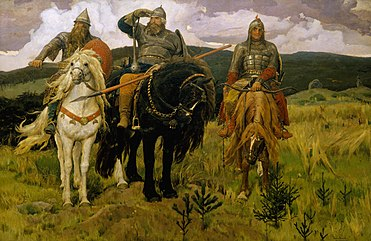
\includegraphics[width=0.49\textwidth]{img/tri_bogatyrya.jpg}
    \end{center}
    \caption{Картина «Три Богатыря» ВМ Васнец\'{о}ва (слева направо: Добрыня Никитич, Илья Муромец и Алёша Попович), ВикипедиЯ.}
\end{wrapfigure}
В центре картины изображён Илья Муромец, народный любимец, герой русских был\'{и}н. Не всем известно, что Илья Муромец не сказочный персонаж, а реальное историческое лицо. История его жизни и \explainDetail{р\'{а}тных}{р\'{а}тный}{military} \explainDetail{п\'{о}двигов}{п\'{о}двиг}{exploit, feat} -- это реальные события. \explain{Впосл\'{е}дствии}{subsequently}, закончив свои труды по охране родины, он стал монахом Киево-Печёрского монастыр\'{я}. Был причислен к л\'{и}ку свят\'{ы}х\footnote{was canonised}. Васнецов эти факты знал, создав\'{а}я образ Ильи Муромца. «\explainDetail{Матёр}{матёрый}{mature, fully grown, hardened} человек Илья Муромец» -- говорит былина. А на картине Васнецова мы видим могучего воина и при том \explainDetail{бесх\'{и}тростного}{бесх\'{и}тростный}{ingenuous, silly} открытого человека. В нём \explainDetail{сочетаются}{сочетаться}{combine} исполинская сила и \explain{великод\'{у}шие}{generosity, magnanimity, goodness}. «А конь под Ильёй \explain{лютый}{fierce} зверь» -- продолжает сказание. \explainDetail{Мощная}{мощный/-ая/-ое}{powerful} фигура коня, изображённого на картине с массивной металлической цепью вместо упряжки, \explainDetail{свид\'{е}тельствует}{свид\'{е}тельствовать}{testify; свидетель: witness} об этом.

Добрыня Никитич по народным преданиям был очень образ\'{о}ванным и \explainDetail{м\'{у}жественным}{м\'{у}жественный}{manly} человеком. С его личностью связано много чудес, наприм\'{е}р, заговорённая броня\footnote{charmed armor} на его плечах, \explain{волш\'{е}бный}{magic} меч-кладенец. Добрыня изображён таким как и в былинах -- величавым, с тонкими, благородными чертами лица, подчёркивающими его культурность, образ\'{о}ванность, \explain{решительно}{decisively} вынимающий меч из \explain{н\'{о}жен}{sheath} с готовностью \explainDetail{бр\'{о}ситься}{брос\'{а}ться/бр\'{о}ситься}{rush} в бой, защищая свою родину.

Алёша Попович \explain{по сравнению с}{as compared with} товарищами молод и строен. Он изображён с \explainDetail{л\'{у}ком}{лук}{bow} и стрелами в руках, но \explain{прикреплённые}{attached} к \explainDetail{седлу}{седло}{saddle} гусли свидетельствуют о том, что он не только бесстрашный воин, но и \explain{гусляр}{player of the musical instrument ``gusli''}, песенник, весельчак. В картине много таких деталей, которые характеризуют образы её персонажей.

Упряжки коней, одежда, амуниция не \explainDetail{вымышленные}{в\'{ы}мышленный/-ая/-ое}{imaginary, fictitious}. Такие образц\'{ы} художник видел в музеях и читал их описания в исторической литературе. Художник \explain{мастерски}{masterfully} передаёт состояние природы, как бы предвещающей о наступлении опасности. Но богатыри представляют собой \explainDetail{надёжную}{надёжный/-ая/-ое}{reliable} и мощную силу защитников родной земли.




\subsection{Картина «Алёнушка» ВМ Васнец\'{о}ва}
% https://muzei-mira.com/kartini_russkih_hudojnikov/1321-opisanie-kartiny-bogatyri-tri-bogatyrya-vasnecova-1898.html

Алёнушка, печальная девочка у \explainDetail{пруда}{пруд}{pond} --- одна из любимых всеми картин В. Васнецова. Художник уд\'{а}чно использует сказочный сюжет, чтобы \explainDetail{раскрыть}{раскрывать/раскрыть}{to open/to discover} сложный и неоднозначный русский характер.

\begin{wrapfigure}{l}{0.4\textwidth}
    \begin{center}
        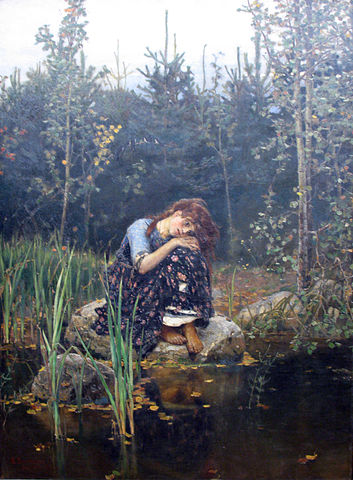
\includegraphics[width=0.38\textwidth]{img/alyonushka.jpg}
    \end{center}
    \caption{Алёнушка, ВикипедиЯ}
\end{wrapfigure}
Грусть девочки очень взрослая. Печаль в её глазах граничит с \explainDetail{отчаянием}{отч\'{а}яние}{despair}. Неубранные рыжие волосы, тёмные глаза, нежно-алые губы --- формируют легко читаемый образ ребёнка с тр\'{у}дной судьб\'{о}й.
В Алёнушке совсем нет ничего \explainDetail{сказочного}{сказочный}{fabulous, fairytale-like}, фантастического.
С\'{о}бственно, вся ск\'{а}зочность сюжета подчеркнута лишь одной деталью --- группой \explainDetail{ласточек}{л\'{а}сточка}{swallow}, сидящих над головой \explainDetail{героини}{героиня}{heroine}. Этим с\'{и}мволом (как известно, л\'{а}сточки символиз\'{и}руют над\'{е}жду) художник \explainDetail{уравновешивает}{уравновешивать/уравновесить}{to balance --- уравнов\'{е}шиваю/-ешь/-ют; уравнов\'{е}шу/-ишь/-ят} полный \explainDetail{тоск\'{и}}{тоск\'{а}}{yearning, longing} \'{о}браз героини, даёт надежду на счастливый финал старой русской сказки.

Васнецов нап\'{о}лнил \explain{ф\'{о}новый}{background} пейзаж атмосферой тишины и гр\'{у}сти.
Отлично удал\'{и}сь художнику в\'{о}дная \explain{гладь}{smooth surface} пруда, \explainDetail{камыш\'{и}}{камыш}{reed}, осока, \explainDetail{ели}{ель}{fir tree}.
Всё \explainDetail{неподв\'{и}жно}{неподв\'{и}жный/-ая/-ое}{still, motionless}, тихо, спокойно.
Даже пруд отраж\'{а}ет героиню очень деликатно, \explain{слегк\'{а}}{slightly}.
Чуть трепещут молодые \explainDetail{ос\'{и}ны}{ос\'{и}на}{aspen}. \explainDetail{Едва}{едв\'{а}}{barely, hardly} \explain{хмурится}{turns gloomly} ос\'{е}ннее небо.
Тёмные, зелёные тона пейзажа контрастируют с \explainDetail{румянцем}{румянец}{blush} на лице героини, а ос\'{е}нняя грусть --- с яркими цветами на юбке Алёнушки. Зритель чувствует: ещё мгнов\'{е}ние и сказка прод\'{о}лжится\dots







\subsection{Картина «Витязь на распутье»}

Виктор Михайлович Васнецов с циклом работ, \explain{посвященных}{dedicated (посвященный + \textit{дат.})} сюжетам русских сказок и былин, оказался \explainDetail{новатором}{новатор}{innovator} в этой области \explainDetail{изобразительного искусства}{изобраз\'{и}тельное искусство}{visual art}. За ним закрепилась репутация «художника-сказочника», он настолько проникся духом русской старины и былинного времени, что свой московский дом построил в виде деревянной избы (сейчас там находится мемориальный музей \explainDetail{живоп\'{и}сца}{живоп\'{и}сец}{painter, artist}).


Картина «В\'{и}тязь на расп\'{у}тье» \explain{отч\'{а}сти}{partly} является и отражением судьбы Васнецова.
Будучи \explainDetail{пр\'{и}знанным}{пр\'{и}знанный}{recognised} художником-передвижником, он, как и его товарищи, \explainDetail{исполнял}{исполнять/исполнить}{performed} жанровые композиции в духе остросоциальных тем, волновавших общество в 1870-1890-х.
Но завладевшая им сказочная тематика диктовала \explainDetail{ин\'{о}е}{ин\'{о}й/ин\'{а}я/ин\'{о}е}{(определительное местоимение) другой, отличный от данного; (неопределённое местоимение) некоторый. See \href{https://ru.wiktionary.org/wiki/\%D0\%B8\%D0\%BD\%D0\%BE\%D0\%B9}{wikictionary.org:иной}.} развитие творчества. Живописец уход\'{и}л от проблем современности и \explain{погружался}{plunge, dive} в мир русской старины, рискуя быть \explainDetail{осужденным}{осужденный}{convicted}.

\begin{wrapfigure}{l}{0.58\textwidth}
    \begin{center}
        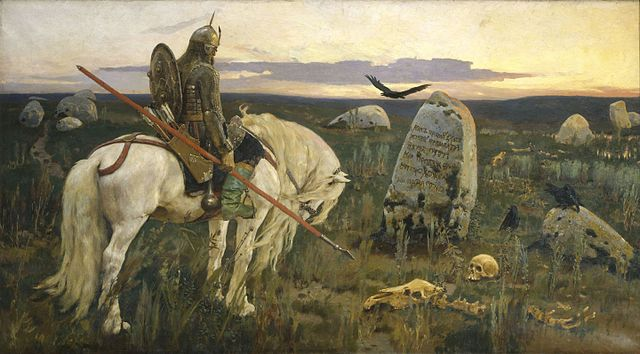
\includegraphics[width=0.57\textwidth]{img/TheKnightAtTheCrossroads.jpg}
    \end{center}
    \caption{Витязь на распутье, ВикипедиЯ}
\end{wrapfigure}
Выбор пути как один из \explain{роков\'{ы}х}{fatal} вопросов человеческой жизни на крупноформатном \explainDetail{холсте}{холст}{canvas} мастера приобрел эпическое звучание.
Перед камнем-предсказателем согнулся под тяжестью фатального \explainDetail{пророчества}{пророчество}{prophecy} опечаленный витязь. \explainDetail{Зловещий}{зловещий}{sinister} в\'{о}рон, садящееся красное солнце нагнетают\footnote{build up the atmosphere} атмосферу. \explainDetail{Нам\'{е}ренный}{нам\'{е}ренный}{intentional} отказ от \explainDetail{изображения}{изображение}{depiction} дороги (как выхода из трудности) художником сделан для того, чтобы показать \explain{неотврат\'{и}мость}{inevitability} судьбы.


\chapter{Путешествия и Туризм}

% --------------------------------------------------
% Туризм
% --------------------------------------------------
\section{Туризм}
Ещё двадцать лет назад немногие люди ездили в отпуск за границу. Большая часть людей проводила отпуск в своей стране. Сегодня ситуация другая, и мир кажется стал намного меньше. Сегодня стало возможным зарезервировать место на морском курорте на другой стороне мира через Интернет.

Не выходя из дома, вы можете \explainDetail{заказать}{заказывать/заказать}{to order (зак\'{а}зываю, -ешь, -ют / закаж\'{у}, зак\'{а}жешь, зак\'{а}жут)} билеты через \explainDetail{сеть}{сеть (ж)}{network} или по телефону. Самолёт \explainDetail{доставит}{доставлять/доставить}{to take sb somewhere} вас прямо туда, куда вы желаете, и через несколько часов после \explain{отбытия} {departure} из своей страны, вы сможете \explain{оказаться}{here: to find yourself} на тропическом \explain{побер\'{е}жье}{coast/bay/shore (побер\'{е}жье, -жья, -жью, -жье, -жьем, -жье)}, \explain{наслаждаясь}{наслаждаться/насладиться: to enjoy (наслаждаюсь, -ешься, -ются)} чистейшим в\'{о}здухом, плавая в кристально чистой, теплой воде тропического моря.

Мы можем путешествовать на автомобиле, поездом или самолётом, если нам \explain{предстоит }{предстоять: to lie ahead} долгая дорога. Некоторые молодые люди предпочитают путешествовать пешком или автостопом, при этом почти ничего не тратя на свое путешествие. Вы встречаете новых друзей, развлекаетесь и \explain{понятия}{понятие: idea} не имеете, где будете завтра. В этом и \explain{заключается}{заключаться/заключиться} большое преимущество для туристов --- тех, кто хочет получить все, что только возможно от исследования мира, \explain{при этом}{while, at the same time} не сильно \explain{утруждая}{утруждать/утрудить: to bother} людей вокруг. Если вы любите горы, вы могли бы подниматься на любые горы по всему \explain{земному шару}{замной шар: earth}. Есть только одно \explain{ограничение}{limitation}. Это деньги. Если вы любите путешествовать, у вас должны быть деньги, потому что это, в действительности, не дешевое хобби.

Экономика некоторых стран существует за счёт туризма. Современный туризм стал высоко развитой индустрией, потому что любой человек любопытен, любознателен и любит \explain{досуг}{leisure}, любит посещать другие места. Именно поэтому туризм процветает.
Люди путешествуют с самого начала своей цивилизации. Тысячи лет назад все люди были \explain{кочевниками}{кочевник: nomad} и собирателями. Всю свою жизнь они \explain{бродили}{бродить/побродить: to wander} \explain{в поисках}{поиск: search} \explain{продовольствия}{продовольствие: food} и лучшей жизни. Таким образом люди \explain{заселили}{заселять/заселить: to inhabit} всю планету Земля.

Так что путешествие и посещение других мест --- это часть нашего сознания. Именно поэтому туризм и путешествие настолько популярны. В настоящее время туризм стал высоко развитым бизнесом. Поезда, автомобили и воздушные реактивные лайнеры, автобусы, суда \explainDetail{предоставляют}{предоставлять/предоставить}{provide} нам комфортное и безопасное путешествие.

Если мы путешествуем \explain{ради}{for the sake of + [gen.]} удовольствия, каждый хотел бы, \explain{во что бы то ни стало}{by all means}, насладиться живописными местами, которые он пролетает, хотел бы увидеть интересные места, насладиться достопримечательностями городов и стран.

В настоящее время люди путешествуют не только ради удовольствия, но также и по делам. Люди должны ехать в другие страны для участия в различных переговорах, для подписания некоторых очень важных документов, для участия в различных выставках, чтобы показать \explain{товары}{товар: merchandise} собственной фирмы или компании. Бизнес-поездки помогают людям получать большее количество информации \explain{относительно}{regarding} \explain{достижений}{достижение: achievement} других компаний, что поможет \explain{создать}{создавать/создать: to create} более успешное дело.

Путешествовать можно по-разному: на корабле, самолёте, автомобиле, пешком. Всё зависит от человека, и его предпочтений.


% --------------------------------------------------
% Салоники
% --------------------------------------------------
\newpage
\section{Что посмотреть в Салониках}
Источник: \url{https://bit.ly/3O5ZooQ}

Для большей части туристов из постсоветского пространства знакомство с Грецией начинается именно отсюда. Международный аэропорт, морск\'{о}й порт, железнодор\'{о}жный вокзал -- Салоники, второй по \ed{величин\'{е}}{величин\'{а}}{size} греческий город, столица области Макед\'{о}ния является крупным транспортным \ed{узл\'{о}м}{\'{у}зел}{node}. Но благодаря богатой истории свои достопримечательности Салоники (Греция) тоже имеет. В городе \explain{сосредот\'{о}чены}{concentrated} памятники трёх эп\'{о}х: эллинист\'{и}ческой, римской и византийской.

Поэтому не стоит, прилетев в Салоники, использовать это место только в качестве транзитного пункта по пути на знамен\'{и}тые греческие курорты, \explain{посвят\'{и}те}{dedicate} и ему самом\'{у} несколько дней. Интересностей в городе Салоники, где древние \ed{раскопки}{раск\'{о}пки}{excavations} можно увидеть во дворе современных жил\'{ы}х кварталов хоть отбавл\'{я}й. \ed{П\'{о}льзуясь}{п\'{о}льзуясь}{taking advantage} советами тех путешественников, кто бывал здесь не однажды, постараемся \explain{провести вас по городу}{to guide you around the city} и \explain{подсказать}{suggest}, что можно посмотреть в Салониках за 3 дня.

\ed{На многих}{на многих}{for many (people)} этот город вначале произв\'{о}дит \explain{противоречивое}{contradictory} впечатление из-за нем\'{ы}сли- мого сочетания эпох и архитектурных стилей. Рядом могут сос\'{е}дствовать красивый парк, цветы, купола старых и новых хр\'{а}мов, древние раск\'{о}пки и тут же -- \explain{ржавые}{rusty} \explain{ограждения}{fences}, неудачные неряшливые граффити на стенах унылых многоэтажек... и вдруг, на стене другого дома -- совершенно оригинальное произведение современного арт искусства! И всё это \explain{чередуется}{alternates} в Салониках, \explain{квартал}{quarter} за кварталом.

Но постеп\'{е}нно нах\'{о}дишь в этой чехард\'{е} и калейдоскопе какую-то особенную гармонию. Некоторые туристы уезжают из Салоников, пон\'{я}в душу этого города и даже немного влюб\'{и}вшись в него.

А наше путешествие только началось. Что посмотреть в Салониках обязательно и никак нельзя пропустить?

\textbf{Прогулка по набережной, Белая Башня и часовой тур по «Культурному маршруту».}
Салоники распол\'{о}жены на берегу \ed{залива}{залив}{gulf} Термаикос. Пройдитесь ранним утром по широкой и красивой набережной, посмотрите на море, порт, рыбаков с \ed{удочками}{удочка}{fishing rod}. Повернувшись лицом к городу, увидите контур самого знакового городского \ed{сооружения}{сооружение}{structures; buildings; constructions}, архитектурного символа и визитной карточки Салоников -- Белую Башню с развивающимся над ней флагом.

И хотя на самом деле она не совсем белая, а «цвета буйволиной к\'{о}жи», история у достопримечательности (XV в) очень занимательная и \explain{заслуживает}{deserves} \ed{отдельного}{отдельный}{individual; separate} рассказа. О ней можно узнать, осмотрев музей, расположенный по кругу на 8 этаж\'{а}х внутри этого 33 метрового (23 м в диаметре) \ed{внушительного}{внушительный}{imposing} сооружения. На самом верху башни смотровая площадка, отсюда открывается красивый вид на набережную, порт и город.

Достопримечательностей в Салониках так много, что только прост\'{о}е \explain{перечисл\'{е}ние}{enumeration} основн\'{ы}х з\'{а}няло бы целую страницу. Но есть замечательная возможность увидеть внушительную их часть даже за 1 час. Конечно, пешком это невозможно, а только сев в автобус №50 тут же, на площади у Белой Башни. Синий экскурсионный автобус отправляется по «Культурному маршруту» каждый час с 8:00 до 21:00. И за 10 евро (5 для детей) в обзорном режиме вы совершите путешествие на машине времени. А остановки (их 8), словно разные эпохи, которые за 25 столетий пережила северная столица Греции. Как нигде, прошлое здесь тесно \explain{соседствует с}{neighbours with} настоящим.

Аудио, видео и гид в автобусе сопровождают экскурсию на английском и греческом. Но для первого визуального знакомства этого достаточно, а в ос\'{о}бо понравившиеся места можно потом вернуться, прихватив с собой карту Салоников с достопримечательностями на русском языке, чтобы не заблудится. Маршрут начинается и заканчивается у башни.

Что же увидят по пути экскурсанты? Недалеко от Белой Башни есть несколько интересных зданий:
\begin{enumerate}
    \item Королевский театр / Национальный Театр Северной Греции
    \item Археологический музей и Музей византийской культуры
    \item Башня телефонной службы
    \item Международная Выставка
    \item Македонский музей современного искусства
\end{enumerate}
Далее по пути чередуются:
\begin{itemize}
    \item памятники эпохи Древнего Рима — раскопки дворца Галерия, Ротонда святого Георгия, \explain{развалины}{ruins} ипподрома и Триумфальная арка, площадь Аристотеля, раскопки римской Агоры
    \item византийские и раннехристианские храмы и памятники – Агия (Святая) София, храм Богоматери Медников (XI в), храм святого Димитрия Солунского; монастыри Салоников – святой Теодоры и Влатадон (XIV в); руины византийских бань.
\end{itemize}

Маршрут проходит мимо площади Аристотеля, Верхнему городу Ано Поли с симпатичными \ed{разноцветными}{разноцветный}{colourful} македонскими домиками.

Об одном из объектов на маршруте по достопримечательностям Салоников расскажем подробнее.

\ed{На заметку}{на заметку}{on a note}! Подборка лучших экскурсий и русскоговорящих гидов в Афинах представлена здесь.

\textbf{Ротонда.} Ротонда святого Георгия постройки конца III века и Триумфальная арка (IV в) – часть дворцового (или погребального) комплекса императора Гая Галерия. В XV веке служила христианской церковью, которая была н\'{а}звана в честь Григория Победоносца. В османские времена турки рядом построили минарет, и почти четыре столетия в храме была \explain{меч\'{е}ть}{mosque}.

В начале XX века здание было возвращено православной церкви, и \explain{с той пор\'{ы}}{since then} здесь Музей христианского искусства. Ротонда находится в \ed{списке}{сп\'{и}сок}{list} памятников Салоников, которые включены ЮНЕСКО в \explain{п\'{е}речень}{list, scroll} объектов Всемирного наследия.

Последнее десятилетие на территории комплекса велись реставрационные работы. Среди описаний достопримечательностей Салоников фото этих работ часто встречаются в рассказах путешественников на форумах. Ведь и во время реставрации в некоторые \explain{помещения}{premises} иногда можно было входить (бесплатно) с камерами, и не запрещалось делать снимки. После официального открытия стоимость входа — 2 евро.

Ротонда находится рядом с Университетским городк\'{о}м, это одно из \explain{мест сбора}{gathering places; venues} и встреч студентов и местной молодёжи.

Утро второго дня и первую его половину можно посвятить каньонингу у Олимпа, а вечером посмотреть спектакль или концерт в Лесном театре.

На заметку! О пляжах \explain{в окрестностях}{in the vicinity of} города Салоники читайте на этой странице, а какой курорт Кассандры (Халкидики) выбрать для пляжного отдыха в этой статье.

\textbf{Лесной Театр.}  Этот театр среди лесных \ed{просторов}{прост\'{о}р}{open space} одно из нескольких \ed{подразделений}{подразделение}{division; unit} NTNG – Национального Театра Северной Греции, в его сост\'{а}ве и театральное училище, прекрасный резерв для \ed{труппы}{труппа}{troupe}. Студенты часто заняты в постановках театра. Посмотреть на спектакль действительно интересно.

Каждый сезон в расписании Театро Дасус премьеры и \ed{прежние}{прежний}{former; old; prior} спектакли собственной труппы, гастрольные выступления других греческих театров.

Кроме собственно театральных постановок здесь весь летний сезон прох\'{о}дят крупные конференции и фестивали, концерты греческих и \ed{заезжих}{заезжий}{visiting} знаменитостей, различные выставки. Такой плотный график и \explain{занятость}{employment; occupation; business} обусловлены отличной акустикой лесной сцены в виде амфитеатра и хорошим техническим оснащением. Количество зрительских мест -- 3894.

Отсюда прекрасные виды на \ed{окрестности}{окр\'{е}стность}{neighbourhood; vicinity} Салоников. И даже если в день вашего посещения нет спектакля или другого мероприятия, всё равно можно прекрасно провести время на свежем воздухе, в кафе, посмотреть окресности, любуясь пейзажами, и привезти домой прекрасные фото достопримечательностей Салоников.

Последний день посвятите шоппингу или просто экскурсии по рынку Модиано, а вечер -- знаменитой Лададике и греческой кухне. И непрем\'{е}нно погуляйте перед отъездом по вечерней набережной.

\textbf{Рынок Модиано.} Modiano Market в Салониках – достопримечательность, часто встречающаяся в \ed{отзывах}{отзыв}{review} и на фото туристов, описания его «\ed{завлекаловок}{завлек\'{а}ловок}{lure/bait}» красочные и вкусные. Если в Салониках у вас есть 3 дня, Модиано – это то место, на которое точно ст\'{о}ит посмотреть.

Хотя рынок и не самый большой, но в остальном по своему колориту и многим признакам напоминает типичный восточный базар. Всё, как там: шум, \explain{гул}{hum; buzz; clatter}, крики торговцев.

Ряды с мясом – полный набор для гурманов-мясоедов. Чуть дальше можно попробовать и купить самый свежий сыр и масло.

Огромнейший выбор оливок: зелёные, чёрные, маринованные, солёные, с приправами и без них, в готовой удобной таре и на развес.

Сезонные фрукты, сладости и \ed{приправы}{приправа}{seasoning} -- каждый найдёт всё, что хотел бы найти.

Но самые интересные -- ряды с \ed{дарами моря}{дар\'{ы} м\'{о}ря}{seafood}. Можно купить свежие морепродукты и тут же, в ближайшей таверне, превратить их во вкуснейший обед. Всё мясо и рыба, продукты, овощи и фрукты на Модиано только местные.

Рынок находится в центре, в начале проспекта Аристотеля (со стороны руин римского форума).

На Модиано много кафе и ресторанчиков, попробуйте вкусно приготовленные греческие блюда и выпейте греческий кофе. Обед обойдётся недорого, даже самый \explain{сытный}{satisfying}. А за трапезой интересно посмотреть на \ed{повседневную жизнь}{повседневная жизнь}{everyday life} жителей Греции и узнавать город и с этой сторон\'{ы}.

\textbf{Лададика.}
Исторический район Лададика -- продолжение набережной и архитектурное наследие Салоников. Злачное место и сосредоточие порочных заведений в прошлом, с начала 2000-х превратилось в один из самых ярких и современных центров ночной жизни в Салониках.

На две части Лададику делит центральная улица Цимиску. Слева остался фрагмент городской стены. Прогуляйтесь по маленьким старинным улочкам. \ed{Изюминка}{из\'{ю}минка}{highlight} этого района Салоников в архитектурном \ed{смешении}{смешение}{mix} стилей середины XIX века и более поздних построек -- именно эта эклектика и привлекает туристов. А с\'{а}ми греки всегда любили проводить здесь время \explain{в праздности}{in idleness; doing nothing}, отдыхая от повседневных \ed{забот}{забота}{worry; concern}.

С 1985 года припортовая Лададика -- охраняемый исторический памятник и строительство новых домов здесь запрещено.

Существующие жил\'{ы}е дом\'{а} отреставрировали предприниматели, открывшие затем свой бизнес на первых этажах отремонтированных стро\'{е}ний. Нижняя часть зданий -- это \explain{ядр\'{о}}{nucleus; core} исторического центра Салоников. Его особый стиль: кованные железные двери \explain{на фоне}{on the background} красного \explain{кирпича}{кирп\'{и}ч}{brick}. Раньше таких домов было много.

Отремонтированы также пол десятка зданий банка Фракия, \ed{склады}{склад}{warehouse} и ангары \explain{переоборудованы}{converted} в магазины и клубы. Открылось немало новых ресторанов, кафе, таверн дискотек и клубов.

Днём местные жители и туристы \explain{ч\'{и}нно}{decorously} попивают здесь кофе, а вечером и ночью открываются двери всех заведений и улочки заливает тёплый жёлтый цвет фонарей. Освещаются открытые террасы в тавернах и кафе. Под бокал вина или стопочку узо, вечер можно провести в уютном ресторане с греческой кухней и живой народной музыкой, здесь их множество. А можно перейти через дорогу и открыть дверь любого клуба, попасть на шумную дискотеку и послушать такой же живой концерт, но в хеви-металл баре.

Почти у каждого \explain{более-менее}{more or less} крупного заведения на Лададике есть свой сайт, и места можно заказать \explain{зар\'{а}нее}{in advance} в сети или по телефону.

Вот и в\'{ы}полнена программа на з дня: «достопримечательности Салоники Греция». И хотя это только малая часть того, что можно посмотреть в этом городе, воспоминания обо всём ув\'{и}денном прочно лягут в \ed{копилку}{коп\'{и}лка}{piggy bank} памяти. И останутся с нами до следующих «каникул в Греции».

Посмотрите видео: \url{https://youtu.be/oObiknNQPUc}



% --------------------------------------------------
% Милос
% --------------------------------------------------
\newpage
\section{Милос – остров Греции с действующим вулканом}

\textit{Источник: \url{https://bit.ly/3OcX6ED}}

Остров Милос обладает уникальными природными красотами и признан греками жемчужиной Эгейского моря. Жители страны и туристы рассказывают об этом курорте с искренним восторгом. Об этом уголке Греции известно многим, ведь именно здесь найдена уникальная статуя богини Венеры Милосской, которая сегодня выставлена в качестве экспоната в Лувре.

\textbf{Общая информация.}
Греческий Милос — один из более 200 островов архипелага Киклады, расположенный в его юго-западной части. Он занимает площадь 16.2 км. кв. Постоянно проживает на острове немного меньше 5000 человек.

Милос имеет вулканическое происхождение и сегодня его характерными географическими особенностями являются причудливой формы скалы с разноцветными горными породами. При этом растительность на острове достаточно скудная, а западная часть острова совсем дикая: здесь не живут люди, из дорог только парочка грунтовых.

\begin{fancyquotes}
    Интересно знать! На Милосе находится один из двух действующих вулканов в Греции.
\end{fancyquotes}

На Милосе очаровательные закаты, естественные пещеры, живописные скалы, чистейшее море с красивыми (хоть и не всегда комфортными) пляжами и, конечно, богатое наследие древнейшей Кикладской архитектуры. Несмотря на перечисленные преимущества, Милос не пользуется большой популярностью у туристов, что привлекает самостоятельных путешественников.


\textbf{Как добраться.}
Остров Милос в Греции расположен на расстоянии 160 км от крупного порта Пирей. Морское сообщение не прекращается даже зимой.

Из Афин добраться на Милос можно на катере или пароме, услуги предоставляют сразу несколько компаний. Дорога занимает около 3,5-6 часов, за это время паром делает несколько остановок, которые позволяют полюбоваться красотами Эгейского моря. В летний сезон количество рейсов паромов увеличивается, поскольку поток туристов растет. Дополнительно предусмотрены рейсы на острова Кикладского архипелага. Расписание нужно узнать заранее, билеты можно забронировать в режиме онлайн одном из сайтов перевозчиков: \url{www.seajets.gr}, \url{www.minoan.gr}, \url{www.zanteferries.gr}, \url{www.bluestarferries.com}, \url{https://aegeanspeedlines.gr}, \url{https://goldenstarferries.gr}.

На Милосе есть аэропорт, который круглый год принимает рейсы из Афин, а в теплое время года сюда прилетают чартерные рейсы.

\textbf{Достопримечательности острова.}
На острове много пляжей, но это не единственная причина, по которой следует посетить Милос в Греции.

В порт Адамантас прибывают все паромы из других точек страны. В городе туристам предлагают экскурсионные туры в разные точки острова, а также морские круизы вокруг Милоса.

\textbf{\ed{Бухта}{б\'{у}хта}{bay} Клефтико.}
Пожалуй, самые яркие впечатления вызывает экскурсия на яхте к бухте Клефтико, расположенной на юго-западе острова. Бухта примечательна белоснежными скалами и пещерой, которая служила прибежищем для пиратов.

Добраться до бухты можно и самостоятельно по суше, но для этого придется пройти небольшой квест – арендовать внедорожник или квадроцикл, проехать часть пути по бездорожью, а затем идти пешком еще 40-60 минут. Больше подробностей узнайте из видео внизу страницы.

\textbf{Город Плака.}
Столица острова – город Плака — находится на высоте более двухсот метров над уровнем моря. С его высоты открывается панорамный вид на залив. Яркой достопримечательностью города считается замок крестоносцев, который находится неподалеку от церкви Богородицы Таласситры.

В южном направлении от Плаки расположены руины древнего поселения Мелоса. Здесь сохранились остатки римского театра и храма. В 1820 году в развалинах города была найдена та самая статуя Венеры, которою сегодня можно увидеть в парижкском Лувре.

\textbf{Природные пещеры.}
Пещеры острова заслуживают отдельного повествования. Сикия – самая необычная пещера, расположенная в западной части Милоса. Сюда регулярно следуют яхты и корабли из Адамантаса, также есть дорога со стороны церкви Святого Иоанна.

Самым посещаемым местом является пещера, образованная четырьмя скалами. Из Адамантаса сюда привозят экскурсии.

В южном направлении от Милоса расположен островок Антимилос, тут разводят ослов редкой породы.

\textbf{Церкви острова Милос.}
Агиоса Николаоса в Адаманте – при церкви работает музей. Святого Харлампия в Адаманте – здесь хранятся древнейшие иконы византийской эпохи. Панагия Корифиатисса в Плаке – построена в 1810 году, отсюда открывается волшебный вид на залив. Панагия тон Родон или Розария – храм украшен во французском стиле. Самый живописный храм на острове – Панагия Фаласситра. Часто на фото острова Милос в Греции часто можно увидеть именно эту церковь. Святого Харлампия в Плакесе славится древними, красивейшими фресками и росписями. Агиос Спиридонас в поселке Триовассалос – на Пасху здесь проводят театральное представление, во время которого сжигают куклу Иуды.
Профити Илиас (Пророка Ильи) в поселке Клима примечательна мраморным фундаментом.
Панагия Портиани в поселке Зефирия – в прошлом храм был митрополитским собором, сегодня находится под охраной Министерства культуры Греции.

\textbf{Музеи острова Милос.}
\begin{enumerate}
    \item Археологический музей. Находится на центральной площади столицы острова. В качестве экспонатов представлены скульптуры, древнее оружие, керамика, украшения. Вход 2 евро.
    \item Церковный музей. Коллекция экспонатов представлена древними византийскими иконами, богатым церковным одеянием и уникальными реликвиями. Вход свободный.
    \item Фольклорный музей. Находится на центральной площади столицы в здании XIX века. Экспонаты – предметы обихода и изделия народного творчества, демонстрирующие культуру и обычаи греческого народа. Вход 4 евро.
\end{enumerate}

\textbf{Поселки на острове.}
Живописное рыбацкое поселение на Милосе в Греции, расположено в тихой бухте, защищенной скалами. Людей здесь очень мало. А немногочисленные отели выглядят, как настоящие рыбацкие домики. Пляж Фиропотамоса чистый, без волн, в цвет воды особенно радует глаз.

\textbf{Клима.} Клима – самая большая рыбацкая деревня. Колоритное место, где дома построены у самой кромки воды, первые этажи построек используются в качестве гаражей для лодок. Двери и балконы домов выкрашены в разные цвета, благодаря чему весь поселок выглядит ярко и привлекательно. Сюда стоит приехать, чтобы сделать колоритные фото.

Деревня Плака, словно, приклеилась к склону горы, ее внешний вид больше всего напоминает традиционную Грецию – белые дома с синими дверями и ставни, украшенные цветами. На вершине городка находится венецианский храм и открывается живописный вид на Милосский залив. Столицу острова Милос лучше всего осматривать, просто прогуливаясь по узким улицам.

\textbf{Трипити.}
Ранее здесь проживали ремесленники, сегодня в поселении туристы посещают древнее христианское кладбище – лабиринт из многочисленных ходов в пещере.

В поселке есть и удобный песчаный пляж, и широким выбором ресторанов, кафе и отелей. Также в Трипити есть, что посмотреть: милосские катакомбы, руины античного театра, церковь Святого Николая и ветряные мельницы на окраинах. При желании все достопримечательности можно обойти пешком.

\textbf{Пляжи.}
Милос славится комфортабельными пляжами, их по всей территории острова более 70. Большинство пляжей появились в результате вулканической активности. Если дует ветер с севера, идеальные для отдыха пляжи – Фириплака, Циградо, Палеохори, Айя Кириаки. При южном ветре лучше отдыхать на пляжах – Саракинико, Митакас и Фиропотамос.

Фиропотамос. Находится в одноименной деревушке, где часто собираются яхтсмены и рыбаки. Пляж удобный для отдыха, здесь развитая инфраструктура и есть деревья, создающие тень.

Саракино. Один из самых живописных пляжей. Находится в бухте, которая ранее использовалась пиратами. Над пляжем нависают белоснежные скалы. Укрыться в тени здесь практически невозможно, это место любят романтические пары.

Палеохори. Один из самых и посещаемых пляжей. Мягкий, мелкий песок окружен разноцветными скалами. Для отдыхающих предусмотрены шезлонги и зонтики, работает Центр виндсерфинга.

Фириплака. На этом пляже любят отдыхать семьи с детьми. Расположен в южной части острова, здесь почти никогда не бывает волн и порывов ветра. Берег образован разноцветными скальными породами.

Айя Кирияки. Живописный пляж с широкой береговой линией и чистейшей водой, окружен скалами. Неподалеку много кафе и ресторанов. Этот пляж создает впечатление уединенного места.

Папафрагас. Пляж находится в крошечной бухте, прибрежная полоса тоже небольшая, уютная. Добраться сюда достаточно сложно, поскольку спуск крутой и узкий. Но, проделав такой путь, вы будете вознаграждены удивительным видом.

\textbf{Климат и погода.}
На острове традиционный для Средиземноморья климат. Летом здесь жарко и сухо, а зимой – мягкая и дождливая погода.

Летом на острове дует освежающий северный ветер Мельтеми. Это сезонное явление, которое начинается во второй половине июля и длится до конца августа. Таким образом, в самый жаркий сезон на Милосе нет изнуряющего зноя.

Оптимальное время заняться изучением вопроса – как добраться до Милоса в Греции – между Пасхой и началом сентября. В мае средняя температура составляет +21 … +23 градус, вода в море прогревается до +18 … +19 градусов. В наиболее жаркие месяцы – июль-август – воздух прогревается до +30 градусов, а вода – до +26 град.

Если вам приходилось смотреть фильм «Пеликан», вы наверняка запомнили сказочные греческие пейзажи. Именно Остров Милос стал местом, где проходили съемки картины. Еще один повод посетить курорт – его форма. Милос похож на подкову, возможно, поездка сюда принесет вам счастье и удачу.

Больше интересной и полезной информации об о. Милос и его пляжах узнайте, посмотрев видео!

Видео: \url{https://youtu.be/U0D-1ijdS3E}




\newpage
\section{Герб Междуреченска}
В 1966 году был объявлен конкурс на лучший герб города, в котором было рассмотрено 59 эскизов. После рассмотрения представленных эскизов лучшим был признан проект герба под № 48, который городской комитет ВЛКСМ и предложил для утверждения.


\includegraphics[width=0.3\textwidth]{img/Flag_of_Mezhdurechensk_(Kemerovo_oblast).png}

Автор герба Вадим Гущин, несмотря на нарушение ряда важных законов геральдики, сумел просто и оригинально, отказавшись от традиционных для того времени шестерёнок, колб, отбойных молотков, отразить промышленную специфику, совместив её с природно-географическим положением города.

28 августа 1966 года газета «Знамя шахтёра» представила жителям Междуреченска герб: «Щит разделён на два поля: красное (вверху) — цвет труда и зелёное (нижнее) — цвет тайги. В свете вспыхнувшей искры кусок угля — главного нашего богатства. На зелёном поле — две голубых ленты — Томь и Уса. Таким образом, герб олицетворяет две главнейшие особенности города — направленность труда его жителей и природные условия».

Автор герба совершил небольшую ошибку. Дело в том, что река Уса впадает в реку Томь с её правого берега. В гербе 1966 года сходящиеся реки изображены текущими в левую геральдическую сторону (от зрителя — в правую), что не соответствовало действительности. Ошибка была исправлена, и 18 марта 1993 года был утверждён изменённый герб.


\section{Кошмар началс\'{я} на второй день}

\textit{Мария Гейн}

\textit{Истории туристов, которые решили бесплатно пожить у местных}

\textit{Истончик: \url{https://lenta.ru/articles/2022/09/27/couchsurfing/}}

За последние 20 лет сервис для поиска бесплатного \ed{ночл\'{е}га}{ночл\'{е}г}{overnight stay} в поездках CouchSurfing \explain{снискал популярность}{gained popularity} у путешественников по всему миру. Для многих такой формат поездок стал не только способом сэкономить \ed{приличные}{приличный}{decent} деньги на отелях, но и возможностью лучше узнать новый город или страну. Тем не менее каучсерфинг может оказаться настоящим испытанием для \ed{неподготовленного}{неподготовленный}{unprepared} туриста — форумы \ed{пестрят}{пестрить + чем?}{are full of} историями о неадекватных хозяевах и ужасных условиях, в которых оказались путешественники. Как решиться на каучсерфинг, насколько опасен такой формат путешествий и чем может обернуться ночлег у незнакомца — в материале «Ленты.ру».

\textbf{От хиппи до диванных \ed{скитальцев}{скиталец}{wanderer}}

Идея \ed{бескорыстного}{бескорыстный}{selfless, disinterested; here бескорыстное гостеприимство: selfless hospitality} гостеприимства родилась \explain{задолго до}{long before} появления интернета и \explain{восходит к}{dates beack to} эпохе хиппи. Не обремененные деньгами и стабильностью, они не имели средств на гостиницы и путешествовали в основном \explain{автостопом}{hitchhiking}. Чтобы не остаться без крыши над головой, хиппи вели так называемые рингушники — записные книжки с адресами и телефонами людей в разных городах, у которых можно было бесплатно погостить некоторое время.

Рингушники были \explain{едва ли}{hardly} не самой важной и постоянной частью жизни хиппи — их тщательно пополняли новыми адресами, а имена \ed{надёжных}{надёжный}{reliable} людей передавали из рук в руки. Позже привычку вести такие записные книжки переняли автостопщики, студенты и все, кто хотел объехать мир за копейки. Все изменилось с появлением интернета.

В основе создания сервиса CouchSurfing лежит красивая история об американце Кейси Фентоне, который отправился в путешествие мечты. В 1999 году 21-летний молодой человек, выросший в семье хиппи, купил дешёвые авиабилеты из Бостона в Исландию. \ed{Осознав}{осознав (осознать)}{realising}, что денег на гостиницы не хватает, молодой человек проявил \explain{изобретательность}{ingenuity, inventiveness}. Он раздобыл базу email-адресов Исландского университета и \explain{разослал}{sent out} сотню писем с просьбой приютить его бесплатно.

К удивлению Фентона, на его письмо \explain{откликнулись}{Откл\'{и}кнуться (откл\'{и}кнусь, откл\'{и}кнешься, откл\'{и}кнутся) / Отклик\'{а}ться (отклик\'{а}юсь, отклик\'{а}ешься, отклик\'{а}ются): to respond (e.g., to email)} десятки студентов. Добрые исландцы даже составили ему готовый план поездки, согласно которому он должен был перемещаться по стране от дома к дому. \explain{Воодушевлённый}{encouraged (by)} исландским \ed{радушием}{радушие}{cordiality}, Фентон решил подарить другим путешественникам такой же опыт.

После возвращения домой он зарегистрировал домен и придумал название проекта. Слово CouchSurfing буквально означает «путешествие по чужим койкам» и состоит двух частей: couch, что в переводе с английского означает диван и surfing — кататься на волне или \explain{странствовать}{wander}. Именно поэтому в народе каучсерферов стали называть диванными скитальцами.

\begin{fancyquotes}
    Словарь каучсерфера\\

    \textit{Хост} — хозяин, принимающий у себя путешественников\\

    \textit{Реквест} — запрос о ночлеге, который путешественник отправляет потенциальному хосту\\

    \textit{Вписка} — непосредственно сам ночлег\\

    \textit{Серфер} — человек, который ищет бесплатное жилье в поездке
\end{fancyquotes}

Пробную версию сайта запустили в 2004 году, в разработке Фентону помогали друзья и единомышленники. За первый год на платформе зарегистрировались 6000 пользователей, на следующий — уже 20 тысяч. CouchSurfing быстро завоевал популярность у бэкпэкеров сначала в Европе и США, а потом стал активно использоваться в Азии, Африке и Латинской Америке.

Спустя почти 20 лет после запуска популярность сервиса продолжает расти. Если верить данным «Википедии», на нем зарегистрировано 12 миллионов пользователей более чем из 200 тысяч населенных пунктов по всему миру — даже на далеком острове Пасхи путешественников готовы принять почти 60 хостов.

Слово «каучсерфинг» плотно вошло в обиход и стало нарицательным — сейчас так называют формат цифрового гостеприимства, когда жители какой-либо страны или города предоставляют безвозмездный ночлег путешественникам.

Помимо непосредственно самого сайта CouchSurfing.com существует несколько аналогичных сервисов. На некоторых при регистрации нужно платить символический членский взнос, где-то — проходить собеседование. Самыми известными альтернативами считаются BeWelcome, Servas International и Trustroots. Есть и более нишевые проекты: например, Warm Showers создан для велопутешественников, а Pasporta Servo — для любителей искусственно созданного языка эсперанто.

Найти хоста также можно на форумах или в социальных сетях — во «ВКонтакте» и на Facebook (запрещена в России; принадлежит компании Meta, которая признана экстремистской организацией и также запрещена в стране) есть множество тематических групп для поиска ночлега в отдельных странах и городах. Однако опытные путешественники предупреждают, что такой способ «вписаться» не всегда безопасен. Если CoushSurfing и подобные сервисы стремятся обеспечить максимальную прозрачность путем верификации учетной записи и системы оценивания хостов, то в соцсетях можно с легкостью нарваться на людей с не самыми чистыми намерениями.

Тем не менее, несмотря на все предосторожности и протоколы безопасности CouchSurfing, ночлег у незнакомых людей может иметь неприятные последствия. Одна из нашумевших историй произошла в 2009 году. Туристка из Гонконга приехала в Великобританию и договорилась о «вписке» в Лидсе — хостом оказался мужчина марокканского происхождения. Он два раза изнасиловал девушку и едва не убил ее. Мужчину приговорили к десяти годам тюрьмы.

Другой случай с CouchSurfing, поставивший под сомнение репутацию сервиса, произошел в Италии в 2014 году. Представившись выдуманным именем, местный житель пригласил в гости 16-летнюю девушку-подростка из Австралии, накачал ее наркотиками и изнасиловал. В ходе судебного разбирательства выяснилось, что мужчина не раз пользовался доверчивостью туристок и заманивал их к себе домой с помощью анкеты на CouchSurfing.

\textbf{Правила хорошего тона}

Страх столкнуться с неадекватным хостом или вовсе нарваться на маньяка часто отпугивает туристов от каучсерфинга. Чтобы максимально себя обезопасить, необходимо придерживаться нескольких принципов. Самое базовое — это внимательно изучить профиль хоста, прочитать отзывы и поделиться его контактами со своими близкими.

\begin{center}
    \Large
    Когда в профиле мужчины напрямую говорится о желании принимать только девушек, а в графе интересов стоит секс — есть повод насторожиться. Также стоит заранее пообщаться с хостом: выяснить, где придется спать (в отдельной комнате или вместе с хозяином), и попросить прислать фото
\end{center}

Как рассказала «Ленте.ру» клинический психолог, эксперт в сфере домашнего насилия, посттравматического стрессового расстройства и зависимостей Олеся Иневская, важно избегать ситуации зависимости от хоста. «У вас должны быть деньги на запасной вариант ночлега не только на случай конфликта или странного поведения хоста, но и на случай отказа. У хоста могут случиться непредвиденные ситуации непосредственно перед заселением», — посоветовала эксперт.

Кроме того, в среде каучсерферов есть негласные правила хорошего тона, соблюдение которых сделает пребывание в чужом доме комфортным. В каучсерфинге все находятся на равных, поэтому важно не злоупотреблять гостеприимством и не нарушать личные границы. Брать продукты без спроса, надолго занимать ванну и приходить в дом в грязной одежде — не лучший способ найти общий язык с хостом.

\begin{fancyquotes}
    Необходимо узнать культурные особенности и обсудить детали проживания: распорядок дня, бытовые условия (как хозяин дома потребляет воду и электричество), количество ночей и время вашего отъезда. Предвидеть, что может стать нарушением границ, практически невозможно

    \begin{flushright}
        Олеся Иневская, клинический психолог
    \end{flushright}
\end{fancyquotes}

Беспроигрышный вариант поладить с хозяином дома — привезти сувениры из родной страны или города, особенно ценятся съедобные подарки. «Предложите хосту совместно приготовить ужин национальной русской кухни, расскажите о традициях. Это станет хорошим выражением благодарности за то, что человек принимает вас у себя дома», — рекомендует практический психолог и член ассоциации когнитивно-поведенческих психотерапевтов Татьяна Сушкова.

Несколько россиян поделились с «Лентой.ру» своим опытом каучсерфинга и рассказали о самых курьезных и жутких случаях.

\textbf{«Буду мыть за вас посуду и травить байки о Путине»}

\textit{Василий, объехал по каучсерфингу две страны}

Началось все с путешествия по Испании. Я был классическим бедным студентом, который решил попутешествовать по Европе. Выбор пал на Испанию, которая была бюджетнее других стран ЕС. За три недели я побывал в Овьедо, Бильбао и Барселоне. Скачав приложение CauchSurfing, я столкнулся с проблемой. Так как я был новым пользователем с нулевым рейтингом, на мои запросы никто не отвечал. Чтобы привлечь внимание хостов, я обещал привезти из России угощения и рекламировал себя в качестве уборщика. К моему удивлению, в Барселоне меня приютили после шуточного предложения рассказывать анекдоты о российском президенте.

Второй страной, где я ни разу не бронировал гостиницу, стала Бельгия. Это маленькое государство, поэтому я решил найти «вписку» где-нибудь в центре и каждый день ездить в новый город. Мой выбор пал на Гент — небольшой средневековый городок с каналами и удобным расположением с точки зрения железных дорог.

Моим хостом стал пожилой фермер-фламандец Ксандр, который почти не говорил по-английски. Он поселил меня в крытый загон для лошадей, который уже не использовался и был оборудован для приема гостей. Хотя к сырости и не совсем приятному запаху пришлось привыкать, там было все необходимое для жизни: кровать, полки для вещей, туалет и даже что-то, напоминающее душ. По утрам Ксандр устраивал завтраки с фермерскими продуктами и в целом оказался очень милым стариком.

Для меня каучсерфинг — это история в первую очередь про авантюризм, ведь ты никогда не знаешь, что будешь делать. Хост может провезти тебя по тем местам, куда не добираются обычные туристы. В том же Генте хост со своим другом устроили мне бесплатную экскурсию по каналам на яхте.

\textbf{«Он напился и лег ко мне в кровать»}

\textit{Инна, убежала от хоста посреди ночи}

Я пользовалась сервисом CauchSurfing.com один раз, когда в 22 года поехала в одиночное путешествие во Францию. Скажу сразу — в этой поездке сбылись мои самые худшие опасения, все не задалось с самого начала. Я договорилась с мужчиной средних лет из Конфлан-Сент-Онорина (пригород в 30 километрах от Парижа) о «вписке» на два дня.

Мы условились встретиться возле его дома в определенное время, но он опоздал на полтора часа. Француз Анри жил в уютной чистенькой студии. Единственное, что меня смущало. — это перспектива спать с ним в одной комнате, пусть и не в одной кровати. Он любезно уступил мне большой раскладной диван, а сам устроился на раскладушке.

\begin{center}
    \Large
    Кошмар начался на второй день, когда он вернулся далеко за полночь с какой-то вечеринки, едва стоя на ногах. Я проснулась от резкого запаха перегара — Анри лежал почти вплотную ко мне и спал. Решение разбудить его оказалось ошибкой
\end{center}

Он не домогался меня и не пытался изнасиловать, но вел себя крайне неадекватно: кричал что-то на французском, ходил по квартире, открывал и закрывал окна. Мне стало банально страшно оставаться с пьяным человеком на 30 квадратных метрах, поэтому я собрала рюкзак и ушла. Было почти пять утра, пришлось ждать открытия кафе, чтобы позавтракать и спокойно умыться. Днем у меня был поезд в Нант, где меня ждала койка в хостеле. С тех пор каучсерфингом я не пользовалась.

\textbf{Не ради денег}

Если с туристами, которые хотят сэкономить на отелях и глубже погрузиться в другую культуру, все понятно, то что движет людьми, готовыми впустить в дом совершенно незнакомых людей?

По словам Вадима из Санкт-Петербурга, который за четыре года принял у себя 13 человек, каучсерфинг — это окно в мир. «До пандемии у меня останавливалось много иностранцев. Тогда я не мог позволить себе отдыхать за границей, поэтому это была возможность близко познакомиться с чужими культурами. Еще один плюс — ты начинаешь по-другому смотреть на свой город. У меня жила пара французов, которая попросила свозить их в Кронштадт. Сам я был там последний раз на экскурсии в седьмом классе и был приятно удивлен, как там все изменилось», — поделился он в беседе с «Лентой.ру».

\begin{fancyquotes}
    Приятный бонус — подарки от путешественников. Как-то два испанца привезли мне три килограмма хамона в знак благодарности
\end{fancyquotes}

Другие опытные хосты рассказывают, что принимают у себя людей ради практики иностранных языков. Например, Виктория из Новосибирска, закончившая институт востоковедения, успела «вписать» к себе 18 туристов из Китая.

«Конечно, неприятные случаи тоже бывали. Однажды, когда меня не было дома, парень из Харбина решил приготовить на моей кухне вок. Видимо, что-то пошло не так, и он испортил дорогую сковородку с антипригарным покрытием», — рассказывает девушка. Чтобы избежать подобных случаев, Виктория рекомендует сразу очертить путешественнику границы дозволенного. Например, брать книги, пользоваться кофемашиной и утюгом — можно, брать средства личной гигиены и продукты из холодильника — нет.

«Сразу видно людей, которые подались в каучсерфинг только ради халявы и воспринимают твой дом как бесплатный отель. Уже на этапе реквеста они много спрашивают про условия проживания и по минимуму говорят о себе. Скорее всего, такой человек даже не помоет за собой посуду, ведь будет считать тебя "персоналом"», — добавила Виктория.

Она подчеркивает, что к поиску «вписки» стоит подходить вдумчиво: не рассылать одинаковые заявки хостам, а делать их индивидуальными — благодаря этому каучсерфинг станет незабываемым опытом для обеих сторон, а не просто бесплатным ночлегом.

\begin{center}
    \Large
    Если хотите оставить после себя грязную посуду и скомканные простыни, идите на Airbnb
\end{center}

Как бы то ни было, каучсерфинг — гораздо больше, чем способ экономить в поездках, это целая философия путешествий и гостеприимства. Сейчас этот сервис может быть особенно полезен российским туристам, поскольку платить за отели за границей без карты иностранного банка невозможно, да и забронировать экскурсии по городу дистанционно не получится. В таких ситуациях хост может не только выручить с жильем, но и показать локальные достопримечательности и заведения.

\newpage
% Достопримечательности Москвы: что посмотреть и где гулять
\section{Достопримечательности Москвы}

\textit{Лана Ржевская\\
    Познаёт Москву каждый день}

\textit{Источник: \url{https://travel.yandex.ru/journal/moscow/}}

В столицу приезжают, чтобы ощутить историю и гордость за страну, побывать в значимых местах и увидеть, как меняется город, почувствовать его креатив и стремление к новому. Даже если вы приезжали в Москву или живёте в столице, всегда можно найти новые интересные точки, события, окружение, возможности.

В подборке 30 знаковых, модных и романтичных мест Москвы для молодёжи и семей с детьми, для традиционных и креативных путешественников. Здесь гуляют и развлекаются, получают новые эмоции, ощущения и знания.


\textbf{Достопримечательности Москвы: что посмотреть и где погулять.} Москва --- это город, в котором \ex{уживаются}{coexist, get along} средневековые \ex{улочки}{streets} XVI века и небоскрёб с самой высокой смотровой площадкой Европы, где в бывшем хрустальном заводе или шоколадной фабрике создают креативные пространства, а светский клуб --- это не лимузин и фрак, а кино в ночи и танцы под винил.

Здесь 500 лет хранит историю Грановитая палата, названная по белому камню на фасаде, теснённому на 4 грани. В Новый год на улицах \ex{наряжают}{(here) decorate} более 500 ёлок. Направляясь в Москву из Нижнего Новгорода, вы проедете то же расстояние, что и путешествуя по всем линиям московского метро, 450 км. А чтобы пройти пешком все улицы Москвы, понадобится не один месяц, ведь это более 6000 км.

В Москве почти 450 музеев и около 10 000 ресторанов, кафе и баров. В десятках парков можно угоститься вкусным кофе и фирменными пончиками. Или посетить международные выставки, соревнования и марафоны. И это очень нравится 12 миллионам москвичей и 20 миллионам туристов, которые ежегодно посещают самый большой российский город.

Знакомство с Москвой традиционно начинают с центра города --- Кремль и всё, что его окружает, неизменно привлекают туристов. Вряд ли найдётся в мире другая столица с главной крепостью на 27 гектарах и окружающим её центром, одновременно историческим и абсолютно современным.

\textbf{Красная площадь.} На этой площади узнавали царские указы и городские новости, провожали и встречали воинов, по указу Петра I показывали образец украшения новогодней ёлки и «огненных праздничных утех», проводили \ed{крестные ходы}{Крестный ход}{в православных и восточнокатолических церквях торжественное церковное шествие с большим крестом (от его несения в начале процессии она и получила своё название), иконами и хоругвями вокруг храма или из одного храма в другой (например, в Пасхальную неделю вокруг церкви, в Крещение на водосвятие), или от одного места к другому (например, от храма к реке для освящения воды, от захоронения мученика к освящению нового храма его имени, вокруг городов и т. д.).} и казни.

Площадь появилась благодаря крупному пожару, уничтожившему постройки с этой стороны кремлёвской стены. Долго в народе так и говорили --- на Пожаре, имея в виду на площади, где был тот самый пожар. Здесь торговали и нанимали попов для службы на дому.

Название «Красная» она получила как статус главной площади Москвы, но такой красивой, как сейчас, стала значительно позже.


Сейчас Красная площадь, знакомая по парадам и новогодним курантам, влечёт всех приезжающих в Москву. Она открыта для посещения в те дни, когда нет мероприятий. Но сюда можно попасть и во время концертов или праздников — можно купить билеты, например на этом сайте\footnote{\url{https://mos-kassir.ru/place/krasnaia-ploshchad.html}}.

Традиционные мероприятия --- августовский фестиваль военных оркестров «Спасская башня», сентябрьский концерт ко Дню города, ноябрьский фестиваль Средневековья и рыцарский турнир, декабрьская ГУМ-ярмарка и празднование Нового года с салютом, фестиваль «Московская Масленица» и празднование Пасхи, репетиции Парада и сам Парад, концерт в День России, июльский цветочный фестиваль.

\textbf{Кремль.} Когда-то на месте Кремля была Ведьмина гора с языческим ритуальным столбом. Обряды на горе пророчили младенцам — здоровье, воинам — силу. При Иване III началось масштабное строительство крепости на холме. Сейчас Кремль --- это 20 башен, 28 гектаров земли и 2235 метров кремлёвской стены высотой до 19 метров и толщиной до 6,5 метров.

Вход в Кремль --- через Кутафью башню. Внутри крепости можно увидеть мощёные площади и уютные скверы, дворцы и храмы, которым не одно столетие. А ещё --- знаменитый Царь-колокол, который не звонил, и Царь-пушку, которая не стреляла.

На Соборной площади в 12 часов по субботам, с мая по сентябрь, можно увидеть почётный караул. Церемония развода пешего и конного караула --- яркое и запоминающееся зрелище: военный оркестр, исторические мундиры времён Николая II, холёные гордые кони, эффектная конная карусель, всё торжественно и патриотично. В середине церемонии будет громко, готовьтесь.

Сидячих мест нет. Чтобы лучше видеть церемонию, заранее займите место поближе к ограждению. Купить комплексный билет на осмотр Соборной площади и билеты в музеи Московского Кремля можно на сайте. Цена от 700 рублей.


\textbf{Манежная площадь, Манеж: Часы мира, шопинг и выставки.} Манежная площадь всегда была шумной и торговой. Названия близлежащих улиц тому подтверждение: Моховая, где торговали мхом, Обжорный ряд, Лоскутный переулок. Сейчас вся торговля перенесена под Манежную площадь в 3-этажный торговый комплекс «Охотный ряд».

Хорошо, что «Манежка», как называют \ex{ТЦ}{торговый центр}, не стала только бутиковой, как ЦУМ с его шикарными витринами и космическими ценами. Здесь много популярных сетевых магазинов с доступными ценами, акциями и скидками. Потому и не пустует, торговля идёт оживлённо.

Интересны стеклянные купола над торговыми рядами. Они изготовлены из высокопрочного технического стекла, сквозь них в ТЦ проникает естественный свет.

На полусфере фонтана «Часы мира» изображена карта. Чтобы узнать, какое сейчас время в выбранном городе, нужно провести воображаемую линию вниз до неподвижного кольца вокруг купола. На нём числа от 1 до 12 — это час. Количество светящихся оконцев над часом, умноженное на 5, это минуты. В итоге получаются часы и минуты в выбранном городе.

Здание Манежа изначально предназначалось для строевых тренировок солдат и офицеров. И сразу стало архитектурным чудом: 45-метровое здание накрыто одним куполом на деревянном каркасе, без каких-либо дополнительных опор. Потом Манеж сменил амплуа: стал местом народных гуляний и концертов, хотя недолго был даже гаражом для машин правительственных кортежей.

Посмотреть расписание мероприятий и купить билеты можно на сайте. График работы вт-вск с 12:00 до 22:00.

\textbf{Площадь Революции.} Её ориентиры — 2 музея и 2 отеля. Музей Отечественной войны 1812 года и Исторический музей с одной стороны, гостиницы «Москва» и «Метрополь» с другой. Пять столетий назад посередине площади протекала река Неглинная, по берегам шла оживлённая торговля в рядах — яблочном и дынном, капустном и ягодном. Позже реку убрали в подземный коллектор, а Воскресенский мост разобрали. А вот Воскресенские ворота остались: около них находится символичный «Нулевой километр», где приезжие кидают монетку, чтобы вернуться.

Бывшая Воскресенская площадь была переименована в марте 1917 года, когда после отречения Николая II в здании Городской Думы создали революционный комитет. На площади стали собираться тысячи демонстрантов.


Несмотря на революционное название, сейчас у площади нет политического подтекста. Напротив, она стала местом проведения городских фестивалей и праздников. Например, летнего фестиваля цветов, осеннего праздника урожая с креативными арт-объектами из даров осени, рыбной или сырной недели. Детская ярмарочная карусель и аниматоры радуют детей, взрослые делают покупки и дегустируют деликатесы.

\textbf{Александровский сад.} После многолюдной Манежной площади приятно отдохнуть в спокойной зелени Александровского сада.

Войдите в Верхний сад через главные ворота с золочёными двуглавыми орлами на столбах.


В Саду несколько точек, связанных с военной историей. Памятные плиты городов-героев, итальянский грот «Руины», который символизирует военную победу и возрождение Москвы после войны 1812 года.

Самая популярная фотолокация Александровского сада — фонтанный ансамбль с каскадами, сказочными героями и «Гейзером».

В Среднем саду, от Кутафьей башни до Боровицкой, расположены кассы музеев Кремля, уютные лавочки для отдыха, сувенирные магазины.


\clearpage

\section{Иммиграция}

\textit{Россияне рассказывают, каково это — жить вдали от родины}

{
    \it В рубрике «Из жизни» каждую неделю публикуются рассказы людей, которые по разным причинам решили переехать в другие страны. Одни отправились за границу в поисках любви, другие уехали на время обучения, а третьи просто решили, что вдали от родины их ждет лучшая жизнь.
}

\textit{Источник: \url{https://lenta.ru/themes/2018/02/12/migration/}}

\subsection{Япония}
% --- Studied 
% --- Added to Anki

\textit{«Русские мерзнуть не могут — кожа особенная» История россиянки, перебравшейся в Японию}

Рина переехала в Японию сразу после университета и влюбилась в страну с первого взгляда. Вопреки стереотипам о не подпускающих к себе японцах она стала своей в небольшом городке, а позже — успешно ассимилировалась в мегаполисе. В рамках цикла материалов о россиянах, перебравшихся за границу, «Лента.ру» публикует ее рассказ о жизни в Токио.

После окончания университета — в тот момент я находилась в Бельгии — мне захотелось продолжить свой жизненный путь за границей. Мне казалось, что этот период времени идеален для получения новых впечатлений и погружения в другую культуру — у меня не было семьи, детей, постоянной работы.

Я подала заявления на стажировки в разные страны, включая США, Германию и Японию. Однако только в Японии стажировка оплачивалась настолько высоко, чтобы можно было поехать туда почти без накоплений. К тому же бесплатно предоставлялось корпоративное жилье.

Шесть месяцев я жила в большом центре для интернов, гостей и партнеров компании, а также командированных из других филиалов. У нас были огромная кухня, сад и даже небольшой горячий источник. По прошествии полугода мне предложили постоянный контракт без срока действия, и я сменила свой статус, получив пятилетнюю рабочую визу.

Сразу оговорюсь, что я ехала в Японию, предварительно сдав международный экзамен на знание японского языка JLPT на высший уровень N1, без этого в нашу компанию иностранцев не брали.

\newpage
\textbf{Наблюдения о Японии}

Япония — настоящий рай для эстета и гурмана. Еда здесь высочайшего качества, получить пищевое отравление практически невозможно, разве что вы сами напортачите и съедите что-то, что слишком долго пролежало в холодильнике.

Японцы помешаны на «сезонных» и «эксклюзивных» продуктах. Первое выражается в том, что регулярно выходят новые версии одного и того же товара — пудинга, мороженого, напитков, снеков — со вкусом сезонных овощей и фруктов или сезона как такового. Летом появляется куча еды со вкусом шоколада и мяты или соленой карамели, осенью — со вкусом сладкого печеного батата, тыквы, ранней весной — клубники.

Суть эксклюзивности в том, что каждая префектура в Японии славится какими-то определенными продуктами: префектура Яманаси — своим виноградом, винами, медом; Хоккайдо — морепродуктами и молочной продукцией; префектура Аомори — яблоками и яблочными пирогами; префектура Ямагата — вишней. Поэтому сладости вроде Kit Kat или косметику вроде тканевых масок для лица иногда можно найти с «эксклюзивными вкусами и ароматами». Они продаются только в конкретных префектуре или городе и основаны на самой известной продукции этого места.

\begin{fancyquotes}
    После России очень удивляет, что нет строгого контроля за продажей алкоголя. В маленьких городах много автоматов, продающих пиво и сливовое вино. В магазинах у меня лишь один раз за три года попросили удостоверение личности, чтобы проверить возраст. В основном покупатель сам жмет на кнопку на специальном экране, чтобы подтвердить, что он совершеннолетний, документы для этого не нужны. Нет запрета пить алкоголь на улице или в транспорте — в пятницу вечером в электричках очень много офисных работников, пьющих пиво
\end{fancyquotes}

Арендная плата в Токио очень высокая, но есть интересный лайфхак, как сэкономить на жилье, если вы несуеверны. Дело в том, что японцы очень не любят селиться в «нехороших квартирах», где кто-то умер или произошел какой-то инцидент. Причем это распространяется и на случаи, когда одинокий пожилой человек мирно отошел в мир иной в своей постели — ничего из ряда вон выходящего в этом нет. Так как никто не хочет заселяться в такую квартиру, риелторы снижают стоимость аренды вдвое, а иногда и втрое на первые год-два контракта аренды. После этого квартира считается «очищенной», ибо в ней жили обычные люди, и арендная плата возвращается к средней по рынку.

\textbf{О любимом времяпровождении в Японии}

Из развлечений я больше всего полюбила ездить на термальные источники. Как правило, они расположены в горах или долинах, на природе, в очень живописных местах. Источники бывают разного состава — сернистые, кислые, сероводородные, солевые — отчего они очень разные по цвету и мутности воды. Бывают и мутные, серого цвета источники, а бывают прозрачные, с водой янтарного оттенка. У всех источников разное влияние на организм, но они одинаково хорошо делают кожу блестящей и красивой, а также уменьшают боль в спине и в мышцах.



В крупных термальных комплексах огромное количество ванн с разными особенностями. Могут быть и лекарственные ванны с добавлением экстрактов растений, меда, цитрусовых, лепестков цветов. У термальных источников всегда есть гостиничные комплексы, где можно попробовать традиционный японский ужин кайсэки с множеством разнообразных миниатюрных блюд и расслабиться в комнате с татами в японском стиле, облачаясь в банный вариант юката — что-то вроде облегченной хлопковой версии кимоно.

\begin{fancyquotes}
    Я очень рекомендую этот вид отдыха всем приезжающим в Японию, но, пожалуйста, имейте в виду, что в банных комнатах и источниках можно находиться только голышом, купальники и плавки запрещены
\end{fancyquotes}

Мужчины и женщины осуществляют банные процедуры раздельно, хотя в отдаленных районах сохраняются места, где нагишом в один источник влезают все, независимо от пола. Также отдельная радость — это горячие источники для ног, неотъемлемый элемент всех термальных деревень. В них можно смыть усталость от долгой прогулки и согреться зимними днями.

\textbf{О медицине и налогообложении }

В Японии очень много типов налогов, шкала налогообложения здесь прогрессивная. Из-за чего ходит шутка, что что бы ты ни делал — работал, владел машиной или недвижимостью, приобретал их, инвестировал деньги, получал имущество или подарки, умирал — за все берут штраф, то есть налоги.

Но есть интересная система, которая называется фурусато но:зей — буквально «налоги — родному городу». Вы в течение года делаете денежные пожертвования какому-то городу, муниципалитету или селу на ваш выбор через специальную систему. В зависимости от суммы пожертвования можно выбрать подарки. Обычно это деликатесы или билеты на концерты, в музеи и парки. Но иногда встречаются интересные варианты вроде «мешка льда из Охотского моря», «дня работы на местной радиостанции в качестве ведущего» или «дня бесплатного катания на яхте по самым красивым местам префектуры».

В конце года вы идете в налоговую, предоставляете документы, что платили фурусато но:зэй. Вам делают налоговый вычет на эту сумму. Но есть ограничения по сумме максимального пожертвования, на которую идет налоговый вычет: 20 процентов резидентского налога. Допустим, если ваш годовой налог 200 тысяч йен, и вы сделали пожертвования на 40 тысяч йен, вам их возместят через вычет на 100 процентов. А если превысить эту сумму и пожертвовать 45 тысяч йен, то никто вам лишние 5 тысяч йен не вернет.

В итоге ваши пожертвования, то есть налоги, пошли любимому городу, где, возможно, мало налогоплательщиков, ваши инвестиции в него были полностью возмещены через налоговый вычет, да вы еще и подарки или продукты получили бесплатно.

Медицина в Японии не бесплатная, но даже если вы не работаете, вы сможете пользоваться государственной системой страхования здоровья. При минимальных взносах в месяц государство будет оплачивать 70 процентов от суммы вашего лечения и 70 процентов от суммы лекарств, купленных по назначению врача. Если вы работаете, взносы будут больше и тип страховки немного изменится, но все будет основано на вашем доходе — страховые отчисления тоже прогрессивны.

Вызов машины скорой помощи в Японии бесплатен, но везде висят плакаты с просьбами не вызывать скорую помощь при недомоганиях, с которыми вы способны сами дойти до больницы. В Японии есть проблемы с психологической поддержкой: консультации у психолога и немедикаментозные способы лечения совсем не развиты. От всех проблем сразу же прописывают антидепрессанты или иные лекарства, иногда с сильными побочными эффектами. Так что в случае каких-то проблем рекомендую искать психологической поддержки на родине.

\newpage
\textbf{Об общении и дружбе в Японии}

Про Японию можно часто услышать, что здесь нельзя стать своим — мол, местные всегда в вас будут видеть туриста или временного жителя, но точно человека другой культуры и других убеждений.

У меня совершенно противоположный опыт: до переезда в Токио я жила в маленьком городе сельского типа, где у людей очень тесные узы с соседями и местным сообществом в целом. Например, не раз случалось, что я приходила в посудную лавку купить чашки для чайной церемонии, а хозяин — его семья управляет этой лавкой уже не первую сотню лет — тут же звал свою жену с поля, чтобы она поприветствовала меня. В благодарность за разговор и покупки она дарила мне овощи со своей грядки — морковку, капусту, брокколи.

Еще меня звали участвовать вместе с жителями района в переноске о-микоси — маленького переносного синтоистского храма — для традиционного летнего фестиваля. Мы часто собирались с жителями района в традиционной японской рюмочной идзакая, где мне дарили праздничный торт на день рождения, утешали в сложные моменты в жизни, помогали советом. Хозяева готовили вкусности вроде сладкого рулета из яйца — конечно, все это в счет не включалось.

Я, кстати, и сейчас туда наведываюсь из Токио, меня всегда очень тепло встречают, ведь все постоянные посетители там — примерно одни и те же люди. Возможно, у тех, кто жил поначалу в больших городах, ситуация была иной, но я чувствовала очень сильную поддержку со стороны как соседей, так и сотрудников моего отдела в компании. На мой первый день рождения в Японии они мне подарили мешок сладостей и большую открытку, где каждый сотрудник от руки написал свое пожелание по-русски. Конечно, перевод был делом авторства Google-переводчика, но важно ведь внимание.

\begin{fancyquotes}
    Почти все мои друзья и приятели тут — японцы и японки. Проблем в общении я никогда не испытывала, контакты тоже легко удавалось устанавливать. Хотя, конечно, пришлось привыкнуть к тому, что подход к общению совсем другой по сравнению с Россией: предполагается, что собеседник умеет «читать между строк»
\end{fancyquotes}

Например, японец может в середине прогулки вдруг спросить: «Ты не проголодалась?» — но таким образом он будет не интересоваться вашим состоянием, а посылать сигнал: «Я проголодался, поэтому, пожалуйста, выбери какой-нибудь ресторанчик, где мы могли бы перекусить». В этом случае правильным ответом будет: «Ой, у меня как раз есть хорошее место на примете со вкусными ланчами!» или «Я не очень голодная, но как насчет перекусить вот в той лапшичной? Я могу взять какой-нибудь легкий перекус». Ответ «Нет, а что?» будет воспринят как неумение «читать» ход беседы, а собеседник в силу ментальности вряд ли скажет: «А я вот голодный, пойдем есть» — и, скорее всего, будет ходить грустный и голодный.

Так же нет культуры прямых отказов — в конце встречи вам обязательно предложат снова выпить и погулять, но исключительно из вежливости, это называется сяко:дзирэй или «социальный комплимент».

Со временем просто привыкаешь, что тот, кто в тебе заинтересован, будет более конкретен в своих приглашениях: спросит, какую кухню или фильмы любишь, поинтересуется, свободны ли следующие выходные. На приглашения с твоей стороны тоже никто напрямую отказываться не будет — несколько раз повторят, что заняты на работе, в надежде, что вы сами догадаетесь, что собеседник в вас не заинтересован. Это стандартный способ ухода от прямого конфликта, конфронтации, а также нежелание причинить собеседнику эмоциональный дискомфорт. Это не плохо и не хорошо — просто другой стиль общения.

\textbf{О работе в традиционной японской компании}

В Японии новых сотрудников без опыта, которые только-только окончили университет, не принято сразу допускать к работе. В крупных компаниях этому предшествуют обучение и практика, во время которых группу нанятых выпускников учат бизнес-этикету, инвестированию своих денег и сбережений, в том числе ради пенсии, использованию программного обеспечения, необходимого для работы, знакомят с товарами и услугами компании, дают необходимые технические или финансовые навыки. Как правило, первый рабочий день у всех начинается в апреле. Практика может длиться от месяца до полугода.

\begin{fancyquotes}
    Я работаю в промышленной отрасли, поэтому, несмотря на то, что я «белый воротничок» и работаю в сфере финансового анализа и корпоративного планирования в главном офисе в Токио, меня, как и всех, в период практики отправили на месяц работать на один из заводов компании в глухую деревню. Там я лично участвовала в создании продукции, сборке и инвентаризации, работая в ночные и дневные смены. Считается, что ты на своей шкуре должен понять, как устроена работа на всех уровнях, и не смотреть свысока из офиса на тех, кто трудится на сборочных линиях и в цехах
\end{fancyquotes}

В период практики бывшие студенты часто живут в одном большом тренировочном центре или общежитии, готовят вместе еду, устраивают вечеринки, что помогает сблизиться и стать друзьями. Все это называется словом до:ки — люди, устроившиеся в компанию в один с тобой срок. Потом, когда всех распределят по отделам финансов, продвинутого инжиниринга, новейших разработок, продаж и так далее, у вас всегда будет кто-то знакомый из до:ки в каждом из отделов, к кому вы можете неофициально обратиться и что-то спросить — это очень удобно.

В традиционных японских компаниях сотрудники делятся на несколько категорий. Сэйсяин — постоянный сотрудник с контрактом на неограниченный срок работы. Его очень сложно уволить по желанию компании — нужно доказать, что сотрудник непригоден, хотя ему дали много возможностей пройти переобучение или проявить себя в другом отделе. Кэйяку сяин — контрактник, у которого ограничен срок работы и которого можно уволить по истечении срока контракта даже без объяснения причин. Хакэн сяин — как контрактные работники, но контракт заключается не напрямую с компанией, а с рекрутинговым агентством.

В нашей компании по цвету бейджика можно понять, кто к какой категории относится. При этом сэйсяин и кэйяку сяин могут делать совершенно одинаковую работу, но премии и социальная программа поддержки у них будут абсолютно разные. Я проработала в одной и той же компании и в том, и в другом качестве, и при подписании «постоянного» контракта мой доход возрос в 1,3 раза. Мне позволили вступить в профсоюз и пользоваться какими-то дополнительными «плюшками» вроде почти бесплатной мини-гостиницы компании в деревне горячих источников. При этом мои рабочие обязанности не поменялись вообще никак.

\textbf{О России}

О России в целом знают очень мало. Меня даже пару раз спрашивали, какой у нас государственный язык, не английский ли. Молодые люди упоминали Эрмитаж, белые ночи в Петербурге, Достоевского, балет, Владивосток — его тут в поездах рекламировали как «самую близкую дверь в Европу рядом с Японией».

\begin{fancyquotes}
    Пожилые люди могут почему-то упомянуть Горбачева, но в основном их знания ограничиваются стереотипами, что все пьют водку, в том числе молодые девушки. Также, по их мнению, в России вечная зима, поэтому русские мерзнуть не могут — мол, кожа особенная
\end{fancyquotes}

В Японии вообще иностранцев — особенно европейцев и американцев — не делят по национальности или культурному бэкграунду, записывая в одну категорию «иностранцев» — гайкокудзин. Когда у нас скажут «у меня есть друг англичанин», в Японии скажут «у меня есть друг иностранец».

Японцы ужасно удивляются, когда рассказываешь им, что в России так же, как в Японии, снимают уличную обувь при входе в дом, удивляются, что мы можем есть икру. Кстати, это слово в японском заимствовано именно из русского. Часто можно услышать вопросы вроде «А вы едите вот это за границей?». Не в России, а за границей, понимаете? Приходится объяснять, что я могу отвечать только за Россию, а едят ли это в других странах мира, не знаю.

Я не хочу загадывать на будущее, потому что никогда не знаешь, что тебе принесет завтрашний день, но в Японии я нашла любимые увлечения, дорогих мне людей, в том числе молодого человека, и работу, поэтому в ближайшее время планов уезжать у меня нет. Но по родному Петербургу и культурному досугу вроде семейных походов в филармонию и на балет я очень скучаю. Надеюсь приезжать в родную страну почаще, когда пандемия пойдет на спад. О жизни в Японии и местных маленьких особенностях я рассказываю в своем Twitter-аккаунте.

\newpage
\subsection{Великобритания}
% --- Studied
% --- Added to Anki

\textit{«Полгода я выла от отчаяния» Рассказ россиянки о непростом переезде и жизни в Великобритании }

Наталья из России никогда не задумывалась о жизни за границей. Она училась на переводчика, была увлечена английским и практиковала его с носителями языка на сайтах языкового обмена. Все изменилось, когда она по воле судьбы познакомилась с британцем и влюбилась. В рамках цикла материалов о россиянах, перебравшихся за границу, «Лента.ру» публикует ее рассказ о непростом переезде и жизни в Великобритании.

\textbf{Роковое знакомство}

Однажды мне написал сообщение молодой парень из Англии, которого звали Райан, и предложил помочь с английским. Мы долго общались как друзья, а потом поняли, что наши отношения перетекают в нечто большее. Все закрутилось, завертелось, и в какой-то момент он купил билеты и приехал ко мне в гости. Да так в России и остался!

Изначально в наши планы не входил переезд в Великобританию. Мне нужно было доучиваться, да и работа уже была неплохая. Райан мечтал преподавать английский в чужой стране и тут же начал воплощать это в реальность. Сначала нас все устраивало.

За полгода мы проверили отношения на прочность и поняли, что идеально сходимся. Мы начали задумываться о планах на будущее. Райан не захотел навсегда оставаться в России — ему тяжело давался русский язык, и он понимал, что на родине может добиться большего. Я не хотела резких перемен, но сдалась.

\textbf{Тяжелый переезд}

Настала его очередь приглашать меня в свою страну. Я сделала гостевую визу и сорвалась к своему джентльмену. Месяцем позже, во время прогулки у Тауэрского моста, он сделал мне предложение руки и сердца. После этого мы задумались о том, как перевезти меня в Великобританию на ПМЖ.

Все оказалось гораздо тяжелее, чем мы думали. Условия визы невесты казались невыполнимыми, поэтому мы поженились в России. После свадьбы для нас наступил сложный период бюрократической волокиты, продолжавшийся целый год, так как условия визы жены были еще замороченнее.

Райану требовалось найти работу с определенным доходом и продержаться на ней как минимум полгода. Для новоиспеченного выпускника вуза это не так уж просто, но он справился. Мне нужно было пройти тест на туберкулез в специальном центре и сдать экзамен по английскому языку. Каждый раз приходилось ездить за тридевять земель.

Понадобились доказательства наших отношений. Переписки, скрины звонков, фотографии, билеты. В общем, тотальный контроль. Но без этого было не обойтись — слишком много в стране фиктивных браков ради гражданства. После всего этого бумажного ада я все-таки получила свою первую визу жены.

\textbf{Три стадии адаптации}

В Англию я влюбилась сразу. Мне нравилась британская вежливость и легкость в общении, старинная архитектура и зеленые парки, даже традиционную еду я оценила по достоинству! Именно так я и представляла Туманный Альбион, о котором столько читала в учебниках по английскому. До сих пор помню то состояние эйфории.

Мне повезло, и в первую же неделю после переезда по визе жены я вышла на работу по специальности — устроилась переводчиком. В маленьком пригороде Лондона это было большой удачей. Я до сих пор работаю в этой компании, оспаривая фразу: «Там вас никто не ждет». На работе меня, как и всех моих коллег из других стран, уважают, а мой труд ценят.

\begin{fancyquotes}
    После стадии эйфории началась вторая стадия — фрустрация. Эти фазы свойственны всем иммигрантам, как я позже узнала
\end{fancyquotes}

Несмотря на это, адаптироваться оказалось непросто. Мне было все не так. Медицина — мрак, к врачам не попасть, да и им на тебя плевать. Люди оказались открытыми только снаружи, а дружбы ни с кем не построить. Закрывается все рано, после пяти вечера город спит.

Около полугода я выла от отчаяния. Меня даже начал раздражать их акцент. Когда слышала за углом русскую речь, хотелось бежать навстречу. Но постепенно я начала ко всему привыкать: подступила к третьей стадии иммиграции — принятие.

\textbf{Минус в плюс}
Всем тяжело выходить из зоны комфорта, сейчас я это понимаю. Сначала я была слепым котенком и не знала, как тут все устроено, куда можно пойти, не понимала негласных правил общения с местными. Только спустя полгода-год я начала более-менее ориентироваться в новой среде.

Постепенно все минусы, которые меня вгоняли в депрессию, стали превращаться в плюсы. Да, многие магазины закрываются довольно рано. Но перестроиться на новый график недолго. Зато сколько разных магазинов здесь можно найти! Да и заказываю я уже все в онлайне — от продуктов и до одежды. Пара дней ожидания — и вуаля! Все, что пожелал, — у тебя на пороге.

Рестораны и кафе — отдельная тема. В Лондоне и крупных городах можно найти рестораны любой кухни. Я распробовала популярные здесь индийскую и китайскую кухни и сейчас не могу без них жить. Британские традиционные блюда в хороших пабах тоже очень даже неплохие.

\begin{fancyquotes}
    Кстати, совет, если окажетесь в Великобритании, пробуйте традиционный фиш-н-чипс именно в прибрежных городах. Там свежая вкуснейшая рыба. Да и другие морепродукты тоже, самые лучшие устрицы — у нас!
\end{fancyquotes}


\textbf{Дружба с британцами — на всю жизнь}

С самого начала я общалась только с британцами: с семьей мужа, его друзьями, девушками в студии танцев и со своими коллегами. Русских в нашем маленьком пригороде я найти не могла, а ведь даже искала первое время. Думаю, тот факт, что в моем окружении были исключительно местные, помог мне адаптироваться быстрее, хоть сначала было и невыносимо.

Со временем я начала понимать нюансы общения с британцами и перенимать их. У них принято быть очень вежливыми, например, не использовать резкие фразы, а увиливать. Наше «нет» они воспримут как грубость. У них считается нормой саркастично шутить друг над другом, и здесь уже мы, русские, можем обидеться на их подколы. Хотя все, что надо сделать, — подколоть в ответ и вместе посмеяться! Сейчас мне эти колкости кажутся безобидными и очень даже веселыми.

Что касается дружбы, то с русскими сдружиться легче. Если в России можно поговорить с незнакомцем по душам после десяти минут знакомства, то к британской душе подступиться тяжелее. Они дружелюбны, улыбчивы, но общение очень долгое время остается поверхностным. Все держится на уровне вежливых фраз: «Как дела? Сегодня такая дождливая погода. Какие планы на выходные?» Только через два года я начала теснее общаться со своими британскими знакомыми.

\begin{fancyquotes}
    Пусть получить статус друга в Англии тяжело, если вы все же сдружились — это на всю жизнь
\end{fancyquotes}

Британцы — люди толерантные и притеснять вас только из-за национальности не будут. Правда, местные не любят тех, кто отказывается адаптироваться и лезет в чужой монастырь со своим уставом. Но таких в любой стране не любят, так ведь? Если вы вежливы, приветливы и миролюбивы, вас примут как своего. Даже с жестким русским акцентом. Конечно, могут по традиции «стереотипно» подколоть про водку или вечную мерзлоту, но обижаться на это не стоит.

Толерантность британцев мне нравится. Им нет дела до жизни чужих людей, если те никому не мешают; им все равно, как ты выглядишь, во что одет, они не докапываются и редко осуждают. По моим ощущениям, здесь меньше резкости, злобы на что-то, что их не касается, да и негатива вообще.

\textbf{Партнерские отношения}

Мужчины-британцы редко оплачивают все полностью. Сразу отмечу, что во время декрета они, конечно, обеспечивают своих жен. А жена помогает мужу, если он вдруг потерял работу. В этом суть партнерских отношений, которые все популярнее в Англии. Обычно люди либо создают общий бюджет, либо делят счета.

Нам ближе вариант с общей копилкой. Мы делим и доход, и домашние обязанности. Все честно, и все счастливы. Меня с самого начала привлекал именно такой подход к совместной жизни.

Про цены, думаю, говорить особого смысла нет. Жилье, коммуналка, транспорт и услуги тут не самые дешевые. Но это восполняется высокими зарплатами. Цены на еду примерно на том же уровне, что и в России, а одежда и другие мелочи стоят дешевле. В целом у меня тут остается намного больше денег от зарплаты, чем оставалось, когда я работала на родине на той же должности.

А вот о местной медицине иммигранты спорят постоянно. Начнем с того, что здесь не залечивают. Если у вас обычная простуда, то вам просто скажут идти домой и пить горячий чай. В таком подходе есть свои плюсы. Если у вас что-то серьезное, то все будет зависеть от доктора.

Мне попадались и те, кто на явную проблему махал рукой, и те, кто из кожи вон лез, чтобы понять, что со мной произошло. Но так было и в России — тоже по-разному. Поэтому тут все довольно неоднозначно.

\textbf{О путешествиях, традициях и самобытности местных жителей}

Один из важнейших плюсов жизни в этой стране для меня — возможность свободно путешествовать. В любую страну Европы можно долететь дешево, быстро и без виз (если уже есть британский паспорт). По самой Великобритании путешествовать тоже удовольствие — местные сохранили огромное количество замков, дворцов, поместий, да и их деревенские домики стоят веками и не меняют внешний вид. Англичане ценят и хранят свои традиции.

Британцы любят собираться на традиционный полуденный чай, говорить о королевской семье, которая тоже стоит во главе страны исключительно ради поддержания традиции. Их любимое место — старинные пабы, где по сей день пьют горький эль, закусывая традиционными свиными шкварками. Многим в Великобритании нравится эта самобытность.

Несколько месяцев назад я получила британское гражданство и паспорт. Это был тяжелый процесс — нужно было пройти через две визы жены, получение ПМЖ и натурализацию. Каждый процесс сопровождался длиннющим списком условий и ценником, от которого волосы встают дыбом.

На весь иммиграционный процесс мы потратили около десяти тысяч фунтов стерлингов (почти миллион рублей). Ставки на иммиграционные сборы в этой стране — одни из самых высоких. Но для нас все это, наконец, позади.

\textbf{Великобритания — новый дом}

После семи лет в Великобритании я могу уверенно сказать, что полностью адаптировалась и люблю это место. Тут я уже четверть жизни и смело называю эту страну своим домом. Конечно, как и везде, здесь есть недостатки. Но я акцентирую внимание только на положительных вещах, которых тоже много. Да и вообще, я всегда стараюсь идти по жизни с поднятой головой!

Скучаю ли по России? Наверное, уже нет. Я слишком привыкла к своему быту здесь. В Англии моя семья, мой дом, мои друзья, моя работа и мое увлечение. В России остались родные, и по ним я скучаю, но стараюсь их навещать.

Мне просто некогда грустить: я работаю в офисе, преподаю английский и русский как иностранный, занимаюсь танцами, учу испанский в разговорных клубах, хожу с подругами на полуденный чай и стараюсь каждые выходные проводить в новом английском городке. Путешествия — наше с Райаном основное хобби. Я прошла все психологические фазы иммиграции и, наконец, счастлива как никогда!

\newpage
\subsection{Арабские Эмираты}
% --- Studied
% --- Added to Anki

\textit{«Это ли не сказка?» История россиянки, которая лишилась работы и переехала в Арабские Эмираты}

\textit{Александра из Москвы не верила, что когда-нибудь побывает в Дубае, и уж тем более не мечтала о переезде туда. Однако пандемия все изменила: они с мужем лишились работы дома, и им пришлось перебраться в Объединенные Арабские Эмираты. В рамках цикла материалов о россиянах за границей «Лента.ру» публикует рассказ Александры о жизни в ОАЭ.}

Еще лет шесть назад я смотрела фотографии одноклассниц в Instagram из Дубая и думала: «Вау, как красиво и богато». Тогда я была уверена, что не смогу тут побывать хотя бы раз. Кто бы мог подумать, что судьба сложится так, что спустя пять лет мы с мужем и ребенком сюда переедем?

\textbf{Быстрый переезд}

Мы с мужем жили и работали в Москве, у нас обоих был бизнес: у него массажные кабинеты, у меня студия красоты. Потом я забеременела, и случилась пандемия. Мне кажется, в те времена паника накрыла всех. Работать мы не могли, все закрыли.

И тут мужа приглашают на работу в Дубай. Он улетел на месяц один. С работой все сложилось, и встал вопрос о переезде. Когда он вернулся в Москву, я родила. Мы быстро сделали загранпаспорт дочке, и муж полетел обратно. За месяц он должен был найти для нас жилье и арендовать машину. А передо мной стояла непростая задача: перелет с двухмесячным ребенком в неизвестную страну. Благо моя мама согласилась лететь со мной и помогала мне.

Прилетев сюда из холодной осенней России, я, конечно, была в шоке. Эти огромные стеклянные высотки, везде пальмы. Больше всего в моей голове не укладывалось, что этой стране всего 49 лет.

Первое жилье мы сняли в районе Дубай Марина. Довольно туристическое и популярное место, там все еще и «на спорте». В каждом доме есть свой бассейн, свой спортзал, до пляжа рукой подать. Это ли не сказка?

\begin{fancyquotes}
    К сожалению, за год жизни здесь большим количеством друзей мне обзавестись не удалось. И так как муж все время на работе, а я дома с ребенком, я чувствую себя немного одиноко

    \begin{flushright}
        Александра
    \end{flushright}
\end{fancyquotes}

\textbf{Быт и отдых местных жителей}

Дубай — город, куда все приезжают работать, зарабатывать и жить для себя. В выходные дни, здесь это пятница и суббота, все гуляют по торговым центрам, барам, ночным клубам. Арабы в выходные любят выезжать на пляж на целый день большими семьями: бабушки, дедушки, мамы, папы, дети. Они возят с собой ковры, столики, складные диванчики, все это раскладывают на песке, накрывают стол и устраивают этакий пикник у воды. Также они любят парки аттракционов, типа тематического парка в стиле Голливуда Motiongate или парка с 90 павильонами, посвященными разным странам мира, Global Village.

Местные жители очень активно пользуются услугами клининга, а еще больше — услугами нянь. Такого понятия как «декретный отпуск» здесь нет. После рождения ребенка мама, если она работает, должна выйти на работу через три месяца. Поэтому здесь нанимают нянь, либо отдают детей в аналог яслей, Nursery, для совсем маленьких деток. На детских площадках 90 процентов детей гуляют с нянями.

Что-то вроде «материнского капитала» выплачивается только местным гражданам и потом им же платится ежемесячное пособие на детей до 18 лет, но там немного, около 150 долларов (11 тысяч рублей). Если иностранная гражданка родила здесь, то гражданство ребенку все равно никто не даст. Более того, если в семье «араб — иностранная гражданка» рождается ребенок, только отец решает, какое гражданство он получит — арабских эмиратов или же по матери.

Роды здесь платные, кесарево сечение можно выбрать не только по медицинским показаниям, но и просто по желанию. 95 процентов местных женщин именно этот способ родоразрешения и выбирают, чтобы «не напрягаться».

\textbf{Медицина, магазины, аренда жилья и городской транспорт}

Мы с дочкой проживаем по туристической визе, каждые три месяца продлеваем ее за деньги. Поэтому и страховка у нас — туристическая. С таким типом страховки больницы связываться особо не хотят, поэтому болеть здесь очень накладно. Однажды нам пришлось обратиться к педиатру, и один прием нам обошелся в 450 дирхам (около девяти тысяч рублей).


Здесь очень любят бюрократию. Например, чтобы арендовать квартиру, приобрести сим-карту, а также открыть счет в банке — у вас должно быть личное удостоверение Emirates ID. Когда арендуешь квартиру, оформляется EJARI — это официальный государственный документ, свидетельствующий о том, что ты теперь живешь в квартире, и все счета будут приходить на твое имя.

Здесь нельзя, как в России — отдал деньги арендодателю и живешь. Когда EJARI готов, заключается отдельный договор с каждой службой, предоставляющей определенную коммунальную услугу: электричество, воду, газ и систему кондиционирования. Что интересно, в России при строительстве домов устанавливаются отопительные системы, а здесь сплит-системы — состоящие из двух блоков кондиционеры, которые служат как для охлаждения воздуха, так и для нагрева. Совсем холодной воды в домах тоже нет.

Еще один момент, который меня после России просто поверг в ступор, — интернет. Точнее, его дороговизна и недоступность.

\begin{fancyquotes}
    Обычный Wi-Fi дома обойдется вам в 400 дирхам (восемь тысяч рублей)! Да-да, именно в восемь тысяч рублей, и это еще по-божески. А за сим-карту с интернетом вы будете платить около 300-500 дирхам (от шести до десяти тысяч рублей). Поэтому, когда вы будете думать, что тысяча рублей за телефон каждый месяц — это дорого, вспомните о моих словах

    \begin{flushright}
        Александра
    \end{flushright}
\end{fancyquotes}

В городе есть общественный транспорт: метро, автобусы, трамваи. Трамваи ходят только на очень маленькие расстояния — буквально пару улиц и есть всего в паре районов. В метро несколько веток, расстояния между станциями довольно большие. Кстати, поезда в метро и трамваи ездят без водителей, поэтому очень интересно прокатиться в первом вагоне. Автобусы ездят по всему городу по расписанию. Но расстояния между остановками тоже довольно большие, поэтому дорога своим ходом может занять немало времени.

Такси здесь дорогое: поездка в одну сторону (около 20 минут езды) будет стоить вам около 60-70 дирхам (от 1,2 до 1,4 тысячи рублей). Но надо отдать должное, все таксисты работают официально, везде есть счетчики, можно оплатить картой и даже есть Wi-Fi. Водители всегда в рубашках и помогают открыть и закрыть двери, вытащить коляску и сумки.

В продуктовых магазинах тоже все очень клиентоориентировано. Овощи и фрукты всегда взвешивают сотрудники. В мясном отделе вам бесплатно разделают выбранный кусок говядины. Интересный факт: здесь вы с трудом найдете свинину, но практически во всех мясных лавках встретите мясо верблюда. На кассе специальный сотрудник соберет вам продукты в пакеты. Кстати, пакетов очень много, раскладывают чуть ли не каждую коробочку в отдельный пакетик. А еще пакеты здесь бесплатные.

\begin{fancyquotes}
    Алкоголь продается только в специальных магазинах, их немного, но они раскиданы по всему городу. В основном они находятся на парковках у торговых центров. Никаких вывесок, реклам или указателей на эти магазины вы не увидите. Поэтому найти их крайне сложно, только по чьей-то наводке. И цены на алкоголь здесь в два раза выше, чем в Москве

    \begin{flushright}
        Александра
    \end{flushright}
\end{fancyquotes}

Местное население алкоголь покупать практически не может: только местные мужчины со специальной лицензией, женщинам же это запрещено совсем. Туристам продают спиртное только по паспорту и лицензии (30-дневной или полученной от местного работодателя), при этом надо быть старше 21 года и следовать определенным правилам: нельзя пить в общественных местах, кроме баров и ресторанов, появляться на публике в нетрезвом виде и водить в таком состоянии автомобиль.

\textbf{Отношение к русским и детям}

Когда говоришь местным жителям, что ты из России, сразу все отвечают: «О, Путин!» Потом некоторые начинают рассказывать, что тоже были в России. Но для них Россия — это и Россия, и Казахстан, и Узбекистан, и Грузия. Вообще, все очень позитивно и дружелюбно относятся к русским, негатива в свой адрес мы не встречали.

А как здесь любят детей! Из-за того что все карьеристы, дети — это уже роскошь. Поэтому детей обожают. Каждый машет рукой, улыбается и даже пытается потрогать мою дочь, когда мы куда-то идем. А некоторые пакистанцы и индийцы просили сфотографироваться с ней или подержать за руку. Кто-то просто самовольно фотографирует ее. К этому мне было тяжело привыкнуть.

Про Эмираты ходит много слухов и существует много разных мнений. К примеру, что здесь при рождении каждому гражданину государство открывает счет, на котором до совершеннолетия копятся деньги. Это не так. Домыслы, что ОАЭ живут только за счет нефти — тоже неправда! Изначально страна разбогатела из-за добычи и продажи жемчуга. Здесь до сих пор почитаются искатели жемчуга (например, в Дубай Молл им посвящен целый фонтан).

Также я была удивлена, что Дубай принадлежит по сути не только арабам, но и индусам. Можно сказать, что число представителей обеих национальностей, проживающих в городе, примерно одинаковое. Очень много индийских продуктов, магазинов, вообще рынок на них очень ориентирован.

\textbf{Мусульманские традиции}

Моя подруга, когда приехала ко мне, боялась жевать жвачку и ходить в шортах, якобы здесь это запрещено. Но нет, Дубай — туристический город и максимально европеизированный. Здесь не все так строго, как нам рассказывают по телевизору.

Да, совсем наглеть не стоит и уважать традиции и веру местных нужно. Но Дубай и Арабские Эмираты в целом идут в ногу со временем, а в чем-то даже опережают другие страны.

\begin{fancyquotes}
    Наиболее устаревшие законы постепенно отменяются: не так давно мусульманским женщинам разрешили водить машину, а еще разрешили совместно жить неженатым парам — раньше сожительство преследовалось по закону

    \begin{flushright}
        Александра
    \end{flushright}
\end{fancyquotes}

Однако запреты все равно есть. Например, в государственные учреждения нельзя входить женщинам с открытыми плечами и в юбке или шортах выше колена. Запрещено открыто проявлять чувства на улице: нельзя много целоваться и слишком открыто трогать друг друга.

Запрещено фотографировать других людей без их согласия. К примеру, однажды я сфотографировала очередь в молле, и охранник сразу подошел, вежливо попросил удалить фотографию и проследил, чтобы я точно это сделала. Нельзя трогать и подходить к людям, которые молятся. Не все успевают оказаться в мечети во время молитвы, некоторые молятся на улицах, площадях и так далее. Еще из-за пандемии сейчас везде запрещено танцевать.

В целом нам здесь нравится. Я даже завела блог в Instagram, в котором рассказываю про жизнь в Дубае. Это чистый и светлый город с огромными возможностями работать и зарабатывать. Скучаю я здесь только по родственникам. Но у меня такие классные друзья и семья, что они уже несколько раз смогли прилететь к нам в гости!

Да, здесь есть свои особенности. Да, нужно время, чтобы обзавестись новыми знакомствами и влиться в эту атмосферу. Но мы молоды, полны жизни и энергии. Когда нам пробовать, если не сейчас?


\newpage
\subsection{США и Канада}
% --- Studied on 23 and 25 Feb 2023
% --- Added to Anki

\textit{«Стыдно за Родину не было» История россиянина, который уехал в Америку за мечтой, вернулся спустя 25 лет и не пожалел}


\textit{Владимир Томшин четверть века прожил в США и Канаде ради близости к легендам тяжелого рока. Сложно ли было на такое решиться, авантюра это или полезный опыт, и почему спустя 25 лет музыкант принял решение вернуться в Россию? В рамках цикла материалов о россиянах за границей «Лента.ру» публикует рассказ Владимира о жизни в Северной Америке.}

\textbf{В погоне за мечтой}
В начале 90-х я был увлечен тяжелым роком. Играл на гитаре в нескольких группах, которые придерживались этого стиля. На тот момент нашими кумирами были Metallica, Megadeth, Pantera, Slayer. А их родина, как известно, Северная Америка. Поэтому у меня возникло стремление поехать туда, чтобы реализовать свои музыкальные способности и умения. Сказано — сделано. Долго ждать не пришлось, визу в США я получил без особого труда.

\begin{fancyquotes}
    На тот момент у меня, казалось бы, было все, что нужно для счастья: группа, в которой я играл, любимая девушка, работа, семья и интересное хобби. Однако желание стать рок-звездой, «играть музыку» на Западе взяли свое
\end{fancyquotes}

Оставив все, я рванул через Атлантику, как мне казалось, на разведку. Думал, что посмотрю, поиграю и вернусь. Однако судьба распорядилась иначе. После шести месяцев жизни в США я узнал, что моя группа распалась, а девушка не дождалась. А вот в Америке мне очень понравилось, и я решил остаться.


\textbf{Неидеальная Америка}

Америку нам всегда рисовали сказочной страной с небоскребами, красивыми мотоциклами и машинами, ровными дорогами и денежными купюрами — всемогущими долларами. Я был готов удивляться и погружаться в незнакомый образ жизни. Шаг за шагом познавал новый для меня континент, людей, их стиль жизни. Отчасти даже пытался подражать им.

Некоторые стереотипы оказались правдой. Улыбчивые люди, полки, полные красивых вещей, супермаркеты, похожие на музеи, добродушные полицейские, машина или две в каждой семье, дома с бассейнами, наличие оружия у населения — вот она красивая жизнь и успех. Для человека, приехавшего из России 90-х, это было похоже на сказку.

\begin{fancyquotes}
    Однако и разочарования не заставили себя долго ждать. Контраст богатства и нищеты в Америке разительный. Пожив немного в этой сказке, ты начинаешь понимать, что попал в трудовой лагерь с усиленным питанием
\end{fancyquotes}

Чтобы держаться на поверхности, надо работать денно и нощно. Большинство моих знакомых имели по две, а то и по три работы. Тебе некогда наслаждаться жизнью, ты постоянно работаешь (не считая 14 дней годового отпуска), потому что надо платить по счетам.

Главным для меня как музыканта было то, что я приехал в Америку играть музыку. Но внезапно понял, что мне некогда этим заниматься, ведь надо беспрестанно работать. Музыка может тебя содержать только в том случае, если ты уже достаточно известен, а это достигается годами. Плюс колоссальная конкуренция. Ведь в каждом доме помимо оружия и машин есть еще и гитара. Музыкантов разного уровня в Америке больше, чем можно себе представить.

\textbf{Новый \explain{поворот}{turn (n.)}}

Недолго пожив в США, я уехал в Канаду. Почему? Да потому что в США считается, что в Канаде жизнь легче. Социальное обеспечение в этой стране действительно лучше, есть почти бесплатная медицина. Но реальность, как обычно, заметно отличалась от мифа.

Первое время, до получения вида на жительство, было нелегко. На высокооплачиваемую работу рассчитывать не стоило. Преодолевать языковой барьер приходилось при каждом разговоре. Спасало то, что Монреаль, где я жил, находится во франкоязычной провинции Квебек. Там английский — второй язык по значимости, и местные жители знают его похуже, чем в других провинциях. Это дало время подтянуть языковые навыки.

\begin{fancyquotes}
    Канада и США — страны иммигрантов. Крупные города разбиты на районы по национальному признаку: французский, итальянский, еврейский, греческий, арабский…
\end{fancyquotes}

Монреаль — не исключение, хотя есть и районы, где совершенно не имеет значения, какого цвета у тебя кожа или какого ты вероисповедания. Большинство граждан ведут себя достаточно мирно. Открытую агрессию я встречал всего пару раз за 16 лет жизни — и то не от местных.


\textbf{Ностальгия все же не миф}

Я много слышал и читал о ностальгии, но не думал, что испытаю это сам. В свободное время я стал больше общаться с нашими иммигрантами. Местные жители — отличные ребята, но друзьями стать не получилось.

Есть мнение, что стать «своим» в другой стране можно, только если попал туда до 20 лет и учился в местной школе и университете. Тогда есть шанс впитать менталитет и завести друзей. А я приехал туда в 23 года и переучиваться не стал. Зачем, если у меня за плечами Уральский государственный технический университет? Я до сих пор считаю, что советское образование было лучшим в мире.

Познакомился с местными музыкантами и вспомнил, что приехал сюда играть музыку. А на нее времени не хватает, потому что жизнь превратилась в рутину.

\begin{fancyquotes}
    Некогда удивительные вещи превратились в обыденность. Деньги оказались просто деньгами, а не манной небесной. Их, как и на Родине, надо зарабатывать
\end{fancyquotes}

А какие-то вещи стали даже раздражать, например, вечный ремонт дорог. Из-за него Монреаль с каждым годом стал все больше походить на полосу препятствий. Невольно начинаешь проводить параллели между нашими мирами и культурами. Со временем стало намного приятнее выражать свои мысли на великом и могучем русском языке, чем пытаться объяснять что-то на английском или французском.

\textbf{Хлеб и зрелища}\footnote{Хлеб и зрелища: Bread and spectacles}

В обычных маркетах еда безвкусная. Я ее называю «пластиковой», настоящий вкус почти отсутствует. Молоко пить невозможно, зелень напоминает обычную траву, мясо хоть и свежее, но неестественно пресное, хлеб похож на вату. Перед возвращением в Россию, несколько лет я старался покупать продукты в русских, китайских и арабских магазинах, а также у местных фермеров на единственном на полуторамиллионный город рынке.

В русских магазинах можно купить такие деликатесы, как соленые огурчики и селедку, пельмени и хлеб домашней выпечки, побаловать себя салатом оливье или селедкой под шубой. А еще приобрести красную икру. Рыбу ловят в местных реках, но канадцы не понимают вкус икры. Сетевые маркеты ее не закупают, ведь она не пользуется широким спросом.

Рестораны не блещут разнообразием меню. Основное блюдо — стейк с овощами или итальянской пастой. Очень редко в заведениях можно встретить супы. Три-четыре салата — уже богатый выбор. Исключения составляют русские рестораны. Там выбор в два раза больше по определению. Естественно, есть и традиционные блюда, такие как борщ, рассольник, пельмени или курица с грибами. Хотя, вернувшись в Москву, я понял, что еда — не такой уж крутой показатель.

Развлечения в Канаде разные — на любой вкус. Одна поездка на Ниагарский водопад дорогого стоит. Это увлекательное и незабываемое путешествие. Кроме посещения смотровой площадки есть возможность подойти на корабле к падающей воде и оказаться в пелене брызг. Еще можно подняться на воздушном шаре или облететь водопад на вертолете, а также посмотреть на это чудо природы изнутри, из-за стены.

Есть яхт-клубы, лыжные спуски, оздоровительные комплексы с саунами и бассейнами и много чего еще. Мы частенько снимали шале в лесу у одного из озер, коих в Стране кленового листа великое множество. Там мы вспоминали свое пионерское прошлое, жгли костры, пели песни под гитару, ходили на каноэ, рыбачили.

\begin{fancyquotes}
    Есть и другого рода развлечения: казино, стрип-клубы, дискотеки. На одной из них я подрабатывал вышибалой, почти как в фильме «Дом у дороги»
\end{fancyquotes}

Летом проводится множество фестивалей. Для представителей ЛГБТ есть целый квартал.

Метро и автобусы ходят исправно, как часы. Правда, порой их работники бастуют. Я был удивлен, узнав о специальных ночных маршрутах. Весьма удобно, если возвращаешься домой поздно и без машины, потому что такси — очень дорогой транспорт. Только посадка в машину стоит 3,5 доллара, а минимальная поездка (два километра) обойдется в 20 баксов.

Что касается жилья, то в Канаде вы либо покупаете недвижимость в ипотеку, либо снимаете. Второе — достаточно удобно, все условия прописываются в договоре и четко соблюдаются арендодателем. Покупать жилье в большом городе нерентабельно. Особенно, если живешь один или не любишь сидеть на одном месте. Так, мне удалось пожить и в пентхаусе, и в доме на берегу озера. За квартиру обычно платят отдельно от коммунальных услуг, а за электричество выставляется специальный счет. Сумма зависит от отопления и подачи горячей воды.

Несоизмеримо дорогая и ненадежная мобильная связь. Только выехал за пределы города — сразу все звонки, в том числе и входящие, оплачиваются по повышенному тарифу. Несмотря на высокие зарплаты, практически все стоит гораздо дороже относительно российских цен. Я пришел к выводу, что у нас цены вполне соответствуют качеству, что не всегда можно сказать о Канаде.

Мне приходилось обращаться к канадской медицине несколько раз, в том числе к дантистам (это отдельная статья расходов). В Канаде медицина существует на налоги граждан. Меня обслужили вполне достойно, я не жалуюсь. Хотя от друзей слышал неприятные истории про долгое ожидание помощи и не лучшее лечение. Фармацевтический бизнес очень развит: людей пичкают всеми возможными и невозможными лекарствами. Сначала выписывают таблетки от болезни (они тоже недешевые), а потом — лекарства от побочных эффектов, вызванных первыми. Многие так и живут.

\textbf{Общение с местными}

Местные жители — вполне нормальные люди, со своими плюсами и минусами. Никто не относился ко мне отрицательно или враждебно. Могу сказать, что в Канаде более мирное население, чем в США. У тех — извечный расовый вопрос всегда стоял ребром. Ко мне тоже относились с подозрением, пока не узнавали, что я русский. Тогда напряжение спадало само собой. В Квебеке франкофоны более терпимы к иммигрантам, чем к англоговорящим канадцам.

Естественно, было много вопросов о нашей стране. Удивление вызывало то, что в России не везде холодно, а погода в Москве очень схожа с монреальской. Встречались и те, кто уже ездил в нашу страну туристом и достаточно лестно о ней высказывался. По крайней мере, стыдно за Родину не было.

\begin{fancyquotes}
    Их главный стереотип о нас, я уверен, создала телепропаганда. То, что мы угрюмые и злые люди, поголовно состоим в русской мафии, а наши девушки самые красивые
\end{fancyquotes}

Все эти мифы были развенчаны после общения с нашими ребятами и со мной лично. Кроме последнего — тут не поспоришь. Наши девушки были и остаются на пьедестале красоты.

Трудно сказать, какие мои стереотипы о канадцах были разрушены. Я прожил там достаточно долго. Часть канадского менталитета укоренилась и во мне. Уже здесь, в России, мои друзья и знакомые отмечали разницу в мышлении и поведении. Некоторые даже акцент улавливают, хотя это уже происходит реже, чем раньше. Иногда бывает трудно подобрать русские слова, в то время как их английские аналоги вертятся на языке.

\textbf{Новые цели и планы}

В ближайших планах — записать четвертый студийный альбом «Томшин Бэнд» и акустический сборник, снять еще один клип и проехать по всей России с гастрольным туром. Творческих идей очень много. Главная цель на новом витке жизненной спирали — донести до слушателя мои песни. Я ведь и в Канаду поехал благодаря любви к музыке. А на Родину вернулся, когда понял, что мой слушатель именно здесь.

Канада — замечательная страна, но я артист, которому нужна своя публика. Большинство моих песен на русском языке. Важно, когда в зале дословно понимают то, что ты хочешь рассказать (в моем случае — спеть). На английском песни тоже есть, но он для меня не так органичен.

\begin{fancyquotes}
    В Канаде у меня осталось немало друзей. Могу сказать, что скучаю по ним и нашему общению. Так что ностальгия у меня теперь двойная
\end{fancyquotes}

Хотелось бы также съездить в Северную Америку с гастролями, показать, насколько изменилось и «выросло» мое творчество. Конечно, видео с выступлений доступны в интернете, но живой концерт — это особая энергетика.

В любом случае я благодарен судьбе за возможность получить бесценный опыт долгосрочного проживания в Канаде. Но рад и тому, что осознание настоящего предназначения вернуло меня на Родину.


\newpage
\subsection{Болгария}
% --- Studied on 25 Feb 2023
% --- Added to Anki

\textit{«Здесь люди уважают себя и свой труд» История россиянки, которая переехала с тремя детьми на родину мужа — в Болгарию}

\textit{Два года назад Наталья перебралась из России в Болгарию — на родину своего мужа. За это время она обжилась в стране, где до того бывала лишь в качестве туристки, и увидела ее с новой стороны. В рамках цикла материалов о россиянах, перебравшихся за границу, «Лента.ру» публикует ее историю.}

Мой муж — наполовину болгарин, и поскольку его родители работали в разных странах, он в разное время жил в Москве, хорватском Загребе и болгарской Софии. Он учился в Софийском университете, затем перевелся в Московский университет, где мы с ним и познакомились. Мы поженились и жили в Москве. У нас родились три ребенка с маленькой разницей в возрасте, мы работали в хороших местах и каждое лето ездили в отпуск на море в Болгарию к родственникам мужа в небольшой город Ямбол.

Муж всегда хотел вернуться обратно в Софию, город своей молодости, где ему было комфортнее, чем в Москве. Он жил в столице во многом ради меня, потому что я считала, что в России мы добьемся большего и лучше обеспечим детей. К тому же мы не знали, сможем ли устроиться в Болгарии. В маленьком приморском Созополе, где мы были летом, работы вообще не было, и родственникам мужа из Ямбола приходилось работать в Германии.

Несколько лет назад мы съездили в отпуск не на море, как всегда, а в горы и в Софию, поговорили со школьными и университетскими друзьями моего мужа, которые там учатся и работают, и поняли, что мы тоже можем попробовать переехать в Болгарию. Тем более, что старший ребенок подрос, пришло время отдавать его в первый класс и выбирать между российской и болгарской системами образования.

Я знала, как мягко и терпеливо болгары относятся к детям, и хотела выбрать болгарское образование. Тем более, что умному ребенку в этой стране легко поступить в хороший университет. Кроме того, мы с мужем решили, что в Болгарии безопаснее, чем в России. В этой стране детей отпускают в школу без взрослых и разрешают самим ездить на общественном транспорте. В итоге мы решили переехать в Болгарию.

Путь получения ПМЖ и потом гражданства в Болгарии довольно долог: сначала нужно пять лет жить с видом на жительство и продлевать его раз в год. Нужно готовить много документов. Муж должен нотариально заверить текст, согласно которому он готов содержать жену, а его брак не фиктивен. Собственник жилья — что готов его сдавать. Еще нужен договор с работы или счет в банке с 12 минимальными окладами и страховка. Подготовить их не так уж сложно, проблема в том, что у сотрудников миграционных служб разные представления о том, что именно нужно. Они могут просить добавить то один, то другой документ, хотя сами видели наших детей и точно знают, что брак не фиктивный.

Нас несколько раз приглашали на собеседование, где мы заполняли большие анкеты о качествах супруга. Это может немного затянуть получение вида на жительство, который в первый раз дается на основе визы D. Получать эту визу надо в московских консульствах, и это совсем не сложно. Главное, чтобы был работающий болгарский телефонный номер и номер собственника жилья, в котором будете жить, потому что сотрудник миграционной службы может на него позвонить.

Хотя Болгария — это совсем не Франция и не Италия, куда можно мечтать поехать в романтический отпуск, я всегда любила эту страну. Это была первая зарубежная страна, в которой я побывала. Тогда мне было 14, мы с сестрой ездили отдыхать в лагерь в Золотых Песках. Мы жили в обшарпанном советском пансионате со сломанными замками на дверях, куда надо было подниматься от пляжа по длинной вертикальной лестнице. Но сам курорт был очень ухоженным, а в соседнем городе Балчике были такие милые болгарские домики с черепичными крышами...

\begin{fancyquotes}
    Мы с сестрой, две маленькие девочки, могли спокойно сами пойти в кафе и поесть там. Все это давало какую-то радость жизни и свободу, которую я до сих пор ощущаю в этой стране
\end{fancyquotes}

Возможно, поэтому, когда мы только переехали, я и ощущала эту эйфорию, хотя объективно нам было непросто. За три дня на машине проехать пять стран с тремя маленькими детьми, при этом вовремя подключаясь к вайфаю в гостинице, чтобы успеть на наши с мужем удаленные работы. Сперва остановились в маленьком горном курорте Сандански, где муж мечтал немного пожить после огромной, по его меркам, Москвы. Затем поехали в провинциальный Ямбол, где жили около цыганского квартала и работали удаленно практически каждый день.

Приходилось постоянно преодолевать какие-то препятствия: разбитую фару Chevrolet заказывали аж из Москвы, миграционная служба требовала новые и новые документы, потом мы переезжали из Ямбола в Софию, и нужно было искать школу и сад для детей. Но это казалось чем-то естественным, необходимым и неизбежным при эмиграции.


Изначально мы приехали, имея две удаленные работы. В Софии муж сразу же нашел хорошую по здешним меркам работу. Но у него очень хороший уровень английского, русского и болгарского, к тому же в Москве он работал руководителем отдела. Я примерно через год устроилась на работу по рекомендации мужа, но через полгода меня уволили из-за не поданных вовремя документов для продления договора. Честно говоря, из-за слабого знания английского мои показатели в работе были настолько низкими, что рано или поздно меня все равно бы выгнали.

Оставшись без работы, я пошла на бесплатные интенсивные курсы болгарского языка, а потом стала учить язык уже за деньги, так как найти бесплатные курсы моего уровня не так просто. В итоге теперь моего знания болгарского языка почти хватает для получения гражданства. А гражданство даст мне массу преимуществ. Например, можно будет ездить в Европу без визы и, если понадобится, работать там. Кроме того, я получу право на бесплатную медицину в Болгарии.

Параллельно я продолжала искать работу и сходила на собеседования в несколько крупных международных кол-центров. Хотя во многих мне удалось пройти несколько ступеней — интервью с эйчаром по телефону и лично, тесты по русскому и английскому языкам, включая технические, — выбирали не меня, а более сильных кандидатов с продвинутым английским и с опытом работы в этой сфере. В результате я по-прежнему брала фрилансы от знакомых из России и через бывшего коллегу нашла подработку в качестве риелтора в крупной болгарской компании «Имотека». Суть моей работы в качестве «внешнего брокера» очень проста: искать новых клиентов, которые хотят купить или продать квартиру, и знакомить их с представителем компании в нужном регионе.

Местные жители относились и относятся ко мне исходя из моей роли в их жизни. Когда я ездила на море с детьми, у меня создавалось впечатление, что они просто хотят содрать с меня побольше денег (и часто это было правдой). В городке Ямболе ко мне относились как к русской жене болгарина — у болгар на эту тему есть анекдоты. В Софии я, скорее, экспат, потому что работаю только с русским и английским. При этом местные больше не считают, что я богаче их, и даже стараются помочь мне как многодетной матери: например, учительница моего сына представила его кандидатуру на обеспечение бесплатным питанием в школе.

\begin{fancyquotes}
    Неожиданно для себя я нашла в Болгарии друзей — людей, которые меня понимают, а я, надеюсь, что понимаю их, — хотя и была готова жить в новой стране без друзей, общаясь только со своей семьей
\end{fancyquotes}

Когда мы покинули закрытый мирок удаленных работ, отдали детей в школы и сады, вышли в офис, стали общаться не только со старыми друзьями и родственниками, а с разными людьми, я увидела в болгарах очень много того, что мне в них нравится.

Например, болгары очень хорошие родители и лояльно относятся к маленьким детям, даже к чужим. Для меня, привыкшей к постоянным нападкам и критике на улице в Москве, это важно. В России незнакомые пожилые женщины вели себя агрессивно, хотя я никак не пыталась привлечь их внимание, а здесь чужие мне болгары находят способы помочь, хотя не обязаны этого делать, и я их не прошу.

Когда мы отдыхали на море с детьми в Созополе, мне казалось, что болгары ленивые. Теперь я вижу, что зачастую туристы и экспаты высокомерно и пренебрежительно относятся к тем, кто работает в сфере услуг, а болгары, напротив, уважают и себя, и свое время, и свой труд. Здесь многие работают в сфере обслуживания, и это достойный труд.

Поскольку Болгария — это туристическая страна, сфера услуг разделена на две части: для туристов и для местных. Заведения для туристов открываются в сезон, привлекательно оформлены и предлагают какую-то специфическую кухню. Например, в приморском Созополе был ресторан родопской кухни (Родопы — это горы на границе Болгарии и Турции). Рестораны для местных, в свою очередь, делятся на простые заведения с болгарской кухней, которые, возможно, не такие нарядные, и стоят не так близко к морю и главным улицам, но еда там такая же вкусная, а стоит дешевле. В престижных районах Софии, таких как Лозенец, Гео Милев, есть и рестораны с оригинальной кухней для обеспеченных местных — сейчас популярны китайские и японские.

Очень важная тема, без знания которой трудно оценить жизнь в Болгарии, — это коммунальные платежи. На эту тему у болгар даже есть анекдот: «Что за паук, который тянет кровь с миллиона человек? Ответ: теплофикация Софии». Мы сняли квартиру с русскоговорящей хозяйкой в доме советской постройки семидесятых годов недалеко от школы, куда ходят дети, и были искренне рады, что в нашей квартире есть центральное отопление, причем с регуляторами на батареях. Всю первую зиму отопление мы держали примерно на втором-третьем делении, но в обеих комнатах и на кухне. В итоге нам не только пришел счет на 1000 левов (40 тысяч рублей), но и каждый месяц отопительного сезона приходилось платить около 300 левов (12 тысяч рублей), потому что платежи начисляются исходя из расходов предыдущего года.

На второй год мы уже подготовились: не включали батареи вообще (тут многие так делают), отапливали электрическим обогревателем. В итоге нам летом, когда происходит перерасчет, вернули больше 500 левов (20 тысяч рублей) из тех, что начислили сверх. За отопление и горячую воду мы каждый месяц платим около 100 левов (четыре тысячи рублей), а за электричество — не больше 70 левов в месяц (2,7 тысячи рублей).

\begin{fancyquotes}
    Бабушка моего мужа из Ямбола зимой топит свою спальню буржуйкой, в ее доме советской постройки есть даже специальный дымовой выход. Уголь на зиму покупает у цыган за 200 левов (восемь тысяч рублей)
\end{fancyquotes}

Я научилась экономить, еще когда мы жили в Москве. Здесь, в Болгарии, считаю очень важным развивать навыки экономии, потому что, во-первых, мы часто не знаем условий и попадаем в такие ситуации, как с оплатой коммунальных расходов. Мой муж, наоборот, радуется здешней жизни, местной кухне, этому городу. С другой стороны, у него и в Софии, и в Москве была нормальная должность, а у меня здесь, как и в Москве, фрилансы. Так что, можно сказать, какие были у нас наработки и сильные стороны, такие мы и привезли сюда.

Медицина — важный вопрос для многих из тех, кто задумывается о переезде в Болгарию. В деревне своевременно получить медицинскую помощь иногда затруднительно, нужно ехать в относительно крупный город и обращаться в приемное отделение больницы. Местные медицинские учреждения выглядят достаточно обшарпанно, лекарств, в том числе необходимых, может и не быть, их придется покупать самим. Мои знакомые, у которых были серьезные проблемы со здоровьем, не пытались даже использовать местную страховку, а ездили лечиться в Россию и даже платили там за лечение.

За два года я освоилась и перестала ощущать себя чужой в этой стране. В Софии, на море, и даже в городках вроде Ямбола живет много русскоговорящих, так что болгары к ним уже привыкли. Они считают, что у русских всегда много денег, и относятся соответственно — пытаются получить с них прибыль. От меня они, судя по всему, никакой прибыли уже не ждут и считают за свою. С другой стороны, я стала одеваться попроще, чем в Москве, больше не хожу с гордым видом — мол, я русская туристка, мне нужны качественные услуги. Кроме того, мой уровень болгарского вырос, а в Софии на русском говорят не только обеспеченные эмигранты из России.

Обычно разговоры о России в формате small-talk сводятся к фразам вроде «жил я в России, хорошо заработал» или «да был я в Москве, все такое огромное!» Болгары гораздо больше любят жаловаться на свою власть, чем обсуждать чужую, так что о политике говорят не так уж много. Обычно это я их утешаю на своем неважном болгарском, что, мол, жить тут можно, соотношение средних зарплат и расходов нормальное, реально купить квартиру, ставки по ипотеке невысокие, маньяков не так много, и так далее. А они мне рассказывают, какая прекрасная жизнь в Германии, где жили какие-то их знакомые. Правда, потом оказывается, что эти знакомые почему-то уже вернулись на родину.

Мой муж хочет жить здесь и растить детей в этой спокойной балканской стране. Я вижу, что для детей это, возможно, и правда хорошо. Нам с детьми помогает бабушка, которая сейчас на пенсии и уже не имеет карьерных амбиций. Она живет в другом городе, и мы можем отдавать ей детей на лето. Я готова адаптироваться здесь, учить язык, изучать правила жизни в этой стране, искать подходящие источники заработка и поддерживать мою семью.

\newpage
\subsection{США и Италия}
% --- NOT studied
% --- NOT added to Anki
\textit{«Здесь считают, что девушки из России сразу выскакивают замуж» История россиянки, которая перебралась в Италию и увидела ее темную сторону}

\textit{Ольга из Омска получила образование в США, а потом уехала в Италию. В этой стране она столкнулась с пренебрежительным отношением к иностранцам, патриархальными порядками и невозможностью пробиться без связей и правильных знакомств. В рамках цикла материалов о соотечественниках за границей «Лента.ру» публикует ее рассказ о жизни в разных странах.}

Когда меня спрашивают о том, как я перебралась в другую страну, хочется ответить встречным вопросом: «В какую именно»? Я родилась в Сибири, но за последние 15 лет мне довелось пожить в США, Италии и Германии.

В школе мне повезло с учительницей английского, поэтому для подростка 90-х я очень неплохо говорила по-английски. Америка тогда ворвалась на экраны, и мне ужасно хотелось туда попасть. В юности не задумываешься о том, насколько твои мечты реалистичны, а просто идешь к ним. И вуаля — в 16 лет мне достается стипендия, по которой подростки из бывшего СССР могли целый год жить в американской семье и ходить в американскую школу.

Меня приютила мормонская семья из штата Юта. Попасть в настолько религиозную среду было странно. Оговорюсь сразу: мормоны младенцев не едят. Они верят в Христа, хотя и считают книгу Мормона важнее Библии, пропагандируют воздержание до брака, но далеко не всегда его соблюдают, и, выступая против абортов, спокойно пользуются контрацепцией и разговаривают о сексе. Кое в чем они оказались даже либеральнее, чем Россия того времени. Самое необычное было другое: оказывается, мормоны не употребляют кофеин. В результате я целый год не видела чая.

Не скажу, что мне повезло с принимающей семьей. Я поладила только с отцом, а с матерью и сестрами отношения так и остались прохладными. И все же этот год стал для меня переломным. Я неплохо адаптировалась и улучшила английский. Вдобавок, американцы часто и искренне делают комплименты, что для постсоветского подростка-интроверта оказалось невероятно важным и расковывающим. Школа была несложной, окружающие по большей части доброжелательными и открытыми. После возвращения домой мне этого очень не хватало.

У меня сложилось впечатление, что в США действует социальный лифт, поэтому я решила во что бы то ни стало вернуться в эту страну. Ждать пришлось почти семь лет. За это время я окончила филфак в родном Омске и стала работать преподавателем английского. Второй раз я поехала в США, когда получила образовательный грант по программе Фулбрайта и смогла вернуться за степенью магистра.

Учеба была полностью оплачена программой, а стипендия составляла минимальный прожиточный минимум. Это был уже взрослый опыт в Атланте. Я сама снимала квартиру и распоряжалась расходами. Денег хватало на еду, одежду и развлечения. Грустно признавать, но я сразу стала позволять себе намного больше, чем когда работала на двух работах в России.

Учеба в университете оставляла немало свободного времени. Я ходила по вечеринкам и клубам по интересам, о которых узнавала из интернета, и с бокалом вина у бассейна вела разговоры о жизни, литературе и разных пустяках. Меня приятно поразило, как легко было познакомиться с людьми самых разных профессий и социальных слоев. Мне встречались журналисты и зубные врачи, студенты и предприниматели. Хотя я приехала из другой страны, нам, как правило, удавалось найти общую тему для разговора. Возможно, этому способствовала жизнь в большом городе, где все немножко чужие, и разговор так же легко начать, как и закончить. Тогда меня это устраивало.

Университетские курсы шли семестрами. Было много проектной работы, связанной с реальной жизнью и задачами. При необходимости можно было обратиться за помощью к преподавателям на факультете, отношения с ними были совершенно партнерскими. Тогда же я узнала, что программа Фулбрайта работает во всем мире, а быть ее стипендиатом в США — действительно престижно. Восхищенные «вау» стали льстить моему эго, которое от этого заметно увеличилось в размерах.

Именно в Атланте я познакомилась с будущим мужем-итальянцем, который работал там по контракту. Когда разговор зашел о браке, я взялась за изучение итальянского. Здесь начинается совсем другая история.

Я приехала в Италию в 2005 году с двумя дипломами о высшем образовании и гордым званием выпускника программы Фулбрайта. Мои итальянские знакомые из Атланты уверяли, что работодатели будут биться за меня не на жизнь, а на смерть. Но я еще не очень хорошо говорила по-итальянски и не могла начать поиски работы.

До переезда любая страна к западу от России представлялась мне немножко Америкой. В Италии с этой иллюзией пришлось расстаться. Оказалось, что здесь все делается по знакомству и повсюду нужны связи. Кто-то должен представить тебя другому, тот третьему — и так далее по списку. Но откуда у иностранки возьмутся знакомства с нужными людьми? После переезда я оказалась в полной социальной изоляции. Моим единственным знакомым был муж.

Мне не хотелось проводить время с соседками-домохозяйками среднего возраста, которых волновали только дети и рецепты. Интернет не выдавал никаких мероприятий, на которых можно заняться нетворкингом и наладить контакты. Даже самого слова «нетворкинг» никто не знал. К тому же 15 лет назад у большинства сегодняшних римских тусовок не было сайтов. Да и теперь мои итальянские знакомые не очень доверяют Google, предпочитая личные рекомендации. В конечном итоге я решила записаться на курсы фотографии.

Мы жили в окрестностях Рима. Сам Рим показался мне, увы, очень неопрятным городом. Изучив итальянский получше, я стала замечать, что слово «эмигрант» в Италии часто означает человека, занимающегося грязной работой, и да, второго сорта. Вдобавок, из-за множества женщин — «бойцов ночного фронта», поехавших на Запад после распада СССР, выражение «с Востока», то есть из Восточной Европы, приобрело недвусмысленную окраску.

Во время общения с незнакомыми людьми я порой сталкивалась с пренебрежительным отношением. Даже позже, в операционной на кесарево, кто-то из персонала не преминул отметить, что женщины вроде меня «едут сюда и быстренько выскакивают замуж». Большинство встречающихся мне итальянцев не говорили по-английски, и слово «Фулбрайт» для них было пустым звуком. Мое обласканное в Америке эго из рук вон плохо справлялось с такой ситуацией.


С первых дней меня не покидало инстинктивное чувство: что-то не так. Причина оказалась в том, что я привыкла говорить без обиняков. В России и США это не вызывало проблем — американцы и сами выражаются резко, когда нужно расставить точки над «i». А в Италии ничего не говорят напрямую. После диалога с итальянцем иногда приходилось гадать, что же хотел сказать собеседник. Поначалу мне даже казалось, что в этом есть скрытое издевательство. Кроме того, итальянцы обожают титулы — адвокат, инженер, учитель. Мне это немного напоминало мексиканские сериалы.

Первая работа в Италии была исключением — я нашла ее по объявлению. Консалтинговая компания, занимающаяся развитием персонала, все же оценила мой американский диплом. Отношения у нас, правда, не сложились. Прежде всего мне физически тяжело было выносить два-три авиаперелета в неделю. К тому же такая работа не сочеталась с планируемым материнством.

Постоянные недоговорки, обсуждения за спиной и жесткая иерархия в маленькой компании вызывали у меня замешательство. При этом начальник не сдерживался, чтобы напомнить о своем статусе. Однажды он повысил на меня голос в присутствии остальных коллег. Этим, впрочем, он не прояснил ситуацию, а просто подчеркнул, «кто кому Вася». Ничего подобного на работе со мной не случалось ни в России, ни в США. Через несколько месяцев я решила уволиться и до сих пор об этом не жалею.

Параллельно мы готовились к свадьбе. Я не притворялась особенно верующей, но против венчания не возражала. Для мужа и его семьи, практикующих католиков, это было невероятно важно. Пришлось пройти подготовительные курсы в церкви. Было удивительно слышать, как другие молодые пары спрашивали священника о том, что думает о контрацепции папа Римский. Такие вопросы плохо сочетались с представлением о либеральности Старого Света.

Как выяснилось, Италия — это все-таки очень патриархальная страна. Еще недавно здесь одобряли браки с насильником, призванные «починить» репутацию жертвы, и закрывали глаза на убийства чести (то есть убийства неверной жены или «непутевой» сестры), которые, судя по криминальной хронике, случаются до сих пор. Правда, теперь есть закон о домашнем насилии, а человек, совершивший убийство в целях самообороны, может быть оправдан. Заметно, что молодые итальянки не собираются больше терпеть того же, что их матери. Да и мужчины стали посговорчивее в плане помощи по дому и воспитания детей.

Вскоре на свет появилась первая дочь, и мы переехали в Пизу. Это совсем небольшой городок, где есть два важных заведения: больница и университет. В Пизе я обнаружила, что, с точки зрения государственных учреждений, у меня просто нет высшего образования. Мои дипломы, которые я получила в России и США, не представляли для них никакой ценности. Меня это возмутило, поэтому в Пизе я получила бакалавра филологии с отличием, а добрая знакомая помогла устроиться корпоративным преподавателем английского и русского.

Через четыре года мы вернулись в Рим, где я продолжила преподавание. Владельцами римской школы были... правильно, отец и брат прежнего работодателя. Тогда же Google наконец-то выдал мне сайт римской ассоциации женщин-профессионалов. Это было теплое международное сообщество, в котором я нашла замечательных подруг — финку и англичанку.

К тому времени стали подрастать мои дети-билингвы. Понятие билингвизма только-только начинает просачиваться в итальянскую реальность. Педиатры, которые мне встречались, ничего об этом не знали, но часто негативно реагировали на разговоры на двух языках, считая, что это будет задерживать развитие ребенка. К счастью, я оказалась упрямой иностранкой, и сейчас мои дети спокойно учат даже не два, а четыре языка.

Год за годом я обрастала новыми интересными знакомствами и перестала драматично воспринимать негативные стороны эмиграции. Я создала свою микрореальность, в которой гармонично уживалось хорошее из разных культур. У меня поменялось ощущение времени и пространства. Я перестала осуждать и начала интересоваться причинами того, почему что-то сложилось в определенной культуре именно так, а не иначе. Для этого в Италии хватает возможностей.

С культурной и туристической точек зрения, эта страна, наверное, никогда не потеряет своей привлекательности. Итальянские регионы сохранили свою самобытность благодаря консервативности и ощущению ревнивого соперничества с соседом, на мой взгляд, совершенно не свойственного русским. Это отражается и в кухне, и в диалектах, и в том, как итальянцы представляются. Обычно вам сначала скажут, что они, например, флорентийцы, только потом — тосканцы и итальянцы.

За последние 10 лет социальный лифт в Италии, кажется, совсем сломался, что вынуждает молодежь уезжать за границу. До середины XX века его, впрочем, не было вовсе. Моя мама и итальянская свекровь — ровесницы, обе — девочки из деревни. Но в Италии крестьянская девочка, выросшая после войны, даже не помышляла о том, чтобы получить образование выше начальных классов.

Сардиния, родина моего мужа, — невероятный по самобытности остров, где время в горных деревнях почти остановилось и не имеет ничего общего с искусственным Изумрудным Берегом, так полюбившимся олигархам. Даже итальянским друзьям мы всегда привозим оттуда что-то такое, чего нет на континенте.

Моя история переездов — это не такая уж редкость в наше время. В мире около 60 миллионов экспатов, и тех, кому приходится адаптироваться к чужой стране, становится все больше. Мне было интересно узнать, какие программы могут помочь этим людям. Поэтому я слетала в Берлин и получила сертификат тренера по культурному интеллекту.

Культурный интеллект — это навык, который позволяет эффективно общаться с представителями других культур. Сейчас много говорят об эмоциональном интеллекте, а культурный подхватывает эстафету там, где эмоциональному сложно понять, что стоит за поведением людей из совсем другой культуры. И его можно развить и проверить. Я успела провести в Италии несколько тренингов по культурному интеллекту для бизнес-студентов и работников государственной сферы, а затем жизнь преподнесла нам сюрприз.

В прошлом году работа закинула мужа в Баварию, и нам пришлось перебраться вслед за ним. Это тоже невероятно интересный и ценный опыт. Только разговор о нем заслуживает отдельной статьи.

\newpage
\subsection{Япония 2}
% --- Studied on 25-26/2/2023
% --- Added to Anki

\textit{«Постоянно осознаешь, что ты здесь чужой» История россиянки, которая уехала в Японию и увидела ее темную сторону}

\textit{Анна Литвинова переехала в Японию в 2017 году, чтобы учиться в музыкальном колледже. Хотя девушка бывала в стране и раньше, ей пришлось непросто: закрытые японцы так и не смогли до конца ее принять. В рамках цикла материалов о перебравшихся за границу россиянах «Лента.ру» публикует ее историю о жизни в Токио.}

У меня было несколько причин для переезда в Японию. Я часто бывала в этой стране с детства — там живет моя родственница, к которой я приезжала в гости из родного Владивостока. К подростковому возрасту я уже привыкла к японскому образу жизни. К тому же оттуда можно быстро добраться до дома, и разница в часовых поясах небольшая — так что я всегда могу оставаться на связи с семьей. А я очень привязанный к дому человек, и для меня это важно.

Поэтому когда я окончила девять классов и музыкальный колледж, выпустилась и решила уехать учиться дальше за границу, выбор пал именно на Японию. Я поступила в Токийский колледж музыки в 19 лет. Училась за деньги родителей сначала на отделении музыкально-гуманитарных наук, а со второго года перевелась на специализацию «Дирижирование».

В марте я окончила четвертый курс бакалавриата. По удачному стечению обстоятельств, а именно хорошему знакомству, я сразу устроилась на работу в японскую компанию. Не совсем по специальности, но в музыкальной сфере. Я занимаюсь международными отношениями в японской компании, специализирующейся на контентном менеджменте, и пока работаю удаленно из Владивостока. В начале следующего года должна вернуться в Японию, если все пойдет по плану.

\textbf{Ожидания и реальность}

Получить японскую визу очень сложно, хотя, говорят, два-три года назад процедуру немного упростили. Тем не менее все равно это достаточно трудоемкий процесс: у меня он занял огромное количество времени — что с учебной визой, что с рабочей. Из-за пандемии сейчас вообще не выдают туристические визы, и нельзя въехать в страну даже в гости к родственникам, разве что в экстренных случаях — например, на похороны. В общем, без веских оснований в Японию точно не пустят.

Но попасть в страну — еще полбеды. Я не ожидала, что возникнут серьезные проблемы с тем, чтобы вписаться в местное общество. К сожалению, это мне не удалось.

\begin{fancyquotes}
    Мне пришлось признать поражение и признаться себе, что я никогда не буду выглядеть как японец и не буду говорить как японец, даже если прекрасно знаю язык. Постоянно осознаешь, что ты здесь чужой, не можешь почувствовать себя частью общества, и это самое большое разочарование
\end{fancyquotes}

Зато, как я и думала, здесь очень безопасно и чисто. А еще это страна действительно вежливых людей. Никаких конфликтов с воплями здесь в принципе не бывает, люди всегда хорошо и приятно себя ведут. Конечно, все представлялось несколько более сказочным, наверное, из-за мультиков Миядзаки. В принципе, эти ожидания тоже иногда оправдывались, но, если честно, в рутине все это волшебство немного померкло.

Что касается каких-то технических условий и уровня жизни, это действительно фантастическая страна. Здесь хорошая система образования, отличная медицина, налаженная госслужба: если нужно получить какую-то бумажку, все действительно работает как часы. Жить в Японии очень комфортно, быт идеально налажен, к тому же здесь хорошо и тепло.

Не нужно вообще ни о чем беспокоиться, что ты что-то где-то забыл, недоплатил, за тебя всегда все сделают, тебе всегда все простят, особенно если ты иностранец. Японцы снисходительно относятся к тому, что ты не знаешь язык. Я как иностранец, наоборот, чаще получала больше преференций, чем каких-то тумаков, за то, что я не сделала что-то. Мне всегда помогали, и даже были какие-то поблажки.

Но, несмотря на все это, Япония все равно остается недружелюбной к иностранцам — такой уж менталитет у местных. Не потому что японцы какие-то агрессивные, нет, просто все время тебя выталкивают, и влиться в общество очень сложно. Я так уверенно говорю, потому что общаюсь с русскими, все здесь жалуются на одно и то же: непонимание окружающих и одиночество.

\textbf{Страна не для всех}

В первое время меня поддерживали надежда и вера в светлое будущее, но при этом почти сразу стало понятно, что будет непросто. С конца первого курса я стала практически перманентно пребывать в депрессивных состояниях и занималась с психологом. Но было много моментов, которые компенсировали это состояние, потому что все было в новинку, да и люди интересные попадались.

Самый ужас пришелся на третий курс, когда сошла волна восхищения и восторга, началась уже просто жизнь. После окончания семестра я вернулась домой, началась пандемия, закрыли границу, я осталась дома. Я сидела и думала, что вообще не хочу туда возвращаться, что мне там плохо. Но в итоге я позанималась с психологом, взяла себя в руки и завершила образование в вузе.

\ed{Однозначно}{однозначно}{definitely} могу сказать, что Япония — это очень клевая и интересная страна, в которой нужно побывать хотя бы раз в жизни. Она комфортная для тех, кто хочет там жить, но это однозначно страна не для всех мигрантов, как, например, Америка. Японию нужно прямо любить, тогда получится что-то перетерпеть, что-то пережить, к чему-то привыкнуть. А если просто приезжаешь как рабочий мигрант или \explain{по приколу}{for fun}, то скорее всего все закончится плохо.

\begin{fancyquotes}
    Япония — особенное место, в которое я не советую соваться просто ради интереса. Лучше иметь какие-то личные причины или всем сердцем любить что-то японское. Вот тебе нравится аниме или какая-то часть японской культуры, и ты хочешь конкретно ее изучать — тогда да, игра стоит свеч
\end{fancyquotes}

\textbf{Холодные люди}

Самой больной темой стал поиск друзей. У меня их в принципе в жизни было немного, и все остались в России. В итоге мне удалось найти лишь огромное количество знакомых. Если у меня случится что-то по-настоящему серьезное, я знаю, что есть люди, которым я могу позвонить, и мне помогут. Но вот таких приятелей, чтобы постоянно видеться, у меня нет. В последнее время я больше общаюсь с русской диаспорой, приятели из колледжа все разбежались по окончании учебы.

И это не потому что японцы плохие, но тут у всех культ работы. Все мои приятели вечно заняты, и выбраться куда-то на чашку кофе очень сложно: возникает бесконечная череда обстоятельств. Японцы действительно трудоголики. Даже не за слишком большие деньги они работают на износ, буквально вусмерть: сверхурочно, без доплаты, без отпусков. Переработки — одна из самых частых причин смертей у местных. У меня отпуск по контракту — 10 дней в году, и так почти у всех.

Настоящих друзей среди японцев у меня все же нет. Им сложно открываться и искренне доверять друг другу. Я не могу сказать за всех, но сама чувствую какую-то всеобщую холодность, на которую жалуются и сами японцы. Они мне говорили, что им очень непросто найти друзей.

\textbf{Японцы и гайдзины}

Тем не менее японцы очень отзывчивые, особенно по отношению к иностранцам. С одной стороны, они немного нас побаиваются, относятся с некой настороженностью, но в то же время с уважением, понимают, что ты нормальный человек. На весь колледж я была одной постоянной студенткой с европейской внешностью. Иногда на полгода приезжали студенты по обмену из Европы, но в основном там учились японцы и немного китайцев и корейцев.

\begin{fancyquotes}
    Мое появление в колледже вызывало фурор, меня знали абсолютно все. Сначала было приятно, потом, естественно, начало напрягать
\end{fancyquotes}

Отношение было доброжелательным. Но иногда чувствовалось, что интерес был только из-за внешности, никто не пытался узнать, что я за человек. Японцы далеки от новой этики, я не могу сказать, что страдала от харассмента, но часто выслушивала скользкие комментарии о себе. Чувствуешь себя какой-то обезьянкой, с тобой постоянно фотографируются. Иногда просто хотелось, чтобы ко мне относились как к человеку, а не отвешивали странные комплименты вроде «ого, ты хорошо ешь палочками».

У меня есть огромное количество знакомых в магазинах возле дома, куда я постоянно хожу. К тому же я общаюсь почти со всеми соседями. Мне кажется, все дело в том, что здесь часто бывают природные катаклизмы, и поэтому все понимают, что лучше общаться с ближними, чтобы они тебе помогли, если что-то пойдет не так. Здесь соседи знают друг друга, общаются, устраивают сборища, вместе проводят время.

Говорят, что в деревнях бывает иначе, потому что там общество более архаичное, люди видят меньше иностранцев и буквально прячутся от них. Но это не потому, что они националисты какие-то. Если и есть что-то такое, то против ближайших соседей типа Китая или Кореи. Я столкнулась с национализмом буквально один раз, и то это был человек, судя по всему, с какими-то ментальными сложностями: женщина мне крикнула вслед что-то типа «белая еврейская шлюха». А так всегда все очень доброжелательно.

\begin{fancyquotes}
    Россия для японцев — это балет, литература, Толстой и Достоевский, это страна исключительно высокой культуры. Многие были в Эрмитаже, ездили по Транссибу. Еще здесь очень любят Чебурашку
\end{fancyquotes}

Если выяснялось, что я русская, это всегда вызывало шквал позитивных эмоций, все вспоминали какие-то русские слова, которые они знают. Я ни разу не сталкивалась с каким-то негативом относительно «северных территорий», как у них называют Курилы, никаких претензий ко мне не было. Интерес к России огромный, в основном, конечно, к культуре, но и к политике тоже.

\textbf{Самое сложное слово}

Главная особенность японцев — неумение сказать «нет». Говорить все напрямую для них очень сложно, начиная от деловых отношений и заканчивая личными. У них в языке есть слово «нет», но им фактически никто никогда не пользуется, заменяя это слово неопределенными фразами. Иногда не можешь понять, человек обдумывает твои слова или просто не может тебе отказать. Я часто сталкиваюсь с этим по работе, мне все время приходится переспрашивать и уточнять.

Еще во время диалога надо постоянно подтверждать, что ты слушаешь собеседника. То есть «ага» во время бизнес-переговоров — это не проявление согласия, так что нечего удивляться, если сразу после этого тебе откажут. Всему этому невозможно научиться, это можно только почувствовать. Особенно это касается поклонов — только со временем понимаешь, как сильно нужно опускать голову.

В сфере обслуживания клиент — это господь бог, он всегда прав. Работник сферы услуг фактически не человек, он немного раб каждого клиента. Сервис должен быть безупречным, несмотря на хамство клиента, больную голову или любое другое обстоятельство.

\textbf{Рай для гурманов}

Япония — это страна для гурманов, тут очень хорошие продукты благодаря высоким стандартам по отношению к импортным товарам. Те же овощи из Китая совершенно другие, чем китайские овощи, которые продаются в России. Огромный выбор местных продуктов: бесконечных лапшичек, соусов, желешек, сладостей. Но если не любишь морепродукты, жить сложновато.

Япония в целом и Токио в частности хороши тем, что здесь можно найти все по любым ценам. Есть магазины, где можно очень дешево по скидке купить после девяти вечера мясо, которое было нарезано часов 10-12 назад. По местным стандартам оно не считается свежим, то же самое и с хлебом. Все всегда очень качественное, я не помню, чтобы я здесь хоть раз отравилась.

В ресторанах всегда вкусно, какого бы уровня они ни были, а еще в Токио представлены все кухни мира, можно прийти в русский ресторан поностальгировать по родине. Тут есть круглосуточные магазины под названием «комбини», где есть все — от минимального набора одежды до линз, лекарств, алкоголя и сигарет.

Общественный транспорт очень комфортный. Много людей, даже состоятельных, не пользуются автомобилями, настолько он удобный и быстрый. Метро прекрасное, станций огромное количество, даже за город можно доехать, не меняя вид транспорта. Везде как дома, куда ни приедешь, — одна и та же карточка метро, одна и та же платежная система. Почти нет проездных, точнее, система такая: идешь в метро, приносишь прописку и адрес места работы или учебы, и тебе делают проездной ровно от твоей станции до работы. А вот такси очень дорогое, 4-5 долларов только за посадку.

\begin{fancyquotes}
    Аренда стоит огромных денег, особенно в Токио. Пока я училась, мама сдавала четырехкомнатную квартиру, чтобы я могла снимать квартиру площадью 16 квадратных метров
\end{fancyquotes}

В основном квартиры у всех очень маленькие, все живут очень скромно. В съемных квартирах нельзя заводить животных, еще жилье нельзя в субаренду сдавать. Вот я сейчас живу в России, но плачу за квартиру, чтобы сохранить ее за собой.

Некоторые вещи в Японии меня очень удивили. Например, здесь до сих пор используют факсы. У них технологическая держава, все летает, и тут вдруг факсы... Документооборот действительно происходит именно так, и в этом есть доля здравого смысла, потому что это правда очень безопасный способ передачи данных. Еще здесь повсеместно используют кеш — огромное количество мест, где нельзя расплатиться картой.

\textbf{Медицина}

Я знаю, что если я чем-то плохим заболею, меня точно спасут. Все, что касается вывода в ремиссию рака, операций — на высшем уровне. Но мне как-то очень не везло с несерьезными заболеваниями. Тут все лечат антибиотиками. Я простудилась — прописали антибиотик на пять дней. Я просто перестала ходить к врачу.

Медицина достаточно дорогая, но обязательно есть страховки. Без страховки жить нельзя. Страховка распространяется на все — не только на муниципальные, но и на частные клиники, даже на некоторые аптеки.

\begin{fancyquotes}
    Здесь очень трудно попасть на любое исследование без назначения, даже на простой анализ крови
\end{fancyquotes}

Японцы, как я понимаю, не фанаты оперативного вмешательства, они всегда попробуют лечить таблеточками, травами, мазями. Здесь мало распространены пластические операции, потому что это считается неестественным. У местных часто деформированы челюсти и зубы, но брекеты почти никто не ставит.

\textbf{Особые развлечения}

Сфера развлечений в Японии развита прекрасно. Японцы много работают, им надо сбрасывать пар. Есть много развлечений, которые могут показаться нам странными. Однако в каком-то смысле японцы гораздо более честны с собой, чем любая другая нация, у них куда меньше табу.

Например, в секс-индустрии у них все кроме вагинального секса можно продавать как услуги. То есть проституция вроде бы как запрещена, но все остальное — нет. У них много развлечений по типу мэйдо-кафе, куда можно прийти пообщаться с девушками в костюмах горничных.

Можно нанять себе семью на час или человека, который тебя выслушает, или девушку, которая просто пообнимается с тобой. Все здесь очень заняты работой, и когда появляется свободное время, им нужно его быстро использовать. Им некогда наращивать социальные связи, куда-то ходить и знакомиться, приглашать на свидания.

\begin{fancyquotes}
    Эротические журналы в супермаркете лежат на соседней полке рядом с другими товарами. Зайдешь в магазин «все по сто иен», аналог Fix Price, и найдешь товары для взрослых даже там. У японцев в культуре нет пиетета перед этим — ну физиология и физиология, это спокойно воспринимается. Нет отношения к сексу как к греху
\end{fancyquotes}

Отдых японцы ассоциируют с пивом. Здесь считается, что человек не может раскрепоститься без алкоголя, он напряжен и зажат, и ему нужно чуть-чуть выпить, чтобы разговор пошел. Большинство людей пьют каждый день и не считают это чем-то предосудительным. Многие снимают стресс с помощью игровых автоматов, за ними часто можно увидеть серьезных мужичков в костюмах.

Но есть и другие формы досуга. Из спорта здесь очень популярен бейсбол и гольф. Многие любят ходить в парки и любоваться природой. Еще японцы обожают искусство. К ним приезжают музыкальные группы, которые давно распались, но для Японии собираются вновь, потому что знают, что здесь можно срубить огромные деньги.

Я знаю людей, которые годами регулярно покупают билеты в филармонии и ходят на концерты. Сюда приезжают абсолютно все выставки, привозят все самые знаменитые картины. Помню, привозили чешского художника Муху, и я пришла туда в праздничную неделю. Покупаю билет, захожу на выставку и понимаю, что там очереди обвиваются вокруг друг друга и пересекают сами себя. В общем, так много людей, что были даже регулировщики очереди.

Здесь рай для любителей культуры и популярной, и традиционной. Понравится и тем, кто считает, что Япония — это страна аниме и пикачу, и тем, кто приедет посмотреть на храмы и насладиться традиционными ремеслами. Мне интереснее второе.

\textbf{Планы на будущее}

Я не планирую оставаться в России насовсем, хотя сейчас из-за пандемии многое переосмыслила. В техническом отношении Япония меня устраивает, но хочется попробовать что-то еще. Семью я тоже хочу перевезти туда, где буду жить.

Пока я жила в Японии, я каждые три-четыре месяца приезжала в Россию, поэтому не успевала особо соскучиться. Скучала в основном по семье и каким-то милым сердцу местам.

\begin{fancyquotes}
    Иногда даже не хватало какой-то неустроенности: в Японии настолько все чисто и хорошо, что ни за что не цепляется глаз
\end{fancyquotes}

Иной раз идешь и думаешь: хоть бы что-то сломалось или испачкалось, настолько все идеальное. А я любитель такой вот эстетики типа как в фильме «Брат», когда все облупленное.

Минимальная зарплата приличная, выпускник университета может рассчитывать минимум на две тысячи долларов. На них, может, и не пошикуешь, но хватит поесть, оплатить квартиру, иногда сходить куда-то.

Посетить Японию надо обязательно, это другая планета, другой мир. Но если соберетесь там жить, нужно уметь заботиться о себе. Токио сожрет тебя и не подавится, поэтому нужно иметь контакты хорошего психолога, иначе можно скатиться непонятно во что.

\newpage
\subsection{Б\'{е}льгия}
% --- Studied on 25 Feb 2023
% --- Added to Anki
\textit{«Стереотипы о России — как и везде: водка, деревня и снег» История сибирячки о жизни в Бельгии}
% https://lenta.ru/articles/2020/12/14/belgium/

\textit{Юлия из Иркутска никогда не планировала жить в Европе, но судьба распорядилась иначе: на учебе в Китае она познакомилась с бельгийцем, вышла за него замуж и переехала к нему на родину. Там сибирячка нашла много достоинств и \ed{недостатков}{недостаток}{disadvantage}. В рамках цикла материалов о россиянах, перебравшихся за границу, «Лента.ру» публикует ее историю о жизни в Генте.}

Я родом из Иркутска и никогда не представляла, что буду жить в другой стране, даже не мечтала об этом. Но первая моя поездка за границу с мамой в 2005 году, в маленький китайский город возле Желтого моря, определила мою судьбу. После этого я поняла, что хочу учить китайский и узнать поближе культуру Китая.

Я поступила в международный институт экономики и лингвистики и оказалась на практике в Шэньяне. Но вместо того, чтобы практиковать китайский язык, улучшила свой английский: все иностранные студенты жили в одном общежитии и общались на английском.

Там была группа бельгийских студентов, которые сторонились нас и особо с нами не взаимодействовали. Как потом оказалось, они боялись русских, думали, что мы агрессивные. Немного погодя они поняли, что русские очень даже дружелюбные и нападать ни на кого не собираются, и мы все сдружились. Один парень из этой группы стал моим мужем, и после нескольких лет учебы и работы в Китае мы решили уехать в Бельгию.

\textbf{Как попасть в Бельгию}

На визу жены я подавать не собиралась, так как мне уже один раз отказывали: русским девушкам до 25 лет не особо охотно дают такую визу. Кроме того, я понимала, что с моим дипломом специалиста и китайским языком работу найти будет очень сложно, поэтому решила получить степень магистра в бизнес-школе в Бельгии. Чтобы комфортно жить во время учебы, мне нужна была стипендия. Для этого я написала мотивационное письмо и готовилась к тестам и собеседованию каждый день.

Меня спас маленький лайфхак: я знала, что у бизнес-школ есть рейтинг, который определяется многими критериями, в том числе количеством иностранных студентов, и что в бизнес-школах учатся преимущественно парни, поэтому у девушек есть небольшое преимущество при поступлении.

Так что я понимала, что не только мне нужно поступить, но и престижной бизнес-школе в Бельгии очень выгодно принять мотивированную студентку из Сибири. В итоге я получила стипендию и легко оформила студенческую визу. Преподавание велось на английском.

\begin{fancyquotes}
    Всем, кто считает, что из маленького города невозможно уехать учиться по стипендии, я скажу так: вы просто еще не пробовали
\end{fancyquotes}

Кстати, в Бельгии одно из самых дешевых и качественных высших образований. Год обучения в государственном университете стоит тысячу евро, почти 90 процентов субсидировано государством. Но учиться тут очень сложно, экзаменационных вопросов не существует, почти 80 процентов студентов отчисляются или просто уходят после первого курса.

\textbf{Страна пива и шоколада}

Поначалу приспособиться к жизни здесь было сложно, так как после Китая и России контраст оказался очень велик. Меня удивляли мелочи, к которым я так привыкла, что не обращала на них внимания раньше. Например, в Бельгии очень много мест, где принимают только наличные. Такси очень дорогое, его не поймать на дороге, даже вызывать по телефону сложно. Транспортная система очень медленная, автобусы и поезда всегда опаздывают, бельгийцы постоянно об этом шутят.

В плане прогресса меня эта страна разочаровала — как я и думала, сюда, как и во многие европейские страны, можно приезжать только ради истории, потому что тут и правда особенно ничего не изменилось со времен средневековых королей. К слову, в Бельгии до сих пор есть король, но власти у него совсем нет, управляет всем парламент.

\begin{fancyquotes}
    До переезда я даже не знала, на каком языке говорят бельгийцы. Мой будущий муж при знакомстве сказал, что он говорит на dutch, и я подумала, что это немецкий. Как потом выяснилось, это был голландский язык
\end{fancyquotes}

В Бельгии три официальных языка и три территории, соответственно. Они отличаются друг от друга как три совершенно разные страны: у них разное правительство и законы, даже ограничения скорости на дорогах разные. Я представляла Бельгию сказочной маленькой страной, где много шоколада и пива, такой она и оказалась.

Из-за того, что страна маленькая и языков много, у них не дублируют фильмы — даже профессии такой нет, поэтому все смотрят кино с субтитрами. Муж был в шоке, когда услышал, что наши фильмы дублируются, а истории о переводе Гоблина он до сих пор рассказывает друзьям как страшилку.

Но у маленькой страны, разумеется, есть и преимущества. Впрочем, как и во всей Европе: расстояния небольшие, поэтому можно оказаться в Париже на выходных за два часа или на праздники уехать в Берлин.

Немного позже я осознала, что Бельгию можно смело называть большой деревней. У них развито сельское хозяйство, они предпочитают жить в домах, а не в квартирах, у людей деревенский менталитет, и ритм жизни очень медленный.

\textbf{Работа и налоги}

Иностранцу, который не является гражданином ЕС, очень сложно найти высокооплачиваемую работу из-за двух причин: язык и рабочая виза. В Бельгии желательно говорить на трех языках (французский, голландский и немецкий), а для визы много особых требований, так как это политический центр Европы.

Бельгийцы настолько строги в этих вопросах, что многие студенты потом уезжают в соседние европейские страны, Нидерланды или Германию, так как там проще найти работу и получить визу. Лично мне не пришлось долго искать работу, потому что я получила диплом магистра в бельгийской школе и уже во время учебы активно занималась поисками, расспрашивая всех профессоров и приглашенных лекторов.

Живя в разных странах, я заметила, что каждая нация всегда на что-то жалуется. Например, кубинцы всегда жалуются на то, что жарко, китайцы — что слишком много людей, а бельгийцы недовольны высокими налогами. Они и вправду высокие!

Подоходный налог достигает 50 процентов. Поэтому задействованы всевозможные обходные пути. Допустим, работодатель часто вместо денежных бонусов включает в контракт чеки на еду или машину с оплачиваемым бензином. В моей компании всем работникам высшего звена выдают Tesla — это тоже способ уменьшить налоги за счет экологичности автомобиля.

\textbf{Цены и медицина}

Снять квартиру в 70 квадратных метров в центре города с гаражом стоит около тысячи евро в месяц, что составляет примерно треть зарплаты. Коммунальные услуги и отопление дорогие, поэтому бельгийцы предпочитают носить свитер и теплую обувь в квартире, чем тратить энергию и деньги.

\begin{fancyquotes}
    18 градусов внутри помещения — это нормально. И когда я мерзну у кого-то в гостях, они удивляются, восклицая: «Ты же сибирячка!» Трудно им объяснить, что в Иркутске в помещении 23 градуса и выше
\end{fancyquotes}

Интернет и мобильная связь тоже очень дорогие, 80 евро в месяц, а главное — нет безлимита. Продукты в магазинах хорошего качества и в принципе цены доступные, к тому же работодатель часто выделяет чеки на покупку продуктов.

Медицинское обслуживание покрывается страховкой, и страховка возвращает до 80 процентов расходов. Больницы очень хорошие, и в целом уровень медицины считается высоким. Еще у бельгийцев развита частная практика, которая тоже покрывается страховкой. В основном врачей посещают в частных медкабинетах, которые расположены на первых этажах многоэтажек или дома у врача.

Местные медики не любят прописывать лекарства, антибиотики почти никогда не прописывают. Часто в ответ на жалобы могут рекомендовать делать массаж или есть фрукты, на крайний случай пить парацетамол. И анализы без показаний тоже трудно получить, нужно слезно выпрашивать.

\textbf{Местные развлечения}

Главное развлечение у бельгийцев — ходить в бары и пить пиво. Еще они любят изысканно поесть и проводить время в ресторанах бельгийской и французской кухни. Бельгийцы, к слову, считают себя изобретателями картошки фри.

Остановлюсь на основном бельгийском напитке — пиве: баров в Бельгии очень много, сортов пива вообще не счесть. Согласно статистике, здесь зарегистрировано больше 1500 сортов оригинального бельгийского пива. Самое дешевое — CaraPils — стоит евро за литр. Самое лучшее пиво в Бельгии — Westvleteren — это сорт траппистского пива, которое производится на территории одноименного аббатства и стоит около 40 евро за бутылку.

Еще одна страсть бельгийцев — велоспорт. В каждой деревне, в каждой компании есть свои велокоманды. На улицах даже стоят специальные скамейки для того, чтобы следить за проезжающими велогонщиками, — это поистине национальный спорт.

В Бельгии, да и Европе в целом очень заботятся о природе: мусор строго сортируется, в каждом офисе или в магазине принимают батарейки, сдавать пустые бутылки — это тоже норма. В центре города сделали зеленую зону пониженной эмиссии, обычные машины там запрещены: только пешком или на велосипеде.

Столь сильная вовлеченность государства и людей сделала и меня более осознанной в плане моего отношения к планете. Когда я приезжаю в Иркутск, я учу родителей: они уже даже жвачку не жуют и не используют одноразовые трубочки для напитков.

\textbf{Разница культур}

Говоря о культурах разных стран, я часто использую метафору о культуре персика и культуре кокоса. Русские — это культура кокоса: твердые и неприступные снаружи, но если прорваться внутрь, там уж душа нараспашку, можно наслаждаться общением и плавать в кокосовом молоке.

Культура персика, наоборот, предполагает очень мягкий барьер снаружи, но твердую косточку, куда почти невозможно прорваться. Бельгийцы такие: они очень вежливые и улыбаются даже незнакомцам. В деревне фермер на тракторе помашет рукой, если будет проезжать мимо. Это очень приятно. С другой стороны, очень сложно построить с ними близкие отношения.

Бельгийцы очень любят слушать про Россию, особенно про Сибирь. Они положительно отзываются мне в лицо о России, и заветная мечта многих — путешествие на поезде по Транссибирской магистрали. Мой муж уже осуществил ее в плацкарте, после чего никогда больше не ел лапшу «Доширак». Он остался под глубоким впечатлением от умения русских играть в шахматы — естественно, он проиграл всему поезду.

\begin{fancyquotes}
    Местные стереотипы о России — как и везде: водка, деревня и снег. Даже один раз спросили, есть ли у нас магазины. Многие бельгийские студенты почему-то рассказывали, что мы ходим строем по улицам и поем песни хором
\end{fancyquotes}

Еще думают, что в России везде холодно, и в принципе Россия для них — это одна Сибирь. Первое, что попросила моя свекровь, — это унты. Ей отправили пару по почте в подарок, но, конечно же, тут она их никогда не надевает, так как снега почти нет.

\textbf{Планы на будущее}

Мы планируем жить в Бельгии, но в идеале — когда выйдем на пенсию. Страна очень дружелюбна к пожилым: скорость жизни очень медленная, отличное медицинское обслуживание, хорошая пенсия, да и дома престарелых просто отличные. Правда, пенсионный возраст — с 65, и его уже планируют поднимать до 67. Но пока мы в самом расцвете сил, я хотела бы пожить в мегаполисе. Я раньше жила в Шанхае и очень скучаю по этому ритму и городской динамике.

Конечно же, я скучаю по России, особенно по своей семье и друзьям, по палаточным лагерям на Байкале, по маминым картофельным оладьям, по огороду на даче. Скучаю по походам в лес по грибы, потому что в Бельгии собирать грибы в лесу строго запрещено. Очень жду, когда пандемия закончится, границы будут снова открыты, тогда я смогу полететь домой и увидеть всех родных.
\chapter{Знаменитости}

\section{Пётр Налич}
Пётр Андреевич Налич (род. 30 апреля 1981, Москва) --- российский певец и композитор. Пишет песни, музыку к спектаклям, фильмам и мультфильмам.

В первый раз имя Петр Налич \explain{прозвучало}{звучать/прозвучать: to sound (here: was heard)} в 2007 году, когда Петр снял клип на свою песню «Гитар» и выложил её в интернет. Клип вошёл в ТОП-20 самых просматриваемых российских клипов русской версии ютьюба.

С 2008 года в составе МКПН (Музыкальный коллектив Петр\'{а} Налича) пел и \explain{сочинял}{сочинять/сочинить: to compose} песни в стиле, который сам характеризует как «весёлые бабури». \explain{Представил}{представлять/представить: (here) to introduce} Россию на конкурсе Евровидение 2010 как \explain{победитель}{winner} отб\'{о}ра, \explain{прошедшего}{прошедший: past participle of пройти, meaning ``past''} 7 марта 2010 года. Пётр Налич стал первым артистом в истории российской музыкальной индустрии, выпустившим в Интернете альбом («Радость простых мелодий») с использованием системы Pay What You Want («Заплати, сколько хочешь»)

\textbf{1981--2006: детство, юность.}
Пётр Налич родился в Москве в семье архит\'{е}кторов Андрея Захидовича и Валентины Марковны. Старший брат Павел --- художник-оформитель. По \explain{происхождению}{происхождение: origin (here: by origin)} --- дед по отцовской линии --- лирический тенор и диктор югославской редакции Московского радио (с 1993 года --- «Голос России»), Захид Омерович Налич был бошняком из города Тузла в Боснии и Герцеговине.

\begin{fancyquotes}
    Мой дед --- босниец. Был до войны лирическим тенором. Имел ангажемент в Белградской опере. Но потом война, лагерь, там ему фашисты \explain{гортань}{larynx} сломали, больше он не пел. Потом он попал в Советский Союз и здесь всю жизнь работал на радио
\end{fancyquotes}

Налич рассказывал, что его «папа \explain{част\'{е}нько}{quite often} пел за столом... Это и цыганские песни, и романсы». Пётр Налич окончил детскую музыкальную школу им. Мясковского, обучался в музыкальном училище при Московской консерватории им. П. И. Чайковского, а также в студии «Орфей» \explain{под руководством}{under the direction of} Ирины Мухиной. В 2010 году поступил в РАМ имени Гнесиных на специальность «Академическое пение» (класс проф. В. Левко). Среднее образование получил в школе No 1278. Пётр рассказывал, что в школе пел в хард-роковой группе: «Когда голос у меня сломался, стал громким, я стал петь с удовольствием. Вообще я всю жизнь пою. Я музыкальную школу закончил, играли в хард-рок в школе, потом в институте продолжил заниматься музыкой. Чуть позже начал заниматься вокалом и только тогда понял, что пою не очень хорошо».

\textbf{2006--2007: начало карьеры.}
Творчество Петр\'{а} Налича \explain{приобрел\'{о}}{приобретать/приобрести: to gain; to acquire}
известность после того, как он опубликовал на YouTube самостоятельно сделанный клип
на собственную песню «Гитар».
Клип был выложен весной 2007 года. А осенью, в течение одного месяца, клип посмотрело 70000 человек.
Ссылку на р\'{о}лик \explain{пересыл\'{а}ли}{пересылать/переслать: to forward}
друг другу пользователи Livejournal, число просмотров прирастало в день на тысячу. Затем в нескольких \explain{печатных}{печатный/печатные: printed} \explain{изданиях}{издание: publication} появились интервью с Петр\'{о}м и статьи о нём. \explain{Публика}{the public} \explain{потребовала}{требовать/потребовать: to demand} \explain{явления}{явление, the audience demanded the appearance of the artist} артиста.

У Петр\'{а} на тот момент было написано около 40 песен и музыкальных композиций, все они были выложены в свободном \explain{д\'{о}ступе}{д\'{о}ступ: access} на его сайте --- энтузиасты собрали из них архив, который до сих пор можно найти в интернете. Этот материал \explain{лёг}{ложиться/лечь: to lie down (past tense: лёг, легл\'{а}, легл\'{о}, легл\'{и})} в основу репертуара, с которым Пётр 9 ноября 2007 года дал свой первый концерт в клубе «Апшу».

Из-за ажиот\'{а}жа многие не смогли попасть \explain{внутрь}{same as внутри: inside} переполненного зрителями \explain{помещения}{помещение: premises}. Концерт прошёл успешно, появились статьи, \explain{\'{о}тзывы}{\'{о}тзыв: review} в блогах и прессе. Тогда Пётр собрал группу музыкантов и зимой 2008 года дал ещё два концерта в клубе «Икра». Билеты на эти концерты были раскуплены задолго до события. Группа получила название «Музыкальный коллектив Петр\'{а} Налича» (сокращённо МКПН).

\begin{fancyquotes}
    ``Гитар'' я сочинил года четыре тому назад, а клип записали этой весной. Снимали у меня на даче по Щелковскому шоссе. Мы просто тусовались, веселились. У нас там стояла убитая ``копейка'' друга моего брата, которую он никак не мог забрать. Все уже \explain{злились}{злиться: to get angry}, что она стоит на участке. Ну и решили её \explain{употребить}{употреблать/употребить: to use; to consume}, раз уж она здесь. \explain{Набились}{?} в неё все... ну, а дальше вы знаете.
\end{fancyquotes}

\textbf{2007---2010: первый альбом, участие в конкурсе «Евровидение».}
В течение двух следующих лет, помимо концертов в Москве, МКПН посетил с гастролями Петербург, Екатеринбург, Нижний Новгород и другие большие города России. Летом 2008 года МКПН поддерживал российские спортивные команды на Чемпионате Европы по футболу и Олимпиаде 2008 в Пекине. Затем коллектив выпустил свой первый альбом --- «Радость простых мелодий», фильм-концерт «МКПН в Б1 Maximum» и макси-сингл «Море». В 2009 году группа выступила хедлайнером на международном фестивале «Sfinks» в Антверпене.

7 марта 2010 года «Музыкальный коллектив Петр\'{а} Налича» с песней «Lost and Forgotten» был выбран в качестве участника от России на конкурс «Евровидение». Выступление на конкурсе в Осло принесло 11-е место.

\textbf{2010---2012: второй и третий альбомы}
6 апреля 2010 года прошёл первый концерт, на котором Пётр Налич исполнял не свои песни, а классический оперный репертуар и романсы. С тех пор подобные концерты проводятся регулярно. В 2010 году группа выпустила второй студийный альбом «Весёлые Бабури». Продажи стартовали 9 октября в клубе «Арена», а с 11 октября --- в музыкальных магазинах города.

С 2011 года Пётр Налич принимает участие в спектаклях театра-студии оперы РАМ имени Гнесиных под руководством проф. Ю. А. Сперанского. Спел партии Рудольфа в опере «Богема» Дж. Пуччини и Ленского в спектакле по опере П. И. Чайковского «Евгений Онегин».

Осенью 2012 года вышел третий альбом коллектива --- «Золотая рыбка».


\textbf{2013 год: четвёртый и пятый альбомы.}
В апреле 2013 года был выложен в сети четвёртый альбом --- «Песни о любви и родине», записанный Петр\'{о}м Наличем в сопровождении оркестра Ю. Башмета «Новая Россия» (дирижёр Игорь Разумовский). 17 мая 2013 состоялся концерт-презентация альбома в сопровождении оркестра «Новая Россия» в Светлановском зале ММДМ. Основу альбома составили новые композиции, никогда ранее не исполнявшиеся, написанные для вокала в сопровождении классического симфонического оркестра. В конце 2013 года выходит пятый альбом «Кухня», сборник эскизов (2005---2013) --- первый в мире альбом, записанный \explain{целик\'{о}м}{entirely} на языке бабурси. Некоторые композиции из этого альбома впервые были исполнены на новогоднем концерте в Известия-Холл, 29 декабря 2013 года.

\textbf{2014 год.}
22 апреля 2014 года Пётр, являясь артистом Театра-студии РАМ имени Гнесиных, исполнил партию Германа в опере П. И. Чайковского «\explain{П\'{и}ковая дама}{Queen of spades}» в Государственном музее А. С. Пушкина (режиссёр-постановщик --- заслуженный деятель искусств России, профессор Ю. А. Сперанский, режиссёр --- профессор Е. Бабичева)

Также, весной 2014 года МКПН выпустил макси-сингл «Sugar lies», записанный на средства, собранные с помощью акционеров в системе краудфандинг на сайте Планета

3-4 октября 2014 года Пётр Налич принял участие в театрализованных онлайн-чтениях «Каренина. Живое издание»

\textbf{2015 год.}
15 февраля 2015 года Пётр исполнил несколько песен из новой программы на конференции TEDxMoscow. 27 февраля 2015 в московском клубе «Известия-холл» была предст\'{а}влена новая программа «Песни сказочных героев», исполненная в сопровождении небольшого симфонического оркестра и х\'{о}ра (дирижёр Фёдор Сухарников, хормейстер Алия Мухаметгалиева). В неё вошли композиции из альбома «Песни о любви и родине», а также новые композиции, ранее не исполнявшиеся на публике. В течение 2015 года Пётр дал ещё несколько подобных концертов с этим коллективом в Москве, Санкт-Петербурге и Нижнем Новгороде.

Объявлено, что Музыкальный коллектив Петр\'{а} Налича находится в бессрочном творческом отпуске.

Пётр закончил обучение в РАМ им. Гнесиных по специальности «Академическое пение» \explain{с красным дипломом}{with honours}. В качестве дипломного спектакля спел партию Рудольфа («Богема» Пуччини) на сцене театра-студии оперы РАМ им. Гнесиных.

Осенью 2015 года в Российском Академическом Молодёжном Театре состоялась премьера спектакля «Северная Одиссея». Режиссёр --- Екатерина Гранитова. Художник --- Росита Рауд. Пластика, танцы --- Альбертс Албертс. Спектакль поставлен по киносценарию Петр\'{а} Луцыка и Алексея Саморядова. Музыку к спектаклю написал Пётр Налич, и сам же исполняет её на сцене вместе с коллективом музыкантов. 9 декабря 2015 состоялась презентация нового диска с саундтреком к спектаклю «Северная Одиссея».

Кроме того, 26 декабря в театре Вахтангова на малой сцене состоялась премьера детского спектакля «Питер Пэн», музыку для которого также написал Пётр. Режиссёр-хореограф --- Александр Коручеков. Сценография --- Максим Обрезков. Художник по костюмам и гриму --- Мария Данилова. Хореограф --- Сергей Землянский. Художник по свету --- Нарек Туманян. В спектакле также звучит музыка The Beatles, Queen, группы «АукцЫон».

\textbf{2016 год.}
2 февраля 2016 на сцене Пермского ТЮЗа \explain{состоялась премьера}{premiered} спектакля по пьесе Евгения Шварца «Обыкновенное чудо». Режиссёр спектакля Максим Соколов для работы над пьесой приглашает звездную команду: композитора Петр\'{а} Налича, хореографа Артура Ощепкова, художника-постановщика Валентину Серебрянникову. Премьерные спектакли собрали полные залы.

16 апреля 2016 года в ЦКМ НАУ в городе Киеве и 28 апреля в московском Театре Эстрады Пётр представил «неожиданный концерт-презентацию» под названием «Утёсов и не только...». Основную программу концерта составили песни из репертуара Леонида Утёсова. Петр\'{а} сопровождал большой эстрадно-симфонический бэнд под управлением Фёдора Сухарникова. Также на концертах был презентован диск «Утёсов», выпущенный к 120-летнему юбилею певца.

Осенью 2016 года был выпущен диск «Паровоз», записанный на средства, собранные с помощью акционеров в системе краудфандинг на сайте Планета. «Для меня особенно важно, что этот альбом записывается на деньги тех, кто хочет его услышать! Спасибо вам за это!», --- отмечает в своем обращении к поклонникам Пётр. 3 ноября состоялся концерт-презентация в Театре Эстрады. Пётр Налич выступил в сопровождении небольшого эстрадно-симфонического оркестра и хора. Одной из особенностей нового альбома стало то, что все песни и композиции сочинены специально для эстрадно-симфонического оркестра.

Следует отметить, что начиная с 2016 года состав музыкантов кардинально меняется, как и исполняемая Петр\'{о}м музыка. Формируется коллектив, куда приглашаются музыканты, уровень профессионализма которых соответствует новым сложным ритмам и мелодиям. Первым знаковым в этом смысле полноценным концертом стал концерт в Клубе 16 тонн, 10 декабря 2016 года. Презентация бэндовой программы с доработанными эскизами из альбома «Кухня». Пётр Налич und da Bande. --- премьеры: Аэроплан, Gasquerigym dym, Woodwind, Get ma Ola, Dead Husband. Вокал --- Пётр Налич; Хор: Геннадий Ивлев, Анфиса Затонская, Ильфат Баязитов, Мария Григорьева; Музыканты: Алиса Мандрик --- клавиши; Лев Слепнер --- перкуссии; Олег Маряхин --- баритон-саксофон, сопрано-саксофон; Антон Залетаев --- тенор-саксофон, флейта, блок-флейта; Павел Бокий --- труба; Ирина Бокий --- альт-саксофон; Дмитрий Сланский --- барабаны; Сергей Сокулер --- бас-гитара; Сергей Коньков --- гитара.

Продолжается сотрудничество с Оперным театром-студией им. Ю. А. Сперанского. 21 ноября 2016 года Пётр впервые исполняет партию Тамино в опере Моцарта «Волшебная флейта» в постановке Ольги Тимофеевны Ивановой.



\textbf{2017 год.}
17 мая 2017 года состоялся премьерный показ нового спектакля по одноименному рассказу А. П. Чехова «Тина» Академии кинематографического и театрального искусства Н. С. Михалкова на сцене Театрального зала Московского международного Дома музыки. Режиссёр дипломной постановки --- актёр, режиссёр, педагог Александр Коручеков. Сценография и костюмы --- Максим Обрезков. Композитор --- Пётр Налич.

1 октября 2017 года в Москве состоялась мировая премьера оперы-променад «Пиковая дама», в которой Пётр исполнил партию Германа. Классическая опера П. И. Чайковского впервые предстала в иммерсивном формате. Музыку Петр\'{а} Чайковского дополнили произведения неоклассика Николы Мельникова.

Режиссёр --- Александр Легчаков, хореограф --- Олег Глушков, художник-постановщик --- Полина Бахтина, дирижёр-постановщик --- Андрей Рейн.

\newpage
\section{Виктор Цой}
Виктор Робертович Цой (21 июня 1962 года, Ленинград --- 15 августа 1990 года, близ посёлка Кестерциемс, Латвийская ССР) --- советский рок-музыкант, автор песен и художник. Основатель и лидер рок-группы «Кино», в которой пел, играл на гитаре, писал музыку и стих\'{и}. Снялся в нескольких фильмах.

Виктор Цой родился единственным ребёнком в семье инженера корейского происхождения Роберта Максимовича Цоя и преподавательницы физкультуры Валентины Васильевны. Детство музыканта прошло в окрестностях Московского Парка Победы: он родился в \ed{роддоме}{роддом}{maternity hospital} на Кузнецовской улице (располагается внутри парка; сейчас это кардиоцентр), семья до 1990-х гг. жила в примечательном «генеральском доме» на углу Московского проспекта и улицы Бассейной (сейчас это памятник архитектуры). Некоторое время Виктор учился в \ed{близлежащей}{близлежащий}{(\textit{adj.}) nearby} школе на улице Фрунзе, где работала его мама. В 1973 г. родители Цоя развелись, а через год повторно вступили в брак.

С 1974 по 1977 год посещал среднюю художественную школу, где возникла группа «Палата No. 6» во главе с Максимом Пашковым.
После исключения за неуспеваемость из художественного училища имени В. Серова поступил в \explain{СГПТУ}{среднее государственное профессионально-техническое училище}--61 на специальность \ed{резчика по дереву}{р\'{е}зчик по дереву}{wood carver}.
В молодости был поклонником Михаила Боярского и Владимира Высоцкого, позднее Брюса Ли, имиджу которого начал подражать.
Увлекался восточными единоборствами и часто дрался «по-китайски» с Юрием Каспаряном.

\textbf{Смерть в автокатастрофе.}
15 августа 1990 года в 12 часов 28 минут Виктор Цой погиб в автокатастрофе. \explain{ДТП}{Дорожно-транспортное происшествие – это происшествие, при котором в результате движения по дороге или съезда с нее по крайней мере одного транспортного средства травмируется или погибает человек или наносится имущественный ущерб.} произошло на 35 километре трассы «Слока --- Талси» под Тукумсом в Латвии, в нескольких десятках километров от Риги. Согласно наиболее правдоподобной официальной версии, Цой заснул за рулём, после чего его «Москвич-2141» тёмно-синего цвета вылетел на встречную полосу и столкнулся с автобусом «Икарус» модели 250 (иногда этот автобус ошибочно идентифицируют как 280 модель.)

{\it Столкновение автомобиля «Москвич-2141» тёмно-синего цвета с рейсовым автобусом «Икарус-280» произошло в 12 час. 28 мин. 15 августа 1990 г. на 35 км трассы Слока --- Талси. Автомобиль двигался по трассе со скоростью не менее 130 км/ч, водитель Цой Виктор Робертович не справился с управлением. Смерть В. Р. Цоя наступила мгновенно, водитель автобуса не пострадал. ... В. Цой был абсолютно \ed{трезв}{трезвый}{sober} накануне гибели. Во всяком случае, он не употреблял алкоголь в течение последних 48 часов до смерти. Анализ клеток мозга свидетельствует о том, что он уснул за рулем, вероятно, от переутомления.

        --- из милицейского протокола; по данным сайта kinoman.net}

19 августа он был похоронен на Богословском кладбище в Ленинграде.

\textbf{Прочие версии гибели}.
Создатели документального кино из цикла «Следствие вели...» предположили, что Цой мог попасть в аварию, когда решил переставить другой стороной кассету в своём магнитофоне, тем самым отвлекшись от движения у «слепого поворота» дороги. Речь в передаче шла о кассете с демозаписью последнего альбома. Гитарист Юрий Каспарян ещё в 2002 году опроверг информацию о наличии этой кассеты в автомобиле Цоя: «Пользуясь случаем, хочу развеять миф, что на месте аварии нашли кассету с демо ``Черного альбома''... Все было не так. Я специально приехал в Юрмалу с аппаратурой, с инструментами и мы делали аранжировки для нового альбома. Когда доделали, я забрал кассету и поехал в Петербург. Я приехал утром, вечером узнал о случившемся. И поехал обратно. И кассета все время была у меня в кармане».


\textbf{Творчество.}
В конце 1970-х -- начале 1980-х началось тесное общение между Алексеем Рыбиным из хард-роковой группы «Пилигримы» и Виктором Цоем, игравшим на бас-гитаре в группе «Палата № 6», оба они познакомились в гостях у Андрея Панова (Свина), на квартире которого часто собирались компании, а также репетировала его собственная панк-группа «Автоматические удовлетворители».

Виктор Цой и Алексей Рыбин в составе «Автоматических удовлетворителей» ездили в Москву и играли панк-рок-металл на подпольных концертах Артемия Троицкого. Во время аналогичного выступления в Ленинграде по случаю юбилея Андрея Тропилло произошло первое знакомство с Борисом Гребенщиковым

\textbf{Первый альбом.}
Летом 1981 года Виктор Цой, Алексей Рыбин и Олег Валинский основали группу «Гарин и Гиперболоиды», которая уже осенью была принята в члены Ленинградского рок-клуба. \ed{Вск\'{о}ре}{вск\'{о}ре}{в недалёком будущем, через небольшой промежуток времени} Валинского забирают в армию, а группа, сменив название на «Кино», весной 1982 приступила к записи дебютного альбома. «Кино» под руководством Бориса Гребенщикова записывались на студии Андрея Тропилло в Доме Юного Техника, в записи принимали участие музыканты «Аквариума». Вскоре с ними же «Кино» дали свой первый электрический концерт в рок-клубе, всё выступление шло под драм-машину, а под песню «Когда-то ты был битником» из-за \ed{кулис}{кулиса}{backstage} на сцену \explain{выскочили}{jumped out} БГ, Майк и Панкер. К лету альбом был полностью завершён, продолжительность его звучания составляла 45 минут, откуда и появилось название. Но позже из окончательного варианта была убрана песня «Я --- асфальт», которую можно найти в переиздании «45», где она прилагается в качестве бонус-трека. \ed{Запись}{запись}{recording} получила некоторое распространение, о группе заговорили, начались квартирные концерты в Москве и Ленинграде. Вместе с будущим барабанщиком Зоопарка Валерием Кирилловым осенью этого же года «Кино» записывает в студии Андрея Кускова несколько песен, в том числе «Весна» и «Последний герой», вошедшие в сборник «Неизвестные песни Виктора Цоя» (всего четыре издания).

Тогда запись \explain{была забракована}{was rejected} и распространения не получила, так как Цой забрал ленту себе.

19 февраля 1983 года проходит совместный электрический концерт «Кино» и «Аквариума», музыканты выступали с тёмным макияжем и в костюмах со стразами. При этом они исполняли «Электричку», «Троллейбус» и «Алюминиевые огурцы». В основной состав был приглашён Юрий Каспарян. Весной из-за разногласий с Цоем Алексей Рыбин покидает группу «Кино». Лето уходит на совместные репетиции с новым гитаристом. В результате этого Виктор Цой и Юрий Каспарян записали альбом «46», который вначале задумывался как демозапись «Начальника Камчатки». Алексей Вишня «скинул» запись нескольким друзьям на плёнку. «46» получил широкое распространение и был воспринят как полноценный альбом. Осенью 1983 года Виктор Цой лёг на обследование в психиатрическую больницу на Пряжке, где провёл полтора месяца, избегая призыва в армию. После выписки из психиатрической клиники он пишет песню «Транквилизатор». Весной выступил на втором фестивале рок-клуба, где группа «Кино» получила лауреатское звание, а песня «Я объявляю свой дом безъядерной зоной», открывшая фестиваль, признана лучшей антивоенной песней фестиваля 1984 года.



\textbf{Второй состав «Кино».}
Летом 1984 года в студии «Антроп» Андрея Тропилло начинается запись альбома «Начальник Камчатки», к которому, кроме Виктора, приложили свою руку БГ и Сергей Курёхин.

В феврале 1984 Виктор и Марьяна празднуют свадьбу. На свадьбу были приглашены Гребенщиков, Майк, Титов, Каспарян, Гурьянов и другие.

Весной 1985 «Кино» заработали ещё одно звание лауреата и засели в студию к А. Тропилло писать «Ночь». Работа над записью затянулась из-за желания создать новую музыку с новыми приёмами игры. Альбом никак не получался, Виктор бросил «Ночь» недоделанной и в студии Алексея Вишни занялся записью «Это не любовь», который получился всего за неделю с небольшим. К осени «Это не любовь» была сведена и удачно разошлась по стране, а в январе 1986 вышла «Ночь», среди песен которой были известные «Мама Анархия» и «Видели ночь». Параллельно с выходом пластинки растёт популярность Виктора Цоя, а в феврале на 4-м фестивале рок-клуба «Кино» получает диплом за лучшие тексты. 5 августа 1985 года у Цоя родился сын Саша.


Летом 1986 года Виктор работал в бане на проспекте Ветеранов, он там мыл помещения из \ed{брандспойта}{брандспойт}{hose}. Необходимо было приходить на один час в день, но это было время с 22 до 23 часов, что ему мешало, так как Цой проводил это время суток с группой.

Также летом все участники группы уезжают в Киев на съёмки фильма «Конец каникул» (режиссёр Сергей Лысенко), а чуть позже дают совместный концерт с «Аквариумом» и «Алисой» в ДК МИИТ в Москве, с этими же группами в США выходит «Красная волна». Осенью Сергей Фирсов приглашает Виктора работать кочегаром. Цой соглашается, и они оба начинают работать кочегарами в котельной «Камчатка», откуда выросли многие знаменитые рок-музыканты.

В ней Рашид Нугманов организовал съёмки короткометражки «Йя-Хха», там же проходят съёмки фильма «Рок» Алексея Учителя --- оба фильма при участии Цоя. Осень и зима проходят в Ялте на съёмках «Ассы» Сергея Соловьёва.

Весна 1987 богата концертными событиями: премьера «Ассы» в ДК МЭЛЗ, последнее участие на фестивале рок-клуба, где «Кино» получили приз «За творческое совершеннолетие».

На порто-студии «Yamaha MT44» «Кино» начинают записывать альбом «Группа крови». Осенью 1987 года Виктор улетает к Рашиду Нугманову в Алма-Ату на съёмки своего последнего фильма «Игла», в связи с этим «Кино» доработали «Группу крови» и на время прекратили концертную деятельность. В 1988 выходит «Игла» и «Группа крови», которые породили «киноманию».

Начинаются триумфальные гастроли по Советскому Союзу --- «Кино» собирают аншлаги на всех концертах.

16 ноября 1988 на мемориальном концерте памяти Александра Башлачёва публика ведёт себя крайне активно; по плану концерт должна была заканчивать песня Башлачёва «Время колокольчиков» (в записи), памяти которого был посвящён концерт, но по невыясненным причинам во время выступления Цоя (он играл на гитаре) внезапно включили «Время колокольчиков», Цой прекратил играть, не понимая откуда идёт звук, который он не производит и что вообще происходит. Администрация многократно объявляла, что всем н\'{у}жно расходиться, концерт окончен. Цой не уходил, он несколько раз подходил к выключенным микрофонам и проверял, работают ли. Потом разводил руками --- «не работает», и ходил по сцене туда и сюда с цветком, не уходя со сцены, но и не имея возможности петь и что-то сказать публике. Публика не расходилась, люди шумели, кричали, было видно, что что-то идёт не так. Создавалось впечатление, что некая злая воля решила прекратить концерт и включила финальную песню прямо во время выступления Цоя. Через 10 минут этого противостояния администрация включила микрофон. Цой, в очередной раз подойдя проверять микрофон, услышал что он включён, и объявил людям, что по непонятным причинам несвоевременно была включена финальная песня Саши Башлачева, но после этого петь и играть уже не очень удобно. После этого он стал собираться и публика потянулась к выходу.

Весной 1988 записывается черновик, а зимой окончательный вариант альбома «Звезда по имени Солнце», который решили выпустить осенью. Цой знакомится с Юрием Айзеншписом, который с 1989 стал продюсером «Кино», организовывая концертные туры и частые выступления на телевидении, после чего группа обретает всесоюзную популярность. В день 50-летия Цоя Александр Градский в эфире канала «Москва-24» рассказал, что в тот период Артемий Троицкий инспирировал письмо в Московский Горком, которое должно было настроить московских рок-музыкантов против Виктора Цоя.

На телевидении Виктор Цой дебютировал в программе «Взгляд», об этом рассказано в книге «Взгляд» --- битлы перестройки.

В начале 1989 группа «Кино» впервые едет за границу во Францию, где выпускают альбом «Последний герой». Летом Виктор с Юрием Каспаряном едут в США. Тем временем «Игла» выходит на второе место в прокате советских фильмов, а на кинофестивале «Золотой Дюк» в Одессе Виктора Цоя признают лучшим актёром СССР.

24 июня 1990 года прошёл последний концерт «Кино» в Москве на Большой спортивной арене Лужников. На этом концерте, впервые после московской Олимпиады-80 был зажжён огонь в Олимпийской чаше. После этого Цой с Каспаряном уединились на даче под Юрмалой, где на порто-студию начали записывать материал для нового альбома. Этот альбом, дописанный и сведённый музыкантами группы «Кино» уже после смерти Цоя, вышел в январе 1991 и получил символическое название «Чёрный альбом», с соответствующим оформлением обложки.

\newpage
\section{Елена Ваенга}
Ел\'{е}на В\'{а}енга (настоящее имя --- Ел\'{е}на Влад\'{и}мировна Хрулёва; род. 27 января 1977, Североморск, Мурманская область, РСФСР, СССР) --- российская \explain{эстрадная певица}{pop singer}, автор песен, актриса. Лауреат премий «Шансон года».

В\'{а}енга --- это название родного для Елены Хрулёвой города Североморска до 18 апреля 1951 года, а также реки недалеко от него. В основе названия и псевдонима --- саамское слово «\explain{олен\'{и}ха}{deer}» (кильд. вайонгг). Псевдоним придуман её матерью.

\textbf{Биография.} Родилась 27 января 1977 года в Североморске. \explainDetail{Петь}{петь}{to sing} и \explain{обучаться}{to study (+ dative)} музыке начала с трёх лет.

Мать Елены Ваенги по образованию химик, отец --- инженер, работали в посёлке Вьюжный на \explain{судоремонтном заводе}{shipyard (судно: vessel; ship, plural: суда)} «Нерпа», который обслуживает атомные \explain{подводные лодки}{подводная лодка: submarine}. Про отца и родной Север у Елены Ваенги есть песня:

{\it У меня глаза северных цветов,\\
И мне не нужны тропические страны.\\
Я всегда с тобой рядышком была.\\
Жаль, что ты уехал слишком рано.\\
Я вдруг поняла: все эти города\\
Я должна пройти, как в наказанье.\\
Но у меня есть дом, а у дома --- я,\\
А у Севера --- сиянье}

Дед Елены со стороны матери --- контр-адмирал Северного флота Василий Семёнович Журавель, он упоминается в книге «Знаменитые люди Санкт-Петербурга». Бабушка Надежда Георгиевна Журавель (её крёстная) (род. 1927). Про неё у Елены Ваенги есть песня: «Моя бабушка любит суши...». Родители отца --- \explain{коренные}{коренн\'{о}й ж\'{и}тель; коренн\'{ы}е ж\'{и}тели: indigenous} петербуржцы, \explain{пережили}{(переживать/пережить) to survive; to experience} блокаду Ленинграда. Дед по линии отца --- зенитчик, во время \explain{Великой Отечественной войны}{second world war} \explainDetail{воевал}{воевать/повоевать}{to fight} под Ораниенбаумом, а бабушка по линии отца была врачом в госпитале в блокадном Ленинграде.

У Елены Ваенги есть младшая сестра Татьяна, она работает в дипломатической сфере, знает несколько языков.

Гражданский муж Елены Ваенги \explain{на протяжении 16 лет}{for 16 years} с 1995 по 2011 год --- Иван Иванович Матвиенко (род. 1957) --- продюсер певицы, по национальности цыган, был женат, его дочь на 2 года старше Елены Ваенги, раньше Иван перегонял машины из Германии.

Племянник, Руслан Сулимовский --- директор её коллектива.

В ночь с пятницы на субботу 10 августа 2012 года Ваенга в родильном доме No. 16 Санкт-Петербурга родила сына Ивана. 30 сентября 2016 года Елена официально вышла замуж за Романа Садырбаева.

\textbf{Творческая \explain{деятельность}{activity}.} Первую песню «Голуби» написала в 9 лет, стала победительницей Всесоюзного конкурса молодых композиторов на Кольском полуострове. После школы приехала в Санкт-Петербург, где закончила музыкальное училище им. Н. А. Римского-Корсакова по классу фортепиано, получив диплом педагога-концертмейстера. Некоторое время преподавала музыку в школе. Факультативно занималась вокалом.

Елена Ваенга с детства мечтала стать актрисой, поэтому после музыкального училища поступила в Театральную академию (ЛГИТМИК) на курс Г. Тростянецкого, но проучилась лишь два месяца, так как её пригласили в Москву записывать первый альбом. Продюсером певицы стал Степан Разин. Под псевдонимом Нина она выпустила клип на песню «Длинные коридоры» (композиция была издана в 2011 году на сборнике «Живая струна»). Альбом был записан, но не вышел. Разочаровавшаяся в шоу-бизнесе певица сбежала от Разина и уехала в Санкт-Петербург. Тем временем её песни взяли в свой репертуар Александр Маршал («Невеста»), Татьяна Тишинская («А ты налей мне белого вина», «Мама, что ты плачешь», «Володенька», «Угостите даму сигаретой»), группы «Стрелки» («Тонкая веточка»), «Божья коровка» («Сердце моё», «Самая любимая моя») и другие известные исполнители. Эти песни распространил её бывший продюсер. Елена Ваенга приняла решение с ним не судиться.

В Санкт-Петербурге Ваенга узнала, что в Балтийском институте экологии, политики и права на кафедре театрального искусства набирает курс П. С. Вельяминов, и в 2000 году пошла учиться к нему. Закончив курс, получила диплом по специальности «драматическое искусство». Выступила в антрепризном спектакле «Свободная пара» в паре с однокурсником Андреем Родимовым (режиссёр Екатерина Шимилёва).

Концертирует с девятнадцати лет. Лауреат петербургского конкурса «Шлягер года 1998» с песней «Цыган», «Достойная песня 2002». Участник концертов-фестивалей «Весна романса» в БКЗ «Октябрьский», «Вольная песня над вольной Невой», «Невский бриз». Дала несколько сольных концертов в ДК имени М.Горького. Гастролирует по России и другим странам и каждый год, в конце января, даёт концерт в БКЗ «Октябрьский» по случаю своего дня рождения.

Настоящая популярность пришла к певице в 2005 году с выходом альбома «Белая птица», в котором было много хитов: «Желаю», «Аэропорт», «Тайга», «Шопен» и заглавная композиция, на которую вышел клип.

28 ноября 2009 года Елена Ваенга получила свой первый приз «Золотой граммофон» за песню «Курю».

4 декабря 2010 года Елена повторила свой успех, получив во второй раз премию «Золотой граммофон» за песню «Аэропорт». В том же году певица впервые стала лауреатом фестиваля «Песня года», исполнив композицию «Абсент». А 12 ноября она дала первый в своей концертной деятельности сольный концерт в Государственном Кремлёвском дворце, трансляция которого прошла на Первом канале 7 января 2011 года. В телеанонсе Елене Ваенга была дана следующая характеристика:
Елена Ваенга --- тонкая, художественная, мечтательная и романтичная натура. Музыкальная одарённость, природный темперамент, трудолюбие, жизнерадостность --- всё это составляющие её жизни и творчества... Несмотря на внешнюю хрупкость и молодость, за спиной у этой очаровательной девушки богатая творческая биография и не такая уж простая человеческая судьба. Жанр, в котором работает певица, с большим трудом определяет даже она сама: «На 50 процентов это фолк-рок, есть старинные баллады, городские романсы, шансон. Но границы между ними провести почти невозможно.»
--- анонс на Первом канале --- «Белая птица». Концерт Елены Ваенги
В 2011 году Елена Ваенга приняла участие в ежегодной церемонии национальной премии Шансон года в Кремле, на которой исполнила песни «Оловянное сердце» и «Девочка». Популярность певицы растёт. В январе этого же года она победила Леонида Агутина в телепередаче «Музыкальный ринг» на канале НТВ, набрав почти в пять раз больше голосов слушателей.

26 ноября 2011 года певица в третий раз получила премию «Золотой граммофон» за песню «Клавиши», но на концерте в Кремле исполнила композицию «Шопен». 21 декабря 2011 года певица в третий раз дала концерт в Кремле. В 2012 году на «Золотой граммофон» претендовали песни «Шопен» и «Где была».

В 2011 году Елена Ваенга дала 150 афишных концертов, гастролировала в США, Германии, Израиле.

Периодически играет в спектакле «Свободная пара», совместно с Андреем Родимовым.

В 2011 году Ваенга впервые попала в список самых успешных деятелей российского шоу-бизнеса, составленный Forbes, и заняла в нём девятую позицию, с годовым доходом более шести миллионов долларов.

В репертуаре певицы --- собственные песни, старинные и современные романсы, баллады и народные песни, а также песни на стихи классиков, таких, как Сергей Есенин («Задымился вечер») и Николай Гумилёв («Жираф», «Шут»). В 2012 году певица провела концертный тур по Украине и Германии. Однако на этом деятельность певицы оборвалась в связи с потерей голоса из-за механического повреждения связок. После выздоровления певица дала последние концерты в городах Средней Волги и ушла в отпуск.

В ноябре 2012 года певица вышла из декрета и возобновила концертную деятельность. По сведениям журнала Forbes, в 2012 году певица в списке самых успешных российских деятелей шоу-бизнеса заняла четырнадцатое место. Сама артистка это отрицает, также как и в прошлом году, утверждая, что её доход гораздо меньше. На данный момент артистка активно гастролирует.

В 2014 году Елена Ваенга стала одним из членов жюри шоу Первого канала «Точь-в-точь».

27 ноября 2015 года состоялся сольный концерт Ваенги в Государственном Кремлёвском дворце, где она выпустила новую программу и представила новый альбом.


\section{Почему Джордж Майкл взял себе такой псевдоним?}

Настоящее имя британского певца Джорджа Майкла --- Йоргос (Георгиос) Кириакос Панайоту. В 1982 году молодой дуэт «Wham!», в составе которого он выступал, выпустил свой первый официальный сингл «Wham Rap!». На его обложке, помимо второго вокалиста Эндрю Риджли, красовалось имя Джордж Панос. Джордж --- это производное от Георгиос, а Панос --- фамилия отца поп-звезды, которую тот взял себе, эмигрировав из Греции в Великобританию в 1950-х годах. Он сменил имя Кириакос Панайоту на Джек Панос.

«Это было, когда я изменил своё имя. Я всегда знал, что мне придётся изменить его, но они уже начали выпуск ``Wham Rap!'', а я всё ещё не выбрал себе псевдонима. Так что около двадцати тысяч экземпляров того первого релиза вышли с моим настоящий именем на обложке: Джордж Панос. И на этом этапе я понимал, что должен буду выбрать что-нибудь», --- позже рассказал в своём интервью Джордж Майкл.

Однако покорять мировые чарты с именем Джордж Панос певцу не хотелось, и он решил придумать себе более яркий псевдоним. Ему всегда нравилось имя Майкл, так звали брата его отца и школьного приятеля, также имевшего греческие корни. Поэтому певец принял решение взять себе фамилию Майкл. Все последующие хиты певец исполнял под псевдонимом Джордж Майкл.

«Я подумал, что это было бы отличным псевдонимом. Оно легко произносилось, и я не должен был отказываться от своего греческого происхождения полностью. Я не забывал об этом, хотя большинство людей решили, что это было еврейским именем», --- рассказал Джордж Майкл.
\chapter{Спорт}
% \chapter{Соцсети}

\section{Мы просто зомби}

\textit{Миллионы людей во всем мире страдают от одиночества и тревоги из-за соцсетей. Как с этим бороться?}

\textit{Источник: \url{https://lenta.ru/articles/2021/11/01/algorithm_4/}}

Как соцсети влияют на молодежь? Какими вырастут зумеры, которые всегда смотрят в экран смартфона? Старшее поколение отвечает на этот вопрос однозначно: интернет делает подростков только хуже. Но сами молодые люди до сих пор не понимают, как именно на них влияют соцсети: 31 процент считает, что положительно, а почти половина не может дать однозначного ответа. Их называют цифровыми аборигенами — людьми, которые не помнят или даже не знают, каким был мир до интернета и соцсетей. Вместе с этим они уже столкнулись с эпидемией психических расстройств и самоубийств, стали меньше заниматься сексом и жениться. Как алгоритмы соцсетей и короткие видео меняют растущее поколение — в материале масштабного спецпроекта «Ленты.ру» «Алгоритм. Кто тобой управляет?»

\textbf{Однорукий смартфон}

У социальных сетей одна цель --- сделать все, чтобы пользователь проводил в них как можно больше времени. Принцип их работы сравним с игровыми автоматами: свайп ленты новостей снизу вверх уж очень похож на дерганье ручки «однорукого бандита». И механика абсолютно та же: люди раз за разом делают одно и то же движение в надежде сорвать куш, увидеть что-то экстраординарное. Но если в казино играют на деньги, в социальных сетях на кону — сам человек, его время и внимание.

Непомерное желание увидеть в ленте новостей нечто удивительное и томительное ожидание лайков часто перерастают в болезненную привязанность. И в этом виноваты не сами пользователи, а соцсети, которые используют любые уязвимости в человеческой психике. Нейробиолог и психиатр Жадсон Брюер в своей книге «Зависимый мозг» прямо говорит о том, что соцсети, как и сигареты, вызывают дофаминовое блаженство.

\begin{fancyquotes}
    Большинство людей, опубликовав фото, обязательно зайдут в соцсеть проверить лайки и комментарии.
\end{fancyquotes}

Это раздражает близких и мешает общению, но мы продолжаем это делать, чувствуя бесконечную вину, — а порой даже тайком, чтобы не вызвать осуждения. Желание посмотреть на экран смартфона появляется вновь и вновь.

В основе этого действия лежит выработанная миллионами лет эволюции простая схема: триггер — поведение — вознаграждение. Когда нас хвалят, мы радуемся, когда нет — расстраиваемся. Для закрепления «хорошего» поведения организм использует нейромедиатор дофамин, который отвечает за обучение и мотивацию. Так люди годами учатся вести себя условно «правильно» и избегать негативных последствий. И чем более явно наше «вознаграждение», тем лучше. В старейшую ловушку эволюции попадают и пользователи соцсетей: желание выложить что-то в социальную сеть (триггер) — публикация поста (поведение) — лайки и реакции (вознаграждение). Поведение прочно закрепляется, и из раза в раз зависимость только растет. Именно так люди реализуют желание быть в обществе и стремление к чему-то большому.

\begin{center}
    \includegraphics[width=0.85\textwidth]{img/kak-formiruetsa-pivichka.png}
\end{center}

По мнению Брюера, привычка завязывать самому шнурки схожа с привычкой писать сообщения за рулем автомобиля, — с той лишь оговоркой, что первая безобидна, а вторая опасна для жизни. Между ними на разных позициях по шкале «опасности» можно расположить привычки жевать жвачку, погружаться в себя и многие другие. Место каждой привычки на шкале чаще всего связывают с уровнем стресса и тем, как люди с ним справляются.

\begin{fancyquotes}
    Социальные сети вырабатывают в пользователях отрицательное подкрепление: не только радуют лайками и одобрением, но и позволяют сбежать от реальности, отвлечься от печалей. И чем чаще туда убегать, тем больше туда тянет: поведение становится автоматическим, формируется аддикция.
\end{fancyquotes}

Что же приводит к зависимости людей от алгоритмов социальных сетей? Согласно исследованию Брюера, существует несколько предпосылок: несинхронная коммуникация, отсутствие барьеров и возможность сплетничать в комфортной среде. Усиливает все это ощущение неопределенности — то есть неизвестно, получит ли человек одобрение, лайкнут ли его пост и прокомментируют ли. Это называется периодическим подкреплением, и именно такую стратегию используют казино и игровые аппараты. Выигрыш случаен, но при этом достаточен для мотивации. И пользователь уже на крючке. Если он вдруг попробует сорваться и не будет открывать соцсеть в течение хотя бы пары часов, приложение обязательно пришлет ему уведомление.

\textbf{Обманчивая близость}

Создатели всех популярных соцсетей прекрасно понимают, что ради заработка используют уязвимости человеческой психики. Но все равно продолжают это делать. В этом, к примеру, признавался бывший президент Facebook Шон Паркер.

Люди пользуются соцсетями, потому что ищут одобрения. Согласно исследованию 2015 года, именно желание быть положительным героем в глазах других людей приводит пользователей в ловушку соцсетей. Каждая публикация — это крик о помощи, знак того, что автору некомфортно, одиноко или попросту скучно. Лайки и комментарии утоляют жажду одобрения, но она появляется снова и снова. «Вы проверяете телефон по утрам, прежде чем пописать, или пока писаете. У вас всего два варианта», — говорит в документальном фильме «Социальная дилемма» Роджер МакНеми, один из ранних инвесторов в Facebook.

\begin{fancyquotes}
    В итоге обилие общения в сети приводит к тому, что человек теряет способность справляться с проблемами и попадает в изоляционный капкан. Так лайки и сообщения не улучшают настроение, а лишь создают его иллюзию. Более того, картинка чужой счастливой жизни не только не радует, но и подавляет других.
\end{fancyquotes}

В 2014 году Facebook решил изучить степень своего влияния на психологическое состояние пользователей. В эксперименте приняли участие 689 тысяч пользователей соцсети. Правда, сами они понятия не имели, что над ними ставят опыты.

Эксперимент состоял в следующем: для части пользователей алгоритм отбирал публикации таким образом, чтобы они были преимущественно позитивными, для другой части в ленту новостей добавили побольше негатива. Исследователи в течение недели наблюдали за тем, как меняются реакции подопытных и что они сами публикуют.

Изменения в поведении людей были поразительными. Оказалось, что человек, встречающий огромное количество негативных публикаций, сам начинает постить такой же контент. Но если резко увеличить в ленте позитив, настроение пользователя улучшается. Манипулировать состоянием людей оказалось слишком просто: достаточно было лишь немного направить алгоритм в нужную сторону.

«Эмоциональные состояния могут передаваться другим через эмоциональное заражение, заставляя людей неосознанно испытывать те же эмоции. Эмоциональное заражение происходит без непосредственного взаимодействия между людьми (достаточно контакта с другом, выражающим эмоцию) и при полном отсутствии невербальных сигналов», — говорилось в исследовании.

Сам факт того, что Facebook тайно, без спроса экспериментировал на живых людях, многих поверг в шок. Оказалось, что соцсеть не только в силах влиять на настроения людей, но и не спрашивает на это разрешения. На самом деле Facebook вправе творить с умами людей что угодно: при регистрации любой пользователь принимает политику использования данных, в которой есть и пункты об экспериментах. Соцсеть это даже не скрывает и любые действия оправдывает «улучшением сервиса».

\textbf{Сила одного}

Но изменение настроения миллионов людей — не единственный видимый эффект от использования соцсетей. Как оказалось, те напрямую влияют на психическое здоровье пользователей. В 2014 году группа исследователей из университетов Пало-Альто и Хьюстона во главе со специалистом из университета Дюкейна Май-Ли Стирс изучила связь активного использования Facebook с симптомами депрессии.

Специалисты выяснили, что пользователи Facebook чувствовали подавленность, сравнивая себя с другими людьми. Сперва ученым удалось выявить связь между временем, проведенным в соцсети, и появившимися у опрошенных депрессивными симптомами. Оказалось, что чем больше времени человек проводит в телефоне, тем хуже он себя чувствует.

\begin{fancyquotes}
    Это не значит, что Facebook вызывает депрессию, но депрессивные настроения и трата времени на сравнение себя с другими в Facebook, как правило, идут рука об руку

    \begin{flushright}
        говорится в исследовании
    \end{flushright}
\end{fancyquotes}

Ситуация \ex{усугубляется}{is aggravated} тем, что в интернете люди не рассказывают о повседневной жизни и рутинных делах. Они делятся радостью, достижениями, красивыми видами. Все это дает понять, что наша жизнь по сравнению с чужой серая и неинтересная.

Люди, у которых и без соцсетей могут быть проблемы, при просмотре ленты часто чувствуют себя одинокими и ненужными. Это лишь подталкивает их к изоляции.

«Исследования показывают, что постоянно сравнивать себя с другими вредно для психики. Слишком частое сравнение явно приводит к ухудшению эмоционального состояния», — объясняла один из авторов исследования.

\begin{center}
    \includegraphics[width=0.75\textwidth]{img/google-facebook-experiments.png}
\end{center}

Однако соцсетям совсем не нужна стабильная психика пользователей: им важно, чтобы те оставались онлайн и приносили прибыль. «Такие компании, как Google и Facebook, постоянно проводят на пользователях эксперименты. Благодаря им они точно знают, как заставить людей поступать так, как они хотят. Это банальная манипуляция», — говорит бывший менеджер Facebook Сэнди Паракилас. По его словам, аудитория современных соцсетей — это подопытные животные. И опыты над ними проводятся не для того, чтобы разработать лекарство от рака или помочь голодающим детям. «Мы просто зомби. Они хотят, чтобы мы смотрели больше рекламы. Так они заработают больше денег», — заключает он.

\textbf{В FOMO верующие}

В 2018 году команда ученых провела еще один эксперимент над 143 студентами Университета Пенсильвании, который доказал прямую причинно-следственную связь между использованием соцсетей и ощущением тревоги и одиночества. Испытуемых разделили на две группы, предварительно замерив их самочувствие и ментальное состояние по семи критериям. Первой группе разрешили пользоваться соцсетями без ограничений, вторые же сидели в Instagram, Facebook и Snapchat лишь 10 минут в день. Спустя три недели у первой группы ничего не изменилось, а вот члены второй группы почувствовали значительные улучшения в настроении.

Ученые уверены: помимо постоянного сравнения себя с другими использование соцсетей вызывает FOMO (fear of missing out), или синдром упущенной выгоды. Страх пропустить что-то важное и ощущение, что жизнь пройдет мимо, стали базовыми для большинства пользователей. Результаты исследования говорят, что без последствий для психики в соцсетях можно проводить не больше 30 минут в день. Но далеко не каждый пользователь способен выдержать это ограничение.

\begin{center}
    \includegraphics[width=0.75\textwidth]{img/30-minuty-v-den.png}
\end{center}

Оксфордский словарь определяет FOMO как «беспокойство о том, что потрясающее или интересное событие может в настоящее время происходить в другом месте; часто вызвано постами, увиденными в социальных сетях». Специалисты утверждают, что этот страх часто идет об руку с непреодолимым, почти маниакальным желанием оставаться в курсе всего, что происходит с знакомыми. Первое масштабное исследование FOMO было опубликовано еще в 2013 году, но тогда специалисты посчитали, что одержимость соцсетями — не причина, а следствие одиночества и замкнутости. Более поздние исследования показывают, что все ровно наоборот.

Еще восемь лет назад больше половины людей в опросе признавались, что боятся пропустить в соцсетях что-то важное, и поэтому периодически их проверяют.

\begin{fancyquotes}
    Каждый третий был готов бросить курить, но только не удалиться из соцсетей. Парадоксально, но многие хотели бы устроить себе «каникулы» или «детокс» от соцсетей, но не рискуют этого делать.
\end{fancyquotes}

Недавние исследования говорят о том, что синдром упущенной выгоды испытывают люди всех возрастов, а не только подростки. Исследователи из года в год настоятельно советуют ограничить использование соцсетей, а в случае с серьезными улучшениями эмоционального состояния — вообще удалить аккаунты. Но, судя по тому, что число пользователей и время пребывания в соцсетях постоянно растут, к этим советам никто не прислушивается.

\textbf{Нездоровое отношение}

Эволюция способствовала тому, что человека волнует мнение о нем ближайшего окружения, его семьи и близких людей. Такое «общественное» мнение — это выработанный тысячелетиями рычаг давления на человека, который позволяет привить нормы поведения и морали. Но соцсети довели эту установку до абсурда: люди физически не готовы знать, что думают о них тысячи и миллионы подписчиков и случайных незнакомцев. Пользователи не могут принимать общественное одобрение или порицание круглые сутки, этого не способна выдерживать никакая психика.

По словам социального психолога Джонатана Хайдта, в наибольшей опасности оказалось поколение Z — дети, рожденные в 1996 году и позднее, которые попали в социальные сети в детстве и подростковом возрасте.

\begin{fancyquotes}
    Молодежь коротает все свободное время в смартфоне, а значит, целое поколение становится более тревожным, депрессивным и изолированным.
\end{fancyquotes}

Последнее подтверждает статистика: среди «зумеров» число тех, кто хотя бы раз ходил на свидание или имел романтические отношения, стремительно падает.

При этом среди американских подростков наблюдается гигантский скачок уровня депрессии и тревожности. Он начался в 2011-2013 годах — ровно тогда, когда социальные сети перенеслись в мобильные телефоны. Уровень селфхарма (умышленное причинение вреда своему телу), ранее стабильный на протяжении многих лет, резко вырос на 62 процента среди девочек-подростков и на 189 процентов среди девочек 10-12 лет. Тот же паттерн наблюдается и в статистике самоубийств: рост почти на 70 процентов среди подростков (15-19 лет) и почти в полтора раза у девочек младшего возраста — хотя исторически они никогда не входили в зону риска.


Не последнюю роль в этом сыграли фильтры для фото, которые есть практически в любом приложении. Самые разнообразные фильтры встречаются в Instagram — соцсети, которая состоит из фотографий. На заре создания приложения с помощью фильтров можно было добавить к фото рамку или эффект выцветшего снимка. Но сейчас их используют для совсем других целей: выпрямить нос, разгладить кожу или увеличить губы.

\begin{center}
    \includegraphics[width=0.75\textwidth]{img/samoubiistva-data.png}
\end{center}

Это крайне негативно влияет на психику пользователей, а особенно — подростков. Так, по данным исследования Бостонского медицинского центра (BMC) в Массачусетсе, сама возможность довести свою внешность до мнимого «совершенства» на картинке вызывает недовольство внешним видом в реальной жизни. А это, в свою очередь, породило гигантский скачок спроса на пластику. В 2013 году среди пациентов пластических клиник в США лишь 13 процентов хотели изменить внешность так, чтобы она была больше похожа на отредактированное селфи. В 2017 году со своей фотографией, обильно покрытой фильтрами, к хирургам приходили уже 55 процентов пациентов.

\begin{center}
    \includegraphics[width=0.75\textwidth]{img/social-networks-more-data.png}
\end{center}

В зоне повышенного риска оказываются молодые люди и подростки, которые и без того часто излишне критичны к собственной внешности. На фотографиях они пытаются подчеркивать скулы, выпрямляют и укорачивают носы, увеличивают глаза, и все это влияет на самооценку и может вызвать телесное дисморфическое расстройство (body dysmorphic disorder, BDD). Телесная дисморфофобия проявляется как чрезмерная озабоченность кажущимися внешними недостатками, и ее жертвы делают все возможное, чтобы их скрыть или исправить, даже с вредом для здоровья. Люди с таким расстройством часто делают не одну, а несколько пластических операций. Заболевание относят к обсессивно-компульсивному спектру. Ученые из Бостонского медицинского центра прямо говорят, что одна из причин BDD — селфи.

\begin{fancyquotes}
    Распространенность этих отфильтрованных изображений может заставить человека чувствовать себя неадекватно из-за того, что в реальном мире он выглядит по-другому, и может даже действовать как спусковой крючок и привести к расстройству (BDD)

    \begin{flushright}
        Ученые из Бостонского медицинского центра
    \end{flushright}
\end{fancyquotes}

Исследования показывают, что активнее всего свои селфи редактируют те подростки, которые недовольны своей внешностью. Более того, пользователи с уже диагностированным расстройством в поисках одобрения чаще других показывают глянцевую версию себя в соцсетях. Телесная дисморфофобия крайне распространена: ранее она поражала только одного из 50 человек, но число таких диагнозов растет с каждым годом. Алгоритмам же выгодно, чтобы пользователи активно пользовались фильтрами или зависали над фотографиями «идеальных», по их мнению, людей, поскольку этот процесс затягивает.

В 2018 году британский врач-косметолог Тиджион Эшо впервые ввел термин Snapchat-дисморфия (Snapchat dismorphia). Так специалист описал запрос клиентов на превращение в «цифровую» отфильтрованную версию себя с помощью хирургии. В основе этих желаний — та же дофаминовая игла, наркотическая зависимость от соцсетей, появляющаяся из-за необходимости одобрения. Гладкая кожа, белые зубы, правильные черты лица — такое «отфильтрованное» изображение наберет больше лайков и комментариев, чем обычное. «Опасность заключается в том, что это не просто ориентир, это становится образом, как пациент видит себя. Он хочет выглядеть точно так же, как этот образ», — говорит Эшо. Он обычно отказывает в любом вмешательстве пациентам, одержимым фильтрами. Однако таких хирургов, как он, мало: большинство берется за переделку лица, даже если это опасно и не принесет пациентам желаемого счастья.

\textbf{Сладкая ложь}

И если Facebook и Instagram — площадки, в которых в основном обитают так называемые миллениалы (люди, рожденные в период с 1981 по 1996 год), то более молодое поколение Z давно освоило принципиально новую площадку TikTok. Соцсеть была запущена в 2016 году, но взрывную популярность начала набирать в конце 2019-го. В январе 2021 года число активных пользователей приложения достигло 689 миллионов человек.


TikTok неслучайно называют соцсетью для молодежи: больше половины (62 процента) ее американских пользователей в возрасте от 10 до 29 лет. Основа соцсети — короткие ролики, которые, как правило, длятся в районе 15 секунд. И в этом ее главная ловушка: видео настолько затягивают, что пользователь TikTok проводит в нем в среднем 52 минуты. 90 процентов людей открывают приложение каждый день.


Феномен TikTok кроется в его алгоритмах. Здесь неважно, сколько у пользователя подписчиков, есть ли у него армия фанатов и сколько сил было потрачено на ролик. Важно только одно — виральность. Лента рекомендаций у каждого пользователя разная и подбирается в соответствии с его вкусами и интересами. Среди пользователей TikTok существует шуточная градация «уровней» соцсети: при первом запуске приложение показывает ролики «для обычных смертных» — тиктоки популярных блогеров, знаменитостей и контент с миллионами лайков. Алгоритм нужно тренировать: активно лайкать и отмечать то, что не понравилось. Со временем он пугающе точно подстраивается под конкретного человека. Существуют отдельные «уровни» для любителей вязания, абстрактных шуток или людей со средним размером одежды. Все они могут набирать миллионы лайков и просмотров и никогда не пересекаться.

\begin{fancyquotes}
    Такой точечный подход к вовлечению пользователей — золотая жила для любого интернет-сервиса.
\end{fancyquotes}

\begin{center}
    \includegraphics[width=0.75\textwidth]{img/tiktok.png}
\end{center}

Секрет рекомендаций еще в 2015 году разгадали в Netflix: 80 процентов зрителей сервиса охотно продолжали смотреть то, что предлагал изучивший их вкусы алгоритм. TikTok же эксплуатирует эти механизмы намного активнее и глубже. «Вы просто пребываете в приятном дофаминовом состоянии. Это происходит почти гипнотически, вы просто смотрите и смотрите в экран», — так объяснила процесс потребления контента в TikTok профессор Университета Южной Калифорнии доктор Джули Олбрайт.

Здесь принцип бесконечного и быстрого стимулирования легкодоступного «счастья» доведен до предела: просто так закрыть приложение и вернуться в реальную жизнь невозможно. «Пять минут в TikTok равны часу в реальной жизни», — горько шутят исследователи феномена соцсети. Доктор Олбрайт подтверждает этот тезис: концентрация внимания снижается, и из-за этого появляется эффект сжатия времени.

По ее словам, молодежь уже сейчас демонстрирует последствия таких деформаций. К примеру, как-то ее студентка рассказала ей, что твердо решила посвятить себя написанию песен. Но с одним условием: если за три месяца у нее не получится прославиться, то придется выбрать другую цель в жизни.

\begin{fancyquotes}
    Такой подход старшему поколению кажется абсурдным, ведь чтобы достичь такой цели, в их понимании, нужно потратить немало сил и времени.
\end{fancyquotes}

Знакомый профессор Олбрайт поделился с ней историей, которую оба сочли очень показательной. Преподаватель спросил у студентов, что они планируют делать ближайшие пять лет после выпуска. «Студенты смотрели на него как на умалишенного. Пятилетний план? О чем ты говоришь, это же целая вечность!» — вспоминает она.

Пандемия коронавируса, развернувшаяся в 2020 году, стала первым мощным историческим событием для зумеров, которое полностью перевернуло их жизнь и взгляд на будущее. «Пандемия определит это поколение. Это первое потрясение, которое они испытали на пути к взрослой жизни или в момент вступления в нее», — считает президент и ведущий исследователь Центра кинетики поколений Джейсон Дорси.

И зумеры действительно испытали на себе последствия мирового локдауна: более половины поколения Z в возрасте от 18 до 23 лет или кто-то из их семьи потеряли работу или столкнулись с сокращением зарплаты. У миллениалов этот показатель тоже высок — среди них 40 процентов почувствовали, как их будущее пошатнулось.

Потеря навыков общения, психологическая зависимость от смартфона, неадекватное восприятие себя, тревожность и депрессия — всем этим зумеров и миллениалов «одарили» алгоритмы соцсетей. Самое образованное поколение в истории человечества оказалось не готово к глобальным потрясениям. Новый мир в ближайшие годы не стабилизируется, и над будущим нависла серьезная угроза. Соцсети им явно не помогут, но зато с радостью заработают на их горе и страхах.
\chapter{Здоровье}

\section{Средиземноморская диета}
\textit{Источник: \url{https://oberig.ua/ru/news/statti/seredzemnomorska-dijeta-185}}

\textbf{Что она предполагает и почему полезна?} Средиземноморская диета – это план правильного питания, который содержит много фруктов и овощей, цельнозерновых продуктов, рыбы и оливкового масла. Средиземноморская диета снижает риск сердечно-сосудистых заболеваний, некоторых видов рака, сахарного диабета, болезни Альцгеймера и Паркинсона. Также она помогает сбросить лишний вес.

Включает ли средиземноморская диета пиццу с колбасками и большие порции спагетти? К сожалению, нет! Первым популяризатором средиземноморской диеты был американский ученый Ансель Кис. В середине ХХ столетия он обнаружил, что жители Крита и юга Италии имели хорошее состояние сердечно-сосудистой системы в отличие от населения США.

Они питались свежими продуктами преимущественно растительного происхождения и занимались физическим трудом. Говоря о средиземноморской диете, надо понимать, что это традиционная диета средиземноморских стран, а не ее современный «ресторанный» вариант.

Четкого перечня продуктов, которые включает средиземноморская диета, не существует. Это ориентировочный план здорового питания, который можно корректировать согласно своим возможностям и предпочтениям. Кухни средиземноморских стран очень разнообразны, но все они разделяют общие принципы:

\begin{enumerate}
    \item Преимущественно растительная пища (фрукты и овощи; паста, каши и хлеб из цельного зерна; бобовые и орехи);
    \item Замена сливочного масла на оливковое масло;
    \item Использование трав и специй вместо соли для улучшения вкуса пищи;
    \item Снижение употребления красного мяса до 1-2 раз в месяц;
    \item Рыба и птица – 2 раза в неделю;
    \item Умеренное употребление вина;
    \item Достаточная физическая активность.
\end{enumerate}

Средиземноморскую диету представляют в виде пищевой пирамиды. В основе пирамиды – фрукты, овощи, орехи, паста, хлеб и крупы. В день каждый человек должен съедать не менее 5 порций фруктов и овощей. Хлеб и крупы нужно выбирать цельнозерновые. От белого хлеба и риса стоит воздержаться. Хлеб очень популярен в средиземноморских странах, но едят его без добавок, просто макая в оливковое масло. Никаких бутербродов с колбасой и сливочным маслом.

\begin{center}
    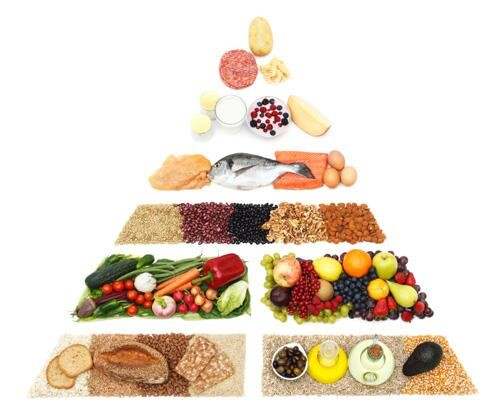
\includegraphics[width=0.6\textwidth]{img/mediterranean_diet_pyramid.jpg}
\end{center}


\textbf{Пирамида средиземноморской диеты.} Орехи – неотъемлемая часть средиземноморской диеты. Но поскольку они высококалорийные, желательно съедать в день не больше горсточки, которая помещается в одной ладони. Также средиземноморская диета содержит много бобовых. Постарайтесь постепенно вводить в свой рацион бобовые – фасоль, нут, горох, чечевицу. На их основе можно готовить супы и другие блюда.

Основной источник жиров в средиземноморской диете – это оливковое масло, которое содержит мононенасыщенные жиры. Если заменить насыщенные жиры (сливочное масло, мясо и т.п.) оливковым маслом, в организме снижается уровень «плохого» холестерина – липопротеидов низкой плотности. Лучше использовать оливковое масло, прошедшее наименьшую обработку, – «extra-virgin» и «virgin». Оно содержит максимум антиоксидантов.

Средиземноморскую диету невозможно представить без рыбы и морепродуктов. Жирная рыба (скумбрия, радужная форель, сардина, лосось, сельдь) богата на омега-3 жирные кислоты, полезные для здоровья кожи и сердечно-сосудистой системы. Средиземноморская диета предполагает умеренное употребление яиц и молочных продуктов – сыров и йогурта. Желательно выбирать продукты с низким содержанием жиров. Красное мясо появляется на столе всего лишь 1-2 раза в месяц. Это не повседневная еда, а, скорее, деликатес, которым можно себя изредка побаловать.


Некоторые научные исследования указывают на то, что умеренное употребление вина снижает риск заболеваний сердца. Но при этом важно понимать, что такое «умеренное употребление». Для женщин – это 150 мл (1 бокал) вина, а для мужчин – 300 мл (2 бокала) в день. При этом дневные дозы нельзя «накапливать». Если вы не пили всю неделю, это не означает, что на выходных можно опустошить всю бутылку.

Попробуйте средиземноморскую диету. Она не предполагает резкого ограничения килокалорий и не вызывает чувство голода. Замените красное мясо рыбой и птицей, сливочное масло – оливковым маслом, сладости – фруктами и орехами. Это простой и безопасный путь к здоровью.

\textbf{Комментарий врача Универсальной клиники «Оберіг»:} Средиземноморская диета является универсальной для профилактики и лечения большинства возрастных болезней цивилизационного мира.

Кроме общеизвестной пользы Омега-3 жирных кислот, которые содержатся преимущественно в морской рыбе, один из важнейших принципов заключается в ежедневном употреблении полезных растительных жиров, которые содержатся в оливковом масле и расширение ежедневного рациона за счет овощей, салатов.

Скажете, что данные принципы можно соблюдать только в странах Средиземноморья и только в летний период? На самом деле, в украинских традициях тоже возможна вкусная и полезная модификация. Так, Омега-3-ненасыщенные жирные кислоты содержатся также в семенах тыквы, льна, грецких орехах и арахисе, бобовых, яйцах, шпинате, капусте и мяте. В зимнее время года полезным будет употребление украинских аналогов средиземноморской диеты – свекольно-морковных салатов, овощных супов, винегрета (исключая картофель), при этом оливковое масло первого отжима можно заменить на нерафинированное подсолнечное, льняное, рапсовое, горчичное или соевое.


Соблюдение данных принципов способствует регулярной эвакуации желчи, нормализует работу желудочно-кишечного тракта, налаживает метаболизм, уменьшает уровень холестерина и риски сердечно-сосудистых осложнений.



\newpage
\section{Курение вредит вашему здоровью}
Источник: \url{https://novo-sibirsk.ru/news/266296/}

Основным веществом для табачных изделий является никотин. В равных количествах он более ядовит, чем стрихнин, и обладает в 3 раза большей токсичностью, чем мышьяк. Табачный дым в 4,5 раза токсичнее автомобильных выхлопов и в 248 раз - дыма газовой горелки.

К настоящему времени в табачных изделиях обнаружено около 4000 химических соединений, а в табачном дыме около 5000, из них около 60 веществ являются известными или предполагаемыми канцерогенами.

Смертельная доза для взрослого человека 60 мг никотина, а для детей еще меньше.

В невыкуренной сигарете содержится порядка 10 мг никотина, но через дым курильщик получает от одной сигареты порядка 3 мг никотина.

Главная опасность никотина заключается в том, что никотиновая зависимость поддерживает потребление табака. Никотиновая зависимость формируется очень быстро. Как правило, многие молодые курильщики недооценивают риск развития зависимости. Однако 98\% регулярных курильщиков, пробующих отказаться от курения, терпят неудачу сразу или начинают курить снова в течение года.

Температура табачного дыма, поступающего в рот при курении, на 35-40 градусов выше температуры воздуха и вызывает во рту довольно резкий перепад температур. Во время курения одной сигареты происходит 15-20 таких перепадов, что плохо отражается на состоянии зубной эмали: она трескается. Вот почему зубы курильщика разрушаются раньше, чем зубы некурящих.

При выкуривании 1 пачки сигарет курильщик производит около 1 грамма жидкого дегтя, который оседает на пальцах, в бронхах, легких, попадает в желудок.

Курение приводит к развитию трех основных заболеваний с летальным исходом: рак легкого; хронический бронхит и эмфизема; коронарная болезнь. 90\% онкологических заболеваний вызвано курением табака. Подсчитано, что у людей, начавших курить с 15-летнего возраста, он возникает в 5 раз чаще, чем у тех, кто закурил позже 25 лет. Продолжительность жизни курящего человека сокращается на 20-25 лет.

При выкуривании 20 сигарет в день за год курильщик получает дозу облучения, соответствующую дозе от 200 рентгеновских снимков.

У молодых курящих женщин поражаются вены нижних конечностей с последующим развитием у них эктазий, варикоза, тромбозов. Наблюдается повышенный риск возникновения ишeмической болезни сердца, инфаркта миокарда, мозгового инсульта, частота развития которого в 20 раз выше, чем у некурящих.

\newpage
\section{Вред алкоголя, его влияние на организм человека }

Источник: \url{http://pol1.tomsk.ru/novosti/281-21-09-2018}

Алкоголь – штука коварная: с одной стороны, бокал пива – просто незаменимое лекарство от перенапряжения после тяжелой рабочей недели. Но с другой – это невидимый, но достаточно ощутимый удар по здоровью, бьющий в самые уязвимые места нашего организма.

О семи причинах, почему стоит отказаться от алкогольных напитков и о том, как они способны навредить твоей жизни – далее в нашей статье.

1. Удар по сердечно-сосудистой системе. Как только алкоголь попадает в организм, сердце начинает увеличиваться в размере (особую коварность таит в себе пиво). На тканях сердца появляются многочисленные рубцы, которые являются виновниками инфаркта и способны привести к смерти.

2. Затуманенный рассудок. Алкоголь не зря считается разновидностью наркотических веществ: спиртные напитки оказывают на психику эйфорическое воздействие, продолжительность которого составляет от часа до полутора. Вскоре после этого человек впадает в депрессивное состояние, сопровождающееся агрессией и приступами панического страха. Реакции снижаются, о ясном мышлении в такой ситуации не может быть и речи. Именно по этой причине, как известно, водителям нельзя пить: вождение в нетрезвом виде может закончиться самым плачевным исходом.

3. Уничтожение клеток мозга. Даже небольшое количество алкоголя (да, полбокала вина также сюда относится) уничтожает несколько тысяч нейронов без возможности восстановления. Спирт, содержащийся в алкогольных напитках, провоцирует склеивание эритроцитов – красных кровяных телец: последние закупоривают микрокапилляры, приводя к смерти нейронов от кислородного голодания. Клетки, павшие в неравном бою с алкоголем, выводятся из организма с мочой.

4. Развитие хронических болезней. Медики приравнивают действие алкоголя к медленному яду: продукты распада спирта разрушают организм в прямом смысле слова. Человек, регулярно употребляющий спиртное, со временем все чаще начинает ощущать недомогание, его умственная и физическая активность заметно снижаются, на смену им приходит апатия. Длительная алкогольная зависимость – залог развития таких опасных хронических болезней, как панкреатит, рак поджелудочной железы, цирроз, инфаркт и масса других коварных заболеваний. Не самая обнадеживающая перспектива, не так ли?

5. Плохая наследственность. Алкоголь вносит изменения в структуру генетического кода ДНК – именно она содержит в себе информацию о человеке и его потомках. Ученые давно пришли к выводу, что 90\% детей с отклонениями в умственном развитии и врожденных инвалидов рождаются у людей, злоупотребляющих спиртными напитками.

6. Непристойное поведение. Уверены, тебе не раз приходилось наблюдать, что из себя представляет пьяный человек: алкоголь оказывает влияние на нравственные центры головного мозга, в связи с чем его дальнейшее поведение становится абсолютно непредсказуемым. В лучшем случае, все заканчивается мирным посапыванием в укромном уголке. В худшем – неконтролируемой агрессией, вспышками гнева и другими малоприятными вещами, которые в трезвом виде человек ни за что бы себе не позволил.

7. Дыра в бюджете. Цены на алкоголь (особенно хороший) немалые, и регулярное распитие любимых спиртных напитков зачастую влетает в немалую копеечку. К тому же, люди, которые начали испытывать зависимость от алкоголя, на одной бутылке не останавливаются: чем сильнее “захмелевает” голова, тем больше напитка будет куплено. Даже банальный просмотр футбольного матча практически никогда не обходится без нескольких банок пива – что уж говорить о пикнике с компанией, рыбалке или дне рождения. Если подсчитать, в какую сумму обходится такой досуг, действительно возникнет желание отложить эти деньги для более разумных целей (вложить в путешествие или же, к примеру, порадовать себя новым гаджетом).

Как видишь, существует масса причин как можно реже притрагиваться к спиртному, а то и вовсе от него отказаться. Да, алкоголь создает эффект расслабления. Да, он раскрепощает и снимает внутренние зажимы. Но тот вред, который организм получает параллельно, сводит “на нет” и без того небольшие преимущества. К тому же, расслабиться можно и другими способами – йога, плавание, горячая ванна, сауна, массаж или же неспешная прогулка в спокойном зеленом парке являются лучшими помощниками в этом деле. Позаботься о собственном здоровье сейчас, и в будущем у тебя будет в разы больше шансов избежать больничной койки и массы других малоприятных “бонусов”, нажитых за годы употребления алкоголя.

\newpage
\section{Восемь советов как избежать стресса}
Источник: \url{https://primamedia.ru/cards/health04/}

Суетливая повседневность, напряженность, проблемы, которые ежедневно нас беспокоят, нарушают наше психическое равновесие и спокойствие. Эксперты убеждены, что для эффективного управления стрессом мы должны быть достаточно мотивированы и сами выстраивать стратегию, которая поможет нам в трудные времена.

Эти советы могут быть полезны при нашем повседневном стрессе - они усилят энергию и поддержат жизненный тонус.

\textbf{1. Лестница вместо лифта.}
Когда мы пребываем в унынии, то частенько «успокаиваем» себя конфетами, сигаретой или чашечкой кофе. Гораздо лучшим вариантом является физическая активность.

В состоянии стресса или гнева попробуйте больше двигаться. Можно подняться по лестнице или совершить быструю прогулку. Даже 10 минут упражнений улучшат настроение и повысят энергетику.

\textbf{2. Еда снижает стресс. Миф! Насытьте себя «воздушной смесью».}
Вы пытаетесь снять стресс пищей? Многие считают, что это приносит комфорт, по крайней мере, в краткосрочной перспективе. Самообман.

В напряженные моменты ешьте фрукты или овощи. Это хоть предотвратит накопление лишних килограммов.

Попробуйте вместо еды, в стрессовой ситуации, сделать несколько глубоких вдохов.

\textbf{3. Полноценный сон делает нас более гармоничными.}
Качество сна – это способ борьбы с нервными состояниями. Нужно 7-9 часов сна, чтобы уменьшить стресс и подзарядиться для следующего дня.

Если у вас проблемы с засыпанием, ограничьте потребление кофеина. Избегайте тренировки за два часа до сна. Удалите из своей спальни телевизор, домашних животных, компьютер и другие «отвлекашки».

\textbf{4. Выбирайтесь из рутины.}
Даже небольшие изменения в повседневной жизни помогут улучшить настроение.

Найдите другие маршруты для похода на работу или прогулки с собакой. Измените меню завтрака или ужина.

Сосредоточьтесь на легко достижимых изменениях, чтобы добиться гарантированного успеха.

\textbf{5. Прогулка по окрестностям.}
Вам не нужно часами пыхтеть в тренажерном зале. Даже небольшие телодвижения могут быть полезны для восстановления вашей энергетики.

Простая прогулка по ближайшему скверику поможет освежить ум. Упражнения на свежем воздухе, включающие медитацию, йогу или ци-гун, помогают зарядить не только ум, но и тело.

\textbf{6. Больше волокнистой пищи!}
Получение достаточного количества клетчатки полезно для улучшения пищеварения и поддержания здоровья сердца.

Много волокон находится в овсяной муке, цельнозерновом хлебе и крупах, овощах и фруктах (в яблоках, клубнике, цитрусовых).

\textbf{7. Сосредоточьтесь на сегодняшнем дне.}  Оставьте свои мысли о прошлом или будущем, сосредоточьтесь на текущем моменте. Важно знать, где вы находитесь именно сейчас! Направьте свою энергию на то, что вы делаете в данный момент! Насладитесь тем, что с вами происходит!

\textbf{8. Не пренебрегайте здоровьем.} Мы стараемся игнорировать головную боль, «раздражающий» кашель, усталость или другие лёгкие недомогания. Но это всё влияет на наше психическое состояние, включая нашу жизнеспособность. Поэтому в случае симптомов и подозрений по поводу здоровья, рекомендуется своевременно обратиться к врачу.

Полезно внимательно слушать и уважать себя и свой организм!

\newpage
\section{Диабет}
Источник: \url{https://www.who.int/ru/news-room/fact-sheets/detail/diabetes}

\textbf{Основные факты.}
\begin{enumerate}
    \item За период с 1980 по 2014 г. количество людей, страдающих диабетом, выросло со 108 миллионов до 422 миллионов. В странах с низким и средним уровнем дохода распространенность диабета растет быстрее, чем в странах с высоким уровнем дохода.
    \item Диабет является одной из ведущих причин слепоты, почечной недостаточности, сердечных приступов, инсульта и ампутации нижних конечностей.
    \item С 2000 по 2016 г. преждевременная смертность от диабета увеличилась на 5\%.
    \item В 2019 г. диабет стал девятой ведущей причиной смерти в мире и, согласно оценкам, непосредственной причиной 1,5 миллиона случаев смерти.
    \item Здоровое питание, регулярная физическая активность, поддержание здоровой массы тела и воздержание от употребления табака могут предупредить или отсрочить возникновение диабета 2-го типа.
    \item Диабет поддается лечению, а диета, физическая активность, медикаментозное лечение и регулярный контроль и лечение осложнений помогают предупредить или задержать наступление его последствий.
\end{enumerate}

Диабет — хроническая болезнь, развивающаяся в тех случаях, когда поджелудочная железа не вырабатывает достаточно инсулина или когда организм не может эффективно использовать вырабатываемый им инсулин. Инсулин — это гормон, регулирующий уровень содержания сахара в крови. Распространенным следствием неконтролируемого диабета является гипергликемия, или повышенный уровень содержания сахара в крови, со временем приводящая к серьезному повреждению многих систем организма, особенно нервов и кровеносных сосудов.

В 2014 г. заболеваемость диабетом среди взрослого населения в возрасте 18 лет и старше составляла 8,5\%. В 2019 г. диабет стал непосредственной причиной 1,5 миллиона случаев смерти, и 48\% всех связанных с диабетом случаев смерти произошли в возрасте до 70 лет.

С 2000 по 2016 г. преждевременная (т. е. в возрасте до 70 лет) смертность от диабета увеличилась на 5\%. В странах с высоким уровнем дохода показатель преждевременной смертности от диабета снижался с 2000 по 2010 г., но затем вновь увеличился в 2010–2016 гг. В странах с уровнем дохода ниже среднего прирост преждевременной смертности от диабета имел место в оба этих периода.

По сравнению с этим, за период с 2000 по 2016 г. вероятность наступления смерти в возрасте от 30 до 70 лет по причине неинфекционных заболеваний, принадлежащих к одной из четырех основных групп (сердечно‑сосудистые, онкологические, хронические заболевания органов дыхания или диабет), снизилась во всем мире на 18\%.

\textbf{Диабет 2‑го типа.} Диабет 2‑го типа (ранее — инсулиннезависимый или диабет взрослых) развивается в результате неэффективного использования инсулина организмом. Диабетом 2‑го типа страдает более 95\% диабетиков. Данный тип диабета возникает, главным образом, на фоне избыточной массы тела и недостаточной физической активности.

Его симптомы могут быть сходными с симптомами диабета 1‑го типа, но часто менее выражены. В результате болезнь нередко диагностируется по прошествии нескольких лет после ее возникновения, уже после появления осложнений.

До недавнего времени диабет этого типа наблюдался лишь среди взрослых, однако в настоящее время он все чаще поражает и детей.

\textbf{Диабет 1‑го типа.} При диабете 1‑го типа (ранее – инсулинозависимый, юношеский или детский), для которого характерна недостаточная выработка инсулина, пациенту требуется ежедневное введение инсулина. В 2017 г. в мире было зарегистрировано 9 миллионов больных диабетом 1‑го типа, причем большинство из них проживали в странах с высоким уровнем дохода. В настоящее время причина этого типа диабета неизвестна, а меры профилактики не разработаны.

Симптомы включают чрезмерное мочеотделение (полиурия), жажду (полидипсия), постоянное чувство голода, потерю веса, нарушения зрения и усталость. Эти симптомы могут появиться внезапно.

\textbf{Гестационный диабет.} Гестационный диабет проявляется гипергликемией с показателями глюкозы крови, которые превышают нормальные, однако не достигают диагностически значимых для постановки диагноза диабета. Гестационный диабет имеет место во время беременности.

Женщинам с такой формой диабета угрожает повышенный риск осложнений во время беременности и родов. Они и, возможно, их дети подвергаются повышенному риску дальнейшего развития диабета 2‑го типа.

Чаще всего гестационный диабет диагностируется не по жалобам пациентки, а при проведении пренатального скрининга.
Снижение толерантности к глюкозе и нарушение гликемии натощак

Пониженная толерантность к глюкозе (ПТГ) и нарушение гликемии натощак (НГН) являются промежуточными состояниями между нормой и диабетом. Люди с ПТГ и НГН подвергаются высокому риску развития диабета 2‑го типа, однако этого может и не произойти.


\textbf{Последствия диабета для здоровья.}
Со временем диабет может приводить к поражению сердца, кровеносных сосудов, глаз, почек и нервов.

У взрослых людей с диабетом в 2–3 раза выше риск развития инфаркта и инсульта (1).

В сочетании со снижением кровотока невропатия (повреждение нервов) нижних конечностей повышает вероятность появления на стопах язв, инфицирования и, в конечном счете, необходимости ампутации.

Диабетическая ретинопатия, являющаяся одной из важных причин слепоты, развивается в результате долговременного накопления повреждений мелких кровеносных сосудов сетчатки. С диабетом связан почти один миллион случаев слепоты во всем мире (2).

Диабет относится к числу основных причин почечной недостаточности (3).

\textbf{Профилактика.} Известно, что простые меры по поддержанию здорового образа жизни способствуют профилактике диабета 2‑го типа либо позволяют отсрочить его возникновение. Для повышения шансов на предупреждение диабета 2‑го типа и связанных с ним осложнений, необходимо:

добиться здоровой массы тела и поддерживать ее; поддерживать физическую активность — по меньшей мере 30 минут регулярной активности умеренной интенсивности в течение большинства дней; для контроля веса необходима дополнительная активность; придерживаться здорового питания и уменьшать потребление сахара и насыщенных жиров; и не употреблять табак — курение повышает риск развития сердечно-сосудистых заболеваний.

\newpage
\section{Пять причин делать утреннюю зарядку}
Источник: \url{https://med-atlant.ru/news/5-prichin-delat-utrennyuyu-zaryadku/}

Утреннее пробуждение всегда сопряжено с сонливостью и даже некоторой ленью. Чтобы взбодриться, некоторые люди тут же заваривают себе ароматный кофе, другие начинают день с принятия душа. И только немногие пробуждаются при помощи утренней зарядки. Как показывает практика, именно те, кто взбадривает организм физкультурой, быстрее переходят в активный режим. Итак, в чем же польза зарядки? Для чего она нужна? И какие упражнения лучше делать по утрам?

Приходилось ли вам замечать, как много людей утром в плохом настроении? Врачи считают, что одна из причин такого состояния заключена в гипокинезии. Иными словами, в отсутствии физической активности. Ничего удивительного. Проработанные мышцы посылают в головной мозг достаточное количество импульсов, благодаря которым он активно настраивается на рабочий лад.

Люди, которые отказываются от утренней зарядки, часто страдают от нервной возбудимости, испытывают хроническую усталость. Они жалуются на отсутствие энергичности и бодрости утром. И только к полудню такие люди отмечают повышение активности.

\textbf{Зачем нужна зарядка.}
Организм человека не способен полностью пробудиться по звонку будильника. И даже в тот момент, когда вы уже поднялись с кровати, все внутренние органы и системы еще продолжают «отдыхать».

Во время сна замедляется циркуляция крови, затормаживается метаболизм, снижается умственная деятельность. Именно поэтому во время пробуждения человек ощущает легкую заторможенность. У него отмечается сниженная работоспособность, как физическая, так и умственная. Утром значительно ухудшена скорость реакций.

Такое состояние может длиться (в зависимости от индивидуальных особенностей) от 1 до 3 часов. Чтобы полностью проснуться и стряхнуть подобную «заторможенность», необходимо разработать суставы и мышцы. Другими словами, нужно просто сделать зарядку.

\textbf{Какая польза от зарядки?}
С самого детства родители твердили нам о необходимости делать зарядку. Лишь немногие безропотно прислушались к таким рекомендациям. А большая часть людей, прежде чем начать делать утреннюю зарядку, стремится понять, что же такого ценного она приносит.

Физическая активность в утреннее время обеспечивает следующее.

\textbf{Придает бодрость.} Организм человека просыпается значительно быстрее и активнее, если была совершена даже небольшая зарядка. После физкультуры активизируется кровообращение. Все органы и ткани начинают активно насыщаться кислородом. Ощущается прилив энергии, улучшается самочувствие. Мозг, получивший свою порцию кислорода, активно включается в рабочий процесс.


\textbf{Улучшает физическую форму.} Регулярные занятия приводят к укреплению мышечных тканей. Физкультура положительно влияет на состояние позвоночника и суставов. Даже простая и недлительная гимнастика служит отличной профилактикой развития многих болезней опорно-двигательного аппарата.

Утренняя зарядка стимулирует метаболизм. Благодаря этому человек постепенно обретает красивые формы. Некоторые мышцы подкачиваются, появляется стройность, подтягивается живот.

\textbf{Повышает настроение.} Зачем делать зарядку, если можно взбодриться от чашки кофе? Увы. Это не так. Ароматный напиток не обеспечит той энергичности и позитива, которые подарит утренняя гимнастика.

Зарядка подразумевает набор простых упражнений, которые направлены на разогрев мышц и проработку суставов. Никаких чрезмерных нагрузок утренняя физкультура не содержит. А поэтому она не вызывает ощущения усталости или боли.

\textbf{Укрепляет силу воли.}   Приняв решение делать зарядку, вам необходимо заставить себя подниматься на 10-15 минут раньше. На первых порах при правильном настрое и соответствующей мотивации вы с легкостью преодолеете этот барьер.

Но со временем, приблизительно к 20-21 дню, могут начаться серьезные трудности. Положительные результаты к этому времени еще мало заметны. Поэтому начинают появляться навязчивые мысли: «Зачем мне нужна эта зарядка, она все равно ничего не дает. Лучше поспать лишние 10-15 минут». Вот именно в этот момент важно не поддаться таким мыслям и преодолеть себя. Такое «упражнение» здорово прокачает вашу силу воли.

\textbf{Укрепляет здоровье.}
Утренняя зарядка оказывает комплексное воздействие на организм. Она активизирует кровообращение, ускоряет обмен веществ. Благодаря улучшенному кровотоку все внутренние органы получают достаточное питание и начинают значительно активнее функционировать.

Польза утренней зарядки заключена в следующих воздействиях:

\begin{itemize}
    \item укрепление сердечной мышцы;
    \item улучшение работы дыхательной системы;
    \item повышение упругости мышц;
    \item нормализация состояния сосудов, повышение их проходимости;
    \item выравнивание осанки;
    \item усиление концентрации внимания;
    \item повышение подвижности суставов;
    \item стимуляция работы мозга;
    \item повышение выносливости;
    \item нормализация работы вестибулярного аппарата.
\end{itemize}

\textbf{Утренняя зарядка: основные правила и рекомендуемые упражнения.} Существует еще одно распространенное заблуждение. Некоторые люди уверенны, что не обязательно делать зарядку утром. Можно практиковать физическую активность после обеда и даже вечером. Если речь идет об утренней зарядке, то все специалисты сходятся в одном: она должна быть утром, после пробуждения. Ведь основная цель такой гимнастики – зарядить человека бодростью и энергией на весь день.

\newpage
\section{Пять важных рекомендаций}
Источник: \url{https://med-atlant.ru/news/5-prichin-delat-utrennyuyu-zaryadku/}

Чтобы польза зарядки, выполняемой  по утрам, была максимальной, необходимо соблюдать следующие правила.

\textbf{Продолжительность гимнастикию.} Тем, кто только начинает вводить в свою жизнь утреннюю зарядку, рекомендуется планировать 10-минутную физкультуру. Со временем можно увеличить время до 15 минут. Когда организм полностью адаптируется к нагрузкам (приблизительно через 3-6 месяцев) начинайте увеличивать время зарядки до получаса.

\textbf{Подготовка к зарядке.} Не стоит приступать к гимнастике сразу после подъема с кровати. Организм еще продолжает спать. Такие нагрузки вызовут дискомфорт. Изначально нужно немного взбодриться. Для этого рекомендуется умыться, почистить зубы.

Обязательно выпейте стакан воды. Жидкость, поступившая в организм, обеспечит разжижение крови. Благодаря этому удастся нормализовать нагрузку на сердце и сосуды. А вот перекусывать перед зарядкой не стоит. Все упражнения выполняйте натощак.

\textbf{Добавьте эмоции.} Зарядка должна не только взбадривать, но и повышать настроение. Поэтому включайте любимую музыку, насыщайте воздух ароматными маслами (только не переусердствуйте) и занимайтесь гимнастикой. После физкультуры обязательно хвалите себя, отмечайте все достижения и не забывайте о поощрении.

Чтобы зарядка принесла значительную пользу для организма, предварительно проветрите помещение. Это можно сделать в то время, пока вы умываетесь. Приток свежего воздуха позволит насытить организм большим количеством кислорода.

\textbf{Регулярность занятий.} Если вы делаете зарядку от случая к случаю, то надеяться на положительные результаты не стоит. Пользу принесут только ежедневные занятия. Причем первые результаты станут заметны через 5-6 недель регулярных тренировок.

В это время люди обычно отмечают снижение уровня стресса, позитивный настрой, уменьшение возбудимости и раздражительности. Практикующие утреннюю зарядку утверждают, что к 5-6-й неделе усиливается работоспособность, повышается дисциплинированность и упорство. Люди становятся крепче и практически не подхватывают простуды.

\textbf{Правильный комплекс.} Еще один важный момент, который не следует упускать из виду, – это правильный комплекс упражнений. Гимнастика должна «запустить» все органы и ткани. Именно поэтому комплекс составляйте из упражнений, прорабатывающих все мышцы и суставы.



Утренняя зарядка должна включать в себя три этапа:
\begin{enumerate}
    \item Разминку. Ее можно делать лежа в постели. Она включает потягивание, дыхательные упражнения. В этот комплекс могут входить легкие вращательные движения кистями, стопами, конечностями.
    \item Основной комплекс. Он состоит из упражнений, прорабатывающих все мышцы и суставы. Начинают обычно с шеи, затем переходят на плечи, верхние конечности. Теперь очередь подходит к мышцам спины, живота. Заканчивают основной комплекс махами ногами.
    \item Завершение, или заминку. После основного комплекса рекомендована ходьба на месте и дыхательные упражнения.
\end{enumerate}


\newpage
\section{Рекомендуемые упражнения}
Источник: \url{https://med-atlant.ru/news/5-prichin-delat-utrennyuyu-zaryadku/}

Особое внимание следует обратить на интенсивность нагрузок. Утренняя зарядка должна приносить пользу и заряжать энергией, а не истощать организм. Именно поэтому от тяжелых упражнений (с гантелями, штангой, на выносливость и т. д.) нужно отказаться. Интенсивные тренировки лучше всего проводить после обеда. А утром отдайте предпочтение легким, простым движениям.

Утренняя зарядка обычно включает следующие группы упражнений:
\begin{enumerate}
    \item \textit{Дыхательная гимнастика}. Она улучшает работу дыхательной системы и обеспечивает активный приток кислорода к внутренним органам.
    \item \textit{Ходьба}. Очень полезно ходить босыми ногами по полу. В этом случае массируются многие активные точки. Специалисты по нетрадиционной медицине утверждают, что именно на стопе их больше всего.
    \item \textit{Гимнастика для шеи}. Она включает повороты и наклоны головы. Такие упражнения должны выполняться очень осторожно, без надрывов. Полезны вращательные движения головой. Они не только укрепляют мышцы шеи, но и тренируют вестибулярный аппарат.
    \item \textit{Физкультура для верхних конечностей}. Обязательно выполняйте упражнения на поднятие рук вверх, разведение в стороны. Вращайте конечностями. Это способствует вытягиванию позвоночника и укреплению плечевого пояса.
    \item \textit{Упражнения для кистей и пальцев}. Такие занятия полезны тем людям, работа которых связана с руками (операторы ПК, музыканты, художники, ювелиры). Эта гимнастики активизирует кровообращение и укрепляет суставы.
    \item \textit{Физкультура для поясничного отдела}. В утреннюю зарядку нужно включать наклоны в разные стороны, вперед/назад. Если нет особых проблем с позвоночником, рекомендованы упражнения на скручивания. Полезны вращательные движения талией.
    \item \textit{Приседания}. Они повышают подвижность коленных и тазовых суставов. Кроме того, такие простые упражнения позволяют улучшить внешний вид икр и бедер.
    \item \textit{Упражнения на пресс}. Если вам совершенно не дает покоя животик или очень хочется сформировать рельефные кубики на животе, то включите в зарядку упражнения на пресс.
    \item \textit{Махи ногами и руками}. Такая гимнастика повышает тонус мышечных тканей и ускоряет кровообращение.
    \item \textit{Бег, прыжки}. Эти движения отлично прорабатывают все мышцы нижних конечностей. Кроме того, они значительно усиливают метаболизм.
\end{enumerate}
Если строгие комплексы навевают на вас тоску, то можете придумать свои собственные упражнения. Главное, чтобы они не истощали вас и прорабатывали все мышцы. Кстати, никто не запрещает вам просто танцевать под любимую музыку, периодически поднимая руки, совершая махи ногами и работая талией.

\newpage
\section{Зачем нам нужны фрукты и овощи? Основы здорового питания!}
\textit{Автор: Юлия Баяндина.
    Источник: \url{https://www.shkolazhizni.ru/health/articles/63634/}}

С самого детства мы только и слышим — нужно есть свежие фрукты и овощи, в них много витаминов, они очень полезные. А почему? Этого никто не объясняет. Давайте разберемся, что нам это дает, и в чем состоит польза фруктов и овощей.

1. Поднимают настроение
Фрукты и овощи сродни шоколаду — содержат вещества (селен и фолиевую кислоту), которые способствуют выработке эндорфинов. Если что-нибудь не задалось — съешьте яблоко или банан, и настроение улучшится.

2. Дарят бодрость Фрукты и овощи содержат много воды — одновременно спасают и от голода, и от жажды, быстро усваиваются. Если нужен заряд бодрости — лучшего решения не найти. Поэтому утренний завтрак так полезно начинать с фруктов — и настроение поднимут, и энергией зарядят.

3. Добавляют витаминов Сколько фармацевты ни бьются над созданием супервитаминок, а идеального баланса найти не могут. Невозможно в одной таблетке уместить витамины так, чтобы все они полностью усваивались! С овощами и фруктами такой проблемы не возникает — все гармонично, все усваивается.

4. Помогают похудеть Овощи и фрукты содержат море клетчатки, которая почти не содержит калорий, но дает ощущение сытости. Поэтому их можно есть в любом количестве и не бояться лишнего веса — ему при таком рационе неоткуда будет взяться. Вдобавок клетчатка, словно липкая лента, собирает вредные химические вещества и канцерогены и выводит их из организма.

5. Спасают от холестерина Ничто так не страшно для сердечно-сосудистой системы, как избыток холестерина. Снизить его уровень в крови тоже помогут фрукты и овощи. Холестерин попадает в организм с животной пищей и вырабатывается печенью. В растительной пище холестерина нет, зато в ней есть пектин, который помогает выводить вредный холестерин из организма.

6. Продлевают молодость Помните молодильные яблочки из сказок? Так вот — они существуют. Сырые овощи и фрукты содержат антиоксиданты, которые помогают обновляться клеткам организма и предотвращают окисление органических соединений — попросту говоря, позволяют вам быть моложе и свежее.

7. Делают умнее Овощи и фрукты помогут сохранить ясность ума и отличную память: недавно опубликовали результаты исследования, в котором выяснили, что 6-8 фруктов и овощей в день помогают лучше запоминать и решать математические задачки. А еще фрукты и овощи спасают от заболеваний мозга: в знаменитой книге «Китайское исследование» пишут, что три порции фруктов и овощей каждый день помогут снизить риск инсульта. Одна порция -- это, к примеру, $\nicefrac{1}{2}$ чашки персиков, $\nicefrac{1}{4}$ чашки томатного соуса, $\nicefrac{1}{2}$ чашки брокколи или одна картофелина. Полчашки -- это немного.

8. Защищают от болезней Ученый Колин Кэмбелл 20 лет искал взаимосвязь между болезнями и питанием. Проверил рацион миллионов людей и доказал — фрукты и овощи лечат лучше любого доктора. Аргумент. И чем больше их в вашем рационе — тем ниже риск заболеть раком, диабетом и прочими страшными болезнями. Факт.

9. Экономят время Потому что их практически не надо готовить. Конечно, есть картофель сырым не стоит, но большинство фруктов перед едой достаточно просто вымыть. И в конце концов, фрукты и овощи — это просто очень вкусно!

% % Автор: Юлия Баяндина
% % Источник: https://www.shkolazhizni.ru/health/articles/63634/
% % © Shkolazhizni.ru

\newpage
\section{Лекарство от всех болезней, кроме смерти}
\textit{Источник: \url{https://lenta.ru/articles/2022/09/24/tmin/}}

\textit{Что говорят врачи о пользе и вреде масла черного тмина}

Семена черного тмина использовали еще в Древнем Египте три тысячи лет назад. Во время раскопок одной из гробниц археологи обнаружили бутылочку с маслом, и последующая экспертиза установила, что его изготовили из тмина. Египтяне использовали масло как один из компонентов противоядия от укусов змей, как косметическое средство и глистогонный препарат, а также употребляли в пищу для улучшения пищеварения и работы почек и печени. Как используют черный тмин и масло из него в XXI веке, «Лента.ру» разбиралась с экспертами.

Масло черного тмина имело популярностью не только в Египте. О его свойствах писали в медицинских трактатах великие древние греки Диоскорид и Гиппократ.

В арабском мире популярности масла, помимо его целебных качеств, способствовали слова, приписываемые пророку Мухаммеду. В Коране упоминается, что он называл семена тмина «лекарством от всех болезней, кроме смерти».

\textbf{Как получают масло черного тмина}

Масло черного тмина добывают путем холодного отжима семян чернушки посевной. Это однолетнее травянистое растение семейства лютиковых имеет еще несколько названий: калинджи, сейдана (седана), черный тмин, римский кориандр.

Родиной черного тмина считаются Средиземноморье и Юго-Западная Азия, где, к слову, произрастает большинство самых популярных специй. Но сейчас калинджи растет и в Крыму, и в Средней Азии, и на Балканском полуострове, и в других местностях.

Трава эта неприхотлива: всходит в степи, лесу, в садах и посевах. Черный тмин считается сорной травой, но ради семян его культивируют.

\begin{center}
    \Large
    Масло черного тмина имеет светло-желтый или зеленовато-коричневый оттенок, обладает пряным запахом и вяжущим, терпким вкусом
\end{center}

Масло черного тмина насыщено витаминами и минералами. Богатый полезными микроэлементами состав сделал его востребованным в фармакологии, кулинарии и косметологии.


\textbf{Состав масла черного тмина}

Масло черного тмина состоит из жирных кислот: арахиновой, омега-9 и омега-6, миристиновой, пальмитолеиновой и других. Если регулярно принимать масло черного тмина, то организм пополнится следующими витаминами:


\begin{itemize}
    \item витамины группы В. Оказывают положительное действие на работу ЦНС, улучшают обмен веществ, снижают риск развития анемии;
    \item витамин А. Помогает сохранять зрение, повышает защитные функции организма, улучшает обмен веществ;
    \item витамин E. Важен для сохранения беременности;
    \item витамин D. Снижает риск возникновения сердечно-сосудистых заболеваний, рахита. Укрепляет кости;
    \item аскорбиновая кислота. Повышает иммунитет, снижает уровень «плохого» \item холестерина, повышает физическую выносливость.
\end{itemize}

«Также в составе тминного масла есть каротиноиды, биофлавоноиды, фосфатидил, фитостеролы, восемь незаменимых аминокислот и важный активный компонент — тимохинон, который является мощным антиоксидантом с противовоспалительным, иммуномодулирующим и тонизирующим действием», — пояснила «Ленте.ру» терапевт клиники превентивной и антиэйдж-медицины Verba Mayr Мария Веригина.

\begin{fancyquotes}
    {\Huge 896 ккал}\\

    содержится в 100 граммах масла черного тмина
\end{fancyquotes}


\textbf{Польза масла черного тмина}

«Масло черного тмина помогает при язвенной болезни желудка, гастрите, энтерите, заболеваниях желчного пузыря и желчевыводящих путей, регулирует кислотность в желудке, — рассказала «Ленте.ру» диетолог Кристина Плотникова. — Но не стоит забывать, что это не лекарство, а сопутствующая вспомогательная терапия, и все заболевания должен лечить врач».

Масло черного тмина содержит вещества, которые могут снизить отечность, смягчить аллергические реакции, усилить иммунитет и даже отчасти помочь организму в борьбе с раковыми клетками.

Масло черного тмина имеет следующие свойства:

\begin{itemize}
    \item обезболивающее;
    \item противовоспалительное;
    \item антисептическое;
    \item бактерицидное;
    \item антивирусное;
    \item противопаразитарное;
    \item ранозаживляющее;
    \item антигрибковое;
    \item иммуностимулирующее.
\end{itemize}

\textbf{Воздействие масла черного тмина на организм}

Существует ряд исследований, доказывающих пользу масла черного тмина при лечении ряда недугов. Но стоит помнить, что его эффект пока не до конца изучен, а любая пищевая добавка не может заменить полноценного лечения под руководством опытного врача. Медики напоминают: не существует волшебной таблетки, и, если не вести здоровый образ жизни, любое средство, каким бы полезным оно ни было, не поможет справиться с последствиями вредных привычек.

\textbf{Помогает бороться с раком}

Исследования на животных показали, что семена черного тмина могут остановить рост опухолевых клеток и снизить частоту возникновения опухолей. Однако влияние на человека до конца не изучено.

\textbf{Снижает воспаление и боль при артрите}

Ученые опытным путем доказали, что микроэлементы, которые входят в состав масла черного тмина, способны улучшать состояние пациентов с ревматоидным артритом. Во время исследования части группы из 43 женщин с этим диагнозом давали масло, а остальным — плацебо. Через месяц у пациентов, принимавших масло черного тмина, зафиксировали снижение уровня маркеров воспаления крови, а также снижение интенсивности боли и уровня отека суставов.

\textbf{Защищает сердце и сосуды}

Масло черного тмина оказывает благотворное воздействие на сердце и сосуды. Оно является хорошим средством профилактики гипертонии, варикоза, тромбоза, ишемической болезни, атеросклероза.

\textbf{Помогает при аллергии}

Во время исследований в США установили, что масло черного тмина уменьшает отек в носу, заложенность носа, соответственно, помогает справиться с насморком. Правда, по данным исследования, чтобы добиться явного эффекта, масло нужно принимать две недели.

Масло черного тмина благодаря противовоспалительным и антигистаминным свойствам также способно снизить проявление аллергии и помочь быстрее избавиться от аллергического ринита.

\textbf{Избавляет от папиллом}

Бородавки и папилломы появляются на теле из-за попадания в организм вирусов. Масло черного тмина может избавить от новообразований.

Для этого нужно ватный или марлевый тампон смочить в подогретом тминном масле. Затем тампон разместить на пораженном участке кожи. Оставить его нужно на 5-6 часов, поэтому тампон следует закрепить пластырем или бинтом. Для полного избавления от бородавок и папиллом процедуру надо повторять каждый день в течение месяца.

Однако стоит помнить, что масло избавляет лишь от внешних проявлений болезни. Использовать его следует одновременно с медицинскими препаратами, назначенными врачом.

\textbf{Помогает бороться с диабетом}

Черный тмин помогает снизить уровень сахара и холестерина в крови. Люди, принимавшие добавки черного тмина, имели более низкий риск осложнений при сахарном диабете II типа. Однако это воздействие растения на организм человека предстоит изучить дополнительно.

\textbf{Поддерживает здоровье ЖКТ}

Ученые пришли к выводу, что тминное масло способно наладить процесс пищеварения и работу органов желудочно-кишечного тракта. Употребление масла помогает не только устранить причину развития заболеваний, но и убрать симптомы: приступы тошноты и рвоты, изжогу и колики.

К тому же масло тмина способствует заживлению повреждений слизистой оболочки желудка и ускорению процесса выздоровления.

\begin{fancyquotes}
    {\Huge 3-6 недель}\\

    нужно использовать тминное масло для появления ожидаемого эффекта
\end{fancyquotes}

\textbf{Помогает справиться с панкреатитом}

Принимать тминное масло можно только после наступления ремиссии заболевания и после консультации с врачом. В период обострения панкреатита масло может навредить.

После введения масла черного тмина в рацион снижается интенсивность проявления таких неприятных симптомов, как дискомфорт после приема пищи, отсутствие аппетита, метеоризм. К тому же масло останавливает размножение патогенных микроорганизмов и грибков.

\textbf{Предотвращает развитие рака простаты}

Ученые выяснили, что антиоксидант тимохинон способен подавлять рост раковых клеток в предстательной железе. Онкологи сходятся в мнении, что альтернативная медицина становится важной в качестве дополнительной терапии для больных раком, как для смягчения побочных эффектов химиотерапии, так и для усиления их противоопухолевых эффектов.

\textbf{Помогает бороться с простудой}

При простуде можно использовать масло черного тмина несколькими способами.

\begin{enumerate}
    \item Прием внутрь. Облегчить течение простуды поможет чай с тминным маслом. Но этот напиток является лишь дополнением к назначенной врачом терапии.
    \item Растирание. Грудную клетку можно растирать смесью из масла черного тмина и любого другого масла в пропорции 1:5 соответственно. Растирание поможет ослабить интенсивность кашля.
    \item Распаривание ног. Масло тмина обладает согревающим эффектом. Его добавляют в емкость с горячей водой, затем греют в ней ноги. Для большей эффективности в воду можно добавить порошок горчицы.
\end{enumerate}

\textbf{Избавляет от запора}

Тминное масло — отличное средство лечения и профилактики запоров. Оно улучшает перистальтику кишечника, размягчает каловые массы, выводит их без применения лекарственных препаратов. Особенно полезно масло как средство от запоров при беременности, во время грудного вскармливания, при нормализации стула у детей — в случаях, когда нежелательно пить лекарства.

Избежать запоров поможет масло черного тмина с чаем. Для этого нужно половину чайной ложки масла добавить в стакан чая и пить этот напиток дважды в день.

\textbf{Помогает людям с ожирением}

Масло черного тмина может помочь женщинам, страдающим ожирением. Во время исследований часть участниц научного эксперимента принимала плацебо, другая — масло. В конце исследования у участниц, принимавших масло, снизился вес, уменьшился обхват талии и уровень триглицеридов.

Исследователи также обнаружили, что сочетание диеты с приемом масла черного тмина и физическими упражнениями приводит к потере веса и снижению уровня холестерина.

Комментируя этот факт, эндокринолог клиники «РЖД-Медицина» в Твери Анна Куликова пояснила, что, согласно принципам рационального питания, следует ограничить прием всех растительных масел до столовой ложки в сутки (17 граммов). «Растительное масло, в том числе и масло черного тмина, — это на 99 процентов жир. Поэтому не стоит забывать о калорийности, ведь 100 граммов тминного масла — это почти 900 килокалорий!» — предупредила она.


\begin{fancyquotes}
    Масло черного тмина может оказывать положительное действие на организм. Входящие в его состав полезные вещества могут косвенным образом оказывать помощь в похудении. Но волшебной таблетки для избавления от лишнего веса не существует. 95-99 процентов случаев избытка массы тела связаны с перееданием и малой физической активностью.\\

    \begin{flushright}
        Анна Куликова, эндокринолог
    \end{flushright}
\end{fancyquotes}

\textbf{Облегчает состояние при астме}

Множество исследований черного тмина показали, что он облегчает состояние пациентов с бронхиальной астмой. Он оказал бронхолитическое, антигистаминное, противовоспалительное, антилейкотриеновое и иммуномодулирующее действие. Кроме того, клинические исследования установили, что при употреблении черного тмина улучшились лабораторные показатели анализов пациентов и работа легких.

\textbf{Спасает от паразитов}
Тминное масло стимулирует выработку лизоцима, способного остановить размножение глистов и других паразитов. Содержащиеся в масле элементы оказывают губительное воздействие не только на взрослых паразитов, но и их личинки.

Масло черного тмина действует следующим образом.

\begin{itemize}
    \item Убивает гельминтов, глистов, других паразитов, а также их яйца и личинки.
    \item Выводит паразитов из организма человека.
    \item Выводит из организма человека продукты жизнедеятельности паразитов — токсины.
    \item Восстанавливает пораженные паразитами ткани.
\end{itemize}

\textbf{Избавляет от геморроя}

Тминное масло входит в состав мазей и ванночек для лечения геморроя. Оно помогает снять или уменьшить болевой синдром, остановить кровотечение, упростить процесс дефекации, снять воспаление, повысить эластичность кожи и защитить ее от микротрещин.

Для избавления от геморроя нужно выпивать 2,5 миллилитра (чайная ложка) масла черного тмина утром и вечером. Но перед этим стоит проконсультироваться с врачом.

Также масло можно нанести на пораженный участок с помощью ватного тампона. Семена тмина можно добавлять в еду, смешивать с водой и медом.

[...]

% \chapter{Закон}

\section[Про Бориса Акунина]{На Бориса Акунина завели дело по двум статьям УК}

\textit{На Бориса Акунина завели дело сразу по двум статьям УК --- о «фейках» и «оправдании терроризма»}

\textit{Источник: \url{https://www.bbc.com/russian/articles/cm50vmpje43o}}

\begin{fancyquotes}
    Росфинмониторинг в понедельник внес писателя Бориса Акунина (Григория Чхартишвили) в перечень террористов и экстремистов. Следственный комитет завел на него дело по двум статьям УК. Ранее от продажи его книг стали отказываться магазины.
\end{fancyquotes}

Для \ed{фигурантов}{фигурант}{%
    person involved in; another example is В настоящее время он
    --- единственный фигурант данного дела; }
перечня государство ограничивает возможность
финансовых операций:
у попавших в список почти полностью блокируются
все банковские счета.
Они даже не могут получать зарплату и расходовать более
10 тысяч рублей\footnote{10 000 RUB = 85 GBP} в месяц.
В реестр включают людей не только приговоренных
по экстремистским и террористическим статьям УК РФ,
но и \ed{подследственных}{подследственный}{person under investigation}.

О возбуждении уголовного дела против Чхартишвили (ранее он был объявлен «иноагентом») до внесения его имени в перечень террористов и экстремистов известно не было.

Позже в понедельник Следственный комитет России сообщил, что в отношении писателя возбуждено уголовное дело о публичном оправдании терроризма и о «фейках» об армии (ст. 205.2, ст. 207.3 УК РФ). В сообщении СКР сказано, что его планируют объявить в розыск.

«\ex{Вроде бы мелкое событие}{A seemingly minor event}, запрет книг,
объявление какого-то там писателя террористом, на самом деле важная
\ex{веха}{landmark, milestone}.
Книг в России не запрещали с советских времен.
Писателей не обвиняли в терроризме со времен Большого Террора%
\footnote{«Большой террор» (\textit{разг.} «Еж\'{о}вщина»)
--- термин современной историографии, характеризующий период
наиболее массовых политических (сталинских) репрессий
в СССР 1937—1938 годов.}.
Это не дурной сон, это происходит с Россией
\ex{наяв\'{у}}{in reality}, на самом деле.
Берегите себя, не потеряйте себя, если вы в РФ.
А если вы уехали, но вам очень тяжело
\ex{на чужб\'{и}не}{in a foreign land} и вы подумываете вернуться
--- не возвращайтесь.
Ночь будет становиться черн\'{е}е и черн\'{е}е.
Но потом все-таки рассветет», ---
так прокомментировал новость сам Борис Акунин.

На прошлой неделе издательство АСТ объявило о том,
что приостанавливает распространение книг
Акунина и Дмитрия Быкова (в реестре «иноагентов»).

О прекращении продаж книг Акунина и Быкова
также объявили сеть книжных магазинов «Читай-город — Буквоед»
и сервис цифровых книг «Литрес». В «Читай-городе» решение
о приостановке продаж книг двух писателей объяснили их
«недавними \ed{высказываниями}{высказывание}{statement},
которые получили широкую огласку в СМИ».
О каких именно высказываниях идет речь, неизвестно.

\textbf{Что будет с книгами Акунина в России?}
Хранение книг Акунина пока еще остается законным,
отмечают эксперты.
Как пишет адвокат проекта «Первый отдел» Евгений Смирнов,
согласно закону о противодействии экстремистской деятельности,
запрещается распространение только тех материалов,
которые включены в реестр «экстремистских».

«Никакие книги, написанные Борисом Акуниным, а также фильмы и сериалы,
которые сняты по его романам или сценариям в этот реестр не внесены.
Если художественные произведения начнут пропадать из книжных магазинов
и стримингов --- это будет инициатива этих книжных и этих
стриминговых платформ.
Читать в метро книги о Фандорине тоже не запрещено», --- пояснил Смирнов.

\textbf{«Я помогал, помогаю и буду помогать украинцам».}
Издательство АСТ в объявлении о прекращении продаж книг
Акунина и Быкова ссылалось на «публичные заявления писателей,
которые вызвали широкий общественный резонанс».

\ex{Судя по всему}{as it appears},
имелась в виду история с провластными пранкерами Лексусом
(Алексеем Столяровым) и Вованом (Владимиром Кузнецовым),
которые обманом связались с Акуниным и Быковым и позже
опубликовали отрывки из разговоров с писателями.

Пранкеры говорили с Акуниным якобы от имени президента
Украины Владимира Зеленского и бывшего министра культуры страны
Александра Ткаченко.

В одном из отрывков, которые без контекста опубликовали
прокремлевские пранкеры, Акунин якобы говорит,
что с пониманием относится к позиции
«хороший русский --- мертвый русский».

Позже Акунин в «Фейсбуке» назвал действия пранкеров провокацией.

«Про то, что я якобы согласен с тезисом ``хороший русский
--- мертвый русский'', разумеется, \ex{брехн\'{я}}{nonsense}.
Как принято у этой шушеры, они что-то в моих словах отрезали,
что-то намухлевали, что-то \ex{перекомпоновали}{rearranged}»,
--- отметил Борис Акунин.

В разговоре с пранкерами, если судить по опубликованным отрывкам,
Акунин выразил готовность оказывать поддержку Украине.

«Я думаю, что и все другие деятели российской культуры,
которые выступают против путинской диктатуры,
с удовольствием вам помогут и примут участие»,
--- говорил, в частности, Акунин.
Эта фраза широко разошлась в соцсетях.

Писатель позже прокомментировал это высказывание так:
«Я помогал, помогаю и буду помогать украинцам».

Быков в разговоре с пранкерами произнес фразу,
возмутившую сторонников вторжения в Украину.
Ее в частности цитировало и государственное агентство ТАСС.

«Конечно, когда убивают русских, мне обидно.
Но претензий к вам у меня нет, как у меня нет претензий
к Израилю насчет Газы», — сказал писатель.

Быков и Акунин ранее неоднократно публично выступали
с осуждением российского вторжения в Украину.
Борис Акунин с 2014 года с семьей живет за границей.

Борис Акунин сам сообщал, что несколько театров
--- Российский академический молодежный театр (РАМТ)
в Москве и Александринский театр в Санкт-Петербурге
--- убрали его имя с афиш спектаклей по его произведениям.

Летом пр\'{о}шлого года издательство «Захаров» сообщило,
что московский магазин «Молодая гвардия» снял с продажи
книги писателя Бориса Акунина.
В ответ издательство отозвало из магазина все свои книги.


\newpage
\section{Запрет чайлдфри, налог на бездетность}

\textit{Запрет чайлдфри, налог на бездетность: как в России борются за рождаемость}

\textit{Источник: \url{https://news.ru/}}
% https://news.ru/vlast/zapret-chajldfri-nalog-na-bezdetnost-kak-v-rossii-boryutsya-za-rozhdaemost/

\textit{В Госдуме объявили о подготовке запрета пропаганды чайлдфри}

В Госдуме приступили к работе над законопроектом,
которым будет запрещена пропаганда чайлдфри в информационном
пространстве.
Кто и зачем хочет запретить идеологию бездетности,
запретят ли в России аборты,
каким налогом могут обложить россиян,
как власти б\'{о}рются за демографию?

\textbf{Кто хочет запретить пропаганду чайлдфри?}
О подготовке запрета на пропаганду бездетности рассказала
депутат Госдумы Ирина Филатова.
Над законопроектом работают парламентарии из нескольких
думских фракций.

«Межфракционная рабочая группа по защите традиционных ценностей
Госдумы готовит законопроект о запрете пропаганды чайлдфри.
Инициативу поддержали в ряде федеральных ведомств.
Сегодня в ограниченном формате законопроект обсуждался
на слушаниях в Общественной палате, где тоже нашел поддержку»,
--- рассказала Филатова.

Она подчеркнула, что «речь идет исключительно о деструктивной
пропаганде в информационном пространстве».

Ранее схожий законопроект разрабатывали в Башкирии с целью
защитить детей от пропаганды бездетности.
Депутаты особо подчеркивали, что инициатива не должна коснуться
вопросов бездетности по религиозным соображениям, а также книг
и фильмов о жизни монахов.

\textbf{Запретят ли в России аборты?} В марте 2023 года в Русской
православной церкви призвали ввести в России уголовное наказание
за склонение женщины к аборту в медицинских учреждениях и дополнительно
ужесточить наказания за криминальный аборт.
Депутат Госдумы Руслан Хамзаев развил эту идею,
предложив приравнять склонение к аборту к убийству человека.

Радикальные инициативы не получили немедленной поддержки,
однако к ноябрю в Мордовии, Тверской и Тамбовской областях были
введены штрафы за «склонение беременной женщины к искусственному прерыванию беременности»
--- вне зависимости от того, был произведен аборт или нет.
Патриарх Московский и всея Руси Кирилл поддержал инициативу,
но предложил расширить ее на федеральный уровень.

Член Совета Федерации Ольга Ковитиди призвала не ограничиваться
штрафами за склонение к аборту и ужесточить наказания.
Ей \ed{возразила}{возразить}{to object, to raise an objection}
глава думского комитета по правам семьи, материнства и детства
Нина Останина, призвав «прекратить организованную
\ed{травлю}{тр\'{а}вля}{bullying} врачей».
Останина ранее отмечала, что депутаты,
которые требуют запретить аборты,
ранее сами же голосовали за сокращение материнского капитала.

На региональном уровне наказания за склонение к абортам
получили поддержку: аналогичные меры в ноябре приняли и
в Калининградской области, а в декабре --- в Курской.
В ряде регионов власти сообщили, что частные клиники
в добровольном порядке прекратили проведение абортов.
О запрете процедуры, настаивают депутаты, речи не идет.

«В каждом случае все индивидуально.
У кого-то, например, есть медицинские показания.
[...] Но мы хотим ограничить наших женщин от воздействия
извне в плане пропаганды.
Речь идет, например, о какой-то явной рекламе,
например о баннерах», --- заявил курский парламентарий Юрий Амерев.

\textbf{Кто поддерживает запрет пропаганды чайлдфри?}
Против идеологии чайлдфри уже длительное время выступает депутат
Госдумы РФ Виталий Милонов. Он назвал принципиальную бездетность
«противоестественной системой ложных ценностей,
пропаганда которой не может положительно сказаться на состоянии
внутри страны».

Чайлдфри, по его словам, следует обозначить как экстремистскую
идеологию и запретить в России.

Схожее заявление сделала \ex{зампред}{deputy chairman}
Совета по правам человека Ирина Киркора,
которая усмотрела в чайлдфри «годы идеологической пропаганды»,
навязанной России.

«Безусловно, понятие ``чайлдфри'' не соотносится с теми
базовыми нравственно-духовными ценностями и категориями,
установленными в указе нашим президентом.
Вообще ``чайлдфри'' --- это не наш термин, придуман был не нами,
а, скорее, навязан уже нескольким поколениям, и он,
к сожалению, стал модным.
А к чему это приводит? Это может привести только в демографическую
\ed{яму}{яма}{pit} и в итоге к
\ed{исчезновению}{исчезновение}{disappearance} целой нации»,
--- объявила Киркора в беседе с РИА Новости.

\textbf{Как предложили ответить пропаганде чайлдфри в России?}
Ответом российских законодателей на пропаганду чайлдфри может
стать возвращение налога на бездетность.
Такой существовал в Советском Союзе и может быть введен вновь,
заявил депутат Госдумы Евгений Федоров. По мнению члена комитета
по бюджету и налогам, налог на бездетных поможет обеспечить
материнский капитал.

«Надо ли вводить налог для этого?
Если денег не будет хватать для этих проектов --- надо.
Если денег будет хватать без этого, то не надо.
Это не наказание, это способ решения проблемы»,
--- объявил Федоров.

\chapter{Энергоснабжение}
\chapter{Война и мир}

\section{Что ждет россиян во время частичной мобилизации?}
\textit{Источник: \url{https://lenta.ru/articles/2022/09/21/ukaz/}}

\textit{Ответы на главные вопросы}

Президент России Владимир Путин 21 сентября 2022 года объявил о введении в России \ed{частичной}{частичный}{partial} мобилизации. По его словам, призыву на военную службу подлежат граждане, состоящие в запасе, и прежде всего те, кто служил в армии. Кто теперь подлежит призыву, кто имеет право на \ed{отсрочку}{отсрочка}{delay; postponement}, каков порядок мобилизации — в этих вопросах разбиралась «Лента.ру».

\ed{Указ}{ук\'{а}з}{decree} «Об объявлении частичной мобилизации в Российской Федерации» опубликован на сайте Кремля в среду, в 9 часов 20 минут.

«Объявить с 21 сентября 2022 года в Российской Федерации частичную мобилизацию», — сообщается в первом пункте документа, подписанного президентом России Владимиром Путиным.

Во втором пункте указано, что мобилизованные граждане получат статус военнослужащих-контрактников с денежным содержанием соответствующего размера. Увольнение из рядов мобилизованных предусмотрено только по возрасту и по состоянию здоровья.

Правительству поручено финансировать мероприятия по проведению частичной мобилизации, главам регионов — обеспечить призыв находящихся в запасе граждан.

\textbf{Сколько человек призовут?}

Согласно заявлению главы Минобороны Сергея Шойгу — 300 тысяч. Это примерно 1,1 процента от общего мобилизационного ресурса России, который, по словам министра, составляет почти 25 миллионов человек. Для каждого региона количество подлежащих мобилизации будет определяться отдельно.

\textbf{Кого призовут в первую очередь?}

По словам Шойгу, на военную службу по мобилизации будут призваны те, кто отслужил в армии, имеет военно-учётную специальность и соответствующий опыт. Перед отправкой в части они пройдут обязательную дополнительную подготовку.

\ed{Полковник}{полковник}{colonel (army)} \explain{в отставке}{retired} Виктор Баранец считает, что первыми под мобилизацию попадут резервисты, которые каждый год по указу президента призывались на военные сборы, стреляли, водили танки и наводили ракеты. Кроме того, будут призваны люди, по разным причинам уволенные с контрактной службы, а также молодые офицеры.

«Резервисты -- это \explain{военнообязанные}{conscripts; liable for military service} граждане государства, которые подлежат мобилизации при необходимости, -- рассказал в свою очередь «Ленте.ру» \explain{судь\'{я}}{judge} в отставке Владимир Комсолев. —- В нашем случае это лица, прошедшие службу и имеющие достаточную подготовку. Они заключили контракт о пребывании в резерве и получают за это деньги. Раз в год резервисты выезжают на военные сборы, раз в месяц участвуют в занятиях».

Юрист Артем Мугунянц в разговоре с «Лентой.ру» отметил, что тех, кто пользовался отсрочкой в период с 18 до 27 лет и не служил, мобилизация, вероятно, не коснётся.

«Мобилизации подлежат только те, кто служил в армии либо офицером, либо проходил срочную службу, либо был контрактником\footnote{Only those who served in the army either as an officer, or did military service, or were a contract soldier \textit{are subject to} mobilization}. — пояснил эксперт. — Можно предполагать следующее. Так как утверждается, что необходимо освобождать территории Украины, им потребуются \explain{наступательные войска}{offensive troops}: танкисты, \explain{морская пехота}{marines}, мотострелковые части. Эти части и войска могут потребоваться в большом количестве. Тех, кто служил в этих войсках, будут мобилизовать в первую очередь».

\textbf{Людей какого возраста могут призывать?}

Согласно статье 53 Федерального закона «О воинской обязанности и военной службе», все военнослужащие запаса делятся на три разряда. В случае мобилизации первым в ВС попадает первый разряд, затем — второй, третий — последним (подробнее о том, что значат категории запаса и категории здоровья — ниже).

По первому разряду призываются солдаты и низшие \ed{чины}{чин}{rank} в возрасте до 35 лет, младшие офицеры в возрасте до 50 лет (в третьем разряде верхние рамки для этих званий повышаются до 50 и 60 лет соответственно) и так далее. Представители генералитета подлежат мобилизации по второму разряду в возрасте до 70 лет.

В Госдуме заявили, что планируют призывать тех, кто попадает под первый разряд.

«Пока человек не снят с военного учёта, он может подлежать мобилизации, — пояснил «Ленте.ру» профессор кафедры уголовного права РГПУ имени А.И. Герцена Сергей Милюков. — Есть специальности в ближнем и дальнем тылу, где возраст не является большой \ed{пом\'{е}хой}{пом\'{е}ха}{hindrance}. Например, обязательно потребуются медики. Призванные врачи будут оказывать медпомощь в госпиталях в тылу. Для лечения и \ed{дол\'{е}чивания}{дол\'{е}чивание}{follow-up treatment} нужно привлечь санатории, как это было в Великую Отечественную войну. Непосредственно же в боестолкновениях должны участвовать более молодые люди».

\textbf{Что означают категории запаса и категории здоровья в военном билете? }

Существует пять категорий годности к военной службе. Их определяют исходя из показателей здоровья и записывают данные об этом в военном билете.
\begin{itemize}
    \item «А» — \explain{годен}{fit} к военной службе;
    \item «Б» — годен к службе с \ed{незначительными}{незначительный}{insignificant} ограничениями;
    \item «В» — ограниченно годен к военной службе;
    \item «Г» — временно не годен;
    \item «Д» — не годен к несению военной службы.
\end{itemize}
Группы здоровья «А», «Б» и «В» по федеральному закону \explain{подлежат}{are subject to} мобилизации.

Всех резервистов \ed{распределяют}{распределять}{distribute} по трем категориям в зависимости от возраста военнослужащего и полученного звания.

Первая категория — граждане, которых призывают в первую очередь в случае мобилизации. \explain{Речь идет о}{This is a very useful expression; it means ``this is about...''} военных, которые не получили офицерский чин (в том числе \ed{прапорщики}{прапорщик}{ensign} и мичманы) и не \explain{перешагнули}{stepped over} возрастной \explain{пор\'{о}г}{threshold} в 35 лет, а также о младшем офицерском составе до 45 лет (лейтенант, капитан). В данной категории числятся старшие офицеры до 50 лет (майор, \explain{подполковник}{lieutenant colonel}); полковники, капитаны 1 ранга до 55 лет; высшее руководство до 60 лет. Первым на службу должен прибыть офицерский состав высшего эшелона.

Вторая категория — военнообязанные старшей возрастной группы или те, кто не прошел в первую волну мобилизации по здоровью. В эту группу попадают солдаты, военнослужащие без офицерского звания в возрасте от 35 до 45 лет, младший руководящий состав от 45 до 50 лет и старшие офицеры от 50 до 55 лет.

Третья категория — военнослужащие, которых призывают только в том случае, если военные действия длятся больше года и необходимы дополнительные силы. Под эту категорию попадают \explain{рядовые}{privates} и \explain{матросы}{sailors}, прапорщики и мичманы самой старшей возрастной категории. Возраст низшего\footnote{низкий, низшего} офицерского состава этой категории до 55 лет, а для капитанов 2 и 3 ранга и подполковников — до 60 лет. В данной категории пребывают военнообязанные женщины в возрасте до 50 лет.

\textbf{Что такое мобилизационное предписание? }

Это документ, который выдается части запасников. Выдача мобилизационного предписания — это \explain{своеобразная}{peculiar, singular, sui generis} перепись военнообязанных лиц. Гражданин, который получил мобилизационное предписание, при объявлении мобилизации должен прибыть в указанное в нем место и срок без дополнительной \ed{повестки}{повестка}{subpoena, writ} и предупреждения.

Как \explain{утверждает}{claims} юрист Павел Чиков, во время мобилизации гражданам приходят повестки, как и в обычное время — лично в руки или под подпись. Повестку также могут вручить по месту работы.

Однако именно запасники, имеющие мобилизационные предписания, по статье 21 ФЗ «О мобилизационной подготовке и мобилизации в Российской Федерации» самостоятельно должны \explain{явиться}{show up} в военный комиссариат.

\textbf{Кто имеет право на отсрочку?}

Как следует из указа, подписанного Путиным, \ed{отсрочку}{отсрочка}{postponement} пол\'{у}чат работники оборонных предприятий. «\explain{Предоставить}{provide} гражданам Российской Федерации, работающим в организациях оборонно-промышленного комплекса, право на отсрочку от призыва на военную службу по мобилизации (на период работы в этих организациях). Категории граждан Российской Федерации, которым предоставляется право на отсрочку, и порядок его предоставления определяются правительством Российской Федерации», — говорится в документе.

Как следует из статьи 18 федерального закона о мобилизации, отсрочка также предоставляется:

\begin{itemize}
    \item временно \ed{негодным}{негодный}{ineligible, not qualified} к военной службе по состоянию здоровья;

    \item ухаживающим за близкими родственниками, которых больше некому содержать;

    \item многодетным родителям (тех, кто имеет на \ed{иждивении}{иждив\'{е}ние}{dependent} не менее четырех детей в возрасте до 16 лет или троих детей при условии беременности супруги сроком не менее 22 недель);

    \item родителям-одиночкам;

    \item членам Совета Федерации и депутатам Госдумы.
\end{itemize}

Другие категории военнообязанных, которым \explain{полагается}{depends, relies} отсрочка (бронь от призыва), еще не известны. Их определяет правительство России, напомнил пресс-секретарь президента Дмитрий Песков.

\textbf{Попадают ли под мобилизацию срочники и те, кто не служил в армии? }

По закону о мобилизации — не попадают. Из него следует, что в ряды вооруженных сил должны быть направлены «граждане, пребывающие в запасе, не имеющие права на отсрочку от призыва на военную службу по мобилизации».

По словам юриста Ольги Лютницкой, \explain{срочники}{conscript} не попадают под эту категорию, так как они еще не переведены в запас.

Если гражданин не служил, например, потому, что был ограниченно годен, но у него есть военный билет, то веротность его мобилизации есть, сказала она «Ленте.ру».

Юрист Мугунянц уточнил, что срочники уже являются военнослужащими по призыву. Задействовать их до объявления полной мобилизации и войны нельзя.

\textbf{Можно ли мужчинам теперь выезжать за границу? }

В Федеральном законе «О мобилизационной подготовке и мобилизации в Российской Федерации» говорится, что «гражданам, состоящим на воинском учете, с момента объявления мобилизации воспрещается выезд с места жительства без разрешения военных комиссариатов, федеральных органов исполнительной власти, имеющих запас».

Юрист Лютницкая утверждает, что пока по вопросу \ed{запрета}{запрет}{ban, prohibition} выезда мужчинам за границу нет никаких законодательных актов и комментариев. Поэтому прямо сейчас никаких ограничений для выезда не существует.

Юрист Мугунянц также отметил, что выезжать никому не запрещено: выезд закрывается только при полной мобилизации.

«Если же человека мобилизовали, то есть признали военнослужащим, дали мобилизационное предписание о том, что он должен явиться, то он действительно не может выехать в другую страну. Потому что он мобилизован», — уточнил эксперт.

При этом скорее всего человека не будут вносить в каике-либо базы, но гражданин должен \explain{учитывать}{take into consideration}, что выезд будет расценен как \explain{уклонение}{evasion} от армии, за которое возникнут соответствующие \explain{уголовные последствия}{criminal implications}.

Член Совета по правам человека при президенте России Кирилл Кабанов заявил, что для людей без повесток на руках юридического запрета на выезд за границу нет.

\textbf{Что ждет тех, кто по достижении 27 лет получил справку вместо военного билета?}

Те, кто не проходил службу в вооруженных силах \explain{без уважительной причины}{without good reason} (например, сознательно \ed{уклонялся}{avoided, dodged}), и по достижении 27-летнего возраста получил справку \explain{взамен}{instead of} военного билета, вероятно, не будут призваны во время частичной мобилизации, так как они тоже — не служившие люди, считает юрист Мугунянц.

«На данном этапе у них никаких проблем нет. Если объявят всеобщую мобилизацию, то [обладателей справок] будут призывать, как и всех. К ним будут применяться те же условия, как к людям, которые не служили, но имеют военный билет. То же касается и тех, кто вообще не имеет никаких документов [подобного рода]. Важно, что они находятся в мобилизационном возрасте и подпадают под [всеобщую] мобилизацию».

По российскому законодательству, обладатель справки не может быть принят на государственную службу, в остальном его права не отличаются от прав владельца военного билета.

\textbf{\explain{Затрагивает}{affects} ли мобилизация женщин?}

По закону, мобилизация граждан, пребывающих в запасе, \explain{предполагает}{suggest} возможность призыва на военную службу медработников женского пола в возрасте до 45 лет. У них на руках есть военные билеты — медработники получают их после учебы.

Адвокат Владимир Шелупахин объяснил «Ленте.ру», что призыв состоящих на воинском учете женщин предполагается только в третью очередь, то есть после мужчин в возрасте 35-45 лет, в том числе граждан, пребывающих в запасе, но годных к военной службе с незначительными ограничениями (категория «Б») или ограниченно годных к военной службе (категория «В»).

«\ed{Вовсе}{вовсе}{at all} \explain{освобождаются}{released} от службы матери-одиночки и многодетные матери», — добавил юрист. Кроме того, на женщин распространяются и другие отсрочки, описанные в федеральном законе.

\textbf{Могут ли повестки приходить через «Госуслуги»?}

По официальной информации — нет. О возможной отправке повесток через сервис \ed{Госуслуг}{Госуслуги}{public services} 21 сентября написал Telegram-канала Baza. По информации издания, всем, кого собираются призвать, придет уведомление в аккаунте Госуслуг дополнением к обычным повесткам через почту.

Однако в Минцифры почти сразу это \explain{опровергли}{refuted}. «В связи с появившимися в соцсетях публикациями о том, что электронные повестки в рамках частичной мобилизации будут \explain{рассылаться}{be sent out} через Госуслуги, сообщаем, что таких планов нет. Необходимая законодательная база для этого отсутствует», — говорится в Telegram-канале министерства.

\newpage
\section{Таких замученных людей я раньше не видел}

\textit{Рассказ россиянина, который несколько суток пытался уехать в Казахстан }

\textit{Источник: \url{https://baza.io/posts/4250c126-5344-458d-af97-21179596c136}}

Сутки на жаре и холоде, драки, голод и бессонница. Со всем этим столкнулся Александр, который после объявления о «частичной мобилизации» решил уехать на машине в Казахстан. Однако там его, как и тысячи других россиян, встретил своеобразный тест на выживание и целый ряд гуманитарных проблем.

Это детальный рассказ Александра о том, что сейчас происходит на границе с Казахстаном в Астраханской области.


\textbf{Добраться до границы}

Мчались к границе под Астраханью в режиме аврала: за ночь собрали чемоданы, бросили ключи от квартиры с котом друзьям и полетели в Волгоград, так как только туда в эти дни были нормальные цены на билеты. Самолёт был полностью забит мужчинами. Когда заходил, услышал, как одна бортпроводница шепнула другой насчёт пассажирки: «О, девушка, ничего себе! Впервые за два дня».

Уже в самолёте стало ясно: ехать, как мы планировали, на поезде до Астрахани очень долго, и потому прямо в аэропорту взяли таксиста. Спросили, за сколько он довезёт до границы под Астраханью, и он, назвав сумму в 15000, сразу получил её в руки. Мы гнали больше ста весь путь. В какой-то момент водитель даже чересчур заспешил и чуть не размазал нас по встречной фуре.

Остановились только один раз — на пустынной заправке у трассы. Там был заправщик, который принялся нам угрожать и затевать драку из-за того, что мы бежим из страны. Мы ничего ему не говорили, но ему было очевидно, что мы москвичи, так как он обронил «из-за таких, как вы, у меня всех братьев забрали».

Обидно было, что он именно нас в этом обвиняет, а не власть. Но вместе с тем жалко парня: многим очевидно, что в сёлах больше пропорции набора.


\textbf{Звёзды и безысходность под Астраханью}

Подобрались к границе Астрахань — Атырау с наступлением темноты, тогда длина пробки до КПП была уже 14,9 километра. Там уже царила анархия: нам с ходу предложили купить велосипед за 50000 рублей, на котором можно было проехать границу. Далее следовал жуткий марш-бросок в кромешной тьме с чемоданами под дождём в дикий холод: вместе с тьмой на пробку опустилась осенняя прохлада и ливень.

Мы прошли вместе с чемоданами около 8 километров, разглядывая, как люди друг с другом ругаются из-за мест, как плачут уставшие дети в машинах, как кричат кошки в переносках. Люди пытались лечь спать в совершенном аду. Над нами, стоит отметить, висело фантастически красивое звёздное небо: в радиусе километров не было огней, и это был фантастический вид на звёзды. Но вместе с тем впервые пришло отчаяние: стало понятно, что выжить тут будет нереально.

Вокруг сновали люди на велосипедах с подвязанными к спине чемоданами, люди на гироскутерах, самокатах, местная банда бородатых наглецов, отжимавших места поближе к границе на продажу, и огромная, невообразимая по длине пробка из легковых и большегрузных машин, у которой не было конца. Спустя два часа такого движения, не найдя конца очереди, мы устали смертельно, и пришло понимание: либо мы сейчас едем в аэропорт и домой, либо должны немедленно устроиться на ночлег. Я был замерзший, мокрый и абсолютно раздавленный безысходностью.

И тут я увидел паренька лет 20, который ехал один в этой пробке на своей машине. Ходили слухи, что пробку на машине можно преодолеть только за сутки-полтора, и я удивился: как он в одиночку, без смены собирался ехать такой период времени без остановки? Мы предложили ему за деньги взять нас до границы, пообещав подменять за рулём для сна. Парень согласился, и мы залезли в машину. Боже, как было уютно и тепло после холодной дождливой улицы! Мы часа три-четыре ехали с ним, стараясь лавировать между дальнобойными машинами, которые пытались блокировать дорогу бомбилам, занимающим места. При этом мы весело болтали за жизнь. Стало понятно, что компания приятная.

Я чувствовал, что дико устал. Время уже было около часа ночи, как вдруг движение встало. Перед нами была вереница дальнобойщиков, уходящая в бесконечную даль, и мы в ожидании, когда вновь начнётся движение, заглушили двигатель и в какой-то момент уснули.


\textbf{«Голодные игры»}

Я проснулся спустя пару часов: было холодно даже внутри машины, хотя спал я в куртке. Парень, который нас взял, курил возле авто, закутанный во всю одежду, что у него была. Мы стояли окружённые со всех сторон дальнобойщиками, которые спали в кабинах. А вокруг был шум двигателей. Казалось, все едут, и только мы стоим в своём маленьком дальнобойном ряду.

Парень сходил на разведку и вернулся с криком «Погнали!». На часах было только 4 утра, и тьма была непроглядная. Мы очень аккуратно вылезали между дальнобойщиками на обочину и, когда выехали, увидели сцену из какого-то плохого спин-оффа фильма «Голодные игры»: сотни автомобилей носятся по полю, пытаясь обогнать друг друга в пробке на дороге и влезть где-то ближе к первому блокпосту ГИБДД.

Мы вместе со всеми выехали на поле и оказались в абсолютной мясорубке: ночь, вой моторов и сотни водителей, выдавливающих друг друга с дороги в кювет. Уже не знаю, как у паренька это вышло, но благодаря своей наглости и терпению он нашёл небольшой перекрёсток с просёлочной дорогой, чтобы вклиниться, и мы заняли позицию до рассвета.


Рассвело к шести, и на перекрёстке появился сотрудник ГИБДД. Он пытался разрулить весь тот кошмар, который произошёл за предрассветные часы. Водителей, ждущих в пробке уже сутки, это злило: кто-то за ночь влез без очереди из-за дальнобойщиков, которые заблокировали поток в знак отместки за потерянное время. Теперь такие водители не давали сотруднику ГИБДД пропускать влезшие с обочины машины.

Инспектор был абсолютно уставший и измождённый и в какой-то момент просто ушёл, оставив всё это дело жить своей жизнью. А жизнь была такая: пока на горке совершали намаз мусульмане, семьи с детьми пытались умыть уставших и невыспавшихся детей, а кто-то гулял с собакой, привезённой с собой в этот кошмар.

«Нам тут не влезть», — хмуро сказал наш водитель, и мы пошли искать сообщников на прорыв. Картина открывалась жуткая. Поговорив с окружающими, мы узнали, что люди, стоявшие в честной пробке, провели здесь уже сутки, тогда как наш маршрут занимал около 10 часов. Многие были с детьми, пожилыми родителями, животными. Кто-то из них набрал попутчиков. Но всех объединяло одно: все они, так же как и мы, ночью были заблокированы колонной дальнобойщиков.

Услышав шум машин и оскорбившись такой наглостью, водители бросились объезжать их по полям, перемешивая все очередности. Этот перекрёсток был всего в 5 километрах от границы.


\textbf{Банка майонеза, драки и ФСБ}

В пробке было много машин с Северного Кавказа: с номерами из Дагестана, Чечни, Ингушетии. Они везли семьи, детей, родителей: их семьям угрожало наказание за то, что они уклоняются от мобилизации, потому всех брали с собой. Здесь же были и напуганные студенты, и взрослые мужчины, и ребята со всей страны: Ростовской, Краснодарской областей, попадался Санкт-Петербург и Карелия. Представьте, люди приехали сюда из Карелии!

Куда, спрашиваю у водителя, здесь ходят в туалет? Он смеется: «А как ты думаешь? Спустись с дороги». И тут я увидел страшное зрелище: отходить от дороги далеко нельзя — вдруг твоё место займут? Тех, кто ушёл дальше 50 метров, разворачивали пограничники. Поэтому люди были вынуждены ходить в туалет прямо здесь, на глазах всей пробки. Десятки тысяч людей, женщин, мужчин, любых вероисповеданий и культур. Все делали это здесь.

Обстановка накалялась: люди не могли поделить дорогу, и вспыхивали драки в разных частях пробки. Солнце окончательно поднялось, и стало жарко. Ещё ночью ты заворачивался во все вещи из чемодана, а сейчас потел в футболке.

Стало понятно, куда уехал сотрудник ГИБДД: он вернулся с группой пограничников и бойцами ФСБ на «Барсе». Они подняли оружие, будто угрожая начать пальбу в воздух, но толпу это мало пугало: несколько ретивых ребят попытались втянуть в драку инспектора. Только с появлением майора ГИБДД — уставшего, с выгоревшей на солнце кожей и грозным голосом — удалось сбить накал и договориться о системе проезда. Разумеется, и она не соблюдалась. Как только инспектор принимался разруливать проблему в одной точке пробки, вспыхивали бои в другой.

Мы смогли въехать на точку, указываемую в многотысячных чатах пробки как ключевую, после которой «ад заканчивается» и «всё становится интеллигентно». Здесь находился узкий мост, и далее авто двигались в образовавшейся колонне одна за другой. Ну как двигались: за 12 часов все продвинулись на 600–700 метров, не более.

Тут появилась гуманитарная проблема: у кого-то заканчивалось топливо, у кого-то еда и вода для детей и взрослых. Некоторые были отправлены в город за едой, но тут же попадали в капкан: их машины не хотели пропускать обратно в задней части пробки, и эти машины выбывали из общей гонки.

К этому времени о пробке уже трубили СМИ. Новости от тех, кто был на границе, расстраивали: они стояли по трое суток. Мы достигли посёлка, в конце которого находился КПП, только к темноте. В посёлке в это время совершенно опустел магазин: только одинокая банка майонеза стояла в пустом холодильнике. Проблема с водой, едой и топливом решена не была: люди в моей части колонны делились этим с соседями, некоторые продолжали толкать машину, чтобы не заводить авто и не тратить топливо. Я отдал две из трёх оставшихся бутылок воды в соседние машины с детьми, а также раздал большую часть своей аптечки. Особенно было популярно обезболивающее.


Обочина в этой части была полна мусора от наших предшественников, а также сбежавшимися на него собаками. Это отпугивало людей от туалета. Еда почти у всех кончилась, наступила ночь, и снова стало холодать.

На помощь пришли жители посёлка. Они за крайне низкие цены стали продавать еду, заряжать телефоны, бесплатно пускать в туалет, а детей — отдохнуть в дома. Но вместе с темнотой пришла и новая проблема: организованные «мафиози» держателей мест вклинивались в ряды. Их целью было удержать позицию в этой части пробки и продать их тем, кто прибыл в конец.

По слухам, место в этой части пробки стоило по 25–30 тысяч рублей. Это приводило к конфликтам и дракам, маханию ножами и угрозам убийством. На самые громкие драки прилетали сотрудники ФСБ на «Барсе», в балаклавах и с автоматами. Это успокаивало конфликтующих — до отъезда офицеров.


\textbf{Дорожная «мафия»}

Здесь, в 4 километрах от границы, уже было много пешеходов с сумками. Они доходили до этой части колонны и просились в машины: переходить границу пешком было нельзя. У обочины были свалены велосипеды: люди, накупившие их в конце пробки за 30–50 тысяч рублей, у КПП узнавали, что на велосипеде было всё-таки нельзя. Пеших кто-то подсаживал бесплатно, а кто-то брал за деньги. И тут начался новый коллапс: каждый, кто слышал о более высокой цене, поднимал цену у себя, и в итоге стоимость места в машине выросла до 40–50 тысяч рублей.

Чем темнее становилось, тем активнее начинались бои во второй части «Голодных игр». Вместе с этим накопилась усталость: за двое суток, из которых на сон пришлось 3 часа, мы не выспались. Первоначальный план, согласно которому мы хотели меняться местами с водителем, разбился о необходимость вылетать из машин по свисту — для обороны мест от влезавших барыг-продавцов. Это длилось всю ночь.

Третьи сутки прошли по абсолютно такому же сценарию, но изменились цены: мы были уже в 2 километрах от КПП, и цены на места для пассажиров достигали 70 тысяч. Еда и вода стали дефицитными, мы совсем отказались от еды в пользу детей, водой нас снабжали местные жители совершенно бесплатно. Для экономии топлива многие стали толкать машины. Чтобы хоть как-то спать, часть не умеющих водить пассажиров освоили основы вождения.

К ночи началась третья серия «Голодных игр» с ещё более активным противостоянием. Здесь уже оставалось менее 500 метров до КПП, и дорога была блокирована десятками мужчин, утверждавших, что это их территория, а машины будут пропускаться по системе «шесть из колонны — одна их».


«Одна их» представляла собой минивэн с вместимостью 6–12 человек, куда сажали пешеходов по цене от 70 до 90 тысяч рублей за место. На дороге появились «служебные машины» с сопровождением ГИБДД, следовавшие в сторону КПП. В числе служащих были замечены пожилые женщины и подростки. Обратно они не возвращались.

Бои длились до утра. Под эффектный рассвет мы пересекли КПП. Там все уже были знакомы: сотрудники ФСБ, помогавшие отвоёвывать места, пограничники, с уставшими лицами проезжавшие мимо пробки на микроавтобусе, работники ГИБДД, нервно курившие после изнуряющей смены в ночном кошмаре.

На КПП были и молодые люди, которых задержали в связи с тем, что они получили повестки. Стало ясно, что слухи о списках на границах вовсе не были слухами.


\textbf{Переход}

Под встающее солнце мы с уже родными соседями пересекали границу и неслись по буферной зоне, в которой, как нам завещали сотрудники российской погранзаставы, не стоит покидать автомобиль. Проехав шесть километров из двенадцати, мы уткнулись в новую пробку.

У буферной зоны была особенность: здесь не было ни сотрудников ГИБДД, ни ФСБ. Зато были свои барыги: они перевозили людей за 30–50 тысяч от одного КПП до другого через встречную полосу. Здесь они были более подготовлены и ездили по двое, с охраной. Но и люди, попавшие в эту зону, были уже ветеранами и прямо между двумя погранзаставами мастерили себе примитивное оружие близкого боя. Как ни странно, боёв не было. Но день прошёл в столкновениях и наездах машин барыг на активистов пробки.

Моторы здесь не заводились, даже для движения в горку, пить воду перестали даже женщины, кто-то набирал воду из местной реки, которая оказалась достаточно чистой. Не было слёз и истерик: к четвёртым суткам погранперехода плакать уже не умели, лишь сурово грустить. Я был знаком с людьми на десятки машин назад и вперёд: отличные ребята со всей европейской части страны, бегущие от правительства и безысходности.

Организовывались сигналы тревоги и группы быстрого реагирования для непропуска барыг. Дальнобойщики, чудом прорвавшиеся в эту зону, грели воду для бытовых нужд: некоторые впервые за эти дни чистили зубы или умывались. На реке появилась лодка: в ней приплыла семья из республики Северного Кавказа, пересекшая таким образом границу: они бесплатно раздавали всем еду, воду и лекарства.

К ночи приехали российские пограничники. Они строго запретили покидать автомобили: таковы были правила проезда. Исключения сделаны были для тех, кто толкает машины. К глубокой темноте мы прошли мост — переход через границу и встали в очередь к казахскому КПП.

Последний этап этого квеста был связан с полным отсутствием сил. Без еды, сна и покоя мы провели по четверо суток. Впереди было ещё шесть часов в пробке. Появился интернет, а вместе с ним в чате пробки появилась информация о местах в машине по 150000 рублей и барыгах, которые перевозили людей в нейтральную буферную зону за одну сумму, а уже в буферной зоне требовали другую. Те, кто не соглашался, отправлялись обратно.

Водители засыпали за рулём: сказывались по 80–96 часов без отдыха. Все были измождены и глубоко несчастны. Казахские пограничники встречали людей сочувствием и крайне лояльным досмотром. Впервые показалось, что мы действительно беженцы: таких несчастных и замученных людей я раньше не видел.

Впереди у нас было ещё шесть часов по бездорожью в степи до ближайшего города.


\newpage
\section{Народ — президент — Бог}


\textit{Зачем «военное духовенство» РПЦ заменяет Евангелие Ветхим Заветом, а \explain{з\'{а}поведь}{commandment} о любви — заповедью об уничтожении врагов }

\textit{Александр Солдатов, обозреватель «Новой газеты»}

\textit{Источник: \url{https://novaya-media.cdn.ampproject.org/}}

Православный федеральный телеканал «Спас» выпустил цикл передач «Война и Библия». Главный редактор телеканала Борис Корчевников в сопровождении настоятеля храма РПЦ при МГИМО протоиерея Игоря Фомина, позируя в полной военной экипировке, продвигают такую трактовку библейских сюжетов, которая, по их мнению, полностью объясняет происходящее. Вышло уже пять серий цикла, основной набор идей повторяется в каждой из них: «СВО» имеет сакрально-мистический характер; на стороне Украины сражаются еретики и сатанисты, а российская армия исполняет заповеди, данные еврейскому народу при исходе из Египта, когда он покорял Палестину — Землю обетованную, истребляя населявшие ее народы.

Мистический крен в российской пропаганде возник в октябре — на фоне кризиса первоначальных целей «спецоперации» («демилитаризация» и «денацификация») и усилился на фоне частичной мобилизации. Хотя религиозность россиян (особенно мужского населения) не очень высока, власть вынуждена обращаться к религиозной риторике — с ее помощью формируется некая синкретическая религия, которая игнорирует различия, например, между православием и исламом, акцентируя внимание на «духовной несовместимости» Запада и России.

Представляя основные постулаты этой религии, помощник Николая Патрушева Алексей Павлов заявил: «С продолжением специальной военной операции становится все более насущным проведение десатанизации Украины, или, как метко выразился глава Чеченской Республики Рамзан Кадыров, ее «полной дешайтанизации».

Развивая этот тренд, Дмитрий Медведев наделил РФ, олицетворяемую президентом, божественными свойствами: «Мы приобрели сакральную силу, — заявил он. — У нас есть возможность отправить всех врагов в геенну огненную». И сформулировал новую цель «СВО»: «Остановить верховного властелина ада, какое бы имя он ни использовал — Сатана, Люцифер или иблис».

\begin{fancyquotes}
    Медведев угрожает украинцам словами из ветхозаветного пророчества Иезекииля: «Не пощадит тебя око Мое, и не помилую. По путям твоим воздам тебе, и мерзости твои с тобою будут; и узнаете, что Я Господь каратель» (Иез. 7:9).
\end{fancyquotes}

В отличие от Евангелия, которое, как утверждает Коран (2:75; 4:46; 5:13, 41), христиане «исказили», Ветхий Завет — священные книги еврейского народа, написанные до пришествия в мир Христа, — равно почитаются христианами и мусульманами. В исламской традиции они известны как «ат-Таурат». В этом контексте неудивительно, что авторы цикла «Война и Библия» апеллируют именно к Ветхому Завету. В 4-й серии они смакуют историю истребления семи народов при завоевании Палестины еврейским воинством под предводительством Иисуса Навина.

Ведущий Борис Корчевников называет заповедь «Пойди и вырежи весь народ» великим испытанием веры. А протоиерей Игорь Фомин ополчается на либералов, которые считают, что «даже правитель не может лишать жизни». «Но Священное Писание, — утверждает воинствующий служитель, — говорит совершенно об обратном».

Подмена тут заключается в том, что христиане имеют другое Писание! Точнее, ключом для понимания Писания у христиан служит Евангелие, а у православных — еще и тысячелетняя святоотеческая традиция его толкования. Иисус Христос в Евангелии часто цитирует заповеди Ветхого Завета, но почти каждый раз предлагает совершенно новое, духовное их понимание. Вспомним Нагорную проповедь: «Сказано древним: не убивай, кто же убьет, подлежит суду. А Я говорю вам, что всякий, гневающийся на брата своего напрасно, подлежит суду… Сказано древним: не \ed{прелюбодействуй}{прелюбодействовать/спрелюбодействовать}{to commit adultery}. А Я говорю вам, что всякий, кто смотрит на женщину с \ed{вожделением}{вожделение}{страстное желание; сильное чувственное влечение (lust)}, уже прелюбодействовал с нею в сердце своем\dots Сказано: око за око и зуб за зуб. А Я говорю вам: не противься злому. Но кто ударит тебя в правую щеку твою, обрати к нему и другую… Сказано: люби ближнего твоего и ненавидь врага твоего. А Я говорю вам: любите врагов ваших, благословляйте проклинающих вас, благотворите ненавидящим вас и молитесь за обижающих вас и гонящих вас» (Евангелие от Матфея, глава 5).


\begin{fancyquotes}
    Евангелие — самая неудобная книга в современных реалиях.
\end{fancyquotes}

Встречаясь с военным духовенством 1 декабря в храме Христа Спасителя, патриарх Кирилл также не цитировал эту неудобную книгу. Он \ed{восхвалял}{восхвал\'{я}ть/восхвал\'{и}ть}{to praise} \ex{доблесть}{\textit{высок.} высшая добродетель (virtue); стойкость; высшее мужество, готовность преодолеть препятствия для достижения какой-либо высокой цели, самоотверженность в какой-либо деятельности} тех, кто «с оружием в руках защищает родину», и выражал надежду, что поездки духовенства на фронт «закалят» священников. Патриарх намерен «циркулярными письмами» направлять туда все новые и новые партии духовенства. В своей потрясшей христианский мир проповеди 25 сентября он автоматом признал попавшими в рай всех российских воинов, погибших на полях Украины: по его мнению, такая гибель «смывает все грехи, которые человек совершил».

\begin{fancyquotes}
    «Идите смело исполнять свой воинский долг, — напутствовал Кирилл воинов. — Если вы жизнь положили за родину ``\dots'', то вы будете вместе с Богом в Его Царствии».
    Евангелие содержит совсем другие «напутствия воинам».
\end{fancyquotes}

«Возврати меч твой в его место, ибо все, взявшие меч, мечом погибнут» (Мф. 26:52), — говорит Христос апостолу Петру, пытавшемуся защитить Учителя от ареста (об истории толкования этого места Евангелия рассказывала «Новая»). «Наша война не живых делает мертвыми, а мертвых — живыми, изобилуя \ed{кротостью}{кротость}{свойство по значению прилагательного кроткий; добродетель, заключающаяся в уклонении от проявления гнева и ярости; уступчивость, покорность, смиренность (meekness)} и великим смирением, -- говорил святитель IV в. Иоанн Златоуст о духовном понимании ветхозаветных сюжетов о войне (\url{https://religion.wikireading.ru/amp190553}). — \ed{Мне привычно}{мне привычно}{I'm used to} терпеть \ex{преследование}{pursuit}, а не преследовать, быть гонимым, а не гнать. Так и Христос побеждал, не распиная, а распятый, не ударяя, но приняв удары».

«Народ — президент — Бог», --- торжественно декламирует новую русскую «триаду» протоиерей Игорь Фомин. Она рефреном \ex{пронизывает}{pervades} цикл «Война и Библия», апеллируя прямо к подсознанию зрителей, убеждая в том, что все три реальности вечны и бессмысленно возражать или сопротивляться им. Главный посыл этих грубых намёков --- президент \ed{непогрешим}{непогрешимый}{не совершающий ошибок, не ошибающийся (infallible)}, даже если большинству его подданных непонятен смысл самого важного решения всей его жизни, а может быть, и всей истории России. Народ призывают не искать рациональных объяснений происходящего, а экстатически \ed{восклицать}{восклиц\'{а}ть/воскл\'{и}кнуть}{громко говорить что-либо, выкрикивать} вслед за Тертуллианом: «Credo quia absrdum est!» (Верую, ибо абсурдно!).


\newpage
\section{Американский профессор назвал цель визита Байдена в Великобританию}

\textit{Источник: \url{https://lenta.ru/news/2023/07/07/visit_biden/}}

\textit{Профессор Кузник: Байден встретится с Сунаком в Лондоне для обсуждения поставок Украине}

Цель визита президента США Джо Байдена Лондон не только укрепление отношений между странами, но также обсуждение поставок вооружений Украине. Об этом сообщили «Известиям» американские эксперты.

Как отметил профессор кафедры истории Американского университета в Вашингтоне Питер Кузник, в руководстве европейских стран в настоящее время наблюдается некоторое «отклонение от курса». Кроме того, растет давление со стороны Организации объединенных наций (ООН), Ватикана и Глобального Юга, выступающих в пользу начала переговоров.

Кузник подчеркнул, что в ходе визита в Лондон американский лидер встретится с премьер-министром Великобритании Риши Сунаком, который является «одним из самых \ed{ярых}{ярый}{ardent} милитаристов в НАТО». Ожидается, что лидеры стран обсудят дополнительные системы вооружения для Украины, включая поставку истребителей F-16. Также эксперт допустил, что Байден и Сунак затронут вопрос поставок Киеву оперативно-тактических ракетных комплексов ATACMS. В то же время Кузник выразил мнение, что это не повлияет на исход украинского контрнаступления.

Ранее стало известно, что с 9 по 13 июля Байден посетит Великобританию, Литву и Финляндию. В Вильнюсе американский лидер планирует принять участие в 74-м саммите НАТО.

\newpage
\section{Китайские и турецкие ЧВК пришли воевать в Африку}

\textit{Источник: \url{https://lenta.ru/articles/2023/07/06/pmc_wagner/}}

\textit{Смогут ли они занять место ЧВК «Вагнер»?}

\textit{«Лента.ру»: китайские и турецкие ЧВК не смогут занять место «Вагнера» в Африке}

До неудачной попытки вооруженного мятежа частная военная компания (ЧВК) «Вагнер» не только была активно вовлечена в боевые действия на Украине, но и помогала правительствам нескольких африканских стран в борьбе с повстанцами и террористическими группировками. И если про первое понятно, что бойцы ЧВК смогут продолжить участие в конфликте, лишь подписав договоры с Министерством обороны России, то в ситуации с Африкой по-прежнему остается немало вопросов. Вместе с тем на протяжении последних лет наблюдатели отмечают растущую на континенте активность частных охранных и военных компаний из Китая и Турции. «Лента.ру» разобралась, какая судьба ждет \ed{подразделения}{подразделение}{division} ЧВК «Вагнер» в Африке и почему их место могут занять китайские и турецкие \explain{наемники}{mercenaries}.

\textbf{Уйти нельзя остаться.} Вскоре после мятежа Евгения Пригожина в американских СМИ появились сообщения о панике среди руководства Центральноафриканской Республики (ЦАР). По информации The Daily Beast, в Банги испугались, что мятеж может привести к сворачиванию африканских подразделений ЧВК «Вагнер», которые с марта 2018 года помогали местным властям в борьбе с \ed{повст\'{а}нцами}{повст\'{а}нец}{rebel}.


\begin{wrapfigure}{l}{0.5\textwidth}
    \begin{fancyquotes}
        Русские играют очень важную роль в архитектуре безопасности нашей страны, и, если они будут вынуждены полностью прекратить свою деятельность, все может \ex{пойти наперекосяк}{go awry}\\

        \begin{flushright}
            на условиях анонимности специально\\

            для The Daily Beast
        \end{flushright}
    \end{fancyquotes}
\end{wrapfigure}
Туманным остаются перспективы подразделений ЧВК «Вагнер» и в других африканских стр\'{а}нах, например в Мали, куда «музыканты» пришли осенью-зимой 2021 года. Несколькими месяцами ранее, в июне 2021 года, президент Франции Эммануэль Макрон объявил о выводе из западноафриканского государства французских военных, с 2013 года помогавших в борьбе с террористами из местных франшиз «Аль-Каиды» и «Исламского государства» (террористические организации, запрещённые в России). Образовавшуюся «пустоту» власти Мали решили заполнить ЧВК «Вагнер».

\begin{figure}[h]
    \centering
    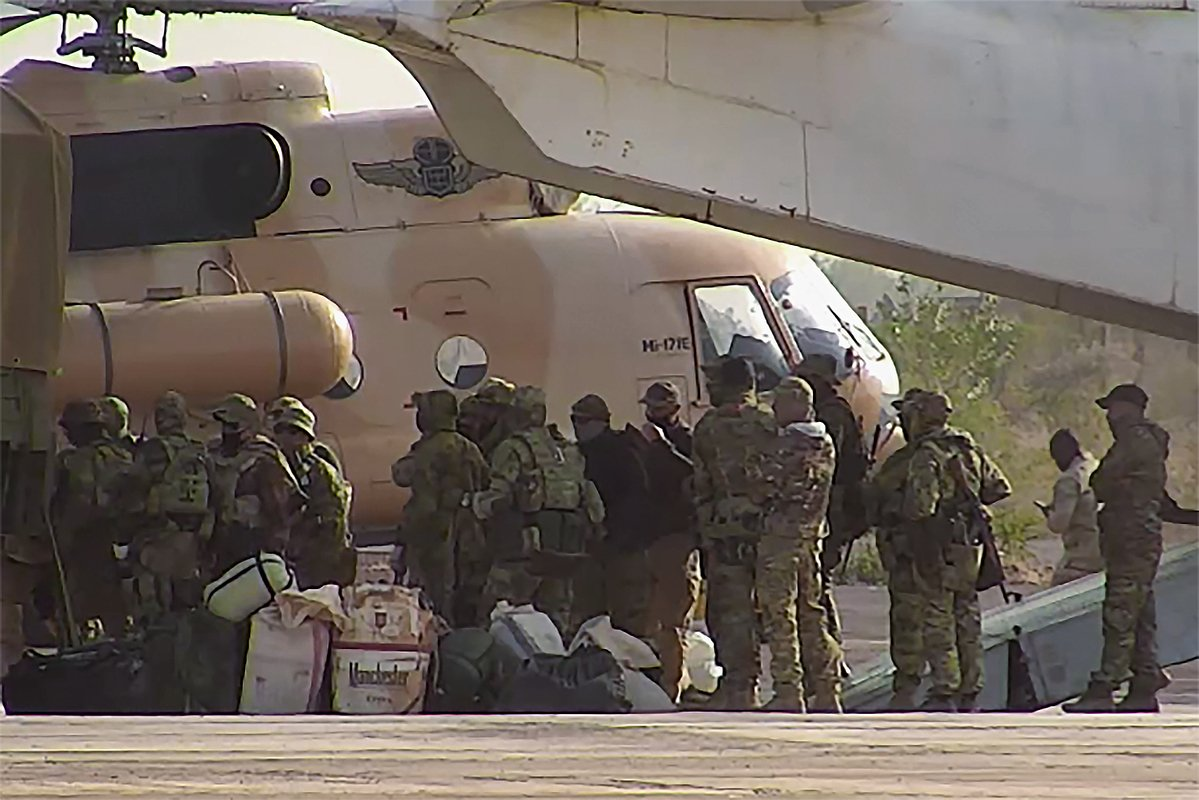
\includegraphics[width=0.75\textwidth]{img/pmc_africa_1.jpg}
    \caption{Предположительно сотрудники ЧВК «Вагнер» садятся в вертолет на севере Мали, фотография не датирована; Фото: French Army / AP}
\end{figure}

Также сообщалось, что за услугами «музыкантов» обращались различные политические силы в Ливии, Судане, Мозамбике, а также, возможно, власти Буркина-Фасо (хотя они это отрицают). По разным данным, в обмен структуры ЧВК «Вагнер», помимо финансового \ed{вознаграждения}{вознаграждение}{remuneration; compensation}, также получали доступ к добыче природных ресурсов в странах пребывания.

\begin{center}
    \Large

    Впрочем, министр иностранных дел России Сергей Лавров \ex{заверил}{reassured}, что никакой паники среди африканских коллег не заметил
\end{center}

Напротив, ряд африканских представителей связались с ним, чтобы выразить свою солидарность с российским руководством. По его словам, правительства Мали и ЦАР, помимо пригожинской ЧВК, поддерживают контакты с официальными властями, а несколько сотен военнослужащих, которые работают в ЦАР в качестве инструкторов, продолжат свою работу, несмотря на последние события.

При этом официальный представитель Министерства иностранных дел (МИД) России Мария Захарова уточнила, что решение о продолжении работы в Африке непосредственно специалистов ЧВК «Вагнер» будут принимать сами африканские страны. Также она подчеркнула необходимость отделять обычных бойцов от организаторов мятежа, призвав «смотреть не на trademark ``Вагнер'', не на термин, а на суть».

\begin{wrapfigure}{r}{0.5\textwidth}
    \begin{fancyquotes}
        Она заключается в том, что за последние годы люди это доказали, занимаясь на фронте, на передовой, обеспечением нашей безопасности (...) проявляли себя соответствующим образом в Сирии, в африканских государствах

        \begin{flushright}

            Мария Захарова\\

            пресс-секретарь МИД России
        \end{flushright}
    \end{fancyquotes}
\end{wrapfigure}
Однако непонятно, позволят ли бойцам оставаться в Африке под тем самым trademark «Вагнер». В своем обращении президент России Владимир Путин дал «музыкантам» выбор из трех вариантов: заключить контракт с Министерством обороны России или другим силовым органом, вернуться домой к родным или «уйти в Белоруссию».


\begin{center}
    \Large
    \ed{Затрагивают}{затрагивают}{affect} или нет эти слова и тех бойцов ЧВК «Вагнер», что находятся в Мали и ЦАР, непонятно
\end{center}


\begin{figure}[h]
    \centering
    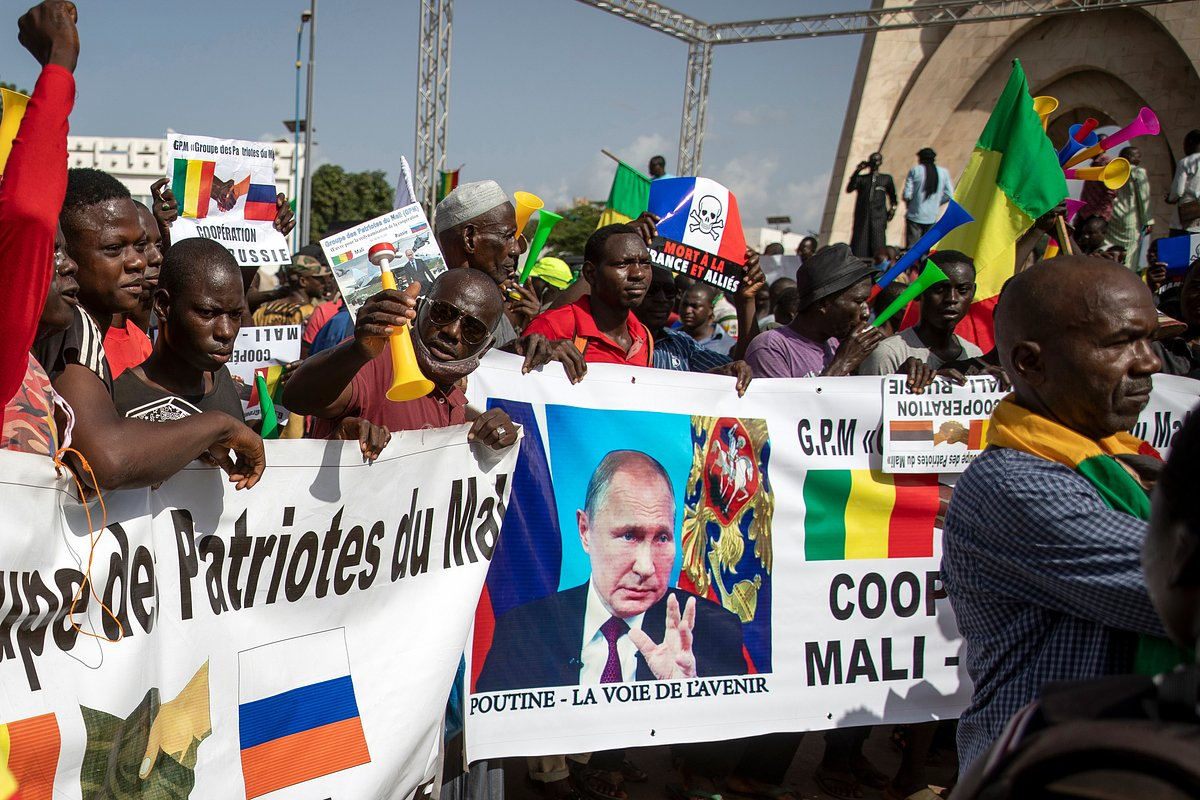
\includegraphics[width=0.75\textwidth]{img/pmc_africa_2.jpg}
    \caption{Жители Мали на демонстрации против Франции и в поддержку России по случаю 60-летия независимости страны, Бамако, 22 сентября 2020 года; Фото: AP }
\end{figure}

Более того, глава комитета Государственной Думы по обороне Андрей Картаполов заявил: отказавшиеся от подписания договоров формирования не будут получать «ни денег, ни финансовых, ни материальных ресурсов». Как отмечает The Financial Times, без материальной и логистической поддержки российских властей вагнеровцам будет крайне сложно продолжить работать в Африке.

\begin{center}
    {\Huge 86,3}\\
    {\huge млрд рублей}\\[1em]

    {\Large выплачено ЧВК «Вагнер» из госбюджета с мая 2022 года по май 2023 года }
\end{center}

«Лента.ру» направила запрос в пресс-службу Министерства обороны России с просьбой прояснить позицию ведомства по данному вопросу. На момент публикации материала ответа не поступило.

\begin{center}
    \Large Сам Евгений Пригожин не рассказывал, чем дальше будет заниматься его ЧВК «Вагнер» и сохранится ли ее африканское подразделение
\end{center}


\begin{figure}[h]
    \centering
    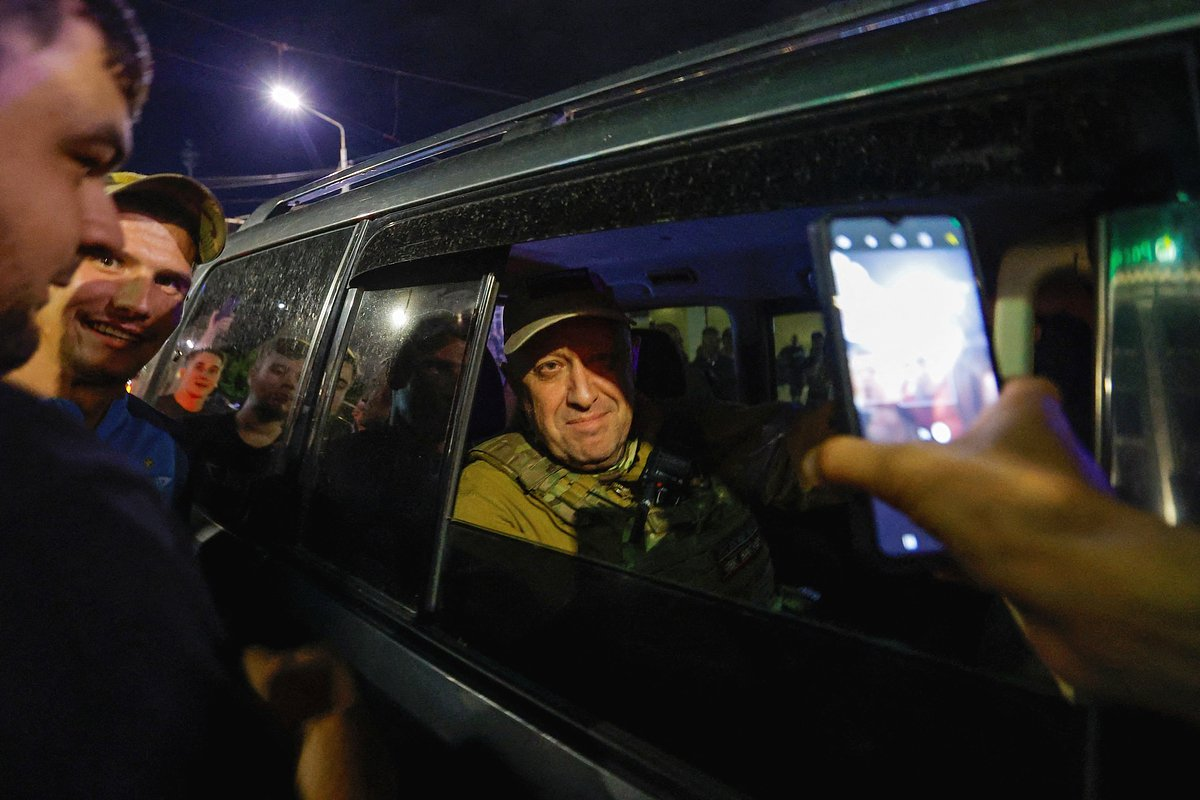
\includegraphics[width=0.75\textwidth]{img/pmc_africa_3.jpg}
    \caption{Евгений Пригожин покидает штаб Южного военного округа в Ростове-на-Дону, 24 июня 2023 года; Фото: Alexander Ermochenko / Reuters}
\end{figure}

Президент Белоруссии Александр Лукашенко, выступивший в качестве посредника между российскими властями и Евгением Пригожиным, заявил, что ушедшие в республику вагнеровцы могут быть привлечены к обучению местных подразделений.

Впрочем, пока дипломаты в ЦАР не заметили очевидных перемен в обстановке в стране после мятежа: представители ЧВК «Вагнер» были замечены в Банги и после событий 24 июня, сообщает The Financial Times. При этом местные власти уже выразили готовность принять от России любую военную помощь.

\begin{fancyquotes}
    Если Москва решит отозвать вагнеровцев и прислать вместо них «бетховенов» или «моцартов», мы будем не против

    \begin{flushright}
        Фидель Гуанджики\\
        советник президента ЦАР
    \end{flushright}
\end{fancyquotes}

The Financial Times отмечает, что речь может идти про другие российские ЧВК, \ex{предположительно}{presumably} связанные с «Газпромом».

Необходимо учитывать, что многие проекты ЧВК «Вагнер» в Африке были \ed{убыточными}{убыточный}{unprofitable} и \ed{дотационными}{дотационный}{subsidized}, то есть часть расходов на них прямо или \ex{к\'{о}свенно}{indirectly} компенсировалась из бюджета, отмечает директор Центра изучения Африки НИУ ВШЭ Андрей Маслов. По его словам, те проекты, где доходная база генерируется в самой Африке, могут претерпеть ребрендинг, тогда как дотационные проекты могут быть переданы под контроль Министерства обороны России и продолжить реализовываться в формате официальной поддержки по развитию местных вооруженных сил.

\begin{wrapfigure}{l}{0.5\textwidth}
    \begin{fancyquotes}
        Как показывает практика, такой формат более эффективен и несет в себе меньше рисков. Прямое сотрудничество имеет большие перспективы и более стабильно

        \begin{flushright}
            Андрей Маслов\\
            директор Центра изучения Африки НИУ ВШЭ
        \end{flushright}
    \end{fancyquotes}
\end{wrapfigure}
Африканист также призвал не \ex{переоценивать}{overestimate} роль ЧВК «Вагнер» --- и в архитектуре российско-африканских связей, и в архитектуре связей в области обороны и безопасности в регионе. Он напомнил, что Россия заключила официальные соглашения с десятками африканских государств, а в ЦАР по согласованию с ООН работают российские инструкторы от Министерства обороны России.

При этом масштаб деятельности ЧВК «Вагнер» в Африке сильно преувеличен как самой структурой и связанной с ней сеткой Telegram-каналов, так и западными чиновниками, которые запугивают африканцев и самих себя «ужасными русскими наемниками», полагает эксперт. Более того, ни Мали, ни ЦАР не входят в десятку ведущих африканских партнеров России по объемам торговли и инвестиций.

\begin{center}
    \Large
    Андрей Маслов предположил, что сотрудничество с Мали и ЦАР продолжится по линии Министерства обороны России — произойдет своего рода «национализация» программ содействия местным вооруженным силам
\end{center}

\begin{figure}[h]
    \centering
    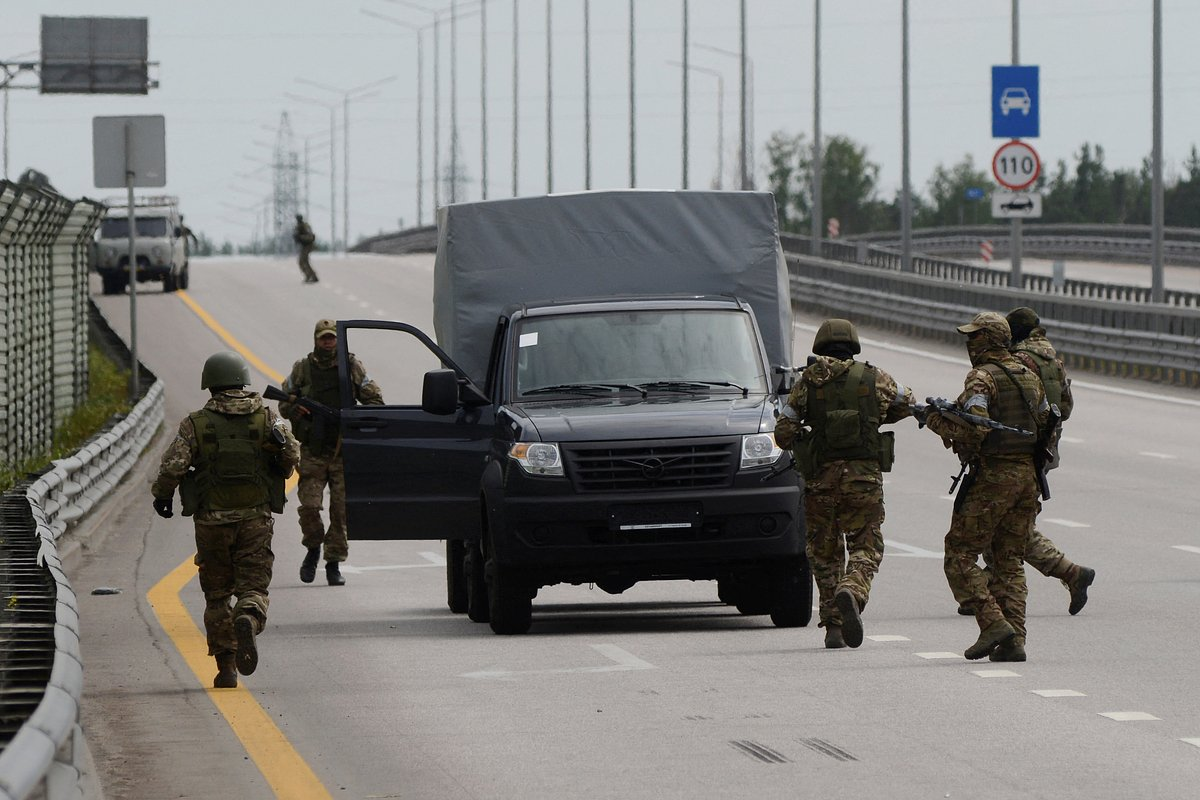
\includegraphics[width=0.75\textwidth]{img/pmc_africa_4.jpg}
    \caption{Бойцы ЧВК «Вагнер» обходят автомобиль на трассе М-4 недалеко от Воронежа, 24 июня 2023 года; Фото: Reuters}
\end{figure}

Что касается Мали, то Россия может быть заинтересована, например, в усилении роли Алжира в вопросах обеспечения безопасности в Сахаре, поскольку это североафриканское государство обладает значительным опытом в данной сфере и остается верным и крепким союзником России. Разумеется, сотрудничество с Алжиром никоим образом не должно идти в ущерб суверенитету Мали.

% -- <> -- 
\begin{fancyquotes}
    Поэтому российская сторона заинтересована в укреплении межгосударственных связей на региональном уровне и усилении африканского компонента в обеспечении безопасности. В долгосрочной перспективе это даст нам преимущества

    \begin{flushright}
        Андрей Маслов\\
        директор Центра изучения Африки НИУ ВШЭ
    \end{flushright}

\end{fancyquotes}

\textbf{Китайские стражи.} На африканском континенте, помимо ЧВК «Вагнер», работает множество частных военных компаний: американские CACI и Constellis, британские Aegis Defence Services и G4S, французская Secopex, немецкая Asgaard и многие другие.

\begin{center}
    \Large
    Специалисты затрудняются назвать даже примерное число иностранных наемников в Африке
\end{center}

Дело в том, что местные политические силы не любят афишировать свои связи с подобными структурами, а сами компании, как правило, заключают соглашения о неразглашении, запрещающие им делиться подробной информацией о характере их работы в африканских странах.

Впрочем, Андрей Маслов усомнился, что западные военные компании могут создать альтернативу ЧВК «Вагнер», поскольку изначально занимают другую нишу, работая с корпоративным сектором и занимаясь охраной объектов западных добывающих компаний. Африканские государства-заказчики же при выборе подрядчиков исходят из своих внешнеполитических приоритетов, а не из рыночных условий: что Мали, что ЦАР воспринимали ЧВК «Вагнер» как рекомендованную российским государством структуру.

\begin{fancyquotes}
    Какой частной она бы ни была, для Мали и ЦАР важно то, что она российская. Поэтому вряд ли произойдет вытеснение ЧВК «Вагнер» иностранными структурами на рыночных условиях


    \begin{flushright}
        Андрей Маслов\\
        директор Центра изучения Африки НИУ ВШЭ
    \end{flushright}

\end{fancyquotes}


\begin{figure}[h]
    \centering
    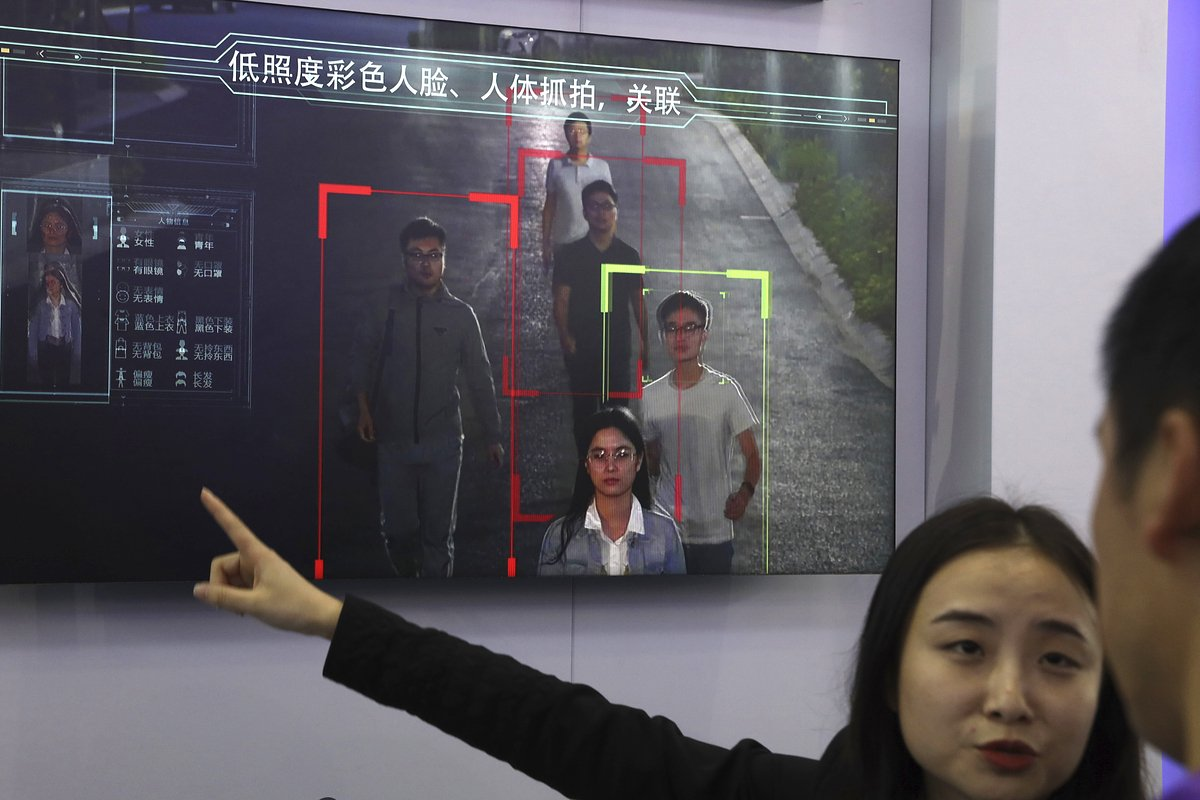
\includegraphics[width=0.75\textwidth]{img/pmc_africa_5.jpg}
    \caption{Презентация технологии идентификации человека от государственного производителя оборудования для наблюдения Hikvision на выставке Security China 2018 в Пекине, Китай, 23 октября 2018 года; Фото: Ng Han Guan / AP}
\end{figure}

Особняком стоят частные охранные фирмы из Китая, начавшего масштабную экономическую экспансию на континент в рамках запущенной в 2013 году инициативы «Один пояс — один путь»: соответствующие соглашения подписаны с 52 из 54 африканских стран. К настоящему моменту в Африке работает около 10 тысяч китайских компаний и, по разным оценкам, от 1 до 2 миллионов китайских рабочих, задействованных в развитии инфраструктуры, строительстве жилья, промышленном производстве и добыче полезных ископаемых.

Однако обстановка с безопасностью в ряде африканских стран оставляет желать лучшего: на континенте орудуют многочисленные вооруженные группировки, для которых похищение иностранных рабочих — один из основных источников дохода. Рабочих из Китая считают лакомой добычей: китайские корпорации, как правило, не жалеют денег, чтобы вызволить своих сотрудников.

\begin{center}
    \Large
    Полагаться на местные органы безопасности не приходится, тем более с учетом довольно неспокойной внутриполитической обстановки в ряде стран Африки: китайские рабочие не раз оказывались буквально меж двух огней враждующих фракций
\end{center}

Все это подтолкнуло китайскую сторону к тому, чтобы самостоятельно заняться защитой своих граждан, благо есть кем: в Поднебесной зарегистрировано свыше пяти тысяч частных охранных компаний, в которых работает около четырех миллионов человек, преимущественно из числа бывших военных.

\begin{center}
    \Large
    Частные военные компании в Китае запрещены, а все охранные предприятия строго подконтрольны Министерству общественной безопасности КНР
\end{center}

За пределами Китая разрешено работать всего 20 компаниям, а в Африке работает по меньшей мере девять из них: Beijing DeWe Security Service, Hua Xin Zhong An Group, Shandong Huawei Security Group, China Security Technology Group, China Overseas Security Group, Frontier Services Group, China Overseas Security Service, VSS Security Group и Zhongjun Junhong Security Service.


\begin{figure}[h]
    \centering
    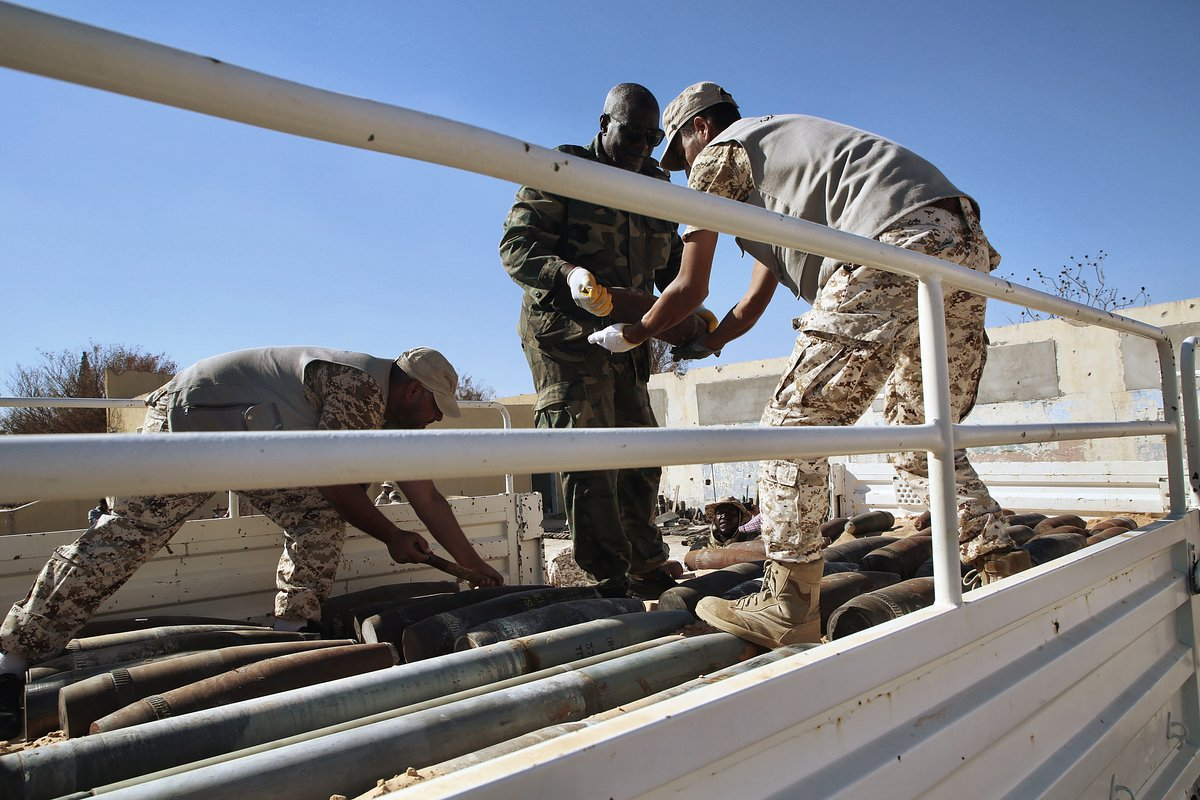
\includegraphics[width=0.75\textwidth]{img/pmc_africa_6.jpg}
    \caption{Ливийские ополченцы и специалсты из ЧВК «Вагнер» на погрузке боеприпасов, район Аль-Хира, в 75 километрах к югу от Триполи, Ливия, 22 июля 2020 года; Фото: Hazem Turkia / Anadolu Agency / Getty Images}
\end{figure}

По официальным данным, за границей работают всего 3200 сотрудников китайских частных охранных фирм, но исследователи полагают, что цифры сильно занижены: в одной лишь Кении защитой строительства железной дороги Момбаса — Найроби — Найваша занималось 2000 сотрудников DeWe.

Василий Кашин, директор Центра комплексных европейских и международных исследований НИУ ВШЭ и специалист по китайскому военно-промышленному комплексу, отмечает, что подавляющему большинству подобных фирм запрещено пользоваться оружием. Исключение составляют сотрудники Overseas Security Guardians и Hua Xin Zhong An Group, которые обеспечивают вооруженный конвой для китайских судов, следующих в африканских водах.

В остальных случаях сотрудники подобных фирм организуют охрану китайских предприятий с помощью нелетальных вооружений, решают технические задачи и выстраивают партнерство с местными охранными структурами. «А задачи, требующие использования оружия, они решают как раз за счет найма местных партнеров», — рассказал Василий Кашин в беседе с «Лентой.ру».

Например, в июле 2016 года DeWe прибегла к найму местных вооруженных сотрудников, чтобы эвакуировать свыше 300 китайских нефтяников из южно-суданской столицы Джубы, в которой разгорелось вооруженное противостояние между правительственными и оппозиционными силами.

Таким образом, китайские охранные предприятия значительно отличаются от структур ЧВК «Вагнер» — и по своему устройству, и по своим задачам, а потому вряд ли станут альтернативой российской компании в случае ее ухода с континента, считает специалист.

\begin{fancyquotes}
    Китайцам страшно помыслить о том, чтобы разрешить своему охранному бизнесу заниматься тем же, чем занимался «Вагнер»

    \begin{flushright}
        Василий Кашин\\
        директор Центра комплексных европейских и международных исследований НИУ ВШЭ
    \end{flushright}
\end{fancyquotes}

\textbf{Новые башибузуки.} Еще один игрок на африканском континенте, который может воспользоваться уходом вагнеровцев, — турецкая частная военная компания Sadat International Defense Consultancy, основанная в 2012 году. На официальном сайте утверждается, что SADAT — это «первая и единственная частная ЧВК в Турции, которая на международном уровне предоставляет услуги консалтинга, военной подготовки и логистики в секторе международной обороны и внутренней безопасности».

\begin{center}
    \Large
    Одним из главных преимуществ турецкой ЧВК SADAT считается наличие «готовых военно-воздушных сил», вооруженных беспилотниками Bayraktar, зарекомендовавшими себя в конфликтах на Украине, в Нагорном Карабахе и Ливии
\end{center}

\begin{figure}[h]
    \centering
    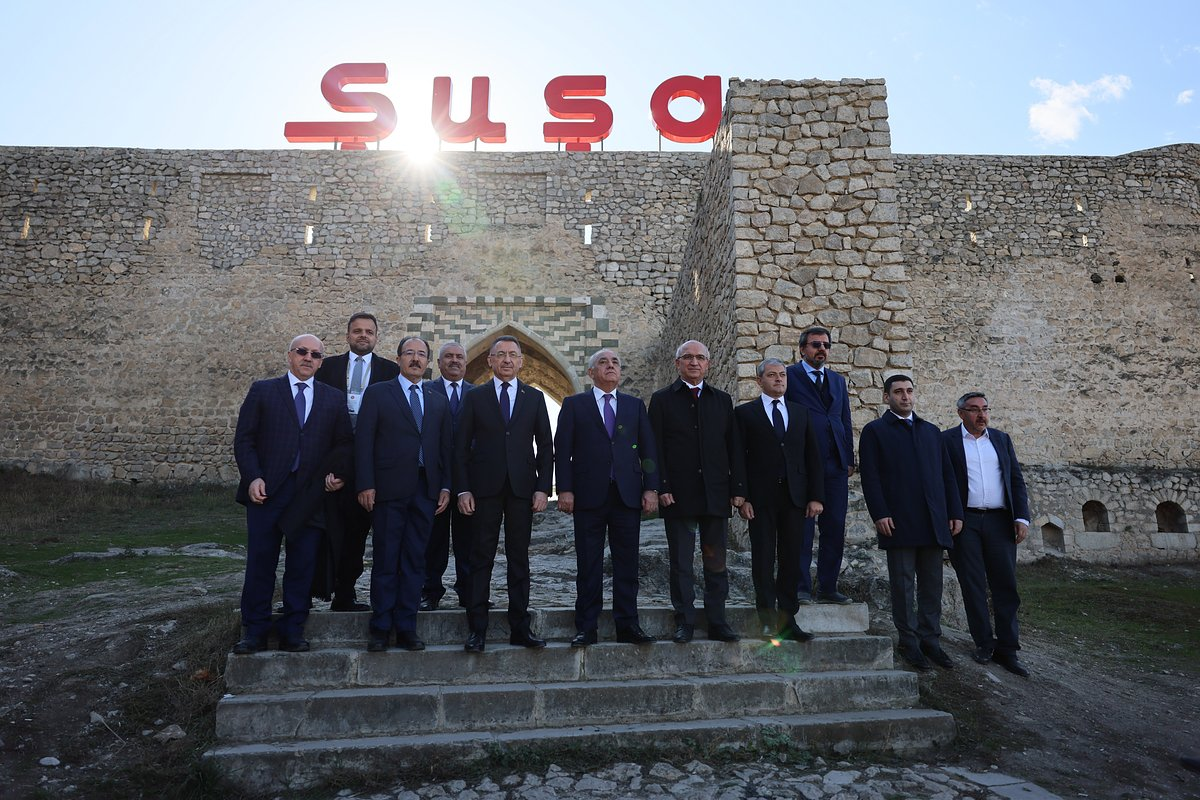
\includegraphics[width=0.75\textwidth]{img/pmc_africa_7.jpg}
    \caption{Вице-президент Турции Фуат Октай и премьер-министр Азербайджана Али Асадов посещают город Шуша в Нагорном Карабахе, Азербайджан, 5 ноября 2022 года; Фото: Berke Bayur / Anadolu Agency / Getty Images}
\end{figure}


Ряд наблюдателей считает SADAT личной армией президента Турции Реджепа Тайипа Эрдогана. Во время попытки госпереворота в июле 2016 года бойцы SADAT участвовали в подавлении протестов и, вероятно, даже стреляли по гражданским, рассказывает старший научный сотрудник American Enterprise Institute Майкл Рубин. С 2016 по 2022 год основатель SADAT Аднан Танрыверди также занимал пост главного военного советника турецкого лидера. При этом сам Реджеп Эрдоган опровергает всякие обвинения в покровительстве ЧВК.

По различным данным, SADAT работает в Сомали и Катаре, сотрудничала с палестинским движением ХАМАС и обучала ливийских повстанцев и сирийских боевиков, выступавших против правительства Башара Асада, в том числе якобы завербованных на Кавказе бойцов «Исламского государства» и «Джебхат ан-Нусры» (террористическая группировка, запрещенная в России).

ЧВК, вероятно, также была активно задействована и в конфликте в Нагорном Карабахе осенью 2020 года. По сведениям газеты «Коммерсант», SADAT занималась вербовкой и подготовкой сирийских боевиков на подконтрольных Турции территориях на севере и северо-западе Сирии, после чего обученных наемников — около 1,3 тысячи бойцов — перебросили в зону конфликта на чартерах, зафрахтованных все той же SADAT.

Кроме того, осенью 2022 года сообщалось о планах ЧВК направить своих наемников в Кашмир, являющийся предметом территориального спора между Индией и Пакистаном.

\begin{center}
    \Large
    В самом SADAT настаивают, что не участвуют в конфликтах в качестве наемников, а оказывают исключительно консультационные и образовательные услуги
\end{center}


\begin{figure}[h]
    \centering
    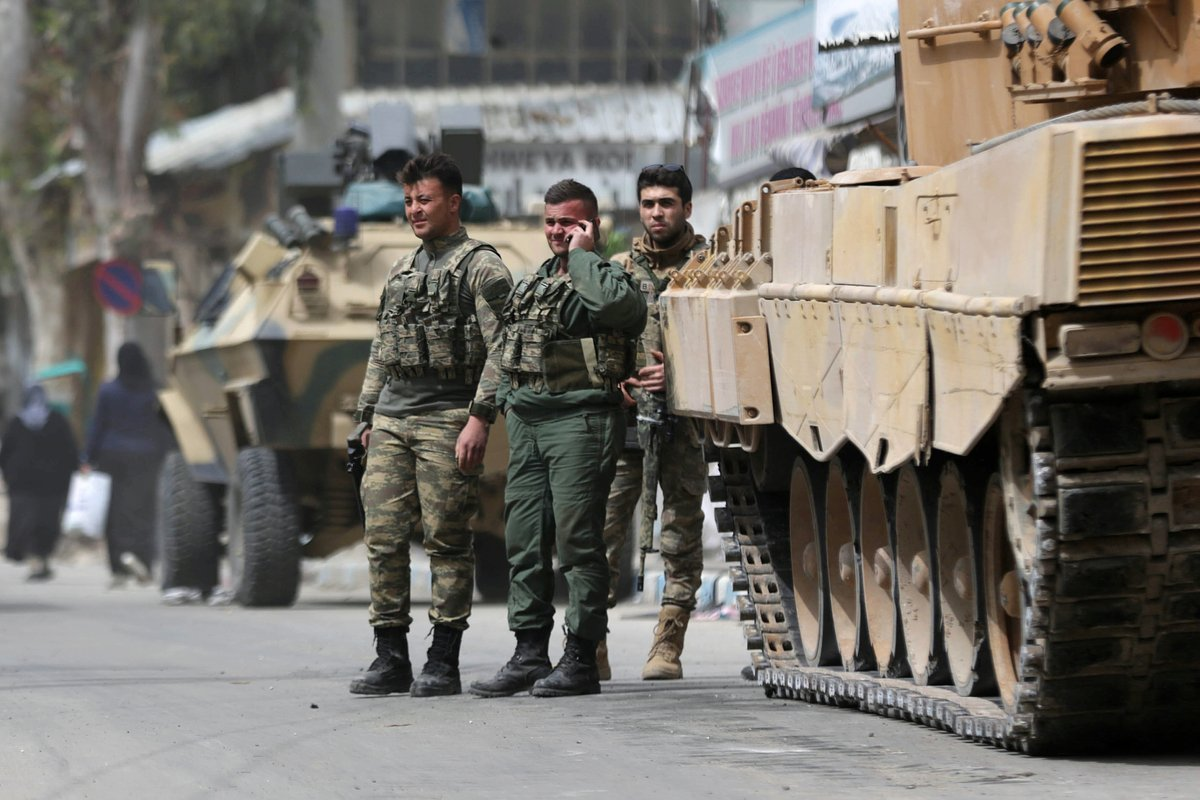
\includegraphics[width=0.75\textwidth]{img/pmc_africa_8.jpg}
    \caption{Турецкие солдаты в центре Африна, Сирия, 24 марта 2018 года; Фото: Khalil Ashawi / Reuters}
\end{figure}

Как и многие другие страны, в последние годы Турция активно развивает официальные связи с Африкой: страна значительно расширила свою сеть посольств на континенте, а ее президент посетил больше африканских государств, чем кто-либо из неафриканских лидеров.

Особое внимание уделяется наращиванию военно-технического сотрудничества с Африкой: лишь за 2021 год поставки турецкого военного оборудования на континент выросли в пять раз, правда, занимают пока меньше одного процента от рынка. Впрочем, этот показатель, вероятнее всего, продолжит расти — не в последнюю очередь благодаря растущей популярности турецких дронов Bayraktar.

Помимо Ливии, турецкие военные присутствуют в Сомали, где обучают местных солдат и офицеров военному ремеслу, причем на турецком языке, а сомалийские новобранцы даже приносят присягу сразу на двух языках. Кроме того, турецкие военнослужащие задействованы в миротворческих миссиях ООН в Демократической Республике Конго, Мали, Сомали, Судане, Южном Судане и ЦАР.

Впрочем, основатель SADAT Аднан Танрыверди еще в 2019 году призвал к переменам: по его словам, Турции необходимо создать полноценный аналог американской Blackwater, бойцы которой отправятся выполнять военные задачи в Африку, тогда как официальные вооруженные силы сосредоточатся на обороне собственной страны.

\begin{fancyquotes}
    Турция имеет глубоко укоренившиеся военные традиции. ЧВК могут оказывать услуги дружественным странам, нанимая отставных и недавно демобилизованных солдат. А затем их можно будет использовать как инструмент внешней политики

    \begin{flushright}
        Аднан Танриверди\\
        основатель SADAT
    \end{flushright}
\end{fancyquotes}

Впрочем, чтобы отказаться от услуг россиян в пользу турков, африканские государства, где сейчас работает ЧВК «Вагнер», должны будут сначала изменить свой политический курс, отмечает Андрей Маслов.

\begin{fancyquotes}
    Но пока предпосылок к тому, чтобы ЦАР или Мали поменяли свой внешнеполитический вектор, мы не видим

    \begin{flushright}
        Андрей Маслов\\
        директор Центра изучения Африки НИУ ВШЭ
    \end{flushright}
\end{fancyquotes}

Сам основатель SADAT Аднан Танрыверди другим важным условием считает разработку турецкими властями законодательства, которое бы устанавливало контроль государства над будущими военными компаниями. Мятеж Евгения Пригожина, вероятно, может ускорить этот процесс. Впрочем, все те же события 24 июня могут заставить Реджепа Эрдогана, наоборот, более настороженно отнестись к легализации и расширению сферы деятельности ЧВК — тем более что в 2016 году он уже пережил одну попытку госпереворота.

Китайские и турецкие ЧВК вряд ли сумеют составить достойную альтернативу ЧВК «Вагнер» в обозримом будущем: и в силу их текущей структуры и сфер деятельности, и в силу того, что сами Китай с Турцией, по всей видимости, не особо к этому стремятся. Западные ЧВК тоже не смогут претендовать на нишу вагнеровцев — их клиенты в основной своей массе крайне негативно относятся к перспективе сотрудничества с «неоколониальными силами» и изначально обратились к россиянам именно из этих соображений.

\begin{center}
    \Large
    Наконец, не похоже на то, что Россия сама готова отказаться от целого измерения сотрудничества со странами континента
\end{center}

Вероятно, российские власти выработают какое-то решение, которое позволит специалистам ЧВК «Вагнер» и дальше оказывать свои услуги в странах Африки в обмен на определенные гарантии лояльности. А уж под каким брендом — особой роли не играет: в африканских странах дали четко понять, что будут рады любым российским «музыкантам» — хоть «бетховенам», хоть «моцартам».

\newpage
\section{Караганов призвал Кремль нанести ядерный удар по Польше}

\textit{Спецкор «Медузы» Андрей Перцев объясняет, почему эти угрозы на самом деле опаснее, чем оголтелые посты Дмитрия Медведева}

\textit{Источник: \url{https://meduza.io}}
% https://meduza.io/feature/2023/06/15/politolog-sergey-karaganov-prizval-kreml-nanesti-yadernyy-udar-po-polshe

\textit{Журнал «Профиль» опубликовал — а издание «Россия в глобальной политике» перепечатало — статью политолога Сергея Караганова, суть которой сводится к тому, что Россия «должна нанести превентивный ядерный удар по Европе», чтобы «сломить волю Запада» и \explain{добиться победы}{achieve victory; добиться + чего} в войне с Украиной. Угрозы применения ядерного оружия со стороны Москвы звучат буквально с первых недель полномасштабной агрессии (этим занимается и сам Путин). Тем не менее статья Караганова, к сожалению, выглядит не просто очередным сотрясанием воздуха. \ed{Спецкор}{спецкор}{специальный корреспондент} «Медузы» Андрей Перцев объясняет почему.
}

\textbf{Кто такой Сергей Караганов? И почему его статья вообще \explain{заслуживает внимания}{deserved attention}?}

Доктора исторических наук и политолога Сергея Караганова вы, возможно, помните по проекту «\ed{Намедни}{нам\'{е}дни}{на днях; недавно}. Наша эра» журналиста Леонида Парфенова. Он комментировал советскую политическую историю — и делал это во вполне либеральном ключе. Еще в 2011 году Караганов, например, проповедовал «декоммунизацию» и «десталинизацию».

С тех пор многое поменялось. Сейчас Сергей Караганов --- один из основателей российского Совета по внешней и оборонной политике (СВОП). Это экспертный центр, с которым сотрудничают бывшие военные, дипломаты, действующие политики, исследователи и журналисты. В 2004 году СВОП стал одним из учредителей клуба «Валдай», в заседаниях которого регулярно участвует Путин. Сам Караганов, разумеется, тоже посещает эти встречи. Заседания клуба модерирует его соратник по СВОП, журналист-международник и политолог Федор Лукьянов. Он же возглавляет журнал «Россия в глобальной политике», а Караганов руководит редакционным советом издания.

\begin{wrapfigure}{l}{0.45\textwidth}
    \centering
    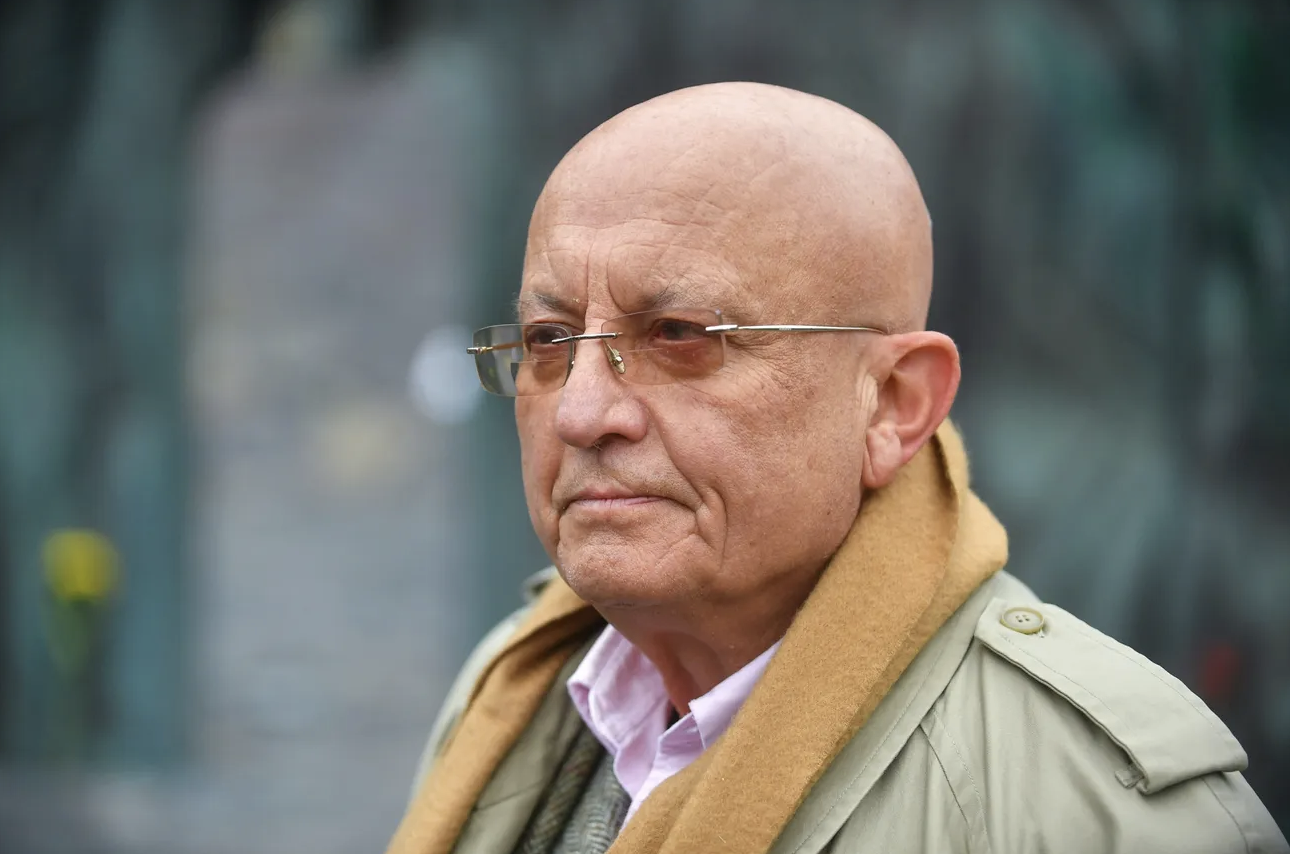
\includegraphics[width=0.43\textwidth]{img/karaganov.png}
    \caption{Сергей Киселев / Агентство «Москва»}
\end{wrapfigure}
У Караганова есть еще одна высокая регалия --- научный руководитель факультета мировой экономики и мировой политики Высшей школы экономики. Но самое главное, что он входит в состав научного совета при Совете безопасности РФ, который на фоне вторжения стал, по всей видимости, ключевым органом власти в России. Два источника «Медузы», близких к администрации президента (АП), называют Караганова человеком, который «может влиять на мнение секретаря Совбеза Николая Патрушева». А тот, в свою очередь, как считается, входит в близкий круг Путина.

Впрочем, третий собеседник «Медузы», близкий к Кремлю, призывает «не преувеличивать влияние Караганова». Тем не менее политолог реально участвует в деятельности Совета безопасности РФ и регулярно бывает на мероприятиях с участием Путина.

По косвенным признакам можно предположить, что руководители силового блока как минимум знакомы с идеями Караганова, а может быть, даже \explain{вдохновляются}{are inspired} ими. Вы наверняка слышали эксцентричные высказывания Николая Патрушева и главы Службы внешней разведки Сергея Нарышкина о том, что Польша «готовится захватить украинские земли» (подробнее об этом читайте, например, \href{https://carnegieendowment.org/politika/88530}{тут}). Так вот: Караганов \href{https://globalaffairs.ru/articles/rakety-v-evrope-vospominaniya-o-budushhem/}{рассуждал} об этом еще в 2016 году:

\begin{fancyquotes}
    Она (Украина) вряд ли может состояться как государство в долгосрочной перспективе. Скорее всего, страна будет медленно распадаться. Ну а там история покажет. Не исключено, что что-то может отойти к России, что-то — к Венгрии, что-то — к Польше, а что-то может остаться формально независимым Украинским государством.
\end{fancyquotes}

\textbf{Дмитрий Киселев в прямом эфире грозил превратить США в «радиоактивный пепел» еще до аннексии Крыма. А недавно ядерным ударом пугал Запад Дмитрий Медведев. Неужели слова политолога Караганова значат больше?}

В каком-то смысле да. Дмитрий Киселев в середине 2010-х был главным пропагандистом российской власти. В этом качестве он театрально и, \explain{по всей видимости}{apparently}, совершенно \explain{осознанно}{consciously} \explain{эпатировал}{shocked, scandalised} либерально настроенных \ed{сограждан}{согражданин}{fellow citizen} --- выступая с речами, вызывающими ужас и стыд, но не имеющими никаких последствий. Примерно тем же (несмотря на свой прежний и нынешний\footnote{Формально бывший президент и бывший премьер Медведев остается заместителем Путина в Совбезе РФ. Эту должность придумали специально для него, чем он там занимается, неизвестно.} высокий статус) занимается и Медведев, который в своем телеграм-канале оскорбляет западных политиков и жителей других стран.

В случае Киселева и Медведева угрозы ядерным оружием воспринимаются в ряду других не менее жестких заявлений. В отличие от Киселева и Медведева, Караганов всегда вел себя сдержанно. При этом его статья перепечатана в журнале «Россия в глобальной политике»: это медиа когда-то было запущено по модели западного аналитического издания при участии американского журнала Foreign Affairs — и до последнего времени считалось серьезным и уважаемым. Даже после 24 февраля журнал не исключили из международных баз данных научных публикаций (например, Scopus), то есть публиковаться там, в том числе зарубежным ученым, по-прежнему допустимо и даже — теоретически — престижно.

Статью Караганова, вероятно, можно воспринять как личную инициативу, попытку послать сигнал высшему руководству страны — и предложить свой радикальный вариант выхода из кризиса, в котором Россия оказалась из-за военной агрессии против Украины. С другой стороны, учитывая близость Караганова к Совбезу РФ и его личное участие в организации «Валдая», этот текст вполне может транслировать мнение, распространенное в силовом — самом влиятельном — блоке российской власти.

\textbf{То есть это статья написана лично для Путина?}

Возможно. \ed{В пользу}{в пользу}{in favour} этой версии говорит риторика, которую использует Сергей Караганов. Она очень близка российскому президенту: политолог явно пытается соответствовать путинскому языку. Например, в тексте встречается «пацанская аргументация», характерная для президента РФ: в частности, когда Караганов объясняет, что превентивный ядерный удар по Европе нужен, «чтобы Запад просто ``отвалил'' и не мешал\footnote{мешать + кому} России и миру идти вперед». Не забыл Караганов упомянуть и «неоколониализм», который в последние полтора года \explain{к месту}{in place} и не к месту вспоминает Путин.

Или вот еще одно, по сути, повторение излюбленных путинских клише:

\begin{fancyquotes}
    Запад теряет имевшуюся у него на протяжении пяти веков возможность \ex{высасывать}{suck} богатство из всего мира, \ed{навязывая}{навязывать}{to impose}, в первую очередь грубой силой, политические, экономические порядки и устанавливая свое культурное доминирование. Так что быстрого окончания развертываемой Западом оборонительной, но агрессивной конфронтации ожидать не приходится.
\end{fancyquotes}

Караганов вспоминает также «отрицание семьи, родины, истории, любви между мужчиной и женщиной, веры, служения высшим идеалам, всего того, что составляет сущность человека» --- все это, разумеется, на Западе. Узнаете? Да, Путин тоже об этом много и часто говорит.

При этом автор успокаивает своего потенциального высокопоставленного читателя --- того самого, который гипотетически может принять решение о применении ядерного оружия: США якобы не \ed{вст\'{у}пятся за}{вступ\'{и}ться за кого-либо}{to stand up for} Европу, никто не будет жертвовать «условным Бостоном ради условной Познани». Караганов \ex{подкрепляет}{reinforces} эту мысль еще одним опасным тезисом: «Победителей не судят, а спасителей благодарят». А что победа в итоге окажется за Россией, как бы само собой разумеется.

Насколько лет назад Караганов доказывал, что ядерное оружие, которым располагает Россия, было залогом отказа Запада от поставок оружия Украине во время войны в Донбассе 2014–2015 годов:

\begin{fancyquotes}
    Когда горячие головы в Вашингтоне требовали поставки Киеву «летальных вооружений», европейцы, да и руководство США категорически это \ex{отвергли}{rejected}, поскольку понимали, что Россия, прикрытая ядерным оружием и обретшая волю к борьбе, ответит крайне жестко.
\end{fancyquotes}

Но теперь, когда США и страны Евросоюза такое вооружение поставляют, получается, что Россия просто «обязана» сделать следующий опаснейший шаг.

Если Караганов (один или вместе с влиятельными единомышленниками) действительно хочет убедить президента РФ в необходимости нанести ядерный удар, вполне логично, что он доносит эту мысль в приятной и знакомой Путину обертке.

\textbf{Довольно пугающая версия. А другие есть?}

Да. Возможно, Караганов пытается не убедить Путина ударить по Европе, а напугать влиятельных и высокопоставленных людей на Западе самой этой возможностью --- и склонить их к изменению позиции по Украине.

Здесь нужно еще раз вспомнить об эволюции взглядов политолога. Даже после аннексии Крыма их еще можно было назвать относительно миролюбивыми. В 2016 году Караганов предлагал российским властям такую программу:

\begin{fancyquotes}
    Лучше бороться за мир, \ex{выступать поставщиком безопасности}{act as a security provider}, в том числе предотвращая дальнейшую экспансию западных союзов, что мы, хотя и \ex{с запозданием}{belatedly}, сделали в 2014 г. [аннексировав Крым], срывать планы тех, кто хочет вернуть гонку вооружений и системный военно-политический конфликт, восстановить лидерство в борьбе за верховенство международного права, за стратегическую стабильность.
\end{fancyquotes}

Тогда политолог был уверен, что «планов по завоеванию Украины у нас точно нет». Однако уже в 2017 году Караганов начал фокусировать внимание на том, что «одной из основ формирования нового миропорядка» может стать диалог США, России и Китая по вопросу о ядерном сдерживании. Иными словами, он стремительно разуверился в идее борьбы за мир и «верховенстве международного права» и пришел к выводу, что ядерное оружие — более надежный гарант мира на планете, чем договоренности и принципы:

\begin{fancyquotes}
    «Большая тройка» будет закладывать основы для менее хаотичной и более безопасной мировой системы будущего. Этот новый «концерт наций», если и когда у лидеров трех стран хватит чувства ответственности создать его, может оказаться более устойчивым, чем предыдущий из XIX века, если он по согласию будет базироваться на взаимном ядерном сдерживании, а не только на моральных принципах или балансе сил.
\end{fancyquotes}

То есть уже как минимум шесть лет Караганов уверен, что только страх перед использованием ядерного оружия может удержать человечество от кровопролитной глобальной войны, — и пытается убедить в этом своих читателей.

Нынешняя статья продолжает эволюцию взглядов политолога. Если в 2017 году Караганов еще предлагал сторонам спокойно подумать о переговорах, то теперь он пытается посеять у читателей на Западе страх и заставить их согласиться на уступки.

Караганов, очевидно, надеется, что в западных странах заметят: теперь им угрожает не потерявший влияние бывший президент (выбравший в качестве публичной стратегии оскорбления в адрес всего, чем раньше сам восхищался) и не штатный пропагандист в популярном вечернем шоу (которому полагается выступать с самыми радикальными идеями). К ним со страниц авторитетного — как, очевидно, полагают в редакции — журнала обращается серьезный эксперт, который не так уж давно считал ядерный конфликт маловероятным.

Вероятно, с точки зрения Караганова, это должно послужить лишним аргументом, чтобы Запад наконец отказался от поддержки Украины. В статье такой вариант прямо проговаривается: «Все-таки велика вероятность, что удастся победить, образумить противника без крайних мер, заставить его отступить».

Иными словами, сам Караганов может считать свой текст дополнительным элементом «ядерного сдерживания».

\textbf{Но если статья Караганова — не более чем его личное послание (хоть Путину, хоть Западу), то бояться все равно нечего?}

К сожалению, даже в этом случае появление такой статьи — плохая новость. Во-первых, не будем забывать, что у автора могут быть влиятельные единомышленники. Во-вторых, слишком логичными и убедительными могут казаться Путину и его окружению рассуждения Караганова о ходе исторического процесса: Запад «умирает и теряет влияние»; его нужно огорошить мощным ударом; история будет «на нашей стороне».

Даже если цель Караганова только в том, чтобы напугать Запад, его статья вполне способна повлиять на решения руководства России. Из-за стремления звучать в унисон с Путиным текст может оказаться не элементом ядерного сдерживания, как, возможно, надеялся сам автор, а ступенькой вверх по лестнице ядерной эскалации.

Правда, аналитик британского исследовательского центра Chatham Housе Кеир Джайлс предлагает относиться к ядерным угрозам, звучащим из России, исключительно как к методу психологической войны. Как отмечает Джайлс, Кремль прибегает к этому методу всякий раз, когда у российской армии возникают реальные проблемы на фронте (а статья Караганова появилась вскоре после начала украинского контрнаступления). Но и Джайлс признает: Путин действительно ориентируется на пропагандистские СМИ и лояльных экспертов, и это может роковым образом влиять на решения президента РФ.

Вот понятный пример. Перед полномасштабным вторжением в Украину верхушка ФСБ убеждала Путина, что украинцы с цветами встретят российских солдат. Причем не факт, что все «ястребы» сами хотели большой войны — скорее, стремились угодить главе государства. Но в итоге, оперевшись на эти высказывания и оценки, Путин начал реальную агрессию.

Теперь игра, затеянная Карагановым с не самыми ясными намерениями, вполне может показаться руководству России планом легкой победы.
\chapter{Личность, Характер и Психология}
\section{Что такое думскроллинг}

\textit{и почему чтение плохих новостей пагубно влияет на ментальное здоровье?}

\textit{Источник: \url{https://www.elle.ru}}
% https://www.elle.ru/otnosheniya/psikho/chto-takoe-dumskrolling-i-pochemu-chtenie-plokhikh-novostei-pagubno-vliyaet-na-mentalnoe-zdorove/

\begin{fancyquotes}
    Постоянно просматриваете новости? Не выпускаете смартфон из рук? У нас для вас плохие новости  ---  вы зависимы, и это пагубно влияет на ваше здоровье и умственные способности.
\end{fancyquotes}

Думскроллинг (от английского doom  ---  «гибель, судьба, рок, Судный день» и scrolling  ---  «прокрутка»)  ---  это склонность к просмотру и чтению плохих новостей, несмотря на то, что они вызывают негативные эмоции, удручают, огорчают и деморализуют. Термин стал относительно широко использоваться в начале пандемии и сейчас снова стал актуален на фоне нестабильной ситуации в мире. Так почему же мы не можем оторваться от плохих новостей и как это влияет на наше психоэмоциональное состояние?

Основная причина бесконтрольного думскроллинга  ---  это боязнь пропустить важные новости. Беспокойный ум стремится понять, что происходит в мире и как это может коснуться лично нас. В таком случае думскроллинг дает ощущение контроля над ситуацией. Интуитивно мы пытаемся подготовиться к потенциальным угрозам. Принцип «предупрежден  ---  значит вооружён» миллионы лет способствует выживанию людей как вида.

\textbf{Почему это вредно?}

Иллюзия контроля над ситуацией, по большому счету, не дает никаких преимуществ. Думскроллинг способствует развитию тревожности и стресса, повышается вероятность панических атак, снижается концентрация. Умные алгоритмы соцсетей предлагают все больше и больше плохих новостей, поиск и чтение пугающих статей превращается в зависимость, человек игнорирует собственные мысли и чувства. Впоследствии чтение негативных новостей может приводить и к ухудшению сна и истощению нервной системы.

\textbf{Как бороться с думскроллингом?}

Не пользуйтесь гаджетами перед сном. Не читайте новостей о коронавирусе, войнах, протестах и других тревожных явлениях на ночь. Если вам сложно контролировать это самостоятельно, то установите будильник и за 2-3 часа до сна переводите телефон в авиарежим.

Читайте только ту информацию, которая вам нужна, не переключайте внимание на другие новости. Перед тем, как читать новости и статьи в интернете, четко определите «цель визита», не обращайте внимание на предложенные статьи или кликбейтные заголовки.

Отвлекитесь от новостного контента. Попробуйте сместить фокус внимания с новостей на интересные статьи, интервью, рецензии.

Займитесь чем-то другим. Кино, музыка, встречи с друзьями  ---  все это поможет провести вам время с куда большей пользой для нервной системы.

\newpage
\section{Синдром спасителя}

\textit{Как добрые намерения скрывают эмоциональные недостатки}

\textit{Что скрывает навязчивое желание помочь ближнему, если вас об этом никто не просит}

\textit{Источник: \url{https://www.elle.ru}}
% https://www.elle.ru/otnosheniya/psikho/sindrom-spasitelya-kak-dobrye-namereniya-skryvayut-emocionalnye-nedostatki/

Проявления синдрома спасителя не всегда очевидны для окружающих и даже тех, кого непрошеные благодетели окружают заботой. Импровизированные супергерои всегда готовы помочь нерасторопным коллегам, спасти близких (и не очень) людей от жизненных невзгод и пагубных пристрастий. Именно такие светлые человечки рады круглосуточно наставлять подшефных по вопросам правильного питания, карьерного роста и токсичных отношений. Ведомые убеждением, что в этом их высшее предназначение, «спасители» возводят альтруизм в культ, в действительности скрывая за самоотдачей эгоизм и невротические изъяны.

Термин «спаситель» используется психологами с 1968 года, с тех пор, как доктор Стивен Карпман, ученик Эрика Берна и знаток транзактного анализа, раскрыл в опубликованной работе модель социального и психологического взаимодействия, названную в его честь «треугольник Карпмана» (он же  ---  «треугольник судьбы» или Karpman drama triangle). В статье Fairy Tales and Script Drama Analysis американский ученый описал три привычные роли, которые мы часто играем в разных ситуациях: жертва, преследователь и спаситель, который вмешивается, как кажется, из желания помочь тому, кого обижают или недооценивают.

Как разъяснил Карпман, ролевая игра, схожая с мелодраматическим сюжетом про «героя, злодея и девицу в беде», раскрывает неочевидный мотив: спаситель заинтересован поддерживать жертву в ее зависимости от себя. Догадываетесь почему?

\textbf{Как из заботы получается созависимость}

«Нужда помогать другим движет личностью, способной реализоваться исключительно в опеке других,  ---  объясняет Анн-Виктуар Русселе, парижский психолог и терапевт.  ---  Такие люди считают своим долгом спасать других в ущерб себе, включая тех, кто в этом абсолютно не нуждается. Они сознательно вступают в созависимые отношения, считая, что не заслуживают любви партнера, но убеждая себя, что эта связь оправдана желанием избавить ее/его от проблем. Настойчивая услужливость имеет в корне нарциссический изъян, скрывающий неуверенность в себе и сопутствующую мотивацию: потребность поднять самооценку. „Спаситель“ становится лучше в собственных глазах, проецируя на ближних позитивные намерения и поступки».

Чего же следует ожидать от непрошеной заботы? «Спасаемые» увиливают от спасения, не предлагая взамен долгожданной компенсации, что, естественно, отзывается в душе супергероя горьким разочарованием. «Я делаю все для всех, но никто никогда ничего не делает для меня»,  ---  типичная жалоба отвергнутого спасителя.

«Последствия амбивалентного синдрома непременно дадут о себе знать,  ---  пишут калифорнийские психологи Мэри Ламиа и Мэрилин Кригер в книге „Синдром Белого Рыцаря: спасение себя от потребности спасти других“ (The White Knight Syndrome: Rescuing Yourself from Your Need to Rescue Other).  ---  В начале отношений спаситель кажется удовлетворенным своей самоотверженностью, но со временем становится все более несчастным и бессильным. Она/он буквально выдыхается, теряя смысл, интерес, энергию, ресурсы, что, в свою очередь, отражается на самооценке. Убедившись, что усилия напрасны, «белый рыцарь» выходит из игры эмоционально и психологически истощенным».

\textbf{В чем (опять) виноваты детские травмы}

Потребность спасать указывает на эмоциональный и психологический дисбаланс, ноги которого предсказуемо растут из воспитания, образования и внушенных ценностей. «Она/он спасает всех вокруг, стараясь быть „хорошей девочкой/мальчиком“, чтобы получить одобрение со стороны реального или внутреннего родителя и укрепить самооценку,  ---  описывает природу травмы доктор Русселе.  ---  Возможно, в детстве „спасителю“ приходилось помогать больной матери, заботиться о братьях и сестрах, с раннего возраста посвящая себя нуждам взрослых и опуская свои потребности в нижний ранг приоритетов».

Пресловутый дисбаланс имеет тенденцию преследовать «спасителя» до зрелости, поддерживая в ней/нем потребность окружить себя партнерами, друзьями и коллегами, о которых нужно будет заботиться. И эта иллюзорная стратегия предсказуемо обречена на неудачу, потому что суть всего успешного базируется на гармонии.

\textbf{Как избавиться от синдрома спасителя}

От самоотверженного поведения никто не застрахован, но, к счастью, существуют когнитивные методики, которые помогут скорректировать психологический разлад. «Чтобы избавиться от непреходящего стремления быть кому-то нянькой, бросьте все силы на прокачку самоуважения и любви к себе,  ---  призывают Мэри Ламиа и Мэрилин Кригер.  ---  «Спасителям» надо усилием воли сменить тактику, признав наконец, что их любят не за сервис, который они обеспечивают, а за то, кто они на самом деле».

Увязшим в «спасающем» паттерне непросто пойти на поправку  ---  изменить отношение к себе и окружающему миру мешает страх перед возможным одиночеством. А что, если опекаемые отвернутся и забудут насовсем? А что, если вместе с заботами о других из жизни исчезнет смысл?

Чтобы заблокировать страхи, доктор Русселе советует свести помощь к «контрактному» формату, а попросту  ---  договориться. «Если хотите подстраховать себя от разочарований, вместо того чтобы помогать без спроса, обсудите напрямую, чем вы можете быть полезны для конкретного человека. Так вы заранее поймете, готовы ли оказывать услуги без ожиданий безграничной признательности и вдобавок проявите реальную заботу о себе  ---  в кои-то веки. К тому же это хорошая практика в соблюдении личных границ, на которые каждый из нас имеет право».

\newpage
\section{Мой характер}
\textit{Источник: \url{https://ru4.ilovetranslation.com/yuYUND7JV3L=d/}}

О себе говорить приятно, но немного трудно. Приятно, потому что всем нравится говорить о своих интересах, вкусах и предпочтениях. Но это в то же время трудно, так как изучить человека, особенно себя самого, не так уж просто.

Прежде чем говорить о своем характере, хотелось бы сначала уточнить, что такое характер. Человек отличается от остальных своими качествами. Часто люди говорят, что я не такой как остальные. Но я не считаю, что я какой-то особенный. В темноте все кошки серые. Но если вы подойдете ближе и включите свет, вы увидите, что мне присущи определенные черты.

Но не будем вдаваться в подробности, и немного сократим рассказ. У меня хорошее чувство юмора, я ответственный, трудолюбивый и эмоциональный человек. Мне нравится творчество, и я ценю эту черту в других людях. Я не люблю ложь и чувствую, когда другие лгут.

Я стараюсь никогда не опаздывать и \explain{терпеть}{to brook} не могу, когда другие не приходят \explain{вовремя}{on time}. Я предпочитаю общаться с умными и вежливыми людьми. \explain{Досадно}{it's annoying}, когда тот, кому ты \explain{доверяешь}{доверять/доверить: to trust}, оказывается \explain{ненадежным}{ненадежный: unreliable} человеком.

Я стараюсь \explain{обращаться}{to treat / обратиться} с другими так, как я хотел бы, чтобы они обращались со мной. Я ищу человека со здоровым и сильным ум\'{о}м и телом. Человека, с которым интересно общаться, которому я могу доверять и на кого можно положиться.

Что касается моих интересов, мне нравится психология в плане общения с людьми, а также способа формирования мыслей наилучшим образом. Я очень люблю путешествовать, встречаться с новыми людьми, знакомиться с их традициями и обычаями, их культурой, смотреть достопримечательности. Мне также нравятся разные стили музыки, нравится ритмичная музыка, под которую можно танцевать.

\newpage
\section{Психоанализ Зигмунда Фрейда}

\textit{Предпосылки и базовые идеи за 5 минут}

\textit{Источник: \url{https://bit.ly/3sfBWgd}}

Изучением психики человека уже не один десяток лет занимаются великие умы, но на многие вопросы ответов до сих пор нет. Что скрывается в глубинах человеческого существа? Почему события, произошедшие когда-то в детстве, по сей день оказывают влияние на людей? Что заставляет нас совершать одни и те же ошибки и мёртвой хваткой держаться за опостылевшие отношения? Где берут своё начало сновидения, и какая информация в них заложена? На эти и множество других вопросов, относительно психической реальности человека, может ответить революционный и поправший собой многие основы психологии психоанализ, созданный выдающимся австрийским учёным, неврологом и психиатром Зигмундом Фрейдом.

\textbf{Как появился психоанализ?}

В самом начале своей деятельности Зигмунд Фрейд успел поработать с выдающимися учёными своего времени – физиологом Эрнстом Брюкке, практикующим гипноз врачом Иосифом Брейером, неврологом Жаном-Маре Шарко и другими. Часть мыслей и идей, которые зародились на этом этапе, Фрейд развивал и в своих дальнейших научных трудах.

Если говорить более конкретно, то ещё молодого тогда Фрейда привлекло то, что некоторые симптомы истерии, проявлявшиеся у больных ею, не могли никак быть интерпретированы с физиологической точки зрения. К примеру, человек мог ничего не чувствовать в одной области тела, несмотря на то, что в соседних областях чувствительность сохранялась. Ещё одним доказательством того, что далеко не все психические процессы могут быть объяснены реакцией человеческой нервной системы или актом его сознания, было наблюдение за поведением людей, которые подвергались гипнозу.

Сегодня все понимают, что если находящемуся под гипнозом человеку внушить приказ что-либо выполнить, после своего пробуждения он бессознательно будет стремиться к его выполнению. А если поинтересоваться у него, почему он хочет это сделать, он сможет привести вполне адекватные объяснения своему поведению. Отсюда и получается, что психика человека имеет свойство самостоятельно создавать объяснения каким-то поступкам, даже если в них нет никакой необходимости.

В современность Зигмунда Фрейда само понимание того, что действиями людей могут управлять скрытые от их сознания причины, стало шокирующим откровением. До исследований Фрейда таких терминов как «подсознательное» или «бессознательное» не было вовсе. И его наблюдения стали отправной точкой в развитии психоанализа – анализа человеческой психики с позиции движущих ею сил, а также причин, последствий и воздействия на последующую жизнь человека и состояние его нервно-психического здоровья опыта, полученного им в прошлом.

\textbf{Базовые идеи психоанализа}

Теория психоанализа зиждется на том утверждении Фрейда, что в психической (если удобнее – душевной) природе человека не может быть непоследовательности и перерывов. Любая мысль, любое желание и любой поступок всегда имеет свою причину, обусловленную сознательным или бессознательным намерением. События, имевшие место в прошлом, влияют на будущие. И даже если человек убеждён, что какие-либо его душевные переживания не имеют оснований, всегда присутствуют скрытые связи между одними событиями и другими.

Исходя из этого, Фрейд разделял психику человека на три отдельные области: область сознания, область предсознания и область бессознательного.

\begin{enumerate}
    \item К области бессознательного относятся бессознательные инстинкты, никогда не доступные сознанию. Сюда же можно отнести вытесненные из сознания мысли, чувства и переживания, которые воспринимаются сознанием человека как не имеющие права на существование, грязные или запрещённые. Область бессознательного не подчиняется временным рамкам. Например, какие-то воспоминания из детства, вдруг снова попав в сознание, будут такими же интенсивными, как и в момент своего появления.
    \item К области предсознания относится часть области бессознательного, способная в любой момент стать доступной для сознания.
    \item Область сознания включает в себя всё то, что осознаёт человек в каждый момент своей жизни.
\end{enumerate}

Основными действующими силами человеческой психики, согласно идеям Фрейда, являются именно инстинкты – напряжения, которые направляют человека к какой-либо цели. И эти инстинкты включают в себя два главенствующих:

\begin{enumerate}
    \item Либидо, являющееся энергией жизни
    \item Агрессивная энергия, являющаяся инстинктом смерти
\end{enumerate}

Психоанализ рассматривает, по большей части, либидо, в основе которого лежит сексуальная природа. Оно представляет собой живую энергию, характеристики которой (появление, количество, перемещение, распределение) могут истолковать любые психические расстройства и особенности поведения, мыслей и переживаний индивида.

Личность человека, согласно психоаналитической теории, представлена тремя структурами:
\begin{enumerate}
    \item Оно (Ид)
    \item Я (Эго)
    \item Сверх-Я (Супер-Эго)
\end{enumerate}

Оно (Ид) является всем изначально заложенным в человеке – наследственностью, инстинктами. На Ид никак не влияют законы логики. Его характеристики  ---  это хаотичность и неорганизованность. Но Ид воздействует на Я и Сверх-Я. Причём, его воздействие безгранично.

Я (Эго) является той частью личности человека, которая находится в тесном контакте с окружающими его людьми. Эго берёт своё начало из Ид с того самого момента, когда ребёнок начинает осознавать себя как личность. Ид питает Эго, а Эго защищает его, словно оболочка. То, как взаимосвязаны Эго и Ид, легко отобразить на примере потребности в сексе: Ид могло бы осуществить удовлетворение этой потребности посредством прямого сексуального контакта, но Эго решает, когда, где и при каких условиях этот контакт может быть реализован. Эго способно перенаправлять или сдерживать Ид, тем самым являясь гарантом обеспечения физического и душевного здоровья человека, а также его безопасности.

Сверх-Я (Супер-Эго) произрастает из Эго, являясь хранилищем моральных устоев и законов, ограничений и запретов, которые накладываются на личность. Фрейд утверждал, что Сверх-Я выполняет три функции, коими являются:
\begin{enumerate}
    \item Функция совести
    \item Функция самонаблюдения
    \item Функция, формирующая идеалы
\end{enumerate}

Оно, Я и Сверх-Я необходимы для совместного достижения одной цели – поддержания равновесия между стремлением, ведущим к увеличению удовольствия, и опасностью, возникающей от неудовольствия.

Возникшая в Оно энергия отражается в Я, а Сверх-Я определяет границы Я. Учитывая то, что требования Оно, Сверх-Я и внешней реальности, к которой должен приспособиться человек, нередко являются противоречивыми, это неизбежно приводит к внутриличностным конфликтам. Решение же конфликтов внутри личности происходит посредством нескольких способов:
\begin{enumerate}
    \item Сновидения
    \item Сублимация
    \item Компенсация
    \item Блокировка механизмами защиты
\end{enumerate}

Сновидения могут быть отражением желаний, не реализованных в реальной жизни. Сновидения, которые повторяются, могут быть указателями на определённую потребность, которая не была реализована, и которая может служить помехой на пути свободного самовыражения человека и его психологического роста.

Сублимация является перенаправлением энергии либидо на цели, одобряемые обществом. Нередко такими целями выступает творческая, социальная или интеллектуальная деятельность. Сублимация есть форма успешной защиты, а сублимированная энергия создаёт то, что все мы привыкли называть словом «цивилизация».

Состояние тревожности, которое возникает от неудовлетворённого желания, есть возможность нейтрализовать через прямое обращение к проблеме. Так, энергия, которая не может найти выхода, будет направлена на преодоление препятствий, на уменьшение последствий этих препятствий и на компенсацию того, чего не хватает. В качестве примера можно привести идеальный слух, который развивается у слепых или слабовидящих людей. Человеческая психика способна поступить аналогичным образом: к примеру, у человека, страдающего недостатком способностей, но имеющего сильнейшее желание достичь успеха, может развиться непревзойдённая работоспособность или беспримерная напористость.

Однако бывают и такие ситуации, в которых появившееся напряжение может быть искажено или отвергнуто особыми защитными механизмами, такими как гиперкомпенсация, регрессия, проекция, изоляция, рационализация, отрицание, подавление и другими. Например, неразделённую или потерянную любовь можно подавить («Не помню никакой любви»), отвергнуть («Да любви и не было»), рационализировать («Те отношения были ошибкой»), изолировать («Мне не нужна любовь»), спроецировать, приписав другим свои чувства («Люди не умеют любить по-настоящему»), гиперкомпенсировать («Я предпочитаю свободные отношения») и т.д.

\textbf{Краткое резюме}

Психоанализ Зигмунда Фрейда – это величайшая попытка прийти к пониманию и описанию тех составляющих психической жизни человека, которые до Фрейда были непостижимыми. Самим же термином «психоанализ» в настоящее время называют:

\begin{enumerate}
    \item Научную дисциплину
    \item Комплекс мероприятий по исследованию психических процессов
    \item Методику лечения нарушений невротического характера
\end{enumerate}


Работа Фрейда и его психоанализ даже сегодня нередко критикуются, однако те понятия, которые он ввёл (Ид, Эго, Супер-Эго, механизмы защиты, сублимация, либидо) понимаются и применяются в наше время как учёными, так и просто образованными людьми. Психоанализ нашёл своё отражение во многих науках (социологии, педагогике, этнографии, антропологии и других), а также в искусстве, литературе и даже кинематографе.

\newpage
\section{Номофобия: позвони мне, позвони...}

\textit{Источник: \url{https://4brain.ru/blog/nomofobiya-pozvoni-mne-pozvoni/}}

Когда-то весь мир был театром, а люди в нем – актерами. Сейчас весь мир превратился в Интернет, и Интернет поместился в телефон, а люди стали просто юзерами.

Насколько это хорошо или плохо, что с этим делать и нужно ли что-то с этим делать в принципе, вы сможете ответить, если пройдете наши программы «Когнитивистика» и «Психическая саморегуляция». А наша сегодняшняя тема – номофобия.

\textbf{Что такое номофобия: немного истории}

Слово «номофобия» пришло к нам из английского языка. Термин «nomophobia» происходит от выражения no mobile-phone phobia, что означает страх остаться на какое-то время без мобильного телефона. Впервые термин «номофобия» был введен в статье Nomophobia is the fear of being out of mobile phone contact  ---  and it’s the plague of our 24/7 age («Номофобия это боязнь остаться вне связи с мобильным телефоном – и это чума нашего века 24/7») [YouGov, 2008].

Тогда и была поднята новая на тот момент проблема – номофобия, а статья подводила итоги исследования, проведенного по заказу UK Post Office. В опросе приняли участие более двух тысяч человек, и оказалось, что 48\% женщин и 58\% мужчин испытывают беспокойство, если остаются без мобильной связи по какой-либо причине (забыли телефон, села батарея, нет сети и прочее) [YouGov, 2008].

Можно сказать, что номофобия – это зависимость от телефона, потому что без телефона номофоб себя ощущает крайне некомфортно. Считается, что номофобия появилась в распоряжении людей одновременно с мобильным телефоном, хотя ее истоки отчетливо прослеживаются в намного более раннем периоде. Будет правильнее сказать, что боязнь отойти далеко от телефона появилась одновременно с телефонами.

С появлением первых стационарных телефонов в серьезных организациях секретарши крупных и средних начальников боялись выскочить на 5 минут в «дамскую комнатку», потому что по закону подлости именно в эти 5 минут звонил их непосредственный начальник.

В «доцифровую» эпоху в разных конторах от ЖЭКа и почты до городской справочной и центральной прачечной сидящая «на телефоне» сотрудница должна была попросить кого-то подежурить «у аппарата», пока у нее перекур, чтобы не оставить без ответа звонки, поступившие в данный отрезок времени.

Если же подменить «человека на телефоне» было некому, решившийся покинуть свой «боевой пост» в страхе молился, чтобы никто не позвонил в тот момент, пока он курит или заваривает себе чай, потому что не взятая после третьего гудка трубка приравнивалась к отсутствию на рабочем месте без уважительных причин.

Такая «ноуфонфобия» поддерживалась жесткой трудовой дисциплиной и санкциями за прогулы, прописанными в Трудовом законодательстве. Сейчас большинство организаций обзаводятся цифровыми каналами связи, а не дозвонившийся по телефону может оставить сообщение в чате и дождаться ответа в асинхронном режиме.

Поэтому сегодня «телефонобоязнь» распространена, разве что, в совсем консервативных организациях, где пока нет системы контроля продуктивности, основанной на конкретных показателях работы, а присутствие на рабочем месте остается единственным мерилом ценности сотрудника.

Зато появилась другая напасть: теперь люди неуютно себя чувствуют, если забыли дома мобильник, когда собирались в магазин за хлебом. Или если долго беседуют с домочадцами, и уже полчаса как не проверяли сообщения «в телефоне». А если человек уехал на работу и обнаружил отсутствие гаджета в кармане уже сидя за рулем, это полностью уважительная причина, чтобы вернуться домой за смартфоном.

На самом деле, если вы ждете важного звонка или сообщения, такое поведение полностью оправдано. И если ваша работа обязывает вас быть всегда на связи, сидите ли вы за компьютером, за рулем или вышли покурить, телефон лучше держать при себе. Равно как нежелательно оставлять свой смартфон без присмотра, если там собраны все ваши приложения и аккаунты с сохраненными паролями для входа. Хотя тут лучше бы продумать дополнительные меры кибербезопасности.

А вот если ничего важнее «котиков» в соцсетях и сплетен от подружек у вас сегодня не предвидится, а вы все равно ни на минуту не можете отвлечься от телефона, тут впору говорить про киберлофинг, фаббинг, а то и про номофобию. Как понять, что у человека номофобия – боязнь остаться без телефона, и как отличить ее от объективной необходимости быть на связи? Как отличить номофобию или зависимость от телефона от простого желания быть в курсе событий? Давайте поговорим об этом.


\textbf{Номофобия: симптомы и последствия}

Итак, каковы же симптомы номофобии? Психоневрологи выделяют несколько четких сигналов, позволяющих считать, что тяга к телефону обрела болезненный характер [Н. Гартман, 2019].

Топ-5 признаков номофобии:

\begin{enumerate}
    \item Волнение, нарастающее по мере снижения уровня заряда аккумулятора.
    \item Постоянная проверка наличия новых писем, сообщений, оповещений.
    \item Постоянное обновление ленты новостей и чтение одних и тех же новостей «по кругу».
    \item Постоянное присутствие в соцсетях, мессенджерах и на прочих онлайн-платформах для общения.
    \item Сильная боязнь испортить гаджет.
\end{enumerate}

Все эти признаки часто сопровождаются явными физическими проявлениями, такими как волнение, тревога и даже нервный тик и тремор в конечностях, если в какой-то момент вдруг не окажется под рукой гаджета, а человек не сможет быстро вспомнить, где он его оставил [Н. Гартман, 2019].

Особо мнительные и психически неустойчивые люди подвержены еще более сильным физиологическим реакциям: усиленное сердцебиение, потоотделение, панические атаки, потеря ориентации в пространстве [Н. Копылова, 2021].

В очень тяжелых случаях возможны и долгосрочные последствия номофобии:
\begin{enumerate}
    \item Усталость и бессонница.
    \item Ослабление коммуникативных навыков.
    \item Склонность к социопатии и нелюдимость.
    \item Грубость и агрессия.
    \item Снижение когнитивных способностей (память, интеллект, концентрация внимания).
    \item Эмоциональная холодность.
    \item Неспособность выразить свои чувства словами.
\end{enumerate}

Почему так происходит? Почему современные люди часто впадают в жесткую зависимость от гаджета? Давайте разберемся и с этим.

\textbf{Номофобия: причины}

На самом деле, тему зависимости от телефона и прочих гаджетов наиболее ярко описывает шутливый диалог, когда юноша сообщает своему приятелю, что купил крутейший смартфон, который умнее человека. В ответ на сомнения и возражения, что такого не может быть, счастливый обладатель умного устройства поясняет, что такое вполне может быть, ведь не зря же он отдал за смартфон 300 тысяч рублей. В этот момент приятель соглашается, что тогда да, смартфон может быть умнее человека, только дело тут не в смартфоне…

Справедливости ради отметим, что в номофобию иногда впадают и вполне образованные люди, а не только малограмотные особи, которых ничего не интересует, кроме пустопорожней болтовни и бессмысленных сообщений с кучей орфографических ошибок. Психотерапевты уже достаточно глубоко исследовали тему и готовы поделиться своим видением причин данного явления [В. Холманских, О. Демьянова, 2020].

Топ-5 причин номофобии:
\begin{enumerate}
    \item Нерешенные личные проблемы, от которых можно отвлечься с помощью телефона.
    \item Сложности с построением отношений и навыками коммуникации в офлайне.
    \item Желание презентовать себя в лучшем свете в виртуальном пространстве, что невозможно без помощи электронных инструментов.
    \item Желание чувствовать себя важным, нужным и осведомленным в любой момент времени.
    \item Страх изоляции – социальной, информационной, прочей.
\end{enumerate}

Заметим, что с началом пандемии страх изоляции обрел реальные очертания. Когда все и везде переходят на «удаленку», выключенный гаджет или телефон вне зоны доступа сродни изоляции от событий внешнего мира. И это касается абсолютно всех, а не только тех, у кого есть проблемы с отношениями и коммуникацией «в реале».

Однако и тут следует знать меру, потому что за 5 минут, которые вам необходимы, чтобы заварить чай, в жизни обычного офисного служащего вряд ли произойдет нечто судьбоносное, что требует сиюминутной реакции и не подождет вашего ответа, пока вы спокойно допьете чашечку горячего чая с бубликом или конфетой.

Для описания причин номофобии иногда используют такой термин, как «эскапизм», он же «эскепизм» или «эскейпизм». Под эскапизмом подразумевается сознательное избегание всего неприятного и рутинного, что есть в этой жизни, в том числе путем «зависания» в телефоне. Тогда каждый раз, когда у человека по какой-либо причине исчезает потенциальная возможность «погрузиться» в телефон, он испытывает беспокойство [В. Холманских, О. Демьянова, 2020].

Такой поход имеет право на жизнь в качестве одной из причин номофобии. Во-первых, причин номофобии гораздо больше, чем просто стремление постоянно отвлекаться от скуки бытия. Во-вторых, термин «эскапизм» гораздо шире, чем просто зависание в телефоне. Сюда же относится бегство от действительности путем погружения в творчество, чтение, размышления, духовные практики, какую-либо иную реальность, отличную от существующей вокруг.

Так ли все плохо с номофобией и может ли быть от нее какая-то польза? Давайте посмотрим.

\textbf{Номофобия: польза и вред}

Думается, вред от избыточной привязанности к телефону вполне очевиден из всего вышеизложенного. Тревожность, беспокойство, неприятные физиологические реакции, а в перспективе снижение памяти, концентрации внимания и прочие проблемы – это вполне достаточные основания говорить о том, что номофобия вредна.

Эти выводы подтверждают и целевые научные исследования среди различных социальных групп. Можем рекомендовать по теме номофобии статьи, опубликованные в ведущих научных изданиях.

Например, статью «Номофобия и опасность для здоровья: использование смартфонов и зависимость среди студентов вузов» («Nomophobia and Health Hazards: Smartphone Use and Addiction Among University Students») [A. Daei et al., 2019].

Или, к примеру, статью, посвященную «Последствиям чрезмерного использования мобильного телефона и психологическим рискам среди штатных медсестер» («Effects of Excessive Use of Mobile Phone and Psychological Hazards among Staff Nurses») [O. Swami et al., 2021]. Скажем прямо, что номофобия в той или иной степени затронула многие социальные группы, а наносимый данной фобией вред стал причиной пристального внимания ученых и медиков.

Однако есть исследователи, которые считают, что «Нет больше фобии о номофобии» («No more phobia about nomophobia») [CityU, 2019]. Так, группа южнокорейских ученых пришла к выводу, что страдающие номофобией люди сильнее вовлечены в работу и в большей степени переживают за результат, нежели те, кто покидает рабочий чат минута в минуту с окончанием рабочего дня. Как следствие, номофобы способны выполнить больший объем работы и добиться лучших результатов.

Но и в этом случае ученые признают, что все хорошо в меру, потому что перманентное пребывание на связи в режиме «25/8» чревато эмоциональным выгоранием и далее постепенным снижением продуктивности. Так или иначе, вреда от номофобии явно больше, чем пользы, поэтому от нее нужно вовремя избавляться, а лучше вовсе не доводить себя до такого состояния.

\textbf{Как победить номофобию?}

Сегодня можно найти массу советов по цифровому детоксу в целом, и борьбе с номофобией в частности. В большинстве случаев рекомендуется сразу переходить к ограничительным мерам: не пользоваться телефоном какое-то время (час, день, неделю), просматривать сообщения строго определенное количество раз в течение суток, удалить наиболее отвлекающие приложения, закладки, аккаунты в соцсетях.

Однако гораздо продуктивнее подход, рекомендующий сначала разобраться в причинах собственной номофобии, а уже потом переходить к каким-то действиям [Н. Копылова, 2021]. Точнее, сначала следует убедиться, что у вас есть признаки номофобии.

Выше мы уже говорили о том, как распознать номофобию, однако можем вам облегчить задачу, предложив ответить «да» или «нет» на следующие утверждения:
\begin{enumerate}
    \item Перед тем, как лечь спать, вы проверяете телефон.
    \item Первым делом после пробуждения вы проверяете телефон.
    \item Вы никогда не выключаете телефон.
    \item Вы паникуете, если осталось менее 30\% заряда аккумулятора.
    \item Вы возвращаетесь, если забыли телефон дома, даже если вышли ненадолго.
    \item Вы носите телефон с собой везде, даже дома из комнаты в комнату.
    \item Вы стараетесь отвечать на все письма и сообщения моментально.
    \item Во время живой беседы и любого другого офлайн-занятия вы постоянно прерываетесь, чтобы проверить телефон.
    \item Вы нервничаете, если исчезает мобильная сеть или вай-фай.
\end{enumerate}

Каждый ответ «да» повышает вероятность того, что вас настигла номофобия. Если таких ответов больше трех, пора задуматься, что именно вас пугает в том, чтобы остаться без телефона на какое-то время. Вы ждете какое-то мегаважное сообщение? Однако вряд ли в вашей жизни так уж много ситуаций, когда должны свершиться какие-то суперсобытия.

Вы боитесь, что вас не найдет начальник, когда вы очень нужны? Основной массив офисной работы вполне допускает асинхронный режим общения и решения проблем. Лучше обговорить заранее, что вы будете перезванивать или отвечать на сообщение не позднее, чем в течение часа, чтобы не отвлекаться от переговоров с заказчиками. Заодно выиграете время на все случаи жизни, чтобы обдумать ответ.

Ваша жена устраивает вам сцены ревности, если вы не берете трубку сразу, как только она вам позвонила? Это достаточный повод, чтобы задуматься, насколько здоровые отношения вам удалось построить в семье, и принять меры, чтобы их оздоровить, пока не поздно.

И только после того, как вы справитесь с первопричиной вашего беспокойства, борьба с номофобией как таковой сможет принести результат. Итак, как же избавиться от телефонной зависимости?

Топ-7 способов справиться с номофобией:
\begin{enumerate}
    \item Заранее заряжать телефон, чтобы он не разрядился в неподходящий момент, и брать с собой пауэр-банк, если планируется длительное пребывание вне помещения.
    \item Завершать свои рабочие дела так, чтобы минимизировать вероятность внеплановых звонков в нерабочее время.
    \item Найти интересные увлекательные занятия в повседневной жизни (спорт, танцы, общение с друзьями), от которых не захочется отвлекаться на телефон.
    \item Освоить навыки тайм-менеджмента и выделить время, когда вы будете заниматься исключительно работой, домашними делами или хобби, не отвлекаясь на соцсети и уведомления.
    \item Отключить уведомления о событиях, которые не требуют мгновенной реакции (обновления в соцсетях, сообщения о рассылках и т.д.)
    \item Выделить своему телефону персональное место в квартире, на столе, на тумбочке, которое будет занимать только он, и больше никто и ничто.
    \item Разнообразить способы получения информации.
\end{enumerate}

По поводу последнего пункта уточним, что время можно узнать, посмотрев на часы на руке, книгу можно почитать бумажную, а не электронную, в выходной можно сходить в кино и не искать новый фильм на торрент-трекерах.

Стоит ли вам удалять все подряд приложения из телефона, чтобы они вас не отвлекали, решайте сами. В условиях санкций и ограниченной доступности обновлений это может оказаться не лучшим шагом, если вдруг окажется, что то или другое приложение вам все-таки нужно.

Мы уже говорили о том, что все хорошо в меру, и борьба с номофобией тоже. Избыточная требовательность к себе и беспокойство по поводу того, что вы неидеально распоряжаетесь своим временем, ничуть не полезнее беспокойства по поводу того, чтобы всегда быть «на связи».

Если же вам не удается справиться с проблемой своими силами, есть смысл обратиться к психологу или психотерапевту. На сегодняшний день наработан достаточно объемный опыт психологической помощи людям, впавшим в какую-либо специфическую зависимость. В медицине расстройства такого рода носят название «Специфические (изолированные) фобии» и обозначаются кодом F40.2 [classinform, 2021].

При необходимости может быть назначено медикаментозное лечение. Обращаем ваше внимание, что диагностику и лечение может проводить только врач. Однако вы вполне можете поддержать свой организм в минимальных дозировках такими средствами, как настойка валерианы и витамины группы В [kb, 2019].

И, конечно, оптимальным вариантом будет профилактика и недопущение такого явления, как номофобия в свою жизнь. Отрадно, что этой теме начали уделять внимание в действующей системе образования уже на уровне средней школы.

Например, посвящен теме номофобии проект-исследование «Насколько мы зависимы от телефона» [Ю. Левкина, И. Рубель, 2020]. В ходе реализации данного проекта авторы попытались не только выявить масштабы зависимости от гаджетов среди школьников 7-11 классов, но и выработать меры, позволяющие соблюдать баланс между цифровой активностью и обычным общением, научиться пользоваться телефоном без ущерба для учебного процесса и не мешая окружающим.

Такой подход дает надежду, что со временем тема номофобии станет не столь актуальной, как сейчас, а люди, беря в руки телефон, будут пользоваться цифровыми благами мира и не чувствовать себя беспомощными, если Google вдруг не сможет ответить на их вопрос прямо сейчас.

Впрочем, весь мир театр – как был, так и остался. И пусть этот театр иногда виртуальный, по-настоящему активным людям это не мешает играть главную роль на подмостках своей жизни, не впадая в зависимость от чего бы то ни было.

Мы желаем, чтобы пользование гаджетами было для вас исключительно удобно, комфортно и с пользой для дела. Мы приглашаем вас на наши программы «Когнитивистика» и «Психическая саморегуляция». И просим вас ответить на один вопрос по теме статьи...

\newpage
\section{Профессия психолог: особенности и преимущества специальности}

\textit{Источник: \url{https://4brain.ru/}}

Человек по своей природе склонен даже в спокойное время постоянно испытывать разные внутренние психологические проблемы, такие как трудности в семье, недопонимание с близкими, неуверенность, чувство одиночества, страхи или сезонные депрессии. Что же говорить о периодах каких-то глобальных кризисов, происходящих в последнее время во всем мире…

Людей все больше охватывают страх и паника за свою жизнь, многие оказываются в стрессовых состояниях, которые крайне негативно влияют на здоровье, а со временем могут развиваться в разные фобии.

Имея огромное желание справиться со своими внутренними терзаниями, люди начинают понимать, что обычные беседы «по душам» им уже не помогают, а глубокие внутренние проблемы сможет решить только профессиональный психолог [need4study.com, 2018].

Во многих западных странах уже очень давно введена практика частной психологии. Многие влиятельные лица и знаменитости, а также простые люди давно имеют своих личных психологов, с которыми регулярно консультируются по тем или иным вопросам.

\textbf{Психолог: суть профессии}
«Психология» переводится с греческого языка как «наука о душе». С лингвистической точки зрения термины «психика», «душа» означают одно и тоже. Но со временем, в процессе развития культуры и науки, значения этих понятий разошлись.

Сегодня психология является в первую очередь дисциплиной, которая имеет научное определение, задачи, цели, объекты и все то, что делает ее наукой.

Профессия психолог нужна для изучения личностных черт людей, а также для понимания особенностей мышления и взаимосвязи с окружающими. Профессиональные специалисты помогают людям разными эффективными психологическими приемами как в личных отношениях, так и в профессиональной деятельности.

Роль психолога заключается в том, чтобы помочь человеку пройти через разные сложные ситуации в жизни и найти потенциал для того, чтобы двигаться дальше, используя для этого все необходимые техники. Опытный специалист даст совет как лучше поступить, и при этом он обязательно прислушается к индивидуальным потребностям и ценностям каждого клиента.

Положительные качества консультации в том, что человек, пришедший на нее, не просто пассивно принимает назначенные врачом методики, но и сам активно участвует в том, что происходит. Он исследует и познает собственные трудности и пытается выразить свои ощущения/мысли для дальнейшего тщательного анализа.

Психолог помогает прояснить какие-то события, определить связь между ними и поведением самого человека, старается узнать, как эти связи влияют на будущее и как отражались в прошлом. Другими словами, он помогает избавиться от ненужных переживаний, стать увереннее в себе при достижении поставленных целей и сделать произошедшие изменения максимально устойчивыми.

Хороший психолог всегда старается создать наиболее приемлемые условия для самовыражения человека. Он может большую часть времени просто выслушивать, но при этом всегда подмечает какие-то важные детали, которые обычно ускользают от простого взгляда. Поэтому психолог способен максимально прояснить и выразить свое видение на ту или иную проблему. Он может находить взаимосвязи между мыслями, чувствами и поступками людей, тем самым оказывая огромную помощь в достижении поставленных задач перед человеком.

Чем может помочь профессиональный психолог? Наиболее значимые пункты:
\begin{enumerate}
    \item лучше понимать своих близких;
    \item обрести гармонию со своим внутренним «я»;
    \item быстро находить выход из разных напряженных ситуаций;
    \item справляться с возникающими трудностями;
    \item  решать проблемы в личных отношениях;
    \item справляться с внутренней болью;
    \item избегать конфликтов;
    \item повышать качество жизни путем внутреннего самопознания;
    \item повышать самооценку и уверенность в собственных силах;
    \item бороться с тревогами, фобиями и депрессиями;
    \item преодолевать возрастные кризисы;
    \item решать трудности переходного возраста в подростковом периоде;
    \item избегать разногласий в воспитании детей и в отношениях с родителями;
    \item решать проблемы с коллегами в коллективе или с начальством;
    \item справляться с горем при потере/смерти близкого человека [my-self.ru, 2020].
\end{enumerate}

Многие люди выбирают психологию в качестве своей основной работы.

\textbf{Профессия психолог: специализации}

Итак, психолог. Эта профессия в последние годы стала очень популярной. Существует много разных вариантов деятельности для тех, кто получил психологическое образование, т.к. перед дипломированными специалистами всегда открыто больше дверей и возможностей.

Все больше специалистов этой области находят себя в разных современных направлениях, таких как бизнес-тренерство и коучинг. Часто они могут останавливать свой выбор на HR-службах. Наиболее популярными направлениями в последнее время являются следующие специальности.

\textbf{Клинический психолог}

Большинство людей данного профиля выбирает работу в сфере здравоохранения. Это может быть профессия клинического психолога или специалиста по судебной медицине. Сюда же относятся психоаналитики, различные консультанты служб психологической поддержки по телефону.

Деятельность клинического специалиста-психолога заключается в оказании помощи людям с разного рода зависимостями (алкоголизм, курение, наркотики). Сюда же входят нтернет-зависимость, игромания, психогенное переедание и т.д.

Клинический психолог работает с людьми, имеющими разные психологические отклонения/уязвимости, и может оказывать поддержку в реабилитационных службах, помогая тем, кто запутался в жизненных обстоятельствах, перенес тяжелые психотравмы, а также тяжелобольным и ВИЧ-инфицированным.

\textbf{Школьный психолог}

Очень востребованной является профессия педагог-психолог, особенно в частных учебных заведениях. Школьные специалисты способны помочь детям приспособиться к новым условиям за короткое время с наименьшими потерями для психики.

Школьный специалист на основе определенных тестов видит насколько ребенок готов к обучению. Также он проводит персональные беседы с трудными подростками с целью выявления отклонений.

В работу психолога, работающего с детьми, входит проведение различных тренингов, которые в дальнейшем помогают детям подобрать нужную для себя профессию.

Данный специалист оказывает большую помощь в развитии нормальных отношений в любых детских и подростковых коллективах.

\textbf{Семейный психолог}

Очень часто на консультацию к психологам приходят люди, имеющие проблемы в семье. Целью деятельности этого специалиста является работа с людьми, находящимися в долгих отношениях. Основная задача психолога здесь – помочь партнерам понять друг друга и постараться устранить все возможные непонимания и проблемы.

Консультации у опытного профессионала пригодятся на всю жизнь – люди смогут качественно проработать отношения, преодолеть собственный кризис, а также решить проблемы с другими членами семьи, включая детей и родителей, чтобы вывести отношения на новый уровень.

Хороший специалист по семейным вопросам отлично знаком с общей клинической картиной, понимает психологию развития, учитывает все тонкости отношений и применяет диагностику в совокупности со специальными методами терапии.

\textbf{Спортивный психолог}

Психология очень хорошо развита в спортивной среде. Здесь работа специалистов заключается в том, чтобы настроить спортсмена на победу и вселить уверенность в собственных силах. А также подготовить к соревнованиям без страха и лишних тревог.

Специалист проводит большую психологическую работу и помогает избавиться от неуверенности, поддерживает морально и обучает специальным методикам, способным быстро снимать стресс [www.kp.ru, 2020].

\textbf{Пенитенциарный психолог}

Работа данного специалиста заключается во взаимодействии с заключенными.

Целью деятельности этих психологов является оценка психического состояния осужденных, предупреждение любых попыток суицида, максимальная психологическая поддержка, а также помощь в адаптации к тюремным условиям жизни.

Суть профессии заключается в том, чтобы помогать заключенным изменить взгляды и отношения к жизни, а также подготовить их к выходу на свободу.

Хороший специалист данной сферы должен обладать смелостью, доброжелательностью, умением держать дистанцию, широким кругозором, харизмой, эмпатией и состраданием, а также желанием помогать людям [studika.ru, 2020].

\textbf{Психологи МЧС и МВД}

Специалисты данной области проводят психологическую оценку при приеме сотрудников на работу в силовые структуры, поскольку большинство людей, особенно молодой контингент, нуждаются в моральной поддержке. Ведь работа, так или иначе, связана с насилием.

Работа психологов необходима людям, пришедшим в структуры МВД после того, когда они не сумели найти работу по специальности, а здесь прошли сокращенные курсы за 6 месяцев и получили в руки оружие. Главная задача такого специалиста заключается в том, чтобы убедить сотрудника в правильности своего решения, успокоить его и настроить на дальнейшую работу.

Психологи МВД занимаются изучением социально-психологического климата в коллективе и дают качественные рекомендации по его улучшению. Также они консультируют и помогают адаптироваться военным и людям, вернувшимся недавно из горячих точек [moluch.ru, 2019].

Цель психологов МЧС состоит в том, чтобы помочь людям справиться с сильными переживаниями и горем, возникающими после гибели близких людей или при чрезвычайных ситуациях.

Их задача – выводить людей из острого стрессового состояния, общаться с пострадавшими и успокаивать родственников. Иногда приходится работать и вести переговоры даже с потенциальными самоубийцами.

Другое направление заключается в том, чтобы реабилитировать сотрудников МЧС, проводить с ними большую работу по недопущению профессионального выгорания и развитию моральной устойчивости [httpsvc.ru].

\textbf{Корпоративные психологи}

Здесь специалисты занимаются подбором персонала в коллектив, а также обучением сотрудников разным психологическим методам воздействия на клиентов с целью привлечения большего их количества, развития умения проводить продуктивные переговоры и развивать в себе сильные лидерские качества.

Также одной из задач корпоративного психолога является разрешение конфликтов в компании, улучшение взаимодействия между сотрудниками, мотивация и повышение их стрессоустойчивости.

Как ни странно, но сюда же относятся и вопросы физического оздоровления, которыми также занимаются специалисты. Например, направление психосоматологии сегодня очень хорошо решает эти вопросы, поскольку эмоциональное напряжение в коллективе, а также любые затяжные конфликты могут приводить к росту больничных. В таких случаях на помощь приглашаются квалифицированные корпоративные психологи [trends.rbc.ru, 2019].

Сегодня многие стараются получить профессию психолога. Как стать хорошим специалистом, какие качества для этого нужны и к чему должен быть готов человек при получении профессии?

\textbf{Как стать психологом: особенности обучения}

Чтобы стать психологом, необходимо получить соответствующий диплом о высшем образовании. Для этого после окончания 11 класса следует поступать в университет.

При выборе профессии психолога, чтобы определиться с университетом, нужно отдавать предпочтение престижным учебным заведениям, расположенным в крупных городах.

О том, какие предметы сдавать при поступлении в вуз лучше узнать заранее. Учеба в вузе продлится как минимум 4 года. Если появится желание поступать в аспирантуру или магистратуру, то учиться придется более 6 лет.

На факультете психологии основными предметами являются анатомия, социология, философия, логика, антропология, физиология центральной нервной системы и высшей нервной деятельности, математические действия в психологии и высшая математика. Изучается психология личности и сознания, осваиваются общепрофессиональные дисциплины, история психологии, психология труда, профильная психология и другие направления.

Обучение в высшем заведении включает в себя не только теорию, но и практику – как учебную, так и производственную. Глубина и масштаб полученных знаний будут напрямую зависеть от выбранного вуза, желаний и способностей самого человека, а также технологий обучения, поскольку программы в разных университетах могут кардинально различаться [aif.ru, 2018].

К учебе следует подходить ответственно и серьезно, хорошо подготавливаясь к экзаменам и зачетам, поскольку потом при устройстве на работу некоторые работодатели могут поинтересоваться оценками в дипломе. Окончившие университет студенты-отличники могут претендовать на самые престижные и высокие должности не только в государственных, но и в коммерческих фирмах, где зарплата психолога будет значительно выше.

Начинающий специалист, недавно окончивший высшее учебное заведение, должен постоянно увеличивать объем знаний и качественно улучшать свои профессиональные навыки.

Также обучиться профессии психолога можно на базе 9 классов. Тем, кто решил остановить свой выбор на этом варианте, сложные экзамены типа ЕГЭ сдавать не придется.

В большинство колледжей принимают по среднему баллу в аттестате, но может быть назначено дополнительное собеседование. Такие нюансы всегда зависят от самого учебного заведения.

Предметы, являющиеся обязательными для сдачи экзаменов на факультет Психологии – математика и русский язык, а также на выбор самого учащегося два любых предмета среди биологии, химии и обществознания.

Процесс обучения по специальности Психология в колледже длится от 1 года 10 месяцев до двух лет. Преимущество решивших поступить на психологический факультет после 9 класса в том, что при поступлении в высшее учебное заведение на тот же факультет они могут сразу же перейти на второй либо на третий курс, имея при этом за плечами не очень много опыта [vyuchit.work, 2018].

Чем более качественное будет получено образование, тем выше у человека будет заработная плата.

\textbf{Доходы специалистов}

Доход дипломированного психолога напрямую зависит от его специализации, места работы, уровня квалификации и наличия опыта. Консультирующие психологи, как правило, сначала начинают с невысоких расценок и постепенно повышают их по мере роста своего опыта.

В среднем, практикующий специалист в столице может за один час персональной консультации получать от 2 500 до 4 000 рублей.

В государственных учреждениях средняя зарплата психолога составляет примерно от 45 000 до 90 000 рублей в месяц.

В коммерческих организациях уровень доходов может быть значительно выше [aif.ru, 2020].

\textbf{Профессиональные требования}

Психология – это сфера, где в первую очередь важны именно личные качества специалиста. Далеко не каждый способен стать хорошим практикующим психологом, ведь это не просто прослушал курс и начал искать клиентов. Для того, чтобы успешно работать и помогать людям, необходимо обладать особенными качествами характера, без которых стать профессионалом будет очень трудно.

Психолог должен иметь высокий эмоциональный интеллект, уметь хорошо слушать, а самое главное слышать, быть терпеливым и уметь сопереживать пришедшему на консультацию человеку. В такие моменты клиенты ждут, что им будут сочувствовать в их проблемах и переживаниях.

Специалист этого профиля должен быть очень наблюдательным. Иногда действия и слова могут сильно различаться, а способность улавливать такие изменения всегда будет на руку специалисту.

К примеру, когда человек на консультации говорит, что спокоен, но при этом постоянно теребит свои пальцы, часы, телефон или что-то другое – это напрямую указывает на его нервозность и эмоциональную неустойчивость.

Хороший психолог должен понимать чувства других людей и правильно интерпретировать их действия, подбирая «ключи» к каждому конкретному человеку. Он должен уметь располагать к себе, быть открытым и коммуникабельным, поскольку ему придется много общаться с людьми вне зависимости от своего настроения.

Если при беседе с незнакомыми людьми такой специалист испытывает неловкость, если он не любит длительных разговоров и новых знакомств, ему лучше поискать себя в какой-нибудь другой сфере.

Психолог должен быть тактичным и уметь хранить чужие секреты. Хоть психология и не является медицинской наукой, но правило «врачебной тайны» здесь никто не отменял: хороший психолог никогда и ни при каких обстоятельствах не должен выносить на публику подробности своей работы с людьми.

Также он не имеет права никого осуждать, критиковать, сравнивать с другими или в целом проявлять бестактность по отношению к окружающим. Он должен быть внимательным к переживаниям других людей, и, одновременно с этим, ему нужно уметь абстрагироваться от чужих бед.

Отличный специалист обязан быть непредвзятым по отношению к другим. Ведь за долгие годы работы ему не раз придется встречать людей, чьи взгляды будут кардинально отличаться от его намерений. Поэтому профессиональный психолог не имеет права позволять своим личным убеждениям как-то влиять на работу и на отношение к людям в целом.

Задача настоящего специалиста – помочь человеку самому найти ответы на вопросы и разобраться со своими проблемами, а не навязывать свою точку зрения. Так что он должен быть беспристрастным, тактичным и ответственным.

Психолог не должен работать по каким-то шаблонам, поскольку все люди разные, и то, что помогает одному, может оказаться совершенно бесполезным для другого. А значит, он должен уметь сочетать различные методики и адаптировать их под каждого клиента.

Без этих качеств достойно выполнять обязанности психолога будет слишком сложно, ну а если человек обнаружил у себя подобные качества, пусть даже находящиеся в зачаточном состоянии, ему имеет смысл задуматься о получении этой профессии [aif.ru, 2020].

Работа психолога является концентрированным опытом взаимоотношений с разными людьми. И в этом есть свои плюсы и минусы.

\textbf{Плюсы профессии}

Преимуществом профессии психолога являются умения:
\begin{enumerate}
    \item дающие возможность осознать и многое понять про себя и свою жизнь;
    \item разбираться с жизнью других людей;
    \item помогать другим людям справляться с трудностями;
    \item обрести спокойствие внутри себя;
    \item познать причины поведения людей и их поступков;
    \item формировать философское отношение к внешним событиям;
    \item вести частную практику и быть независимым от работодателей.
\end{enumerate}

Несомненным плюсом профессии психолог является постоянный поиск, стремление росту и духовному развитию. Ведь если у человека внутри ничего этого нет, то как он что-то может дать другому?

Чтобы окончательно разобраться, подходит вам профессия психолога или нет, нужно знать и о минусах этой деятельности.

\textbf{Минусы профессии}

Большим минусом является почти постоянное состояние нервного напряжения. Психологам приходится иметь дело со страхами, отчаянием, депрессией, постоянно разбираться с причинами тяжелых переживаний, а также отыскивать и находить пути избавления от этих проблем.

При этом бывает очень трудно себя контролировать, чтобы не принимать близко к сердцу чужие негативные эмоции.

Минус состоит еще и в большой ответственности, т.к т рекомендаций психолога напрямую будут зависеть поступки и душевное состояние клиента. Чрезмерное чувство ответственности специалиста может являться причиной развития своеобразных страхов совершить что-то непоправимое или неправильное.

Недостатком профессии психолог также является интенсивное общение с незнакомыми людьми. Не каждый человек способен постоянно и помногу быть в контакте с окружающими.

К минусам профессии относится время от времени возникающая усталость, присущая психологам при больших душевных затратах и личных вложениях, которых требует работа. Ведь приходится думать о своих клиентах и после приема, постоянно переживать за них, разговаривать по телефону, чтобы оказать необходимую поддержку и помощь.

Но обычно такая усталость приятна и дорога. Ведь если специалист является востребованным, значит, он может принести пользу и хорошо знает свое дело. Такую усталость нельзя ни с чем сравнить.

Выбирая профессию психолога, человек осознает, что обратного пути у него больше нет. Он становится психологом везде и навсегда, поскольку невозможно не использовать в жизни те знания и опыт, которые он имеет, особенно когда наблюдаешь за собственными детьми, или, например, при общении с любимым человеком.

И порой бывает очень грустно уметь разбираться в каких-то вещах больше, чем другие, к тому же это может отдалять от некоторых близких людей [psynavigator.ru, 2019]

В профессии психолога, несомненно, есть как положительные, так и отрицательные стороны, но все же плюсы этой деятельности реально перевешивают. Т.к. у психолога есть отличная возможность помогать другим людям, спасать их от каких-то неправильных, а порой и глупых решений, и направлять все силы исключительно в правильное русло.

Желаем вам удачи и предлагаем поучаствовать в небольшом \ed{опросе}{опрос}{survey}: Пользуетесь ли вы услугами психолога?

\newpage
\section{Что делать, если случился нервный срыв?}

\textit{И как не довести себя до крайней степени стресса}

\textit{Источник: \url{https://lenta.ru/articles/2022/11/07/nerves/}}

Многие знают, что для сохранения ментального здоровья нужно читать и смотреть меньше новостей, много спать и сбалансировано питаться. Но не у всех получается следовать\footnote{следовать чему; e.g., он следует моему совету: he is following my advice} этим советам, а рекомендация «\explain{не нервничать}{do not be nervous}» кому-то и вовсе кажется насмешкой. «Лента.ру» вместе с психологами и эндокринологами разобралась в причинах возникновения нервного срыва и в том, как предупредить его появление, чтобы не \explain{испортить}{spoil; ruin} жизнь себе и близким, а главное --- не попасть в больницу.

\textbf{Что такое нервный срыв}

Специалисты \explain{расходятся во мнениях}{disagree} о точной формулировке понятия «нервный срыв». Если говорить прост\'{ы}м язык\'{о}м, то нервный срыв  ---  это термин, который люди употребляют в ситуациях, когда человек перестаёт \explain{справляться}{to cope with} с эмоциональной \ed{нагрузкой}{нагрузка}{То, что нагружено, приходится на что-н., выполняется кем-чем-н. Пример: Большая нагрузка вагона. | Нагрузка электрической сети в вечерние часы.} и «ломается». Это \explain{острая}{acute} фаза стресса, проявляющаяся в виде невротических и депрессивных расстройств.

Психолог, психотерапевт, член Международной профессиональной ассоциации психологов Елизавета Деменштейн обратила внимание, что понятие «нервный срыв» не зафиксировано в Международной статистической классификации болезней именно как болезнь. Однако если обратиться к врачам с ж\'{а}лобами на «нервный срыв», они помогут и \explain{назначат лечение}{prescribe treatment}.

Нервный срыв может проявляться по-разному. У кого-то возникает состояние ступора, эмоции пропадают, возникает ощущение, что всё происходящее нереально, наступает упадок сил и всё время хочется лежать. Другие впад\'{а}ют в возбуждение с кр\'{и}ками, слез\'{а}ми, ист\'{е}риками, агр\'{е}ссией и желанием \explain{крушить}{С силой ломать, уничтожать} всё вокруг.

«В большинстве случаев организм человека успевает адекватно реагировать на последствия стресса, который уже давно стал привычным явлением. Но если нагрузка слишком велика, может наступить нервный срыв  ---  состояние, с которым психика не справляется»,  ---  пояснил психолог, кандидат психологических наук Валерий Гут. Нервный срыв, по его словам, является лишь эпизодом \ed{затяжного}{затяжн\'{о}й}{Очень продолжительный, затянувшийся. \textit{Затяжная болезнь. | Затяжной кризис капитализма. | Затяжной прыжок (прыжок с долго не раскрываемым парашютом).}} стресса.

Психолог калифорнийского университета Риверсайд Мэтью Чанг уверен, что люди не \explain{справл\'{я}ются с}{cope with} эмоциональным напряжением, потому что большинству из них нравится \explain{предсказуемость}{predictability} и рутина. \explain{Их устраивает}{they are satisfied}, что один день похож на другой, так как это дает ощущение уверенности и стабильности. Но зачаст\'{у}ю в череду спокойных б\'{у}дней врываются перемены и р\'{у}шат \explain{устоявшийся}{established} порядок жизни, заставляют нервничать. Причём нервное потрясение м\'{о}гут вызвать любые яркие события  ---  как положительные, так и отрицательные.

Нервный срыв может быть связан и с \ed{переутомлением}{переутомление}{overwork}, хронической усталостью, напряжённым периодом на работе или в семейных отношениях, рассказала психолог Деменштейн. В некоторых случаях даже диета может стать \ed{спусковым механизмом}{спусковой механизм}{trigger mechanism} для срыва, пояснила она.

Психологи, психиатры и психотерапевты должны выяснить, из-за какого длительного стресса случился нервный срыв или на фоне какого психического заболевания мог развиться сам стресс. Таких болезней может быть много: депрессия, посттравматическое расстройство и так далее.

Нервный срыв может произойти у любого человека, в том числе у тех, кто не страдает психическими заболеваниями, отметила в своих исследованиях доцент кафедры психиатрии и психолог Университета Цинциннати Мария Эспинола. Но, по её словам, люди с психическими \ed{расстройствами}{расстройство}{Заболевание, нарушающее нормальные функции какого-н. органа. \textit{Расстройство нервной деятельности.} Disorder} переживают нервные срывы чаще.

\begin{fancyquotes}
    Хронический стресс и провоцирующий фактор  ---  это составляющие нервного срыва\\

    \begin{flushright}
        Елизавета Деменштейн\\
        психолог, психотерапевт
    \end{flushright}
\end{fancyquotes}

Когнитивно-поведенческий психолог онлайн-школы психологических профессий «Психодемия» Александра Титарева рассказала, что за нервным срывом могут скрываться:
\begin{enumerate}
    \item расстройства, связанные со стрессом (расстройство адаптации, посттравматическое стрессовое расстройство);
    \item тревожные и связанные со стрессом расстройства (генерализованное тревожное расстройство);
    \item аффективные (биполярное или депрессивное расстройство) и многие другие расстройства.
\end{enumerate}

Так что же такое нервный срыв? Сотрудники факультета психологии Государственного университета Уэйна в США дают ему следующее определение: нервный срыв  ---  это состояние повышенного нервного напряжения, длящееся короткий промежуток времени. Ему присущи симптомы, схожие с симптомами тревожного расстройства и депрессии. Но эти заболевания, в отличие от нервного срыва, имеют длительный характер. Нервный срыв часто случается на фоне провоцирующего события  ---  финансовой потери, ссоры в семье, потери близкого и других.

\begin{framed}
    \begin{center}
        {
            \Huge
            26\%
        }

        {
            \Large
            американцев в ходе опроса признались, что хотя бы раз чувствовали себя на грани нервного срыва
        }
    \end{center}
\end{framed}


\newpage
\textbf{Почему случается нервный срыв}

Главные причины нервного срыва как части долгого стресса.
\begin{enumerate}
    \item Психическое расстройство, провоцирующее срыв (депрессия, биполярное расстройство, посттравматическое расстройство, беспокойство, расстройство адаптации, возникающей из-за реакции на стрессовое событие или череду психотравмирующих ситуаций).
    \item \explain{Истощение}{exhaustion} организма из-за хронических болезней (сбоев в работе сердечно-сосудистой системы, неврологических заболеваний).
    \item Тяжёлый \explain{график работы}{work schedule} без возможности отдохнуть в полноценном отпуске.
    \item Длительная тяжёлая \explain{обстановка}{situation} в семье.
    \item Известия о тяжёлых событиях (смерть близких, развод, увольнение и другие).
\end{enumerate}

\begin{framed}
    \begin{center}
        \Large
        В ходе исследования, проведенного зарубежными социологами, стало известно, что самыми частыми причинами срыва называют проблемы в отношениях и воспитание ребенка в одиночку (у женщин)
    \end{center}
\end{framed}

Спровоцировать нервный срыв могут даже такие факторы, как нарушение сна и \explain{компульсивное переедание}{binge-eating}.

Сохранение режима сна  ---  одно из условий поддержания физического и ментального здоровья. Хроническое недосыпание, а также кошмары, регулярные пробуждения среди ночи, нарушение циркадных ритмов также могут стать причиной нервного срыва, пояснил медицинский психолог, психоаналитик Олег Долгицкий. При этом одни могут бесконечно спать (но просыпаются не отдохнувшими), а другие, наоборот, спят мало, урывками, становятся \explain{чересчур}{То же, что слишк\'{о}м. \textit{Чересчур горячий суп. | Чересчур много говорил. | Это уж чересчур!}} бодрыми и активными. Обычно таких людей объединяет то, что они не могут получать удовольствие в своей жизни, добавил он.

Сочетание нескольких или всех \ed{перечисленных}{перечисленные}{listed} симптомов с отсутствием удовольствия и наличием психосоматической болезни может приводить к накалу эмоциональных состояний, к нервным срывам, которые говорят о том, что у человека уже закончились силы и ему пора на отдых.


\textbf{Как понять, есть ли нервный срыв у меня}

Невролог центра здоровья Verba Mayr Елена Сопова обратила внимание, что признаков нервного срыва может быть множество в зависимости от причины нервного напряжения и силы его проявления. Но главный из них  ---  это отсутствие способности организма нормально функционировать. Итак, при нервном срыве могут проявляться следующие симптомы.

\begin{enumerate}
    \item Эмоциональные: тревога, тоска, раздражительность, \explain{навязчивые мысли}{intrusive thoughts}, \explain{перепады настроения}{mood swings}.
    \item Психические: появление страха смерти, ощущение \ed{беспомощности}{беспомощность}{helplessness}.
    \item \ed{Сбой}{Сбой}{failure} в работе иммунной системы: частые простудные заболевания, \explain{обострение}{exacerbation} герпетической инфекции.
    \item Снижение когнитивных функций (памяти, внимания). Это может значительно снизить работоспособность, \explain{сказаться на}{affect} возможности обслуживать себя и отразиться на качестве жизни в целом.
    \item Сбой работы \ed{желудочно-кишечного тракта}{желудочно-кишечный тракт}{GI tract} (боли в животе, нарушения стула, метеоризм).
    \item Расстройства вегетативной нервной системы: нарушение работы сердца (аритмия, тахикардия), сухость во рту, повышенная потливость, тремор.
    \item Изменение аппетита и веса.
    \item Проблемы со сном.
\end{enumerate}

Психолог Гут добавил, что при нервном срыве у человека могут появиться мысли о смерти и желание \explain{причинить}{to cause} себе вред. Тело реагирует на стресс слабостью, мышечным перенапряжением (стиснутые зубы, «деревянная» спина).

Во время нервного срыва человек понимает, что теряет над собой контроль: не может сдержать слёзы, выступающие \explain{без в\'{е}ского п\'{о}вода}{without a good reason}, становится раздражительным, замечает частую смену настроения и ухудшение концентрации, у него повышается уровень тревожности, добавила Деменштейн. В общем, организм всеми возможными способами подаёт сигналы о том, что ему необходима помощь.

Психиатр Дельвена Томас предупредила, что человек в период срыва может полностью изолироваться от общества. Со стороны может казаться, что больной не интересуется никем и ничем вокруг из-за скуки, но на деле таким образом он \ed{б\'{о}рется}{бор\'{о}ться}{to fight (борюсь, б\'{о}решься, б\'{о}рется, б\'{о}рются)} за своё психическое здоровье и, в \'{о}бщем-то, жизнь.

«В таком состоянии люди не могут быть рядом с другими из-за своей психической \ed{неустойчивости}{неустойчивость}{instability},  ---  конкретизировала Томас.  ---  Общим сигналом нервного срыва является уход из привычного окружения. Человек перестает общаться с семьей и друзьями и больше не считается полностью функциональным».

% <------ HERE -------->
Научные сотрудники Университета Колумбии в США в ходе тестирования 102 человек установили, что у людей с сопутствующими психическими заболеваниями нервный срыв проявлялся по-разному.

Так, участники эксперимента с паническими атаками, усугубленными нервным срывом, часто ощущали \explain{уд\'{у}шье}{suffocation} и страх смерти. Люди с нервным срывом и аффективным расстройством вели себя очень агрессивно и признавались в постоянном желании кричать. У тех, у кого нервный срыв стал результатом других сопутствующих заболеваний и тревожных расстройств, ярких симптомов было меньше.

Кстати, учёные из Великобритании в\'{ы}яснили, что на женщин и мужчин стресс влияет по-разному. Так, количество женщин, исп\'{ы}тывающих стресс, связанный с работой, оказалось на 50 процентов больше, чем у мужчин того же возраста. Это происходит из-за того, что женщины много работают, стр\'{о}ят карьеру, но в то же время за ними сохраняются \ed{обязанности}{обязанность}{Определённый круг действий, возложенных на кого-н. и безусловных для выполнения. \textit{Права и обязанности граждан. | Служебные обязанности. | Воинская обязанность. | Общественная обязанность. | Исполняющий обязанности директора (т. е. ещё не утверждённый в должности, работающий временно).}} \ed{следить за}{следить за \textit{чем}}{take care of; look after} детьми и домом.

\begin{framed}
    \begin{center}
        {
            \Huge
            у 25процентов
        }

        {
            \Large
            женщин рано или поздно развивается депрессия
        }
    \end{center}
\end{framed}

\textbf{Чем нервный срыв отличается от панической атаки.}
Иногда нервный срыв можно спутать с панической атакой из-за некоторых схожих симптомов. Но паническая атака  ---  это совершенно другое состояние, отмечают психологи. Постоянные панические атаки могут привести к тревожному расстройству.

Панической атаке, как и нервному срыву, присуще сильное чувство страха, ощущение того, что непременно должно произойти что-то плохое. Люди при панической атаке боятся потерять контроль над происходящим и даже умереть. При атаке, которая обычно накрывает внезапно, возникает повышенное потоотделение, тремор рук, учащенное сердцебиение. Могут наблюдаться проблемы с ЖКТ и головная боль.

Панические атаки короче, чем нервные срывы, и, когда они проходят, человек ощущает сильный стресс и усталость. Панические атаки очень пугают своей внезапностью и множеством физических симптомов, которых больше, чем при нервном срыве.

Большая разница между панической атакой и нервным срывом заключается в том, что при первой человек порой не может даже подняться с постели, настолько ему плохо, а при втором энергия может бить через край.

\begin{fancyquotes}
    Возможно, кому-то знакомо ощущение помутненного рассудка, когда кружится голова и энергия буквально бьет в мозг. Это как ядерная бомба, которую сбросили с самолета. Если она ударится о землю, будет взрыв\\

    \begin{flushright}
        Валерий Гут
        \\
        психолог
    \end{flushright}
\end{fancyquotes}

\textbf{Гормоны щитовидной железы и нервный срыв.}
Эндокринолог Тодд Ниппольдт в статье «Заболевания щитовидной железы: могут ли они повлиять на настроение человека?» однозначно ответил на заданный в заглавии вопрос. «Да, заболевания щитовидной железы могут влиять на настроение, в первую очередь вызывая тревогу или депрессию. Как правило, чем тяжелее заболевание щитовидной железы, тем сильнее меняется настроение»,  ---  пояснил он.

Эндокринолог Екатерина Асташова рассказала «Ленте.ру», что при недостатке гормонов щитовидной железы  ---  гипотиреозе  ---  обменные процессы в организме замедляются, и нервная система угнетается. При гипотиреозе нарушается эмоциональное состояние: у людей отмечается подавленное, тоскливое настроение, приступы тревоги.

\begin{fancyquotes}
    Избыток гормонов щитовидной железы  ---  гипертиреоз или тиреотоксикоз  ---  также вызывает проблемы со здоровьем. Обменные процессы ускоряются, появляется повышенная двигательная и психическая активность. Человек может беспричинно плакать, раздражаться, постоянно находиться на взводе\\

    \begin{flushright}
        Екатерина Асташова
        \\
        эндокринолог
    \end{flushright}
\end{fancyquotes}

Избыток гормонов щитовидной железы встречается у двух процентов женщин и 0,2 процента мужчин, добавила эндокринолог, эксперт по превентивной и anti-age медицине Европейского медицинского центра Камиля Табеева. Недостаток гормонов диагностируют у 4,6 процента женщин.

\begin{fancyquotes}
    У 21 женщины из 1000 и 19 мужчин из 1000 наблюдается недостаток гормонов щитовидной железы\\

    \begin{flushright}
        Камиля Табеева\\
        эндокринолог
    \end{flushright}
\end{fancyquotes}

Табеева отметила, что у таких людей есть риск развития депрессии. Зачастую пациенты наблюдаются с этой болезнью, не зная, что имеют дефицит гормонов, который можно компенсировать с помощью таблеток.

После диагностики заболевания щитовидной железы, которое может протекать в том числе и с переходом из тиреотоксикоза в гипотиреоз, эндокринолог подберет лечение и план наблюдения. И через три-шесть недель эмоциональное состояние пациента придет в норму, резюмировала эндокринолог Асташова.

\textbf{Последствия нервного срыва.}
Существует четкая связь между стрессом и ухудшением состояния здоровья. Люди, находящиеся в постоянном стрессе, чаще болеют как психически, так и физически, предупредил психолог Долгицкий.

\begin{fancyquotes}
    Если человек длительное время находится в состоянии стресса, у него на 80 процентов повышается риск возникновения бронхиальной астмы, язвенного колита, эссенциальной гипертензии, нейродермита, ревматоидного артрита, язвенной болезни желудка и язвы двенадцатиперстной кишки\\

    \begin{flushright}
        Олег Долгицкий\\
        медицинский психолог, психоаналитик
    \end{flushright}
\end{fancyquotes}

Тело всегда реагирует на сильный стресс, заявил судебный психиатр Мэттью Чанг. «Мозг посылает сигнал нервной системе в начале стрессовой ситуации о выбросе гормонов стресса  ---  адреналина, норадреналина и кортизола»,  ---  отметил он.

Этот каскад химических реакций побуждает тело перенаправлять приток крови к крупным мышцам и сердцу, что в свою очередь учащает дыхание, повышает пульс и кровяное давление и подготавливает тело к психологической и физической реакции. Скелетные мышцы также активируются, напрягаются, чтобы помочь защититься от возможных травм или подготовить тело к выходу из критической ситуации.

Если реакция «бей и беги», возникающая при стрессе, в том числе и нервном срыве, срабатывает слишком часто, это может привести к проблемам:

\begin{enumerate}
    \item болезням сердца;
    \item постоянно высокому кровяному давлению;
    \item повышенному уровню сахара в крови и снижению чувствительности к инсулину;
    \item ослаблению иммунной системы;
    \item повышенному риску ожирения (особенно в области живота);
    \item депрессии и беспокойствам;
    \item головным болям;
    \item бессоннице.
\end{enumerate}

«Стресс, который продолжается в течение длительного времени, может быть опасным для жизни,  ---  добавил Чанг.  ---  Любой, кто испытывает хронический стресс, должен принять меры, чтобы снизить его уровень и позволить телу вернуться в нормальное состояние».

\textbf{Как не допустить нервный срыв.}
Психолог Гут, сравнивший нервный срыв с падающей на землю бомбой, отметил, что, пока «бомба» не приземлилась, есть всего несколько секунд, чтобы ее «поймать» и предотвратить удар. Нужно научиться «подставлять сетку» и не давать снаряду разорваться. Это позволит не разрушить жизнь гневом, истериками и скандалами.

Для профилактики стрессов в общем и нервных срывов в частности, нужно соблюдать определенные правила, настаивает нутрициолог Дарья Ермилова. Главным, по ее словам, является соблюдение циркадных ритмов и гигиены сна. «Спать нужно ложиться строго до 23:00, а просыпаться около 7:00,  ---  рассказала она.  ---  Днем нужно проводить максимальное количество времени при дневном освещении, а в вечернее время использовать мягкий свет, избегая синего излучения от техники и гаджетов».

Питание, направленное на снижение воспалительных процессов, поможет поддержать нервную систему, добавила нутрициолог. Из рациона нужно убрать трансжиры, чрезмерное количество углеводов, сахара, молочных продуктов.

\begin{fancyquotes}
    Нужно есть больше мяса нежирных сортов (курица, кролик, телятина, индейка), рыбы и морепродуктов, овощей (белокочанная капуста, брокколи, морковь, тыква), зелени, ягод (особенно черной смородины), а также круп и орехов\\

    \begin{flushright}
        Дарья Ермилова\\
        нутрициолог
    \end{flushright}
\end{fancyquotes}

Адекватная физическая нагрузка повышает чувствительность к инсулину и снижает уровень воспаления в организме, рассказала Ермилова. Это может быть простая ходьба, но не менее 10 тысяч шагов в день, аэробные нагрузки, бег. За физическую активность сойдет даже интенсивная уборка дома.

Большую роль в поддержании психического здоровья играет отказ от вредных привычек: курения, употребления алкоголя и запрещенных веществ.

\begin{framed}
    \begin{center}
        \Large

        Медитация, или дыхательные практики  ---  это простой и приятный способ восстановить баланс парасимпатической и симпатической нервных систем, снизить воспаление в организме и уровень стресса
    \end{center}
\end{framed}

Психолог Титарева добавила, что профилактикой нервного срыва является снижение повседневного стресса. Для этого нужно отказаться от части нагрузки, контролировать режим работы и отдыха, следить за питанием, расслабляться, слушая пение птиц или наблюдая за аквариумными рыбками.

\begin{fancyquotes}
    Подойдут любые способы, помогающие вернуться в спокойное состояние: прогулка на свежем воздухе, общение с любимым питомцем, которого можно потискать, сбор пазлов или картин по номерам\\

    \begin{flushright}
        Александра Титарева\\
        психолог
    \end{flushright}

\end{fancyquotes}

Также необходимо разобраться в причинах, которые привели к нервному срыву, чтобы избежать этого состояния в дальнейшем, отметил психолог Гут. В этом поможет ведение дневника, который станет ценным инструментом проживания и анализа ситуаций и событий.

Нервный срыв  ---  это всегда острое состояние, требующее немедленных действий. Техники самопомощи помогут с ним справиться, но лучше начать заботиться о себе и своем психическом здоровье заранее и не допустить кризиса.

\textbf{Как помочь себе при нервном срыве.}
Профилактика срыва  ---  это лучшая помощь себе. Но если ее методы не сработали, то можно прибегнуть к действенным методам самопомощи.

В момент нервного срыва происходит огромный отток энергии. И первое, что нужно сделать, это затормозить отвечающую за стресс систему. Умывание холодной водой, мышечная релаксация и простые физические упражнения (приседания или отжимания) снимут острую фазу, отметил психолог Гут.

После этого нужно создать условия, в которых человек будет чувствовать себя комфортно и безопасно. Добиться этого ощущения помогают еда и сон.

\begin{fancyquotes}
    Также облегчить состояние помогает массаж, с его помощью можно снять зажимы и расслабить мышцы шеи, плеч, которые чаще всего излишне напряжены во время стресса\\

    \begin{flushright}
        Елизавета Деменштейн\\психолог
    \end{flushright}
\end{fancyquotes}

\textbf{Как помочь другому человеку при нервном срыве.}
При нервном срыве нужно помочь человеку успокоиться и переключить его на какое-либо занятие или просто отвлечь беседой. Сделать это нужно здесь и сейчас, чтобы он в порыве нервного напряжения не навредил себе и окружающим.

«Важно понимать, что человек при нервном срыве деградирует в реакциях и поведении до уровня ребенка. Поэтому необходимы забота, деликатность и мягкая настойчивость»,  ---  рассказывал о срыве в своем канале психолог Артем Толоконин.

Для того чтобы облегчить проявление нервного срыва у другого человека, он посоветовал предложить больному сесть или лечь. При этом нужно быть рядом с ним и дать своим спокойным поведением понять, что все хорошо.

При возможности человека в нервном перевозбуждении нужно обнять. Так, по мнению Толоконина, его внутренний ребенок успокоится, так как закроет потребность в тепле и близости.

\textbf{Лечение нервного срыва.}
Нервные срывы часто влекут негативные последствия. Так, психосоматические нарушения могут стать причиной повышения давления, болей в желудке, головокружений. Также по цепочке может ухудшиться основное психическое заболевание, повлекшее нервный срыв. Иногда даже может быть затронута работа некоторых отделов головного мозга.

Постоянное нервное напряжение мешает сохранению отношений в семье, общению с коллегами и друзьями, что грозит проблемами дома и на работе, а также социальной изоляцией и в перспективе  ---  ухудшением финансового положения.

«Не стоит забывать, что часто в нашей стране последствия нервного срыва принято «гасить» психоактивными веществами. Однако в долгосрочной перспективе такое «самолечение» приводит к усилению тревоги и подавленности, ночным кошмарам и даже суициду»,  ---  предостерегла Титарева.

\begin{framed}
    \begin{center}
        За психологической поддержкой всегда нужно обращаться к специалисту. В беседе с психологом или психотерапевтом необходимо делать упор на причине, вызвавшей нервный срыв, но при этом не отвергать эмоции. Без выявления причины велик риск повторного срыва, даже после курса поддерживающей терапии
    \end{center}
\end{framed}

«Если вы начинаете чувствовать, что стресс становится слишком сильным, поговорите со своим терапевтом. Он может направить вас к психологу или психиатру. Терапевт также может назначить лечение физических симптомов»,  ---  рассказал врач Дэн Бреннан.

По его словам, правильное лечение нервного срыва зависит главным образом от его причины и индивидуальных особенностей пациента. Некоторые методы лечения включают:

\begin{enumerate}
    \item изменение образа жизни;
    \item сокращение количества ежедневных обязательств;
    \item соблюдение здоровой диеты;
    \item отдых при первой необходимости;
    \item практика медитации;
    \item проведение большего времени на природе.
\end{enumerate}

Стрессы и психологические заболевания лечат и с помощью медикаментов. Если обратиться к врачу, он может назначить антидепрессанты или успокаивающие препараты, чтобы облегчить симптомы нервного срыва. Если стресс вызывает бессонницу, могут прописать снотворное, пояснил Бреннан. Нарушения сна могут усугубить стресс и тревогу, которые в свою очередь только усугубят бессонницу  ---  образуется замкнутый круг. Снотворные могут помочь разорвать цикл бессонницы и уменьшить стресс.

Психотерапия поможет справиться с нервным срывом и снизить риск его повторения. Разговор с профессионалом поможет обдумать мысли и найти решения, которые уменьшат стресс и тревогу.

В очень тяжелых случаях может быть уместно даже стационарное лечение, но обычно это возникает тогда, когда нервный срыв может быть сопряжен с риском для жизни человека (суицидальная попытка), прокомментировал психолог Долгицкий. «Тогда в соответствии со ст. 29 закона "О психиатрической помощи и гарантиях прав граждан при ее оказании" пациента госпитализируют,  ---  пояснил психолог.  ---  Это становится возможным в том случае, если человек несет непосредственную опасность для себя или окружающих во время нервного срыва».

Также, по его словам, нужно госпитализировать пациента, если известно, что без профессиональной помощи пострадает его здоровье. Например, когда человек падает в голодные обмороки, теряет сознание или наносит себе повреждения, подвел итог Долгицкий.

\newpage
\section{Квалиа: как объяснить то, что чувствуешь}

\textit{Источник: \url{https://4brain.ru/blog/kvalia-kak-obyasnit-to-chto-chuvstvuesh/}}

Субъективность чувственного опыта – это большая проблема в биологии и философии. Восприятие вещей и явлений – индивидуальное переживание каждого человека. Возможно ли объяснить, что такое цвет, каков на вкус шоколад, как ощущается голод, другому человеку так, чтобы он понял, что мы хотим ему донести?

Анализ информации всегда субъективен. Даже решение математических задач может быть совершено разными подходами и алгоритмами, хотя, казалось бы, математика – точная наука. То же касается остальных сфер: от компьютерных игр и художественной литературы до выполнения повседневных бытовых задач и взглядов на них.

Чтобы расширить возможности мозга для улучшения восприятия чужого опыта, научиться смотреть на вещи и явления с разных сторон, приглашаем вас на онлайн-программу «Когнитивистика». Кстати, ориентироваться в пространстве информации экологично и формировать собственную точку зрения помогает хорошо развитое критическое мышление, но ему часто мешают внешние воздействия: пропаганда, манипуляции, фальсификация фактов. И чтобы вы могли укрепить этот важный навык, приглашаем вас на программу «Критическое мышление».

А мы переходим к основной теме.

\textbf{Что такое квалиа?}

Феномен квалиа (мн. ч.) простыми словами – это обозначение свойств психических состояний и сознательный опыт в целом [Вестник ВГУ, 2018]. Термин ввел в 1929 году философ Кларенс Льюис. Это «сырые чувства» и сознательные ощущения, которые могут дополнять или исключать друг друга одновременно. Дискуссии о природе и реальности квалиа включают одновременно сводимость и несводимость с онтологическими основаниями различных теорий.

Чтобы предметно понять, что такое квалиа, рассмотрим их на примере изучения цвета.

Предположим, есть ученый, который изучает цвет, но от рождения он слеп. Он знает, какие рецепторы отвечают за цветовосприятие, как импульс проходит в мозг и как перерабатывается. Но, напомним, сам цвет слепой ученый не видит. Если в результате лечения он прозреет и увидит то, что изучал, собственными глазами, насколько его восприятие цветов изменится? В данном случае знание о цвете можно разделить на два событийных класса:


\begin{enumerate}
    \item
          Опыт от первого лица, тот, который проживает каждый из нас индивидуально. В данном случае это возможность видеть цвет собственными глазами – квале (ед. ч.) цвета.
    \item Опыт от третьего лица, как бы со стороны. В данном случае это исследование цвета ученым без личного его обозревания.
\end{enumerate}

Выходит, квалиа – это опыт от первого лица. С другой стороны, то, что третье лицо знает от своего первого лица о цвете, звуке, тактильных ощущениях или через шрифт Брайля – тоже квалиа, но для него, а не для второго человека, который опыт первого воспримет все равно по-своему.

Квалиа, личный опыт переживания, сложно передать словами, его можно только пережить. Интересный пример: оттенки цвета. Так, многие мужчины видят, предположим красный в его оттенках, но значения им не придают. Если на полке в магазине лежат две футболки красного цвета, но не точь-в-точь одинаковых, а одна, например, ярче другой, большинству представителей сильного пола это не так важно. Другое дело – женщина в маникюрном салоне. Она может пересмотреть палитру из дести оттенков красного и не выбрать ни один, потому что того самого нет. Это касается восприятия и других цветов.

Еще один пример разности восприятий – так называемое перевернутое квале. Так, в вашем понимании красный для внутреннего взора другого человека – зеленое квале [Science Direct, 2012]. Эксперименты показали: разница между слуховым и зрительным восприятием действительно существует из-за разности анатомического строения органов чувств и их тонкой настройки.

А как объяснить голод? Для одного – это ощущение пустоты в желудке и томное потягивание, для другого – состояние через четыре часа после еды, для третьего – еще что-то. Первый не поймет третьего в разговоре о голоде, у них будут совершенно разные ассоциации, потому что личный опыт восприятия разный. Это и есть квалиа.

Как и голод, сложно объяснить другие персональные переживания:
\begin{enumerate}
    \item вкус;
    \item запах;
    \item цвет;
    \item весь спектр чувств (любовь, тоска, гнев и т.д.);
    \item тактильные физические ощущения (боль, зуд, жар и т.д.)
\end{enumerate}

Использовать «квалиа» в качестве синонима ощущений ошибочно. У квале шире спектр восприятия, в то время как ощущения ограничены набором сенсорных модальностей в конкретный момент при заданных обстоятельствах. Восприятие цвета, звука, скорости у всех разное. Причем не только у людей, но и у животных. Для летучих мышей и кошек квали скорости разное.

При некоторых болезнях мозга, когда человек не различает лица и движение, не непосредственные квалиа он не получает.


\textbf{Проблема изучения квалиа}

Как уже удалось выяснить, квалиа – это приватный опыт от первого лица, что вызывает проблему их изучения. В данном случае получается, что ученый – это третье лицо; соответственно, даже при установке всех коррелятов сознания он не увидит того, что испытывает участник эксперимента. Для исследователей доступна только косвенная корреляция результатов изучения по поведению испытуемого и отчетам используемого в экспериментах оборудования.

Парадокс квалиа: они вреде бы реально существуют в восприятии каждого человека, но, с другой стороны, в реальности их как будто нет, ведь то, что субъективно, в объективной реальности не существует [Вики Чтение, 2022].

Квалиа невозможно отследить с точки зрения официальной науки, поэтому некоторые люди впадают в мистику или дуализм, либо вовсе отрицают наличие индивидуального внутреннего опыта, как Дэниел Деннет [Level One, 2022]. Философ считает, что он относится к устаревшей терминологии в бинарной метафизике, а внутри нас нет никакого эфемерного «я». Деннет понимает квалиа как множественные информационные потоки, борющиеся за доступ к мозгу – который победит, тот и определит поведение человека.

Проблему квалиа сознания физическим подходом объясняет австралийский философ Дэвид Чалмерс. Он описывает сложность сознательной деятельности человека как исчерпывающую теорию психики. В нем преобладают описания нейронов, поведения, причинно-следственных связей с позиции третьего лица.

Согласно взглядам Чалмерса, все сущее является физическим или производным от него, квалиа – не исключение. Сознание не автономно, а тождественно мозгу и является следствием его функционирования. Этого же мнения придерживался упомянутый ранее Дэниел Деннет, но в отличие от него Чалмерс само понятие не отрицает, только объясняет его иначе [Д. Чалмерс, 2013]. По его теории, квалиа – фундаментальный элемент вселенной, поэтому теорию сознания он предлагает рассматривать с упором на физические свойства организма, а не биологические. При этом философ понимает, что квалиа невозможно пощупать или увидеть, это энергетическая форма жизни, поэтому Чалмерс называет ее «натуралистический дуализм» [Level One, 2022].

\textbf{Эксперимент Мэри}

В литературе по философии квалиа приводится множество мысленных экспериментов разного рода. Один из самых известных – случай Мэри, философского мысленного эксперимента Фрэнка Джэксона [Стэнфордская энциклопедия философии, 1997].

Девушку заключили в черно-белую комнату, которую она никогда не покидала. Соответственно других цветов, кроме черного и белого, она не видела, всю информацию получала из черно-белого телевизора, книг, мониторов. Кожу и волосы ее покрывали краской, чтобы никакие оттенки не появлялись на глазах. Со временем Мэри узнает об аспектах цветов и цветного зрения, знает все физические факты в этой области, становится мировым авторитетом по цветам и их восприятию. Но о том, как эти самые цвета воспринимаются собственными глаза, она не знает.

Однажды Мэри освобождается из комнаты и попадает в реальный цветной мир. Она выходит в сад, полный растений, видит красную розу и восклицает: «Значит, вот каково это — ощущать красный цвет… И это, – добавляет она, глядя на траву, – каково это – ощущать зелень».

В момент, когда Мэри оказывается в цветном мире, она делает важное открытие: собственными глазами видит то, о чем знала лишь в теории – обладала физической информацией, знала о цвете все, но впервые получила собственный опыт переживания того, о чем только в теории знала.

Одно из объяснений этого явления заключается в том, что существует сфера субъективных качеств, относящихся к категории феноменальных. Их природу внутри себя открывает Мэри после освобождения, и подвергается новым для себя цветовым переживаниям, ведь знания о цвете были объективными, а не субъективными.

Данный эксперимент нельзя объяснить физикалисту. Так, для критика ощущение цвета станет физическим качеством, но Мэри знала о нем, находясь в черно-белой комнате. Налицо противоречие. Однако несогласные с явлением квалиа могут объяснить подобное знание цвета ноу-хау. Мэри, после получения субъективного ощущения красного, зеленого и других цветов, ничего нового о них не узнала, только обрела способность распознавать глазами цветные вещи и представлять себе цветное пространство [Стэнфордская энциклопедия философии, 1997].

\textbf{Философский зомби}

Ранее упомянутый философ Дэвид Чалмерс, отвергающий теорию внутреннего «я», предложил концепт абстрактного человека – «философского зомби», противоположный опыту Мэри.

Итак, человек не способен переживать квалиа – он лишен внутренней сознательной жизни, но успешно имитирует поведение обычного человека. «Зомби» действует в «ментальной темноте»: не понимает суть вещей и явлений, с которыми имеет дело, но придерживается прописанного для него распорядка и правил. Существу разрешены героические поступки, но только в имитации их моральности, потому что чувственный опыт ему недоступен [David J. Chalmers, 1996].

Понятие «философский зомби» стало аргументом в спорах о проблемах сознания. Оно объясняет, что его феноменальные и субъективные аспекты не всегда сводятся к функциональным фактам. По сути, «философский зомби» – это наш двойник, который полностью повторяет нас, у него есть наши психические особенности, он таким же образом перерабатывает информацию, говорит, но наших феноменальных свойств и квалиа – способности испытывать чувственный опыт. Он не видит мир субъективно и по-своему качественно, т.е. красная роза для него – это объективно красная роза, без каких-либо собственных переживаний по ее поводу:

\begin{fancyquotes}
    Поcмотрите это видео: \url{https://youtu.be/mN6aTSHpjm0}.
\end{fancyquotes}

Результаты опыта не столь однозначны: выводы эксперимента могут быть признаны верными только в том случае, когда экспериментатор владеет тотальными знаниями об исследуемом человеке, а это невозможно, поскольку исследователь руководствуется отчасти собственными соображениями по поводу интерпретации результатов.

В философии невозможность оперировать смыслами не всегда зависит от внутреннего восприятия человека. Он может превратиться в «зомби» под действием внешних факторов, в частности социума, если не имеет собственных осознаний, взглядов, мнения и понимания происходящего.

\textbf{Китайская комната и нейросети}

Еще один мысленный эксперимент американского философа Джона Серля «Китайская комната» показывает, что создание сильного искусственного интеллекта, подобного человеческому мозгу, невозможно. В нем описан человек, который не знает китайского, но помещен в комнату с кубиками, на которых изображены китайские иероглифы.

Испытуемому дали инструкцию с описанием иероглифов и руководство по их выбору для ответа на поступающие извне вопросы. Через какое-то время человек овладевает искусством выбора кубиков до такой степени, что китайцы, которые задавали ему вопросы, думают, что общаются с носителем языка. Но человек, используя иероглифы, их по-прежнему не понимает, а владеет лишь алгоритмом синтаксиса без осознания смысла ответов.

Выходит, если искусственный интеллект будет развит до самосознания в нашем понимании, мы не сможем проверить, действительно ли он переживает квалиа или только имитирует их.

Философ Джон Серль в своем труде «Сознание, мозг и программы», в котором описан опыт с китайской комнатой, много внимания уделяет биологическому аспекту человека и утверждает, что машины не обладают способностями к аналитическим и лингвистическим философским традициям, их «сознание» лишено субъективной компоненты квале. Выходит, компьютеры не способны к проявлению чувств, которые формируют человеческое сознание.

\textbf{Рамки мышления и речь}

Непередаваемые субъективные ощущения, коими считаются квалиа, вызывают проблему связи языка и мышления. Так, с помощью речи мы выражаем собственные мысли и ощущения, но в этих же рамках и понимаем других; иными словами, наше мышление ограничено собственным восприятием происходящего и сути вещей [Frontiersin, 2021].

Австрийско-британский философ Людвиг Витгенштей утверждал, что границы языка, на котором мы думаем, определяют рамки воспринимаемого нами мира [Koç University, 2020]. В случае, если какая-то концепция в языке отсутствует, понимать ее становится затруднительно. Отсюда проблемы понимания между разными группами языков, например, восточных и европейских стран. Такая точка зрения стала гипотезой лингвистического детерминизма.

Подобное мнение в конце 19 века высказал антрополог Франц Боас. Он предположил, что люди воспринимают мир в рамках своих культур.

Гипотеза лингвистического детерминизма в настоящее время является спорной. Исследования подтверждают: язык влияет на мышление созданием семантических структур, основанных на чувственном опыте. Иными словами, расширить горизонт понимания и восприятия можно, для этого необходимо развивать когнитивные способности мозга [Cambridge Core, 2018]. Это делает описание квалиа еще более сложным.

\textbf{Искусство с точки зрения квалиа}

Парадокс квалиа, который касается личного опыта каждого человека и живого существа, служит основой для захватывающих литературных сюжетов в жанре фантастики, художественных холстов.

В 2021 году в России Посольством республики Польша был проведен конкурс на тему «Мир в 2121 году», посвященный 100-летию фантаста Станислава Лема. Одним из его финалистов стал начинающий автор Никита Тропинин с рассказом «Квалиа», написанном в «лемовской» философии [Мир Фантастики, 2021]. В рассказе идет речь об изобретении метода искусственного наведения чувственных ощущений, в то числе оргазма.

О квалиа в произведениях искусства рассказывает Михайлов Игорь Феликсович – кандидат философских наук, старший научный сотрудник Института философии РАН [Философия науки и техники, 2018]. Интересный пример – знаменитая картина Леонардо да Винчи «Портрет госпожи Лизы дель Джокондо».

Представьте, что вам удалось попасть в Лувр, пробраться сквозь толпу зрителей и увидеть знаменитый холст с женщиной с томной улыбкой и темно-русыми волосами в складчатом платье, сидящей на фоне зеленовато-голубовато-розоватого пейзажа. Вы запечатлели в памяти ее образ в разной степени детальности. Но вот вы ушли из Лувра. Где теперь картина? В музее или в вашей (и не только) памяти или еще где-то?

Позитивно мыслящий человек, полагающийся на здравый смысл, утвердительно ответит, что полотно в музее, и посмеется над философами, потому что в миру картины остаются на своих местах, пока их не отправят на другую выставку, на реставрацию или украдут. А химик или физик задумаются, ведь, глядя на Мону Лизу, по большому счету, мы видим форму органических молекул холста и краски. Возможно, после реставрации от оригинального полотна уже мало что осталось? Однако воспринимаем мы, глядя на картины, субъективный образ изображения, который и остается в нашей памяти.

В случае с картиной Леонардо да Винчи создал физико-химическую матрицу, которая при контакте с нашим когнитивным аппаратом создала зрительную иллюзию, которую философы и назвали квалиа.

Великое произведение искусства – это объективная матрица или субъективная иллюзия? В данном случае картина имеет сложную онтологическую структуру как когнитивно-социальный комплекс.

\textbf{Квалиа в играх}

Тема сложности восприятия зрительных и слуховых образов обыгрывается не только в фантастических фильмах, книгах и картинах. Компьютерные игры последних версий изобилуют качественной графикой, многие из них потрясают воображения и позволяют получить новый интересный опыт передвижения, цвета, пространства и т.д.

Популярная игра action-adventure с открытым миром и элементами выживания No Man’s Sky погружает игрока в мир космических и фантастических ощущений. В ней, кстати, используются квалиа разных персонажей, из них даже можно создавать внутренние объекты для игры.

Как создать живой корабль в No Man’s Sky из разрозненных квалиа, читайте в подробной инструкции опытного игрока.

\textbf{Чувственный мир квалиа: манга}

Тема квалиа широко используется в восточной культуре. Так, в Японии создан цикл комиксов манга, которые, судя по отзывам и рецензиям, очень приближены к реальной жизни, причем, по мнению не только японцев, но и русских читателей.

Манга о квалиа описывает жизнь людей в разрезе их ощущений – необычная глубина для подобного драматического жанра. Самые известные и успешные из них:

\begin{enumerate}
    \item Квалиа снега (Yuki No Shita No Qualia). Это манга о гомофобе и женоненавистнике Акио и его кохай-гее Оохаши Юми. Между ними завязывается дружба, Акио предстоит понять – так ли плохи геи, возможно, к ним нужно изменить отношение?
    \item Пурпурная квалиа (Murasakiiro no Qualia). Юкари Марий – девушка с глазами пурпурного цвета, она видит все живые существа как механизмы. Эта способность мешает жить Юкари, но отключить такое видение девушка не может. И все же героиня уверена, что такое зрение помогает разглядеть таланты в людях. Подруга Манабу вскоре увидит невероятные способности Юкари.
\end{enumerate}

Большей популярностью пользуется манга «Квалиа снега», также известная как «Квалиа под снегом». Несколько глав комикса читаются на одном дыхании и востребованы, судя по всему, откровенностью и реалистичностью сюжета. Для знакомства с жанром рекомендуем начать с манга «Пурпурная квалиа», который тоже состоит из нескольких глав.

Предупреждаем: даже если вы не фанат комиксов, эти истории затянут вас в чтение!

\textbf{Актуальность изучения квалиа}

Ставшие предметом вечных споров квалиа для врачей, биологов, философов – не просто интерес. Вероятно, знание и понимание этого явления помогут в решении насущных задач, таких как лечение дальтонизма, ахроматопсии, улучшение коммуникаций в разных сферах жизни.

Несмотря на опровержение возможности создания полноценного искусственного интеллекта, исследователи не опускают руки и ищут способы изучить этот феномен, чтобы сделать нейросети умнее и функциональнее, даже, возможно, человечнее.

Для людей, не относящихся к ученому сообществу, понимание квалиа и умение с ними обращаться – это способ расширить когнитивные способности для более осознанной, интересной жизни в гармонии с собой и окружающими.

На нашей программе «Когнитивистика» вы сделаете первые шаги к расширению способностей мозга мыслить, понимать окружающих и происходящие события, уметь решать бытовые и сложные задачи. А научиться ориентироваться в потоках информации, улавливать нужную и анализировать ее в океане манипуляций, пропаганды и попыток повлиять на мнение и восприятие обывателей поможет программа «Критическое мышление».


\newpage
\section{Прокрастинатор: как понять, что это именно вы?}

\textit{Источник: \url{https://4brain.ru/blog/prokrastinator-kak-ponjat-chto-eto-imenno-vy/}}

Если вы заинтересовались названием этой статьи, значит, вам знакома ситуация, когда сроки уже поджимают, а вы все так и не сделали то, что вам поручено, либо вы уже давно планируете реализовать какую-то идею, но пока не сдвинулись с места ни на йоту… Что же, давайте мы попробуем вам объяснить, что происходит.

Во-первых, придется вам сообщить, что вы метите в прокрастинаторы. Конечно, эта новость (хотя, возможно, и не новость) может вас огорчить, но не спешите печалиться, ведь после окончания статьи вы поймете это ясно и хотя бы будете знать, какая у вас проблема, ведь знание, принятие – это уже немалая дистанция на пути исправления.

Во-вторых, давайте познакомимся с тремя главными героями вашего сознания:

\begin{enumerate}
    \item Рациональный человечек, принимающий решения, ответственный, справляющийся с поставленными задачами в срок, умеющий планировать, понимающий сущность слова «вовремя».
    \item Милая обезьянка, которой интересно все вокруг – сколько и какие спутники у планеты Марс (их два, если что – Фобос и Деймос); как приготовить низкокалорийную лазанью; у какой страны Россия закупает апельсины и т.п. Обезьянка делает вас более эрудированными, ее девизом по жизни является «Просто и весело», она ищет все, что может завлечь и развлечь ее.
    \item Монстр атаки – большое страшное чудище, вгоняющее вас в состояние тревоги, страха, приходящее, когда сроки вот-вот догорят, а работой еще и не пахнет…
\end{enumerate}

Это три основных героя в сознании практически каждого человека. От того, кто из них более часто выходит на авансцену, зависит степень прокрастинации человека [T. Urban, 2016]. Вы могли догадаться, что если большую часть времени с вами пребывает обезьянка, а монстр атаки ваш частый гость, то вероятность того, что вы прокрастинатор, увеличивается.

В-третьих, если все же вы поняли, что история с прокрастинацией про вас, и вам не нужно в этом убеждаться, советуем вам прочитать нашу статью «Прокрастинация. Причины и 10 способов с ней справиться». В случае, если вы замечаете отсутствие дисциплинированности, неорганизованность, частые срывы дедлайнов, низкую продуктивность, если вы нуждаетесь в переменах, рекомендуем вам пройти нашу онлайн-программу «Лучшие техники тайм-менеджмента», где за 5 недель вы изучите избранные техники управления личным временем, целеполагания, планирования и много других полезных знаний.

И теперь давайте немного порассуждаем о том, что такое прокрастинация, чем она вредна, откуда появляется, а затем научимся распознавать симптомы этого нежелательного явления и узнаем, как распознать прокрастинатора.

\textbf{Немного о сущности прокрастинации}

Если подытожить описание сознания с рациональным человечком, обезьянкой и монстром атаки, можно заключить простыми словами: прокрастинация – это постоянное откладывание дел на потом.

Вам нужно написать курсовую? Да впереди ведь еще целых два месяца, можно и подождать. Начальник требует отчет по второму полугодию за несколько дней? Отлично, приступим за день, ведь дел там на пару минут. Отец попросил прикрутить ручку к двери? Да ведь не к спеху – живем же так уже неделю, и ничего…

Чувствуете привкус лени, неэффективного управления временем, попустительства, безответственности, неорганизованности? Это все ближайшие спутники прокрастинации. Именно в совокупности все эти чувства убеждают нас внутри: «Постой, чего торопиться, это можно сделать и попозже… Ведь как-то жили без этого до сих пор, и еще проживем…» Однако жизнь не стоит на месте, и тот, кто не успевает гнаться за ней, увы, рискует остаться позади.

Не стоит путать прокрастинацию с ленью. Последняя приводит к нежеланию делать что-либо вообще, тем не менее при прокрастинации человек не теряет желания делать что-либо, он просто заменяет то, что необходимо делать (как правило, скучно и трудно), на то, что ему делать хочется (как правило, это весело, незатруднительно и доступно).

В чем заключаются причины прокрастинации:

\begin{enumerate}
    \item отсутствие волевых стимулов и мотивации;
    \item страх изменений;
    \item неумение планировать;
    \item отсутствие навыка принятия решений;
    \item паттерн успеха от действий в последний момент;
    \item перфекционизм.
\end{enumerate}

Здесь мы перечислили основные причины, сопровождающие прокрастинацию в ее нехронической форме. Человек может откладывать на потом какую-то обязанность ввиду незначительного вознаграждения за свою работу. Если он при этом не обладает силой воли, то вероятность того, что он станет прокрастинатором, увеличивается. К тому же люди зачастую боятся каких-либо перемен, причем удивительно, что не только неудач, но и успеха.

Навык планирования – один из важнейших в нашей быстрой и разносторонней жизни, требующей хотя бы основ организованности и системности. Кстати, прокрастинация может стать обычным состоянием личности, если ей удается справляться с делами, т.е. добиваться успеха, несмотря на постоянное откладывание. Последняя причина связана с перфекционистами – людьми, всегда готовыми придраться к какой-то мелочи, попытаться довести ее до конца, оттого зачастую оттягивающими конечный вариант [И. Рудевич, 2021].

О более глубоких причинах прокрастинации задумались ученые из Рурского университета в Бохуме. В 2018 году в журнале Psychological Science была опубликована работа четырех ученых, описывающая исследование, связанное с биологическими предпосылками этого феномена. Ученые обследовали 264 мужчины и женщины при помощи магнитно-резонансной томографии на предмет объема различных участков головного мозга и функциональных связей между ними. В дополнение все участники проходили опрос с указанием самостоятельно оценить уровень контроля своих действий.

Была найдена закономерность: участники с меньшим контролем действий имели большую амигдалу (миндалевидное тело), а функциональная связь между миндалевидным телом и так называемой передней поясной корой оказалась менее выраженной. Как раз-таки эти две области головного мозга и отвечают за контроль действий, выбор стратегии поведения при оценке ситуации, что было выяснено в предыдущих научных работах [C. Schlüter, 2018]. Таким образом, люди с описанными физиологическими особенностями испытывают больший страх и тревожность за предстоящее дело, что, скорее всего, становится причиной откладывания на потом.

Допустим, человек осознал, что он прокрастинатор. Но что в этом плохого? Когда выше мы давали определение прокрастинации, мы отметили только один ее аспект – постоянное откладывание. По сути, в этом нет ничего ужасающего – да, мы сдвигаем час Х, но в конце концов ведь выполняем то, что нужно. Однако не спешите делать выводы – прокрастинация не так проста, как кажется на первый взгляд. Главной ее особенностью является появление психологических проблем.

Когда человек откладывает значимые дела на потом, он испытывает стресс от гнетущей ответственности и осознания того, что ему все же придется это делать. Фактически, он прекрасно понимает, что не способен справиться с приоритетностью задач, что влечет появление проблем. Отсюда может развиться чувство вины, также негативно отражающееся на психологическом здоровье. Поэтому следует предотвращать прокрастинацию, бороться с ней.

А сейчас мы расскажем о том, какие существует методы оценки прокрастинации, и начнем с образа типичного прокрастинатора.

\textbf{Психологический портрет прокрастинатора}

Есть прокрастинация, посещающая нас в ежедневной рутине, когда мы можем отложить какое-то неважное дело на потом, но есть прокрастинация, угрожающая нашему благополучию – продуктивности на работе, стабильности в личной жизни, общению с друзьями и т.д. К тому же часто для работодателей бывает полезно распознать потенциального прокрастинатора. Каковы же его главные черты? Как понять, что вы имеете дело именно с человеком, страдающим прокрастинацией?

Вот некоторые черты, на которые следует обращать внимание:

\textbf{Проблемное отношение к изменениям}

В причинах прокрастинации мы указали страх изменений, и это напрямую связано с хронической чертой человека – боязнью перемен. Чтобы перейти из одного проекта в другой, прокрастинатору требуется определенный период, т.к. по завершении первого он чувствует тревогу и отсутствие целей. Поэтому на протяжении какого-то времени ему бывает необходимо справиться с этим состоянием, отвлечь себя на что-то другое – что-нибудь более легкое и непринужденное для ума.

Однако этот период «праздных размышлений» приводит к потерям производительности, к тому же прокрастинатор своим примером может демотивировать коллег по цеху. Поэтому необходимо бороться со своим неумением встречать перемены и браться за новые идеи.

\textbf{Потеря в трех соснах}


Или нежелание эти сосны считать и изучать. Все же справившись со своей проблемой столкновения с изменениями, прокрастинатор приступает к новому проекту. Но ни тут-то было: «Работы непочатый край – к чему подступить, за что взяться, неужели вся эта работа валится на одного человека? Ну нет, это можно и нужно отложить, чтобы разбираться медленно, постепенно…»

Так думает прокрастинатор. Однако ему срочно нужно собраться и шаг за шагом понять, в чем состоит суть проекта, какие у него цели, структура, этапы; ему нужно провести анализ, разбить все на логические блоки. Это и приведет к появлению стимулов и даже вовлечет работника в работу.

\textbf{Неустойчивый список дел}

«Так, вчера мне нужно было отвезти ребенка на плавание, сегодня у меня работа с новыми заказчиками, завтра снова плавание, но заказчики тоже завтра, к тому же нужно приготовить вкусный ужин, ведь родители мужа придут уже сегодня! Ой, а еще я же записалась на стрижку в пол-одиннадцатого завтра утром, тогда кто отведет ребенка на плавание…», – и в этот же момент звонит телефон, начальник напоминает об электронном письме, что должно было быть отправлено вчера вечером, а подруга пишет о приглашении на день рождения на послезавтра… «Зато какой интересный сериал я посмотрела вчера перед сном!»

Узнаете свои мысли? Надеемся, что нет, потому что такой сбивчивый, бессистемный, чересчур гибкий график человека приводит к стрессу. Когда вы, как белка в колесе, пытаетесь успеть по всем фронтам, у вас может быть две причины – либо вы взяли на себя слишком много ролей, т.е. вы не умеете говорить «нет» и отказываться от того, что вам сейчас не нужно, либо вы прокрастинируете. В принципе, оба варианта исправимы. Тем не менее не стоит запускать свою жизнь на такой неподъемный уровень.

\textbf{Акцент на мелких задачах вместо важных и более масштабных целей}

Помните, мы указывали на то, что прокрастинация отличается от лени, главным образом, тем, что прокрастинаторы не пассивны, они осуществляют какие-то действия. Их проблема в том, что эти действия не носят характера важных и необходимых, скорее это бывают незначительные, простые в исполнении дела. Безусловно, в этом смещении приоритетов большую роль играют страхи, указанные выше.

Поэтому нужно просто убедить себя в том, что вы никуда не денетесь от этой работы – рано или поздно вам нужно будет ее выполнить, и для вашей же нервной системы – чем раньше, тем лучше.

\textbf{Постоянные опоздания}

Еще одна черта прокрастинатора – это неумение правильно спланировать свое время, и здесь прямое попадание в любителей опаздывать. Непунктуальные люди думают, что времени еще много, хотя на самом деле уже пора собираться. То же самое происходит и со страдающими синдромом откладывания – вместо того, чтобы приступать к проекту, они полагают, что времени еще очень много, а затем не успевают по всем дедлайнам [business.com, 2020].

\textbf{Исследование Пирса Стила (Pierse Steel)}

В 2007 году американский исследователь-психолог и публичный оратор в области мотивации и прокрастинации из Университета Калгари Пирс Стил опубликовал научную работу, в которой подробно описал черты, свойственные прокрастинаторам. Среди них ученый выделил следующие:

\begin{enumerate}
    \item низкий уровень сознательности, причем сознательность в данном случае включает дисциплинированность, организованность, ориентированность на результат, концентрацию внимания; данная черта наиболее выраженно служит оценкой при определении прокрастинатора;
    \item импульсивность – качество, толкающее человека на руководство, прежде всего, эмоциями (как правило, запредельными) и состоянием, переживаемым в данный момент, т.е. импульсивность – это всегда планирование в краткосрочную; о последствиях, как правило, импульсивные люди думают после;
    \item низкий уровень личной эффективности отражает отсутствие веры в свои возможности, в достижение поставленных целей;
    \item низкая самооценка – стремление занизить собственную значимость, оценить свои возможности ниже, чем они есть на деле; к сожалению, когда человек откладывает дела на потом и возвращается к ним только к истечению сроков, зачастую это влечет неудачи, что в свою очередь вызывает неверие в свои силы, чувство вины, неуверенность и т.д.;
    \item невротическое состояние – склонность к переживанию негативных эмоций и психологических кризисов; эту черту не всегда относят к главным в контексте описания прокрастинаторов, однако в ряде случаев невротизм может привести к синдрому откладывания;
    \item стремление к острым ощущениям – большая проблема прокрастинаторов, связанная с недостатком (по их мнению) интереса и превалированием скуки в жизни; отсюда поиск легких, забавных, веселых способов времяпровождения вместо усердной и монотонной работы;
    \item низкий уровень благожелательности как результат негодования по поводу того, что прокрастинаторы получают какие-то задачи от начальства; бывает так, что прокрастинация – это акт протеста, нежелание подчиняться [P. Steel, 2007].
\end{enumerate}

Помимо вышеотмеченных качеств важным следует признать особенное устройство мозга прокрастинаторов, в результате которого такие люди более ориентированы на настоящее, нежели на будущее, поэтому они мастера перекладывать решение задач на потом.

Другое исследование итальянских ученых было также посвящено прокрастинации. В ходе изучения этого феномена было выяснено, что в организме каждого человека существует ген, отвечающий за выпуск дофамина – важнейшего трансмиттера, играющего значительную роль в способности личности контролировать свое поведение.

Оказалось, что люди, имеющие определенную версию данного гена (своеобразный генетический код), обладают исходным уровнем дофамина, позволяющим осуществлять ровный, стабильный контроль. Однако есть и категория людей с другой версией данного гена. Такие люди обладают меньшим исходным уровнем дофамина, и дополнительный выброс происходит только в стрессовых ситуациях, поэтому прокрастинаторам необходимо испытывать крайнее эмоциональное напряжение, чтобы приобрести контроль над ситуацией.

Тем не менее стоит отметить, что любой механизм в пределах гормональной системы носит комплексный характер, и тот же самый дофамин способствует импульсивности, которая в свою очередь является одним из наиболее ярких характеристик прокрастинации. Поэтому «уровень продвинутости прокрастинатора» зависит от конкретного набора индивидуальных факторов [F. Di Nocera, 2017].



\begin{fancyquotes}
    Узнаете ли вы себя в данном описании? Делитесь комментариями. Если же вы хотите узнать побольше о типичном прокрастинаторе, а также о том, как перестать постоянно откладывать на потом, рекомендуем к просмотру следующий видеоролик: \url{https://youtu.be/pW8xp0_JpFs}
\end{fancyquotes}

Далее мы расскажем о том, какие исследования посвящались оценке прокрастинации и какие методы существуют сегодня в среде ученых-психологов.

\textbf{Тесты на прокрастинацию}

Сам феномен прокрастинации кажется не столь сложным, однако методы его оценки всегда вызывали проблемы у психологов и других заинтересованных лиц. Исследования по данному вопросу опираются в основном на различные опросники, базирующиеся на методе субъективной оценки себя, но каждое по-своему определяет теоретические критерии, в соответствии с которыми человека следует отнести к прокрастинаторам.

Одной из ранних попыток оценить прокрастинацию у личности считается тест Манна (Decisional Procrastination Questionnaire, DPQ), состоящий из пяти выражений, подчеркивающих черту откладывания принятия решений, к примеру, «Я трачу очень много времени на незначительные вопросы до того как принять конечное решение» [L. Mann, 1998]. Другой тест, подготовленный Генри Шоувенбургом в 1995 году, под названием Academic Procrastination State Inventory (APSI) включает уже 23 вопроса/утверждения и основывается на различных научных работах по прокрастинации. Например, одно из утверждений звучало так: «Забываю готовить материал по учебе» [J.R. Ferrari, 1995].

Тем временем развивались и другие инструменты для оценивания прокрастинации как ежедневной тенденции, и здесь в пример можно поставить работу С. Лэя – General Procrastination Scale (GPS), предлагающую опрос из 20 вопросов, в числе которых: «Обычно я откладываю работу, которую мне необходимо сделать» [C.H. Lay, 1986]. Наподобие теста С. Лэя были созданы и другие тесты – Adult Inventory of Procrastination (AIP), включающий 15 выражений наподобие «Мне не удается справляться с делами вовремя» [W. McCown, 1989], а также Aitken Procrastination Inventory (API) – так называемый тест М. Айткен, одно из 19 выражений которого звучит так: «Даже если мне известно, что работа должна быть выполнена, я никогда не приступаю к ее выполнению в нужный момент» [M. Aitken, 1982].

Несмотря на некую схожесть между тестами GPS и AIP, было выявлено, что они могут определять различные виды прокрастинации – возбуждения и избегания – отличающихся друг от друга тем, что первая практикуется, когда человек откладывает в силу поиска новых и более интересных факторов (arousal procrastination), а вторая – когда человек отступает от действий, руководствуясь страхом неудачи и неуверенностью [P. Steel, 2010].

Выше мы уже упоминали имя Пирса Стила, и настало время рассказать о другом его вкладе в изучение прокрастинации. Ученому удалось вывести шкалы по оценке «чистой» прокрастинации, используя мета-анализ на основе предыдущих исследований, а также факторный анализ (Procrastination Scale Items, PSI, и Irrational Procrastination Scale, IPS).

Выяснилось, что прокрастинация представляется единым цельным феноменом (так называемая общая прокрастинация) с большой классификацией, поэтому некоторые отдельные критерии, использованные в предыдущих опросниках, были просто опущены (например, состояние спешки или оперативность). Также Стила интересовало противоречивое свойство прокрастинаторов: с одной стороны, они понимают, что это навредит им в будущем, с другой стороны, ничего не меняют [Н. Клепикова, И. Кормачева, 2019].

Наибольшего успеха добилась шкала иррациональной прокрастинации (IPS) в силу значимости фактора негативной оценки себя, что и является главным отрицательным последствием такого явления как откладывание на потом. Ниже вы можете пройти данный тест.

\textbf{ТЕСТ (Шкала иррациональной прокрастинации Пирса)}

Пройдите данный тест и узнайте, насколько прокрастинация стала привычной для вас.

Во всех вопросах выберите ответ, в наибольшей мере описывающий ваше отношение к указанному выражению.

\textit{(1) Я откладываю дела в такой мере, что это нельзя назвать оправданным}

\begin{enumerate}
    \item Очень редко
    \item Редко
    \item Иногда
    \item Часто
    \item Очень часто
\end{enumerate}

\textit{(2) Я выполняю свои обязанности тогда, когда к ним действительно нужно приступить}
\begin{enumerate}
    \item Очень часто
    \item Часто
    \item Иногда
    \item Редко
    \item Очень редко
\end{enumerate}

\textit{(3) Зачастую я жалею о том, что не приступил(а) к делам раньше}
\begin{enumerate}
    \item Нет
    \item Скорее нет
    \item Средне
    \item Скорее да
    \item Да
\end{enumerate}

\textit{(4) Есть некоторые моменты моей жизни, решение которых я откладываю, хотя знаю, что этого не следует делать}
\begin{enumerate}
    \item Нет
    \item Скорее нет
    \item Средне
    \item Скорее да
    \item Да
\end{enumerate}

\textit{(5) Если что-то срочно необходимо сделать, я приступлю к выполнению этого, отложив более мелкие задачи на потом}
\begin{enumerate}
    \item Да
    \item Скорее да
    \item Средне
    \item Скорее нет
    \item Нет
\end{enumerate}

\textit{(6) Я откладываю вещи на слишком долгий период, от чего страдают мои благополучие и производительность}
\begin{enumerate}
    \item Нет
    \item Скорее нет
    \item Средне
    \item Скорее да
    \item Да
\end{enumerate}

\newpage
\textit{(7) В конце дня я думаю о том, что мог(ла) бы потратить время более правильно}
\begin{enumerate}
    \item Очень редко
    \item Редко
    \item Иногда
    \item Часто
    \item Очень часто
\end{enumerate}

\textit{(8) Я трачу время с умом}
\begin{enumerate}
    \item Да
    \item Скорее да
    \item Средне
    \item Скорее нет
    \item Нет
\end{enumerate}

\textit{(9) Когда мне следует выполнять одно дело, я делаю другое}
\begin{enumerate}
    \item Очень редко
    \item Редко
    \item Иногда
    \item Часто
    \item Очень часто
\end{enumerate}


\textit{Результаты:}

\begin{itemize}
    \item Менее 19 – Поздравляем! Вы относитесь к группе людей, знакомых с прокрастинацией очень плохо. Ваш девиз по жизни «Делу – время, потехе – час».
    \item 20-23 – Отличный результат! Вы едва знакомы с прокрастинацией. Продолжайте в том же духе!
    \item 24-31 – Средний результат. Вы входите в 50\% людей, которые прокрастинируют от случая к случаю. Главное – контролируйте этот процесс, будьте бдительны с таким врагом как прокрастинация!
    \item 32-36 – К сожалению, вы прокрастинатор. Попробуйте научиться контролировать эту привычку, научитесь приступать к делам сразу же.
    \item 37 и выше – Ваше второе имя – «Завтра». Вы настолько поглощены прокрастинацией, что, скорее всего, едва завершили этот тест, не отложив его на потом. Самое время заняться собой!
\end{itemize}

Надеемся, что ваш результат удовлетворителен. Если же нет, советуем обратиться к нашей онлайн-программе «Психическая саморегуляция», где за 6 недель вы научитесь бороться со стрессом, появляющимся в результате разных причин, в том числе и прокрастинации, а также обретете большую уверенность, избавитесь от страхов и научитесь большему контролю своих эмоций.

\newpage
\textbf{Итоги}

Как видно, тесты по прокрастинации созданы в большом количестве и разнообразии учеными, психологами, и сегодня они применяются в различных исследованиях, а также на обывательском уровне, когда человек желает проверить себя на уровень прокрастинации.

Не забывайте, что если прокрастинация пробирается активной поступью в вашу жизнь, ничего кроме хаоса, разрушения и стресса в долгосрочной перспективе она не принесет. Поэтому будьте наготове и сражайте врага разумными доступными методами.

Желаем вам успехов!


\newpage
\section{Опасность примирительного секса для отношений}

\textit{Психолог Дарья Суслова назвала примирительный секс опасным для отношений }

\textit{Источник: \url{https://lenta.ru/news/2023/05/31/quarrel/}}


Примирительный секс может быть опасным для отношений, так как многие с помощью него сглаживают проблемы вместо того, чтобы решать их. Клинический психолог Дарья Суслова в беседе с «Лентой.ру» назвала привычки, приводящие к ссорам и расставанию.

Врач объяснила, что некоторым людям с появлением любимого человека хочется делить с ним все — печали, радости, увлечения, друзей. Однако рано или поздно это начинает надоедать одному из партнеров. По ее словам, растворяться в партнере больше склонны женщины. «Многие мужчины решаются на развод, аргументируя его тем, что прежде яркая личность рядом с ним превратилась в человека фактически без интересов и друзей. Причем им невдомек, что таким способом любимая девушка пыталась продемонстрировать, насколько дороги ей эти отношения», — комментирует психолог.

Еще одна \explain{п\'{а}губная прив\'{ы}чка}{bad habit} --- стремление думать и говорить за того, кто рядом, продолжила Суслова. Это проявляется, когда человек говорит за двоих, употребляя местоимение «мы». Она \ed{пояснила}{пояснять/пояснить}{to explain}, что за этой привычкой может скрываться стремление \explain{мерить партнера по своей мерке}{\textit{lit.} to measure one's partner according to one's own measures}, рассуждая о его взглядах на жизнь, отвечая за него на вопросы. «Это та самая анекдотичная ситуация, когда один в паре решает, какие фильмы, рестораны нравятся обоим», — иронично отметила психолог.

\begin{fancyquotes}
    Иногда люди и вовсе \ed{проецируют}{проецировать}{project} на других свои комплексы по поводу внешности, веса или выбора одежды. Появляется привычка критиковать спутника жизни даже за попытки найти свой стиль или самовыражения. \explain{До пор\'{ы} до времени}{for the time being} человек может не замечать, что навязывает другому свое мнение.

    \begin{flushright}
        Дарья Суслова,\\
        клинический психолог
    \end{flushright}
\end{fancyquotes}

Еще одной привычкой, которая \explain{грозит}{threatens} \ed{разрывом отношений}{разрыв отношений}{a break up}, Суслова назвала избегание проблем или их отрицание. Психолог подчеркнула, что ни один из партнеров не обязан соглашаться с любым высказыванием или точкой зрения любимого человека. Однако выслушивать того, кто рядом, и обсуждать острые вопросы необходимо.

\ed{Неумение}{неумение}{inability} искренне прощать грозит ухудшением отношений в паре, предупредила специалистка. «\ed{Руководствуясь какими-то причинами}{рук\'{о}водствуясь какими-то причинами}{for some reason}, вы можете сказать любимому человеку, что простили его, но в глубине души продолжите испытывать боль и \explain{раз за разом}{every now and again} возвращаться к неприятным воспоминаниям. От этого страдают оба: ваш партнёр думает, что неприятный инцидент \explain{исчерпан}{\textit{here:} is over}, вы продолжаете прокручивать в голове болезненные события», — разъяснила Суслова.


\begin{fancyquotes}
    Обиды будут накапливаться и со временем начнут напоминать о себе при каждом конфликте. Два-три подобных эпизода и даже искреннее желание выстроить конструктивный разговор о проблемах в паре превратится в обмен\footnote{обмен + чем?} \ed{обвинениями}{обвинение}{accusation}. Если чувствуете, что слукавили и не смогли забыть причину обид, обсудите ее с партнером.

    \begin{flushright}
        Дарья Суслова,\\
        клинический психолог
    \end{flushright}
\end{fancyquotes}

Психолог напомнила, что сравнивать партнера с другими людьми — плохая идея. По ее мнению, человеку может казаться, что подобными сравнениями реально мотивировать спутника жизни на перемены, но ничего, кроме злости, такие сравнения не вызывают.

\begin{fancyquotes}
    Склонность критиковать партнера и сравнивать его с другими обижает и утомляет, даже когда у вас нет злого умысла. Если такая привычка стала постоянным спутником отношений, то можно говорить об эмоциональной манипуляции. Для здоровых отношений важно принимать любимого человека таким, какой он есть, а не пытаться переделать его.

    \begin{flushright}
        Дарья Суслова,\\
        клинический психолог
    \end{flushright}
\end{fancyquotes}

Опасно для отношений сглаживать острые углы с помощью секса, уверяет Суслова. «Секс после ссоры называют make-up sex. "Макияжный" он лишь потому, что скрывает проблемы, когда видимого решения для них нет. Разногласия никуда не исчезнут, а вот навыки вербального примирения и умения полноценно выстраивать диалог — да», — предупредила она. Психолог заключила, что ничего плохого в сексе нет, однако проблемы начинаются тогда, когда его используют вместо конструктивного обсуждения причин конфликта или их разбора на сеансе со специалистом.

Ранее тренер назвал факторы, снижающие либидо и ухудшающие отношения. Для поддержания сексуальной активности он посоветовал заниматься спортом.

\chapter{Выборы}

\section{Белорусы голосуют за новую конституцию}

\textit{Что изменится в жизни страны и ее граждан?}

\textit{Источник: \url{https://lenta.ru/articles/2022/02/27/bel_ref/}}

27 февраля в Белоруссии пройдет референдум о внесении изменений в конституцию. Согласно новой редакции основного закона, страну ждет перераспределение властных полномочий в пользу Всебелорусского народного собрания (ВНС), закрепление на конституционном уровне ценностей патриотизма и ослабление роли президента. Власти республики во главе с Александром Лукашенко называют событие историческим и говорят о больших переменах в стране в случае принятия поправок. Оппозиция относится к этим заявлениям скептически и обвиняет руководство Белоруссии в имитации политического процесса. «Лента.ру» побеседовала с белорусскими и российскими политологами о перспективах конституционной реформы и узнала, зачем руководство Белоруссии меняет основной закон, как эти перемены воспринимаются в обществе и что они означают для России.

\textbf{Нужен ли референдум белорусам?}

\textit{\textbf{Алексей Дзермант}, политолог, директор Центра изучения и развития континентальной интеграции «Северная Евразия»}

Я участвовал во многих площадках [обсуждения поправок в конституцию]. На некоторых присутствовало по тысяче человек. Скажу, что это абсолютно не протокольные мероприятия, а живые беседы — люди интересуются разными пунктами [поправок в конституцию]. Я бы сказал, что общество разогрели. Оно готово к обсуждению и активному участию. Наибольший интерес вызывает раздел новой конституции, в котором говорится о ВНС. Людей интересует новая конфигурация политической системы. Они спрашивают, не будет ли двоевластия, останется ли Белоруссия президентской республикой. На все вопросы ответа нет, должен еще быть принят отдельный закон о ВНС.

\textit{\textbf{Франтишек Вечерко}, старший советник бывшего кандидата в президенты Белоруссии Светланы Тихановской}

Интерес к референдуму среди белорусов небольшой, потому что он не решает первопричины кризиса — то, что Лукашенко отказался уходить. К референдуму многие относятся как к фарсу.

\begin{fancyquotes}
    Референдум в Белоруссии — это ритуал советского типа, где решение понятно заранее и происходит симуляция народной любви
\end{fancyquotes}

Проект конституции, который они предложили, очень плох. Там перемешаны и Великая Отечественная война, и подвиг народа, и патриотизм, и личное, и гражданское. Все это делает проект неуместным, и белорусы это видят.

\textit{\textbf{Петр Петровский}, политолог, эксперт общественного объединения «Белая Русь»}

Действующая редакция конституции имеет очень большой налет либеральных утопических взглядов. Она принималась в те годы, когда гуманитарная отрасль Белоруссии находилась под влиянием западных нарративов.

А у нас ведь ментальность не протестантская, не такая автономная, как на Западе. Многие нормы, вопросы идентичности, этики и морали у нас принято регулировать на общественных началах. И те нормы, которые на Западе относятся к частной жизни, у нас являются частью жизни общественной. Изменилось и время. На Западе в 1996 году никто не говорил про гей-браки, никто не посягал на традиционные семейные ценности.

\textit{\textbf{Дмитрий Болкунец}, белорусский политолог}

В обсуждении конституции должны принимать участие разные силы — не как сейчас, когда несколько тысяч граждан находятся в тюрьме по политическим соображениям, огромное количество людей находится в эмиграции. В таких условиях это не имеет никакого смысла.

В новой редакции конституции достаточно много популистских лозунгов. Но что бы ни было прописано в основном законе, вопрос в том, как это будет реализовано.

\begin{fancyquotes}
    На самом деле граждане Белоруссии готовы согласиться с любой конституцией — главное, чтобы Лукашенко ушел. Это первостепенная задача
\end{fancyquotes}

\textit{\textbf{Богдан Безпалько}, российский политолог, член Совета по межнациональным отношениям при президенте России}

Настроения в белорусском обществе можно охарактеризовать как апатичные. Лукашенко если и не любят, то пассивно. Протест против него считают бессмысленным — просто потому, что его задавят силой. В республике нет никакой оппозиции. Она либо выехала за границу, либо сидит очень тихо.

Часть населения республики сейчас просто пытается выжить. В Белоруссии сильно выросли цены, инфляция двузначная. Из-за санкций экономика там действительно пошатнулась. Из Минска даже многие врачи и преподаватели уехали. Кто-то уезжает на работу в Россию, кто-то в Литву, в Польшу. Людям не до конституционного референдума и протестов.

\textbf{Что референдум дает Лукашенко и белорусским элитам?}

\textit{Алексей Дзермант:} Президент хочет удержать страну от цветной революции или государственного переворота. Действующая конституция написана под конкретного человека — Александра Лукашенко. Нужно сделать ее более универсальной, чтобы она работала и с другими президентами. Прописать органы и механизмы, которые не позволили бы с государством что-то сделать. Вот это ключевой вопрос удержания страны.

Также изменения вызваны естественным развитием белорусской политической системы. Люди требуют, чтобы какие-то полномочия передавались на иные этажи власти. Общество созрело для этого. Лукашенко понимает, что часть его сверхполномочий можно отдать другим органам. Система должна демократизироваться.

\textit{Франтишек Вечерко:} Первоначально идея изменения конституции была в том, чтобы Лукашенко мог обеспечить себе безопасное место, если вдруг ему придется покинуть должность президента. Чтобы он смог, как бывший президент Казахстана Нурсултан Назарбаев, получить пост «главного уважаемого человека». Но теперь Лукашенко поменял мнение. Он озабочен тем, как бы ему день простоять и ночь продержаться. Сделать фикцию, чтобы ничего не менять.

\begin{fancyquotes}
    Очень маловероятно, что Лукашенко собирается покинуть свой пост. Транзит не начнется с этим референдумом
\end{fancyquotes}

Но новая конституция не решит кризис, она создаст для Лукашенко больше рычагов для влияния на ситуацию. То, что он предлагает в качестве конституционной реформы, может формально менять систему власти, однако по факту все будет решаться так же, как решалось раньше. Он получит должность председателя ВНС — типа генсека ЦК КПСС — и станет совмещать ее с должностью президента. Будет сам контролировать орган, который должен контролировать его.



\textit{Петр Петровский:} Главной задачей конституционной реформы является трансформация «персонального Лукашенко» в «Лукашенко коллективного». Благодаря наделению ВНС полномочиями контролировать решения президента, выбирать ЦИК и судей Верховного и Конституционного судов мы можем жестче придерживаться пути разделения властей.
Всебелорусское народное собрание в Минске, 2021 год

С 1996 года, [когда была принята действующая редакция конституции], многое изменилось. Тогда в стране было чрезвычайное положение: после распада СССР разваливались экономика и государственные институты. Теперь нам надо выстраивать новую систему, в которой будет реальное разделение властей, независимые суды и коллективное руководство.

Референдум однозначно запускает процесс транзита власти в Белоруссии. Но вопрос в том, когда этот транзит произойдет.


\begin{fancyquotes}
    Если во время протестов 2020 года Лукашенко собирался покинуть пост после принятия новой конституции, то теперь, после стабилизации ситуации, его мнение поменялось
\end{fancyquotes}

Он задал себе вопрос: нужно ли ему идти на новые выборы в 2025 году? Мое мнение — да, нужно. За пять лет нового срока ему необходимо подготовить персональную преемственность. Данный вопрос не решен до сих пор.


\textit{Дмитрий Болкунец:} Я думаю, референдум проводится для политического транзита. Но надо понимать, что Лукашенко — человек хитрый, неустойчивый и амбициозный. Он до последнего будет биться за политическое влияние.

На мой взгляд, Лукашенко уйдет [с президентского поста] и в Белоруссии состоятся очередные президентские выборы не позже, чем в России состоятся выборы президента — в марте 2024 года. Как и в какой форме это будет происходить, сказать сложно.

\textit{\textbf{Станислав Бышок}, директор международной мониторинговой организации CIS-EMO}

Некоторые говорят, что новая конституция демократизирует Белоруссию. Но ведь и в старой не написано, что оппозиционная активность запрещена, а лидером страны может быть только человек по имени Александр Лукашенко. Это все лишь попытка создать вид некой демократизации.

Такие страны, как Белоруссия, пытаются изобрести гибридный велосипед: пытаются его улучшить, но никакого содержательного аспекта в этом нет, помимо сохранения действующей власти под другим названием.

Можно сказать, что конституционный референдум запускает транзит власти в Белоруссии, чтобы его не запускать. На пике протестов Лукашенко заявлял, что, конечно же, он скоро уйдет, но сейчас говорит об этом уже с меньшей охотой.

\textit{\textbf{Евгений Минченко}, президент коммуникационного холдинга «Минченко консалтинг» }

Лукашенко проводит конституционную реформу под себя. Он не заинтересован ни в каких демократических реформах. ВНС будет органом-симулякром, который будет формироваться не путем прямых выборов, а путем фактического назначения его участников.

У Лукашенко и его команды есть вполне обоснованные сомнения в электоральной поддержке, поэтому они создают структуры, которые зависят не от воли избирателей, а от начальства. Примеры подобного рода транзитов власти мы видели у [президента Турции Реджепа Тайипа] Эрдогана и ряда других правителей — когда меняется формальная составляющая без изменений фактической системы принятия политических решений. Я думаю, что в Белоруссии будет то же самое.

\textit{Богдан Безпалько:} Задача Всебелорусского народного собрания — это концентрация власти в руках президента Лукашенко и придание ему суперстатуса, которым не обладал даже российский император Николай II в конституционный период — то есть практически статуса монарха. Он будет обладать неподсудностью и иметь сверхполномочия как президент и председатель ВНС.

В белорусской конституционной реформе интересно и то, что она обязывает кандидата в президенты обладать десятилетним стажем работы в государственных органах. И при этом на него не должно быть никакого компромата, даже анонимного. Не говоря уже о том, что кандидат должен родиться на территории независимой Белоруссии, то есть после 1991 года. Это фактическое аннулирование активного избирательного права.

\textit{\textbf{Андрей Суздальцев}, российский политолог}

[Создаваемое после принятия новой конституции] ВНС не будет являться избираемым собранием. Туда будет назначаться высшая номенклатура из разных сфер. То есть это будут представители той группировки, которая уже находится у власти. Никакого отношения к народовластию ВНС не имеет. Это остаток авторитарного режима.

ВНС ни за что не будет отвечать, но получит право влезать во все дела. Перед ним будет отчитываться премьер-министр, представители собрания смогут отменять итоги выборов, а Лукашенко, став главой президиума ВНС, сможет лишать полномочий действующего президента.

\begin{fancyquotes}
    Неограниченные полномочия сделают из этого органа почти что коллективного монарха, который при этом будет несменяемым и совершенно неподотчетным
\end{fancyquotes}

Лукашенко решил создать усиленный вариант того, что сделал [первый президент Казахстана Нурсултан] Назарбаев, когда уходил со своего поста и пожизненно подчинял себе Совет безопасности республики. Однако Назарбаева это не спасло.

Лукашенко не понимает одного: в авторитарных режимах, если ты хоть на шаг сдвинулся со своей позиции, ты уже не вернешь себе былую власть. Это и обнаружил Назарбаев, когда оказалось, что подконтрольный ему [президент Казахстана Касым-Жомарт] Токаев все равно оказался сильнее.

\textbf{Есть ли в белорусском референдуме выгода для России?}

\textit{Алексей Дзермант:} Более стабильная страна, где действует универсальный закон, заточенный не только под одного человека, для России выгодна. Чтобы было стабильное, предсказуемое государство, с руководством, которое крепко держит бразды правления.

Если по результатам референдума люди примут поправки, то они укрепят власть Лукашенко. А это значит — поддержку Кремля. Москва заинтересована прежде всего в том, чтобы в Белоруссии была сильная власть, союзная России. Лукашенко это воплощает, и конституция все это подтверждает и развивает.

\textit{Дмитрий Болкунец:} Я считаю, что Лукашенко является токсичной фигурой для Москвы. Кроме того, он абсолютно бесполезен в плане стратегического сотрудничества. Он ничего делать не будет.

В России это понимают. Косвенный пример: российский Минфин отказывается, судя по заявлениям [главы министерства финансов Антона] Силуанова, выдавать Белоруссии кредиты, которые та запрашивает. Будет выдавать только средства для реструктуризации кредитов прошлых лет. Россия не вкладывает новые деньги в Белоруссию при Лукашенко.

\textit{Петр Петровский:} Единственный внешнеполитический вопрос в новой редакции конституции связан с избавлением от рудимента о стремлении Белоруссии к нейтралитету. Эта норма сохранялась в законе с 1994 года. Но ее логично было бы убрать еще в 1995 году, когда на референдуме было принято решение о строительстве Союзного государства с Россией.

\textit{Станислав Бышок:} Многие подались заблуждению, что принятие в Белоруссии новой конституции выгодно российскому руководству, которое якобы заинтересовано в демократизации республики. Это неправда. Россия в этом не заинтересована.

\begin{fancyquotes}
    В Кремле нет людей, которые продвигали бы альтернативную Лукашенко фигуру. Но я не могу назвать ни одного человека в российской власти, который бы симпатизировал ему
\end{fancyquotes}

То есть они по миллиону причин не любят Лукашенко, но вместе с тем опасаются, что на его место может прийти коллективная Светлана Тихановская, а на границе с Россией появятся базы НАТО. В Кремле свыклись с фигурой действующего белорусского президента.

Принятие новой конституции никак не повлияет на скорость продвижения интеграции в рамках Союзного государства. Это не связанные между собой параллельные процессы.

\textit{Богдан Безпалько:} Новая белорусская конституция невыгодна российским властям. Реформа основного закона только усиливает этот дикий автократический режим, который напоминает наполеоновский. При этом для Москвы он является неподконтрольным. В Кремле не могут быть уверены в том, что будет дальше. Автократ в любой момент может поступить так, как России абсолютно невыгодно. Но другого выхода сейчас нет.

Объективно Лукашенко сейчас толкает в сторону России его дикая токсичность для Запада и то, что он там объявлен нерукопожатным достаточно давно. Но в случае каких-либо изменений Лукашенко точно так же может побежать от России. И мы знаем, что на Западе достаточно циничные люди, чтобы не обращать внимание на то, что он «последний диктатор Европы».

\textbf{Как референдум повлияет на отношения Белоруссии с Западом?}

\textit{Алексей Дзермант:} Вряд ли после референдума будет хуже. Насколько я знаю, уже были заявления о непризнании любых итогов голосования. Новая конституция все равно сделает позицию власти легитимной. Игнорировать итоги голосования не сможет никто, даже Европа. Если народ проголосует за конституцию — это значит, что, хочешь или не хочешь, придется иметь дело с этой властью. Новая конституция поставит определенные точки в кризисе 2020 года.

Я не думаю, что референдум вызовет очередную волну санкций. У оппозиции нет уже той инфраструктуры для информационного давления, чтобы сообщения о якобы фальсификациях сделать массовыми. Эта инфраструктура разгромлена. Конечно, они будут пытаться. Но в целом, я думаю, результаты референдума де-факто будут признаны+ и белорусская власть будет считаться субъектом, с которым нужно вести хоть какие-то переговоры.

\textit{Франтишек Вечерко:} Уже сейчас многие депутаты из Европарламента заявили, что не признают референдум. В ОБСЕ сказали, что даже не будут посылать официальных наблюдателей. Конечно, санкции сейчас рассматриваются.

\begin{fancyquotes}
    ЕС будет вводить санкции, пока Лукашенко будет творить глупости
\end{fancyquotes}

При этом внешняя политика Минска тоже не поменяется после референдума. Думаю, что переход к ВНС ответственности за внешнеполитический курс никак на нее не повлияет. Пока Лукашенко остается наверху, все переговоры будут вестись только с ним.

\textit{Петр Петровский:} С точки зрения Запада проведение референдума тихо и гладко будет легитимировать Александра Лукашенко. Мы знаем, что уже сейчас началась активность западных партнеров по налаживанию дипломатических каналов. Были звонки представителей Госдепа США [министру иностранных дел Белоруссии Владимиру] Макею, контакты руководителей Генштабов США и Белоруссии — это то, что уже было. Я считаю, что Запад после референдума будет дальше инициировать оживление контактов.

Их задача — снова восстановить иностранных агентов в Белоруссии, чтобы не дать развиваться евразийским интеграционным процессам в стране. Они не идиоты, они понимают, что время [оппозиционного политика Светланы] Тихановской проходит. Теперь нужны новые инструменты влияния и лоббирования изменений и реформ в республике.

\textit{Дмитрий Болкунец:} Белорусские власти будут пытаться торговаться с Западом, если референдум пройдет благополучно и спокойно. Будут пытаться продавать Лукашенко в Европе как надежного политика, с которым все в Белоруссии смирились. Я думаю, это не получится, потому что на Западе есть консенсус, что с Лукашенко работать не имеет никого смысла.

\textit{Станислав Бышок:} Принятие новой конституции никак не повлияет на отношения Белоруссии с европейскими странами. На Западе референдум никто не признает. Он никого не впечатлит, за этим не последует нового витка санкций. Это скорее внутренняя история.

\textit{Богдан Безпалько:} Конечно, на Западе не будут признавать этот референдум, однако по большому счету ему большого значения не придают. Особенно после президентских выборов 2020 года. Все понимают, что Лукашенко, подавив протесты, полностью контролирует свою страну и будет делать все, что захочет.

Референдум добавит лишний штрих в картину, но принципиально ничего не изменит. Могут быть какие-то санкции, но вряд ли они будут порождены именно конституционной реформой. И пока Лукашенко может опираться на Россию в экономическом и военном отношении, подобные меры не будут иметь решающего эффекта.

\textbf{Возможны ли новые протесты в Белоруссии по итогам референдума?}

\textit{Петр Петровский:} Белорусская оппозиция уже пытается запугать членов ЦИК, дестабилизировать работу государственных органов через попытки минирования, взлома электронных систем. Они занимаются теми процессами, на которые могут повлиять.

Внутри страны вряд ли имеется какой-то протестный потенциал. Во-первых, общество устало от излишней политизации. Во-вторых, государство задерживало и привлекало к ответственности всех участников незаконных протестов, государство ужесточило наказания. Эти факторы по сарафанному радио разносятся среди населения и его протестная активность резко падает. Я сегодня не вижу готовых даже попытаться подать заявку на массовое мероприятие.

\textit{Станислав Бышок:} В Белоруссии отсутствуют предпосылки для массовых протестов после референдума, как это было в 2020 году. Для революции нужен революционный класс, какие-то активные лидеры и раскол внутри политических элит. Видных представителей оппозиции в республике либо посадили в тюрьму, либо выдавили из страны. Элитный раскол так и не случился.

\begin{fancyquotes}
    В 2020 году никто не протестовал против конституции, никто не требовал проведения референдума по ней. Это был протест против Лукашенко. Теперь народу предлагается новая конституция, которая сохраняет у власти этого человека. Это издевательство
\end{fancyquotes}

\textit{Евгений Минченко:} В Белоруссии на сегодняшний день разгромлена протестная инфраструктура. У оппозиции нет организационных или информационных возможностей, чтобы устроить масштабную агитацию против новой Конституции. Невелика и вероятность массовых протестов. Они уже были, и их достаточно жестко подавили.

Ранее российские власти говорили о том, что власти Белоруссии должны наладить диалог с оппозицией и оппозиционными слоями населения. Однако мы видим, что сегодня этого не происходит, а диалоговые форматы носят имитационный характер.

\textit{Дмитрий Болкунец:} Я не ожидаю, что после протестов состоятся масштабные выступления. Во-первых, референдум мало что решает, во-вторых, выступления явно будут гаситься властями. Часть граждан пойдут на участки, кто-то поддержит призывы оппозиционных политиков портить бюллетени, могут быть отдельные выступления.

Я бы обратил внимание на акции в городах Европы и США. Я убежден, что митинги против референдума будут у посольств и консульств Белоруссии. Это можно считать продвижением оппозиционной повестки.

\textit{Андрей Суздальцев:} Не стоит ждать каких-либо протестов после референдума. Белорусская оппозиция обескровлена. Ее лидеры либо находятся в тюрьмах, либо выехали за рубеж. Конечно, они мечтают, чтобы референдум стал толчком к народным выступлениям. Но подобные мероприятия надо готовить, вкладывать в них деньги. Ничего этого сделано не было.

Рассчитывать на народную инициативу здесь тоже сложно, потому что люди очень разочарованы августом-октябрем 2020 года. Люди поняли, что ходить с шариками и сердечками против авторитарного режима — это все равно что бросаться на амбразуру.


\chapter{Образование}

\section{Про образование}

\textit{Источник: \url{https://bit.ly/3mQJ8N7}}

\textbf{Важность образования.}
Невозможно переоценить важность образования в современном мире. Образование стало ведущей силой технологического прогресса и тем самым всего развития человечества.

\textbf{Виды образования в России.}
В нашей стране есть разные виды образования: дошкольное, начальное, среднее и высшее.
Дошкольное образование охватывает ясли и детские сады. Там за детьми присматривают профессиональные няни и воспитатели. Часто их обучают читать и считать.

В России есть разные виды школ. Все школы начинаются с начального образования. Оно продолжается до 5 класса. Большинство учеников ходят в средние школы, другие идут в лицеи, гимназии, специализированные школы. Если ученики успешно оканчивают среднюю школу, они получают аттестат о среднем образовании. Он дает им возможность поступить в университет или академию, которые являются учреждениями высшего образования.

Учреждения высшего образования сейчас готовят специалистов, магистров и докторов. Диплом о высшем образовании позволяет найти более хорошую работу.

\textbf{Виды образования в других странах.}
В разных странах системы образования различны. В Британии три ступени образования. У Британцев есть начальная школа, средняя школа и высшее образование. Последнее включает профессиональное и собственно высшее образование.
В США система образования очень децентрализована. Это означает, что каждый штат имеет свои законы об образовании. Как правило, там есть начальные школы (6-11 лет), средние школы (11-15 лет) и старшие школы (9-12 классы). Есть несколько способов продолжить образование: университеты, колледжи, местные колледжи, технические и профессиональные школы.

\clearpage
\section[Что мешает хорошо обучаться]{Ученые из России и Швеции выяснили, что мешает хорошо обучаться}

\textit{Источник: \url{https://trends.rbc.ru/trends/education/62a849179a7947b0cc4329a4?from=mainpage}}

Ученые из МГУ, Сколтеха и Стокгольмского университета выяснили, от чего зависит способность к обучению. Рассказываем, что нужно об этом знать

\textbf{Что происходит}

В организме белок синтезируется с помощью рибосом в ядре и цитоплазме, либо в митохондриях. Первый способ изучен хорошо, второй --- недостаточно.

Два года назад ученые из МГУ открыли два фермента --- белковых соединения, которые участвуют в сборке рибосом в митохондриях. Затем ученые из Стокгольмского университета выделили митохондрии с недостроенными рибосомами, определили их структуру и показали процесс их сборки. Выяснилось, что в этих клетках были неактивными ферменты метилтрансферазы.

Чтобы проверить влияние неактивных ферментов на организм, ученые из МГУ вырастили мышей с такими ферментами. Затем провели эксперимент: посадили животное в ящик с несколькими выходами, где только один ведет в домашнюю клетку, остальные --- в тупик. Если нормальная мышь запоминает правильный выход и в следующие разы бежит именно туда, то мышь с неактивными ферментами не запоминает правильный путь и каждый раз ищет его заново.

Таким образом, пришли к следующему выводу. Если ферменты метилтрансфераза неактивны, то работа митохондрий нарушается, и в клетки перестает поступать энергия. Из-за этого мышцы становятся слабее, а интеллектуальные способности снижаются.

\textbf{Что это значит}

Ученые из МГУ уже исследовали нарушения в работе митохондрий. В мае 2022 года они пришли к выводу, что нарушение работы этих органелл приводит к старению. Это происходит из-за того, что с возрастом появляется все больше нарушений в работе митохондрий, и клетки не успевают их устранять. Чтобы уменьшить число поломок и замедлить старение, согласно исследованиям ученых, нужно соблюдать диету.

По словам руководителя отдела разработки ДНК-тестов в компании MyGenetics Валерия Полуновского, чем лучше работают митохондрии в организме человека, тем лучше функционирует тело и мозг. А чтобы число митохондрий в клетках стало больше, нужно заниматься спортом.

\clearpage
\section{Система Лейтнера}

\textit{5 шагов, позволяющих выучить что угодно}

\textit{Источник: \url{https://4brain.ru/blog/sistema-lejtnera/}}

\begin{wrapfigure}{l}{0.5\textwidth}
    \begin{center}
        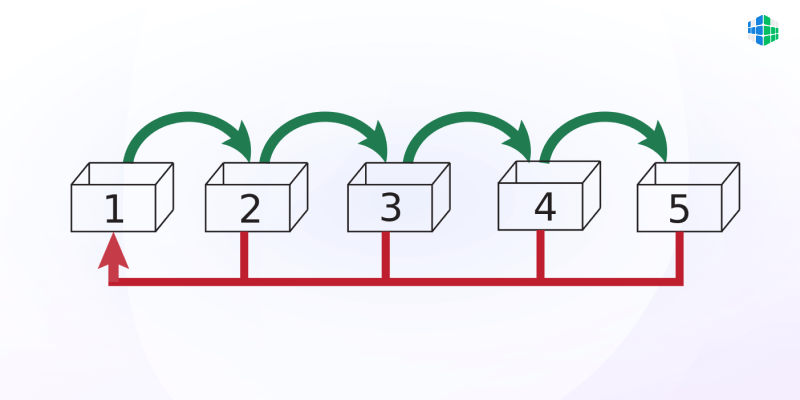
\includegraphics[width=0.49\textwidth]{img/sistema-lejtnera.png}
    \end{center}
    \caption{Система Лейтнера: 5 шагов, позволяющих выучить что угодно}
\end{wrapfigure}
Как часто вам приходится жаловаться на память? Как часто вам нужно что-то запомнить, а оно никак не запоминается? И как быстро вам надоедает все это повторять настолько, что вы решаете обойтись без этих знаний?

С подобной ситуацией сталкивается около 80\% людей, изучающих, например, иностранный язык. И как раз в помощь им была создана система Лейтнера. Однако впоследствии оказалось, что она пригодна для запоминания любой другой информации. Что же это за система такая?

\textbf{Волшебные карточки Лейтнера}

Основой системы Лейтнера являются так называемые флэш-карточки, на которых записывается информация для запоминания. Карточки могут быть обычными бумажными либо электронными.

За основу бумажной версии можно взять обычные каталожные карточки, которые можно увидеть в любой традиционной библиотеке, где есть каталоги – алфавитный, систематический, топографический. Как вариант, можно вырезать карточку удобного лично вам размера из плотной бумаги или тонкого картона.

Лайфхак для офисов и издательств – не выбрасывайте оставшиеся невостребованными карманные календарики за прошлый год. На светлом фоне можно писать черным маркером, а такие карточки будут выглядеть интереснее и веселее, чем обычные, сделанные из одноцветной бумаги.

Электронные карточки можно сделать в любом мобильном приложении для создания заметок или же воспользоваться специальным софтом. Для русскоговорящих пользователей можно рекомендовать мобильное приложение Brainscape или онлайн-программу Quizlet, также имеющую версии для iOS и Android.

Принцип использования бумажных и электронных карточек идентичен. Разница лишь в том, каким способом вы будете «тасовать колоду»: перелистывая экран или перекладывая карточки из одной стопки в другую.

\textbf{Как пользоваться карточками}

Каждый из нас замечал, что даже самое банальное «не получается» имеет свои градации: не очень получается, не всегда получается, не получается от слова «совсем». Если воспользоваться традиционным линейным способом заучивания, весь материал придется проходить каждый раз от начала до конца, будь то список новых слов по английскому, набор формул по физике или даты исторических событий.

Система Лейтнера позволяет не тратить время на повторение уже выученного материала, даже если он идет в связке с пока неизученным. Эта система удобна тем, что можно сосредоточиться только на том, что пока никак не запоминается, и регулировать частотность повторений по мере усвоения. Как это работает?



Алгоритм использования флэш-карточек:
\begin{enumerate}
    \item Распределяем весь изучаемый в данный момент материал по карточкам в режиме 1 карточка = 1 единица информации.
    \item Карточки с информацией, которую не получается запомнить совсем, складываем в первую колоду и повторяем ежедневно.
    \item Карточки с информацией, которую вы помните фрагментарно, помещаете во вторую колоду и повторяете через день.
    \item Карточки с информацией, которую вы иногда забываете или не всегда можете быстро вспомнить, помещаете в третью колоду и повторяете раз в три дня.
    \item По мере освоения материала карточки из первой колоды перекладываете во вторую, а затем в третью колоду.
\end{enumerate}

Такой подход называется методом интервальных повторений, т.е. повторений с определенными оптимальными для достижения результата интервалами. Не обязательно перечитывать всю колоду за один раз. Прочитайте столько, сколько успеваете, пока едете на работу, стоите в очереди, помешиваете кашу на медленном огне. Таких «бесполезных пятиминуток» может быть несколько в течение дня, и в сумме набегают те же 45 минут, что нужны для полноценного урока.

Теперь чуть подробнее о единицах информации. Это может быть, например, слово на английском – транскрипция – перевод на русский. Или формула по физике с расшифровкой переменных, внесенных в формулу. Или дата и название исторического события. Такой подход идеален для школьников в возрасте до 12-13 лет, которым сложно воспринимать сразу большой объем сведений.

Студенты, старшеклассники и взрослые могут расходовать площадь карточки более экономно и записывать на одну карточку сразу 2-3 связанные единицы информации. Например, три формы глагола в английском, две формулы из раздела «Кинематика» для расчета средней скорости движения и средней скорости при неравномерном движении, даты первого, второго и третьего раздела Польши в 18 столетии. Само собой, для трансфера карточки в следующую колоду нужно освоить все слова, формулы, даты с карточки.

К слову, при использовании электронных карточек вы можете получать рекомендации, сколько времени вам потребуется для запоминания той или иной информации и как часто нужно ее повторять. В частности, эта функция есть в приложении Brainscape. Вам требуется на старте самостоятельно оценить свой уровень знаний по каждой карточке от 1 до 5, и приложение выдаст свои рекомендации для дальнейшего изучения материала.

Английский, физику и историю мы взяли исключительно для примера. На самом деле, область применения карточек намного шире.

\textbf{Область применения системы Лейтнера}

Мы начали с того, что изначально данная система была разработана Лейтнером для изучения иностранного языка. Себастьян Лейтнер был журналистом, поэтому знание языков было для него профессиональной необходимостью.

Процесс изучения языка был адаптирован под существующие обстоятельства, т.е. высокую мобильность профессии журналиста, когда из-за постоянных разъездов и командировок не получается выделить фиксированное время для занятий.

Набор флэш-карточек с новыми словами, формами глаголов, местоимений, причастий, деепричастий всегда можно взять с собой. Небольшой набор легко поместится в карман мужского пиджака, а две-три стопки не займут много места в сумке. К слову, для изучения иностранных языков можно приобрести готовые карточки.

Точно так же с помощью флэш-карточек можно готовиться к экзамену по любому предмету в школе и вузе, докладу на семинаре или конференции, запоминать расположение нот и варианты аккордов на грифе гитары, разучивать длинную песню, разделив ее на куплеты, бридж и припев, а в особо сложных случаях переписав на карточки построчно.

Так же с помощью карточек можно развивать память и остроумие, поместив на них короткие шутки, анекдоты, изречения по разным поводам. Если регулярно повторять шутки и анекдоты, которые имеют свойство забываться, через какое-то время ваш мозг будет моментально реагировать на подходящую ситуацию, где можно блеснуть остроумием и выдать актуальный юмор.

Многим эта система так нравится, что они готовы заменить ею весь учебный процесс. Стоит ли это делать? Давайте подумаем.

\textbf{Система Лейтнера: в придачу или вместо?}

Тут хочется вспомнить известную поговорку: все хорошо в меру. Конечно же, система Лейтнера не может полностью заменить лекции, семинары и уроки хотя бы потому, что на семинарах и лекциях можно получить обратную связь преподавателя.

Разумеется, система Лейтнера не может заменить систематизированный курс по какой-либо специализации, будь то приемы оказания первой медицинской помощи или основы компьютерной грамотности. Карточки лишь носители единиц информации, а полностью овладеть знаниями можно, только когда вы получаете систематизированный курс лекций в нужной последовательности и учитесь применять полученные сведения на практике.

По этой же причине система не может стать альтернативой получению среднего или высшего образования, даже если на карточки перенести все формулы и даты по всем предметам. Однако система Лейтнера может существенно дополнить традиционные методы обучения, облегчить процесс усвоения и сэкономить время на изучение материала.

Как было сказано выше, пользование флэш-карточками вовсе не требует выделения фиксированного времени в вашем распорядке дня, и вы можете заполнить карточками любой пустой отрезок дня, когда не предвидится ничего более важного и интересного.

Если такой не заполненный полезными делами промежуток времени оказался слишком большим, вы можете повторить информацию из всех трех колод, а потом пойти по кругу, вернувшись к первой стопке. Это будет исключительно вам на пользу и станет отличной проверкой функциональности вашей кратковременной памяти. Вы сами сможете увидеть, с какой скоростью вы запоминаете или забываете информацию и, возможно, откорректировать методы самообразования в дальнейшем. Теперь подытожим все преимущества системы.

Преимущества системы Лейтнера:
\begin{enumerate}
    \item Простота и доступность.
    \item Возможность реализовать в бумажном или электронном формате по выбору.
    \item Возможность использования везде и всюду.
    \item Применимость для разных областей знания.
    \item Пригодность для подготовки к экзаменам по любым предметам.
    \item Пригодность для запоминания любой информации, которую можно разбить на короткие логические блоки.
    \item Развитие памяти – оперативной, среднесрочной и долгосрочной.
\end{enumerate}

К слову, с развитием памяти и техник запоминания информации вам может помочь наш курс «Мнемотехники», где вы освоите полезные лайфхаки, как быстро и надежно запоминать имена, даты, лица, термины, иностранные слова и все, что вам нужно. В качестве бонуса по окончании курса вы получите новый уровень развития ассоциативного мышления и научитесь придумывать рифмы к любым словам, требующим запоминания.

Так что желаем вам свежих знаний, полезных сведений, новой информации и ждем вас на нашем курсе, где научим все это запоминать. Поделитесь ссылкой на курс у себя на страничке в соцсетях – так вам будет легче вспомнить, где именно стоит искать этот курс, когда вы будете готовы начать учиться. Удачи!

\clearpage
\section{Метод изучения языков Китайгородской}

\textit{Источник: \url{https://4brain.ru/}}

\begin{wrapfigure}{l}{0.5\textwidth}
    \begin{center}
        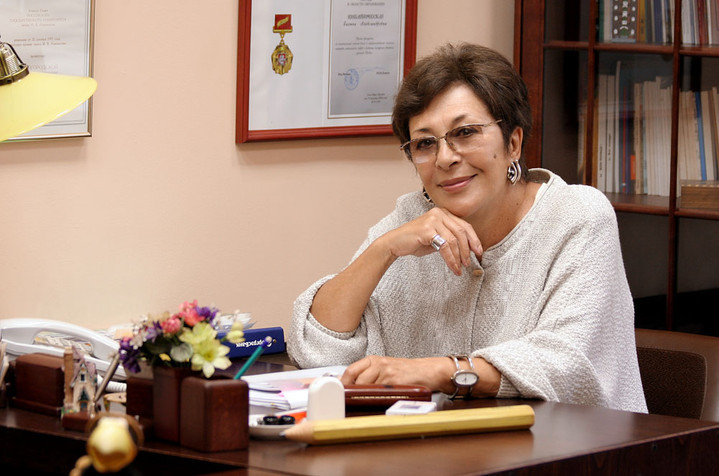
\includegraphics[width=0.49\textwidth]{img/kitaigorodskoi.jpg}
    \end{center}
    \caption{Китайгородская, Галина Александровна}
\end{wrapfigure}
С каждым днём в сфере образования появляются какие-то новые \ed{разработки}{разработка}{development}, программы, \explain{обучающие методики}{teaching methods} и другие всевозможные \ed{н\'{о}вшества}{н\'{о}вшество}{innovation}. Старые, же, или, как ещё их можно назвать, традиционные, если уж и не забываются, то просто отодвигаются на задний план по причине потери своей \ed{актуальности}{актуальность}{relevance} и малой эффективности. И эта тенденция наблюдается во всех направлениях, по которым происходит обучение, в том числе и в изучении иностранных языков.

Большинство традиционных методик обучения иностранным языкам сейчас \explain{подвергается}{undergoes; is subjected to} жёсткой критике, т.к. многие специалисты считают, что обучать им современных детей, да и взр\'{о}слых тоже, следует по ин\'{о}му пут\'{и}. А представление о прив\'{ы}чных мет\'{о}диках обучения складывается прим\'{е}рно такое:
\begin{enumerate}
    \item Огромное количество тр\'{у}дных грамматических правил, которые необходимо заучивать
    \item Десятки листов со словами, которые также нужно заучивать
    \item Объёмные неинтересные тексты, которые нужно читать, переводить и пересказывать
\end{enumerate}

Как вы сами считаете, нужно ли продолжать применять такие м\'{е}тоды в современных образовательных учреждениях? Наверняка, вы скажете, что лучше найти нечто более интересное и эффективное, что оказывало бы на учащихся большее стимулирующее воздействие, и помогало бы им гораздо быстрее осваивать лексику, грамматику и фонетику того языка, который они изучают.

И на сег\'{о}дняшний день исследователи \explain{выделяют}{identify} два основн\'{ы}х инновационных пути изучения языков, которыми являются:
\begin{enumerate}
    \item Применение методов изучения иностранных языков, осн\'{о}вывающихся на эффекте сверхзапоминания, когда восприятие и усвоение информации происходит без её критического осмысл\'{е}ния;
    \item Применение нетрадиционных методов, которые подразумевают ускоренное и максимально интенсивное обучение иностранному языку, где теоретическая база является минимальной или её вообще нет, а \explain{основной уп\'{о}р}{main emphasis} д\'{е}лается на практике, т.е. на разговорной речи в процессе жив\'{о}го общения.
\end{enumerate}

Базой об\'{о}их этих путей являются принципы суггестологии, которые б\'{ы}ли разработаны болг\'{а}рским педагогом и псих\'{о}логом Геогрием Лозановым. Ст\'{о}ит сказать, что суггестология является наукой, посвящённой раскрытию скрытого потенциала человека, и активизирующей его подсознательные ресурсы. В качестве примера можно назвать м\'{е}тод всем известного «25 кадра», а также обучение во сне. И как раз одним из м\'{е}тодов обучения иностранным языкам, которые основываются на принципах суггестологии, является метод Галины Александровны Китайгородской.

\textbf{Метод Г. А. Китайгородской}

Метод Г. А. Китайгородской, который также называют м\'{е}тодом «Активизации рез\'{е}рвных возможностей личности и коллектива», нельзя назвать новым, т.к. он был разработан свыше 35 лет назад, однако он считается исключительно \ed{нов\'{а}торским}{нов\'{а}торский}{innovative} и уже ставшим классическим в области интенсивного обучения.

Важно также сказать, что именно Галиной Александровной Китайгородской была создана единственная в России научная система интенсивного обучения иностранным языкам, а также был введён сам термин «интенсивное обучение». И с момента создания этой системы её эффективность была оценена огромнейшим количеством людей, которые в рек\'{о}рдно короткие сроки овладели иностранными языками.

Отличие м\'{е}тода Китайгородской от традиционных заключается в том, что он \explain{з\'{и}ждется}{is based on} на психологических резервах личности и коллектива при \ed{целенаправленной}{целенаправленный/-ая}{purposeful; targetted} манипуляции социально-психологическими процессами \ed{межличностного}{межличностный}{interpersonal} группового взаимодействия, благодаря чему учащиеся за совершенно мизерное время очень легко и продуктивно перерабатывают большие объёмы новых знаний.

Ключевое место в системе интенсивного обучения занимает термин «активизация» --- процесс, который направлен на достижение человеком активности и стабилизацию данного состояния. В своей изначальной интерпретации понятие «интенсивность» рассматривается как «напряжённость», а именно: состояние активности в конкретный момент времени. Точно также следует и трактовать понятие «интенсивного обучения» в рамках системы Г. А. Китайгородской – оно должно пониматься как динамизм, активное взаимодействие педагогов и группы учащихся, учащихся друг с другом, активизация процессов \ed{познания}{познание}{knowledge; cognition}, ресурсов памяти, воображения и внимания.

Тот ученик, который устал, засыпает на занятиях и нисколько не заинтерес\'{о}ван в своём обучении, не способен \explain{надлеж\'{а}щим \'{о}бразом}{properly} воспринимать большие объёмы информации и \explain{всецело}{wholly; entirely} отдаваться общению со своими партнёрами по обучению. А методика Китайгородской спос\'{о}бна привести учащегося в такое состояние, в котором он будет максимально \explain{\'{у}мственно}{mentally} и нередко даже физически активен, по причине чего будет обесп\'{е}чен самый высокий показатель интенсивности процесса обучения. Если говорить несколько проще, путь овладения человеком иностранным языком, согласно системе Китайгородской, очень \explain{схож}{similar} с тем путём, идя по которому ребёнок осваивает свой родной язык.

Сначала учен\'{и}к двигается вперёд по различным стадиям формирования способности к речи, начиная с интонационной, затем переход\'{я} к лексико-грамматической, а после --- к синтаксической и фонетической. Причём, происходит всё это совершенно естественным образом, а не наоборот, как это можно наблюдать в традиционных м\'{е}тодах обучения. И сроки овладения новым навыком значительно сокращаются.

Уже в процессе первого занятия ученик начинает \explain{изъясняться}{(here) to speak} на иностранном языке при помощи готовых конструкций. \ed{Изначально}{изнач\'{а}льно}{initially} он, конечно, не знает правил грамматики, но постепенно переходит на уровень анализа тех конструкций, которые применяет, а потом снова начинает использовать их в своей речи, вместе с этим производя решение всевозможных задач в атмосфере естественного общения, но уже на совершенно другом уровне. Это называется микроциклом. И уже только на одном этапе процесса обучения этих микроциклов присутствует масса. В итоге ученик осваивает несколько тысяч лексических единиц в течение одного курса, но наиболее важно то, что он научается легко и непринуждённо применять их в различных ситуациях общения.

Всего за восемь недель обучения учащиеся начинают изъясняться на иностранном языке, снимают языковые барьеры, раскрепощаются и получают мощнейшую мотивацию к дальнейшему освоению языка. И этому в немалой мере способствуют специализированные учебники, предназначенные для каждого конкретного языка и каждого уровня обучения, должным образом организованное взаимодействие в группе учеников, атмосфера дружелюбия и творчества, интересные для выполнения задания, которые вызывают у учащихся желание их выполнять, уникальный психотерапевтический эффект, к достижению которого стремятся педагоги Школы Китайгородской, и множество других \ed{немаловажных}{немаловажный}{important} факторов.

\explain{В дополнение к этому}{In addition to this}, следует сказать, что с\'{о}зданная более 35 лет назад Галиной Александровной Китайгородской система обучения иностранным языкам в настоящее время актуальна и \explain{востр\'{е}бована}{in demand} гораздо больше, чем когда-либо вообще. И в качестве заключения несколько слов о Школе Китайгородской.

\textbf{Школа Китайгородской}

Школа Китайгородской является единственным в нашей стране научно-образовательным центром, в котором научные и практические м\'{е}тоды напр\'{а}влены на достижение единого результата --- интенсивного обучения людей общению на иностранных языках.

Данное научно-образовательное учреждение было основано в 1985 году на базе открывшегося в 1979 году при Московском государственном университете им. М. В. Ломоносова Центра интенсивного обучения иностранным языкам.

Сегодня в Центре интенсивного обучения иностранным языкам пров\'{о}дится обучение для студентов и преподавателей МГУ им. М. В. Ломоносова, а в самом научно-образовательном центре «Школа Китайгородской» имеют возможность проход\'{и}ть обучение все, кто желает овладеть иностранными языками.

И уникальность Школы Китайгородской заключается вот в чём:
\begin{enumerate}
    \item Только в Школе Китайгородской иностранные языки преподаются по \'{а}вторской мет\'{о}дике интенсивного обучения, разработанной Г. А. Китайгородской, защищённой докторской диссертацией и описанной многими монографиями, методическими пособиями и статьями.
    \item Система интенсивного обучения Г. А. Китайгородской \ed{снабжен\'{а}}{снабжён, снабжен\'{а}}{is equipped} \'{а}вторскими учебниками, специально разработанными для каждого из уровней.
    \item Преподавательский \explain{сост\'{а}в}{staff} Школы Китайгородской \explain{состо\'{и}т из}{consists} лучших учеников-последователей профессора Г. А. Китайгородской, которые великолепно владеют мастерством педагогики.
\end{enumerate}

Школа Китайгородской всегда верна своей специфике и сохраняет неизменное высшее качество обучения иностранным языкам, которое основано на многолетнем опыте, множестве экспериментов и исследований.

\clearpage

\section{Активизация возможностей личности и коллектива}

\textit{Источник: \url{https://kitaygorodskaya.ru/method}}

М\'{е}тод «Активизация возможностей личности и коллектива» (Метод Китайгородской) --- это уникальная система обучения, защищённая д\'{о}кторской диссертацией, оп\'{и}санная в монографии, метод\'{и}ческих пос\'{о}биях и стать\'{я}х. Это инновация, ставшая классикой интенсивного обучения.

В течение многих лет нашей научной базой являлся Центр Китайгородской в МГУ им. М.В. Ломоносова.
Несколько десятков лет наш Метод работает на обучение жив\'{о}й разговорной речи. Уникальность Метода Китайгородской состо\'{и}т в том, что благодаря научно разработанной системе, используемым техникам запоминания и специально созданным учебникам результат достигается в кратчайшие сроки.

\textbf{Что же такое интенсивное обучение?
}

Чтобы точно определить, что является для нас главным в концепции так называемого интенсивного обучения, следует ввести слово «активизация». Активизация --- процесс, направленный на достижение активности личности и сохранение этого состояния. В своем исходном значении\footnote{in its original meaning} слово «интенсивный» (лат. "intensus") означает «напряжение», т.е. активность в единицу времени. В этом случае понятие «интенсивное обучение» соответствует нашей концепции --- динамизм, активность во взаимодействии преподавателя и уч\'{е}бной группы, учащихся между собой. Именно состояние активности преподавателя и учащегося обеспечивает высокий уровень интенсивности (активности) учебного процесса.

Подобное представление об обучении исключительно актуально, так как проблемы взаимодействия людей \explain{всё более}{more and more} \explain{прочно}{firmly, substantially} сращиваются с проблемами обучения иностранным языкам. Ведь сегодня стратегической целью обучения является не только овладение языком как средством общения, но и языком как средством \ed{приобщения}{приобщение + \textit{к}}{familiarisation} к иной культуре. Социопсихолингвистические исследования за рубежом и в нашей стране позволяют \explain{принимать за точку отсчёта}{take as a starting point} не языковой код, а речевую активность, активность речевой д\'{е}ятельности. Те\'{о}рия коммуникации \explain{убеждает}{convinces} нас в том, что недостаточно знать язык, систему языка, правила функционирования языкового кода. Чтобы общаться, надо знать, как п\'{о}льзоваться языком в определённом контексте, т.е. выучить язык означает сегодня овладеть речевым поведением в естественных ситуациях. В этих условиях функции языка, а не его структура, приобретают первостеп\'{е}нное значение в процессе обучения.

В нашей концепции интенсивного обучения мы рассматриваем овладение иноязычным общением в его устной и письменной форме с социально-психологических позиций. Общение на изучаемом языке \explain{прон\'{и}зывает}{pervades} процесс обучения, являясь одноврем\'{е}нно целью этого обучения, основным средством и условием его достижения. Поэтому интенсивное обучение может быть определен\'{о} как особым образом организованное обучающее общение, в ходе которого происходит \explain{уск\'{о}ренное}{accelerated} \explain{усвоение}{assimilation} материала (овладение предметом) и активное \explain{совершенствование}{improvement}, развитие личности (учащихся и преподавателя).

Естественно, что такое понимание интенсивного обучения исключает представление о «минимизации» учебного материала, а также усилий преподавателя и учащихся. В нашем случае речь иёт о максимизации объёмов учебного материала и усилий преподавателя и обучаемых, т.к. интенсивное обучение основано на активизации их деятельности. Активность участников учебного процесса выражается в максимальной и постоянной их вовлечённости в процесс управляемого группового взаимодействия, общения-обучения.

Широкое использование группов\'{ы}х (коллективных) форм взаимодействия в уч\'{е}бном процессе приводит к тесному \ed{переплетению}{переплет\'{е}ние}{weave; interlacing} методики и социальной психологии, что характеризует нашу концепцию интенсивного обучения. Это единственная психолого-педагогическая концепция, которая строит учебный процесс на основе принципа коллективного взаимодействия, «социального взаимодействия». Именно поэтому единицей организации учебного материала и учебной деятельности является ситуация взаимодействия, динамическое событие, моделирующее образы реальной жизни.

Итак, мы предлагаем иной психологический путь достижения педагогической цели. Психологические опоры интенсивного обучения требуют соответствующей организации учебного материала и учебного процесса.

Для более полного представления об интенсивном обучении необходимо остановиться на психолого-педагогических пр\'{и}нципах, которые не только характеризуют его, но и помогают преподавателю творчески использовать предлагаемое учебное пособие, оставаясь в рамках метода активизации возможностей личности и коллектива.

\textbf{Пр\'{и}нцип личностного-ориентированного общения}

Слово «общение» понятно всем, но может быть именно поэтому, когда это слово употребляется применительно к организации учебного процесса, то подчас возникает \explain{недоумение}{confusion; perplexity}: общение преподавателя с учениками, а тем более общение учеников между собой очень похвально, но на уроке мало времени, это слишком большая роскошь. Да и вообще, какое отношение имеет общение к обучению?

Попробуем ответить на этот вопрос с научной точки зрения. \explain{Общеизвестно}{It is generally known}, что личность формируется и функционирует в постоянном взаимодействии с другими людьми в основных видах деятельности: игр\'{е}, учёбе, труд\'{е}. Развитие личности учащегося протекает в двух взаимосвязанных деятельностях: учебной и общении. Известно также, что гармоничное развитие личности \explain{во многом}{in many ways} обеспечивается единством этих видов деятельности. Тенденция к \explain{слиянию}{merger} процессов обучения и общения характеризует современную педагогику и психологию обучения. \ed{Благоприятные}{благоприятный}{favourable} условия для достижения эффективных результатов открываются тогда, когда требования учебной задачи представляются обучаемому привлекательными, удовлетворяющими его потребности.

Чтобы создать необходимые для этого условия, надо построить учебный процесс таким образом, чтобы отношение к изучаемому предмету формировалось через отношение к другому человеку (соученику, учителю), а оно, в свою очередь --- через групповое взаимодействие, иными словами, необходимо обеспечить максимальное слияние общения и обучения. Именно в этом случае, по утверждению психологов, общение выполняет обучающую и развивающую функции и приводит к наиболее продуктивному овладению изучаемым предметом при одновременном всестороннем личностном развитии. Все это, как нам кажется, дает основание для введения понятия обучающего общения.

\textit{Почему же мы формулируем этот принцип как принцип личностного общения?}

Прежде всего, в понятие «личностное» мы вкладываем психотерапевтическое и психологическое содержание: \explain{доверительность}{confidence}, поддержка, \explain{доброжелательность}{kindness; benevolence}. Ведь общение, диалогическое общение, с позиции социальной психологии подразумевает установление отношений взаимного доверия, откровенности. В диалоге (в широком смысле слова) представлены голоса всех его участников, что позволяет \explain{сопоставлять}{compare; contrast; juxtapose} различные точки зрения, определять свою собственную и рассматривать ее как одну из возможных.

Диалогическое общение в таком расширительном понимании предполагает организацию особого типа отношений его участников, характеризующихся \ed{устремлённостью}{устремлённость}{aspiration; tendency; desire} к другому человеку, вниманием и интересом к нему, способностью \ed{дорожить}{дорожить кому-то}{высоко ценить что-либо, придавать большое значение чему-либо} другим человеком, видеть в нем цель, а не средство. Взаимный характер общения приводит к активной позиции каждого его участника. Однако надо помнить, что одно из важнейших умений в общении --- умение слушать собеседника. Для преподавателя интенсивного обучения это особо важное качество, т.к. он должен уметь строить общение в учебной группе по типу реального общения, «вплетая» в этот контекст неформального личностного общения учебный материал (упражнения).

\textit{Принцип личностного общения.}
Реализация этого умения на практике означает, например, что, задав вопрос, преподаватель должен уметь выслушать своего ученика не только и не столько как «ученика», но и как собеседника, партнера. Это умение \explain{проявляется}{is manifested} в реакции на содержание, смысл сказанного учеником.

Преподаватель не стремится оценить ответ ученика, что так привычно в педагогической практике. Он выражает, высказывает свое отношение к содержанию сообщения. Это невероятно важно, т.к. именно выражение своего отношения к сказанному учеником выводит эту учебную ситуацию за рамки формального взаимодействия, превращает учебное общение в неформальное личностное, т.к. позволяет «вплести» тренировку учебного материала (упражнения) в контекст реального общения.

Организация такого обучающего общения требует от преподавателя специальных умений и определенных усилий, особенно на начальном этапе, когда ученик еще очень ограничен в выборе языковых средств и, кроме того, в сознании учащегося (да и преподавателя) действует стереотип учебного взаимодействия, созданный предшествующим опытом учения и преподавания. Этот стереотип держит преподавателя в рамках «опросной» системы, когда любой ответ, сообщение ученика замыкается на преподавателя, ответ которого заключает в себе оценку формальной стороны сообщения ученика. Необходимо сразу же преодолевать этот стереотип, и с этой точки зрения чрезвычайно важным оказывается использование специального приема, который мы называем «передачей», «перепасовкой» реплики (ответа, сообщения) одного учащегося другим (группе), стимулируя тем самым их собственные высказывания, реакции, активность в поддержании и развитии диалога в группе. Преподаватель \explain{ос\'{о}знанно}{consciously} стремится не принимать все реплики учащихся «на себя», отдавать их, как мяч в волейболе.

\textit{Как организовать личностное общение?}

Успешность в организации личностного общения на занятиях зависит от того, как \explain{отобран}{selected $<$ отбирать/отобрать: to choose; to select; to single out} и организован учебный материал. Так, например, отбор учебного материала обязательно предусматривает наличие специальных языковых средств для вступления в контакт, для выхода из контакта и т.п., всего того, что позволяет обучаемому выражать себя как личность в организованном и управляемом преподавателем иноязычном общении. Организация учебного материала в жизненно значимых ситуациях, комбинации которых заложены в текстах-полилогах, служит моделью личностного общения, помогая обучаемому в дальнейшем находить речевые способы и средства решения многих других однотипных ситуаций, отталкиваясь от имеющегося образца.

Не только отобранный учебный материал, представленный в текстах-полилогах, не только система коммуникативных упражнений, основой которой является принцип личностного общения, но и такие характеристики, как количество обучаемых, состав группы и ее пространственное расположение, подчинены принципу личностного общения. Оптимальный объем группы --- 12 человек, состав гетерогенный, что позволяет создать в группе репрезентативную модель общества, расположение в аудитории --- полукругом, лицом к лицу. Эти параметры, кстати, характерны для всех групповых форм психологической работы (Т-группы, группы тренинга умений, психодрама и т.д.).

\textbf{Принцип игровой/ролевой организации учебного материала и учебного процесса}

Наблюдения за учебным процессом в средней и высшей школе, особенно за обучением иноязычному общению, показывают, что одна из серьезных причин очень малой эффективности заключается в низком уровне мотивированности обучаемого. Большей частью преподаватель предлагает учащимся псевдокоммуникативные задания типа: «Пригласите соседа в гости», «Узнайте, как доехать до...». Речевые действия учащихся при выполнении подобных заданий не мотивированы, и значит --- формальны. Эти задания не многим отличаются от заданий типа: «Перескажите текст», «Переведите предложение» и т.п. В них нет ответа на главный вопрос, возникающий у обучаемого, --- «Зачем, с какой целью я должен это сделать, сказать?».

\textit{Принцип ролевой организации.}
Вероятно, для \explain{устранения}{elimination} этого недостатка следует прежде всего осознать важное место ролевого поведения в учебной деятельности учащихся. Опыт интенсивного обучения иностранным языкам позволяет \explain{сделать вывод}{to draw a conclusion} о больших возможностях ролевого общения (ещё далеко не полностью исследованных) и целесообразности его использования в обучении.

Эта идея поддерживается лингвистами, которые видят в ролевом общении эффективный способ приобретения речевой компетенции, и психологами, \explain{утверждающими}{которые утверждают $<$ утверждать/утвердить: to assert, to argue, to allege, to state; to claim; to approve. Here: ``who argue''}, что приёмы организации ролевого общения напр\'{а}влены на приведение в действие механизмов мотивации. Ролевое общение на иностранном языке в условиях интенсивного обучения --- это не фрагмент занятия, не методический прием, не упражнение, а основа построения учебного процесса. Обучать иноязычному общению (в его устных и письменных формах) можно лишь в \ed{непрерывном}{непрерывный}{continuous, uninterrupted} личностно-ролевом взаимодействии.

Ролевое учебное общение в интенсивном обучении предполагает постоянную активность субъектов общения (всех учащихся и преподавателя), которые не ограничиваются просто восприятием сообщения и реакцией на него, а стремятся выразить свое отношение к полученной информации. Специфика ролевого учебного общения заключается в том, что оно сохраняет все социально-психологические характеристики истинного общения. Поэтому общение является для обучаемого целью его речевого (или неречевого) действия в условиях, максимально приближенных к неучебной \ed{совместной}{совм\'{е}стный}{joint} деятельности. Для преподавателя же это общение является и учебным, поскольку ситуации общения (упражнения) им планируются и организуются.

Преподаватель управляет общением при решении конкретных учебных задач, необходимых для реализации целей курса обучения. Таким образом, с позиции преподавателя, ролевая игра, ролевое общение --- форма организации учебного процесса, а с позиции учащихся --- коммуникативная, познавательная, игровая деятельность. Увлеченный решением сменяющих друг друга коммуникативных задач в общении с различными партнерами, обучаемый большей частью не осознает учебной стороны решаемых задач. Исключение составляют чисто познавательные, аналитические задачи, но и они преподносятся в форме, поддерживающей интерес учащихся. Организованная как личностное общение, учебная деятельность протекает в форме общения-игры.

Важно \explain{напомнить}{to remind}, что игра понимается нами в широком смысле слова --- как форма \ed{непосредственного}{непосредственный}{direct, immediate}, но \ed{продуманного}{продуманный}{well thought-out} и управляемого общения преподавателя и группы. Кстати, неправильное понимание игры --- одна из причин больших трудностей при овладении профессией преподавателя интенсивного обучения.

\textit{Что же такое игра?}

На этот вопрос наиболее \explain{чётко}{clearly} отвечают психологи, определяя игру как важный тип и уровень функционирования личности взрослого человека, как условие сохранения его психического здоровья и \ed{полноценной}{полноценный}{full-fledged} \explain{созидательной}{созидательный}{creative, constructive} деятельности. Главное, чтобы предлагаемые ролевая игр\'{а}, ролевое общение были по своему содержанию на соответствующем обучаемому контингенту интеллектуальном уровне. К сожалению, примитивное понимание преподавателем игры, игровой деятельности иногда приводит к «детским играм», примитивным коммуникативным задачам, т.е. к снижению интеллектуального творческого уровня обучения.

\textit{Как же преподаватель организует ролевое общение и управляет им?}

Прежде всего, преподаватель организует непрерывное общение через решение множества коммуникативных задач, представленных в коммуникативных упражнениях. При подготовке к занятию преподаватель создает упражнения для решения конкретных учебных задач на определенном языковом и речевом материале, а затем комбинирует их в сценарии занятия. Коммуникативные задания в упражнениях формулируются как естественные жизненные ситуации, исходя из конкретного языкового и речевого материала, который запланирован преподавателем для определенного этапа его отработки.

Принцип ролевой организацииТрудно переоценить методическое значение роли. Роль является одним из главных средств обеспечения мотивированных многократных повторений учащимся одних и тех же языковых и речевых единиц, что необходимо для формирования речевого навыка. Но и психологическое, психотерапевтическое значение роли огромно.

Учащийся в зависимости от типа своей личности, от степени владения изучаемым языком, от конкретной роли в данной ситуации может «самовыражаться», творчески реализовывать свои знания, умения, свой интеллектуальный потенциал, а может «прятаться за свою роль», т.е. минимальными языковыми средствами и, как правило, широко привлекая невербальные средства, «создавать свою роль» как средство защиты. Преподаватель же продуманно \ed{вовлекает}{вовлекать/вовлечь}{to involve} каждого в общую деятельность, распределяет роли в ситуации, делает временным лидером каждого, одним словом, управляет общением, учит общаться.

Роли-легенды, заложенные в тексте-полилоге, и ситуации полилога реализуются в учебном процессе лишь при введении текста-полилога и, частично, на первом занятии тренировки в общении. На всех остальных занятиях преподаватель «работает» на ситуациях-вариантах при использовании самых различных ролей и масок, что позволяет отрабатывать необходимый языковой и речевой материал в большом количестве разных ситуаций.

Постоянная смена ролей и ситуаций на занятиях способствует поддержанию мотивации речевых действий учащихся при большом количестве повторений одних и тех же языковых единиц и грамматических явлений, что является необходимым условием для формирования прочного и \ed{гибкого}{гибкий}{flexible} речевого навыка. Третий принцип --- коллективное взаимодействие --- основной психологический принцип, на котором построено интенсивное обучение. Суть его --- организация групповых (коллективных) действий, способствующих внутренней мобилизации возможностей личности обучаемого.


\textbf{Принцип коллективного (группового) взаимодействия}

Принцип коллективного взаимодействия определяет такой способ организации учебного процесса, при котором:
\begin{enumerate}
    \item учащиеся активно общаются друг с другом, обмениваясь учебной информацией, расширяя за счет этого свои знания, совершенствуя умения и навыки;
    \item между участниками складываются благоприятные взаимоотношения, служащие условием и средством эффективности обучения и творческого развития каждого;
    \item условием успеха каждого является успех остальных.
\end{enumerate}

Таким образом, активное общение преподавателя с учащимися и учащихся между собой является социально-психологическим фактором успешности процесса обучения, одновременно обеспечивая эффективность формирования познавательных действий и приемов общения на изучаемом языке. Совместные действия и межличностные отношения в системе учитель-ученик, ученик-группа и т.д. являются также средством повышения продуктивности индивидуальной деятельности ученика.

В активном взаимодействии друг с другом учащиеся не только обмениваются знаниями о системе языка, когда, помогая друг другу, дают языковые комментарии, объясняют правила своему партнеру, но и учатся общаться. Процесс обучения иноязычному речевому общению --- это двусторонний процесс, в котором многое приобретает не только учащийся, но и учитель.

Организуя иноязычное общение и управляя им в группе, он совершенствует свои коммуникативные умения. В ходе взаимодействия с учащимся \explain{уточняется}{refines} его собственное \explain{представление о себе}{self image}, становится более адекватной самооценка.

\textbf{Типы учебного взаимодействия }

Особую значимость приобретает вопрос о типах учебного взаимодействия. Типы и способы учебного взаимодействия должны обеспечивать постоянную и активную \explain{вовлечённость}{involvement} учащихся в процесс обмена информацией. В нашей методической системе используются многие способы учебного взаимодействия, дополняющие друг друга и придающие учебной деятельности коллективный характер: одновременная работа в парах (диадах); одновременная единая или дифференцированная работа в триадах; одновременная единая или дифференцированная работа в микрогруппах по 4 человека; работа в командах (2 микрогруппы); учащийся-группа; преподаватель-группа; преподаватель-микрогруппа и т.д.

В интенсивном обучении чрезвычайно усиливается активность учащегося, так как на протяжении всего занятия он решает попеременно с другими учениками поступающие одну за другой от преподавателя коммуникативные задачи. В результате, благодаря его усилиям, сознательно регулируемым преподавателем, конструируется такая система отношений, которая позволяет как можно полнее раскрыть, использовать и развить возможности каждого.

Развитию творческой индивидуальности обучаемых в коллективной учебной работе способствуют:
\begin{enumerate}
    \item \explain{доверительные отношения}{trusting relationships} между преподавателем и учащимися, которые освобождают учащихся от \ed{скованности}{ск\'{о}ванность}{(lit) inhibition; stiffness} и чувства неуверенности в себе;
    \item поощрения со стороны преподавателя и товарищей по группе, помогающие обучаемому поверить в свои силы;
    \item идентификация обучаемого с группой;
    \item организация учебной деятельности в совместных игровых формах;
    \item организация учебной деятельности в форме серий заданий, интересных для обучаемых и предполагающих их активное взаимодействие.
\end{enumerate}

\textbf{Роль преподавателя }

Организация речевого общения в условиях коллективной познавательной деятельности предполагает особую роль преподавателя. Речь идет о таком типе педагогического общения, который \explain{бл\'{и}зок к}{close to} оптимальному --- развивающему и \ed{взаимообогащающему}{взаимообогащающий $<$ обогощать/обогатить (\textit{что, чем}): to enrich (e.g., обогащать ум знаниями)}{mutually enriching} человеческому общению. Поэтому понятие профессионализма преподавателя требует \ed{пересмотра}{пересмотр}{revision}, включения в него особых педагогических способностей, связанных с реализацией коллективных форм сотрудничества как преподавателя с обучаемым, так и обучаемых между собой.

Вероятно, наш метод по своей методологической природе более элитарен по отношению к педагогам, \ed{предъявляя}{предъявляя}{presenting (предъявлять)} повышенные требования к их профессиональным и человеческим качествам. Ну что ж? Может быть и хорошо, что преподавать по этому методу не каждый сможет.

Коллективная познавательная деятельность, а также демонстрируемые преподавателем формы поведения, способствующие созданию атмосферы доброжелательности, взаимопомощи, внимательного отношения к партнерам, создают оптимальные условия для активизации возможностей каждого учащегося и развивают способность правильно воспринимать других и адекватно оценивать себя, свои \ed{поступки}{поступок}{action}, результаты своей деятельности.

Постоянное учебное взаимодействие с меняющимися партнерами дает возможность каждому правильно увидеть себя, оценить, прогнозировать поведение. На фоне положительной установки на восприятие каждого члена группы, которая сохраняется и развивается в ходе обучения, процесс формирования адекватной самооценки и уровня притязаний протекает быстрее.

\textbf{Принцип концентрированности в организации учебного материала и учебного процесса}

Концентрированность учебных часов является одной из внешних характеристик интенсивного обучения. Однако наличие этой характеристики еще не означает, что данное обучение --- интенсивное. Понятие концентрированности должно быть расширено, что позволит детерминировать специфику интенсивной системы обучения. В условиях интенсивного обучения, когда решаются задачи обучения устным и письменным формам иноязычного общения, как правило, за минимальные сроки, оказываются принципиально важными еще два фактора: количество (объем) учебного материала и его \explain{распределение}{distribution} в курсе обучения.

Увеличение объема учебной информации в курсе, \explain{предпринятое}{{undertaken}} ещё Г. Лозановым\footnote{Георгий Лозанов: болгарский педагог и психолог, разработавший в 1960-е годы метод суггестопедии, используемый для ускоренного обучения иностранным языкам.}, \explain{обусловлено}{is due to}, на первый взгляд, чисто внешними обстоятельствами --- \ed{сжатыми}{сжатый}{compressed} сроками обучения. Но такое понимание причин увеличения и концентрации материала было бы несколько \explain{упрощённым}{упрощённый}{simplified}. По с\'{у}ти, речь идёт о взаимозависимости двух факторов. С одной стороны, открывшиеся возможности активизации учебной деятельности создали предпосылки для успешного усвоения повышенных объемов концентрированной учебной информации. С другой стороны, концентрированность учебного материала оказывает активизирующее воздействие на познавательные процессы. Обучаемый как бы перестраивается на новый, более активный режим деятельности, который способствует максимальным \ed{проявлениям}{проявление}{manifestation} его творческих возможностей, в частности, возможности запоминать большие объемы информации без специального заучивания.

Концентрированность в организации учебного материала и учебного процесса находит своё \explain{воплощение}{embodiment} в предлагаемой нами трёх\'{y}ровневой модели овладения устными и письменными формами иноязычного общения «Синтез-Анализ-Синтез». Этапы овладения учащимися иноязычным общением по данной модели непосредственно связаны с объемом учебного материала и его распределением в курсе обучения.

При определении общего объема учебного материала мы исходим из максимума, необходимого для реализации целей курса обучения (в нашем случае 2000-2500 лексических единиц).

\textit{Первый этап} (С1) предполагает формирование у обучаемых коммуникативного \ed{ядр\'{а}}{ядр\'{о}}{core, nucleus},
практически обеспечивающего устные формы общения на относительно простом уровне. Для решения этой задачи необходимо овладение значительным объемом языкового материала (800-1200 л.eд.).
Большой объем учебного материала, сконцентрированный на первых семи-десяти занятиях курса, необходим для дальнейшего плодотворного осмысления учащимися
\explain{накопленного}{накапливать/накопить: to accumulate; накопленный: accumulated} ими речевого опыта, систематизации языковых явлений, т.е. следующего этапа --- анализа.
Именно большой объём материала, усвоенный на первом этапе обучения, создаёт базу для последующей самостоятельной аналитической д\'{е}ятельности учащихся и обеспечивает сравнительную лёгкость её протекания. \ed{Следует оговорить}{следует оговорить}{it should be specified},
что начальный этап обучения проходит в устной форме, т.е. без полной и постоянной зрительной опоры на текст (даже если обучаемые не «нулевого» уровня). \ed{Обильное}{обильный}{abundant} слушание, происходящее на этом этапе, развивает фонематический слух учащихся, языковую догадку, дает возможность обучаемому \explain{опознавать}{to identify, to recognise, to spot} в речи языковые формы в их оппозиции, в сопоставлении и различном окружении, что одновременно активизирует аналитические процессы.
Нельзя \explain{упускать из виду}{overlook} и ещё одно важное следствие: поступление больших объёмов учебного материала. Оно даёт возможность преподавателю организовывать ситуации, максимально приближенные к реальному общению, на первом же занятии, и тем самым с самого начала создавать высокую мотивацию учения.

\textit{Этап Анализа}, как \explain{промежуточный}{interim} этап, предполагает поступление меньших объёмов новой учебной информации, чем на этапе Синтез.

Однако, по сравнению с принятыми в практике обучения нормами, объём поступающей на этапе Анализа информации остаётся высоким. Материал продолжает поступать в концентрированном виде (большое количество новой учебной информации за одно предъявление). Этот этап необходим для перехода от репродукции речевых высказываний в данной ситуации и для данных целей (С1), к их активной продукции и ситуативному варьированию (С2). Третий этап предполагает поступление больших объемов лексической информации при практическом отсутствии нового грамматического материала.

Концентрированность в организации учебного материала, естественно, \explain{предопределяет}{determines} концентрированность в организации учебного процесса. Имеющиеся в тексте ситуации являются основой для множества других, которые включаются в коммуникативные упражнения для тренировки каждого лексико-грамматического явления на разных уровнях его отработки. Сменяя друг друга, вариативные упражнения создают насыщенность, «плотность общения» на занятии, обеспечивая постоянную речевую активность всех участников общения, всей учебной группы. А это, в свою очередь, позволяет\footnote{позволяет + кому} учащимся усваивать большие объемы материала.

Принцип концентрированности в организации учебного материала и учебного процесса недостаточно полно определял бы интенсивное обучение иностранным языкам, если бы мы не дополнили его понятием коммуникативной связанности. Коммуникативная связанность, которая понимается нами как интегрирующая функция коммуникативного взаимодействия, позволяет обеспечить овладение учащимися большими объемами материала, создавая легкость в восприятии новых учебных текстов, снимая монотонность и поддерживая мотивацию при отработке большого количества лексико-грамматических явлений. Коммуникативные связи --- это прежде всего смысловые связи. Именно текст-полилог, определяющий благодаря ролевой структуре взаимодействие участников коммуникации, в наибольшей степени насыщен коммуникативными связями, которые, в частности, выявляются в его лингвистических характеристиках.

Эти связи заложены в каждом новом учебном тексте-полилоге и проявляются в сюжете, который объединяет всю макроситуацию, раскрывающуюся в большом количестве (от 5 до 10) микроситуаций, связанных по смыслу и естественно вытекающих одна из другой в рамках правил коммуникации. Это позволяет учащемуся не только прогнозировать появление каждой следующей микроситуации, не только догадываться о каждой последующей реплике, но и создает смысловую коммуникативную канву, способствующую запоминанию всего текста-полилога.

Что же касается коммуникативной связанности в организации учебного процесса, то она обеспечивается контекстом общения преподавателя с группой. Именно контекст объединяет все упражнения, отобранные для одного занятия, в единое смысловое целое. Иначе говоря, создается сценарий занятия, который, как правило, не просто повторяет, а развивает в серии упражнений сюжет учебного текста. При этом преподаватель разрабатывает множество конкретных вариантов тех микроситуаций, которые заложены в учебном тексте, затем располагает их в определенной последовательности, диктуемой учебными задачами занятия, и, наконец, включает их в смысловой коммуникативно \explain{значимый контекст}{significative/meaningful context} своего общения с учебной группой. Таким образом, понятие коммуникативной связанности дополняет понятие концентрированности в организации учебного материала и процесса обучения.

\textbf{Принцип полифункциональности учебной деятельности и упражнений}

И, наконец, пятый принцип отражает специфику организации учебного процесса согласно модели овладения иноязычным общением (С1—А—С2). Это --- принцип полифункциональности упражнений. Данный принцип тесно связан с предыдущим, так как концентрированность и коммуникативная связанность в организации учебного материала и учебного процесса определяют специфику коммуникативных упражнений, а именно — их полифункциональность.

Полифункциональность упражнений соответствует тому подх\'{о}ду при обучении иностранному языку, который предполагает одновременное и параллельное овладение языковым материалом и речевой деятельностью, в отличие от традиционного подхода, предусматривающего последовательное овладение сначала языковым материалом, а затем --- речью. Поскольку приобретение навыков и умений иноязычного общения возможно лишь через непрерывное общение в ситуациях, моделирующих реальную коммуникативную деятельность, то единственно возможным в условиях интенсивного обучения является первый подход. Он описывается предлагаемой нами моделью овладения иноязычным общением (С1—А—С2).

На основе данной модели построена система упражнений-взаимодействий преподавателя и учащихся, учащихся между собой, опосредованных иноязычным материалом и определенными межличностными отношениями участников общения. Каждое коммуникативное упражнение одновременно решает несколько задач, представленных в определенной иерархической последовательности для каждого данного этапа обучения и данного этапа занятия.

Принцип полифункциональности упражнений строится на том, что выражение какого-либо коммуникативного намерения предопределяет выбор соответствующих грамматических форм, а каждая данная грамматическая форма требует адекватного для нее лексического наполнения. В организации упражнений это отражается следующим образом: тренировка употребления каждой данной грамматической формы осуществляется в серии упражнений, где в меняющихся ситуациях реализуется одно и то же коммуникативное намерение (например, сомнение можно выражать по разному поводу, в разных обстоятельствах, в разных ролях). При этом для учащегося любое упражнение монофункционально --- он решает коммуникативную задачу. Для преподавателя оно всегда полифункционально, так как он осознает необходимость решения нескольких задач в одном упражнении:
\begin{enumerate}
    \item тренировки в решении какой-либо коммуникативной задачи;
    \item тренировки в употреблении грамматической формы;
    \item тренировки в лексике;
    \item тренировки в фонетике.
\end{enumerate}

Причем в зависимости от этапа курса обучения или занятия значимость последовательности учебных задач меняется при сохранении всех компонентов комплексной задачи. Полифункциональность упражнения заключается также в том, что оно одновременно направлено на формирование 2-3 навыков, каждый из которых находится в различной стадии \ed{становления}{становление}{возникновение, образование кого-либо, чего-либо в совокупности характерных признаков и форм; формирование в процессе развития }.

Практика показывает, что для формирования \ed{пр\'{о}чного}{р\'{о}чный}{lasting} навыка недостаточно «провести» то или иное грамматическое явление через упражнения всех уровней вплоть до упражнений в практике общения. Только при регулярном повторении данного грамматического явления вновь в упражнениях низшего уровня, где оно станет фоном для целенаправленной отработки другого навыка, работа над которым только начинается, можно быть уверенным в его \ed{прочности}{прочность}{durability; strength} и гибкости. Таким образом, в частности, решается проблема повторения материала.

\textbf{Главное!} Преподаватель должен помнить, что никакой грамматический материал нельзя «пройти». Он существует всегда, до последнего дня занятий в поле внимания преподавателя, который включает любое данное грамматическое явление в упражнения разного уровня. Подчас преподаватель стремится отработать какое-либо грамматическое явление так, чтобы «от зубов отскакивало», прежде чем перейдет к другому явлению. Это --- \explain{ошибочный}{erroneous, wrong} путь, от которого хотелось бы вас \ed{предостеречь}{предостерегать/предостеречь}{to caution, to warn}.

\newpage
\section{Шахматы для детей: развлечение или вклад в развитие?}

\textit{\url{https://4brain.ru/blog/shahmaty-dlya-detej-razvlechenie-ili-vklad-v-razvitie/}}

\textit{Автор: Вероника Вербовская}

В современном мире существует огромное количество вариантов занятий для интересного времяпрепровождения. Дети могут посещать театральные, художественные или спортивные секции, изучать иностранные языки или же играть в компьютерные игры – все это доступно большинству людей. Но в последнее время все большую популярность приобретают шахматы – игра, сочетающая в себе развлечение и пользу.

Если изначально шахматы были известны, как «игра королей», то со временем они стали доступны всем слоям населения, получив всеобщее признание. Особенно важную роль они играют в обучении детей, потому что способствуют развитию многих важных навыков.

О том, что это за навыки и с каких лет можно начинать учить ребенка шахматам, поговорим далее.

\textbf{Почему детям полезно играть в шахматы?}

Шахматы – классическая стратегическая игра, происхождение которой до сих пор не известно. Некоторые историки считают, что они были изобретены более 1500 лет назад в Индии.

Так, одна легенда гласит, что индийский мудрец, желая убедить деспотичного короля Шахрама, изобрел игру, в которой представил королевство, состоящее из самого короля, королевы, офицеров, слонов и пешек. Задача игроков состояла в том, чтобы сохранить как можно больше фигур на поле [Исторический документ, 2019].

Другая легенда рассказывает о том, что шахматы были изобретены в Китае около 200 года до н.э. командиром Хань Синь. Он создал эту игру, чтобы обучить своих офицеров тактике ведения боя  [Исторический документ, 2019].

Сегодня шахматы являются частью учебных программ почти в 30 странах. Это связано с огромным количеством преимуществ не только для взрослых, но и для детей [The Conversation, 2016]. Про их пользу написано множество книг и проведены сотни исследований. При правильном подходе они могут развить \textit{следующие навыки}:
\begin{enumerate}
    \item Умение концентрироваться на важном.
    \item Визуализация.
    \item Стратегическое мышление.
    \item Поиск причинно-следственных связей.
    \item Терпение.
    \item Умение расставлять приоритеты.
    \item Анализ.
    \item Абстрактное мышление.
    \item Планирование.
\end{enumerate}

Огромное преимущество шахмат как средства обучения заключается в том, что они стимулируют умы детей и помогают им развивать эти навыки, развлекаясь. В игре они учатся критически мыслить, лучше решать проблемы и самостоятельно принимать решения.

Эксперты связывают более высокие результаты шахматистов с серьезной тренировкой, которую данная игра дает мозгу. Исследования показали, что шахматы улучшают зрительную память ребенка, повышают его концентрацию, а также развивают пространственное мышление. Поскольку игра требует умения принимать решения, каждый ход помогает детям научиться планировать заранее, оценивать альтернативы и использовать логику для принятия обоснованных решений [Parents, 2005].

Шахматы задействуют такие когнитивные функции, как декодирование, анализ, мышление и понимание, которые являются навыками, необходимыми для чтения. Американский психолог Стюарт Маргулис обнаружил, что дети, играющие в шахматы, сдали тесты по чтению примерно на 10% лучше по сравнению со своими сверстниками, которые в них не играли [Parents, 2005].

В исследовании, проведенном в Китайском университете в Гонконге доктором Йи Ван Фунгом, игроки в шахматы сдали тесты по математике и естественным наукам на 15% лучше тех студентов, кто данной игрой не интересовался [Robert C. Ferguson, 2022].

В другом эксперименте руководство 24 американских школ для половины своих учеников заменило 1 час занятий по математике в неделю на уроки шахмат. Несколько лет подряд группы, получившие шахматное образование, показывали лучшие результаты по математике по сравнению со своими сверстниками, не ходившими на шахматную секцию.

Согласно еще одному исследованию, оценки у студентов, участвовавших в «шахматном эксперименте», повысились по всем предметам. Учителя отметили у них улучшение памяти, организаторских способностей, визуализации и воображения [Robert C. Ferguson, 2022].

Регулярная игра в шахматы развивает способность оценивать потенциальный риск – навык, очень важный для жизни. Ученые выяснили, что дети, которые обучались шахматам и регулярно играли в них в течение долгого времени, были менее склонны к риску, чем их сверстники [ABC News, 2021].

Ученые изучили влияние занятий шахматами на более чем 400 учащихся пятых классов, ранее не имевших опыта игры. В течение почти года после окончания обучения авторы оценивали детей по их когнитивным поведенческим изменениям (включая склонность к риску, навык управления временем и способность концентрироваться) [ABC News, 2021].

Автор исследования, профессор Асад Ислам отметил, что концепция риска и вознаграждения хорошо сформулирована в игре в шахматы, где игроки часто жертвуют фигурами, если это помогает им поставить мат королю противника и выиграть партию.

«Такие жертвы по своей сути рискованны, потому что, если чьи-то расчеты ошибочны, жертва может оказаться фатальной, что в конечном итоге приведет к быстрой потере», – говорит профессор. «Дети должны знать, как идти на просчитанный риск. Во многих жизненных ситуациях бывает так, что за большим риском часто стоит большая награда. Однако грань между необходимым продуманным риском и безрассудным поведением иногда трудно определить. Изучение шахмат помогает преодолеть этот разрыв» [ABC News, 2021].

Шахматы развивают у учащихся способности к критическому мышлению. Шахматная партия – это отличное упражнение, в котором ученики всегда ищут закономерности, связывают идеи, анализируют возможные шаги, пытаясь продумать наперед свои действия и шаги противника.

Во время игры игрок должен разработать план атаки или защиты. Формулировка плана подразумевает, что он должен не только размышлять о том, как решаются подобные задачи, но и систематически проверять возможные комбинации ходов, а затем приходить к оценке каждой линии. Этот процесс представляет собой умственное упражнение, в котором предполагается, что фигуры перемещаются с поля на поле, а игрок размышляет о характеристиках позиции, чтобы в конечном итоге сделать правильный ход [ABC News, 2021].

Важным элементом критического мышления в шахматах является процесс оценки, при котором оценивается сила каждой позиции. Существует 400 уникальных комбинаций первого хода. С каждым следующим ходом количество уникальных позиций увеличивается на степень.

Математики подсчитали, что общее количество уникальных партий в шахматы составляет примерно 10120 [Habr, 2021]. Это означает, что шахматы никогда не станут просто повторением ранее сыгранных ходов. Так как же игрок может принять решение о том, какой план выбрать при таком множестве возможных вариантов?

Умение продумывать изменяющиеся переменные и составлять план на основе различных возможностей – бесценные навыки не только для игры, но и для жизни. Чтобы победить в игре в шахматы, нужно предвидеть множество возможностей и исходов, чтобы сформулировать успешную стратегию. Умение думать наперед и планировать, где следует расположить свои фигуры, чтобы поймать, захватить или заблокировать фигуры противника, жизненно важно для игры в шахматы [Brain blox, 2022].

Шахматы – это игра, основанная на решении проблем, оценке ситуации, критическом мышлении, интуиции и планировании. Даже при использовании сложных оценочных методов выбор наилучшего плана может быть очень трудным. Шахматисту часто приходится полагаться на интуицию.

Интуиция, как правило, недооценивается с точки зрения образования, но может быть полезна в реальной жизни, когда шаги для решения проблемы не очевидны.

Шахматы развивают навыки стратегического мышления, стимулируют творчество и улучшают способность решать проблемы, повышая при этом уверенность игрока.

Обучение шахматам в раннем возрасте позволяет детям приобрести навыки, необходимые для жизни. Играя, они должны анализировать действия и их возможные последствия, а также визуализировать потенциальные возможности. В странах, где уроки шахмат включены в школьную программу, дети демонстрируют превосходную способность распознавать сложные закономерности и, следовательно, преуспевают в математике и естественных науках [ABC News, 2021].

Игра в шахматы включает в себя множество сценариев, требующих от игроков представления всех возможных ходов, альтернатив и исходов каждой возможности. Исследования показали, что у детей, регулярно играющих в шахматы, значительно улучшается зрительная память и концентрация внимания [Brain blox, 2022].

Многие исследователи убеждены, что шахматы – это отличный инструмент обучения для подростков, особенно из неблагополучных семей [ABC News, 2021]. Они также отмечают, что социальные привычки многих студентов улучшились, когда они играли в шахматы. Исследования показали, что количество случаев отстранения от занятий и ссор сократилось как минимум на 60% с тех пор, как дети увлеклись шахматами [Robert C. Ferguson, 2022].

Помимо развития когнитивных навыков, шахматы развивают навыки социальные. Часто дети становятся лучшими друзьями, когда после игры анализируют возможные комбинации. Игра позволяет учащимся разного происхождения лучше интегрироваться с другими, повышая их навыки коммуникации. Многие дети из малообеспеченных семей активно участвуют в шахматных программах, которые помогают им успешнее проходить процесс адаптации и социализации [ABC News, 2021].

В последнее время данный вид спорта способствует успешной интеграции детей-мигрантов. Пока они изучают новый язык или знакомятся с незнакомой культурой, шахматы помогают им взаимодействовать с другими людьми, не нуждаясь в наличии хороших языковых навыков.

Дети равны и в шахматном матче, независимо от того, что их разделяет. Их возраст, пол, этническая и религиозная принадлежность не имеют значения. Шахматы могут пересекать социально-экономические и культурные границы и давать детям из неблагополучных семей возможность соревноваться на равных [The Conversation, 2016]. Они также помогают выстроить дружеские отношения, а также укрепить командный дух, когда игроки соревнуются вместе против других команд.

Существуют примеры, когда игра в шахматы способствовала увеличению мотивации, улучшению поведения и повышению самооценки учащихся. По мнению психологов, дети с особыми образовательными потребностями могут улучшить свои способности к обучению и общению со сверстниками, если они будут участвовать в школьных шахматных программах и в шахматных кружках [Robert C. Ferguson, 2022].

Психологи отмечают, что занятия, которые связывают детей с другими людьми (особенно с их родителями), благоприятны для здоровья детского мозга. В отличие от видеоигр или телевидения, шахматы укрепляют человеческую связь через здоровую конкуренцию и дух соперничества. Обучение ребенка игре в шахматы не только развивает здоровый мозг, но также укрепляет отношения и создает позитивные воспоминания [Brain blox, 2022].

\textbf{Как привить ребенку любовь к шахматам?}

Итак, мы выяснили, какие преимущества есть у шахмат. Теперь же давайте разберемся, как лучше замотивировать ребенка к изучению данной игры.

На данный момент не существует единого мнения о том, какой возраст является наиболее оптимальным для начала обучения детей. Некоторые эксперты полагают, что начинать нужно как можно раньше, в то время как другие рекомендуют возраст от 7 лет [Parents, 2005].

Самая распространенная причина, по которой родители не учат своих детей играть в шахматы, заключается в том, что эта игра кажется им очень сложной для детского мозга. При этом многие взрослые сами не умеют играть, а если и умеют, то идея научить ребенка шахматам кажется им пугающей.

Мы подготовили для вас несколько советов, которые помогут заинтересовать ребенка и повысить его мотивацию к игре, сделав процесс приятным как для ребенка, так и для взрослого.

\textbf{Не зацикливайтесь на правилах}

Правила предназначены для разъяснения того, что вы можете и чего не можете делать, чтобы придать игре нужный уровень сложности, сохранить интерес и ощущение справедливости среди игроков. При этом они должны делать игру интересной и не перегружать ее.

Когда ребенок впервые учится играть в шахматы, определенные правила могут сделать этот процесс слишком сложным. Если какое-то правило мешает весело провести время, просто отбросьте его до тех пор, пока не появится смысл добавить его обратно.

Например, если ребенок, который только учится, хочет заставить все фигуры двигаться, как пешки, вернуть сделанный ход или поменяться сторонами в середине игры, позвольте ему сделать это. Смысл в том, чтобы удерживать внимание юного игрока в процессе обучения, развлекая его. Если определенные правила не позволяют этому произойти в данный момент, отложите их на потом.

Не пытайтесь выучить все правила сразу. Гораздо веселее начать с игры по упрощенным условиям. Как только вы освоите их, вы можете постепенно добавлять другие, пока в конечном итоге не будете играть по всем правилам стандартных шахмат.

\textbf{Играйте на одном уровне с ребенком}

Когда вы впервые чему-то учитесь, полезно испытать чувство ранних «побед», которые придадут вам уверенности в том, что вы можете научиться делать это хорошо. Это означает, что иногда нужно относиться к юным игрокам снисходительно, не требуя от них гениальных ходов, и при необходимости подсказывая о том, какой ход можно сделать следующим.

Уступайте и поддавайтесь, чтобы ребенок смог испытать радость от «захвата» фигуры и лучше понять принцип каждого хода. Помните, что ваша главная задача – не обыграть его, а показать, что игра в шахматы – это весело и интересно.

Это не обязательно означает, что вы должны всегда проигрывать. Чем больше ребенок будет изучать, тем меньше вы должны поддаваться. В конце концов, ошибки – это прекрасный способ учиться.

\textbf{Используйте наглядные пособия}

Самая трудная часть обучения шахматам для многих новичков – помнить, как ходит каждая фигура. Отличный и простой способ решить эту проблему – держать под рукой шпаргалку, чтобы напомнить ребенку, как может ходить каждая фигура. Используйте наглядные пособия в качестве подсказок, чтобы не запоминать все правила сразу.

Сегодня существует большое количество таких подсказок, начиная от картинок и заканчивая книгами про шахматы для детей, простым и понятным языком описывающими каждую фигуру и возможности ее хода.

На первых порах используйте наглядные изображения, поскольку ребенку будет гораздо проще увидеть визуальное представление о том, как двигаются фигуры, чем получить устное объяснение.

\textbf{Не торопите процесс обучения}

Игра в шахматы имеет большое количество долгосрочных преимуществ, при условии, что ребенок сможет учиться в темпе, соответствующем его возрасту, стилю обучения и уровню интереса.

Наблюдайте за ним, чтобы понять, что лучше всего подходит для него. Вы также можете спросить юного шахматиста, хочет ли он узнать больше или же ему нравится просто играть, основываясь на уже известных ему правилах.

Эксперты предупреждают, что обычному ребенку интенсивное давление может принести больше вреда, чем пользы, поскольку серьезное соревнование может быть чрезвычайно тяжелым для организма. Исследования показывают, что шахматисты могут расходовать во время турнира столько же энергии, сколько и боксеры во время боя [Parents, 2005].

Более того, вся польза от шахмат будет сведена к нулю, если дети будут чувствовать себя вынужденными заниматься. Они должны хотеть играть, чтобы получать пользу. Основная цель обучения – привить любовь к учебе. Заставляя ребенка учиться в несвойственном ему темпе, вы рискуете не только демотивировать его, но и внушить отвращение к шахматам на долгие годы.

Поэтому расслабьтесь, не спешите и дайте своему ребенку время усвоить каждое правило, прежде чем переходить к следующему. Помните, что детский мозг получит пользу от игры в шахматы даже по упрощенным правилам [Brain Blox, 2022].

\textbf{Найдите единомышленников}

Поощряйте интерес ребенка к шахматам, давая ему возможность играть тогда и с кем он захочет. Сегодня существует большое количество секций и кружков, как для опытных игроков, так и для детей, начинающих играть в шахматы с нуля.

Если в вашем городе нет шахматной секции, вы можете попробовать найти компаньона для шахмат в Интернете через специальные онлайн-сервисы. Огромное преимущество шахмат заключается в их доступности. О том, как еще можно развиваться, вы узнаете из нашей онлайн-программы «Лучшие техники самообразования».

Помните, что лучшим примером для ваших детей являетесь вы сами. И если вечером вы предпочитаете просмотр телевизора или проводите часы, листая ленту социальных сетей, не ждите рвения к игре от ваших детей. Играйте вместе с ними: так вы привьете им любовь к игре и найдете еще одно занятие, которое объединит вас и укрепит вашу семью.

Используйте эти рекомендации, чтобы привить своему ребенку желание играть в шахматы. Проявляйте чуткость, внимание и интерес к его потребностям. Будьте примером и наставником, который поддержит при первых неудачах, замотивирует продолжать и научит не сдаваться.

Не ждите от своего ребенка мгновенных результатов и вместе с ним наслаждайтесь процессом.  Простота – один из лучших способов научить детей играть в шахматы и получать от них удовольствие [Brain Blox, 2022].

\textbf{Заключение}

Любое занятие, которое вызывает искренний интерес у ребенка, способствует его развитию. Выбирая, на какую секцию его отдать, старайтесь, в первую очередь, ориентироваться на его потребности и желания.

Помните, что дети с большей вероятностью будут заниматься чем-то, если им это действительно нравится. Научиться игре в шахматы можно в любом возрасте. Главное, поддерживайте своего ребенка в его стремлении и начинаниях.

\newpage
\section{Мнемоника: подходы к запоминанию информации}

\textit{Источник: \url{bit.ly/3SW2pfm}}


\textit{Мнемоника: творческие (и не очень) подходы к запоминанию информации}

Интегрирование технологий в различные сферы жизнедеятельности не может не отражаться на нашем образе жизни. Для подтверждения этого убеждения возьмем среднестатистического гражданина и проанализируем его жизнь.

Мы рождаемся и учимся в форме игры, следом получаем образование в школе, общаемся со сверстниками, оказываемся под значительным влиянием родителей. Затем мы поступаем в университет, заводим круг друзей, влюбляемся, получаем профессию, после – начинаем работать, зарабатывать деньги, женимся/выходим замуж, рожаем детей, путешествуем, развлекаем себя различными хобби, саморазвиваемся (надеемся, что в вашей жизни есть место данному пункту), стареем и умираем.

На протяжении всех этих этапов мы получаем знания, которые копятся, применяются, используются и представляют ценность в виде человеческого капитала. Но призадумайтесь только: насколько громаден этот пласт знаний и как часто нам приходится запоминать большое количество различной информации?!

В детстве мы учимся методом повторения, мозг, буквально как губка, впитывает новые знания. По ходу всей жизни мы встречаем большое количество людей, запоминаем их имена, информацию о них, и иногда это становится проблемой. Также мы получаем образование, новые профессии, учим иностранные языки, сталкиваемся с числовыми рядами, и весь этот объем данных переносится из нашей головы на страницы бумаги, заметки в блокноте, хотя в последнее время, конечно, приходится говорить уже об электронных носителях информации.

Гаджеты помогают нам хранить больше, однако помимо данного безусловного плюса, появляется и проблема с функционированием собственной памяти. Если раньше таксисты составляли маршруты, исходя из карты города в голове со всеми названиями улиц, знаками, запрещенными или разрешенными проездами, то теперь за них это делают «Яндекс.Карты» или «Google.Навигатор». Если дети в школе раньше писали вручную (что также способствует запоминанию), то сегодня они пишут и рисуют стилусами для планшетов. Если раньше научные сотрудники выписывали всю статистическую информацию из архивов библиотеки вручную, то сегодня им достаточно воспользоваться официальным сайтом статистической организации и позаимствовать ее в пять кликов.

Нетрудно догадаться, что все это приводит к меньшим объемам работы памяти, соответственно, к меньшей продуктивности мозга, которая в свою очередь приводит к тяжелым заболеваниям (в частности, к болезни Альцгеймера). Есть ли выход из данной ситуации? Конечно, есть! И называется он мнемоника.

А перед тем, как приступать к знакомству с этим понятием, советуем вам обратиться к нашей онлайн-программе «Лучшие техники самообразования», где за 5 недель вы узнаете большое количество техник по тому, как учиться быстрее, эффективнее, качественнее. Программа поможет быстрее адаптироваться к меняющимся условиям, станет отличным трамплином для тех, кто хочет сменить профессию и получить новый опыт.

\textbf{Что такое мнемоника и кому она нужна?}

Представьте, что вы жрец или шаман, предсказатель или сказитель, живущий в условиях, когда еще не существовало не только Google.
Заметок, но и самого банального папируса. За отсутствием письменности, о которой вы, в отличие от будущих поколений шумеров, даже не подозреваете, вам нужно хранить в голове много информации из самых разных областей:  философии, элементарной биологии, физики, проведения обрядов, мифологии и т.д.
Подстраиваясь под эти условия, вы, как и любой человек, начнете адаптироваться и придумывать способы простого запоминания всего важного. Таким образом, уже в данный период возникают методы мнемоники (мнемотехники), помогающие индивидам бороться с забыванием.

Мнемотехника (мнемоника) – это набор приемов и способов, способствующих легкому запоминанию нужной информации, увеличивающих объем человеческой памяти путем образования ассоциативных связей. В общем смысле, мнемоника – это искусство запоминания [О. В. Мурашов, 2021].

С появлением письменности ситуация, конечно, изменилась, но не кардинально, потому что на первых порах письменность была уделом богатых слоев населения в силу дороговизны материалов, инструментов, малого количества уже имеющихся недешевых книг. К тому же не стоит забывать, что в далекие времена люди осваивали все новые территории, и не всегда могли составлять карты – приходилось запоминать не просто тексты, цифры, но и целые топографические системы.

Древние греки были одними из первых, кто начал изобретать инструменты мнемоники. В особенности это было актуально для монахов, которым приходилось запоминать богослужебные тексты. В эпоху Ренессанса знаменитый ученый Джордано Бруно написал целую книгу по искусству запоминания, назвав ее «О тенях идей» [А. Э. Штекли, 1964]. Впоследствии многие ученые обращали внимание на методы мнемотехники.

\textbf{Кому и зачем нужна мнемоника сегодня?}

Сегодня мнемотехника одна из популярных тем, используемая в повседневной жизни для запоминания номеров телефонов, банковских карт, имен, различных списков, дат рождений и т.д. Отличным инструментарием она послужит для школьников, студентов, людей, изучающих иностранные языки, преподавателей, офисных сотрудников, организаторов мероприятий, бизнесменов, и пригодится другим лицам, чья работа связана с объемами данных.

При этом очевидны ее \textit{плюсы}:
%
\begin{enumerate}
    \item Реальная эффективность. Результаты эксперимента Ричарда Аткинса и Майкла Ро из Стэнфордского университета показали, что студенты запоминают на 40\% больше иностранных слов с помощью ассоциаций – основного инструмента мнемотехники.
    \item Реальный эффект. Не путать с предыдущим преимуществом, потому что эффективность вы почувствуете разово, а вот эффект останется с вами на многие случаи запоминания, потому что мнемотехника качественно изменит ваш мозг, сделает его более продуктивным, натренированным.
    \item Абсолютная доступность. Приемы мнемоники могут помочь как маленьким детям, так и взрослым и даже пожилым людям.
    \item Улучшение ментального здоровья. Мнемотехника способствует предотвращению развития болезни Альцгеймера, рассеянного склероза, служит отличным профилактическим средством ухудшения работы мозга, что является залогом счастливой старости [Д. Александров, 2021].
    \item Педагогическое средство. Инструменты, применяемые в мнемотехнике, окажут значительное влияние на атмосферу проводимых занятий, разрядят тяжелый процесс усвоения материала, станут отличным средством для разнообразия учебной программы и повысят продуктивность обучающихся.
\end{enumerate}

Итак, как видно, мнемотехника – это сплошные положительные стороны. Давайте теперь разбираться, какие конкретно существуют упражнения мнемотехники и как можно научиться быстрее и эффективнее запоминать информацию.

\textbf{От слов к делу}

Приступая к внедрению мнемоники в ежедневную практику, не забудьте, что на первых порах мозг будет сопротивляться, как при внедрении любой привычки в повседневную рутину, однако немного вашего упорства, желания пофантазировать, а также силы воли – и вы обязательно добьетесь успеха. Кстати, упражнения ниже подойдут как для начинающих, так и для тех, кто уже владеет определенными техниками, как для детей, так и для взрослых. Итак, поехали.

\textbf{Техника музыкальная}

Большинство людей слушают музыку с наслаждением, кому-то нравится джаз или классическая музыка, кто-то увлекается жанром поп или рэпом, а кто-то получает истинное удовольствие от прослушивания рок-композиций. Какой бы жанр вам ни нравился, музыка – это отличный двигатель для запоминания, ведь призадумайтесь только, как много песен вы знаете наизусть. И все это благодаря незабываемому симбиозу текста и мелодии. Но кто сказал, что этот метод нельзя использовать в жизни?

Помните рекламу кредитной организации, которая в своем видеоролике показала мужчину, певшего цифры номера телефона этой компании? Если нет, посмотрите видео ниже:

\begin{fancyquotes}
    Посмотрите видео: \url{https://youtu.be/lL6vBBSuZrE}
\end{fancyquotes}

Как вы можете заметить, закадровый голос исполняет очень легко ложащуюся на слух, простую мелодию с текстом цифр. А грациозные пританцовывания мужчины и вовсе производят неизгладимое впечатление на зрителя, так что у последнего не остается варианта забыть просмотренную рекламу. Помимо шуток, на самом деле очень велика вероятность того, что вы запомните эту мелодию, а соответственно, номер телефона, будете его напевать и улыбаться.

Такой маркетинговый ход построен на мнемотехнике «музыкальное запоминание». Добавьте немного воображения и соедините информацию, требующую запоминания со знаменитой песней или со своей придуманной мелодией; почему бы не побыть музыкантами хотя бы в этом ключе? Например, если вам нужно запомнить номер телефона, подставьте цифры вместо текста песни «Рюмка водки» или «Седая ночь». Как правило, любой выросший в российской реальности человек прекрасно знает мотивы этих песен. Повторив несколько раз цифры для запоминания, у вас уже появится своя собственная песня, которая пригодится на работе, в личных делах и т.п.

\textbf{Техника писательская}

Кто такой писатель? Известно давно – это человек, придумывающий и рассказывающий истории. И на самом деле, каждый из нас может побыть писателем, особенно если ему необходимо запомнить какой-то набор слов, обозначающих предметы. Покажем это на примере.

Допустим, вы готовитесь к пикнику, и вам необходимо взять с собой ряд вещей, например, камеру, покрывало, нож, фрукты, разделочную доску, книгу, цветы, вино, свечи, бокалы и тарелки и, конечно, хорошее настроение (список объектов, которые могут пригодиться на пикнике в данном случае заметно сокращен). Ну что ж, список немаленький, а что, если попробовать его запомнить? Не опускайте руки сразу, хотим вам сообщить, что это совершенно возможно.

Историю, которую можно придумать здесь, мы напрямую свяжем с ситуацией пикника. Итак, представьте, вы поставили камеру, в которую вставлен нож, она каким-то образом включилась и начала снимать. Вы, в хорошем настроении и с пледом на плечах, т.к. уже довольно прохладно, а если прохладно, значит, осень, а если осень, то на земле вы видите корольки, гранат, виноград, а если вы видите виноград, то, очевидно, рядом стоят бокалы, наполненные вином. Чтобы оно не испарилось, вы накрыли его разделочной доской, а на нее положили свечи. Так вот, рядом с этими свечами примостилась и греется сова, которая читает книгу про виноделие, и оказывается, это она приготовила вино, на котором сейчас сидит. Но она вообще-то воспитанная сова, поэтому сидит не на голой поверхности доски, а на тарелке с цветочками. Что же, самое время начать пикник!

История, описанная нами, полна нелепостей, однако это залог успешного запоминания истории, поэтому не стесняйтесь и придумывайте самые безумные рассказы. Гарантируем – так вы запомните лучше.

По-другому данное упражнение называется сторителлинг. Кстати, быть может, в комментариях вы поделитесь альтернативной историей для запоминания объектов на пикник. Будем рады увидеть ваши версии, только не забывайте о доле безумства, будьте свободны в своем сценарии.

\textbf{Техника изобразительная}

Итак, мы спели, написали, теперь можно и порисовать или воспользоваться готовыми изображениями. Особенно данная техника помогает эффективно при заучивании новых слов на иностранном языке. Обратите внимание, что в примерах ниже мы не только изображаем предметы и связываем их с незнакомыми словами, но также используем и технику когнитивных связей, т.е. ищем похожие значения в объектах.

Визуализация предметов – отличный двигатель работы памяти. Например, если вам нужно запомнить слово «луч» по-английски (ray), можно распечатать фото Рэя Чарльза (Ray Charles), исполнителя сингла «Hit the Road, Jack». Можно дополнительно изобразить на фотографии лучи, исходящие из его глаз. Так вы отметите связь между именем исполнителя и значением «луч».

Еще один пример возьмем из испанского: techo – потолок. Чтобы запомнить это слово, можно изобразить сверхтехнологический потолок, которым вы управляете с пульта. К примеру, вы можете его открыть или закрыть, посмотреть на нем фильм или превратить его поверхность в зеркальную. Благодаря созвучию корня «тех» и techo вам не составит труда запомнить это слово.

И последний пример возьмем из китайского. Слово «собака» по-китайски – это \begin{CJK}{UTF8}{gbsn}狗\end{CJK} (произносится как «гоу»). Всем известно, что с английского «гоу» – это идти. Можно изобразить на карточке как парень гуляет с собакой и кричит ей: «Go!» Глядя на эту картинку, вы всегда будете вспоминать как по-китайски звучит собака.

Используйте карточки, картинки в телефоне, зарисовки, визуализируйте информацию для запоминания, и будет вам лингвистическое счастье.

\textbf{Техника стихотворная}

Рифма – один из мощных двигателей запоминания. Вспомните, как в школе мы заучивали стихотворение про Ивана, чтобы запомнить порядок падежей в русской грамматике. Или как придумывали стихотворения для запоминания исключений прилагательных с двумя буквами «н» (стеклянный, оловянный, деревянный). Все эти методы отлично помогают не только детям, но и взрослым.

К примеру, если вам необходимо запомнить цвета на флаге Индии, вы можете придумать стихотворение, например:

\begin{fancyquotes}
    \begin{flushright}
        Индуса добела отмыли,\\
        Одели брюки под оранж,\\
        И волосы позеленили.\\
        Он выпил синенький меланж.
    \end{flushright}
\end{fancyquotes}

Из этого курьезного стихотворения вы сможете запомнить цвета, изображенные на индийском флаге (ниже как раз он представлен):

Помимо этого, благодаря стихотворениям можно запоминать некоторые из правил геометрии, в частности:

«Биссектриса — это крыса, которая ходит по углам и делит угол пополам».

«Медиана, как обезьяна, что прыгает по сторонам и их ломает пополам».

Можно также заучить стихотворение на запоминание числа $\pi$:

\begin{fancyquotes}
    \begin{flushright}
        Нужно только постараться\\
        И запомнить все, как есть:\\
        Три, четырнадцать, пятнадцать,\\
        Девяносто два и шесть.
    \end{flushright}
\end{fancyquotes}

Согласитесь, так запомнить информацию будет гораздо проще и увлекательнее, к тому же вы можете проверить, насколько хорошими поэтическими навыками вы обладаете и заодно потренировать их.

Кстати, никто не отменял классический способ тренировки памяти – учить стихотворения наизусть. Помимо того, что вы реально тренируете свой мозг, вы также обогащаете свои литературные познания. К тому же, заметьте, человек, цитирующий строки из стихотворения под какую-то ситуацию, всегда кажется выше, культурнее, образованнее в глазах окружающих. Поэтому выбирайте своего любимого поэта/поэтессу и учите стихотворения на здоровье!

Обсудим теперь техники по запоминанию цифр.

\textbf{Техника Шед}

Начнем с коротких чисел. Чтобы запомнить номера на машине, ценники, даты рождения знакомых и друзей, пароли или просто цифры по работе, вы можете воспользоваться системой Шед. Суть этого упражнения по мнемотехнике заключается в том, что под число вам следует подобрать фразу, состоящую из слов, число букв которых равно каждой цифре запоминаемого числа.

Работает это так: если вам необходимо запомнить номера автомобиля 147, подберите фразу из трех слов, где первое слово будет состоять из 1 буквы, второе – из 4, третье – из 7, к примеру, фраза «Я маме принесу» или «И ирод сожалел».

Если вам нужно запомнить дату рождения человека, у которого он 05.12, то можно придумать фразу из четырех слов: «О, Ирина и он». Да, звучит странно, но зато вы понимаете, что междометие «О» – это ноль, а другие слова (точнее, количество букв в них) подсказывают остальные цифры. Если вам при этом нужно еще запомнить год рождения, допустим, 05.12.1992, то можно выделить блоки фразы: «О, Ирина и он закричали “да!”» (опускаем 19 из года рождения, т.к. и так понятно, что это двадцатый век; в другом случае придумываем еще два слова: из одной буквы и девяти).

Довольно распространен такой метод при изучении истории, когда обучающимся приходится запоминать большое количество дат. Пусть вам нужно запомнить дату Невской битвы, состоявшейся в 1240 году, и в таком случае вы можете придумать фразу: «Я река Нева». У вас уже есть три цифры, в конце можете добавить «О», либо просто по логике вещей догадаться, что в конце не хватает еще одной цифры, и это ноль, раз ничего не стоит.

Таким образом, дата говорит сама за себя, и вы легко запоминаете число и произошедшее событие.

Но что же делать, если необходимо запомнить длинное число? На это случай мы приберегли еще одну мнемотехнику.

\textbf{Техника «Человек-Действие-Предмет»}

Данное упражнение удобно использовать для запоминания таких данных, как номера телефонов, банковских карточек, логинов, паролей и т.д. Это упражнение довольно популярно и на самом деле действенно.

Сущность метода заключается в том, чтобы закодировать каждое число от 1 до 99 каким-то запоминающимся вам образом. Как видно, эта техника индивидуализирована, причем образы вы придумываете сами, конкретно те, что вам легко запомнить, т.е. вам придется самостоятельно составлять таблицу образов \textit{на три столбца}:

\begin{enumerate}
    \item в первом прописать образы людей от 1 до 99 (например, 5 – пузатый мужчина, 17 – старик с палкой и т.п.);
    \item во втором – присвоить данному числовому ряду какое-то действие (8 – бесконечно наблюдать, 52 – кормить лебедя из «пузатого» пакета и т.д.);
    \item в третьем – подобрать предмет на каждую цифру и число (6 – нота, 43 – бюстгальтер, повешенный на стуле и т.п.)
\end{enumerate}

Приведем пример работы данной техники на уже использованных выше образах. Если нужно запомнить число 17526, то можно условно разбить его на 17, 52 и 6. Посмотрев закодированные образы в таблице, можно составить следующую ситуацию: «Старик с палкой пошел в парк кормить лебедя из большого пакета и вслушался при этом в приятную музыку в парке настолько, что запомнил ее ноты». Обращаясь к образам, сразу можно найти необходимые цифры.

Такой способ запоминания цифр может оказаться очень продуктивным. Главное – придерживаться собственно сочиненной таблицы. Не жалейте время на ее составление. Во-первых, это очень увлекательный процесс, ведь вы активизируете свою фантазию, во-вторых, время, затраченное на ее формирование, вернется вам сторицей в ситуациях, когда нужно будет запомнить длинные числовые ряды [Л. Лобынцева, 2021].

Рассмотрим заключительный способ мнемотехники.

\textbf{Онлайн-программа от 4brain}

Еще один замечательный способ освоить мнемонику дома, даже если вы начинающий, – это пройти нашу онлайн-программу «Мнемотехники», на которой всего за 5 недель с помощью специальных онлайн-тренажеров вы научитесь быстро запоминать имена, лица, даты, списки, иностранные слова и т.д. Особенно полезной программа будет для людей, занимающихся обучением (школьник, студент, аспирант и т.д.), аналитиков, людей, чья профессия связана с общением, новыми знакомствами, да и просто для тех, кто претендует на звание эрудированного человека.

Итак, если вы еще не начали внедрять упражнения мнемоники в свою повседневную практику, если вы все еще страдаете от глубокой забывчивости и жалуетесь на свою память, самое время обратить внимание на этот интересный и занимательный метод обучения.

\newpage
% --------------------
% MNEMONICS
% --------------------
\section{Секреты использования мнемотехники}

\textit{Источник: \url{https://4brain.ru/blog/sekrety-ispolzovaniya-mnemotexniki/}}

О том, что такое мнемотехники, мы рассказывали уже не раз. В этой статье ещё раз рассм\'{о}трим несколько популярных и универсальных научно обосн\'{о}ванных сп\'{о}собов \explain{усв\'{а}ивать}{to assimilate} информацию без использования \ed{стор\'{о}нних}{стор\'{о}нний}{third-party} носителей (блокнотов, гаджетов), а также раб\'{о}тающие методы улучшения запоминания \explain{чего угодно}{of anything}, так сказать, естественным образом, стимулируя биологическую спос\'{о}бность м\'{о}зга работать эффект\'{и}внее.

Их можно использовать в том числе тем, кто \explain{непосредственно}{directly} мнемотехниками не интересуется, но развить \explain{ёмкость}{capacity} памяти желает. Забегая вперёд, отметим: предложенные нами способы помогут улучшить не только способность запоминать, но и сделают ваше \explain{самочувствие}{well-being} в целом лучше!

\textbf{Вместо предисловия}

В нашем мире пот\'{о}ков информации очень много, \explain{вычленять}{to isolate} и запоминать нужные данные из-за этого стало сложно. Тем не менее, использование внешних носителей (гаджетов, записной книжки) возможно не всегда, а значит, развитие памяти --- по-прежнему актуальная задача. Для её решения разработаны разнообразные упражнения мнемотехники, которые можно освоить даже дома.

Для этого необходимо найти \explain{подходящие}{suitable} для конкретной задачи и возраста уроки и начать по ним работать. Однако для обретения устойчивых навыков запоминания нужны система и комплексный \explain{подход}{approach}, так что науч\'{и}ться запоминать л\'{и}ца, имен\'{а}, даты, цифры и время вы научитесь на программе «Мнемотехники», а мы продолжим.

\textbf{Что такое мнемотехники и кому они нужны?}

Итак, мнемотехника – это совокупность приёмов, которые увеличивают объём памяти и способствуют запоминанию различного рода информации. Эта способность полезна современному человеку любого возраста: детям, взр\'{о}слым; разного рода специалистам для расширения собственного функционала и даже зоны влияния.

До 14 лет у детей формируется абстрактно-логическое мышление, т.е. ребёнок запоминает преимущественно свой личный опыт. В этом возрасте знания, поступающие \explain{извне}{from the outside}, например, из школьной программы, могут усваиваться сложно. Особенно при традиционной форме подачи материала --- \ed{отвлечённой}{отвлечённый}{abstract} теории, не \explain{привязанной}{related} к практике, \explain{зубрежке}{cramming}, узком поле доступной информации, ограниченной только тем, что написано в параграфе [Школа Возможность, 2022]. \ed{Соответственно}{соответственно}{respectively}, чтобы ребёнок мог понимать информацию, которую даёт учитель, связать её с личным опытом и запомнить, пригождаются различные упражнения мнемотехники для детей.

В студ\'{е}нческом \ed{сообществе}{со\'{о}бщество}{community} запоминать слова и факты --- профессиональная \explain{необходимость}{need; necessity} для лингвистов и прочих гуманитариев. Факты из истории, \explain{правоведение}{jurisprudence}, иностранные языки --- во всех этих направлениях главная задача --- выучить и запомнить материал, для чего студенты применяют зубрежку, но обретению устойчивых знаний она не способствует.

Чтобы объёмы слов, фактов и прочих данных оставались в мозгу, \explain{учёное сообщество}{scientific community} призн\'{а}ло факт необходимости использовать мнемотехнику для развития памяти у студентов [О.М. Осиянова, 2020].

Для кого ещё мнемотехника станет необходимым навыком:
\begin{enumerate}
    \item Для руководителей, которым важно держать в голове собственные задачи, даты встреч, \ed{поручения}{поручение}{instruction} \ed{подчиненным}{подчиненный}{subordinate; inferior} и т.д.
    \item Менеджерам, работающим с потоком людей и продуктов, необходимые данные о которых они могут держать в голове.
    \item Переводчикам, лингвистам --– в словарь и электронный переводчик специалистам не придётся обращаться часто.
\end{enumerate}

Мнемотехника позволяет хранить в голове большие объёмы информации, доступ к которым у ученика, студента, специалиста и любого человека есть всегда, и он гораздо более быстрый, чем поиск нужных данных на внешних носителях.

Для современного человека расширение ёмкости памяти --- полезный soft skill. Так, использование мнемотехники, в частности, способствует быстрому \ed{освоению}{освоение}{development, mastering} профессий и приобретению новых навыков.

\textbf{Мнемотехника для начинающих}

Осваивать методы мнемотехники дома можно даже с нулевым уровнем подготовки, главное --- найти подходящие упражнения и методично их выполнять. В Интернете подставлено множество сп\'{о}собов развивать память, но мы рассмотрим те, которые имеют научную \explain{обосн\'{о}ванность}{validity} и эффективность.

\textbf{Метод мест}

Один из самых распространённых сп\'{о}собов науч\'{и}ться запоминать информацию --- \explain{осв\'{о}ить}{to master} м\'{е}тод мест [И.В. Верстунина, 2018]. Это мнемоническая система, в которой элементы, подлежащие запоминанию, ассоциируются с образами и «расставляются» в конкретных местах в определенной последовательности. Метод мест эффективен, когда запоминаемые предметы сложно разделить или объединить \explain{по какому-то признаку}{according to some attribute}.

Как выполнять упражнение: предметы, подлежащие запоминанию, нужно поместить в какую-то знакомую для вас среду или пространство, которое быстро вспоминается в памяти. Это может быть дорога к дому, расположение мебели или комнат в доме, офис и т.д. В этой локации мысленно определите 15-20 мест в определенной \ed{последовательности}{последовательность}{sequence}. Таким образом вы построите «маршрут», двигаясь по которому, будете видеть расставленные образы.

Далее в этом условном пространстве разместите в удобной последовательности предметы, которые нужно запомнить, в форме образов. Например, входя мысленно в комнату, первым делом вы видите стул у входа, на нём лежит первый образ, затем стоит стол, на котором расположен второй образ, затем шкаф, на нём вис\'{и}т третий предмет и т.д. В данном примере маршрут \explain{напрям\'{у}ю}{directly} определён последовательностью видимости предметов при входе в пространство.

При размещении образов по местам важно несколько раз представить образы внутренним взором, будто увидеть предметы на условных локациях. Таким образом можно запоминать любой материал, но практикующий метод человек должен обладать достаточным уровнем речевой компетенции, чтобы фиксировать, \explain{в частности}{in particular}, незнакомые слова в обработке. Например, образ можно в памяти \explain{воспроизвести}{play back; reproduce}, а само слово-обозначение забыть.

Также важно следить, чтобы ребёнок, использующий метод, правильно читал слова при запоминании – если ударение было поставлено не туда или слово воспроизведено в неправильном виде, скорее всего, в памяти оно так и зафиксируется, исправить результат будет сложно.

\textbf{Стихотворение}

Ещё один интересный метод запоминания, широк\'{о} используемый в школах --- это \explain{составление}{drafting} стихов и использование песенно-музыкального материала [О.А. Востротина, 2017]. Этот способ позволяет проще учить правила, слова-исключения.

Многим из школьной программы знаком стишок для запоминания падежей:

\begin{center}\it
    Иван Родил Девчонку,\\
    Велел Тащить \ed{Пелёнку}{пелёнка}{diaper}.
\end{center}

Или стихи для запоминания прилагательных-исключений:

\begin{center}
    \it Вот солдатик \explain{оловянный}{tin (made of)}\\
    Взял топорик деревянный\\
    И построил дом стеклянный, в нем ни потолк\'{а}, ни стен\\
    И живут две буквы «Н».
\end{center}

Слова-исключения и прочие правила запоминаются легче, если они зарифмованы – так они фиксируются в памяти сразу несколькими каналами восприятия: аудиальным на слух и кинестетическим, если при запоминании были использованы движения – танец или ударение в такт, например, рукой. В случае, если предмет запоминания можно ещё и увидеть, \explain{срабатывает}{is triggered} зрительный канал восприятия.

Это упражнение мнемотехники подходит для начинающих и опытных лингвистов, а также взрослых и детей, которым нужно запоминать слова или факты. \ed{Суть}{суть}{essence} метода – подбор рифмы или заключение важной мысли в стишок. Рифма не всегда может быть логичной, а сам стих не всегда должен соответствовать литературным нормам. Главное – чтобы он отпечатывался в голове. Таким образом в нашей памяти часто «всплывают» песни, которые \explain{впосл\'{е}дствии}{subsequently} \explain{надоедливо}{annoyingly} «звучат» в голове. Принцип этого явления тот же --- память фиксирует понятно сложенный стих, трансформируя в момент запоминания его в образ, а затем воспроизводит.

\textbf{Наглядное изображение}

Третий эффективный способ запоминания, достойный внимания, --- это наглядное изображение информации. Методику используют для работы с детьми с ограниченными возможностями здоровья, а также в образовательных учреждениях --- садиках и школах, в университетах [О.М. Вопельник, 2019].

Наглядно-образная речь для детей --- самая доступная в плане усвоения. У многих взрослых зрительный канал восприятия информации сохраняется в качестве доминирующего, поэтому данный прием мнемотехники можно назвать универсальным. \explain{Он идеально подходит}{it is ideal for + \textit{дат.}} студентам, программистам, руководителям и т.д.

Суть способа запоминания в фиксации факта, цифры или иного предмета запоминания в образе в буквальном смысле. В случае с детьми специалисты используют карточки с изображениями, глядя на которое ученики запоминают то, что рассказывает преподаватель, а затем, глядя на ту же карточку или таблицу, воспроизводят из памяти запомненное.

Метод мнемотехники для взрослых заключается в конспектировании информации, но не словами, а блок-схемами. Для запоминания подключается визуальное восприятие.

Существует множество приемов мнемотехники для начинающих, упражнений для тренировки дома детей и взрослых. Но есть способы «завести» мозг ещё эффективнее, увеличив скорость и качество развития памяти. О них мы поговорим далее.

\textbf{Как повысить эффективность мнемотехники?}

Память -- это способность мозга \explain{накапливать}{accumulate}, сохранять и воспроизводить разного рода информацию. Соответственно, чтобы улучшить качество его работы, к развитию серого вещества надо подходить комплексно.

Сами по себе упражнения и приемы мнемотехники записывают информацию в мозг во время непосредственной работы с ними. Специалисты рекомендуют уделять практике, в среднем, по 20-30 минут в день. В остальное время можно поддерживать мозг в тонусе, благодаря чему каждый следующий урок будет даваться легче. Кроме того, само по себе выполнение далее перечисленных упражнений способно дать интересный оздоровительный и «увеличивающий» память эффект.

\textbf{Здоровый образ жизни}

Первый фактор хорошей памяти --- соблюдение здорового образа жизни. Ученые из Университета Великобритании выяснили: ЗОЖ позитивно влияет на исполнительные функции человека, самоконтроль, способность устанавливать и достигать целей, проявлять силу воли и решать поставленные задачи [Hindustan Times, 2016].

К здоровому образу жизни учёные относят \explain{отказ}{refusal; but here ``abstinence''} от употребления алкоголя, никотина и психотропных веществ, снижение \ed{потребления}{потребление}{consumption} \ed{переработанных продуктов}{переработанные продукты}{processed foods} и увеличение в рационе фруктов, овощей, \explain{клетч\'{а}тки}{fibres}, достаточную физическую активность. У исследуемой группы, участники которой придерживались ЗОЖ, было отмечено улучшение и сохранение высокого уровня исполнительной функции мозга.

Соответственно, упражнения мнемотехники для взрослых и детей покажут наибольшую эффективность при соблюдении здорового образа жизни.

\textbf{\ed{Осознанное}{осознанное (осознать)}{conscious} \explain{запоминание}{memorisation}}

Целенаправленно сохранять в памяти нужную информацию – это метод осознанного запоминания. Его еще называют произвольным. Оно может быть механическим, в виде зубрежки, или смысловым, когда человек понимает, что записывает в память [Studfiles, 2019].

\begin{fancyquotes}
    Чтобы запомнить информацию, буквально дайте себе команду «Надо запомнить это». Чтобы осознанно \explain{закрепить}{to fix} в памяти какой-то факт, событие или текст, важно сохранять к нему предметный интерес --- без этого мозг не фиксируется на нужной информации.
\end{fancyquotes}

Это как фотографирование в тумане --- если не поймать в фокусе интересуемый объект, фото получится нечетким. Надо настроить объектив.

То же самое с запоминанием: при фиксации события или предмета в памяти важно понимать, зачем это нужно, в чём интерес, а также сложить яркое впечатление об этом. Для этого нужно \ed{сосредоточиться}{сосредотачиваться/сосредоточиться}{to~concentrate} на объекте и наблюдать за ним в течение нескольких минут. \ed{В идеале}{в идеале}{ideally} подключить при этом максимум органов чувств: зрение – посмотреть на объект, \explain{осязание}{touch (feeling of touch)} – \ed{потрогать}{трогать/потрогать}{to touch} его \explain{при возможности}{if possible}, \explain{обоняние}{sense of smell} – понюхать, слух – послушать.

\ed{По причине}{по причине}{because of} отсутствия фокуса наш мозг воспринимает только малую часть того, что видит глаз. Мы не обращаем внимания на то, что не нужно. Как только возникает потребность что-то рассмотреть, происходит фокусировка и запоминание. Впоследствии, когда человек вновь видит уже знакомую картинку, память воспроизводит ранее запомненное. Этим объясняется феномен «знакомых мест» и предметов – при взгляде на них в памяти \explain{всплывают}{pop up; emerge; surface} истории, ощущения, с этими местами и предметами связанные.

\textbf{Вечерние вспоминания}

Если днём были выполнены упражнения мнемоники для начинающих, детей и взрослых, вечером имеет смысл \explain{прокрутить}{scroll through} в памяти то, что было запомнено, а также события, которые произошли в течение дня. \ed{Желательно}{жел\'{а}тельно}{it is desirable} \explain{в деталях}{in detail} --- куда человек ходит, что видел, с кем общался, что ел, какие ощущения при этом испытывал. Такая привычка тренирует мозг \explain{извлекать}{extract} информацию, а не терять её в \ed{черт\'{о}гах}{черт\'{о}г}{hall; palace} р\'{а}зума, и этот навык необходимо тренировать [М.Е. Сергиенко, 2022].

\textbf{Хороший сон}

Делу время, а сон по расписанию. Исследования показали: если после обучения какое-то время поспать, это приведёт к достоверному улучшению памяти. Это касается долговременной памяти, той, о которой можно сказать «я знаю».

\ed{В ходе}{в х\'{о}де}{during} исследования учёными были проведен\'{ы} наблюдения за людьми, которые вечером получали сп\'{и}сок слов. Испытуемым предстояло выучить этот \explain{перечень}{list}. Тестирование проводилось на утро. \ed{Оказалось}{оказ\'{а}лось}{it turned out}, что даже если представителей группы разбудить очень рано, они отвечали гораздо лучше, чем если бы их спросили вскоре после \ed{заучивания}{заучивание}{memorisation} [Pub Med, 2005]. То же касалось двигательной активности – людям показывали комбинацию клавиш фортепиано, испытуемые её запоминали, а на утро воспроизводили с меньшим количеством ошибок, чем те, которые не спали.

Не будьте слишком критичны к себе --- если не удаётся сразу после запоминания воспроизвести информацию, попробуйте вспомнить её утром или после дневного сна.

Отметим необходимость качественно \explain{высыпаться}{get enough sleep} в течение ночи. Положительно на память влияет именно медленный сон [Pub Med, 1994].

\textbf{Занятия спортом}

Учёные \explain{в\'{ы}яснили}{figured out; found out}, что занятия спортом спустя четыре часа заучивания информации помогают ей надолго фиксироваться в голове [Current Biology, 2016]. При исследовании в качестве экспериментального вида физической активности был использован \explain{велотренажёр}{exercise bike}.

Те наблюдаемые, которые крутили педали сразу после изучения материала, и те, которые вообще на тренажер не садились, показали одинаковые результаты спустя 48 часов – они ответили примерно на одинаковое количество вопросов. Те члены группы, которые занимались на тренажере через 4 часа, показали лучшие результаты.

Дело в особой активности мозга после интеллектуальной нагрузки – в отделах серого вещества вырабатываются особые \ed{ферменты}{фермент}{enzyme}, которые способствуют переводу кратковременных воспоминаний в долговременные.

Размяться между упражнениями --- это полезное занятие, но для тела. Чтобы улучшить память, важно «активничать» спустя некоторое время после обучения.

\textbf{Проговаривание вслух}

Одно из самых эффективных упражнений мнемотехники для начинающих взрослых, которое стоит взять на заметку, – это повторение информации вслух. По этой причине на уроках иностранного языка слова проговаривают вместе с преподавателем, да ещё и по н\'{е}скольку раз.

О том, что повторение голосом запоминаемой информации эффективно, свидетельствуют исследования учёных [Medical Xpress, 2022]. \ed{Проговаривание}{проговаривание}{pronounciation; speaking} позволяет отправить данные в долговременную память и сохранить её там на длительное время.

Добровольцам показали 26 коротких видеороликов --- отдельных историй, \ed{насыщенных}{насыщенный \textit{чем}}{replete with} деталями. В течение 40 секунд после просмотра части исследуемой группы нужно было вслух повторить содержание видео, оставшаяся часть не проговаривала увиденное. Через пару недель участников опыта попросили пересказать то, что те видели в роликах.

Все, кто повторял увиденное вслух, \explain{в подробностях}{in detail} пересказали эти истории и вспомнили больше деталей, чем те, кто не проговаривал увиденное. Проговаривание информации активизирует работу коры задней части поясн\'{о}й изв\'{и}лины головного мозга, которая отвечает за формирование долговременной памяти.


\textbf{Новые впечатления}

\ed{Неотъ\'{е}млемая}{неотъ\'{е}млемый}{inherent; inalienable} часть процесса запоминания --– стимуляция мозга впечатлениями, которые \explain{служат первым шагом}{serve as the first step} на пути к записыванию информации в память [Мир Психологии, 2015]. Они стимулируют активность мозга. Новые впечатления ст\'{о}ит получать постоянно, делать для этого можно что угодно:
\begin{enumerate}
    \item сменить маршрут от дома до работы;
    \item посещать новые места;
    \item искать новые сп\'{о}собы делать привычные действия;
    \item пробовать новую еду;
    \item ходить з\'{а}дом наперёд;
    \item изучать запахи и т.д.
\end{enumerate}

При выполнении новых действий и получении впечатлений важно отмечать малейшие детали: одежду прохожих, природу, наполнение витрин, интерьеры, \ed{в\'{ы}вески}{в\'{ы}веска}{signboard}, меню, \explain{собственные ощущения}{own feelings} при этом и т.д. Разнообразие можно обеспечить себе подсчётом, например, красных машин, предметов на какую-то букву и т.п.

Получение новых впечатлений и совершение новых действий способствует формированию новых нейронных связей, которые увеличивают ёмкость мозга и как следствие способность запоминать.

\textbf{Рацион}

Мы то, что мы едим --- это относится и к памяти в том числе. Есть продукты, способные улучшить функции мозга и организма в целом. Включите их в рацион:

\begin{enumerate}
    \item \ed{Грецкие орехи}{грецкие орехи}{walnuts} полезны для мозга и сердца содержанием жирных кислот. Альфа-линоленовая кислота, которая относится к классу Омега-3 \ed{ненасыщенных жирных кислот}{ненасыщенные жирные кислоты}{unsaturated fatty acids}, способствует улучшению когнитивных функций и памяти соответственно [Springer, 2014]. Кроме того, грецкий орех разгоняет метаболизм, главное --- не \explain{злоупотреблять}{abuse}, ведь это калорийный продукт.
    \item Семга и \explain{форель}{trout}, а также жирная рыба семейства лососевых содержат жирные кислоты, которые, как и орехи, необходимы для нормальной работы сердца и мозга. Омега-3 влияет на содержание бета-амилоида в крови, а точнее, снижает его количество. \ed{Избыток}{изб\'{ы}ток}{excess} этого вещества в мозге может быть связан с патогенезом Альцгеймера [Harvarg Health Publishing, 2021]. Чем чаще вы будете есть красную рыбу, тем здоровее будете!
    \item Помидоры – источник антиоксидантов каратиноидов, нейтрализующих свободные радикалы [Psychology Today, 2012]. Каратиноиды заключены в ликопин и бета-каротин, которого больше, чем в моркови. Употребляя помидоры, вы будете поддерживать мозг в тонусе и под защитой.
    \item Яблоки содержат кварцетин, защищающий нейроны мозга от \ed{окисления}{окисление}{oxidation}, а это профилактика болезни Альцгеймера и Паркинсона [From Italian Alps, 2022]. \ed{Грызите}{грызите}{gnaw on} яблоки – улучшайте память!
    \item Кофе и чай спос\'{о}бны не только \explain{разбудить}{to wake}. Любители этих напитков в тестировании учёными показали лучшие показатели умственной функции. Кофе и чай способствуют укреплению новой информации [Harvard Health Publishing, 2021].
\end{enumerate}

Но это далеко не все приятное, что способно улучшить вашу память. Думаем, что и информация ниже будет вам не менее интер\'{е}сна.

\textbf{Секс}

Чтобы улучшить память, полезно заниматься сексом. Доказано: те женщины, у которых \explain{половая}{sexual} жизнь активна, лучше запоминают новые слова, чем те, у которых эта сфера жизни более пассивна [Springer, 2017].

Исследование касалось только женщин, а хорошо запоминали они преимущественно слова, но не лица. \explain{По большому счету}{by and large}, занятие сексом \explain{сродн\'{и}}{akin} спортивным нагрузкам, поэтому пренебрегать им не следует. Тем более, для некоторых людей секс более при\'{е}млем и приятен, чем хоть какая-то спортивная нагрузка.

\textbf{Сто грамм для памяти}

В рамки здорового образа жизни употребление алкоголя не \explain{вписывается}{fits in}, нас везде учат отказываться от увеселительных напитков \explain{в пользу}{in favour of} здоровья ума и трезвой памяти. Но об ином говорит любопытное исследование.

Алкоголь способен улучшить память при его употреблении сразу после изучения нового материала, разумеется, в \ed{разумных}{разумный}{reasonable} \ed{пределах}{предел}{limit; range}. Исследователи разбили группу из восьмидесяти человек на две подгруппы: одна из них употребляла спиртное дома, другая --- совсем не употребляла.

В результате удалось выяснить: информация, после \ed{усвоения}{усвоение}{assimilation} которой люди употребляли алкоголь, усв\'{а}ивалась хорошо, но если человек выпивал при обучении, шансы на сохранение данных в памяти \explain{резко}{sharply; abruptly} снижалась. \ed{Приём}{приём}{reception; here: dose} 0,66 мл/кг алкоголя перед изучением списка слов негативный эффект на испытуемых не вызвал [Nature, 2017].

К этому способу улучшения памяти можно относиться \explain{как угодно}{as you like; \textit{ad lib}}, но факт есть факт. А злоупотребление алкоголем приведёт к обратному эффекту --- ухудшению функций мозга.

\textbf{Система – \explain{залог успеха}{recipe for success}}

Память нуждается в постоянной работе. Чтобы ее ёмкость увеличивалась, тренировать запоминание необходимо регулярно. Для \ed{существенного}{существенный}{significant; essential} улучшения качества памяти рекомендуем выполнять упражнения мнемотехники для начинающих взрослых --- дома их освоить можно без специальной подготовки. Перечисленные приемы тренировки мозга можно сделать приятной ежедневной привычкой. Самая простая из них для интеграции в повседневную жизнь --- вспоминание того, что случилось днём, например, во время вечерней чистки зубов.

Все перечисленные способы улучшить память научно обоснованы и действительно помогут усилить эффект от занятий мнемотехникой и в целом улучшить состояние здоровья, привести тело в тонус и сделать жизнь разнообразнее. А самое главное, внедряя их, вам будет еще больше, чего вспомнить!

Заметьте, среди приёмов нет полета на Луну и поиска экзотических продуктов для внедрения в рацион, подборка сделана таким образом, чтобы секреты улучшения памяти были доступны каждому.

Самостоятельное изучение мнемотехники для начинающих бесплатно и с использованием перечисленных секретов даст эффект улучшения памяти в долгосрочной перспективе, но потребует от вас дисциплины и системности. Если результаты нужны вам быстро, приглашаем вас на программу «Мнемотехники», где основные мнемотехнические упражнения вы освоите за 5 недель при системном подходе, легко последовательно. Уже через месяц вы сможете удерживать в голове гораздо больше информации, чем раньше.

Обучение по составленной программе всегда более эффективно, чем самостоятельное хаотичное освоение материала.

В здоровом теле здоровый дух и отличная память!

И, кстати, для тренировки памяти и закрепления материала статьи предлагаем вам пройти небольшой тест...


\newpage
\section[Почему невозможно быстро выучить иностранный язык]{To Speak or Not to Speak: почему невозможно быстро выучить иностранный язык}

\textit{И как его изучать правильно, рассказывает преподаватель английского языка}

{\it \url{https://www.vokrugsveta.ru}}

% https://www.vokrugsveta.ru/articles/to-speak-or-not-to-speak-pochemu-nevozmozhno-bystro-vyuchit-inostrannyi-yazyk-id879479/

Однажды в Британском \ed{визовом центре}{визовый центр}{Visa application centre} я услышала разговор нескольких молодых людей. Незнакомая девушка \explain{недоумённо}{bewildered; perplexedly} и не без вызова вслух задалась вопросом: «Вот ПОЧЕМУ немцы, французы, итальянцы — ВСЕ — могут говорить по-английски, а мы, русские, не можем?!» Она явно \explain{была за то, чтобы}{was in favour of} «говорить-говорить-говорить» и не стесняться это делать.

Сколько английских слов или что вообще необходимо для этого знать — не уточнялось. Было похоже, что лингвистической раскованности, по её понятию, вполне достаточно для того, чтобы общаться.

Я не раз встречала таких не знающих сомнения «раскрепощённых» людей. Их речь на том убогом наречии, которое они называют английским языком, представляет собой немыслимый набор слов, но это их не слишком \explain{смущает}{confuses}; в самом деле, они же «говорят» — и зачастую обходятся весьма скромным набором средств: «Вот сайз? Хау мач?» плюс активная жестикуляция — и… акт коммуникации состоялся.

В одной из шуток высказывалось мнение, что со скромным лексическим багажом, состоящим из «``Hello''», «``I love you''», «``Forgive me''», «``Ham and eggs, please''»\footnote{%
    О кавычках: поскольку в Великобритании принято ставить одинарные кавычки (single quotes), в Америке — двойные, то «в любой непонятной ситуации» и когда очевидно, что фраза принадлежит англичанину, ставятся одинарные, а если американцу — двойные. (То же относится к литературе, кино, искусству, музыке, то есть в данной книге конфигурация кавычек определяется страной происхождения предмета обсуждения.) — \textit{Прим. ред.}
}, можно проехать США от одного побережья до другого. Хорошая шутка. Смешная.

Расхожее представление: «Чтобы общаться, язык знать необязательно, нужна только уверенность в себе» — тезис спорный. Уверенность не заменяет знаний. Умение общаться (мимикой, жестами, отдельными словами) не всегда имеет отношение к владению иностранным языком.

Иные признаются, что хоть и могут понять \ed{вывески}{вывеска}{signboard} на магазинах, трудности с преодолением языкового барьера они всё же испытывают: «Я говорю и могу заказать коктейль ``Джеймс Бонд в Бангкоке'', но мне всё же трудны артикли, предлоги, времена, вопросы, порядок слов», — словом, почти ВСЁ…

Признаем очевидное: даже если ваш инглиш весьма среднего уровня, вам из вежливости скажут, что вы говорите хорошо. В случае \ed{возражений}{возражение}{objection} деликатно добавят, что их русский в любом случае хуже.

В силу принадлежности к тому поколению, для которого «суши» скорее глагол, чем существительное, я не вступила тогда в, как мне показалось, \ed{напрасную}{напрасный}{vain; useless} дискуссию, понимая, что мои представления о том, как преподавать иностранный язык, сочтут \explain{безнадёжно}{hopelessly} устаревшими.

Отвечаю той девушке и с ещё большей готовностью друзьям, родителям и начальникам моих взрослых учеников, которые нередко задают им вопрос: «Сколько ты ещё будешь учить свой английский?» Очевидно, что вопрос «сколько ты будешь учить свою физику (химию, математику, историю, биологию, литературу)» вряд ли кому-нибудь придёт в голову задать\footnote{
Из воспоминаний студента- филолога: «За три года [на семинаре профессора Щербы] мы прошли восемнадцать строк вступления к „Медному всаднику“, но по-настоящему прошли только восемь. Да и то в них оставались не до конца выясненные вопросы». Андроников И. А теперь об этом. — М.: Советский писатель, 1981.}.

Почему некоторые люди, чтобы как следует говорить на английском, \explain{прилежно}{diligently} занимаются языком месяцами, а иные с весёлым \ed{азартом}{азарт}{excitement, passion} готовы терпеть своё ученичество годами? Что удивительного в необходимости терпеливо и основательно осваивать иностранный язык, чтобы его знать?

Богатства русского языка с трудом поддаются осмыслению. \explain{Вправе ли мы}{Are we right to} считать, что английский настолько беднее русского, что достаточно пары месяцев учёбы для того, чтобы довести его до элементарного грамотного разговорного уровня?

Весьма продолжительное время меня занимал вопрос, каким образом столь стремительно сформировалось массовое представление о том, что за пару месяцев можно научить людей говорить на чужом языке? Почему многие с готовностью доверяют такую ответственную часть своей биографии, как овладение английским языком, \ed{самопровозглашённым}{самопровозглашённый}{self-proclaimed} экспертам, которые появились ниоткуда и исчезнут в никуда?

Как должно быть огорчительно не получить то, что тебе обещано на многочисленных курсах и вебинарах\footnote{Вебинар (web-based seminar) — семинар, проводимый в интернете.}, зря потратить время и за свои собственные деньги ещё и \explain{уверовать}{believe} в свою «неспособность» к иностранному языку, проучившись целых два месяца.

В качестве PR-обоснования «эффективности» краткосрочных курсов выдвигается утверждение, что при возросшем в сотни раз объёме информации процесс обучения тоже может быть ускорен, чтобы отвечать требованиям ХХI века. Действительно, сегодня люди \explain{соображают}{understand} быстрее, но… на родном языке.

Век высоких технологий не может отменить особенностей человеческой психики, возможности восприятия и запоминания тоже не остались \explain{в веке минувшем}{in the last century}. А как же «\explain{прорывные технологии}{breakthrough technologies}», которые сегодня стали мейнстримом и правят бал? О них — позже.

«Перестань учить английский! Заговори на нём!» — такие абсурдные призывы нередки и, судя по тому, сколько подобного продукта производится, известное влияние на умы соотечественников он оказывает.

В интернете полно заманчивых предложений — и меньше со временем их не становится:

\begin{enumerate}
    \item «Вы можете сократить обучение с 3 лет до 15 недель»;
    \item «Английский до автоматизма за 13 недель без домашек, \ed{зубрёжки}{зубрёжка}{cramming}, учебников»;
    \item «Беглая речь за 3 недели»;
    \item «Думать и разговаривать по-английски через 8 дней»;
    \item «Заговори по-английски за 16 часов»;
    \item «Как преодолеть языковой барьер за 1 вечер»;
    \item «2 часа, которые изменят ваш английский»;
    \item «Изучи основы английского за 30 минут»;
    \item «Приятное изучение английского языка».
\end{enumerate}

Есть ли шанс заговорить на английском у школьника?

Что за вопрос?! У школьника есть такой шанс. Научите его — он и заговорит.

Но… не раньше, чем его научат. И да: изучение иностранного языка может быть приятным, но в первую очередь оно должно быть эффективным. Почему воззвания «начни понимать английский на слух» и «преодолей языковой барьер и страх» провозглашаются раньше, чем качественное обучение как таковое? Не следует ли конвертировать свой страх в усердие?

Если «заговорить на английском просто как ``раз-два-три''», то почему многие из нас, потратив \explain{изрядное время}{a fair amount of time} на изучение английского, не говорят на нём как принцесса Уэльская Catherine Middleton или актёр Benedict Cumberbatch? Вот ещё одна сомнительная рекомендация: «Выучи английский самостоятельно и научи ребёнка». Похоже, учителя вообще отменяются за ненадобностью.

\begin{fancyquotes}
    — Для чего нужен учитель?\\
    — Чтобы было интересно.\\

    \begin{flushright}
        \it Из подслушанного разговора
    \end{flushright}
\end{fancyquotes}

Эффективность облегчённых схем «английский между делом» — и он же «играючи», — а также минимальные сроки обучения вызывают огромные сомнения. Чему можно научить начинающих балерину, фигуриста, пианиста или шахматиста за два месяца? А за два часа? Моя ученица-керамистка признавалась, что суть своего, на первый взгляд, нехитрого ремесла стала понимать к десятому году \ed{неустанной}{неустанный}{tireless} деятельности.

Подзабылась или, что верней, сознательно отметается мысль о том, что только то ведёт к \ed{ощутимому}{ощутимый}{tangible} результату, во что вложен немалый труд. Мнение, высказанное Павлом Дуровым, создателем сети «ВКонтакте» и мессенджера Telegram, может прозвучать для многих довольно авторитетно: «Одним из важнейших навыков в нашу мобильно-онлайновую эпоху является способность к многочасовой концентрации на одном занятии».

Когда в конце 80-х у российских граждан появилась возможность путешествовать, стало необходимо быстро выучить иностранный язык. Преподаватели-профессионалы, которые не только знали предмет, но и понимали, как ему обучать, и учили, что называется, «с гарантией», оказались \explain{не у дел}{out of work}. Они по старинке полагали, что чем продолжительнее учишь, тем лучше знаешь. Рухнула система двухгодичных курсов Мосгороно, десятки лет обучавшая (и обучившая) поколения мам и бабушек (а также пап и дедушек).

Пришли другие времена. «Хотите выучить английский язык быстро?» — «Никаких проблем!» С лихорадочной поспешностью стали появляться ускоренные курсы с «оригинальной» методикой, а в действительности без каких-либо представлений о методах преподавания, с учителями, чей уровень знаний был весьма сомнителен.

\explain{Наряду с}{along with} этим откуда-то в школах появились методисты поколения Next с революционными представлениям о преподавании. Они себя называют «методологи», чтобы дистанцироваться от \ed{занудных}{занудный}{boring} \explain{застрявших}{stuck; trapped} в прошлом веке методистов.

— Штудировать грамматику? — Вчерашний день!\\
— Пересказ текстов? — \explain{Трата времени}{waste of time}!\\
— Учить диалоги наизусть? — ЗАЧЕМ?!

Многое из того, что имеет непосредственное отношение к изучению иностранного языка, свелось к формальному минимуму или вовсе отменилось:

\begin{enumerate}
    \item постановка произношения;
    \item умение читать вообще и навык чтения учебных текстов в частности;
    \item систематическое изучение грамматики, которая, \explain{собственно}{actually}, системой и является;
    \item ведение учащимися словаря;
    \item навык письма, диалогизация текстов, частичный перевод, словарные диктанты.
\end{enumerate}

Целые системы упражнений переведены в категорию Past Simple (то есть вовсе \explain{упразднены}{abolished}).

В довершение всего из учебного процесса изгнан перевод с русского языка на английский — безусловный критерий истинных знаний. Грамотные работодатели проверяют уровень владения иностранным языком своих будущих сотрудников так: переведите письмо, напишите на него ответ — и уровень владения языком или отсутствие такового сразу обнаруживается.

Неясно, будет ли перевод с русского на английский включён в ЕГЭ в последующие годы, ясно только, что этот навык нужен уже сегодня тому, кто устраивается на работу и должен демонстрировать не только уровень понимания (со словарём), но также и уровень активного владения иностранным языком, в частности умения письменно переводить тексты на английский.

Некоторые полагают, что грамматику учили в те времена, когда никто не рассчитывал увидеть живого иностранца, сегодня же, в более открытую эпоху, учить грамматику излишне, потому что в процессе общения она якобы сама \explain{в голову внедрится}{get into the head}.

Учащихся всех возрастов призывают учиться языку в процессе беседы.

Всё без исключения — В БЕСЕДЕ! В БЕСЕДЕ!! В БЕСЕДЕ!!!

Непонятно только, откуда этой беседе без знаний взяться. Подобный призыв, разумеется, \explain{не лишён привлекательности}{is not without attractiveness}, ведь именно говорение на иностранном языке есть заветная цель любого учащегося.

Встречаются учителя, которые в работах учеников пропускают ошибки, правильный вариант исправляют на неправильный. Они хитроумно маскируют собственную некомпетентность фразой ‘English is fl exible’ («Английский язык пластичен и вариативен»), что в значительной степени верно, но не извиняет пропуск ошибок и их неисправление.

Ученики не работают над своими ошибками и, что естественно, в дальнейшем их повторяют, то есть накрепко усваивают. Сама идея исправлять ошибки рассматривается иными новаторами как занятие не вполне обязательное.

Неисправленная ошибка опасна. Эти ошибки бывают разными: slips, mistakes, errors, blunders. Отсюда и разные методы, способы, приёмы (в том числе невербальные) их исправления. И, разумеется, ошибки в устной и письменной речи надо исправлять по-разному.

Ученикам восьмого класса задали читать в учебнике текст, изобилующий конструкциями в \ed{страдательном залоге}{страдательный залог}{passive voice}. Вопрос школьницы: «А мы будем проходить Passive Voice?» Ответ учителя: «Конечно, будем. В следующем классе». Именно в этот момент широко открывается дверь для дополнительного образования: «Репетитор, welcome!» Но никакой радости в связи с этим, кроме печали, не ощущается.

Некоторые школьники признаются, что ничего не знают по двум причинам:

\begin{enumerate}
    \item «Мы это ещё не проходили».
    \item «Мы это уже прошли»\footnote{Всё чаще ученики обнаруживают полную неосведомлённость о наличии в английском языке правил. Не столь важно знать правила назубок, нужно уметь ими пользоваться.}.
\end{enumerate}

Абсурдность второй причины не слишком смущает: не только и не столько ученики виноваты в трагизме происходящего. Услуги репетитора, естественно, не первое, что приходит в голову мамам и папам. Видя возрастающие сложности с выполнением домашних заданий, ответственный родитель (a concerned parent) погружается в интернет или по старинке отправляется на поиски печатного слова, которое помогло бы ученику разобраться в тайных лабиринтах грамматики.

Случалось ли вам видеть покупателей в растерянности у полок с учебной литературой по английскому языку? Мне — нередко. Люди желают приобрести не импортный глянец формата А4, а пособие на родном языке, из которого было бы хоть что-то понятно.

В магазинах действительно можно найти разнообразные справочники по фразовым глаголам, предлогам, многие самоучители, таблицы времён. «Английский шаг за шагом» и он же «без слёз». Как при помощи всего этого уяснить систему языка, а тем более сформировать умение правильно говорить и понимать английскую речь?

В большинстве случаев без учителей обойтись затруднительно. Учебники отечественных авторов, с помощью которых в прежние времена ученики овладевали программой, учитывали менталитет русскоговорящих детей, это и было их неоспоримым преимуществом.

Пару поколений назад по чьему-то недомыслию их изъяли на том основании, что какой-то рьяный модернизатор, наделённый полномочиями, но, увы, не компетенцией, счёл их устаревшими. Почему?

Вероятнее всего, по причине отсутствия в них некоторых актуальных для сегодняшнего дня именно лексических тем: в учебниках предыдущих поколений не затрагивались проблемы защиты окружающей среды, глобального потепления, тропических лесов (rainforests), утилизации отходов, отсутствовала критика фастфуда (junk food), ничего не говорилось про компьютерные игры (PC games), а главный бестселлер нашего времени ‘Harry Potter’ («Гарри Поттер») и эпатажная певица Lady Gaga\footnote{Gaga (разг.-груб.) — тронувшийся умом, слабоумный человек; быть не в себе.} вообще не упоминались.

Учебник английского языка пятого класса для общеобразовательных организаций ‘Spotlight’\footnote{Английский в фокусе (Spotlight). 5 класс: учеб. для общеобразоват. организаций / Ваулина Ю. Е., Дули Д., Подоляко О. Е., Эванс В. — 7-е изд., М.: Express Publishing: Просвещение, 2016.} эту гипотезу подтверждает.

Действительно, помимо знакомства с «Гарри Поттером»\footnote{Лингвисты Тюменского университета изучили этимологию имён в серии книг Joanne Rowling (Джоан Роулинг) о мальчике, который выжил, и отметили, что имя главного героя не отличается прозрачной семантикой. Тем не менее исследователи сочли, что автор выбрала его неслучайно и Гарри — это производное от Гарольд, восходящего к древнеанглийскому Hereweald (here — войско, wealdan — править, управлять).} школьник сегодня должен знать, что:

\begin{enumerate}
    \item полное имя Шакиры — Shakira Isabel Mebarak Ripoll, что она из Barranquilla, и что у неё четыре брата и четыре сестры;
    \item Lara Croft (вымышленный персонаж компьютерных игр) практикует kickboxing;
    \item Chuseok is the Korean harvest moon festival (Чхусок, или Чусок — фестиваль «лунного» урожая в Корее) — и длится он три дня, в то время как в Индии отмечают Holi, a Hindu harvest festival (Холи, индуистский праздник урожая) целых пять дней.
\end{enumerate}

При этом отмечается, что у мальчика Саши Болдачёва (Sasha Boldachev), играющего на… \ed{арфе}{арфа}{harp}, три кота — Modya, Gosha и Vinya, и, что примечательно, `Vinya has got one blue eye and one green eye'.

Сашины кошки, проникшие, как и другая излишняя информация, в учебник по недосмотру Минобрнауки, навеяли воспоминания о легендарном мюзикле ‘Cats’, созданном по мотивам стихов Томаса С. Элиота\footnote{Перевод приведён по изданию: Элиот Т. С. Практическое котоведение / Пер. с англ. и коммент. С. Г. Дубовицкой — М.; СПб.: Летний сад, 2000.}, и это произведение, думается, более достойно упоминания если не в учебнике, то хотя бы на этих страницах.

\begin{center}
    The Naming of Cats is a difficult matter,\\
    It isn't just one of your holiday games;\\
    You may think at first I'm as mad as a hatter\\
    When I tell you a cat must have THREE DIFFERENT NAMES.\\[1em]

    Кота окрестить --- не пустая забава,\\
    Поверьте, задача не так уж проста.\\
    «Свихнулся!» --- вы скажете.
    Пусть! Только, право,\\
    ТРИ ИМЕНИ РАЗНЫХ быть должно у кота.
\end{center}

А ещё ученик пятого класса должен уметь описывать по-английски своих домашних животных (pets) и их… заболевания (illnesses). Попытка приблизить учебник, написанный иностранными авторами, к потребностям русскоязычного школьника, дать в конце книги краткий грамматический справочник и перевод английских слов на русский язык не помогает улучшить концепцию учебника по причине её очевидного отсутствия.

Многие тесты, составленные англичанами, как и многие учебники англоязычных авторов, приветствуются администраторами учебного процесса и предлагаются нашим школьникам. Среди зарубежных составителей тоже есть не слишком профессиональные люди; бесспорно и то, что даже самые грамотные из них не ставят своей задачей соответствовать потребностям российских школьников и ожиданиям их учителей.


Не приходится удивляться, что квалифицированные учителя с большим опытом работы, не желающие преподавать по негодным учебникам и выполнять бессмысленные методические инструкции, ушли из школы — надеюсь, не из профессии.

С какой горечью восьмиклассница Настя Ф. воскликнула: «Если бы вы знали, как мне весь этот РЕСАЙКЛ надоел!», имея в виду термин ‘RECYCLE ’, означающий переработку и повторное использование. Такое эмоциональное признание возможно только в том случае, если школьники неделями не проходят ничего, кроме раздельного сбора мусора и переработки отходов на благо окружающей среды.

Что без заглядывания в «Википедию» известно школьникам про страну изучаемого языка и её столицу, основанную римлянами две тысячи лет назад и названную ими Londinium, про тысячелетний лондонский Тауэр и не менее древнее Вестминстерское аббатство, про старейшие университеты мира Оксфорд и Кембридж, про вековые английские традиции и национальные праздники, про необъятный Британский музей — «театр» 80 000 бесценных экспонатов со всего мира? Какое событие, изменившее ход истории Англии и английского языка, произошло в 1066 году? А в 1665-м\footnote{Имеется в виду чума (the Great Plague — ‘the Black Death’), унёсшая жизни четверти населения средневекового Лондона.}?

А год спустя — в 1666-м\footnote{Чудовищный пожар в Лондоне, уничтоживший 13 000 (более 80\%) строений, после которого вспышки чумы прекратились и город начал застраиваться каменными зданиями.}? Почему британский флаг (‘the Union Jack’), в котором совмещены изображения трёх флагов (святого Георгия, святого Андрея и святого Патрика), имеет такой легко узнаваемый вид? Сколько веков заседает британский парламент? Читали ли дети сказки Joseph Rudyard Kipling (Редьярд Киплинг), стихи Robert Louis Balfour Stevenson и его же увлекательные романы? Сколько путешествий совершил Гулливер? Кто такие отцы-основатели (Founding Fathers) и каков их вклад в историю США, что имел в виду Ernest Hemingway (Эрнест Хемингуэй), когда сказал: «Вся американская литература вышла из ''Приключений Гекльберри Финна''»?

Какие трагедии обессмертили имя Шекспира? Сколько их? Какие комедии, многочисленные исторические хроники, сонеты принадлежат его перу? Почему порой возобновляется полемика на тему «Был ли Билл\footnote{Периодически поднимаются споры о реальности существования Билла, то есть того самого прославленного писателя Уильяма. Был ли он вельможей или простолюдином, действительно ли жил на свете такой человек, или это подставное лицо, мистификация, под именем которого творил другой писатель? Бытует также мнение, что это был собирательны й образ, под общей фамилией которого творила группа лиц. — Прим. ред.}»?

Что привнесли в мир англичане по имени Boycott, Cardigan, Hooligan, Mackintosh, Wellington (эпонимы британского происхождения), пополнив своими именами словарный запас языка? Ближе всего школьники знакомы с изобретением графа Sandwich. За что получили известность (иной раз печальную) King Arthur, Robin Hood, Christopher Robin, Tom Sawyer, Mary Poppins, Dorian Grey, Stonehenge, Hampton Court, Windsor, the Tudors, the Stuarts, Lord Nelson, Earl Grey, Oliver Cromwell, Ricard III, Elizabeth I, Guy Fawkes\footnote{Организатор неудавшегося «Порохового заговора» (1605), целью которого было убийство короля Якова I (James I): заговорщики планировали взорвать парламент вместе с прибывшим туда королём. Гая Фокса пытали, пока он не выдал имена сообщников, и потом казнили. О Гае Фоксе англичане шутят: «Он был единственный, кто, входя в парламент, точно знал, что будет там делать».}, Christopher Wren, John Lennon, Stephen Hawking? (`100 Great Britons').

Кто расскажет детям, почему «Робинзон Крузо»\footnote{Впервые роман был опубликован в 1719 году. Полное название: «Жизнь и удивительные приключения Робинзона Крузо, моряка из Йорка, прожившего двадцать восемь лет в полном одиночестве на необитаемом острове у берегов Америки, близ устьев реки Ориноко, куда он был выброшен кораблекрушением, во время которого весь экипаж корабля кроме него погиб, с изложением его неожиданного освобождения пиратами, написанные им самим». Оригинальное английское название содержит 65 слов. Название романа приведено по изданию серии «Библиотека приключений» в переводе М. А. Шишмарёвой (1928). Москва, 1955.} Daniel Defoe (Даниэль Дефо) — великая бессмертная книга, гимн человеческой стойкости и силе духа?

То, чего нет в учебнике, можно компенсировать информацией из других источников, если учитель считает необходимым эти дополнительные сведения ученику предоставить (например, материалы легко отыскать с помощью поисковых систем «Яндекс» и Google).

Обучение всегда было неотделимо от просвещения — и в наше время в этом смысле ничего не изменилось. Согласятся ли сегодняшние школьники с мыслью Bill Gates: «It’s an incredible time to be a learner», что в вольном переводе означает «Ученичество — лучшая пора в жизни»?

Среднестатистический школьник не имеет представления о глагольных формах, ничего не знает про типы вопросов. Ученики восьмого класса престижной московской школы путаются в выборе времён, не владеют важнейшей темой «согласование времён» ни на теоретическом, ни на практическом уровне.

В некоторых пафосных школах учащиеся перекормлены сочинениями, рефератами и даже защитой проектов на английском языке, при этом они не умеют написать простейшие слова: friend, very much, little, certainly, tomorrow, goodbye (впрочем, goodbye, написанное через дефис, не является такой уж грубой ошибкой). Бывает и так: ученик составляет текст реферата по-русски, а уж потом Google Translate переводит его на английский. Таким образом создаётся видимость знаний, иначе говоря — фейк (fake).

Кто от этого в выигрыше? Уж точно не ученик.

На родительском собрании мама школьника обратилась к учителю: «Да вы сначала научите их говорить, а потом приставайте с вашей грамматикой».

Спасибо надо сказать тому учителю, который ещё не отказался от преподавания грамматики в школе, а с той родительницей надо бы провести беседу о том, что нет говорения без понимания того, как это делать. Ясно ещё и то, что этой женщине не посчастливилось получить качественное языковое образование. Английский язык она не знает и, следовательно, понятия не имеет о том, как он должен (может) преподаваться.

Системный подход к преподаванию английского языка позволил бы учащимся догадаться, почему именно в американских университетах в 50-х годах прошлого века была впервые исследована возможность программирования процесса перевода.


\newpage
\section{Что сделать, чтобы русский язык снова стал уважаемым во всём мире}

\textit{Сергей Лебедев}

\textit{Источник: \url{https://www.pravda.ru/world/1830441-na_voine_pobezhdajut_ne_tolko_oruzhiem/}}

\textit{России необходимо снова сделать русский язык уважаемым во всём мире}

С социальным и экономическим развитием Советского Союза мир заполонили русские слова "спутник", "\explain{пятилетка}{five-year plan}", "матрёшка". В 1960-е годы в английских обычных школах вводится обучение русскому языку. Не говоря уже о преподавании русского языка в странах социалистического лагеря.

Сегодня молодёжь из бывших республик СССР русский язык практически не знает. Нормальная эволюция, когда слабые \explain{уступают дорогу}{give way} сильному. Ни для кого не секрет, что Казахстан, Киргизия, Узбекистан, Таджикистан уже вошли в сферу интересов Китая. Надо ли расстраиваться? Как и на войне, в языке побеждает сильнейший.

\textbf{Язык до Парижа доведёт}

Хорошо известно, что народы воюют не только на полях сражений, но и в области мысли. В первую очередь, единоборство идёт на уровне человеческого языка. Когда ваш родной язык пасует перед иноземным. Чаще всего, войны меняют это соотношение. На первое место выходит язык победителя. Он — хозяин, он даёт работу и деньги.

Благодаря победам русской армии, Наполеон отправляется на \ed{задворки}{задворки (always in plural)}{backyard} истории. Меняется не только карта мира, но и положение языков. На наибольшую высоту поднимается английский язык, после него идёт русский, затем немецкий. Любовь к французскому заметно падает. Это прекрасно иллюстрирует русская художественная литература XIX века. Англомания \explain{перевешивает}{outweighs} галломанию, а русский язык был запечатлён в названиях тех же "бистро". Как у нас ещё недавно "макдональдс". Даже в постсоветской России русский язык отошёл на второй план, который нередко ассоциируется на Западе с банальной матерщиной.

Языковая агрессия — всегда главная сила при "оккупации", нежели грубая победа силой железа и крови. Здесь больше симпатий, чем ненависти. Кстати, чтобы \explain{объясниться в любви}{declare love}, надо знать язык партнёра. Но иногда это поздно приходит, когда вы уже попали под влияние инородного языка.

Как писал редактор французского журнала "Revue des Revues" Жан Фино, язык — это река, которая соединяет и сближает народы. И чем больше людей говорят на одном языке, тем больше у них будущего. А когда "наш" язык исчезает из газет, ТВ, соцсетей — это значит, что по кому-то уже "стучит колокол". Как этого избежать — вопрос истории и властей. А у последних нередко сложно было с родным языком ещё в начальных классах.

Вопрос \ed{преобладания}{преобладание}{dominance, prevalence} языка в мире очень важен и отвечает государственным амбициям.

Когда-то на конференции в Гааге в 1899 году, где шла речь об ограничении роста вооружений, выработки мирных способов решения международных споров, а также кодифицировании норм, относящихся к ограничению вооружения, возникновению и ведению войны, даже на этой почве произошёл скандал. Американцы не желали никакого другого языка, кроме английского. Они также \explain{воспротивились}{opposed (чему)} переводу своей делегации на французский. Итальянский посланник также запретил использование французского. Но и сегодня французский язык до сих пор доминирует наравне с английским на международном уровне. Ведь кто-то когда-то принял это решение. И тут есть свои доводы. Немало "аборигенов" во всём мире говорит по-французски.

\textbf{Язык — главный \explain{козырь}{trump card} "колонизации"}

Вот мы и подошли к другой важной составляющей продвижения языка — колонизация. Надо ли напоминать о "португальской" Бразилии, "испанской" Южной Америке или "английском" Британском Сообществе, где ступала нога лондонских колонизаторов. Если бы не итоги Первой мировой войны, часть населения Африки и Океании говорила бы по-немецки. Так же можно сказать и о российском Дальнем Востоке. Если бы не успешное освоение этих земель царской Россией, как и советской, местное население сегодня говорило бы по-японски или по-китайски.

Это дело прошлого, но когда-то лингвисты давали фору только трём языкам — английскому, русскому и немецкому. Сегодня время вносит свои коррективы. И русский язык уже давно не так популярен, как в годы мечтания о панславянизме.

Для России это огромный урон, но как правильно было сказано: "Не мы выбираем, нас выбирают". Это об истории. И здесь уместно вспомнить редактора чешского ежемесячника "Цветы", издававшегося в Австро-Венгерской империи, И. Голечка. Побывав в России на пушкинских днях, он высоко отзывался о движении панславянизма, представители которого делали ставку на внедрение русского языка в Восточной Европе.

По его словам, только русская литература может приобрести характер всеславянской. И только русская культура может подняться до общеславянского значения. Но он также отмечал, что долг всякого образованного славянина — освоить русский в языке и в письме. И в то же время — "народные массы не могут быть подвергнуты этой повинности". Им также отмечалось, что русский язык должен стать общим языком для славянской интеллигенции вместо чужих языков. Особенно немецкого.

Главное, что чех Голичек отметил (как это вписывается в нашу непростую русскую историю), что некоторые "славянисты" видят в России только дойную корову. Говорим по-русски, забираем всё у русских, а паспорта немецкие.

Так что, если уже полтора века некоторые считали утопией распространение русского языка хотя бы на наших "славянских" соседей, сегодня, когда мы отнюдь не являемся примером для подражания, это стало явью. А если ещё рядом есть более сильные соседи, но уже с другой стороны, — русский язык становится табу. Как, например, в нынешней Украине, даже на законодательном уровне.

А что сделать, чтобы русский язык снова стал уважаемым в мире? Снова стать сильными.
% \chapter{История}

\section{Море долго выбрасывало тр\'{у}пы}

\textit{70 лет назад цунами разрушило советский город. Как власти скрывали смерть тысяч человек?}

\textit{Источник: \url{https://lenta.ru/articles/2022/11/05/tsunami1952/}}

Р\'{о}вно 70 лет назад, 5 ноября 1952 года, мощное цунами разрушило город Северо-Курильск на острове Парамушир в Сахалинской области, и смыло несколько соседних \ed{посёлков}{посёлок}{settlement}. Точное число погибших до сих пор неизвестно. По официальной версии, в одном только Северо-Курильске пог\'{и}бло 1200 человек из 6000 населения, а \explain{с учётом}{taking into account} соседних населённых пунктов эта цифра превышает 2000 человек. Историки говорят, что погибших могло быть \explain{в раз\'{ы} больше}{many times more}. Трагедию засекр\'{е}тили: п\'{е}рвые данные о ней опубликовали только в начале 1990-х, но некоторые военные архивы недоступны до сих пор. Как произошла самая масштабная забытая катастрофа СССР и как её пытались забыть --- в материале «Ленты.ру».

\textbf{«Накануне вся природа затихла»}

Ночью 5 ноября 1952 года в Тихом океане случилось мощное землетрясение магнитудой 8,3 по шкал\'{е} Рихтера. Его эпицентр находился приблизительно в 200 километрах от Петропавловска-Камчатского и глубок\'{о} под землёй. Из-за землетрясения и возникло цунами, высота волн достиг\'{а}ла 10-18 метров. Сам Петропавловск-Камчатский не пострадал --- город спас узкий проход в \ed{бухту}{бухта}{bay} Ав\'{а}чинская, однако землетрясение местные жители почувствовали.

Первыми об ударе узнали моряки стоявших на \ed{рейде}{рейд}{raid} \ed{рыболовецких судов}{рыбол\'{о}вные суд\'{а}}{fishing boats}.

«5 ноября 1952 года я вместе с другими рыбак\'{а}ми наход\'{и}лся в море на л\'{о}ггере (ловили рыбу), точнее --- наход\'{и}лись в ковше, -- \ed{докладывал}{докладывать/доложить}{to report} в ходе \ed{допроса}{допрос}{interrogation} рыбак Павел Смолин. --- Рано утром на логгере чувствовалось большое \explain{содрогание}{shudder} корабля. Я и другие рыбаки приняли это за землетрясение... В ночь на 5 ноября имелось штормовое предупреждение в 6-7 баллов. После землетрясения наш логгер под командой капитана Лымаря вышел в море первым. Это было около четырех часов утра. Идя по Второму \ed{прол\'{и}ву}{прол\'{и}в}{strait} в районе Банжовского мыса, наш логгер накрыла первая волна высотою несколько метров. Находясь в кубрике, я почувствовал, что корабль как бы опустило в яму, а затем выбросило высоко вверх. Через несколько минут последовала вторая волна, и повторилось то же самое. Затем корабль пошел спокойно, бросков не ощущалось».

Около 18 часов военная радиостанция передала экипажу, на котором был Смолин, что им необходимо вернуться в Северо-Курильск. Он связ\'{а}лся с другим с\'{у}дном и от его рад\'{и}ста узнал, что Северо-Курильска больше нет -- город смыло волной.

\begin{fancyquotes}
    Ещё в Охотском море, не доходя до остров\'{о}в Парамушир и Шумшу, команда логера, в том числе и я, увидели плывущие навстречу крыши домов, бревна, ящики, бочки, кровати, двери. По \ed{распоряжению}{распоряжени}{order, command} капитана команда была выставлена на \ed{палубе}{п\'{а}луба}{deck of ship} по обе стороны борт\'{о}в и на носовой части с целью спасения людей, оказавшихся в море. Но из людей никого обнаружено не было. На протяжении всего пути в пять-шесть миль мы наблюдали все ту же картину: плавающие бочки, ящики и т.п. плотной массой.\\

    \begin{flushright}
        \it
        Павел Смолин,
        \\
        рыбак
    \end{flushright}
\end{fancyquotes}

\explain{Чётко отследить}{to trace clearly}, когда именно начал\'{о}сь цунами, было сложно, рассказывала Валентина Швецова, дочь Михаила Альперина, управляющего Северо-Курильским рыбтрестом.

\begin{quote}\it
    «Где-то накануне, может быть, за сутки абсолютно вся природа вдруг зат\'{и}хла… И старожилы, которые много лет провели на Северных Курилах, поняли, что не к добру --- многие уже тогда ушли в горы. Отец вернулся с работы и сказал, чтобы мы все держались вместе. Все понимали: что-то будет, но никто не знал --- что», --- вспоминала она.
\end{quote}


Альперин погиб во время второй волны --- \explain{предположительно}{presumably}, его ударило чем-то тяжёлым по голове.

\textbf{«Человек висел на мачте крана»}

Мирно спавших жителей Северо-Курильска около 4 часов утра разбудили подземные \ed{толчки}{толчок}{tremour} --- они продолжались около 30 минут. Однако для местных это было привычно, поэтому многие остались в домах. Другие обратили внимание, что море отошло от б\'{е}рега прим\'{е}рно на полкилометра, и часть людей решила отпр\'{а}виться в г\'{о}ры --- в основн\'{о}м это были рыбак\'{и}.

«Кто-то кр\'{и}кнул, что тёмная полос\'{а} у \ed{кромки}{кромка}{edge} воды появилась, значит, она отступает. Действительно, волны стали откатываться \explain{всё быстрее и быстрее}{faster and faster}. Вот уже вода отодвинулась до прежнего уровня, а потом обнажилось дно бухты с камнями, которых прежде никто не видел», --- вспоминал сахалинский литератор Александр Кутелев, которому на момент катастрофы было четыре года.

Затем, через 35-40 минут после землетрясения, на остров обрушилось цунами. Из-за шума, криков и паники многие люди не сразу поняли, что происходит.

\begin{quote}
    \it
    Например, Константин Понедельников, который приехал в город на заработки, сначала услышал слово «война» и лишь потом понял, что бежавшие от залива люди кричали: «Волна! Вода!»
\end{quote}

Одним из тех, кто успел сориентироваться и отправиться на \explain{возвышенность}{elevation, hill, height}, стал единственный на тот момент прокурор Северо-Курильского района Дмитрий Гончаров. Он н\'{а}чал стуч\'{а}ть в сос\'{е}дние дом\'{а}, чтобы отправить людей на \ed{сопки}{сопка}{(from Wikipedia) A sopka is a monumental tumulus resembling a kurgan, referring specifically to those built by the Novgorodian Sopka cultures of the early Middle Ages.}. До сопок в итоге волна не добралась, но успела забрать с собой тех, кто бежал последним.

Высота волны примерно \ed{равнялась}{равняться + \textit{чему}}{is equal to} пятиэтажному дому. Дети очевидцев катастрофы рассказывали, что многие отказывались бежать из города --- они залезали на крыши домов, и их сносило в море.

Ещё через 20 минут город накрыла вторая волна --- ещё большая, достигавшая десятиметровой высоты. Тогда погибли те, кто \explain{спустился}{descended} с возвышенности в город, чтобы осмотреть свои \ed{жил\'{и}ща}{жил\'{и}ще}{dwelling} и забрать вещи.

\begin{quote}
    \it «Она \ed{нанесл\'{а}}{нанесла разрушения}{caused damage/destruction} особо сильные разрушения, смывая все \ed{постройки}{постройка}{building} на пут\'{и}. Позад\'{и} волны на месте оставались лишь цементные фунд\'{а}менты домов», --- писал в своей стать\'{е} «Курильская катастрофа полвека назад» Андрей Никонов, доктор геолого-минералогических наук Института физики Земли им. Г.А. Гамбурцева РАН.
\end{quote}

Другой \explain{очевидец}{eyewitness}, Лев Добмровский, вспоминал о последствиях второй волны так: «Все мы были на взводе... Повсюду на земле были раскиданы мертвые тела... Один человек висел на мачте крана. Неразрушенным был один дом, сделанный из плит. Но уцелела только его основа, а крышу, двери и окна вырвало».

Позднее пришла и третья волна --- высотой 5-8 метров. От нее сильно пострадал поселок Океанский на берегу Парамушира.


Один из живших там капитанов, дом которого был уничтожен, вспоминает: «После сильного сотрясения вновь были колебания. В это время услышал крик людей! Быстро открыл дверь, и в тот же момент вода сшибла меня и подхватила до потолка. Когда движение крыши остановилось, я соскочил наземь, побежал вверх по холму. Позднее обнаружилось, что крыша застряла в полукилометре от берега. На холме пробыли два или три дня, пока не подошли корабли из Петропавловска».

Третья волна уносила с собой остатки того, что разрушили первые две, и смывала людей, которые продолжали бежать в горы. Как писал в отчете замначальника Сахалинской областной милиции Смирнов, многие старались спасти детей, женщин и стариков, несмотря на опасность.

\begin{fancyquotes}
    \it
    Вот две девушки ведут под руку старушку. Преследуемые приближающейся волной, они стараются бежать быстрее к сопке. Старушка, выбившись из сил, в изнеможении опускается на землю. Она умоляет девушек оставить ее и спасаться самим. Но девушки сквозь шум и грохот надвигающейся стихии кричат ей: «Мы тебя все равно не оставим, пусть все вместе утонем». Они подхватывают старушку на руки и пытаются бежать, но в этот момент набежавшая волна подхватывает их и так всех вместе выбрасывает на возвышенность. Они спасены.

    \begin{flushright}\it
        из справки подполковника милиции Смирнова
    \end{flushright}
\end{fancyquotes}

Понедельников писал, что для перехода к сопкам были проложены деревянные мостки. Он вспоминал, что рядом с ним бежала женщина с пятилетним мальчиком: «Я схватил ребенка в охапку --- и вместе с ним перепрыгнул канаву, откуда только силы взялись. А мать уже по досочкам перебралась».

На самих сопках находились армейские блиндажи, где проходили учения, --- там выжившие и провели несколько дней. Когда волны наконец-то отступили, к Северо-Курильску вылетело несколько самолетов-разведчиков из Петропавловска-Камчатского. Они осмотрели местность и сделали снимки.

Затем самолеты начали сбрасывать теплую одежду, палатки и еду для людей, которые жгли костры, чтобы согреться, --- они бежали на сопки в том, в чем спали. Когда на остров обрушилось цунами --- большинство было в одном нижнем белье.

\textbf{«Трупы погибших долго выбрасывало»}

Эвакуация пострадавшего Северо-Курильского района началась 6 ноября. Во Второй Курильский пролив начали прибывать пароходы из Петропавловска и Владивостока, всего около 40 судов. До 11 ноября все население вывезли с острова.

Как вспоминал начальник Камчатской вулканологической станции АН СССР Борис Пийп, который измерял высоту волны, захлестнувшей город, эвакуированные жители в течение трех дней не могли спокойно спать и дергались из-за любого шороха.

«Рассказывают о многих трагических случаях. Например, двое моряков в трусах и тельняшках находились в воде, держась за обломки дома, с 5 часов утра до 5 часов дня. Когда их спасли, один из них, выйдя на берег, упал мертвым, а другой остался живым. Отец, залезший на крышу, не мог спасти дочь, оставшуюся на чердаке под крышей, которая сперва кричала, умоляла отца спасти, но затем замолкла. Трупы погибших море долго выбрасывало, усеивая ими берега», --- писал он.

Пийп оценил число погибших в 4000 человек, что почти в два раза превышает данные властей. Некоторые историки в свою очередь считают, что в официальной версии не учтены военнослужащие и рабочие, приехавшие на заработки из Северной Кореи, --- на многих документах до сих пор гриф «секретно». Некоторые современные историки говорят о 8000 погибших.

В спасательной операции участвовали многие выжившие. Среди них был бывший шкипер Алексей Мезис, который успел забраться на возвышенность.

«Когда к Северо-Курильску пробирались, боялись, как бы не напороться на что-нибудь такое, что может повредить или борт, или винт, --- вспоминал он. --- Увидели кран береговой. Кран упал в море, и вот такая картина: из воды торчит стрела его с гаком, который для подъема груза, и шкентелем --- тросом, и этот трос так согнут, что в нем зажата рука молодого парня; он висел лицом к стреле и, видимо, бился о нее --- лицо разбито, и висел-то в трусах и майке, босой. Хотели мы его вытащить. Не получилось. Сошли на берег, здесь на брекватере тоже... почему не смыло... На самом краю лежала мертвая кореянка, видимо, беременная --- большой живот... Отошли, а дальше, из полузамытой щебенкой и песком ямы торчали рука и ноги. Жуть...»

По словам Мезиса, поиск людей в море и доставка их на суда шли около четырех суток. На берегу к этому моменту убрали трупы.

«Люди были уже организованней, несколько спокойней, некоторые одеты в то, что сбросили с самолетов, иные собрали узелки с кое-какими продуктами. Но это, вероятно, были жители не Северо-Курильска, самого густонаселенного района, который охватило волной примерно на две трети, а его окраин --- наводнение их не тронуло, а только напугало», --- рассуждал он.

Он указывал, что помощь в спасении людей предлагали и американцы, однако советская сторона им отказала: «Во-первых, те бесплатно ничего не делают, а во-вторых, посчитали, что своих судов вполне хватит, чтобы эвакуировать людей».

Катера рыбтреста ушли в открытое море --- туда тоже унесло людей. Некоторые из них смогли выжить и дрейфовали на крышах и обломках зданий, нуждаясь в спасении.

\begin{fancyquotes}
    Мать и малолетняя дочь Лосевы, спасаясь на крыше своего дома, волной были выброшены в пролив. Взывая о помощи, они были замечены находящимися на сопке людьми. Вскоре там же, недалеко от плавающих Лосевых, была замечена на доске маленькая девочка, как потом оказалось, чудом спасшаяся трехлетняя Набережная Светлана, которая то исчезала, то вновь появлялась на гребне волны. Время от времени она заправляла ручонкой развеваемые ветром русые волосы, что указывало, что девочка жива.\\

    \begin{flushright}
        \it
        из справки подполковника милиции Смирнова
    \end{flushright}
\end{fancyquotes}

Таким образом удалось спасти 192 человека. Люди получили еду и теплые вещи с воинских складов. Пострадавших разместили в военном госпитале. По одной из версий, эвакуацию ускорил звонок Иосифа Сталина в Сахалинский обком, однако официального подтверждения этой информации обнаружить не удалось.

\textbf{«Города не было»}

Как рассказывает Швецова, выжившие видели последствия цунами с высоты сопок.

«Города не было. Превратился в черно-белое пятно. Рыбокомбинат, флот, больница, школа... Все снесло. Осталась только электростанция, она и сейчас существует. Тело отца, к счастью, нашли, но многие так и остались без вести пропавшими», --- говорит она.

По словам доктора физико-математических наук Виктора Кайстренко, от Северо-Курильска остались лишь окраины на больших высотах. В самом городе устояли только два бетонных сооружения: арка ворот стадиона и памятник Герою Советского Союза летчику Талалихину.

Писатель Аркадий Стругацкий, служивший тогда военным переводчиком и находившийся в командировке, писал брату о последствиях стихии. Он участвовал в ликвидации последствий.

\begin{fancyquotes}
    Постройки были разрушены, весь берег усеян бревнами, обломками фанеры, кусками изгородей, воротами и дверьми. На пирсе стояли две старые корабельные артиллерийские башни, их поставили японцы чуть ли не в конце русско-японской войны. Цунами отшвырнул их метров на сто. Когда рассвело, с гор спустились те, кому удалось спастись --- мужчины и женщины в белье, дрожащие от холода и ужаса. Большинство жителей либо утонули, либо лежали на берегу вперемежку с бревнами и обломками.\\

    \begin{flushright}
        Аркадий Стругацкий
        \\
        из письма брату
    \end{flushright}
\end{fancyquotes}

В разгар стихии спасать пытались не только людей и личные ценности --- милиционер Смирнов в своей справке отдельно отмечал мужество тех, кто активно участвовал в сборе государственного имущества. Тем не менее отчеты милиции говорят и о случаях мародерства --- например, в одном из разрушенных учреждений взломали сейф и украли 270 тысяч рублей.

О мародерах писал и Мезис: «Например, когда уже в Ворошилове находились, у нас одна с океанского рыбокомбината тоже, как положено, получила помощь и начала скупать в магазинах вещи, да все подороже, и золото с серебром. На нее обратили внимание, проследили, что она скупает. Ну конечно, справки навели: получила три тысячи, а накупила на все тридцать (...) И выяснилось, они с мужем, когда океанский комбинат смыло, увидели на берегу сейф. Взломали его, а там --- зарплата всего коллектива, которую завезли да не успели выдать. Деньги эти они с мужем поделили, и она --- в Ворошилов, а он во Владивостоке остался. Ну его там взяли».

Как писал старший лейтенант Дерябин, мародерством занимались не только простые жители: «Воспользовавшись стихийным бедствием, военнослужащие гарнизона, напившись разбросанного по городу спирта, коньяку и шампанского, начали заниматься мародерством...»

Например, военные с погранпункта забрали по указанию старшего лейтенанта мешок крупы, мешок муки, бочку растительного масла и две подушки, чтобы увезти в часть, но их задержали.

В своей справке Смирнов указывал, что помимо домов на возвышенностях сохранились электростанция, часть флота, склад Северо-Курильского рыболовпотребсоюза и военторга, а также несколько десятков лошадей, коров и свиней, однако их хозяев установить не удалось.

Он также упомянул несколько поселков, которые в разной степени пострадали от цунами. Где-то людей в тот момент вообще не было, но, к примеру, в поселке Океанский погибли 460 человек, выжили 542.

«Необходимо отметить, что, в связи с внезапной эвакуацией пограничников, в первые дни в ряде поселков --- Шелехове, Океанском, Рифовом, Галкине и на острове Алаид --- среди населения имела место паника, вследствие чего в этих пунктах все государственное и общественное имущество было брошено на произвол судьбы», --- вспоминал он.


\textbf{«Местное население на нас косилось»}

Практически все выжившие покинули пострадавший остров с 7 по 11 ноября. С 7 по 8 ноября гражданское население отправляли во Владивосток и Находку, военных с семьями с 9 по 10 ноября --- в Корсаков, авиачасти и погранвойска --- в Петропавловск-Камчатский.

Пострадавшим от цунами в два захода перечислили средства для оказания единовременной помощи. Как вспоминал Мезис, помощь была выдана для того, чтобы люди смогли выехать на материк, однако тем, кто быстро уехал, не выдали последнюю зарплату. Сам он получил зарплату только в середине декабря --- это и удерживало его на острове. Помимо денег пострадавшие получили одежду --- новую и поношенную.

\begin{fancyquotes}
    А помощь пострадавшим по тем временам была существенная --- в пределах 3-3,5 тысячи рублей. Там, на Курилах, некоторые жили в общежитиях, ничего у них не было, кроме той одежонки, что на них. А тут собрались дружки в роли свидетелей и давай говорить комиссии: мол, у него и то было, и это. Один, например, твердил всем, что у него на острове якобы было кожаное пальто, кожаные перчатки, и все, дескать, в море смахнуло. Ну получил 3 тысячи и на самом деле стал расхаживать в кожаном пальто, и перчатки надел кожаные с длиннющими пальцами, и туфли немыслимые. Попугаем его прозвали, но своего-то он добился\\

    \begin{flushright}
        Алексей Мезис,
        \\
        бывший шкипер
    \end{flushright}
\end{fancyquotes}

Мезис писал, что в Ворошилове с завистью относились к людям из Северо-Курильска, потому что они получали бесплатное питание и безвозмездную помощь в виде разных товаров: «Местное население стало на нас коситься. Мол, они ничего купить не могут, а нам все новые товары прут. Нас даже на поездах туда-сюда бесплатно возили. Тем, кто вернулся на Сахалин, было предоставлено и жилье».

Однако, по данным других источников, люди долго не могли добиться компенсаций. В лучшем случае им удавалось подтвердить свой рабочий стаж.

Общая сумма ущерба оценивалась в 285 миллионов советских рублей, однако историки и краеведы считают, что это неполная цифра, так как она не учитывает имущество военных и расходы на эвакуацию.

\textbf{«Население не имело понятия о правилах поведения»}

К 1952 году в СССР не существовало специальной службы, которая оповещала бы население о подобных катаклизмах. Из дневника Пийпа следует, что сигналы бедствия пыталась передать сейсмологическая служба, но на них не отреагировали должным образом: «Радиостанция непрерывно передавала SOS, но как-то бестолково, так что Петропавловск ничего не мог понять».

Мезис отмечает, что на материке не имели понятия о том, что случилось в Северо-Курильске: выжившие писали письма, а в ответ получали вопросы --- что случилось, почему они там оказались. Засекреченность не позволила узнать о трагедии не только простым гражданам, но и ученым. Никонов писал, что сведения о цунами 1952 года приходилось собирать по крупицам. Газеты тоже молчали --- вся страна жила обычной жизнью. Рассуждая о том, что американцы откуда-то узнали о трагедии, раз предлагали свою помощь, Мезис задавался вопросом, от кого же у нас делали секреты.

Как считает Никонов, не последнюю роль в гибели такого большого количества людей сыграло то, что советские власти скрывали информацию о других катастрофах в стране.

\begin{fancyquotes}
    Тогдашнее население островов о правилах поведения во время сильных землетрясений и возможных цунами понятия не имело (если в стране катастрофы не происходят, то чего же к ним готовиться?). Это и сыграло роковую роль. Ибо после прекращения толчков люди возвращались в дома. А дома стояли, и это было другим следствием неведения, на низких террасах, то есть вблизи уреза воды и береговой линии.

    \begin{flushright}
        Андрей Никонов,
        \\
        доктор геолого-минералогических наук
    \end{flushright}
\end{fancyquotes}

Тем не менее как раз после катастрофы 1952 года в СССР было принято решение создать службу предупреждения цунами. С 1956 года сейсмическую часть работы выполняла сейсмическая станция «Южно-Сахалинск», еще через три года к ней присоединили станцию «Петропавловск», а затем еще четыре станции на Курильских островах. В 1958-1959 годах в регионе заработали три цунамистанции и две мареографные

установки. С 1961 года к наблюдениям за волнами цунами были привлечены все метеостанции Курильских островов.

К моменту написания своей статьи в 2005 году Белоусов описывал состояние системы предупреждения о цунами на тихоокеанском побережье как «печальное из-за нищенского финансирования». Он рассуждал, что единственное, что защищает людей от опасности --- это то, что населенных пунктов там практически нет.

С 2006 года началось восстановление системы предупреждения о цунами. Она сработала в 2020 году --- тогда 400 жителей Северо-Курильска эвакуировали из-за угрозы цунами после сильного землетрясения в Тихом океане. Однако на тот момент метеорологические службы Японии не объявляли предупреждений, а власти США отменили его для Гавайев.

Северо-Курильск после катастрофы перестроили, но полностью город оправиться не смог. Город отодвинули от океана, насколько это позволил рельеф, но в результате он оказался в еще более опасном месте --- рядом с вулканом Эбеко, одним из самых активных на Курилах.

Выбросы вулкана Эбеко регулярно продолжаются с 2016 года. Рекордный зафиксировали 31 августа 2018 года. Тогда столб дыма из нового жерла вулкана, образовавшегося в 2017 году, взметнулся на высоту шесть километров. В 2022 году вулкан выбросил пепел 1 сентября, во время школьной линейки, и 30 октября, в День автомобилиста. Местные жители шутят, что так природа поздравляет их с праздниками.

Однако, судя по всему, местные жители привыкли к такому соседству. Например, они катаются по склонам вулкана на сноуборде. За активностью вулкана следит специальная служба, в случае извержения она должна предупредить население.

После цунами 70-летней давности часть предприятий рыбной промышленности решили не восстанавливать. В 1961 году начали приходить в упадок и частично восстановленные поселки, так как в этих водах стало меньше сельди иваси. Люди начали уезжать на материк.

По данным на 2021 год, в Северо-Курильске проживало 2374 человека. В городе есть площадь памяти, там расположена табличка, на которой почти столько же имен --- 2236. Это те, чьи имена удалось установить после цунами.

\newpage




\section{Африканское Дахау}

\textit{Безграмотный сын колдуна устроил в Экваториальной Гвинее театр ужасов, был \ex{казнен}{executed}, но его родственники \ex{правят}{they rule (править)} до сих пор}

\textit{Источник: \url{https://novayagazeta.ru/articles/2023/08/19/afrikanskoe-dakhau}}

История постколониальной Африки богата примерами безумных диктаторов, внушавших своим подданным восторг, а внешним наблюдателям --- ужас. Но безграмотный сын колдуна Франциско Масиас Нгема превзошел их всех. Он привел страну к экономическому и социальному коллапсу, был казнен собственными родственниками, но обеспечил своей семье власть над Экваториальной Гвинеей.

\textbf{Маленькая страна больших возможностей}

Экваториальная Гвинея --- маленькое государство. Конечно, не такое маленькое, как Лесото или Монако, но все-таки небольшое. О нем не услышишь в программе телевизионных новостей и не прочитаешь в учебниках по истории. Тем не менее у этой страны был свой «звездный час», когда ее «\ex{прославил}{glorified}» один из наиболее жестоких диктаторов на африканском континенте Франциско Масиас Нгема.

Как это нередко бывает с диктаторами и автократами, себя Масиас Нгема гордо именовал «освободителем народа Экваториальной Гвинеи». В такой оценке с ним были согласны не все. \ex{Правозащитная организация}{Human rights organization} Alerta Internacional назвала режим Масиаса «африканским Аушвицем»; канадская газета Ottawa Times --- «африканским Дахау», а швейцарский антрополог Макс Линижер-Гума, ставший одним из немногих европейских \ed{свидетелей}{свидетель}{witness} деятельности Масиаса, --- «африканским фашизмом». Эти пугающие эпитеты дают определенное понимание о происходившем в Экваториальной Гвинее с 1968 по 1979 год.

Как и подавляющее большинство африканских стран, Экваториальная Гвинея может «похвастаться» богатым колониальным прошлым: сначала территорию открыли португальцы в XV веке, затем здесь на короткое время обосновались англичане, а потом власть перешла к испанцам, господствовавшим здесь до середины XX века.

\begin{fancyquotes}
    Испанская колония долгое время существовала «вне истории»: тут мирно текла «колониальная жизнь» (если эксплуатацию без войн можно назвать мирной) со всеми ее преимуществами и недостатками.
\end{fancyquotes}

Но в XX веке в Экваториальную Гвинею \ed{перекинулось}{перекинуться}{to spread (like a disease)} \ex{пламя}{flame} испанской гражданской войны. После победы каудильо Франко колония перешла под управление новых властей. Они --- несколько парадоксально --- оказались более прогрессивными, чем прежние: были расширены права местного населения, у которого, например, появилась возможность получения испанского гражданства. Более тесное знакомство с европейской культурой в сочетании со сравнительно мягкой политикой колониальной администрации дало \ex{толчок}{push (n.), impulse} развитию национально-освободительных движений, которые действовали весьма мирно и \ex{добились}{achieved} независимости без кровопролития. В 1968 году испанские власти объявили о проведении первых общенациональных выборов, в которых выиграл Франциско Масиас Нгема.


\textbf{Путь к успеху}

О прошлом Масиаса до того, как он пришел к власти, стоит сказать пару слов --- это сильно поможет понять мотивы политики террора, в атмосферу которого он погрузил новоиспеченную республику. Масиас Нгема родился 1 января 1924 года в семье местного колдуна из племени Фанг. С самого детства будущего диктатора окружала атмосфера весьма специфического африканского колдовства, которое \ex{во многом}{in many ways} состояло из элементов черной магии (заговоры, проклятия и прочее). При этом Масиас всегда ассоциировал себя с определенной этнической \ed{общностью}{общность}{community}, интересами которой он в будущем руководствовался и во время \ed{политических чисток}{политические чистки}{political purges}, и при назначении своих соплеменников на руководящие посты в государстве.

На первых выборах, состоявшихся 22 сентября 1968 года, Масиас Нгема выдвинул свою кандидатуру \ex{от лица}{on behalf of} «левых сил» (точнее, своего племени Фанг), а его главным соперником стал представитель правых Бонифацио Ондо, которого также активно поддерживала католическая церковь. По итогам первого тура голосования два кандидата прошли в следующий тур, где победу со значительным перевесом одержал Масиас Нгема. После своей победы новый правитель Экваториальной Гвинеи \ex{незамедлительно}{immediately} приступил к решительным действиям: силовики начали методично и кроваво истреблять политическую оппозицию.

\begin{itemize}
    \item Был убит вице-президент Босио Диоко, принадлежавший к другой этнической группе --- Буби.
    \item Затем настала участь главного оппонента Масиаса --- Ондо, который был брошен в тюрьму по обвинениям в государственной измене, а затем убит.
\end{itemize}

На начальном этапе, пока Масиас еще не успел консолидировать свою власть в полной мере, предпринимались даже попытки переворота. Например, в марте 1969 года министр иностранных дел Атанасио Ндонго, занявший третье место на президентских выборах, собрал вокруг себя недовольных политикой нового президента, в том числе военных, и отважился на мятеж. Недоверчивый и откровенно подверженный паранойе Масиас, почувствовав надвигающуюся опасность, поспешно удалился из своей резиденции и начал ждать момента для нанесения ответного удара по заговорщикам. За время отсутствия президента мятежники заняли президентский дворец. Однако спустя некоторое время Масиас \ed{нагрянул}{нагрянуть}{(colloq.) to come unexpectedly. E.g., нагр\'{я}нули г\'{о}сти: guests arrived unexpectedly} туда в сопровождении лояльных ему сил. После непродолжительной схватки Ндонго был выброшен из окна и забит до смерти вооруженными сторонниками президента.


\textbf{Террор с африканским \ed{колоритом}{колорит}{(here) flavour; colouring}}

В тот же день Масиас \ed{обрушил}{обрушить на}{to unleash} свой гнев на белое меньшинство --- испанцев. Президент ввел \ex{режим чрезвычайного положения}{state of emergency}, а его сторонники устроили настоящую \ed{резн\'{ю}}{резн\'{я}}{massacre} бывших хозяев страны, многие из которых были вынуждены бежать, оставив все имущество. После неудачной попытки государственного переворота Масиас принялся за репрессии, и их жертвами уже в ближайшее время стало более 500 человек из различных социальных слоев.

\begin{fancyquotes}
    Люди Масиаса хватали всех подряд \ex{без разбора}{indiscriminately}, руководствуясь желанием внушить населению страх и сделать его более \ed{покорным}{покорный}{obedient, docile}. По словам французского посла в Экваториальной Гвинее Жака Фурнье, диктатор после переворота «превратился в жуткого параноика, который занимался только одним --- поиском любых способов \ex{увековечить}{to immortalize; to perpetuate; to make eternal} свою абсолютную власть».
\end{fancyquotes}

В 1970 году Масиас создал свою собственную партию с говорящим названием «Единственная Национальная Партия» (Parti National Unique). Что называется, пять баллов за откровенность. Чуть позже в 1973 году к названию было добавлено слово «рабочая», чтобы легитимировать борьбу с \ed{инакомыслящими}{инакомыслящий}{dissident. Диссидент, также инаком\'{ы}слящий --- человек, отстаивающий взгляды, которые расходятся с общепринятыми. Зачастую этот конфликт личных убеждений с господствующей доктриной приводит к гонениям, преследованиям и репрессиям со стороны официальных властей.} под брендом защиты интересов пролетариата. Задача партии была проста --- находить и казнить несогласных. Фактически это была не политическая партия, а организация для осуществления государственного террора. Диктаторский режим также организовал для диссидентов особые суды, которые назывались «суды кенгуру» (kangaroo court). Назывались они так потому, что выносили приговор быстрее, чем прыгает это животное.

\begin{fancyquotes}
    Консолидировав свою безграничную власть, Масиас Нгема решил, что он теперь \ex{воплощение}{embodiment} Бога на земле, и задумал убрать институт, который представлял его соперника на президентских выборах, --- католическую церковь. Он полностью уничтожил церковь, казнив и выгнав из страны всех священников и сочувствующих им.
\end{fancyquotes}

Репрессии привели к тому, что из страны бежало все образованное и квалифицированное население --- в Экваториальной Гвинее просто некому было работать. Итогом такой \ed{безрассудной}{безрассудный}{reckless, thoughtless, rash} политики стал коллапс экономики и продовольственный кризис. В этих условиях Масиас Нгема решил вернуть рабский труд --- он заставлял девушек работать на кофейных плантациях и становиться \ed{наложницами}{наложница}{concubine} его \ed{приспешников}{приспешник}{minion}. Это привело к тому, что из страны побежали семьи, пытавшиеся спасти своих детей. Более того, режим активно противодействовал развитию образовательной системы, закрывая школы и оставляя перед молодежью только две «путевки в жизнь»: мальчики должны были стать солдатами или рабами, а девочки --- наложницами или рабынями.

\textbf{Вечный президент}

В 1972 году Масиас Нгема провозгласил себя пожизненным президентом, приняв также и другие титулы:
«Непорочный апостол из стали»,
«Уникальное чудо Экваториальной Гвинеи»
и «Великий магистр образования, науки и культуры».

Как и полагается каждому уважающему себя «магистру образования», Масиас Нгема \ex{распорядился}{ordered} закрыть библиотеки и запретил использование слова «интеллектуал». Он также приказал повесить свои фотографии рядом с церковными алтарями, а священнослужителям включать упоминание Масиаса Нгемы в проповеди. В конце концов запреты коснулись буквально любых религиозных собраний и мероприятий, включая похороны, а также использования христианских имен. В рамках этой же кампании в 1973 году столица страны Санта-Исабель была переименованы в Малабо (в честь короля коренного для страны народа буби), а остров Фернандо-По получил новое название в честь пожизненного президента.

\begin{fancyquotes}
    При этом эмоциональное состояние самого Масиаса ухудшалось --- он злоупотреблял наркотиками, что приводило к галлюцинациям, обострению тревожности и затяжным «разговорам» с мертвыми людьми. Пожизненный президент все больше терял связь с реальностью, что лишь повышало градус насилия.
\end{fancyquotes}

Масиас отдавал приказы казнить целые семьи и деревни, иногда проявляя пугающую кинематографичность. Так, во время празднования Рождества 1975 года президент выстроил 150 своих оппонентов на футбольном стадионе и расстрелял их из пулемета под аккомпанемент находящегося там же оркестра. Еще более жуткие случаи относятся к тюрьме Playa Negra, где с целью экономии патронов для умерщвления людей применялись, например, железные прутья и практика \ed{погребения}{погребение}{burial} заживо.

В экономическом отношении страна была полностью разорен\'{а}. Практически вся производственная деятельность была \ed{остановлена}{остановить}{to stop}. Только лесное хозяйство \ex{по-прежнему}{as before, (still) as usual, still} приносило хоть какой-то доход. Финансовые проблемы были настолько серьезными, что режиму даже не хватало денег для солдат. Решать эти проблемы Масиас взялся в своем неповторимом стиле. Так, когда руководитель национальной службы статистики заявил, что экономические результаты оказались ниже прогнозируемых, президент пожелал ему научиться лучше считать, а для закрепления материала приказал расчленить «правдоруба». При этом Центральный банк страны был закрыт, а вся наличная иностранная валюта перемещена на задний двор дома Масиаса. Такой оригинальный ход вызвал протест со стороны руководителя Центрального банка, что, в свою очередь, привело к преждевременной кончине уже директора ЦБ. Оставшиеся без оплаты солдаты начали \ex{похищать}{to kidnap} немногих оставшихся иностранцев и удерживать их для получения выкупа. Чтобы остановить \ex{отток}{outflow} населения, Масиас приказал уничтожить все рыбацкие лодки и заминировать единственную дорогу, по которой можно было покинуть континентальную часть страны. Несмотря на это, около трети населения удалось покинуть Экваториальную Гвинею.

Поведение Масиаса Нгемы оказывало также существенное явление на внешнюю политику государства. Будучи откровенным антизападником, Масиас Нгема устремил свой взор на социалистические страны. Но несмотря на его ярый (и пожалуй, даже откровенный) антиколониализм, внешняя политика Масиаса представляла собой попытку замены зависимости от одной метрополии (Испании) на зависимость от нескольких других (СССР, Китай, Куба).

\begin{fancyquotes}
    Масиас пытался \ex{заигрывать}{to flirt} с разными социалистическими режимами, обещая \ex{взам\'{е}н}{in exchange} направить развитие страны по коммунистическим рельсам и \ex{удовлетворить}{satisfy; fulfil; gratify} ряд геополитических интересов контрагентов.
\end{fancyquotes}

Проблема была в том, что президент был настроен крайне позитивно относительно получения подарков от СССР, Китая, Кубы или Северной Кореи, но не горел желанием исполнять свою часть договоренностей. Плюс \ex{лавирование}{lacquering} Масиаса Нгемы между разными «большими коммунистами» не внушало этим самым коммунистам веры в его лояльность. Отчет консула США тех времен гласил: если президент Экваториальной Гвинеи слишком сблизится с одной коммунистической страной, другая может поддержать его смещение в своих интересах. Консул также отмечал, что ни одно коммунистическое правительство не относилось к Масиасу Нгеме положительно ввиду его ненадежности как партнера.

Режим Масиаса Нгемы практически сразу начал принимать «династическую форму», и уже к 1978 году в гражданских министерствах и вооруженных силах доминировали представители семейного клана президента. Его двоюродный брат был одновременно вице-президентом и министром иностранных дел, один из племянников --- одновременно министром финансов, министром торговли и промышленности, директором по информации, генеральным директором по безопасности, госсекретарем при президенте, начальником протокола и уполномоченным государственных предприятий. Его «племянник» Теодоро Обианг Нгема командовал Национальной гвардией. Безусловно, подобный подход обеспечивал определенную лояльность президенту со стороны бюрократического аппарата.

\textbf{Вечный президент умер, да здравствует вечный президент!}

Однако все изменилось, когда жертвами все расширяющегося террора начали становиться родственники Масиаса, занятые в силовом блоке. По мнению ряда исследователей, причиной, побудившей офицеров начать подготовку переворота, стала казнь племянника руководителя национальной гвардии. При этом неэффективное управление, \ex{эпат\'{а}жный}{outrageous; (эпатаж: shocking behaviour, outrageousness)} образ и постоянное маневрирование между социалистическими союзниками все больше заставляли Москву усомниться в ценности для нее Масиаса Нгемы. В конце концов разочарование советских \ed{покровителей}{покровитель}{patron; sponsor} оставило президента в значительной степени изолированным от помощи и неспособным противостоять государственному перевороту. Ни Москва, ни Пекин, ни Гавана не нашли необходимым защитить своего «союзника». Но государственный переворот, организованный родственниками Масиаса Нгемы в 1979 году, застал \ex{врасплох}{by surprise; застать/застигнуть врасплох: to take by surprise} всех участников «большой игры» --- и США, и СССР, и даже Испанию, имевшую определенные виды на свою бывшую колонию.

3 августа 1979 года \ex{подполковник}{lieutenant colonel} Теодоро Обианг Нгема атаковал президентскую резиденцию. Через несколько дней Масиас был схвачен, а в начале сентября того же года предан суду. Во время суда бывший «вечный президент» был заключен в подвешенную к потолку клетку, а само заседание проходило при полутора тысячах зрителей. Суд признал Масиаса Нгему виновным в вынесении 101 незаконного смертного приговора и приговорил бывшего президента к расстрелу. В скором времени приговор был приведен в исполнение новой президентской гвардией (правда, гвинейские солдаты отказались стрелять в Масиаса Нгему, опасаясь колдовских проклятий, поэтому расстрельную команду привезли из Марокко).

\begin{fancyquotes}
    11-летнее правление Масиаса Нгемы привело к гибели 80000 и бегству из страны 350 000 человек. Государство лишилось практически всех квалифицированных специалистов --- они предпочли эмигрировать в соседние страны и Испанию.
\end{fancyquotes}

К моменту казни бывшего президента в Экваториальной Гвинее было лишь два профессиональных доктора, один из которых являлся личным врачом Масиаса Нгемы. Впрочем, стиль правления сменщика президента, Теодоро Обианга Нгемы («Нгема II»), мало отличался от стиля его «дяди». «Нгема II» также основывал свою власть на насилии и страхе, уничтожении (иногда физическом) оппозиции, концентрации власти в собственных руках и руках своего клана, использовании силовых ресурсов для борьбы с инакомыслящими.

Переворот 1979 года \ed{устранил}{устранить}{to eliminate; to remove} главу государства, но не демонтировал созданную им систему управления, основанную на терроре и доминировании одного клана. Как отмечал один из жителей столицы Экваториальной Гвинеи, «через 15 месяцев после падения Масиаса ситуация в Экваториальной Гвинее почти не изменилась. За рулем новых автомобилей часто можно увидеть новых руководителей страны, которые были и в составе старого руководства».

\begin{fancyquotes}
    Теодоро Обианг Нгема Мбасого, племянник Масиаса Нгемы, свергнувший и расстрелявший родного дядю, правит Экваториальной Гвинеей до сих пор. Ему 81 год.
\end{fancyquotes}

\chapter{Расизм}

\section{Расизм: обзор}

\textit{Сокращенная версия}

\textit{\url{https://encyclopedia.ushmm.org/content/ru/article/racism-abridged-article}}


Расисты – это люди, которые верят, что врожденные, унаследованные биологические особенности человека определяют его поведение. Расистская доктрина утверждает, что национальная идентичность определяется чистотой крови. Расизм, включая расовый антисемитизм (предубеждение против евреев или ненависть к ним, основанные на ложных биологических теориях), всегда был неотъемлемой частью германского национал-социализма (нацизма). Нацисты воспринимали всю историю человечества как историю биологически обусловленной борьбы между людьми разных рас. После того, как нацисты пришли к власти, они провели Нюрнбергские законы 1935 года, в которых давалось якобы биологическое определение еврейства. В соответствии с нацистской расовой теорией, германцы и прочие национальности северной Европы были «арийцами», представителями высшей расы. В годы Второй мировой войны нацистские врачи проводили псевдонаучные медицинские эксперименты, пытаясь найти физическое доказательство превосходства арийцев и неполноценности всех остальных. Несмотря на то, что в ходе этих экспериментов было убито огромное число неарийских заключенных, нацисты не смогли найти никаких доказательств своей теории о расовых различиях между людьми.

Нацистский расизм стал причиной массовых убийств беспрецедентного масштаба. Во время Второй мировой войны нацистское руководство распорядилось провести так называемую «этническую чистку» на оккупированных территориях Польши и Советского Союза. Эта политика предполагала полное истребление всех так называемых «враждебных рас», включая геноцид европейских евреев и уничтожение политических и государственных лидеров славянских народов. Нацистские расисты рассматривали умственные и физические расстройства как биологическую угрозу чистоте арийской расы. После тщательного планирования немецкие врачи начали убивать неполноценных пациентов в лечебных учреждениях Германии; эта операция носила эвфемистическое название «Программа эвтаназии».

\newpage
\section{Создание образа врага}

\textit{\url{https://encyclopedia.ushmm.org/content/ru/article/defining-the-enemy}}

\begin{wrapfigure}{r}{0.6\textwidth}
    \begin{fancyquotes}
        «Я стала национал-социалистом потому, что идея национального сообщества воодушевляла меня. Я никогда раньше не подозревала, что столь значительное число немцев недостойны участия в этом сообществе».\\[1em]

        \begin{flushright}
            --- Послевоенные мемуары немецкой женщины, принимавшей активное участие в молодежных программах нацистов.
        \end{flushright}
    \end{fancyquotes}
\end{wrapfigure}
Одним из важнейших факторов создания сплоченной группы является определение тех, чей доступ следует исключить. Нацистские пропагандисты способствовали реализации политики режима, публично идентифицируя исключаемые группы, насаждая ненависть, культивируя безразличие и объясняя населению, почему эти группы стали париями. Нацистская пропаганда играла ключевую роль в распространении мифа о «народном сообществе» среди немцев, стремившихся к единству, национальной гордости и величию страны и к отказу от жесткого классового расслоения общества, имевшего место в прошлом. Но другой, более зловещий, аспект нацистского мифа заключался в том, что далеко не всех немцев будут приветствовать в рядах этого нового сообщества. Пропаганда содействовала определению тех, кто будет исключен из нового сообщества, и оправдывала меры против «изгоев общества»: евреев, цыган (рома и синти), гомосексуалистов, политических диссидентов, немцев, отнесенных к генетически низшей ступени и сочтенных опасными для «здоровья нации» (т. е. людей с психическими заболеваниями или интеллектуальными или физическими недостатками, эпилептиков, людей с врожденной глухотой и слепотой, хронических алкоголиков, наркоманов и других).

\textbf{Пропаганда против евреев.} Эксплуатируя ранее известные образы и стереотипы, нацистские пропагандисты изображали евреев, как «чуждую расу», питавшуюся соками принимающей нации, отравляющую ее культуру, захватившую ее экономику и поработившую ее рабочих и крестьян. Это полное ненависти отображение, хотя и не было чем-то новым или же уникальным изобретением нацистской партии, теперь стало имиджем, поддерживаемым государственной машиной. Когда нацистский режим после 1933 года усилил контроль над прессой и издательствами, пропагандисты начали вести целенаправленную пропаганду, ориентированную на различные аудитории, включая тех немцев, которые не являлись нацистами и не читали партийные газеты. Публичная демонстрация антисемитизма в нацистской Германии принимала разнообразные формы – от плакатов и газет до кинофильмов и выступлений по радио. Пропагандисты предлагали более тонкие антисемитские высказывания и точки зрения для образованных немцев из среднего класса, которым претили грубые карикатуры. Университетские профессора и религиозные лидеры придавали антисемитским темам респектабельность, включая их в свои лекции и церковные службы.


\textbf{Другие изгои.} Евреи не были единственной группой, исключенной из «народного сообщества». Пропаганда содействовала определению тех, кто будет исключен из нового сообщества, и оправдывала меры против «изгоев общества»: включая евреев, цыган (рома), гомосексуалистов, членов секты Свидетелей Иеговы, немцев, отнесенных к генетически низшей ступени и сочтенных опасными для «здоровья нации» (людей с психическими заболеваниями или интеллектуальными или физическими недостатками, эпилептиков, людей с врожденной глухотой и слепотой, хронических алкоголиков, наркоманов и других).

\textbf{Идентификация, изоляция и исключение.}  Пропаганда также помогала заложить фундамент для значительных антисемитских законов, опубликованных в Нюрнберге 15 сентября 1935 года. Эти законы были изданы после волны антисемитских бесчинств, осуществлявшихся нетерпеливыми радикальными элементами нацистской партии. Закон об охране германской крови и германской чести запрещал браки и внебрачные половые связи между евреями и лицами с «немецкой или связанной с нею кровью», а закон о гражданстве рейха определял евреев, как «подданных» государства, т. е. им был присвоен статус второго сорта.

Эти законы распространялись примерно на 450 тысяч «чистых евреев» (у которых все четыре родителя их родителей были евреями и которые исповедуют иудейскую религию) и 250 тысяч других лиц (включая крещеных евреев и лиц с примесью еврейской крови, у которых не все родители были евреями) – в общей сложности эти группы составляли немногим более одного процента населения Германии. В течение нескольких месяцев до принятия Нюрнбергских законов нацистская партийная пресса активно агитировала немцев против загрязнения расы, и даже присутствие евреев в публичных плавательных бассейнах стало важной темой для обсуждения.

\textbf{Контроль за учреждениями культуры.}  Благодаря контролю над учреждениями культуры (такими как музеи), осуществлявшемуся Имперской палатой культуры, нацисты создали новые возможности для распространения антисемитской пропаганды. Наиболее заметной стала выставка под названием «Вечный жид», привлекшая 412 300 посетителей – более 5 тысяч человек в день – во время ее проведения в Немецком музее в Мюнхене с ноября 1937 по январь 1938 года. Выставке сопутствовали специальные постановки Баварского государственного театра, вторившие антисемитской направленности выставки. Нацисты также ассоциировали евреев с «дегенеративным искусством», ставшим предметом параллельной выставки в Мюнхене, которую посетили два миллиона человек.

В одном из наиболее известных эпизодов фильма евреи уподобляются крысам, переносящим заразу, заполоняющим континент и пожирающим драгоценные ресурсы. Вечный жид отличается не только своей грубой и отталкивающей характеризацией евреев, усугубляемой неприглядными кадрами работы ритуального еврейского забойщика скота, но также настойчивым подчеркиванием чуждой природы восточно-европейских евреев. В одном из эпизодов фильма показано как «типичные» бородатые польские евреи сбривают бороды и превращаются в евреев «западного типа». Такие сцены «снятия масок» служили для того, чтобы продемонстрировать немецкой аудитории отсутствие различий между евреями, живущими в восточно-европейских гетто, и теми, кто живет в немецких городах.

Фильм Вечный жид завершается печально известной речью Гитлера, произнесенной в рейхстаге 30 января 1939 года: «Если международные еврейские финансисты в Европе и за ее пределами сумеют еще раз втянуть народы в мировую войну, то результатом войны будет не ... триумф еврейства, а уничтожение еврейской расы в Европе». Как представляется, это выступление провозглашало радикальное решение «еврейского вопроса» в виде надвигавшегося «окончательного решения» и послужило предвестием эпохи массовых убийств.

\textbf{Пропаганда геноцида.} Хотя большинство немцев не одобряли актов насилия над евреями, тем не менее неприязнь к евреям, легко подогреваемая в трудные времена, ощущалась не только верными сторонниками нацистской партии. Большинство немцев, по меньшей мере пассивно, соглашались с дискриминацией против евреев. В докладе, подготовленном подпольным наблюдателем для руководителей германской социал-демократической партии в изгнании, отмечается: «Сегодня повсеместным является ощущение, что евреи относятся к другой расе».

В периоды, предшествовавшие принятию новых мер против евреев, проводились пропагандистские кампании, создававшие атмосферу терпимости к актам насилия против евреев или использовавшие такие акты насилия (как тщательно рассчитанные, так и происходившие спонтанно), чтобы побудить людей к пассивности и согласию с антисемитскими законами и указами в качестве средства для восстановления общественного правопорядка. Пропаганда, демонизировавшая евреев, также готовила население Германии (в контексте национального чрезвычайного положения) к более жестким мерам, таким как массовая депортация и, в конечном счете, геноцид.

\textbf{Нацистская пропаганда в оккупированной Польше.} Нацистский режим распространял свою пропаганду, уподобляющую евреев паразитам или болезням, не только в Германии. В оккупированной Польше нацистская пропаганда подкрепляла политику помещения евреев в гетто, рисуя их как разносчиков инфекции, которых требовалось поместить в карантин, а затем германские власти действительно добились реализации этого пророчества, резко ограничив доступ обитателей гетто к пище, воде и лекарствам. В немецких учебных фильмах, показывавшихся польским детям в школе, евреи изображались как разносчики вшей и тифа. Генерал-губернатор Варшавы Людвиг Фишер сообщал о распространении «3000 больших плакатов, 7000 малых плакатов и 500 000 листовок», информирующих польское население об опасности для их здоровья, создаваемой заключенными в гетто евреями. Такое запугивание несомненно препятствовало оказанию публичной помощи евреям в гетто на территории оккупированной Германией Польши.



\chapter{Перенаселение}
\chapter{Религия}

\section{Научный атеизм: верить, не верить, как проверить?}

\textit{Источник: \url{https://4brain.ru/blog/nauchnyj-ateizm-verit-ne-verit-kak-proverit/}}

А давайте перенесемся в будущее, примерно в 2050 год, и попытаемся представить, как будут проходить уроки физики в школе через пару-тройку десятков лет? «Как идет ток по проводам? – С Божьей помощью! – Садись, пять!» Такой диалог ученика и учителя видится вполне реальным даже намного раньше, чем в 2050 году.

Разумеется, если только к этому времени физику не исключат из списка обязательных для изучения в школе предметов. После приказа Министерства просвещения, коим из перечня обязательных исключены астрономия, экономика, экология и право, удивляться не приходится ничему [Официальный интернет-портал правовой информации, 2022].

В том числе тому, что ракеты падают, вместо того, чтобы лететь, куда их направили. Взлетела, ударилась о небесный свод, упала, куда придется – что здесь непонятного? Так, видимо, будут объяснять все недоработки ракетной промышленности в обозримом будущем, когда знания по астрономии окончательно перейдут в категорию рудиментарных.

Наших читателей, уже прошедших программы «Критическое мышление» и «Когнитивистика», вряд ли чем-то можно сбить с толку. Мы приглашаем всех желающих присоединиться к нашему образовательному марафону, изучать наши программы и читать наши статьи. И наша сегодняшняя тема – научный атеизм.

\textbf{Что такое «научный атеизм»?}

Согласно существующему определению, научный атеизм – это система научно-материали- стических взглядов, основанная на полном отрицании существования Бога и прочих сверхъестественных сил.

Наличие явлений, не поддающихся трактовке с позиций науки, научный атеизм объясняет недостаточным уровнем развития научных знаний, который, впрочем, постоянно растет.

Следовательно, со временем все не вполне понятные на сегодняшний день явления будут изучены, поняты и все это без необходимости привлечения Божественных и других сверхъестественных субстанций.

\textbf{Научный атеизм: небольшой исторический экскурс}

Слово «атеизм» пришло к нам из далекой Античности. В древнегреческом языке слово atheos (читается как «атеос») означает «безбожный». Как мы понимаем, коль скоро слово с таким значением появилось в языке, значит, в социуме существовало такое явление, и возникла необходимость каким-то образом отобразить это в существующей системе обмена информацией.

Из известных мыслителей прошлых веков до нашей эры в существовании Бога очень сомневался Протагор (490-420), а Диагор Мелосский (475-410) и Феодор Киренский (340-250) прямо отрицали существование Бога. Термин atheismos («атеизм») использовал в своих работах Цицерон (106-43). С развитием научных знаний стали предприниматься попытки обосновать атеистические воззрения с научной точки зрения. Так зародилось понятие «научный атеизм».

Проследить эволюцию этого термина можно в книге Histoire de la littérature ancienne et moderne («История древней и современной литературы»), впервые изданной в 1829 году и восстановленной и переизданной уже в наступившем третьем тысячелетии [F. Schlegel, W. Duckett, 2011]. Уточним, с древних времен дошло не так много литературных источников, и в 19 веке древнюю литературу изучали без жесткого разделения на художественную и философскую.

В странах Западной Европы научный атеизм в большей степени приобрел форму научного скептицизма – подхода, согласно которому, все утверждения, которые не могут быть доказаны опытным путем, должны быть подвергнуты сомнению. А вот в нашей стране научный атеизм стал орудием идеологической борьбы, пропаганды и обработки массового сознания в нужном для партии направлении.

Да, в нашей стране риторика атеизма обязана своей распространенностью, массовым использованием и частым употреблением партийным лидерам ушедшей эпохи. Владимир Ленин, «вождь мирового пролетариата», создатель Российской социал-демократической рабочей партии (сокращенно РСДРП), впоследствии трансформировавшейся в РКП(б), ВКП(б) и затем в КПСС, рассматривал атеистическое воспитание как необходимую составляющую построения нового общества.

Его научные работы многократно переиздавались уже после его смерти, в частности, в виде сборника статей об атеизме, религии и церкви [В. Ленин, 1980]. В этих работах можно проследить формирование начал теории отражения и научного атеизма. Ленин писал, что отражение в сознании, образ представляет собой органическое единство непосредственного восприятия и прошлых впечатлений, объективного и субъективного, формы и содержания. В его понимании теория отражения как бы «соединяет» познающий субъект с познаваемым объектом и обеспечивает объективность научного познания, поэтому никакой необходимости в «божественном» объяснении окружающего мира не существует.

Собственно термин «научный атеизм» в СССР обрел популярность с началом правления Никиты Хрущева. Одно за другим вышли постановления «О крупных недостатках в научно-атеистической пропаганде и мерах по ее улучшению» и «Об ошибках в проведении научно-атеистической пропаганды среди населения». Уточним, что ранее в партийных руководящих документах использовался термин «антирелигиозная пропаганда», и лишь в 50-е годы было решено отказаться от противопоставления посредством приставки «анти» в пользу термина «научно-атеистическая пропаганда».

С 1959 года в высших учебных заведениях начали преподавать «Основы научного атеизма», сначала факультативно и не везде [М. Смирнов, 2018]. Но дело быстро набирало обороты, и уже в 1960 году научный атеизм в МГУ преподавали на всех факультетах. За столицей «подтянулась» вся страна, практически во всех вузах появилась кафедра научного атеизма. Появилась и соответствующая учебная литература. В частности, «Научный атеизм» учебник СССР для высших учебных заведений [А. Окулов, 1978].

В 1964 году был создан Институт научного атеизма, просуществовавший вплоть до развала СССР и еще какое-то время в уже переименованном виде как Институт религиоведения. Институт научного атеизма на протяжении почти всего своего времени существования выпускал сборник «Вопросы научного атеизма», в задачи которого, как было заявлено, входила разработка актуальных проблем теории и практики научного атеизма, анализ и обобщение опыта научно-атеистического воспитания.

Под эгидой общества «Знание» в рамках проекта «Новое в жизни, науке, технике» издавалась подписная научно-популярная серия «Научный атеизм» с упором в большей степени на историю и философию. В рамках этой серии вышла, к примеру, очень познавательная книга «Атеистические традиции в русской философии» [А. Сухов, 1989].

Показательно, что советские разработки в этом направлении вызывали определенный интерес в научных кругах на Западе. Так, в периодическом издании Studies in Soviet Thought («Исследования советской мысли») вышла статья Scientific Atheism: An Introduction («Научный атеизм: введение») [T. Blakeley, 1964].

Позднее вышла еще одна статья этого же автора под названием Marxist‐Leninist scientific atheism («Марксистско-ленинский научный атеизм») [T. Blakeley, 1966]. Автор делится своими выводами, что в его понимании главная цель марксистско-ленинского «научного атеизма» состоит в открытии и усвоении «научных» данных и использовании их в «атеистическом» уничтожении религии и всех ее придатков. Первая задача состоит в том, чтобы показать, используя данные преимущественно естественных наук, отсутствие объекта религии – Бога. Во-вторых, «научный атеизм» стремится объяснить, как возникла и продолжает проявлять признаки жизнестойкости теория без объекта, ищет причины или «корни» религии.

В нашей стране печатные издания на тему атеизма «сошли на нет» еще до распада Советского Союза. Было ли дело только в невостребованности и неактуальности темы в новых условиях перестройки и гласности или решающую роль сыграла нехватка финансирования, мы сейчас не узнаем. С учетом того, что в конце 80-начале 90-х недофинансирование ощущали даже весьма важные для обороноспособности страны отрасли, можно предположить, что финансовый фактор стал решающим.

Однако и тему востребованности тоже нельзя сбрасывать со счетов. Когда появляется актуальный запрос, находятся и ресурсы для его реализации. Примером может служить книга Устина Чащихина «Научный атеизм» (скачать можно здесь) вышедшая в 2013 году спустя более чем 20 лет после того, как Советский Союз канул в Лету. А в 2022 году вышла новая книга, которую написал Устин Чащихин «Научный атеизм – спасение России».

Что это за актуальность такая с учетом того, что в российских школах уже давно преподается Закон Божий под красивым названием «Основы православной культуры»? А вот об этом стоит поговорить подробнее.

\textbf{Научный атеизм сегодня: актуально или нет?}

На самом деле, поводов обратить взор в сторону научного атеизма сегодня более чем достаточно. Судите сами: церквями и храмами у нас застроили все вокруг, детишек сызмальства заставляют изучать Закон Божий, сами все молимся и крестимся, чуть ли не двумя руками, а живем все хуже и хуже. И ладно бы дело было только в материальной составляющей.

Зла и ненависти стало вокруг намного больше, невзирая на то, что религии и морали, вроде как, все пути к нашим сердцам открыты. А заповедь «Не убий», такое впечатление, что все просто позабыли и действуют строго наоборот, особенно в 2022 году.

Люди постарше вполне могут вспомнить, что в эпоху марксизма-ленинизма, научного атеизма и научного коммунизма военные конфликты, если и возникали, решались исключительно \ed{усилиями}{усилие}{effort} действующей армии и без особой \ed{огласки}{огласка}{publicity}. Митинги и демонстрации были исключительно праздничные, приуроченные к различным «красным дням календаря» и, естественно, санкционированные властью.

И, что характерно, особых поводов хотя бы задуматься о несанкционированном митинге протеста не было. Это не к тому, что «раньше было лучше», а к тому, что с проблемами, которые есть всегда и в любом государстве, каким-то образом справлялись так, чтобы не нарушать покой «широких народных масс».

Так может, если перестать молиться и начать думать, а вместо храмов и церквей строить школы и университеты, все как-то наладится? Знать это однозначно и заранее невозможно, однако повод задуматься, безусловно, есть.

Ранее упомянутая нами книга «Научный атеизм» начинается с той ценной мысли, что, если Бог не может уничтожить зло, значит, он не всемогущ, а если не хочет, то его доброта, мягко говоря, сильно преувеличена [У. Чащихин, 2013].

Если же Бог не может и не хочет уничтожить зло, тогда зачем он вообще такой нужен? Эту мысль когда-то высказал древнегреческий философ Эпикур (342-271), однако тема актуальна по сей день. Видимо, за добротой и \ed{человеколюбием}{человеколюбие}{philanthropy} – это точно не в церковь.

Вышеупомянутое издание «Научный атеизм» – книга, которая содержит много отсылок к историческому материалу. Автор очень настаивает на том, чтобы люди, считающие себя верующими, внимательно прочитали «Ветхий Завет» и «Новый Завет» и задумались, что именно они взяли за образец в своей жизни.

Все подряд цитировать не будем, однако то, что в библейской литературе много чего такого, что к доброте и человеколюбию не имеет никакого отношения, это факт. Просто цитата: «И послал тебя Господь в путь, сказав: иди и предай заклятию нечестивых Амаликитян и воюй против них, \explain{доколе не уничтожишь их}{until you destroy them}» [allbible, 2015].

При всем понимании, что у каждой фразы есть свой контекст, сложно смириться, что призыв решить проблему военным путем \explain{из уст}{from the mouth} Господа – это нормально. Так что религия – это не так однозначно хорошо, как это пытаются внушить на уровне государства, которое, вроде как, отделено от церкви.

Почему тогда научный атеизм времен СССР так и не прижился в массовом сознании, невзирая на то, что его преподавали в вузах, пропагандировали посредством научно-популярной литературы, а ночному пасхальному богослужению всегда предлагали более \ed{зажигательную}{зажигательная}{incendiary} альтернативу – концерт Аллы Пугачевой и других звезд \ed{эстрады}{эстрада}{stage} по центральному телевидению?

Автор книги «Научный атеизм» объясняет это не слишком высоким профессиональным уровнем тогдашней научно-атеистической пропаганды [У. Чащихин, 2013]. По сути, тогда в подготовке материалов по научному атеизму в полную силу участвовали представители только одной науки – философии, а аргументы из естественных наук были на уровне школьных учебников физики, географии и биологии.

Сам автор явно гордится тем, что он не гуманитарий, а представитель естественных наук, что уже само по себе должно обеспечить более современную и «\ed{продвинутую}{продвинутая}{advanced}» аргументацию. Зачем нужна эта аргументация и зачем в принципе опять поднимать на щит вопросы научного атеизма?

А вот с этого момента появляется ощущение, что где-то мы уже это все видели, слышали, читали и проходили. Ответ на вопрос «Зачем нужен научный атеизм» сводится к следующим постулатам:
\begin{enumerate}
    \item Научный атеизм развивает научное мышление.
    \item Научный атеизм экономит время, которые верующие тратят на молитвы и посещение церкви.
    \item Научный атеизм экономит денежные средства, которые верующие тратят на покупку церковной атрибутики.
    \item Научный атеизм прекращает религиозные войны и религиозную ненависть.
\end{enumerate}

\ed{Насчет}{насчёт}{as regards} последнего можно поразмыслить. Быть может, если дать «ИГИЛовцам» (признана в РФ экстремистской организацией) почитать книжки по научному атеизму, что-то и изменится. А вот насчет экономии времени и денег – вряд ли это станет весомым аргументом, который может сподвигнуть верующих отказаться от веры и соблюдения церковных ритуалов. Эти же аргументы – экономия времени и денег – можно выдвинуть желающим «собраться с ребятами на пиво», «сходить с девочками попить кофе», «поехать порыбачить на русалок» и т.д.

Гипотетически в этой жизни можно не тратиться ни на что, кроме еды, жилья, одежды и средств гигиены, только что это будет за жизнь? Прихожане любой церкви – это почти как участники группы по интересам, где у каждого своя интенсивность участия в общем деле. Кто-то посещает церковь по всем праздникам, скупает все свечки, причащается и исповедуется, а кто-то приходить лишь на Рождество и Пасху и довольствуется ролью зрителя.

Так за что же борется или «против кого дружит» научный атеизм? То, что Бог, даже если он есть, не всесилен и не может решить проблемы людей без их участия понятно даже глубоко верующим. Как говорится, батюшка в бронежилете и бронированном джипе – наглядное подтверждение известной поговорки «На Бога надейся, а сам не плошай».

\begin{center}
    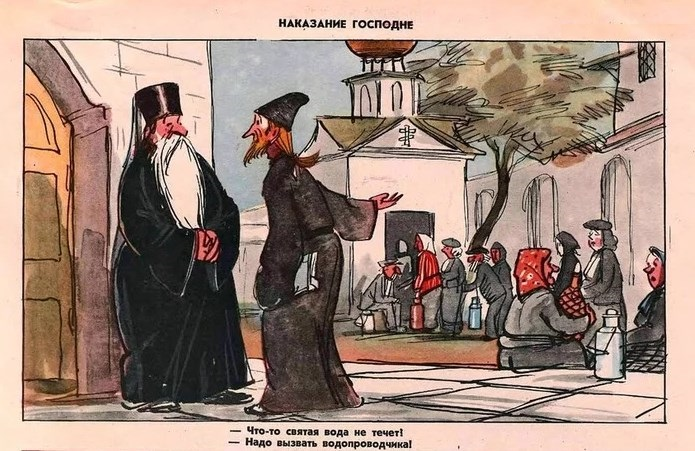
\includegraphics[width=0.8\textwidth]{img/holy-water.jpg}
\end{center}

Так ли далеко от этого ушел научный атеизм – карикатуры, которые использовались для научно-атеистической пропаганды, говорят об обратном. Например, для того, чтобы святая вода исправно поступала верующим, нужен исправно работающий водовод, а для того чтобы его отремонтировать, нужен водопроводчик.



Есть и еще одна вариация на эту тему, когда заболевший священнослужитель обращается со словами «Помоги, Господи» к аптекарю, а не собственно к Богу.

Что и чему здесь противоречит? Маловероятно, что священнослужители возьмутся оспаривать необходимость вызвать сантехника, если сломался водовод, или обратиться к врачу в случае болезни, потому как «На Бога надейся, а сам не плошай». Или вот такой опус:

\begin{fancyquotes}
    У церковного порога ждешь, поп, напрасно:\\
    Без икон и Бога мы живем прекрасно!
\end{fancyquotes}

Как говорится, слава Богу, что кто-то может решить свои проблемы своими силами и не беспокоить Всевышнего всякими мелочами:

\begin{wrapfigure}{l}{0.5\textwidth}
    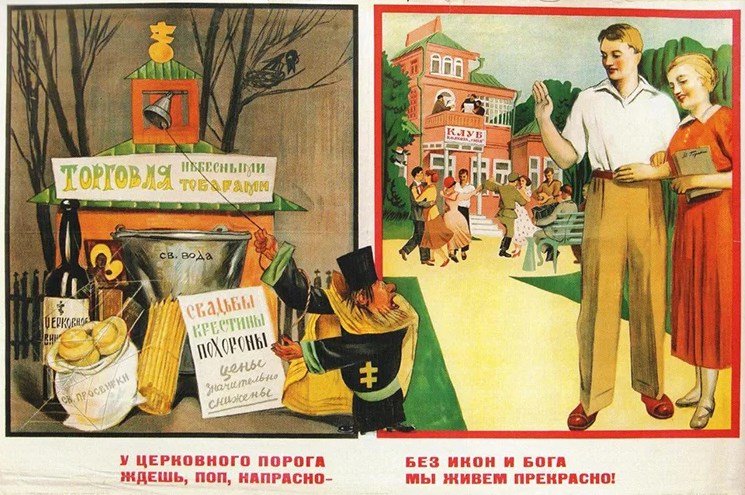
\includegraphics[width=0.5\textwidth]{img/atheism-church.jpg}
\end{wrapfigure}
Иначе может получиться, как в анекдоте, когда глубоко верующий попал и постоянно молившийся прихожанин в ад, а крепко пьющий столяр-безбожник – в рай. На вопрос верующего «Почему?» последовал вполне логичный ответ, что где это видано, чтобы табуретки бегали за столяром и «доставали» его своими проблемами.

\begin{wrapfigure}{r}{0.5\textwidth}
    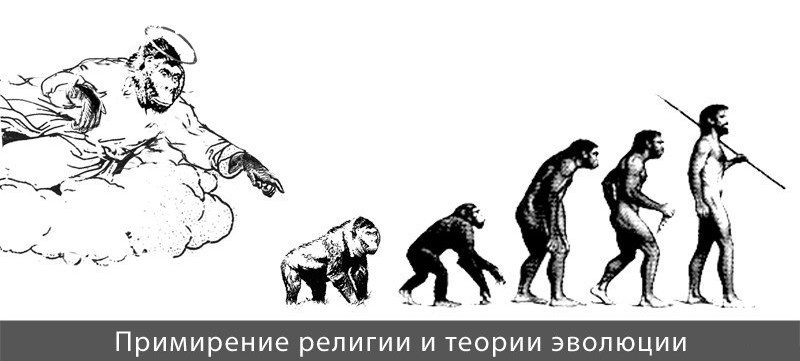
\includegraphics[width=0.5\textwidth]{img/atheism-monkey.jpg}
\end{wrapfigure}
Были, правда, и попытки «примирения» науки и религии, к примеру, по вопросу о происхождении человека. С учетом того, что живьем Бога все равно никто не видел, допущения могут быть абсолютно любые. Насколько удачные – судите сами.
Однако самой фееричной на тему научного атеизма карикатурой можно считать, пожалуй, ту, где студентка молится Богу, чтобы сдать научный атеизм:

Как говорится, «кафедра научного атеизма в шоке», но кого это волнует, когда «на кону» стипендия.

Так или иначе, и в религиозной, и в научно-атеистической пропаганде можно найти какие-то изъяны. Однако есть ученые, которые занимаются критикой научного атеизма профессионально и получают за это зарплату.\\


\textbf{Критика научного атеизма}

Сегодня в обществе существует запрос на сохранение баланса между верой и знанием, светским и религиозным, охрану личных границ от вмешательства какой-либо идеологии со стороны будь то церкви или государства. Именно этим и обусловлены циклические всплески интереса к вопросам научного атеизма.

Однако у определенной группы ученых есть большие сомнения, что научный атеизм может решить эту задачу и что в принципе в ныне существующем виде научный атеизм имеет право называться научным. Так, в статье The reasons for «scientific» atheism (Причины «научного» атеизма) можно найти витиеватую мысль насчет того, что «научный атеизм противоречит сам себе, потому что, если бы он был правдой, ему не пришлось бы трудиться, чтобы опровергнуть иллюзию» [J. Cañizares, 2012].

Стоит ли это понимать так, что если бы география была правдой, так ей бы не пришлось опровергать иллюзию многих поколений людей, что Земля плоская? А если бы правдой была химия, то ей не пришлось бы опровергать иллюзию божественного происхождения молекул и атомов, и в химических формулах и таблице Менделеева не было бы никакой необходимости? Как говорится, «не совсем понятно».

\begin{wrapfigure}{l}{0.5\textwidth}
    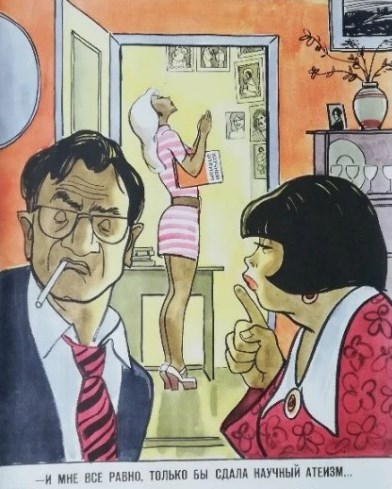
\includegraphics[width=0.48\textwidth]{img/atheism-4.jpg}
\end{wrapfigure}
Есть и более здравые мысли. Бразильский физик-теоретик Марсело Глейзер в своем интервью по поводу получения Темплтоновской премии 2019 года заявил, что «отсутствие доказательств не является доказательством отсутствия», и именно поэтому «атеизм несовместим с научным методом» [L. Billings, 2019].

Насчет того, что «отсутствие доказательств не является доказательством отсутствия», с этим нужно полностью согласиться. Однако само по себе «отсутствие доказательств отсутствия» не может автоматически считаться доказательством присутствия. В этом плане атеизм полностью следует в русле формы научного скептицизма – подхода, согласно которому, все утверждения, которые не могут быть доказаны опытным путем, должны быть подвергнуты сомнению.

Всем, кому хочется больше критики, можем порекомендовать статью «Сердце бессердечного мира: Как родился и умер советский научный атеизм» [А. Коняев, А. Артемьев, 2013]. Мы долго останавливаться на критических замечаниях не будем ввиду однотипности предлагаемых критиками аргументов и бессмысленности критики всего, что в какой-то момент времени оказалось востребованным и отвечающим запросам текущей ситуации.

В конце концов, религия – это не только идеология, которую можно принимать или не принимать, критиковать или продвигать в массы. Это красивые обряды, это душевные песнопения, это самобытная архитектура церквей. Это еще несколько праздников в наш насыщенный трудовыми буднями календарь, это возможность отдохнуть душой, отмечая вместе с близкими людьми, к примеру, Пасху.

Подготовка к этому празднеству столь же замечательна, как и само празднование: покраска яиц всей семьей, выбор узоров и красящих субстанций, эксклюзивные сюжеты и стандартные трафареты, которые нужно максимально гармонично разместить на поверхности яйца. А в день Пасхи по традиции принято устраивать «сражения», по очереди ударяя друг о друга окрашенные куриные яйца и выясняя, с какой стороны скорлупа крепче: с более округлой или с более заостренной.

Большинство людей, отмечающих Пасху и красящих куриные яйца, не читали Библию и не считают для себя обязательным посещение церкви. Стоит ли им мешать просто наслаждаться жизнью, праздниками, общением и застольем, досаждая всяческими опусами на тему научного атеизма и ненужности религии как таковой?

Думается, вряд ли, потому что у нас уже была страна, которая пыталась запрещать людям совершать церковные обряды, крестить детей и венчаться, праздновать Пасху, читать Солженицына и Довлатова, слушать «Битлз» и ДДТ. Страна называлась СССР, и ее больше нет, в то время как книги Солженицына и Довлатова читают до сих пор, «Битлз» и ДДТ как слушали, так и слушают, а Пасху как отмечали, так и будут отмечать дальше все, кто считает это нужным для себя.

Закончит так же плохо, как СССР, любая другая страна, которая будет запрещать, ограничивать и убеждать людей в том, что им не нужно многое из того, к чему они привыкли? Мы не знаем, но проверять не хотелось бы. А хотелось бы, чтобы в нашу жизнь вернулся мир, добро и взаимопонимание, причем совершенно не важно, как: через религию, науку или атеизм.

\newpage
\section{Язык и религия}

\textit{Источник: \url{https://4brain.ru/blog/jazyk-i-religija/}}
Религию можно обозначать в любых категориях – ее называют системой верований, идеологией, «опиумом», неосознанным и трансцендентальным знанием об окружающем мире. В любом виде она представляет сначала систему идей, концепций, ассоциаций и сравнений, которые могут переноситься людьми в материальную культуру.

Но, независимо от категорий, важно понимать одно: религия без слов, общего языка и системы мышления не сможет существовать больше одного поколения. Религия – это совокупность неких абстрактных смыслов, которые можно передать при помощи слов, языка.

В идеализированном понимании религия не предусматривает необходимости защищать себя от скептиков или же искать самой себе подтверждения – передачи знания и религиозных основ от поколения к поколению было бы достаточно, чтобы последователи поддерживали религию живой. Подходящей цитатой в этом случае является цитата Джалаладдин Руми (Sufi mystic Rumi): «Тишина – это язык Бога».

Но с другой стороны, исторически становится очевидным, что язык как средство сохранения религии является также и главной причиной, почему религиозные знания не могут передаваться дословно, точно, без интерпретаций, скептицизма и дискурсивности. Именно создавая новые интерпретации той или иной догмы, множество скептиков или реформистов создавали новую религию.

Таким образом, вопрос связи языка и религии – это нечто больше, чем сохранение культурной традиции. Язык и религия вызывают интерес разных мыслителей и ученых на протяжении столетий, начиная со времен Аристотеля и заканчивая сегодняшним днем (больше о последних исследованиях можно почитать в нашей статье «Язык и мышление»).

\textbf{Обозначение взаимозависимости}

С философской точки зрения, язык и религия – это два инструмента человеческого сознания, которые помогают объяснить организацию внешнего мира, создать ощущение общности. Поэтому религия и язык являются такими же формами сознания, как философия, мораль, право, искусство и наука, ибо все они преследуют единую цель – отображать мир в сознании человека.

Поскольку язык и религия – это два разных подхода к пониманию мира, для более четкого обозначения предмета дискуссии их используют вместе, как понятие «язык и религия». Это придает новое значение данным понятиям и позволяет рассматривать их наряду с другими стойкими философскими категориями, такими как «язык и общество», «язык и сознание», «язык и культура».

Но все-таки очевидным можно назвать то утверждение, что религия является более зависимой от языка. Именно при помощи языка создаются и сохраняются все религиозные образы, что делает психологические структуры языка и религии между собой тесно сплетёнными.

\textbf{Вильгельм фон Гумбольдт и «дух народа»}

Интерес к изучению истории и духа (культуры) европейских народов был заложен философом Вильгельмом фон Гумбольдтом. Вслед за философией Гегеля, который провозгласил идею «духа народа» неотъемлемой составной частью человеческого бытия, Гумбольдт развил направление сравнительной антропологии, которое интересовалось историей, бытом, фольклором и, конечно же, религией – важными составными чертами народов.

Непосредственно Гумбольдт также предположил, что язык возник как результат духовного развития народа, и это нечто большее, чем общественное сознание, – это различное видение мира. К такому заключению он пришел во время изучения языка басков, который разительно отличался от языков своей индоевропейской семьи. В своей работе «О различии строения человеческих языков и его влиянии на духовное развитие человечества» Гумбольдт описывал непосредственное влияние языка на формирование духовного сознания человека.

\textbf{Сакрализация текстов и их роль}

Наивысшей формой развития духовного сознания некой общности людей является создание собственных сакральных книг – Торы, Священного Писания, Корана, Авесты, проповедей Будды. Каждый из этих текстов стал чем-то большим, нежели просто послужил формированию народной общности, – со временем приверженцы той или иной религии не ограничивались географическими границами, могли сохранять чувство единения с единомышленниками независимо от местонахождения. Такое чувство общности оказалось даже более стойким в формировании ментального родства, чем использование одного языка, на котором тексты были написаны.

Таким образом, независимо от религии и языка, на котором передаются сакральные знания, язык и религия все равно являются важными элементами человеческого познания и объяснением мироустройства, роли человеческой жизни и жизни после смерти.

Другая важная особенность сакральных текстов состоит в том, что вокруг них формируется целая прослойка важных культурных и духовных проявлений приверженцев – особое религиозное мироощущение, традиции, обряды, религиозная мораль, религиозные институты. Все эти материальные проявления абстрактной религии делают более четкими и понятными духовную практику для многих последователей вне национальных ограничений.

\textbf{Атеистический экзистенциализм: возможна ли жизнь без Бога}

Несмотря на силу религиозного учения и его интерпретации общественного строя, другим проявлением человеческого сознания является полное или частичное отрицание божественной, мифической и духовной потребности человека в Боге в любой форме – трансцендентальной, метафизической и религиозной. Приверженцы этого философского направления – атеистического экзистенциализма (Жан-Поль Сартр, Альбер Камю, Мартин Хайдеггер и Симона де Бовуар), опровергая большинство принятых христианских канонов, не смогли выйти из религиозной перспективы мира, ибо заявили о реинкарнации как форме спасения.

\textbf{Религиозная практика сегодня}

В современном мире, транскультурные границы которого все больше и больше теряют свое значение, святость религиозного языка выглядит, как последний не тлеющий бастион. Особенно в мегаполисах или в далеких странах религия и язык часто являются самыми важными атрибутами национального и культурного единства. Молитва на родном языке сохраняет ощущение единства с культурой и историей.

В современном глобальном мире, где люди часто теряют свои корни и помнят о них из детских рассказов, изучение родного языка и молитва на нем выполняют важную практику духовного воссоединения со своими корнями. Такая тенденция наиболее популярна среди современного еврейского населения, часть которого проживает в разных странах мира. Именно язык и религия являются источниками воссоединения с прошлым. Для них иврит – это интимный способ понимания своей религии, культуры и философии в более точных понятиях. Таким образом, независимо от контекста, именно использование религиозных терминов в ежедневном лексиконе, вместе с отмечанием праздников, помогает осмысливать свое существование и историю.

С другой стороны, разнообразный исламский мир именно при помощи религиозного языка и канонов веры сохраняет свое ощущение единства – из 5 разновидностей арабского языка сиро-палестинский диалект (Levantine Arabic) – самый универсальный, и на этом диалекте написан Коран, поэтому он понятен большинству арабов.

И более того, язык религии может не только поддерживать существование национальной культуры, где бы ее последователи ни обитали, – он может создавать новые общества, объединяя разных людей. Именно такой необычный путь свойственен классическому тибетскому языку. Его первые последователи появились в Британии в 1960-х гг., где учредили монастырь и стали объединять всех желающих изучать буддизм.

\textbf{Вместо заключения}

Язык и религия как мировоззрение являются проявлением человеческого сознания, и, независимо от трансформаций, служат неотъемлемым способами познания мира человеком. Их роль заключается в более сложной функции, чем роль общественного или политического мировоззрения, ибо при помощи религии и языка человечество пытается не столько обустроить свою жизнь, сколько найти ответы на вопросы о своем существовании.
\chapter{AI}
\chapter{Иммиграция}

\textit{Россияне рассказывают, каково это — жить вдали от родины}

{
    \it В рубрике «Из жизни» каждую неделю публикуются рассказы людей, которые по разным причинам решили переехать в другие страны. Одни отправились за границу в поисках любви, другие уехали на время обучения, а третьи просто решили, что вдали от родины их ждет лучшая жизнь.
}

\textit{Источник: \url{https://lenta.ru/themes/2018/02/12/migration/}}

\section{Япония}
% --- Studied 
% --- Added to Anki

\textit{«Русские мерзнуть не могут — кожа особенная» История россиянки, перебравшейся в Японию}

Рина переехала в Японию сразу после университета и влюбилась в страну с первого взгляда. Вопреки стереотипам о не подпускающих к себе японцах она стала своей в небольшом городке, а позже — успешно ассимилировалась в мегаполисе. В рамках цикла материалов о россиянах, перебравшихся за границу, «Лента.ру» публикует ее рассказ о жизни в Токио.

После окончания университета — в тот момент я находилась в Бельгии — мне захотелось продолжить свой жизненный путь за границей. Мне казалось, что этот период времени идеален для получения новых впечатлений и погружения в другую культуру — у меня не было семьи, детей, постоянной работы.

Я подала заявления на стажировки в разные страны, включая США, Германию и Японию. Однако только в Японии стажировка оплачивалась настолько высоко, чтобы можно было поехать туда почти без накоплений. К тому же бесплатно предоставлялось корпоративное жилье.

Шесть месяцев я жила в большом центре для интернов, гостей и партнеров компании, а также командированных из других филиалов. У нас были огромная кухня, сад и даже небольшой горячий источник. По прошествии полугода мне предложили постоянный контракт без срока действия, и я сменила свой статус, получив пятилетнюю рабочую визу.

Сразу оговорюсь, что я ехала в Японию, предварительно сдав международный экзамен на знание японского языка JLPT на высший уровень N1, без этого в нашу компанию иностранцев не брали.

\newpage
\textbf{Наблюдения о Японии}

Япония — настоящий рай для эстета и гурмана. Еда здесь высочайшего качества, получить пищевое отравление практически невозможно, разве что вы сами напортачите и съедите что-то, что слишком долго пролежало в холодильнике.

Японцы помешаны на «сезонных» и «эксклюзивных» продуктах. Первое выражается в том, что регулярно выходят новые версии одного и того же товара — пудинга, мороженого, напитков, снеков — со вкусом сезонных овощей и фруктов или сезона как такового. Летом появляется куча еды со вкусом шоколада и мяты или соленой карамели, осенью — со вкусом сладкого печеного батата, тыквы, ранней весной — клубники.

Суть эксклюзивности в том, что каждая префектура в Японии славится какими-то определенными продуктами: префектура Яманаси — своим виноградом, винами, медом; Хоккайдо — морепродуктами и молочной продукцией; префектура Аомори — яблоками и яблочными пирогами; префектура Ямагата — вишней. Поэтому сладости вроде Kit Kat или косметику вроде тканевых масок для лица иногда можно найти с «эксклюзивными вкусами и ароматами». Они продаются только в конкретных префектуре или городе и основаны на самой известной продукции этого места.

\begin{fancyquotes}
    После России очень удивляет, что нет строгого контроля за продажей алкоголя. В маленьких городах много автоматов, продающих пиво и сливовое вино. В магазинах у меня лишь один раз за три года попросили удостоверение личности, чтобы проверить возраст. В основном покупатель сам жмет на кнопку на специальном экране, чтобы подтвердить, что он совершеннолетний, документы для этого не нужны. Нет запрета пить алкоголь на улице или в транспорте — в пятницу вечером в электричках очень много офисных работников, пьющих пиво
\end{fancyquotes}

Арендная плата в Токио очень высокая, но есть интересный лайфхак, как сэкономить на жилье, если вы несуеверны. Дело в том, что японцы очень не любят селиться в «нехороших квартирах», где кто-то умер или произошел какой-то инцидент. Причем это распространяется и на случаи, когда одинокий пожилой человек мирно отошел в мир иной в своей постели — ничего из ряда вон выходящего в этом нет. Так как никто не хочет заселяться в такую квартиру, риелторы снижают стоимость аренды вдвое, а иногда и втрое на первые год-два контракта аренды. После этого квартира считается «очищенной», ибо в ней жили обычные люди, и арендная плата возвращается к средней по рынку.

\textbf{О любимом времяпровождении в Японии}

Из развлечений я больше всего полюбила ездить на термальные источники. Как правило, они расположены в горах или долинах, на природе, в очень живописных местах. Источники бывают разного состава — сернистые, кислые, сероводородные, солевые — отчего они очень разные по цвету и мутности воды. Бывают и мутные, серого цвета источники, а бывают прозрачные, с водой янтарного оттенка. У всех источников разное влияние на организм, но они одинаково хорошо делают кожу блестящей и красивой, а также уменьшают боль в спине и в мышцах.



В крупных термальных комплексах огромное количество ванн с разными особенностями. Могут быть и лекарственные ванны с добавлением экстрактов растений, меда, цитрусовых, лепестков цветов. У термальных источников всегда есть гостиничные комплексы, где можно попробовать традиционный японский ужин кайсэки с множеством разнообразных миниатюрных блюд и расслабиться в комнате с татами в японском стиле, облачаясь в банный вариант юката — что-то вроде облегченной хлопковой версии кимоно.

\begin{fancyquotes}
    Я очень рекомендую этот вид отдыха всем приезжающим в Японию, но, пожалуйста, имейте в виду, что в банных комнатах и источниках можно находиться только голышом, купальники и плавки запрещены
\end{fancyquotes}

Мужчины и женщины осуществляют банные процедуры раздельно, хотя в отдаленных районах сохраняются места, где нагишом в один источник влезают все, независимо от пола. Также отдельная радость — это горячие источники для ног, неотъемлемый элемент всех термальных деревень. В них можно смыть усталость от долгой прогулки и согреться зимними днями.

\textbf{О медицине и налогообложении }

В Японии очень много типов налогов, шкала налогообложения здесь прогрессивная. Из-за чего ходит шутка, что что бы ты ни делал — работал, владел машиной или недвижимостью, приобретал их, инвестировал деньги, получал имущество или подарки, умирал — за все берут штраф, то есть налоги.

Но есть интересная система, которая называется фурусато но:зей — буквально «налоги — родному городу». Вы в течение года делаете денежные пожертвования какому-то городу, муниципалитету или селу на ваш выбор через специальную систему. В зависимости от суммы пожертвования можно выбрать подарки. Обычно это деликатесы или билеты на концерты, в музеи и парки. Но иногда встречаются интересные варианты вроде «мешка льда из Охотского моря», «дня работы на местной радиостанции в качестве ведущего» или «дня бесплатного катания на яхте по самым красивым местам префектуры».

В конце года вы идете в налоговую, предоставляете документы, что платили фурусато но:зэй. Вам делают налоговый вычет на эту сумму. Но есть ограничения по сумме максимального пожертвования, на которую идет налоговый вычет: 20 процентов резидентского налога. Допустим, если ваш годовой налог 200 тысяч йен, и вы сделали пожертвования на 40 тысяч йен, вам их возместят через вычет на 100 процентов. А если превысить эту сумму и пожертвовать 45 тысяч йен, то никто вам лишние 5 тысяч йен не вернет.

В итоге ваши пожертвования, то есть налоги, пошли любимому городу, где, возможно, мало налогоплательщиков, ваши инвестиции в него были полностью возмещены через налоговый вычет, да вы еще и подарки или продукты получили бесплатно.

Медицина в Японии не бесплатная, но даже если вы не работаете, вы сможете пользоваться государственной системой страхования здоровья. При минимальных взносах в месяц государство будет оплачивать 70 процентов от суммы вашего лечения и 70 процентов от суммы лекарств, купленных по назначению врача. Если вы работаете, взносы будут больше и тип страховки немного изменится, но все будет основано на вашем доходе — страховые отчисления тоже прогрессивны.

Вызов машины скорой помощи в Японии бесплатен, но везде висят плакаты с просьбами не вызывать скорую помощь при недомоганиях, с которыми вы способны сами дойти до больницы. В Японии есть проблемы с психологической поддержкой: консультации у психолога и немедикаментозные способы лечения совсем не развиты. От всех проблем сразу же прописывают антидепрессанты или иные лекарства, иногда с сильными побочными эффектами. Так что в случае каких-то проблем рекомендую искать психологической поддержки на родине.

\newpage
\textbf{Об общении и дружбе в Японии}

Про Японию можно часто услышать, что здесь нельзя стать своим — мол, местные всегда в вас будут видеть туриста или временного жителя, но точно человека другой культуры и других убеждений.

У меня совершенно противоположный опыт: до переезда в Токио я жила в маленьком городе сельского типа, где у людей очень тесные узы с соседями и местным сообществом в целом. Например, не раз случалось, что я приходила в посудную лавку купить чашки для чайной церемонии, а хозяин — его семья управляет этой лавкой уже не первую сотню лет — тут же звал свою жену с поля, чтобы она поприветствовала меня. В благодарность за разговор и покупки она дарила мне овощи со своей грядки — морковку, капусту, брокколи.

Еще меня звали участвовать вместе с жителями района в переноске о-микоси — маленького переносного синтоистского храма — для традиционного летнего фестиваля. Мы часто собирались с жителями района в традиционной японской рюмочной идзакая, где мне дарили праздничный торт на день рождения, утешали в сложные моменты в жизни, помогали советом. Хозяева готовили вкусности вроде сладкого рулета из яйца — конечно, все это в счет не включалось.

Я, кстати, и сейчас туда наведываюсь из Токио, меня всегда очень тепло встречают, ведь все постоянные посетители там — примерно одни и те же люди. Возможно, у тех, кто жил поначалу в больших городах, ситуация была иной, но я чувствовала очень сильную поддержку со стороны как соседей, так и сотрудников моего отдела в компании. На мой первый день рождения в Японии они мне подарили мешок сладостей и большую открытку, где каждый сотрудник от руки написал свое пожелание по-русски. Конечно, перевод был делом авторства Google-переводчика, но важно ведь внимание.

\begin{fancyquotes}
    Почти все мои друзья и приятели тут — японцы и японки. Проблем в общении я никогда не испытывала, контакты тоже легко удавалось устанавливать. Хотя, конечно, пришлось привыкнуть к тому, что подход к общению совсем другой по сравнению с Россией: предполагается, что собеседник умеет «читать между строк»
\end{fancyquotes}

Например, японец может в середине прогулки вдруг спросить: «Ты не проголодалась?» — но таким образом он будет не интересоваться вашим состоянием, а посылать сигнал: «Я проголодался, поэтому, пожалуйста, выбери какой-нибудь ресторанчик, где мы могли бы перекусить». В этом случае правильным ответом будет: «Ой, у меня как раз есть хорошее место на примете со вкусными ланчами!» или «Я не очень голодная, но как насчет перекусить вот в той лапшичной? Я могу взять какой-нибудь легкий перекус». Ответ «Нет, а что?» будет воспринят как неумение «читать» ход беседы, а собеседник в силу ментальности вряд ли скажет: «А я вот голодный, пойдем есть» — и, скорее всего, будет ходить грустный и голодный.

Так же нет культуры прямых отказов — в конце встречи вам обязательно предложат снова выпить и погулять, но исключительно из вежливости, это называется сяко:дзирэй или «социальный комплимент».

Со временем просто привыкаешь, что тот, кто в тебе заинтересован, будет более конкретен в своих приглашениях: спросит, какую кухню или фильмы любишь, поинтересуется, свободны ли следующие выходные. На приглашения с твоей стороны тоже никто напрямую отказываться не будет — несколько раз повторят, что заняты на работе, в надежде, что вы сами догадаетесь, что собеседник в вас не заинтересован. Это стандартный способ ухода от прямого конфликта, конфронтации, а также нежелание причинить собеседнику эмоциональный дискомфорт. Это не плохо и не хорошо — просто другой стиль общения.

\textbf{О работе в традиционной японской компании}

В Японии новых сотрудников без опыта, которые только-только окончили университет, не принято сразу допускать к работе. В крупных компаниях этому предшествуют обучение и практика, во время которых группу нанятых выпускников учат бизнес-этикету, инвестированию своих денег и сбережений, в том числе ради пенсии, использованию программного обеспечения, необходимого для работы, знакомят с товарами и услугами компании, дают необходимые технические или финансовые навыки. Как правило, первый рабочий день у всех начинается в апреле. Практика может длиться от месяца до полугода.

\begin{fancyquotes}
    Я работаю в промышленной отрасли, поэтому, несмотря на то, что я «белый воротничок» и работаю в сфере финансового анализа и корпоративного планирования в главном офисе в Токио, меня, как и всех, в период практики отправили на месяц работать на один из заводов компании в глухую деревню. Там я лично участвовала в создании продукции, сборке и инвентаризации, работая в ночные и дневные смены. Считается, что ты на своей шкуре должен понять, как устроена работа на всех уровнях, и не смотреть свысока из офиса на тех, кто трудится на сборочных линиях и в цехах
\end{fancyquotes}

В период практики бывшие студенты часто живут в одном большом тренировочном центре или общежитии, готовят вместе еду, устраивают вечеринки, что помогает сблизиться и стать друзьями. Все это называется словом до:ки — люди, устроившиеся в компанию в один с тобой срок. Потом, когда всех распределят по отделам финансов, продвинутого инжиниринга, новейших разработок, продаж и так далее, у вас всегда будет кто-то знакомый из до:ки в каждом из отделов, к кому вы можете неофициально обратиться и что-то спросить — это очень удобно.

В традиционных японских компаниях сотрудники делятся на несколько категорий. Сэйсяин — постоянный сотрудник с контрактом на неограниченный срок работы. Его очень сложно уволить по желанию компании — нужно доказать, что сотрудник непригоден, хотя ему дали много возможностей пройти переобучение или проявить себя в другом отделе. Кэйяку сяин — контрактник, у которого ограничен срок работы и которого можно уволить по истечении срока контракта даже без объяснения причин. Хакэн сяин — как контрактные работники, но контракт заключается не напрямую с компанией, а с рекрутинговым агентством.

В нашей компании по цвету бейджика можно понять, кто к какой категории относится. При этом сэйсяин и кэйяку сяин могут делать совершенно одинаковую работу, но премии и социальная программа поддержки у них будут абсолютно разные. Я проработала в одной и той же компании и в том, и в другом качестве, и при подписании «постоянного» контракта мой доход возрос в 1,3 раза. Мне позволили вступить в профсоюз и пользоваться какими-то дополнительными «плюшками» вроде почти бесплатной мини-гостиницы компании в деревне горячих источников. При этом мои рабочие обязанности не поменялись вообще никак.

\textbf{О России}

О России в целом знают очень мало. Меня даже пару раз спрашивали, какой у нас государственный язык, не английский ли. Молодые люди упоминали Эрмитаж, белые ночи в Петербурге, Достоевского, балет, Владивосток — его тут в поездах рекламировали как «самую близкую дверь в Европу рядом с Японией».

\begin{fancyquotes}
    Пожилые люди могут почему-то упомянуть Горбачева, но в основном их знания ограничиваются стереотипами, что все пьют водку, в том числе молодые девушки. Также, по их мнению, в России вечная зима, поэтому русские мерзнуть не могут — мол, кожа особенная
\end{fancyquotes}

В Японии вообще иностранцев — особенно европейцев и американцев — не делят по национальности или культурному бэкграунду, записывая в одну категорию «иностранцев» — гайкокудзин. Когда у нас скажут «у меня есть друг англичанин», в Японии скажут «у меня есть друг иностранец».

Японцы ужасно удивляются, когда рассказываешь им, что в России так же, как в Японии, снимают уличную обувь при входе в дом, удивляются, что мы можем есть икру. Кстати, это слово в японском заимствовано именно из русского. Часто можно услышать вопросы вроде «А вы едите вот это за границей?». Не в России, а за границей, понимаете? Приходится объяснять, что я могу отвечать только за Россию, а едят ли это в других странах мира, не знаю.

Я не хочу загадывать на будущее, потому что никогда не знаешь, что тебе принесет завтрашний день, но в Японии я нашла любимые увлечения, дорогих мне людей, в том числе молодого человека, и работу, поэтому в ближайшее время планов уезжать у меня нет. Но по родному Петербургу и культурному досугу вроде семейных походов в филармонию и на балет я очень скучаю. Надеюсь приезжать в родную страну почаще, когда пандемия пойдет на спад. О жизни в Японии и местных маленьких особенностях я рассказываю в своем Twitter-аккаунте.

\newpage
\section{Великобритания}
% --- Studied
% --- Added to Anki

\textit{«Полгода я выла от отчаяния» Рассказ россиянки о непростом переезде и жизни в Великобритании }

Наталья из России никогда не задумывалась о жизни за границей. Она училась на переводчика, была увлечена английским и практиковала его с носителями языка на сайтах языкового обмена. Все изменилось, когда она по воле судьбы познакомилась с британцем и влюбилась. В рамках цикла материалов о россиянах, перебравшихся за границу, «Лента.ру» публикует ее рассказ о непростом переезде и жизни в Великобритании.

\textbf{Роковое знакомство}

Однажды мне написал сообщение молодой парень из Англии, которого звали Райан, и предложил помочь с английским. Мы долго общались как друзья, а потом поняли, что наши отношения перетекают в нечто большее. Все закрутилось, завертелось, и в какой-то момент он купил билеты и приехал ко мне в гости. Да так в России и остался!

Изначально в наши планы не входил переезд в Великобританию. Мне нужно было доучиваться, да и работа уже была неплохая. Райан мечтал преподавать английский в чужой стране и тут же начал воплощать это в реальность. Сначала нас все устраивало.

За полгода мы проверили отношения на прочность и поняли, что идеально сходимся. Мы начали задумываться о планах на будущее. Райан не захотел навсегда оставаться в России — ему тяжело давался русский язык, и он понимал, что на родине может добиться большего. Я не хотела резких перемен, но сдалась.

\textbf{Тяжелый переезд}

Настала его очередь приглашать меня в свою страну. Я сделала гостевую визу и сорвалась к своему джентльмену. Месяцем позже, во время прогулки у Тауэрского моста, он сделал мне предложение руки и сердца. После этого мы задумались о том, как перевезти меня в Великобританию на ПМЖ.

Все оказалось гораздо тяжелее, чем мы думали. Условия визы невесты казались невыполнимыми, поэтому мы поженились в России. После свадьбы для нас наступил сложный период бюрократической волокиты, продолжавшийся целый год, так как условия визы жены были еще замороченнее.

Райану требовалось найти работу с определенным доходом и продержаться на ней как минимум полгода. Для новоиспеченного выпускника вуза это не так уж просто, но он справился. Мне нужно было пройти тест на туберкулез в специальном центре и сдать экзамен по английскому языку. Каждый раз приходилось ездить за тридевять земель.

Понадобились доказательства наших отношений. Переписки, скрины звонков, фотографии, билеты. В общем, тотальный контроль. Но без этого было не обойтись — слишком много в стране фиктивных браков ради гражданства. После всего этого бумажного ада я все-таки получила свою первую визу жены.

\textbf{Три стадии адаптации}

В Англию я влюбилась сразу. Мне нравилась британская вежливость и легкость в общении, старинная архитектура и зеленые парки, даже традиционную еду я оценила по достоинству! Именно так я и представляла Туманный Альбион, о котором столько читала в учебниках по английскому. До сих пор помню то состояние эйфории.

Мне повезло, и в первую же неделю после переезда по визе жены я вышла на работу по специальности — устроилась переводчиком. В маленьком пригороде Лондона это было большой удачей. Я до сих пор работаю в этой компании, оспаривая фразу: «Там вас никто не ждет». На работе меня, как и всех моих коллег из других стран, уважают, а мой труд ценят.

\begin{fancyquotes}
    После стадии эйфории началась вторая стадия — фрустрация. Эти фазы свойственны всем иммигрантам, как я позже узнала
\end{fancyquotes}

Несмотря на это, адаптироваться оказалось непросто. Мне было все не так. Медицина — мрак, к врачам не попасть, да и им на тебя плевать. Люди оказались открытыми только снаружи, а дружбы ни с кем не построить. Закрывается все рано, после пяти вечера город спит.

Около полугода я выла от отчаяния. Меня даже начал раздражать их акцент. Когда слышала за углом русскую речь, хотелось бежать навстречу. Но постепенно я начала ко всему привыкать: подступила к третьей стадии иммиграции — принятие.

\textbf{Минус в плюс}
Всем тяжело выходить из зоны комфорта, сейчас я это понимаю. Сначала я была слепым котенком и не знала, как тут все устроено, куда можно пойти, не понимала негласных правил общения с местными. Только спустя полгода-год я начала более-менее ориентироваться в новой среде.

Постепенно все минусы, которые меня вгоняли в депрессию, стали превращаться в плюсы. Да, многие магазины закрываются довольно рано. Но перестроиться на новый график недолго. Зато сколько разных магазинов здесь можно найти! Да и заказываю я уже все в онлайне — от продуктов и до одежды. Пара дней ожидания — и вуаля! Все, что пожелал, — у тебя на пороге.

Рестораны и кафе — отдельная тема. В Лондоне и крупных городах можно найти рестораны любой кухни. Я распробовала популярные здесь индийскую и китайскую кухни и сейчас не могу без них жить. Британские традиционные блюда в хороших пабах тоже очень даже неплохие.

\begin{fancyquotes}
    Кстати, совет, если окажетесь в Великобритании, пробуйте традиционный фиш-н-чипс именно в прибрежных городах. Там свежая вкуснейшая рыба. Да и другие морепродукты тоже, самые лучшие устрицы — у нас!
\end{fancyquotes}


\textbf{Дружба с британцами — на всю жизнь}

С самого начала я общалась только с британцами: с семьей мужа, его друзьями, девушками в студии танцев и со своими коллегами. Русских в нашем маленьком пригороде я найти не могла, а ведь даже искала первое время. Думаю, тот факт, что в моем окружении были исключительно местные, помог мне адаптироваться быстрее, хоть сначала было и невыносимо.

Со временем я начала понимать нюансы общения с британцами и перенимать их. У них принято быть очень вежливыми, например, не использовать резкие фразы, а увиливать. Наше «нет» они воспримут как грубость. У них считается нормой саркастично шутить друг над другом, и здесь уже мы, русские, можем обидеться на их подколы. Хотя все, что надо сделать, — подколоть в ответ и вместе посмеяться! Сейчас мне эти колкости кажутся безобидными и очень даже веселыми.

Что касается дружбы, то с русскими сдружиться легче. Если в России можно поговорить с незнакомцем по душам после десяти минут знакомства, то к британской душе подступиться тяжелее. Они дружелюбны, улыбчивы, но общение очень долгое время остается поверхностным. Все держится на уровне вежливых фраз: «Как дела? Сегодня такая дождливая погода. Какие планы на выходные?» Только через два года я начала теснее общаться со своими британскими знакомыми.

\begin{fancyquotes}
    Пусть получить статус друга в Англии тяжело, если вы все же сдружились — это на всю жизнь
\end{fancyquotes}

Британцы — люди толерантные и притеснять вас только из-за национальности не будут. Правда, местные не любят тех, кто отказывается адаптироваться и лезет в чужой монастырь со своим уставом. Но таких в любой стране не любят, так ведь? Если вы вежливы, приветливы и миролюбивы, вас примут как своего. Даже с жестким русским акцентом. Конечно, могут по традиции «стереотипно» подколоть про водку или вечную мерзлоту, но обижаться на это не стоит.

Толерантность британцев мне нравится. Им нет дела до жизни чужих людей, если те никому не мешают; им все равно, как ты выглядишь, во что одет, они не докапываются и редко осуждают. По моим ощущениям, здесь меньше резкости, злобы на что-то, что их не касается, да и негатива вообще.

\textbf{Партнерские отношения}

Мужчины-британцы редко оплачивают все полностью. Сразу отмечу, что во время декрета они, конечно, обеспечивают своих жен. А жена помогает мужу, если он вдруг потерял работу. В этом суть партнерских отношений, которые все популярнее в Англии. Обычно люди либо создают общий бюджет, либо делят счета.

Нам ближе вариант с общей копилкой. Мы делим и доход, и домашние обязанности. Все честно, и все счастливы. Меня с самого начала привлекал именно такой подход к совместной жизни.

Про цены, думаю, говорить особого смысла нет. Жилье, коммуналка, транспорт и услуги тут не самые дешевые. Но это восполняется высокими зарплатами. Цены на еду примерно на том же уровне, что и в России, а одежда и другие мелочи стоят дешевле. В целом у меня тут остается намного больше денег от зарплаты, чем оставалось, когда я работала на родине на той же должности.

А вот о местной медицине иммигранты спорят постоянно. Начнем с того, что здесь не залечивают. Если у вас обычная простуда, то вам просто скажут идти домой и пить горячий чай. В таком подходе есть свои плюсы. Если у вас что-то серьезное, то все будет зависеть от доктора.

Мне попадались и те, кто на явную проблему махал рукой, и те, кто из кожи вон лез, чтобы понять, что со мной произошло. Но так было и в России — тоже по-разному. Поэтому тут все довольно неоднозначно.

\textbf{О путешествиях, традициях и самобытности местных жителей}

Один из важнейших плюсов жизни в этой стране для меня — возможность свободно путешествовать. В любую страну Европы можно долететь дешево, быстро и без виз (если уже есть британский паспорт). По самой Великобритании путешествовать тоже удовольствие — местные сохранили огромное количество замков, дворцов, поместий, да и их деревенские домики стоят веками и не меняют внешний вид. Англичане ценят и хранят свои традиции.

Британцы любят собираться на традиционный полуденный чай, говорить о королевской семье, которая тоже стоит во главе страны исключительно ради поддержания традиции. Их любимое место — старинные пабы, где по сей день пьют горький эль, закусывая традиционными свиными шкварками. Многим в Великобритании нравится эта самобытность.

Несколько месяцев назад я получила британское гражданство и паспорт. Это был тяжелый процесс — нужно было пройти через две визы жены, получение ПМЖ и натурализацию. Каждый процесс сопровождался длиннющим списком условий и ценником, от которого волосы встают дыбом.

На весь иммиграционный процесс мы потратили около десяти тысяч фунтов стерлингов (почти миллион рублей). Ставки на иммиграционные сборы в этой стране — одни из самых высоких. Но для нас все это, наконец, позади.

\textbf{Великобритания — новый дом}

После семи лет в Великобритании я могу уверенно сказать, что полностью адаптировалась и люблю это место. Тут я уже четверть жизни и смело называю эту страну своим домом. Конечно, как и везде, здесь есть недостатки. Но я акцентирую внимание только на положительных вещах, которых тоже много. Да и вообще, я всегда стараюсь идти по жизни с поднятой головой!

Скучаю ли по России? Наверное, уже нет. Я слишком привыкла к своему быту здесь. В Англии моя семья, мой дом, мои друзья, моя работа и мое увлечение. В России остались родные, и по ним я скучаю, но стараюсь их навещать.

Мне просто некогда грустить: я работаю в офисе, преподаю английский и русский как иностранный, занимаюсь танцами, учу испанский в разговорных клубах, хожу с подругами на полуденный чай и стараюсь каждые выходные проводить в новом английском городке. Путешествия — наше с Райаном основное хобби. Я прошла все психологические фазы иммиграции и, наконец, счастлива как никогда!

\newpage
\section{Арабские Эмираты}
% --- Studied
% --- Added to Anki

\textit{«Это ли не сказка?» История россиянки, которая лишилась работы и переехала в Арабские Эмираты}

\textit{Александра из Москвы не верила, что когда-нибудь побывает в Дубае, и уж тем более не мечтала о переезде туда. Однако пандемия все изменила: они с мужем лишились работы дома, и им пришлось перебраться в Объединенные Арабские Эмираты. В рамках цикла материалов о россиянах за границей «Лента.ру» публикует рассказ Александры о жизни в ОАЭ.}

Еще лет шесть назад я смотрела фотографии одноклассниц в Instagram из Дубая и думала: «Вау, как красиво и богато». Тогда я была уверена, что не смогу тут побывать хотя бы раз. Кто бы мог подумать, что судьба сложится так, что спустя пять лет мы с мужем и ребенком сюда переедем?

\textbf{Быстрый переезд}

Мы с мужем жили и работали в Москве, у нас обоих был бизнес: у него массажные кабинеты, у меня студия красоты. Потом я забеременела, и случилась пандемия. Мне кажется, в те времена паника накрыла всех. Работать мы не могли, все закрыли.

И тут мужа приглашают на работу в Дубай. Он улетел на месяц один. С работой все сложилось, и встал вопрос о переезде. Когда он вернулся в Москву, я родила. Мы быстро сделали загранпаспорт дочке, и муж полетел обратно. За месяц он должен был найти для нас жилье и арендовать машину. А передо мной стояла непростая задача: перелет с двухмесячным ребенком в неизвестную страну. Благо моя мама согласилась лететь со мной и помогала мне.

Прилетев сюда из холодной осенней России, я, конечно, была в шоке. Эти огромные стеклянные высотки, везде пальмы. Больше всего в моей голове не укладывалось, что этой стране всего 49 лет.

Первое жилье мы сняли в районе Дубай Марина. Довольно туристическое и популярное место, там все еще и «на спорте». В каждом доме есть свой бассейн, свой спортзал, до пляжа рукой подать. Это ли не сказка?

\begin{fancyquotes}
    К сожалению, за год жизни здесь большим количеством друзей мне обзавестись не удалось. И так как муж все время на работе, а я дома с ребенком, я чувствую себя немного одиноко

    \begin{flushright}
        Александра
    \end{flushright}
\end{fancyquotes}

\textbf{Быт и отдых местных жителей}

Дубай — город, куда все приезжают работать, зарабатывать и жить для себя. В выходные дни, здесь это пятница и суббота, все гуляют по торговым центрам, барам, ночным клубам. Арабы в выходные любят выезжать на пляж на целый день большими семьями: бабушки, дедушки, мамы, папы, дети. Они возят с собой ковры, столики, складные диванчики, все это раскладывают на песке, накрывают стол и устраивают этакий пикник у воды. Также они любят парки аттракционов, типа тематического парка в стиле Голливуда Motiongate или парка с 90 павильонами, посвященными разным странам мира, Global Village.

Местные жители очень активно пользуются услугами клининга, а еще больше — услугами нянь. Такого понятия как «декретный отпуск» здесь нет. После рождения ребенка мама, если она работает, должна выйти на работу через три месяца. Поэтому здесь нанимают нянь, либо отдают детей в аналог яслей, Nursery, для совсем маленьких деток. На детских площадках 90 процентов детей гуляют с нянями.

Что-то вроде «материнского капитала» выплачивается только местным гражданам и потом им же платится ежемесячное пособие на детей до 18 лет, но там немного, около 150 долларов (11 тысяч рублей). Если иностранная гражданка родила здесь, то гражданство ребенку все равно никто не даст. Более того, если в семье «араб — иностранная гражданка» рождается ребенок, только отец решает, какое гражданство он получит — арабских эмиратов или же по матери.

Роды здесь платные, кесарево сечение можно выбрать не только по медицинским показаниям, но и просто по желанию. 95 процентов местных женщин именно этот способ родоразрешения и выбирают, чтобы «не напрягаться».

\textbf{Медицина, магазины, аренда жилья и городской транспорт}

Мы с дочкой проживаем по туристической визе, каждые три месяца продлеваем ее за деньги. Поэтому и страховка у нас — туристическая. С таким типом страховки больницы связываться особо не хотят, поэтому болеть здесь очень накладно. Однажды нам пришлось обратиться к педиатру, и один прием нам обошелся в 450 дирхам (около девяти тысяч рублей).


Здесь очень любят бюрократию. Например, чтобы арендовать квартиру, приобрести сим-карту, а также открыть счет в банке — у вас должно быть личное удостоверение Emirates ID. Когда арендуешь квартиру, оформляется EJARI — это официальный государственный документ, свидетельствующий о том, что ты теперь живешь в квартире, и все счета будут приходить на твое имя.

Здесь нельзя, как в России — отдал деньги арендодателю и живешь. Когда EJARI готов, заключается отдельный договор с каждой службой, предоставляющей определенную коммунальную услугу: электричество, воду, газ и систему кондиционирования. Что интересно, в России при строительстве домов устанавливаются отопительные системы, а здесь сплит-системы — состоящие из двух блоков кондиционеры, которые служат как для охлаждения воздуха, так и для нагрева. Совсем холодной воды в домах тоже нет.

Еще один момент, который меня после России просто поверг в ступор, — интернет. Точнее, его дороговизна и недоступность.

\begin{fancyquotes}
    Обычный Wi-Fi дома обойдется вам в 400 дирхам (восемь тысяч рублей)! Да-да, именно в восемь тысяч рублей, и это еще по-божески. А за сим-карту с интернетом вы будете платить около 300-500 дирхам (от шести до десяти тысяч рублей). Поэтому, когда вы будете думать, что тысяча рублей за телефон каждый месяц — это дорого, вспомните о моих словах

    \begin{flushright}
        Александра
    \end{flushright}
\end{fancyquotes}

В городе есть общественный транспорт: метро, автобусы, трамваи. Трамваи ходят только на очень маленькие расстояния — буквально пару улиц и есть всего в паре районов. В метро несколько веток, расстояния между станциями довольно большие. Кстати, поезда в метро и трамваи ездят без водителей, поэтому очень интересно прокатиться в первом вагоне. Автобусы ездят по всему городу по расписанию. Но расстояния между остановками тоже довольно большие, поэтому дорога своим ходом может занять немало времени.

Такси здесь дорогое: поездка в одну сторону (около 20 минут езды) будет стоить вам около 60-70 дирхам (от 1,2 до 1,4 тысячи рублей). Но надо отдать должное, все таксисты работают официально, везде есть счетчики, можно оплатить картой и даже есть Wi-Fi. Водители всегда в рубашках и помогают открыть и закрыть двери, вытащить коляску и сумки.

В продуктовых магазинах тоже все очень клиентоориентировано. Овощи и фрукты всегда взвешивают сотрудники. В мясном отделе вам бесплатно разделают выбранный кусок говядины. Интересный факт: здесь вы с трудом найдете свинину, но практически во всех мясных лавках встретите мясо верблюда. На кассе специальный сотрудник соберет вам продукты в пакеты. Кстати, пакетов очень много, раскладывают чуть ли не каждую коробочку в отдельный пакетик. А еще пакеты здесь бесплатные.

\begin{fancyquotes}
    Алкоголь продается только в специальных магазинах, их немного, но они раскиданы по всему городу. В основном они находятся на парковках у торговых центров. Никаких вывесок, реклам или указателей на эти магазины вы не увидите. Поэтому найти их крайне сложно, только по чьей-то наводке. И цены на алкоголь здесь в два раза выше, чем в Москве

    \begin{flushright}
        Александра
    \end{flushright}
\end{fancyquotes}

Местное население алкоголь покупать практически не может: только местные мужчины со специальной лицензией, женщинам же это запрещено совсем. Туристам продают спиртное только по паспорту и лицензии (30-дневной или полученной от местного работодателя), при этом надо быть старше 21 года и следовать определенным правилам: нельзя пить в общественных местах, кроме баров и ресторанов, появляться на публике в нетрезвом виде и водить в таком состоянии автомобиль.

\textbf{Отношение к русским и детям}

Когда говоришь местным жителям, что ты из России, сразу все отвечают: «О, Путин!» Потом некоторые начинают рассказывать, что тоже были в России. Но для них Россия — это и Россия, и Казахстан, и Узбекистан, и Грузия. Вообще, все очень позитивно и дружелюбно относятся к русским, негатива в свой адрес мы не встречали.

А как здесь любят детей! Из-за того что все карьеристы, дети — это уже роскошь. Поэтому детей обожают. Каждый машет рукой, улыбается и даже пытается потрогать мою дочь, когда мы куда-то идем. А некоторые пакистанцы и индийцы просили сфотографироваться с ней или подержать за руку. Кто-то просто самовольно фотографирует ее. К этому мне было тяжело привыкнуть.

Про Эмираты ходит много слухов и существует много разных мнений. К примеру, что здесь при рождении каждому гражданину государство открывает счет, на котором до совершеннолетия копятся деньги. Это не так. Домыслы, что ОАЭ живут только за счет нефти — тоже неправда! Изначально страна разбогатела из-за добычи и продажи жемчуга. Здесь до сих пор почитаются искатели жемчуга (например, в Дубай Молл им посвящен целый фонтан).

Также я была удивлена, что Дубай принадлежит по сути не только арабам, но и индусам. Можно сказать, что число представителей обеих национальностей, проживающих в городе, примерно одинаковое. Очень много индийских продуктов, магазинов, вообще рынок на них очень ориентирован.

\textbf{Мусульманские традиции}

Моя подруга, когда приехала ко мне, боялась жевать жвачку и ходить в шортах, якобы здесь это запрещено. Но нет, Дубай — туристический город и максимально европеизированный. Здесь не все так строго, как нам рассказывают по телевизору.

Да, совсем наглеть не стоит и уважать традиции и веру местных нужно. Но Дубай и Арабские Эмираты в целом идут в ногу со временем, а в чем-то даже опережают другие страны.

\begin{fancyquotes}
    Наиболее устаревшие законы постепенно отменяются: не так давно мусульманским женщинам разрешили водить машину, а еще разрешили совместно жить неженатым парам — раньше сожительство преследовалось по закону

    \begin{flushright}
        Александра
    \end{flushright}
\end{fancyquotes}

Однако запреты все равно есть. Например, в государственные учреждения нельзя входить женщинам с открытыми плечами и в юбке или шортах выше колена. Запрещено открыто проявлять чувства на улице: нельзя много целоваться и слишком открыто трогать друг друга.

Запрещено фотографировать других людей без их согласия. К примеру, однажды я сфотографировала очередь в молле, и охранник сразу подошел, вежливо попросил удалить фотографию и проследил, чтобы я точно это сделала. Нельзя трогать и подходить к людям, которые молятся. Не все успевают оказаться в мечети во время молитвы, некоторые молятся на улицах, площадях и так далее. Еще из-за пандемии сейчас везде запрещено танцевать.

В целом нам здесь нравится. Я даже завела блог в Instagram, в котором рассказываю про жизнь в Дубае. Это чистый и светлый город с огромными возможностями работать и зарабатывать. Скучаю я здесь только по родственникам. Но у меня такие классные друзья и семья, что они уже несколько раз смогли прилететь к нам в гости!

Да, здесь есть свои особенности. Да, нужно время, чтобы обзавестись новыми знакомствами и влиться в эту атмосферу. Но мы молоды, полны жизни и энергии. Когда нам пробовать, если не сейчас?


\newpage
\section{США и Канада}
% --- Studied on 23 and 25 Feb 2023
% --- Added to Anki

\textit{«Стыдно за Родину не было» История россиянина, который уехал в Америку за мечтой, вернулся спустя 25 лет и не пожалел}


\textit{Владимир Томшин четверть века прожил в США и Канаде ради близости к легендам тяжелого рока. Сложно ли было на такое решиться, авантюра это или полезный опыт, и почему спустя 25 лет музыкант принял решение вернуться в Россию? В рамках цикла материалов о россиянах за границей «Лента.ру» публикует рассказ Владимира о жизни в Северной Америке.}

\textbf{В погоне за мечтой}
В начале 90-х я был увлечен тяжелым роком. Играл на гитаре в нескольких группах, которые придерживались этого стиля. На тот момент нашими кумирами были Metallica, Megadeth, Pantera, Slayer. А их родина, как известно, Северная Америка. Поэтому у меня возникло стремление поехать туда, чтобы реализовать свои музыкальные способности и умения. Сказано — сделано. Долго ждать не пришлось, визу в США я получил без особого труда.

\begin{fancyquotes}
    На тот момент у меня, казалось бы, было все, что нужно для счастья: группа, в которой я играл, любимая девушка, работа, семья и интересное хобби. Однако желание стать рок-звездой, «играть музыку» на Западе взяли свое
\end{fancyquotes}

Оставив все, я рванул через Атлантику, как мне казалось, на разведку. Думал, что посмотрю, поиграю и вернусь. Однако судьба распорядилась иначе. После шести месяцев жизни в США я узнал, что моя группа распалась, а девушка не дождалась. А вот в Америке мне очень понравилось, и я решил остаться.


\textbf{Неидеальная Америка}

Америку нам всегда рисовали сказочной страной с небоскребами, красивыми мотоциклами и машинами, ровными дорогами и денежными купюрами — всемогущими долларами. Я был готов удивляться и погружаться в незнакомый образ жизни. Шаг за шагом познавал новый для меня континент, людей, их стиль жизни. Отчасти даже пытался подражать им.

Некоторые стереотипы оказались правдой. Улыбчивые люди, полки, полные красивых вещей, супермаркеты, похожие на музеи, добродушные полицейские, машина или две в каждой семье, дома с бассейнами, наличие оружия у населения — вот она красивая жизнь и успех. Для человека, приехавшего из России 90-х, это было похоже на сказку.

\begin{fancyquotes}
    Однако и разочарования не заставили себя долго ждать. Контраст богатства и нищеты в Америке разительный. Пожив немного в этой сказке, ты начинаешь понимать, что попал в трудовой лагерь с усиленным питанием
\end{fancyquotes}

Чтобы держаться на поверхности, надо работать денно и нощно. Большинство моих знакомых имели по две, а то и по три работы. Тебе некогда наслаждаться жизнью, ты постоянно работаешь (не считая 14 дней годового отпуска), потому что надо платить по счетам.

Главным для меня как музыканта было то, что я приехал в Америку играть музыку. Но внезапно понял, что мне некогда этим заниматься, ведь надо беспрестанно работать. Музыка может тебя содержать только в том случае, если ты уже достаточно известен, а это достигается годами. Плюс колоссальная конкуренция. Ведь в каждом доме помимо оружия и машин есть еще и гитара. Музыкантов разного уровня в Америке больше, чем можно себе представить.

\textbf{Новый \explain{поворот}{turn (n.)}}

Недолго пожив в США, я уехал в Канаду. Почему? Да потому что в США считается, что в Канаде жизнь легче. Социальное обеспечение в этой стране действительно лучше, есть почти бесплатная медицина. Но реальность, как обычно, заметно отличалась от мифа.

Первое время, до получения вида на жительство, было нелегко. На высокооплачиваемую работу рассчитывать не стоило. Преодолевать языковой барьер приходилось при каждом разговоре. Спасало то, что Монреаль, где я жил, находится во франкоязычной провинции Квебек. Там английский — второй язык по значимости, и местные жители знают его похуже, чем в других провинциях. Это дало время подтянуть языковые навыки.

\begin{fancyquotes}
    Канада и США — страны иммигрантов. Крупные города разбиты на районы по национальному признаку: французский, итальянский, еврейский, греческий, арабский…
\end{fancyquotes}

Монреаль — не исключение, хотя есть и районы, где совершенно не имеет значения, какого цвета у тебя кожа или какого ты вероисповедания. Большинство граждан ведут себя достаточно мирно. Открытую агрессию я встречал всего пару раз за 16 лет жизни — и то не от местных.


\textbf{Ностальгия все же не миф}

Я много слышал и читал о ностальгии, но не думал, что испытаю это сам. В свободное время я стал больше общаться с нашими иммигрантами. Местные жители — отличные ребята, но друзьями стать не получилось.

Есть мнение, что стать «своим» в другой стране можно, только если попал туда до 20 лет и учился в местной школе и университете. Тогда есть шанс впитать менталитет и завести друзей. А я приехал туда в 23 года и переучиваться не стал. Зачем, если у меня за плечами Уральский государственный технический университет? Я до сих пор считаю, что советское образование было лучшим в мире.

Познакомился с местными музыкантами и вспомнил, что приехал сюда играть музыку. А на нее времени не хватает, потому что жизнь превратилась в рутину.

\begin{fancyquotes}
    Некогда удивительные вещи превратились в обыденность. Деньги оказались просто деньгами, а не манной небесной. Их, как и на Родине, надо зарабатывать
\end{fancyquotes}

А какие-то вещи стали даже раздражать, например, вечный ремонт дорог. Из-за него Монреаль с каждым годом стал все больше походить на полосу препятствий. Невольно начинаешь проводить параллели между нашими мирами и культурами. Со временем стало намного приятнее выражать свои мысли на великом и могучем русском языке, чем пытаться объяснять что-то на английском или французском.

\textbf{Хлеб и зрелища}\footnote{Хлеб и зрелища: Bread and spectacles}

В обычных маркетах еда безвкусная. Я ее называю «пластиковой», настоящий вкус почти отсутствует. Молоко пить невозможно, зелень напоминает обычную траву, мясо хоть и свежее, но неестественно пресное, хлеб похож на вату. Перед возвращением в Россию, несколько лет я старался покупать продукты в русских, китайских и арабских магазинах, а также у местных фермеров на единственном на полуторамиллионный город рынке.

В русских магазинах можно купить такие деликатесы, как соленые огурчики и селедку, пельмени и хлеб домашней выпечки, побаловать себя салатом оливье или селедкой под шубой. А еще приобрести красную икру. Рыбу ловят в местных реках, но канадцы не понимают вкус икры. Сетевые маркеты ее не закупают, ведь она не пользуется широким спросом.

Рестораны не блещут разнообразием меню. Основное блюдо — стейк с овощами или итальянской пастой. Очень редко в заведениях можно встретить супы. Три-четыре салата — уже богатый выбор. Исключения составляют русские рестораны. Там выбор в два раза больше по определению. Естественно, есть и традиционные блюда, такие как борщ, рассольник, пельмени или курица с грибами. Хотя, вернувшись в Москву, я понял, что еда — не такой уж крутой показатель.

Развлечения в Канаде разные — на любой вкус. Одна поездка на Ниагарский водопад дорогого стоит. Это увлекательное и незабываемое путешествие. Кроме посещения смотровой площадки есть возможность подойти на корабле к падающей воде и оказаться в пелене брызг. Еще можно подняться на воздушном шаре или облететь водопад на вертолете, а также посмотреть на это чудо природы изнутри, из-за стены.

Есть яхт-клубы, лыжные спуски, оздоровительные комплексы с саунами и бассейнами и много чего еще. Мы частенько снимали шале в лесу у одного из озер, коих в Стране кленового листа великое множество. Там мы вспоминали свое пионерское прошлое, жгли костры, пели песни под гитару, ходили на каноэ, рыбачили.

\begin{fancyquotes}
    Есть и другого рода развлечения: казино, стрип-клубы, дискотеки. На одной из них я подрабатывал вышибалой, почти как в фильме «Дом у дороги»
\end{fancyquotes}

Летом проводится множество фестивалей. Для представителей ЛГБТ есть целый квартал.

Метро и автобусы ходят исправно, как часы. Правда, порой их работники бастуют. Я был удивлен, узнав о специальных ночных маршрутах. Весьма удобно, если возвращаешься домой поздно и без машины, потому что такси — очень дорогой транспорт. Только посадка в машину стоит 3,5 доллара, а минимальная поездка (два километра) обойдется в 20 баксов.

Что касается жилья, то в Канаде вы либо покупаете недвижимость в ипотеку, либо снимаете. Второе — достаточно удобно, все условия прописываются в договоре и четко соблюдаются арендодателем. Покупать жилье в большом городе нерентабельно. Особенно, если живешь один или не любишь сидеть на одном месте. Так, мне удалось пожить и в пентхаусе, и в доме на берегу озера. За квартиру обычно платят отдельно от коммунальных услуг, а за электричество выставляется специальный счет. Сумма зависит от отопления и подачи горячей воды.

Несоизмеримо дорогая и ненадежная мобильная связь. Только выехал за пределы города — сразу все звонки, в том числе и входящие, оплачиваются по повышенному тарифу. Несмотря на высокие зарплаты, практически все стоит гораздо дороже относительно российских цен. Я пришел к выводу, что у нас цены вполне соответствуют качеству, что не всегда можно сказать о Канаде.

Мне приходилось обращаться к канадской медицине несколько раз, в том числе к дантистам (это отдельная статья расходов). В Канаде медицина существует на налоги граждан. Меня обслужили вполне достойно, я не жалуюсь. Хотя от друзей слышал неприятные истории про долгое ожидание помощи и не лучшее лечение. Фармацевтический бизнес очень развит: людей пичкают всеми возможными и невозможными лекарствами. Сначала выписывают таблетки от болезни (они тоже недешевые), а потом — лекарства от побочных эффектов, вызванных первыми. Многие так и живут.

\textbf{Общение с местными}

Местные жители — вполне нормальные люди, со своими плюсами и минусами. Никто не относился ко мне отрицательно или враждебно. Могу сказать, что в Канаде более мирное население, чем в США. У тех — извечный расовый вопрос всегда стоял ребром. Ко мне тоже относились с подозрением, пока не узнавали, что я русский. Тогда напряжение спадало само собой. В Квебеке франкофоны более терпимы к иммигрантам, чем к англоговорящим канадцам.

Естественно, было много вопросов о нашей стране. Удивление вызывало то, что в России не везде холодно, а погода в Москве очень схожа с монреальской. Встречались и те, кто уже ездил в нашу страну туристом и достаточно лестно о ней высказывался. По крайней мере, стыдно за Родину не было.

\begin{fancyquotes}
    Их главный стереотип о нас, я уверен, создала телепропаганда. То, что мы угрюмые и злые люди, поголовно состоим в русской мафии, а наши девушки самые красивые
\end{fancyquotes}

Все эти мифы были развенчаны после общения с нашими ребятами и со мной лично. Кроме последнего — тут не поспоришь. Наши девушки были и остаются на пьедестале красоты.

Трудно сказать, какие мои стереотипы о канадцах были разрушены. Я прожил там достаточно долго. Часть канадского менталитета укоренилась и во мне. Уже здесь, в России, мои друзья и знакомые отмечали разницу в мышлении и поведении. Некоторые даже акцент улавливают, хотя это уже происходит реже, чем раньше. Иногда бывает трудно подобрать русские слова, в то время как их английские аналоги вертятся на языке.

\textbf{Новые цели и планы}

В ближайших планах — записать четвертый студийный альбом «Томшин Бэнд» и акустический сборник, снять еще один клип и проехать по всей России с гастрольным туром. Творческих идей очень много. Главная цель на новом витке жизненной спирали — донести до слушателя мои песни. Я ведь и в Канаду поехал благодаря любви к музыке. А на Родину вернулся, когда понял, что мой слушатель именно здесь.

Канада — замечательная страна, но я артист, которому нужна своя публика. Большинство моих песен на русском языке. Важно, когда в зале дословно понимают то, что ты хочешь рассказать (в моем случае — спеть). На английском песни тоже есть, но он для меня не так органичен.

\begin{fancyquotes}
    В Канаде у меня осталось немало друзей. Могу сказать, что скучаю по ним и нашему общению. Так что ностальгия у меня теперь двойная
\end{fancyquotes}

Хотелось бы также съездить в Северную Америку с гастролями, показать, насколько изменилось и «выросло» мое творчество. Конечно, видео с выступлений доступны в интернете, но живой концерт — это особая энергетика.

В любом случае я благодарен судьбе за возможность получить бесценный опыт долгосрочного проживания в Канаде. Но рад и тому, что осознание настоящего предназначения вернуло меня на Родину.


\newpage
\section{Болгария}
% --- Studied on 25 Feb 2023
% --- Added to Anki

\textit{«Здесь люди уважают себя и свой труд» История россиянки, которая переехала с тремя детьми на родину мужа — в Болгарию}

\textit{Два года назад Наталья перебралась из России в Болгарию — на родину своего мужа. За это время она обжилась в стране, где до того бывала лишь в качестве туристки, и увидела ее с новой стороны. В рамках цикла материалов о россиянах, перебравшихся за границу, «Лента.ру» публикует ее историю.}

Мой муж — наполовину болгарин, и поскольку его родители работали в разных странах, он в разное время жил в Москве, хорватском Загребе и болгарской Софии. Он учился в Софийском университете, затем перевелся в Московский университет, где мы с ним и познакомились. Мы поженились и жили в Москве. У нас родились три ребенка с маленькой разницей в возрасте, мы работали в хороших местах и каждое лето ездили в отпуск на море в Болгарию к родственникам мужа в небольшой город Ямбол.

Муж всегда хотел вернуться обратно в Софию, город своей молодости, где ему было комфортнее, чем в Москве. Он жил в столице во многом ради меня, потому что я считала, что в России мы добьемся большего и лучше обеспечим детей. К тому же мы не знали, сможем ли устроиться в Болгарии. В маленьком приморском Созополе, где мы были летом, работы вообще не было, и родственникам мужа из Ямбола приходилось работать в Германии.

Несколько лет назад мы съездили в отпуск не на море, как всегда, а в горы и в Софию, поговорили со школьными и университетскими друзьями моего мужа, которые там учатся и работают, и поняли, что мы тоже можем попробовать переехать в Болгарию. Тем более, что старший ребенок подрос, пришло время отдавать его в первый класс и выбирать между российской и болгарской системами образования.

Я знала, как мягко и терпеливо болгары относятся к детям, и хотела выбрать болгарское образование. Тем более, что умному ребенку в этой стране легко поступить в хороший университет. Кроме того, мы с мужем решили, что в Болгарии безопаснее, чем в России. В этой стране детей отпускают в школу без взрослых и разрешают самим ездить на общественном транспорте. В итоге мы решили переехать в Болгарию.

Путь получения ПМЖ и потом гражданства в Болгарии довольно долог: сначала нужно пять лет жить с видом на жительство и продлевать его раз в год. Нужно готовить много документов. Муж должен нотариально заверить текст, согласно которому он готов содержать жену, а его брак не фиктивен. Собственник жилья — что готов его сдавать. Еще нужен договор с работы или счет в банке с 12 минимальными окладами и страховка. Подготовить их не так уж сложно, проблема в том, что у сотрудников миграционных служб разные представления о том, что именно нужно. Они могут просить добавить то один, то другой документ, хотя сами видели наших детей и точно знают, что брак не фиктивный.

Нас несколько раз приглашали на собеседование, где мы заполняли большие анкеты о качествах супруга. Это может немного затянуть получение вида на жительство, который в первый раз дается на основе визы D. Получать эту визу надо в московских консульствах, и это совсем не сложно. Главное, чтобы был работающий болгарский телефонный номер и номер собственника жилья, в котором будете жить, потому что сотрудник миграционной службы может на него позвонить.

Хотя Болгария — это совсем не Франция и не Италия, куда можно мечтать поехать в романтический отпуск, я всегда любила эту страну. Это была первая зарубежная страна, в которой я побывала. Тогда мне было 14, мы с сестрой ездили отдыхать в лагерь в Золотых Песках. Мы жили в обшарпанном советском пансионате со сломанными замками на дверях, куда надо было подниматься от пляжа по длинной вертикальной лестнице. Но сам курорт был очень ухоженным, а в соседнем городе Балчике были такие милые болгарские домики с черепичными крышами...

\begin{fancyquotes}
    Мы с сестрой, две маленькие девочки, могли спокойно сами пойти в кафе и поесть там. Все это давало какую-то радость жизни и свободу, которую я до сих пор ощущаю в этой стране
\end{fancyquotes}

Возможно, поэтому, когда мы только переехали, я и ощущала эту эйфорию, хотя объективно нам было непросто. За три дня на машине проехать пять стран с тремя маленькими детьми, при этом вовремя подключаясь к вайфаю в гостинице, чтобы успеть на наши с мужем удаленные работы. Сперва остановились в маленьком горном курорте Сандански, где муж мечтал немного пожить после огромной, по его меркам, Москвы. Затем поехали в провинциальный Ямбол, где жили около цыганского квартала и работали удаленно практически каждый день.

Приходилось постоянно преодолевать какие-то препятствия: разбитую фару Chevrolet заказывали аж из Москвы, миграционная служба требовала новые и новые документы, потом мы переезжали из Ямбола в Софию, и нужно было искать школу и сад для детей. Но это казалось чем-то естественным, необходимым и неизбежным при эмиграции.


Изначально мы приехали, имея две удаленные работы. В Софии муж сразу же нашел хорошую по здешним меркам работу. Но у него очень хороший уровень английского, русского и болгарского, к тому же в Москве он работал руководителем отдела. Я примерно через год устроилась на работу по рекомендации мужа, но через полгода меня уволили из-за не поданных вовремя документов для продления договора. Честно говоря, из-за слабого знания английского мои показатели в работе были настолько низкими, что рано или поздно меня все равно бы выгнали.

Оставшись без работы, я пошла на бесплатные интенсивные курсы болгарского языка, а потом стала учить язык уже за деньги, так как найти бесплатные курсы моего уровня не так просто. В итоге теперь моего знания болгарского языка почти хватает для получения гражданства. А гражданство даст мне массу преимуществ. Например, можно будет ездить в Европу без визы и, если понадобится, работать там. Кроме того, я получу право на бесплатную медицину в Болгарии.

Параллельно я продолжала искать работу и сходила на собеседования в несколько крупных международных кол-центров. Хотя во многих мне удалось пройти несколько ступеней — интервью с эйчаром по телефону и лично, тесты по русскому и английскому языкам, включая технические, — выбирали не меня, а более сильных кандидатов с продвинутым английским и с опытом работы в этой сфере. В результате я по-прежнему брала фрилансы от знакомых из России и через бывшего коллегу нашла подработку в качестве риелтора в крупной болгарской компании «Имотека». Суть моей работы в качестве «внешнего брокера» очень проста: искать новых клиентов, которые хотят купить или продать квартиру, и знакомить их с представителем компании в нужном регионе.

Местные жители относились и относятся ко мне исходя из моей роли в их жизни. Когда я ездила на море с детьми, у меня создавалось впечатление, что они просто хотят содрать с меня побольше денег (и часто это было правдой). В городке Ямболе ко мне относились как к русской жене болгарина — у болгар на эту тему есть анекдоты. В Софии я, скорее, экспат, потому что работаю только с русским и английским. При этом местные больше не считают, что я богаче их, и даже стараются помочь мне как многодетной матери: например, учительница моего сына представила его кандидатуру на обеспечение бесплатным питанием в школе.

\begin{fancyquotes}
    Неожиданно для себя я нашла в Болгарии друзей — людей, которые меня понимают, а я, надеюсь, что понимаю их, — хотя и была готова жить в новой стране без друзей, общаясь только со своей семьей
\end{fancyquotes}

Когда мы покинули закрытый мирок удаленных работ, отдали детей в школы и сады, вышли в офис, стали общаться не только со старыми друзьями и родственниками, а с разными людьми, я увидела в болгарах очень много того, что мне в них нравится.

Например, болгары очень хорошие родители и лояльно относятся к маленьким детям, даже к чужим. Для меня, привыкшей к постоянным нападкам и критике на улице в Москве, это важно. В России незнакомые пожилые женщины вели себя агрессивно, хотя я никак не пыталась привлечь их внимание, а здесь чужие мне болгары находят способы помочь, хотя не обязаны этого делать, и я их не прошу.

Когда мы отдыхали на море с детьми в Созополе, мне казалось, что болгары ленивые. Теперь я вижу, что зачастую туристы и экспаты высокомерно и пренебрежительно относятся к тем, кто работает в сфере услуг, а болгары, напротив, уважают и себя, и свое время, и свой труд. Здесь многие работают в сфере обслуживания, и это достойный труд.

Поскольку Болгария — это туристическая страна, сфера услуг разделена на две части: для туристов и для местных. Заведения для туристов открываются в сезон, привлекательно оформлены и предлагают какую-то специфическую кухню. Например, в приморском Созополе был ресторан родопской кухни (Родопы — это горы на границе Болгарии и Турции). Рестораны для местных, в свою очередь, делятся на простые заведения с болгарской кухней, которые, возможно, не такие нарядные, и стоят не так близко к морю и главным улицам, но еда там такая же вкусная, а стоит дешевле. В престижных районах Софии, таких как Лозенец, Гео Милев, есть и рестораны с оригинальной кухней для обеспеченных местных — сейчас популярны китайские и японские.

Очень важная тема, без знания которой трудно оценить жизнь в Болгарии, — это коммунальные платежи. На эту тему у болгар даже есть анекдот: «Что за паук, который тянет кровь с миллиона человек? Ответ: теплофикация Софии». Мы сняли квартиру с русскоговорящей хозяйкой в доме советской постройки семидесятых годов недалеко от школы, куда ходят дети, и были искренне рады, что в нашей квартире есть центральное отопление, причем с регуляторами на батареях. Всю первую зиму отопление мы держали примерно на втором-третьем делении, но в обеих комнатах и на кухне. В итоге нам не только пришел счет на 1000 левов (40 тысяч рублей), но и каждый месяц отопительного сезона приходилось платить около 300 левов (12 тысяч рублей), потому что платежи начисляются исходя из расходов предыдущего года.

На второй год мы уже подготовились: не включали батареи вообще (тут многие так делают), отапливали электрическим обогревателем. В итоге нам летом, когда происходит перерасчет, вернули больше 500 левов (20 тысяч рублей) из тех, что начислили сверх. За отопление и горячую воду мы каждый месяц платим около 100 левов (четыре тысячи рублей), а за электричество — не больше 70 левов в месяц (2,7 тысячи рублей).

\begin{fancyquotes}
    Бабушка моего мужа из Ямбола зимой топит свою спальню буржуйкой, в ее доме советской постройки есть даже специальный дымовой выход. Уголь на зиму покупает у цыган за 200 левов (восемь тысяч рублей)
\end{fancyquotes}

Я научилась экономить, еще когда мы жили в Москве. Здесь, в Болгарии, считаю очень важным развивать навыки экономии, потому что, во-первых, мы часто не знаем условий и попадаем в такие ситуации, как с оплатой коммунальных расходов. Мой муж, наоборот, радуется здешней жизни, местной кухне, этому городу. С другой стороны, у него и в Софии, и в Москве была нормальная должность, а у меня здесь, как и в Москве, фрилансы. Так что, можно сказать, какие были у нас наработки и сильные стороны, такие мы и привезли сюда.

Медицина — важный вопрос для многих из тех, кто задумывается о переезде в Болгарию. В деревне своевременно получить медицинскую помощь иногда затруднительно, нужно ехать в относительно крупный город и обращаться в приемное отделение больницы. Местные медицинские учреждения выглядят достаточно обшарпанно, лекарств, в том числе необходимых, может и не быть, их придется покупать самим. Мои знакомые, у которых были серьезные проблемы со здоровьем, не пытались даже использовать местную страховку, а ездили лечиться в Россию и даже платили там за лечение.

За два года я освоилась и перестала ощущать себя чужой в этой стране. В Софии, на море, и даже в городках вроде Ямбола живет много русскоговорящих, так что болгары к ним уже привыкли. Они считают, что у русских всегда много денег, и относятся соответственно — пытаются получить с них прибыль. От меня они, судя по всему, никакой прибыли уже не ждут и считают за свою. С другой стороны, я стала одеваться попроще, чем в Москве, больше не хожу с гордым видом — мол, я русская туристка, мне нужны качественные услуги. Кроме того, мой уровень болгарского вырос, а в Софии на русском говорят не только обеспеченные эмигранты из России.

Обычно разговоры о России в формате small-talk сводятся к фразам вроде «жил я в России, хорошо заработал» или «да был я в Москве, все такое огромное!» Болгары гораздо больше любят жаловаться на свою власть, чем обсуждать чужую, так что о политике говорят не так уж много. Обычно это я их утешаю на своем неважном болгарском, что, мол, жить тут можно, соотношение средних зарплат и расходов нормальное, реально купить квартиру, ставки по ипотеке невысокие, маньяков не так много, и так далее. А они мне рассказывают, какая прекрасная жизнь в Германии, где жили какие-то их знакомые. Правда, потом оказывается, что эти знакомые почему-то уже вернулись на родину.

Мой муж хочет жить здесь и растить детей в этой спокойной балканской стране. Я вижу, что для детей это, возможно, и правда хорошо. Нам с детьми помогает бабушка, которая сейчас на пенсии и уже не имеет карьерных амбиций. Она живет в другом городе, и мы можем отдавать ей детей на лето. Я готова адаптироваться здесь, учить язык, изучать правила жизни в этой стране, искать подходящие источники заработка и поддерживать мою семью.

\newpage
\section{США и Италия}
% --- NOT studied
% --- NOT added to Anki
\textit{«Здесь считают, что девушки из России сразу выскакивают замуж» История россиянки, которая перебралась в Италию и увидела ее темную сторону}

\textit{Ольга из Омска получила образование в США, а потом уехала в Италию. В этой стране она столкнулась с пренебрежительным отношением к иностранцам, патриархальными порядками и невозможностью пробиться без связей и правильных знакомств. В рамках цикла материалов о соотечественниках за границей «Лента.ру» публикует ее рассказ о жизни в разных странах.}

Когда меня спрашивают о том, как я перебралась в другую страну, хочется ответить встречным вопросом: «В какую именно»? Я родилась в Сибири, но за последние 15 лет мне довелось пожить в США, Италии и Германии.

В школе мне повезло с учительницей английского, поэтому для подростка 90-х я очень неплохо говорила по-английски. Америка тогда ворвалась на экраны, и мне ужасно хотелось туда попасть. В юности не задумываешься о том, насколько твои мечты реалистичны, а просто идешь к ним. И вуаля — в 16 лет мне достается стипендия, по которой подростки из бывшего СССР могли целый год жить в американской семье и ходить в американскую школу.

Меня приютила мормонская семья из штата Юта. Попасть в настолько религиозную среду было странно. Оговорюсь сразу: мормоны младенцев не едят. Они верят в Христа, хотя и считают книгу Мормона важнее Библии, пропагандируют воздержание до брака, но далеко не всегда его соблюдают, и, выступая против абортов, спокойно пользуются контрацепцией и разговаривают о сексе. Кое в чем они оказались даже либеральнее, чем Россия того времени. Самое необычное было другое: оказывается, мормоны не употребляют кофеин. В результате я целый год не видела чая.

Не скажу, что мне повезло с принимающей семьей. Я поладила только с отцом, а с матерью и сестрами отношения так и остались прохладными. И все же этот год стал для меня переломным. Я неплохо адаптировалась и улучшила английский. Вдобавок, американцы часто и искренне делают комплименты, что для постсоветского подростка-интроверта оказалось невероятно важным и расковывающим. Школа была несложной, окружающие по большей части доброжелательными и открытыми. После возвращения домой мне этого очень не хватало.

У меня сложилось впечатление, что в США действует социальный лифт, поэтому я решила во что бы то ни стало вернуться в эту страну. Ждать пришлось почти семь лет. За это время я окончила филфак в родном Омске и стала работать преподавателем английского. Второй раз я поехала в США, когда получила образовательный грант по программе Фулбрайта и смогла вернуться за степенью магистра.

Учеба была полностью оплачена программой, а стипендия составляла минимальный прожиточный минимум. Это был уже взрослый опыт в Атланте. Я сама снимала квартиру и распоряжалась расходами. Денег хватало на еду, одежду и развлечения. Грустно признавать, но я сразу стала позволять себе намного больше, чем когда работала на двух работах в России.

Учеба в университете оставляла немало свободного времени. Я ходила по вечеринкам и клубам по интересам, о которых узнавала из интернета, и с бокалом вина у бассейна вела разговоры о жизни, литературе и разных пустяках. Меня приятно поразило, как легко было познакомиться с людьми самых разных профессий и социальных слоев. Мне встречались журналисты и зубные врачи, студенты и предприниматели. Хотя я приехала из другой страны, нам, как правило, удавалось найти общую тему для разговора. Возможно, этому способствовала жизнь в большом городе, где все немножко чужие, и разговор так же легко начать, как и закончить. Тогда меня это устраивало.

Университетские курсы шли семестрами. Было много проектной работы, связанной с реальной жизнью и задачами. При необходимости можно было обратиться за помощью к преподавателям на факультете, отношения с ними были совершенно партнерскими. Тогда же я узнала, что программа Фулбрайта работает во всем мире, а быть ее стипендиатом в США — действительно престижно. Восхищенные «вау» стали льстить моему эго, которое от этого заметно увеличилось в размерах.

Именно в Атланте я познакомилась с будущим мужем-итальянцем, который работал там по контракту. Когда разговор зашел о браке, я взялась за изучение итальянского. Здесь начинается совсем другая история.

Я приехала в Италию в 2005 году с двумя дипломами о высшем образовании и гордым званием выпускника программы Фулбрайта. Мои итальянские знакомые из Атланты уверяли, что работодатели будут биться за меня не на жизнь, а на смерть. Но я еще не очень хорошо говорила по-итальянски и не могла начать поиски работы.

До переезда любая страна к западу от России представлялась мне немножко Америкой. В Италии с этой иллюзией пришлось расстаться. Оказалось, что здесь все делается по знакомству и повсюду нужны связи. Кто-то должен представить тебя другому, тот третьему — и так далее по списку. Но откуда у иностранки возьмутся знакомства с нужными людьми? После переезда я оказалась в полной социальной изоляции. Моим единственным знакомым был муж.

Мне не хотелось проводить время с соседками-домохозяйками среднего возраста, которых волновали только дети и рецепты. Интернет не выдавал никаких мероприятий, на которых можно заняться нетворкингом и наладить контакты. Даже самого слова «нетворкинг» никто не знал. К тому же 15 лет назад у большинства сегодняшних римских тусовок не было сайтов. Да и теперь мои итальянские знакомые не очень доверяют Google, предпочитая личные рекомендации. В конечном итоге я решила записаться на курсы фотографии.

Мы жили в окрестностях Рима. Сам Рим показался мне, увы, очень неопрятным городом. Изучив итальянский получше, я стала замечать, что слово «эмигрант» в Италии часто означает человека, занимающегося грязной работой, и да, второго сорта. Вдобавок, из-за множества женщин — «бойцов ночного фронта», поехавших на Запад после распада СССР, выражение «с Востока», то есть из Восточной Европы, приобрело недвусмысленную окраску.

Во время общения с незнакомыми людьми я порой сталкивалась с пренебрежительным отношением. Даже позже, в операционной на кесарево, кто-то из персонала не преминул отметить, что женщины вроде меня «едут сюда и быстренько выскакивают замуж». Большинство встречающихся мне итальянцев не говорили по-английски, и слово «Фулбрайт» для них было пустым звуком. Мое обласканное в Америке эго из рук вон плохо справлялось с такой ситуацией.


С первых дней меня не покидало инстинктивное чувство: что-то не так. Причина оказалась в том, что я привыкла говорить без обиняков. В России и США это не вызывало проблем — американцы и сами выражаются резко, когда нужно расставить точки над «i». А в Италии ничего не говорят напрямую. После диалога с итальянцем иногда приходилось гадать, что же хотел сказать собеседник. Поначалу мне даже казалось, что в этом есть скрытое издевательство. Кроме того, итальянцы обожают титулы — адвокат, инженер, учитель. Мне это немного напоминало мексиканские сериалы.

Первая работа в Италии была исключением — я нашла ее по объявлению. Консалтинговая компания, занимающаяся развитием персонала, все же оценила мой американский диплом. Отношения у нас, правда, не сложились. Прежде всего мне физически тяжело было выносить два-три авиаперелета в неделю. К тому же такая работа не сочеталась с планируемым материнством.

Постоянные недоговорки, обсуждения за спиной и жесткая иерархия в маленькой компании вызывали у меня замешательство. При этом начальник не сдерживался, чтобы напомнить о своем статусе. Однажды он повысил на меня голос в присутствии остальных коллег. Этим, впрочем, он не прояснил ситуацию, а просто подчеркнул, «кто кому Вася». Ничего подобного на работе со мной не случалось ни в России, ни в США. Через несколько месяцев я решила уволиться и до сих пор об этом не жалею.

Параллельно мы готовились к свадьбе. Я не притворялась особенно верующей, но против венчания не возражала. Для мужа и его семьи, практикующих католиков, это было невероятно важно. Пришлось пройти подготовительные курсы в церкви. Было удивительно слышать, как другие молодые пары спрашивали священника о том, что думает о контрацепции папа Римский. Такие вопросы плохо сочетались с представлением о либеральности Старого Света.

Как выяснилось, Италия — это все-таки очень патриархальная страна. Еще недавно здесь одобряли браки с насильником, призванные «починить» репутацию жертвы, и закрывали глаза на убийства чести (то есть убийства неверной жены или «непутевой» сестры), которые, судя по криминальной хронике, случаются до сих пор. Правда, теперь есть закон о домашнем насилии, а человек, совершивший убийство в целях самообороны, может быть оправдан. Заметно, что молодые итальянки не собираются больше терпеть того же, что их матери. Да и мужчины стали посговорчивее в плане помощи по дому и воспитания детей.

Вскоре на свет появилась первая дочь, и мы переехали в Пизу. Это совсем небольшой городок, где есть два важных заведения: больница и университет. В Пизе я обнаружила, что, с точки зрения государственных учреждений, у меня просто нет высшего образования. Мои дипломы, которые я получила в России и США, не представляли для них никакой ценности. Меня это возмутило, поэтому в Пизе я получила бакалавра филологии с отличием, а добрая знакомая помогла устроиться корпоративным преподавателем английского и русского.

Через четыре года мы вернулись в Рим, где я продолжила преподавание. Владельцами римской школы были... правильно, отец и брат прежнего работодателя. Тогда же Google наконец-то выдал мне сайт римской ассоциации женщин-профессионалов. Это было теплое международное сообщество, в котором я нашла замечательных подруг — финку и англичанку.

К тому времени стали подрастать мои дети-билингвы. Понятие билингвизма только-только начинает просачиваться в итальянскую реальность. Педиатры, которые мне встречались, ничего об этом не знали, но часто негативно реагировали на разговоры на двух языках, считая, что это будет задерживать развитие ребенка. К счастью, я оказалась упрямой иностранкой, и сейчас мои дети спокойно учат даже не два, а четыре языка.

Год за годом я обрастала новыми интересными знакомствами и перестала драматично воспринимать негативные стороны эмиграции. Я создала свою микрореальность, в которой гармонично уживалось хорошее из разных культур. У меня поменялось ощущение времени и пространства. Я перестала осуждать и начала интересоваться причинами того, почему что-то сложилось в определенной культуре именно так, а не иначе. Для этого в Италии хватает возможностей.

С культурной и туристической точек зрения, эта страна, наверное, никогда не потеряет своей привлекательности. Итальянские регионы сохранили свою самобытность благодаря консервативности и ощущению ревнивого соперничества с соседом, на мой взгляд, совершенно не свойственного русским. Это отражается и в кухне, и в диалектах, и в том, как итальянцы представляются. Обычно вам сначала скажут, что они, например, флорентийцы, только потом — тосканцы и итальянцы.

За последние 10 лет социальный лифт в Италии, кажется, совсем сломался, что вынуждает молодежь уезжать за границу. До середины XX века его, впрочем, не было вовсе. Моя мама и итальянская свекровь — ровесницы, обе — девочки из деревни. Но в Италии крестьянская девочка, выросшая после войны, даже не помышляла о том, чтобы получить образование выше начальных классов.

Сардиния, родина моего мужа, — невероятный по самобытности остров, где время в горных деревнях почти остановилось и не имеет ничего общего с искусственным Изумрудным Берегом, так полюбившимся олигархам. Даже итальянским друзьям мы всегда привозим оттуда что-то такое, чего нет на континенте.

Моя история переездов — это не такая уж редкость в наше время. В мире около 60 миллионов экспатов, и тех, кому приходится адаптироваться к чужой стране, становится все больше. Мне было интересно узнать, какие программы могут помочь этим людям. Поэтому я слетала в Берлин и получила сертификат тренера по культурному интеллекту.

Культурный интеллект — это навык, который позволяет эффективно общаться с представителями других культур. Сейчас много говорят об эмоциональном интеллекте, а культурный подхватывает эстафету там, где эмоциональному сложно понять, что стоит за поведением людей из совсем другой культуры. И его можно развить и проверить. Я успела провести в Италии несколько тренингов по культурному интеллекту для бизнес-студентов и работников государственной сферы, а затем жизнь преподнесла нам сюрприз.

В прошлом году работа закинула мужа в Баварию, и нам пришлось перебраться вслед за ним. Это тоже невероятно интересный и ценный опыт. Только разговор о нем заслуживает отдельной статьи.

\newpage
\section{Япония 2}
% --- Studied on 25-26/2/2023
% --- Added to Anki

\textit{«Постоянно осознаешь, что ты здесь чужой» История россиянки, которая уехала в Японию и увидела ее темную сторону}

\textit{Анна Литвинова переехала в Японию в 2017 году, чтобы учиться в музыкальном колледже. Хотя девушка бывала в стране и раньше, ей пришлось непросто: закрытые японцы так и не смогли до конца ее принять. В рамках цикла материалов о перебравшихся за границу россиянах «Лента.ру» публикует ее историю о жизни в Токио.}

У меня было несколько причин для переезда в Японию. Я часто бывала в этой стране с детства — там живет моя родственница, к которой я приезжала в гости из родного Владивостока. К подростковому возрасту я уже привыкла к японскому образу жизни. К тому же оттуда можно быстро добраться до дома, и разница в часовых поясах небольшая — так что я всегда могу оставаться на связи с семьей. А я очень привязанный к дому человек, и для меня это важно.

Поэтому когда я окончила девять классов и музыкальный колледж, выпустилась и решила уехать учиться дальше за границу, выбор пал именно на Японию. Я поступила в Токийский колледж музыки в 19 лет. Училась за деньги родителей сначала на отделении музыкально-гуманитарных наук, а со второго года перевелась на специализацию «Дирижирование».

В марте я окончила четвертый курс бакалавриата. По удачному стечению обстоятельств, а именно хорошему знакомству, я сразу устроилась на работу в японскую компанию. Не совсем по специальности, но в музыкальной сфере. Я занимаюсь международными отношениями в японской компании, специализирующейся на контентном менеджменте, и пока работаю удаленно из Владивостока. В начале следующего года должна вернуться в Японию, если все пойдет по плану.

\textbf{Ожидания и реальность}

Получить японскую визу очень сложно, хотя, говорят, два-три года назад процедуру немного упростили. Тем не менее все равно это достаточно трудоемкий процесс: у меня он занял огромное количество времени — что с учебной визой, что с рабочей. Из-за пандемии сейчас вообще не выдают туристические визы, и нельзя въехать в страну даже в гости к родственникам, разве что в экстренных случаях — например, на похороны. В общем, без веских оснований в Японию точно не пустят.

Но попасть в страну — еще полбеды. Я не ожидала, что возникнут серьезные проблемы с тем, чтобы вписаться в местное общество. К сожалению, это мне не удалось.

\begin{fancyquotes}
    Мне пришлось признать поражение и признаться себе, что я никогда не буду выглядеть как японец и не буду говорить как японец, даже если прекрасно знаю язык. Постоянно осознаешь, что ты здесь чужой, не можешь почувствовать себя частью общества, и это самое большое разочарование
\end{fancyquotes}

Зато, как я и думала, здесь очень безопасно и чисто. А еще это страна действительно вежливых людей. Никаких конфликтов с воплями здесь в принципе не бывает, люди всегда хорошо и приятно себя ведут. Конечно, все представлялось несколько более сказочным, наверное, из-за мультиков Миядзаки. В принципе, эти ожидания тоже иногда оправдывались, но, если честно, в рутине все это волшебство немного померкло.

Что касается каких-то технических условий и уровня жизни, это действительно фантастическая страна. Здесь хорошая система образования, отличная медицина, налаженная госслужба: если нужно получить какую-то бумажку, все действительно работает как часы. Жить в Японии очень комфортно, быт идеально налажен, к тому же здесь хорошо и тепло.

Не нужно вообще ни о чем беспокоиться, что ты что-то где-то забыл, недоплатил, за тебя всегда все сделают, тебе всегда все простят, особенно если ты иностранец. Японцы снисходительно относятся к тому, что ты не знаешь язык. Я как иностранец, наоборот, чаще получала больше преференций, чем каких-то тумаков, за то, что я не сделала что-то. Мне всегда помогали, и даже были какие-то поблажки.

Но, несмотря на все это, Япония все равно остается недружелюбной к иностранцам — такой уж менталитет у местных. Не потому что японцы какие-то агрессивные, нет, просто все время тебя выталкивают, и влиться в общество очень сложно. Я так уверенно говорю, потому что общаюсь с русскими, все здесь жалуются на одно и то же: непонимание окружающих и одиночество.

\textbf{Страна не для всех}

В первое время меня поддерживали надежда и вера в светлое будущее, но при этом почти сразу стало понятно, что будет непросто. С конца первого курса я стала практически перманентно пребывать в депрессивных состояниях и занималась с психологом. Но было много моментов, которые компенсировали это состояние, потому что все было в новинку, да и люди интересные попадались.

Самый ужас пришелся на третий курс, когда сошла волна восхищения и восторга, началась уже просто жизнь. После окончания семестра я вернулась домой, началась пандемия, закрыли границу, я осталась дома. Я сидела и думала, что вообще не хочу туда возвращаться, что мне там плохо. Но в итоге я позанималась с психологом, взяла себя в руки и завершила образование в вузе.

\ed{Однозначно}{однозначно}{definitely} могу сказать, что Япония — это очень клевая и интересная страна, в которой нужно побывать хотя бы раз в жизни. Она комфортная для тех, кто хочет там жить, но это однозначно страна не для всех мигрантов, как, например, Америка. Японию нужно прямо любить, тогда получится что-то перетерпеть, что-то пережить, к чему-то привыкнуть. А если просто приезжаешь как рабочий мигрант или \explain{по приколу}{for fun}, то скорее всего все закончится плохо.

\begin{fancyquotes}
    Япония — особенное место, в которое я не советую соваться просто ради интереса. Лучше иметь какие-то личные причины или всем сердцем любить что-то японское. Вот тебе нравится аниме или какая-то часть японской культуры, и ты хочешь конкретно ее изучать — тогда да, игра стоит свеч
\end{fancyquotes}

\textbf{Холодные люди}

Самой больной темой стал поиск друзей. У меня их в принципе в жизни было немного, и все остались в России. В итоге мне удалось найти лишь огромное количество знакомых. Если у меня случится что-то по-настоящему серьезное, я знаю, что есть люди, которым я могу позвонить, и мне помогут. Но вот таких приятелей, чтобы постоянно видеться, у меня нет. В последнее время я больше общаюсь с русской диаспорой, приятели из колледжа все разбежались по окончании учебы.

И это не потому что японцы плохие, но тут у всех культ работы. Все мои приятели вечно заняты, и выбраться куда-то на чашку кофе очень сложно: возникает бесконечная череда обстоятельств. Японцы действительно трудоголики. Даже не за слишком большие деньги они работают на износ, буквально вусмерть: сверхурочно, без доплаты, без отпусков. Переработки — одна из самых частых причин смертей у местных. У меня отпуск по контракту — 10 дней в году, и так почти у всех.

Настоящих друзей среди японцев у меня все же нет. Им сложно открываться и искренне доверять друг другу. Я не могу сказать за всех, но сама чувствую какую-то всеобщую холодность, на которую жалуются и сами японцы. Они мне говорили, что им очень непросто найти друзей.

\textbf{Японцы и гайдзины}

Тем не менее японцы очень отзывчивые, особенно по отношению к иностранцам. С одной стороны, они немного нас побаиваются, относятся с некой настороженностью, но в то же время с уважением, понимают, что ты нормальный человек. На весь колледж я была одной постоянной студенткой с европейской внешностью. Иногда на полгода приезжали студенты по обмену из Европы, но в основном там учились японцы и немного китайцев и корейцев.

\begin{fancyquotes}
    Мое появление в колледже вызывало фурор, меня знали абсолютно все. Сначала было приятно, потом, естественно, начало напрягать
\end{fancyquotes}

Отношение было доброжелательным. Но иногда чувствовалось, что интерес был только из-за внешности, никто не пытался узнать, что я за человек. Японцы далеки от новой этики, я не могу сказать, что страдала от харассмента, но часто выслушивала скользкие комментарии о себе. Чувствуешь себя какой-то обезьянкой, с тобой постоянно фотографируются. Иногда просто хотелось, чтобы ко мне относились как к человеку, а не отвешивали странные комплименты вроде «ого, ты хорошо ешь палочками».

У меня есть огромное количество знакомых в магазинах возле дома, куда я постоянно хожу. К тому же я общаюсь почти со всеми соседями. Мне кажется, все дело в том, что здесь часто бывают природные катаклизмы, и поэтому все понимают, что лучше общаться с ближними, чтобы они тебе помогли, если что-то пойдет не так. Здесь соседи знают друг друга, общаются, устраивают сборища, вместе проводят время.

Говорят, что в деревнях бывает иначе, потому что там общество более архаичное, люди видят меньше иностранцев и буквально прячутся от них. Но это не потому, что они националисты какие-то. Если и есть что-то такое, то против ближайших соседей типа Китая или Кореи. Я столкнулась с национализмом буквально один раз, и то это был человек, судя по всему, с какими-то ментальными сложностями: женщина мне крикнула вслед что-то типа «белая еврейская шлюха». А так всегда все очень доброжелательно.

\begin{fancyquotes}
    Россия для японцев — это балет, литература, Толстой и Достоевский, это страна исключительно высокой культуры. Многие были в Эрмитаже, ездили по Транссибу. Еще здесь очень любят Чебурашку
\end{fancyquotes}

Если выяснялось, что я русская, это всегда вызывало шквал позитивных эмоций, все вспоминали какие-то русские слова, которые они знают. Я ни разу не сталкивалась с каким-то негативом относительно «северных территорий», как у них называют Курилы, никаких претензий ко мне не было. Интерес к России огромный, в основном, конечно, к культуре, но и к политике тоже.

\textbf{Самое сложное слово}

Главная особенность японцев — неумение сказать «нет». Говорить все напрямую для них очень сложно, начиная от деловых отношений и заканчивая личными. У них в языке есть слово «нет», но им фактически никто никогда не пользуется, заменяя это слово неопределенными фразами. Иногда не можешь понять, человек обдумывает твои слова или просто не может тебе отказать. Я часто сталкиваюсь с этим по работе, мне все время приходится переспрашивать и уточнять.

Еще во время диалога надо постоянно подтверждать, что ты слушаешь собеседника. То есть «ага» во время бизнес-переговоров — это не проявление согласия, так что нечего удивляться, если сразу после этого тебе откажут. Всему этому невозможно научиться, это можно только почувствовать. Особенно это касается поклонов — только со временем понимаешь, как сильно нужно опускать голову.

В сфере обслуживания клиент — это господь бог, он всегда прав. Работник сферы услуг фактически не человек, он немного раб каждого клиента. Сервис должен быть безупречным, несмотря на хамство клиента, больную голову или любое другое обстоятельство.

\textbf{Рай для гурманов}

Япония — это страна для гурманов, тут очень хорошие продукты благодаря высоким стандартам по отношению к импортным товарам. Те же овощи из Китая совершенно другие, чем китайские овощи, которые продаются в России. Огромный выбор местных продуктов: бесконечных лапшичек, соусов, желешек, сладостей. Но если не любишь морепродукты, жить сложновато.

Япония в целом и Токио в частности хороши тем, что здесь можно найти все по любым ценам. Есть магазины, где можно очень дешево по скидке купить после девяти вечера мясо, которое было нарезано часов 10-12 назад. По местным стандартам оно не считается свежим, то же самое и с хлебом. Все всегда очень качественное, я не помню, чтобы я здесь хоть раз отравилась.

В ресторанах всегда вкусно, какого бы уровня они ни были, а еще в Токио представлены все кухни мира, можно прийти в русский ресторан поностальгировать по родине. Тут есть круглосуточные магазины под названием «комбини», где есть все — от минимального набора одежды до линз, лекарств, алкоголя и сигарет.

Общественный транспорт очень комфортный. Много людей, даже состоятельных, не пользуются автомобилями, настолько он удобный и быстрый. Метро прекрасное, станций огромное количество, даже за город можно доехать, не меняя вид транспорта. Везде как дома, куда ни приедешь, — одна и та же карточка метро, одна и та же платежная система. Почти нет проездных, точнее, система такая: идешь в метро, приносишь прописку и адрес места работы или учебы, и тебе делают проездной ровно от твоей станции до работы. А вот такси очень дорогое, 4-5 долларов только за посадку.

\begin{fancyquotes}
    Аренда стоит огромных денег, особенно в Токио. Пока я училась, мама сдавала четырехкомнатную квартиру, чтобы я могла снимать квартиру площадью 16 квадратных метров
\end{fancyquotes}

В основном квартиры у всех очень маленькие, все живут очень скромно. В съемных квартирах нельзя заводить животных, еще жилье нельзя в субаренду сдавать. Вот я сейчас живу в России, но плачу за квартиру, чтобы сохранить ее за собой.

Некоторые вещи в Японии меня очень удивили. Например, здесь до сих пор используют факсы. У них технологическая держава, все летает, и тут вдруг факсы... Документооборот действительно происходит именно так, и в этом есть доля здравого смысла, потому что это правда очень безопасный способ передачи данных. Еще здесь повсеместно используют кеш — огромное количество мест, где нельзя расплатиться картой.

\textbf{Медицина}

Я знаю, что если я чем-то плохим заболею, меня точно спасут. Все, что касается вывода в ремиссию рака, операций — на высшем уровне. Но мне как-то очень не везло с несерьезными заболеваниями. Тут все лечат антибиотиками. Я простудилась — прописали антибиотик на пять дней. Я просто перестала ходить к врачу.

Медицина достаточно дорогая, но обязательно есть страховки. Без страховки жить нельзя. Страховка распространяется на все — не только на муниципальные, но и на частные клиники, даже на некоторые аптеки.

\begin{fancyquotes}
    Здесь очень трудно попасть на любое исследование без назначения, даже на простой анализ крови
\end{fancyquotes}

Японцы, как я понимаю, не фанаты оперативного вмешательства, они всегда попробуют лечить таблеточками, травами, мазями. Здесь мало распространены пластические операции, потому что это считается неестественным. У местных часто деформированы челюсти и зубы, но брекеты почти никто не ставит.

\textbf{Особые развлечения}

Сфера развлечений в Японии развита прекрасно. Японцы много работают, им надо сбрасывать пар. Есть много развлечений, которые могут показаться нам странными. Однако в каком-то смысле японцы гораздо более честны с собой, чем любая другая нация, у них куда меньше табу.

Например, в секс-индустрии у них все кроме вагинального секса можно продавать как услуги. То есть проституция вроде бы как запрещена, но все остальное — нет. У них много развлечений по типу мэйдо-кафе, куда можно прийти пообщаться с девушками в костюмах горничных.

Можно нанять себе семью на час или человека, который тебя выслушает, или девушку, которая просто пообнимается с тобой. Все здесь очень заняты работой, и когда появляется свободное время, им нужно его быстро использовать. Им некогда наращивать социальные связи, куда-то ходить и знакомиться, приглашать на свидания.

\begin{fancyquotes}
    Эротические журналы в супермаркете лежат на соседней полке рядом с другими товарами. Зайдешь в магазин «все по сто иен», аналог Fix Price, и найдешь товары для взрослых даже там. У японцев в культуре нет пиетета перед этим — ну физиология и физиология, это спокойно воспринимается. Нет отношения к сексу как к греху
\end{fancyquotes}

Отдых японцы ассоциируют с пивом. Здесь считается, что человек не может раскрепоститься без алкоголя, он напряжен и зажат, и ему нужно чуть-чуть выпить, чтобы разговор пошел. Большинство людей пьют каждый день и не считают это чем-то предосудительным. Многие снимают стресс с помощью игровых автоматов, за ними часто можно увидеть серьезных мужичков в костюмах.

Но есть и другие формы досуга. Из спорта здесь очень популярен бейсбол и гольф. Многие любят ходить в парки и любоваться природой. Еще японцы обожают искусство. К ним приезжают музыкальные группы, которые давно распались, но для Японии собираются вновь, потому что знают, что здесь можно срубить огромные деньги.

Я знаю людей, которые годами регулярно покупают билеты в филармонии и ходят на концерты. Сюда приезжают абсолютно все выставки, привозят все самые знаменитые картины. Помню, привозили чешского художника Муху, и я пришла туда в праздничную неделю. Покупаю билет, захожу на выставку и понимаю, что там очереди обвиваются вокруг друг друга и пересекают сами себя. В общем, так много людей, что были даже регулировщики очереди.

Здесь рай для любителей культуры и популярной, и традиционной. Понравится и тем, кто считает, что Япония — это страна аниме и пикачу, и тем, кто приедет посмотреть на храмы и насладиться традиционными ремеслами. Мне интереснее второе.

\textbf{Планы на будущее}

Я не планирую оставаться в России насовсем, хотя сейчас из-за пандемии многое переосмыслила. В техническом отношении Япония меня устраивает, но хочется попробовать что-то еще. Семью я тоже хочу перевезти туда, где буду жить.

Пока я жила в Японии, я каждые три-четыре месяца приезжала в Россию, поэтому не успевала особо соскучиться. Скучала в основном по семье и каким-то милым сердцу местам.

\begin{fancyquotes}
    Иногда даже не хватало какой-то неустроенности: в Японии настолько все чисто и хорошо, что ни за что не цепляется глаз
\end{fancyquotes}

Иной раз идешь и думаешь: хоть бы что-то сломалось или испачкалось, настолько все идеальное. А я любитель такой вот эстетики типа как в фильме «Брат», когда все облупленное.

Минимальная зарплата приличная, выпускник университета может рассчитывать минимум на две тысячи долларов. На них, может, и не пошикуешь, но хватит поесть, оплатить квартиру, иногда сходить куда-то.

Посетить Японию надо обязательно, это другая планета, другой мир. Но если соберетесь там жить, нужно уметь заботиться о себе. Токио сожрет тебя и не подавится, поэтому нужно иметь контакты хорошего психолога, иначе можно скатиться непонятно во что.

\newpage
\section{Б\'{е}льгия}
% --- Studied on 25 Feb 2023
% --- Added to Anki
\textit{«Стереотипы о России — как и везде: водка, деревня и снег» История сибирячки о жизни в Бельгии}
% https://lenta.ru/articles/2020/12/14/belgium/

\textit{Юлия из Иркутска никогда не планировала жить в Европе, но судьба распорядилась иначе: на учебе в Китае она познакомилась с бельгийцем, вышла за него замуж и переехала к нему на родину. Там сибирячка нашла много достоинств и \ed{недостатков}{недостаток}{disadvantage}. В рамках цикла материалов о россиянах, перебравшихся за границу, «Лента.ру» публикует ее историю о жизни в Генте.}

Я родом из Иркутска и никогда не представляла, что буду жить в другой стране, даже не мечтала об этом. Но первая моя поездка за границу с мамой в 2005 году, в маленький китайский город возле Желтого моря, определила мою судьбу. После этого я поняла, что хочу учить китайский и узнать поближе культуру Китая.

Я поступила в международный институт экономики и лингвистики и оказалась на практике в Шэньяне. Но вместо того, чтобы практиковать китайский язык, улучшила свой английский: все иностранные студенты жили в одном общежитии и общались на английском.

Там была группа бельгийских студентов, которые сторонились нас и особо с нами не взаимодействовали. Как потом оказалось, они боялись русских, думали, что мы агрессивные. Немного погодя они поняли, что русские очень даже дружелюбные и нападать ни на кого не собираются, и мы все сдружились. Один парень из этой группы стал моим мужем, и после нескольких лет учебы и работы в Китае мы решили уехать в Бельгию.

\textbf{Как попасть в Бельгию}

На визу жены я подавать не собиралась, так как мне уже один раз отказывали: русским девушкам до 25 лет не особо охотно дают такую визу. Кроме того, я понимала, что с моим дипломом специалиста и китайским языком работу найти будет очень сложно, поэтому решила получить степень магистра в бизнес-школе в Бельгии. Чтобы комфортно жить во время учебы, мне нужна была стипендия. Для этого я написала мотивационное письмо и готовилась к тестам и собеседованию каждый день.

Меня спас маленький лайфхак: я знала, что у бизнес-школ есть рейтинг, который определяется многими критериями, в том числе количеством иностранных студентов, и что в бизнес-школах учатся преимущественно парни, поэтому у девушек есть небольшое преимущество при поступлении.

Так что я понимала, что не только мне нужно поступить, но и престижной бизнес-школе в Бельгии очень выгодно принять мотивированную студентку из Сибири. В итоге я получила стипендию и легко оформила студенческую визу. Преподавание велось на английском.

\begin{fancyquotes}
    Всем, кто считает, что из маленького города невозможно уехать учиться по стипендии, я скажу так: вы просто еще не пробовали
\end{fancyquotes}

Кстати, в Бельгии одно из самых дешевых и качественных высших образований. Год обучения в государственном университете стоит тысячу евро, почти 90 процентов субсидировано государством. Но учиться тут очень сложно, экзаменационных вопросов не существует, почти 80 процентов студентов отчисляются или просто уходят после первого курса.

\textbf{Страна пива и шоколада}

Поначалу приспособиться к жизни здесь было сложно, так как после Китая и России контраст оказался очень велик. Меня удивляли мелочи, к которым я так привыкла, что не обращала на них внимания раньше. Например, в Бельгии очень много мест, где принимают только наличные. Такси очень дорогое, его не поймать на дороге, даже вызывать по телефону сложно. Транспортная система очень медленная, автобусы и поезда всегда опаздывают, бельгийцы постоянно об этом шутят.

В плане прогресса меня эта страна разочаровала — как я и думала, сюда, как и во многие европейские страны, можно приезжать только ради истории, потому что тут и правда особенно ничего не изменилось со времен средневековых королей. К слову, в Бельгии до сих пор есть король, но власти у него совсем нет, управляет всем парламент.

\begin{fancyquotes}
    До переезда я даже не знала, на каком языке говорят бельгийцы. Мой будущий муж при знакомстве сказал, что он говорит на dutch, и я подумала, что это немецкий. Как потом выяснилось, это был голландский язык
\end{fancyquotes}

В Бельгии три официальных языка и три территории, соответственно. Они отличаются друг от друга как три совершенно разные страны: у них разное правительство и законы, даже ограничения скорости на дорогах разные. Я представляла Бельгию сказочной маленькой страной, где много шоколада и пива, такой она и оказалась.

Из-за того, что страна маленькая и языков много, у них не дублируют фильмы — даже профессии такой нет, поэтому все смотрят кино с субтитрами. Муж был в шоке, когда услышал, что наши фильмы дублируются, а истории о переводе Гоблина он до сих пор рассказывает друзьям как страшилку.

Но у маленькой страны, разумеется, есть и преимущества. Впрочем, как и во всей Европе: расстояния небольшие, поэтому можно оказаться в Париже на выходных за два часа или на праздники уехать в Берлин.

Немного позже я осознала, что Бельгию можно смело называть большой деревней. У них развито сельское хозяйство, они предпочитают жить в домах, а не в квартирах, у людей деревенский менталитет, и ритм жизни очень медленный.

\textbf{Работа и налоги}

Иностранцу, который не является гражданином ЕС, очень сложно найти высокооплачиваемую работу из-за двух причин: язык и рабочая виза. В Бельгии желательно говорить на трех языках (французский, голландский и немецкий), а для визы много особых требований, так как это политический центр Европы.

Бельгийцы настолько строги в этих вопросах, что многие студенты потом уезжают в соседние европейские страны, Нидерланды или Германию, так как там проще найти работу и получить визу. Лично мне не пришлось долго искать работу, потому что я получила диплом магистра в бельгийской школе и уже во время учебы активно занималась поисками, расспрашивая всех профессоров и приглашенных лекторов.

Живя в разных странах, я заметила, что каждая нация всегда на что-то жалуется. Например, кубинцы всегда жалуются на то, что жарко, китайцы — что слишком много людей, а бельгийцы недовольны высокими налогами. Они и вправду высокие!

Подоходный налог достигает 50 процентов. Поэтому задействованы всевозможные обходные пути. Допустим, работодатель часто вместо денежных бонусов включает в контракт чеки на еду или машину с оплачиваемым бензином. В моей компании всем работникам высшего звена выдают Tesla — это тоже способ уменьшить налоги за счет экологичности автомобиля.

\textbf{Цены и медицина}

Снять квартиру в 70 квадратных метров в центре города с гаражом стоит около тысячи евро в месяц, что составляет примерно треть зарплаты. Коммунальные услуги и отопление дорогие, поэтому бельгийцы предпочитают носить свитер и теплую обувь в квартире, чем тратить энергию и деньги.

\begin{fancyquotes}
    18 градусов внутри помещения — это нормально. И когда я мерзну у кого-то в гостях, они удивляются, восклицая: «Ты же сибирячка!» Трудно им объяснить, что в Иркутске в помещении 23 градуса и выше
\end{fancyquotes}

Интернет и мобильная связь тоже очень дорогие, 80 евро в месяц, а главное — нет безлимита. Продукты в магазинах хорошего качества и в принципе цены доступные, к тому же работодатель часто выделяет чеки на покупку продуктов.

Медицинское обслуживание покрывается страховкой, и страховка возвращает до 80 процентов расходов. Больницы очень хорошие, и в целом уровень медицины считается высоким. Еще у бельгийцев развита частная практика, которая тоже покрывается страховкой. В основном врачей посещают в частных медкабинетах, которые расположены на первых этажах многоэтажек или дома у врача.

Местные медики не любят прописывать лекарства, антибиотики почти никогда не прописывают. Часто в ответ на жалобы могут рекомендовать делать массаж или есть фрукты, на крайний случай пить парацетамол. И анализы без показаний тоже трудно получить, нужно слезно выпрашивать.

\textbf{Местные развлечения}

Главное развлечение у бельгийцев — ходить в бары и пить пиво. Еще они любят изысканно поесть и проводить время в ресторанах бельгийской и французской кухни. Бельгийцы, к слову, считают себя изобретателями картошки фри.

Остановлюсь на основном бельгийском напитке — пиве: баров в Бельгии очень много, сортов пива вообще не счесть. Согласно статистике, здесь зарегистрировано больше 1500 сортов оригинального бельгийского пива. Самое дешевое — CaraPils — стоит евро за литр. Самое лучшее пиво в Бельгии — Westvleteren — это сорт траппистского пива, которое производится на территории одноименного аббатства и стоит около 40 евро за бутылку.

Еще одна страсть бельгийцев — велоспорт. В каждой деревне, в каждой компании есть свои велокоманды. На улицах даже стоят специальные скамейки для того, чтобы следить за проезжающими велогонщиками, — это поистине национальный спорт.

В Бельгии, да и Европе в целом очень заботятся о природе: мусор строго сортируется, в каждом офисе или в магазине принимают батарейки, сдавать пустые бутылки — это тоже норма. В центре города сделали зеленую зону пониженной эмиссии, обычные машины там запрещены: только пешком или на велосипеде.

Столь сильная вовлеченность государства и людей сделала и меня более осознанной в плане моего отношения к планете. Когда я приезжаю в Иркутск, я учу родителей: они уже даже жвачку не жуют и не используют одноразовые трубочки для напитков.

\textbf{Разница культур}

Говоря о культурах разных стран, я часто использую метафору о культуре персика и культуре кокоса. Русские — это культура кокоса: твердые и неприступные снаружи, но если прорваться внутрь, там уж душа нараспашку, можно наслаждаться общением и плавать в кокосовом молоке.

Культура персика, наоборот, предполагает очень мягкий барьер снаружи, но твердую косточку, куда почти невозможно прорваться. Бельгийцы такие: они очень вежливые и улыбаются даже незнакомцам. В деревне фермер на тракторе помашет рукой, если будет проезжать мимо. Это очень приятно. С другой стороны, очень сложно построить с ними близкие отношения.

Бельгийцы очень любят слушать про Россию, особенно про Сибирь. Они положительно отзываются мне в лицо о России, и заветная мечта многих — путешествие на поезде по Транссибирской магистрали. Мой муж уже осуществил ее в плацкарте, после чего никогда больше не ел лапшу «Доширак». Он остался под глубоким впечатлением от умения русских играть в шахматы — естественно, он проиграл всему поезду.

\begin{fancyquotes}
    Местные стереотипы о России — как и везде: водка, деревня и снег. Даже один раз спросили, есть ли у нас магазины. Многие бельгийские студенты почему-то рассказывали, что мы ходим строем по улицам и поем песни хором
\end{fancyquotes}

Еще думают, что в России везде холодно, и в принципе Россия для них — это одна Сибирь. Первое, что попросила моя свекровь, — это унты. Ей отправили пару по почте в подарок, но, конечно же, тут она их никогда не надевает, так как снега почти нет.

\textbf{Планы на будущее}

Мы планируем жить в Бельгии, но в идеале — когда выйдем на пенсию. Страна очень дружелюбна к пожилым: скорость жизни очень медленная, отличное медицинское обслуживание, хорошая пенсия, да и дома престарелых просто отличные. Правда, пенсионный возраст — с 65, и его уже планируют поднимать до 67. Но пока мы в самом расцвете сил, я хотела бы пожить в мегаполисе. Я раньше жила в Шанхае и очень скучаю по этому ритму и городской динамике.

Конечно же, я скучаю по России, особенно по своей семье и друзьям, по палаточным лагерям на Байкале, по маминым картофельным оладьям, по огороду на даче. Скучаю по походам в лес по грибы, потому что в Бельгии собирать грибы в лесу строго запрещено. Очень жду, когда пандемия закончится, границы будут снова открыты, тогда я смогу полететь домой и увидеть всех родных.
\chapter{Криптовалюты}
\chapter{Экономика}

\section{Восемь богачей мира владеют половиной богатств Земли}
Восемь \ed{богач\'{е}й}{бог\'{а}ч}{rich person} мира владеют половиной \ed{бог\'{а}тств}{бог\'{а}тство}{wealth} Земли. Всего восемь \explain{толстосумов}{толстосум: moneybag} \explain{владеют}{владеть/завладеть: to possess (влад\'{е}ю, влад\'{е}ешь, влад\'{е}ют)} тем же состоянием, что принадлежит беднейшей половине населения Земли. К такому выводу пришли исследователи благотворительной организацией Oxfam. Более того, исследование показало, что уже в ближайшие 25 лет в мире может появиться первый триллионер. Чтобы потратить такое состояние, н\'{у}жно ежедневно в течение 27 столетий и еще 38 лет расходовать по одному миллиону.

Восемь миллиардеров владеют тем же состоянием, которое находится в руках 3 миллиардов 600 миллионов человек, отмечает РИА Новости.

Великолепную восьмерку возглавляет основатель Microsoft Билл Гейтс. Его состояние оценивается в 75 миллиардов долларов. У Амансио Ортеги 67 миллиардов. Экс-президента Inditex женщины знают по марке магазинов одежды Zara. Третью ступень пьедестала богатства занимает американский \explain{предприниматель}{business-person; entrepreneur} Уоррен Баффетт с состоянием почти 61 миллиард долларов.

Оставшаяся пятёрка толстосумов выглядит так: мексиканский бизнесмен Карлос Слим Элу --- 50 миллиардов долларов, глава компании по электронной торговле Amazon Джефф Безос --- чуть более 45 миллиардов долларов, основатель соцсети Facebook Марк Цукерберг --- чуть менее 45 миллиардов долларов, глава корпорации Oracle Ларри Эллисон с состоянием 43 миллиарда и 600 миллионов долларов и владелец агентства деловой информации Майкл Блумберг с 40 миллиардами.
В 2010 году считалось, что стоимость имущества, которым владеют половина беднейших жителей Земли, равна совокупному состоянию 43 богатейших людей планеты. Так что за последние шесть лет ситуация лишь усугубилась.

``Это возмутительно, что такие средства сосредоточены в руках всего нескольких человек, когда каждый десятый в мире вынужден выживать на менее чем два доллара в день'', --- отметил исполнительный директор Oxfam Уинни Бьянима.

По его мнению, неравенство способствует тому, что сотни миллионов человек находятся в ловушке бедности.

``Это разрушает наши общества и подрывает демократию'', --- настаивает Бьянима.

Сегодня семь из десяти человек живут в странах, где за последние три десятилетия неравенство в доходах возросло. При этом всего один процент населения планеты владеет таким же богатством, как 99 процентов тех, кто не попал в золотой процент.

Кроме того, чтобы труд женщин в мире оплачивался так же, как и мужской, понадобится еще порядка 170 лет, отмечают в Oxfam.

Oxfam (Oxford Committee for Famine Relief) основана в Оксфорде в 1942 году для помощи голодающим. Ее цель --- решение проблем бедности и связанной с ней несправедливости во всем мире. Международное объединение сейчас объединяет 17 организаций в более чем 90 странах мира.

\newpage
\section{НДФЛ без границ}
\textit{Надолго уехавшим из России выпишут 13-процентный налог}

{\it Источник: \url{https://www.kommersant.ru/doc/5988499}}

Минфин доработал поправки о новых правилах уплаты НДФЛ гражданами, более полугода работающими из-за рубежа на российские компании. Согласно обновленной версии, доходы, полученные как по трудовым договорам, так и по договорам гражданско-правового характера, с 2024 года будут облагаться по стандартной ставке 13\%. Таким образом, одинаковый налог будет взиматься как со штатных работников, так и с фрилансеров, как с резидентов, так и с нерезидентов. Для последних это может означать возникновение двойного налогообложения — в РФ и в новой стране пребывания. Попытаться решить проблему можно будет с помощью соглашений об избежании двойного налогообложения, перспективы практического применения которых в нынешних условиях не ясны.

Проект точечных изменений в Налоговом кодексе, предусматривающий в том числе новые правила налогообложения граждан, работающих на российские компании из-за рубежа, доработан для повторного внесения в Госдуму, сообщил в четверг Минфин. Напомним, законопроект был внесен правительством в нижнюю палату 24 апреля, но уже на следующий же день был отозван для «технических уточнений».

Изменения в части НДФЛ для уехавших, однако, оказались весьма существенными. В апрельской версии предлагалось отнести к доходам от источника в России оплату труда, полученную от российского заказчика фрилансерами, работающими по договорам гражданско-правового характера. Пока такие доходы НДФЛ в случае утраты работником резидентства, то есть после полугода проживания за рубежом, вообще не облагаются — и по прежней редакции такие физлица могли подпасть сразу под 30\% налог.

\begin{fancyquotes}
    В новой версии налог для нерезидентов также возникает — но по стандартным ставкам 13\% или 15\% (с доходов, превышающих 5 млн руб. в год).
\end{fancyquotes}

При этом к доходам от источника в России законопроект теперь относит и вознаграждения, полученные при выполнении дистанционным работником трудовой функции по договору с работодателем, являющимся российской организацией или обособленным подразделением иностранной организации, зарегистрированным в РФ,— проще говоря, налог будет взиматься как со штатных работников, так и с фрилансеров, как с резидентов, так и с нерезидентов.

Замминистра финансов Алексей Сазанов такую унификацию объясняет тем, что сейчас российским организациям как налоговым агентам приходится определять ставку налога с дохода работника в зависимости от конкретной ситуации — и «когда сотрудник работает в удаленном форме, конечно, компаниям сложно проверять, является он российским налоговым резидентом или нет». По его словам, новшество должно существенно упростить администрирование для налоговых агентов.

\begin{fancyquotes}
    Компаниям изменения, может, жизнь и облегчат, но самим нерезидентам грозят двойным налогообложением — ведь налоговые органы иностранного государства, как правило, также будут претендовать на обложение доходов своего нового резидента.
\end{fancyquotes}

Как отмечает партнер Kept Донат Подниек, для тех, кто работает в стране, с которой у РФ действует соглашение об избежании двойного налогообложения (это около 80 государств), и платит там налоги с полученной от российского работодателя зарплаты, есть возможность зачесть в РФ иностранный налог. «Правда, в течение какого-то времени, пока не вернут НДФЛ, удержанный в РФ, работник фактически уплатит налоги и в РФ, и за рубежом»,— говорит эксперт.

Как уточнил Алексей Сазанов, в случае приостановки соглашений (такая возможность сейчас обсуждается в отношении недружественных стран — см. “Ъ” от 15 марта), нормы, позволяющие зачесть уплаченный налог, продолжат действовать. Вопрос, отметим, в том, будет ли в нынешних условиях это возможным на практике при нынешнем уровне информационного обмена и сотрудничества с недружественными юрисдикциями. В самой же невыгодной ситуации окажутся те, кто уехал в страны, с которым таких соглашений нет или они денонсированы (например, с Нидерландами),— тогда доход, предупреждает руководитель практики «Структурный и налоговый консалтинг» юркомпании «Лемчик, Крупский и партнеры» Людмила Круглова, будет облагаться налогом и в России, и в стране пребывания без возможности зачета.

\begin{fancyquotes}
    Донат Подниек отмечает, что для тех, у кого должным образом оформлена работа за рубежом и российский работодатель НДФЛ не удерживает, изменения ухудшат положение работников.
\end{fancyquotes}

Но есть случаи, когда допсоглашений о дистанционной работе за рубежом нет и работодатель «для подстраховки» удерживает НДФЛ по ставке 30\% — в таком случае нагрузка снизится. Людмила Круглова отмечает, что в силу отсутствия у налоговых органов возможности автоматически проверять статус резидентства граждан, видимо, власти пришли к выводу, «что ужесточение правил не позволит собрать с уехавших граждан 30\% НДФЛ: добровольно в массовом порядке о потере статуса резидента граждане уведомлять не будут, а проверять этот статус у миллионов работников в ручном режиме невозможно».

По словам ассоциированного партнера МЭФ Legal Анны Зеленской, изменения логичны в связи с цифровой трансформацией рынка труда и распространенностью дистанционной работы. «Тезис о том, что работодатели должны следить за физическим местоположением сотрудника, наверное, действительно несколько устарел», — говорит она.

\newpage
\section{Зарплаты многих трудящихся все еще ниже уровня, который был до начала пандемии}

 {\it Источник: \url{https://news.un.org/ru/story/2022/05/1424372}}


\begin{fancyquotes}
    Ограничения в связи с пандемией привели к серьезным потрясениям на рынке труда, а также росту неравенства внутри стран и между странами. Война в Украине и ряд других факторов еще в большей мере усугубили эти тенденции. Об этом говорится в новом докладе Международной организации труда (МОТ).
\end{fancyquotes}

В первом квартале 2022 года суммарное количество отработанных рабочих часов в мире было на 3,8 процента меньше, чем в четвертом квартале 2019 года – до кризиса, связанного с пандемией. Это эквивалентно дефициту в 112 миллионов рабочих мест с полной
\ed{занятостью}{занятость}{(\textit{official/legal}). Employment. Занятость - это деятельность граждан, связанная с удовлетворением личных и общественных потребностей, не противоречащая законодательству Российской Федерации и приносящая, как правило, им заработок, трудовой доход (далее - заработок). $\sim$ Закон РФ от 19.04.1991 N 1032-1 (ред. от 28.12.2022)}.


Авторы доклада полагают, что причиной такой тенденции являются многие взаимосвязанные глобальные кризисы, в том числе инфляция, особенно цен на энергоносители и продукты питания, финансовые потрясения, долговой кризис и сбои в глобальной цепочке поставок, усугубляемые войной в Украине. Они опасаются дальнейших серьезных потрясений на рынке труда в ближайшие месяцы.

«Российская агрессия против Украины уже влияет на рынки труда в Украине и за ее пределами...», – говорится в докладе.

\textbf{Неравномерное восстановление рынков труда}

Его авторы отмечают также неравномерные темпы восстановления экономики и рынков труда после пандемии. В богатых странах наблюдалось восстановление количества отработанных часов, но страны с низким уровнем дохода и уровнем дохода ниже среднего столкнулись со спадом в первом квартале этого года с разрывом в 3,6 и 5,7 процента соответственно по сравнению с докризисным уровнем. Эксперты опасаются, что этот разрыв будет усугубляться еще больше во втором квартале 2022 года.


В некоторых развивающихся государствах правительства не могут справиться с внешними долгами, а предприятия – с экономической и финансовой неопределенностью. Сами же трудящиеся лишены доступа к социальной защите.

\textbf{Новая реальность – низкие доходы трудящихся}

Таким образом, спустя более двух лет после начала пандемии, все еще ощущается ее воздействие на рынки труда. Трудовые доходы большинства работников все еще ниже того уровня, который был до пандемии. В 2021 году в мире трое из пяти работников проживали в странах, где трудовые доходы не вернулись к уровню, который был в четвертом квартале 2019 года.

Во время пандемии увеличился также гендерный разрыв в количестве отработанных часов. Больше всего пострадали женщины, занятые в неформальном секторе.

Резкий рост числа вакансий в странах с развитой экономикой в конце 2021 и начале 2022 годов привел к улучшению ситуации на рынке труда. «Но в целом, принимая во внимание значительное количество безработных и недоиспользуемую рабочую силу во многих странах, нет убедительных доказательств того, что рынки труда перегреты», – отмечают авторы доклада.

Они призывают власти всерьез взяться за восстановление рынков труда, ориентированных на человека. «Неравномерное и хрупкое восстановление усугубляется усиливающимся сочетанием кризисов. Воздействие на работников и их семьи, особенно в развивающихся странах, будет разрушительным и может привести к социальным и политическим потрясениям», – предупредил

Генеральный директор МОТ Гай Райдер, добавив, что «сегодня как никогда важно сосредоточиться на восстановлении, ориентированном на человека».

В сложившихся условиях эксперты призывают обеспечить справедливую корректировку заработной платы, в том числе минимальной, укреплять системы социальной защиты, а также принять меры по обеспечению продовольственной безопасности.
Они полагают, что сегодня нужна «корректировка макроэкономической политики» таким образом, чтобы она позволяла решать проблемы, связанные с инфляцией и долгом, и в то же время смогла поддержать восстановление, обеспечивающее создание рабочих мест.


\newpage
\section[Сокращение рабочих мест]{Сокращение рабочих мест и социальное неравенство - последствия пандемии}

\textit{Интервью}

\textit{Источник: \url{https://news.un.org/ru/interview/2022/01/1416852}}


\begin{fancyquotes}
    Неравенство между странами увеличивается – полное восстановление экономики, измеряемое ВВП на душу населения, в ближайшей перспективе останется недостижимым для развивающихся стран. В 2022 году объем производства на душу населения в развивающихся странах будет более чем на 2 процента ниже уровня, ожидаемого до начала пандемии. Такой прогноз, сделанный экспертами ООН, в интервью Службе новостей озвучил Григор Агабекян, сотрудник Департамента ООН по экономическим и социальным вопросам.
\end{fancyquotes}

\textbf{Служба новостей ООН: Как пандемия отразилась на показателях неравенства и существует ли опасность дальнейшего расслоения общества? }

\textbf{ГА:} Неравенство между странами увеличивается - полное восстановление экономики, измеряемое ВВП на душу населения, в ближайшей перспективе останется недостижимым для развивающихся стран. Прогнозируется, что в 2022 году объем производства на душу населения в развивающихся странах и странах с переходной экономикой будет более чем на 2 процента ниже уровня, ожидаемого до начала пандемии.  В то же время предполагается, что ВВП на душу населения в развитых странах почти полностью восстановится к 2023 году, достигнув уровня, ожидаемого до начала пандемии. Такая неравномерность темпов восстановления между развитыми и развивающимися странами приведет к увеличению неравенства доходов между странами и сделает почти невозможным сокращение глобального неравенства к 2030 году, как это предусмотрено Целями устойчивого развития.

Пандемия COVID-19 усугубила неравенство не только между странами, но и внутри стран на фоне различий в уровне безработицы и доле трудового дохода в развитых и развивающихся странах. За первые два квартала 2021 года глобальные трудовые доходы сократились на 5,3 процента, и около 108 миллионов рабочих в настоящее время живут в крайней или средней степени бедности, большинство из них в развивающихся странах. Кроме того, пандемия нанесла более тяжелый урон тем, кто находится в нижней части распределения доходов. В то время как средние доходы людей, входящих в нижние 40 процентов мирового распределения доходов в 2021 году были примерно на 6,7 процента ниже по сравнению с 2019 годом, доходы людей в верхних 40 процентах снизились всего на 2,8 процента.

\begin{wrapfigure}{l}{0.5\textwidth}
    \begin{fancyquotes}
        Асимметричное воздействие кризиса на занятость и доход между группами населения также усиливает неравенство внутри стран
    \end{fancyquotes}
\end{wrapfigure}
Асимметричное воздействие кризиса на занятость и доход между группами населения также усиливает неравенство внутри стран. Разрыв между высококвалифицированными и низкоквалифицированными профессиями продолжает расти, не только в связи с разным уровнем заработной платы и разной степенью уязвимости при экономических кризисах, но и, что особенно важно, с возможностью работать удаленно. Многие низкоквалифицированные работники сталкиваются с более опасными условиями труда в секторах, таких как розничная торговля, общественное питание, здравоохранение и услуги по уходу, которые связаны с высоким риском заражения COVID-19. Пандемия также ускорила продолжающееся исчезновение рабочих мест средней квалификации, что способствовало усилению поляризации доходов.

В 2020 году глобальная занятость больше всего сократилась среди работников средней квалификации (-4,7 процента), за ними следуют низкоквалифицированные работники (-3,3 процента) и высококвалифицированные работники (-1,3 процента) по сравнению с 2019 годом.


\newpage
\section[Последствия пандемии для сферы занятости]{На Международной конференции труда обсуждают последствия пандемии для сферы занятости}

\textit{Источник: \url{https://news.un.org/ru/story/2021/06/1404182}}

\begin{fancyquotes}
    Рынок труда во время пандемии: безработица, частичная занятость, работа из дома, необходимость соблюдения трудовых норм и принятия мер социальной защиты населения. Все эти вопросы будут обсуждать участники 109-й Международной конференции труда, которая стартовала в понедельник в Женеве. Впервые в истории – из-за ограничений, cвязанных с COVID-19, – она проходит в виртуальном формате.
\end{fancyquotes}

«После того как в прошлом году Международная конференция труда по объективным причинам была отложена, все участники МОТ – правительства, работодатели и трудящиеся – сошлись во мнении, что на этот раз Конференция должна состояться», – сказал Генеральный директор МОТ Гай Райдер.


«Успешное проведение Конференции… позволит МОТ сделать еще один шаг, причем очень важный, к преодолению последствий пандемии COVID-19, которая в последние полтора года нанесла сокрушительный удар по сфере труда», – добавил он.

По данным МОТ, из-за пандемии под сокращения попали 33 миллиона человек. Еще 81 миллион человек по тем или иным причинам вынуждены были сами уйти с работы – например, чтобы присматривать за детьми после закрытия садов и школ.

В докладе МОТ, опубликованном на прошлой неделе, сообщается, что рынок труда восстанавливается медленными темпами и к допандемийным показателям, скорее всего, удастся вернуться не ранее 2023 года.

По прогнозам, в 2022 году число безработных в мире достигнет 205 миллионов, а глобальный уровень безработицы составит 5,7 процента. В последний раз такой показатель был зарегистрирован в 2013 году, когда на рынке труда все еще ощущались последствия «Великой рецессии», или мирового экономического кризиса.

Самая тяжелая ситуация, отмечают эксперты МОТ, складывается в странах Латинской Америки и Карибского бассейна, а также Европы и Центральной Азии.

Так, например, в Восточной Европе только из-за пандемии в 2020 году работы лишились 2,4 миллиона человек. В Центральной и Западной Азии по причинам, связанным с пандемией, без работы в 2020 году остались 3,2 миллиона человек (при общем уровне безработицы 9,8 процента).
\chapter{Аборт}
\chapter{Еда и Рецепты}
\section{Как приготовить борщ по классическому рецепту}
\textit{Источник: \url{https://lifehacker.ru/classic-borshcht/}}

В Киевской Руси борщ готовили из съедобных листьев борщевика — отсюда название. Позднее стали варить со свёклой, а с XIX века добавлять картошку.


Сегодня в каждой семье есть свой рецепт борща. В кастрюлю добавляют и фасоль, и грибы, и копчёности, и даже сельдерей. Мы же научим вас готовить идеальный традиционный борщ.

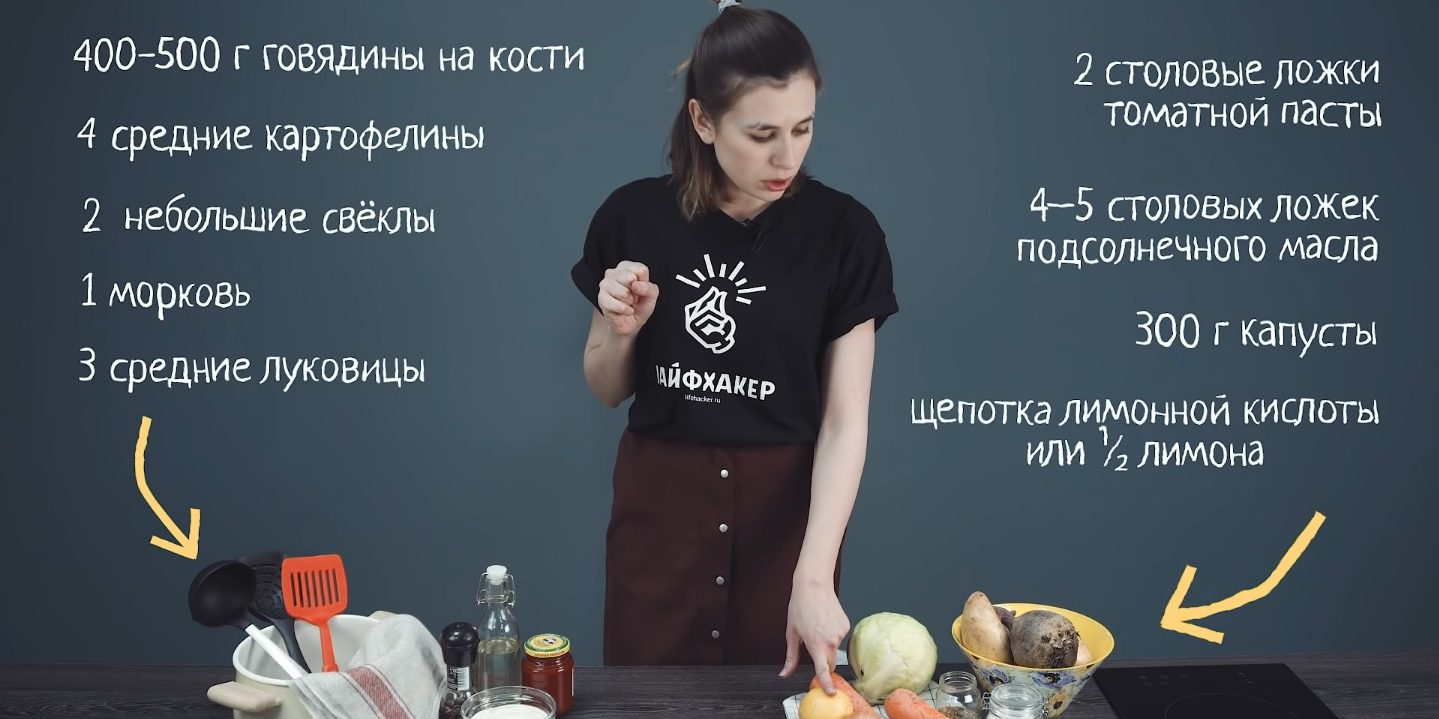
\includegraphics[width=0.75\textwidth]{img/borsch-e1568359200134.jpg}

Для бульона:
\begin{itemize}
    \item 1.5-2 л воды;
    \item400–500 г свинины или говядины на кости.
\end{itemize}


Для зажарки:
\begin{itemize}
    \item 2 небольшие свёклы;
    \item 1 средняя морковь;
    \item 3 средние луковицы;
    \item 4–5 столовых ложек растительного масла;
    \item щепотка лимонной кислоты, немного столового уксуса или ½ лимона;
    \item 2 столовые ложки томатной пасты.
\end{itemize}


Для борща:
\begin{itemize}
    \item 300 г свежей белокочанной капусты;
    \item 4 средние картофелины;
    \item соль — по вкусу;
    \item 1–2 сушёных лавровых листа;
    \item зелень — по вкусу;
    \item 1 зубчик чеснока — опционально;
    \item щепотка молотой гвоздики — опционально;
    \item щепотка молотого чёрного перца — опционально.
\end{itemize}

\textbf{Шаг 1. Сварите бульон.} Налейте в кастрюлю холодную воду, выложите мясо и поставьте на средний огонь. Бульон будет вкуснее, если использовать именно мясо на кости.

Следите за бульоном, перед закипанием снимите пену.

Когда жидкость закипит, накройте кастрюлю крышкой и варите на медленном огне час-полтора.

\textbf{Шаг 2. Сделайте зажарку.}
Вымойте и почистите свёклу, морковь и лук. Свёклу натрите на крупной тёрке, а морковь — на средней. Лук нарежьте небольшими кубиками.

Налейте масло в сковороду, включите средний огонь. Обжаривайте лук и морковь, помешивая, около 5 минут.

Затем выложите свёклу. Добавьте к ней лимонную кислоту, уксус или сок лимона. Благодаря этому борщ будет по-настоящему красным и приобретёт приятную кислинку.

Готовьте зажарку ещё 5 минут. После этого добавьте томатную пасту, перемешайте и оставьте на огне ещё на 5–7 минут.

\textbf{Шаг 3. Соберите борщ.}
Когда бульон сварится, выньте из него мясо. Пока оно остывает, засыпьте в кастрюлю нашинкованную капусту. Через 5–10 минут добавьте нарезанный соломкой или кубиками картофель.

Порядок закладки овощей можно менять. Если капуста молодая, её лучше добавить уже после картошки. Ну или одновременно, если ваш сорт картофеля разваривается быстро.

Пока варится картофель, отделите мясо от кости и нарежьте кубиками. Верните его в суп. Посолите по вкусу.

Добавьте зажарку и перемешайте.

Закиньте лавровый лист и мелко порубленную зелень. Накройте кастрюлю крышкой и варите ещё 5–7 минут.

Для аромата можно добавить в кастрюлю немного измельчённого чеснока, молотой гвоздики или чёрного перца. Оставьте борщ под крышкой настаиваться 5–10 минут.

\textbf{Как подать борщ на стол.} Борщ можно есть сразу после приготовления. Но, как правило, на следующий день он ещё вкуснее.

Добавьте в тарелку сметану и свежую зелень. Если предпочитаете покислее, положите дольку лимона.

Подайте к борщу ржаной хлеб или сдобные булочки, натёртые чесноком. Также блюдо прекрасно дополнят сало и пампушки.


\newpage
\section{Баклажаны Имам Баялды}


 {\it Источник: \url{https://www.gastronom.ru/recipe/46930}}

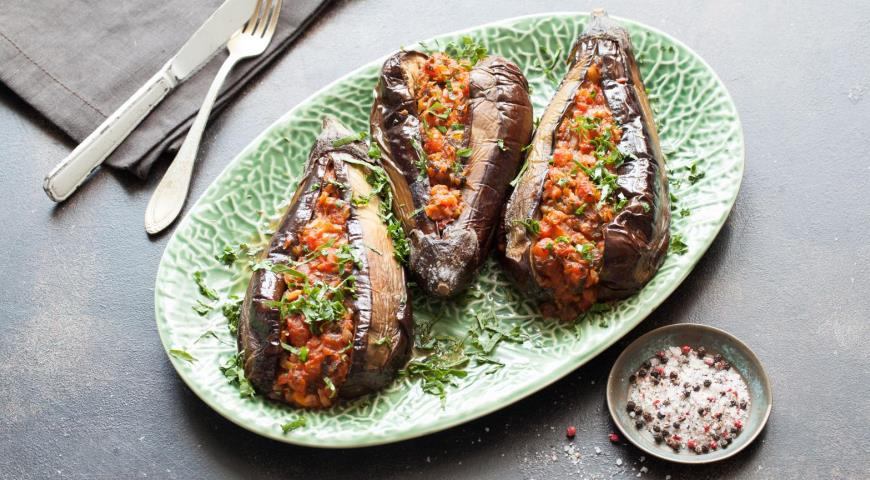
\includegraphics[width=0.75\textwidth]{img/baildi.jpg}

Баклажаны Имам Баялды популярно в турецкой, а также болгарской, армянской, греческой и других кухнях Балканского региона. Название переводится буквально как «имам упал в обморок». А вот причина его падения расходится от легенды к легенде. По одной версии он упал от аромата блюда, по другой – узнав цену. Третья же версия рассказывает о том, что женившись на девушке имам получил в приданное 12 кувшинов лучшего оливкового масла.12 дней девушка угощала мужа баклажанами с помидорами, а на тринадцатый не увидев блюда на столе, имам упал в обморок, поняв, что приданного больше нет.

\textbf{Ингридиенты.} 6 баклажанов (около 900 г);
2 средние красные луковицы;
4 зубчика чеснока;
5–6 веточек петрушки;
1 сладкий зеленый перец;
4 средних помидора;
1 ч. л. сахара (по желанию);
1 ч. л. молотой зиры;
1 ст. л. томатной пасты;
4 ст. л. оливкового масла;
соль;
свежемолотый черный перец.

% ПОШАГОВЫЙ РЕЦЕПТ ПРИГОТОВЛЕНИЯ
\textbf{Пошаговый рецепт приготовления}

Шаг 1. Разогрейте духовку до 220 °С. Застелите противень фольгой или пергаментом и смажьте оливковым маслом.

Шаг 2. Используя овощечистку, срежьте часть кожи баклажанов, чтобы получились широкие полоски. Надрежьте баклажаны вдоль, но не прорезайте их полностью. Посолите баклажаны внутри и снаружи, затем положите их в дуршлаг и оставьте на 30 мин.

Шаг 3. Положите баклажаны на противень и запекайте 20 мин.

Шаг 4.  Очистите лук и чеснок и мелко нарежьте. Измельчите петрушку. У сладкого перца удалите семена и перегородки, нарежьте кубиками. Помидоры надрежьте крест-накрест и положите в миску, залейте кипятком на 2 мин., затем обдайте холодной водой. Снимите кожицу, мякоть мелко нарежьте.
Подпишитесь на рассылку рецептов и советов
Подписаться


Шаг 5. Разогрейте в сковороде 2 ст. л. оливкового масла и обжарьте лук до мягкости. Добавьте перец и чеснок и продолжайте жарить еще 7–10 мин., посолите и поперчите. Положите помидоры и томатную пасту, зиру и петрушку. Если нужно, добавьте сахар. Тушите 5 мин. и снимите с огня.

Шаг 6. Уменьшите температуру духовки до 180 °С. Положите баклажаны в форму для запекания и наполните томатной смесью. Сбрызните оливковым маслом, добавьте 2 ст. л. воды в форму и выпекайте 40–45 мин.

Шаг 7. К концу приготовления баклажаны должны быть практически плоскими, а жидкость в форме должна почти выпариться. Подавайте баклажаны теплым или полностью остывшими.

\textbf{Пошаговый рецепт приготовления}

Шаг 1. Вскипятите 2,5 л воды, посолите и опустите спагетти. Варите пасту до упругости согласно инструкции на упаковке, примерно 6-7 мин. Откиньте на дуршлаг, дайте стечь воде.

Шаг 2. В глубокой сковородке разогрейте оливковое масло и обжарьте нарезанный ломтиками чеснок, 30 сек. Добавьте нарезанную соломкой ветчину и готовьте 3 мин.

Шаг 3. Соедините желтки со сливками и взбейте венчиком. Добавьте соль, свежемолотый черный перец, тертый пармезан и мелко нарезанный базилик, тщательно перемешайте.

Шаг 4. Переложите спагетти в сковородку с ветчиной, перемешайте и прогрейте, 1 мин. Разложите пасту карбонара с ветчиной и сливками в подогретые тарелки и полейте сливочным соусом.






\newpage
\section{Паста карбонара с ветчиной и сливками}


 {\it Источник: \url{https://www.gastronom.ru/recipe/53070}}

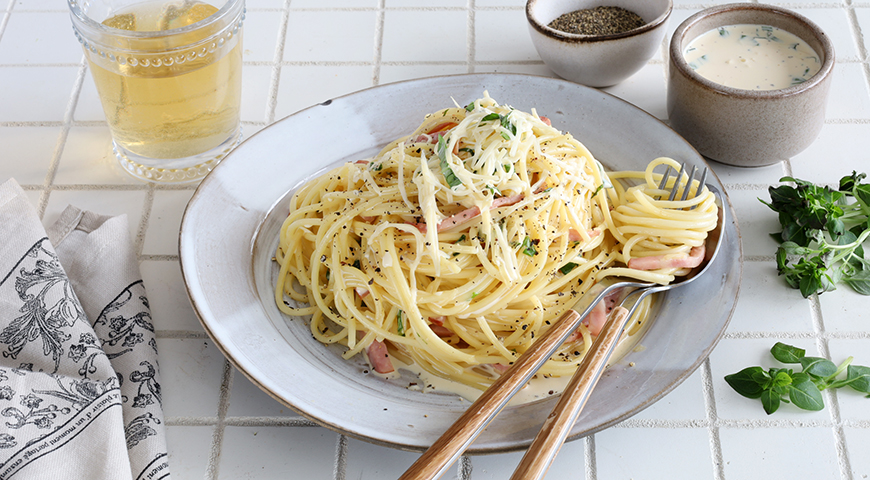
\includegraphics[width=0.75\textwidth]{img/carbonara.jpg}

Паста карбонара с ветчиной и сливками — один из вариантов приготовления этого знаменитого блюда. Поборники традиций, конечно, будут недовольны столь вольным обращением с классикой, однако к подобным кулинарным фантазиям сами итальянцы относятся довольно спокойно. Тем более что паста карбонара, приготовленная по этому рецепту, получается действительно очень вкусной и, как ей полагается, сытной. Сливки придают соусу приятную нежность, которую непременно оценят ваши близкие. Что касается ветчины, мы бы очень рекомендовали использовать сырокопченую: с ней паста карбонара станет значительно вкуснее.

\textbf{Ингредиенты.}
400 г спагетти;
200 г ветчины;
150 мл сливок жирностью 22\%;
2 сырых желтка;
50 г тертого пармезана;
2 ст. л. оливкового масла;
2 веточки базилика;
свежемолотый черный перец;
соль;
2 зубчика чеснока.
\chapter{Культ успеха}

\section{Что такое культ успеха}

\textit{Что такое культ успеха и как отличить свои желания и цели от навязанных?}

\textit{Источник: \url{https://happymonday.ua/ru/chto-takoe-kult-uspeha}}

\textit{Катерина Вольська}

Наш ритм жизни все ускоряется, мы торопимся получить больше денег, выше должность, лучше машину, больше новых гаджетов, книг, тренингов — всего больше. Казалось бы, это вполне естественные желания. Мы же хотим быть успешными и счастливыми, хотим развития — значит, с нами все в порядке. В теории мы все абсолютно правы. Но на практике это выливается в стремление достичь всего и сразу.

\begin{fancyquotes}
    Причем это «все» зачастую нам предлагают извне  — маркетологи, таргетологи, менеджеры по продажам или наше собственное окружение.
\end{fancyquotes}

Это становится похоже на какую-то игру в успех. Со всех сторон нам подбрасывают новые условия этой игры и уверяют, что просто необходимо еще чего-то достичь, еще что-то попробовать и приобрести. Как только мы видим триггер — то, что запускает в нас желание получить еще больше, — то включаемся в погоню за успехом. А в ней нет времени анализировать свои потребности, мотивы, желания — игрок должен быстро бежать к общепринятым «стандартам» успеха, не думая о том, что из этого всего ему действительно интересно и нужно.

Самыми распространенными такими «стандартами» считаются:

\begin{enumerate}
    \item стать СЕО компании к 25-ти годам;
    \item открыть свой бизнес до 30 лет;
    \item жениться/выйти замуж до 25 лет;
    \item родить ребенка/детей до 30 лет.
\end{enumerate}

Знакомо? Согласитесь, что все эти «стандарты» давят — на кого-то в большей степени, на кого-то в меньшей. Давят и заставляют жить в стрессе, если их не проработать.

\textbf{Что такое культ успеха?}

Иногда мы так заняты погоней за успехом, что упускаем что-то действительно важное — то, на чем строится наша жизнь.

Давайте представим, что ваша жизнь — это дом. Его фундамент — это ваш осознанный подход к жизни, решения, цели, желания и выборы. Уделяя этому время, вы закладываете фундамент своего дома. Конечно, дальше вы будете строить стены, крышу, делать ремонт, ухаживать за газонами у дома и создавать уют. Но фундамент — прежде всего.

А теперь представьте, что из-за давления социума вы купите первые попавшиеся стройматериалы, доверите фундамент каким попало строителям и побежите выбирать краску для стен. Или покупать рассаду, потому что прочли пост друга в Facebook о прекрасной клумбе у его дома и срочно хотите себе такую же. В итоге ваш дом рушится, потому что стоит он все-таки на фундаменте, а не на клумбе.

В этом и заключается культ успеха — мы очень быстро хотим получить результат, «как у других», соответствовать планке семьи, друзей и всех тех, кто присутствует в нашем реальном и виртуальном мире. Мы постоянно хаотично мечемся между целями, потому что нам «тоже так надо». Но надо ли действительно?

Речь не о том, чтобы перестать стремиться к росту и развитию. Речь о том, что постоянная гонка и неудовлетворенность собой, своей жизнью, работой, бизнесом, семьей и обесценивание того, что у вас есть, становится эпидемией.

\begin{enumerate}
    \item Одноклассник занимает руководящую должность в крупном холдинге!
    \item Подруга отдыхает 3-4 раза в год!
    \item У знакомых уже семья!
    \item Друга повысили на работе!
    \item У знакомого свой бизнес в 24 года!
    \item Однокурсник зарабатывает \$Х в месяц!
    \item Одноклассница похудела на 10 кг!
    \item Родственница сменила сферу деятельности и теперь работает удаленно и с гибким графиком за те же деньги!
\end{enumerate}

Вся эта информация, доступная нам 24/7, всячески способствует формированию культа успеха. Посты в социальных сетях, рассказы знакомых и бесконечный поток информации в Google и YouTube — все создано, чтобы вы пополняли свое информационное поле и сравнивали себя с другими.

\begin{fancyquotes}
    В свою очередь, другие люди также имеют в своем поле людей, с которыми сравнивают себя. И так по кругу. Мы все строим фейковые дома, которые могут рухнуть в любой момент.
\end{fancyquotes}

Можно обойтись косметическим ремонтом, если повезет. Быстро восстановить силы и ресурсы, подкорректировать образ жизни, привычки и укрепить дом. Сфокусироваться на важном и перестать распыляться.

Можно сделать капитальный ремонт — здесь предстоит серьезная работа над собой, своими ценностями и, возможно, длительная стадия возвращения потерянного и упущенного в гонке за успехом. Для этого необходима пауза и осознание полученного опыта для корректировки своего пути.

А может быть, придется строить новый дом с нуля. Это будет длительный процесс поиска потерянных смыслов и опор. Я использую метафору и сравниваю успех с постройкой дома, но его реконструкция может обернуться настоящим кризисом в реальной жизни. Речь идет о физическом, эмоциональном, духовном истощении и необходимости обратиться к психотерапии.

\textbf{Как понять, что значит успех лично для вас?}

Важно отметить, что наше определение успеха может меняться в разные периоды жизни. Мы можем быть уверены, что успех — это новое место работы, смена профессии, увеличение дохода, отпуск, свадьба, улучшение здоровья, курсы, тренинги, но когда мы этого достигаем, у нас появляется новый образ успешного человека — и мы снова начинаем погоню.

Успех для каждого свой. Зачастую мы ассоциируем его с человеком, который реализовался и достиг своих целей. Скорее всего, он счастлив, ни от кого не зависит и свободно распоряжаться своим временем. Возможно, он достаточно много путешествует. Возможно, у него прекрасная семья. Наверное, его окружают такие же успешные люди. И, вероятно, этот человек никому не подражает — он может быть самим собой, знает, чего хочет, и двигается к своим целям. Что из этого у вас ассоциируется с успешным человеком? А чего совсем нет в вашем списке критериев успешности?

Чтобы понять, где начинается и заканчивается именно ваш образ успешного человека, следует поднять свой уровень осознанности — задать себе неудобные вопросы и честно на них ответить.

\textbf{Упражнение №1}

\begin{enumerate}
    \item Напишите «Для меня успех — это ...».
    \item Напишите «Для других людей успех — это  ...».
    \item Напишите «На самом деле для меня успех — это ...».
    \item Ответьте на следующие вопросы.
\end{enumerate}

На кого из своего окружения я ориентируюсь? (Вы можете быть не знакомы лично). Кого я считаю примером для себя? (Вы можете быть не знакомы лично).
Какая / какие сферы жизни этого человека / этих людей являются для меня примером? Какие достижения этого человека / этих людей являются для меня примером? Чего я хочу из перечисленного выше?
Что за этим стоит, какую свою потрxебность я хочу этим закрыть?

\textbf{Упражнение №2}

А теперь представьте, что у вас уже есть все, что вы описали в упражнении выше, и ответьте на такие вопросы: Что из списка выше для вас действительно важно и ценно? Что из этого вы можете убрать из своей жизни и чувствовать, что у вас все ок? Что из этого списка является самым важным? Что из этого списка является важным для вашего окружения (родители, семья, любимый человек, друзья, виртуальные друзья, подписчики)? Что из этого списка является важным только для вас? Почему именно это важно для вас?

\textbf{Как не дать чужим представлениям об успехе влиять на вашу жизнь?}

Какой бы крутой телефон вы не купили, через год он будет уже не очень, так как появятся новые модели. Какая бы интересная работа у вас не была, вы будете стремиться занять новую должность. Каким бы ярким не был ваш отпуск — вам захочется так, как на фото у знакомых.

{\it
«Я буду успешен, когда …» — это парадокс той самой гонки за успехом.
}

Мы перестаем ценить момент, в котором находимся, перестаем ценить то, что у нас уже есть. Мы обесцениваем наши достижения, потому что нам всегда есть с кем себя сравнить и понять, что мы все еще недостаточно хороши.

\begin{fancyquotes}
    Если речь идет о вдохновении результатами других — прекрасно! Тогда это мотивация двигаться вперед. А если нет? Если вами движет страх быть хуже других или зависть?
\end{fancyquotes}

Можно ведь просто порадоваться за чужие достижения, правда? Но вместо этого мы чаще всего воспринимаем чужой успех как свой провал.

Чтобы минимизировать влияние чужого успеха на свою жизнь и сконцентрироваться на собственном желаемом успехе, выполняйте простые упражнения каждый день. Для этого вам понадобится от 5 до 15 минут.


\begin{enumerate}
    \item Опишите жизнь, о которой вы мечтаете, и перечитывайте описание каждый день. Если вам захочется внести корректировки, когда что-то станет неактуальным, делайте это. Но обязательно фокусируйте себя сами. Иначе это сделают за вас.
    \item Пишите 3-5 благодарностей каждый день — себе, близким, Вселенной, кому угодно. Фокусируйте себя на позитивных моментах — это прибавит вам энергии и напомнит о том, что хорошее уже есть в вашей жизни. Наверняка его очень много, и совсем не обязательно бежать туда, где трава кажется зеленее.
    \item Записывайте 3-5 своих успехов каждый день — что хорошего вы сделали, что получилось, что начали делать, кого порадовали и так далее. Фокусируйте себя на достижениях — это придаст вам уверенность в себе и своих силах, избавит от иллюзии, что вы застряли и не двигаетесь так быстро, как все вокруг.
    \item Следите за своим информационным полем — окружением, семьей, социальными сетями, рекламой и т.д. Но всегда сверяйте свой вектор движения со своими настоящими критериями успешного человека. Уделяйте время своему фундаменту — «подправить» его и сделать косметический ремонт намного легче, чем строить новый дом.
\end{enumerate}

И не забывайте, что всегда будет кто-то лучше, успешнее, счастливее, богаче, стройнее и так далее. Всегда! Но только от вас зависит, как на это реагировать: завидовать и заниматься самобичеванием, впрячься в гонку за успешным успехом (возможно, даже не своим) или вдохновляться и идти собственным путем.И не забывайте, что всегда будет кто-то лучше, успешнее, счастливее, богаче, стройнее и так далее. Всегда! Но только от вас зависит, как на это реагировать: завидовать и заниматься самобичеванием, впрячься в гонку за успешным успехом (возможно, даже не своим) или вдохновляться и идти собственным путем.
% \chapter{Работа, Карьера и Профессии}

\section{Устройство на работу}
Закончив университет и получив диплом юриста, я решил начать искать подходящую по специальности работу.

К сожалению, у меня сразу не получилось занять высокий пост.
Все как в один голос твердили, что у меня недостаточно практики, поэтому сначала н\'{у}жно получить практические знания и поработать несколько месяцев стажером.

Я так и сделал.
Посетив одну фирму в обрабатывающей промышленности, мне очень понравился не только коллектив и месторасположение компании, но и уровень заработной платы и перспектива роста.
Именно поэтому я принял для себя решение получить эту работу, чего бы мне это ни стоило.
Как оказалось, что сделать это было не так-то просто.

Сначала н\'{у}жно было поработать один месяц бесплатно, а потом целых три месяца стажером.
Работая стажером, я получал 30\% от зарплаты.

Эта сумма не была велико, но в то же время мне хватало этих денег на еду, оплату коммунальных услуг и на простые развлечения.

По происшествии 2 месяцев, работодатель заметил мое трудолюбие и талант, поэтому повысил мне зарплату еще на 20\%.

Я был безумно рад этому событию. Прошло 4 месяца и мне предложили полную ставку.
Для этого я заполнил анкету, прошел тест и ознакомился с новыми условиями работы.

К счастью, они были очень выгодными --- премии, надбавки за сверхурочные, оплачиваемый отпуск и оплачиваемые праздничные дни.

Я был на седьмом небе от счастья от такого предложения!

\section{Устройство на работу (2)}
Source: \href{http://irkzan.ru/home/gragd/soiskatel/soiskatelrabota.aspx}{Министерство труда и занятости иркутской области}.

Как начать поиск \explain{подходящего}{suitable} места работы? Как найти интересную работу и одержать победу в конкуренции с другими кандидатами? Для ответа на эти вопросы необходимо помнить:

\begin{itemize}[noitemsep, label=--]
    \item процесс поиска работы Вы должны взять в свои руки, \explain{проявляя}{exhibiting; showing} активность и инициативу;
    \item не ограничивайтесь одной специальностью, составьте список работ, который Вы можете выполнять;
    \item \explain{если Вы определили}{if you have identified} для себя какую работу вы ищете, рассказывайте об этом всем вокруг. Чем больше людей знают об этом, тем лучше;
    \item занимайтесь поиском работы 8 часов в день, считая это свой работой;
    \item работодатели стремятся \explain{нанимать}{to hire} победителей. Будьте уверены в себе, умейте подать себя;
    \item \explain{настройтесь}{tune in (to the fact)} на то, что Вы можете получить десятки \explainDetail{отказов}{отказ}{failure} --- это нормально;
    \item \explain{очередной}{next; following} отказ не должен выбивать Вас из колеи, а наоборот, пробуждать к дальнейшему поиску работы.
\end{itemize}

Современный рынок труда очень специфичен. Каждая сторона --- продавец и покупатель --- старается создать ситуацию выбора для себя: специалист, решивший сменить работу, как правило, \explain{рассматривает}{considers} несколько \explainDetail{предложений}{предложение}{offer} от работодателей, несколько вариантов работы, чтобы выбрать те \explain{условия}{conditions} работы, которые его больше \explain{устраивают}{satisfy} и, одновременно --- продать себя как можно дороже. Работодатель также проводит тщ\'{а}тельный отб\'{о}р кандидатов на рабочее место, чтобы \explain{приобрести}{to acquire} товар как можно лучшего качества и как можно дешевле.

Прежде всего, необходимо установить контакты с рынком труда, поскольку работодатель сам не придет к Вам со своими предложениями. Заставьте информацию работать на себя. Расскажите о том, что Вы ищете работу сослуживцам, родственникам, знакомым, соседям, бывшим одноклассникам и однокурсникам, преподавателям и администраторам учебных заведений, в которых Вы учились и др.

Стоит заглянуть в раздел объявлений в газетах. Прежде всего, обратите внимание на объявления тех фирм, которые указывают свое название, а не выступают обезличенно, скрываясь за абонентным ящиком или ничего не говорящим «организации требуются». Зная, о какой фирме идет речь, Вы можете навести о ней справки и потом решать, стоит ли пытаться попасть в нее. Ни для кого не секрет, что благополучные предприятия не нуждаются в рекламе, и люди, приходят на них сами, чаще всего по рекомендации. Адреса таких предприятий можно взять из специализированных журналов, отраслевой справочной литературы, наконец, просто из телефонных справочников.

Следующим этапом поиска может стать «прозвон» газетных предложений. При общении с работодателем необходимо:

быть вежливым, голос должен быть уверенным;
рядом иметь ручку и листок бумаги для записи необходимой информации;
отвечать на вопросы быстро и кратко, договориться о встрече.

\subsection{Резюме и его роль в трудоустройстве}
Грамотно составленное резюме демонстрирует умение излагать свои мысли на бумаге, умение оценить себя, умение исполнять предстоящие условия и работу. С помощью резюме можно информировать максимальное число работодателей о себе как о претенденте на вакантные рабочие места.

Правила составления резюме:

\begin{itemize}[noitemsep, label=--]
    \item резюме должно быть кратким (не более двух страниц);
    \item резюме должно включать только ту информацию, которая является значимой для работодателя;
    \item старайтесь не использовать сокращений.
\end{itemize}

Следует обязательно указать:

\begin{enumerate}[noitemsep]
    \item \textit{Ф.И.О.}, домашний адрес, контактный телефон. (Резюме, содержащие только адрес электронной почты, обычно не рассматриваются.
    \item \textit{Цель}. Название позиции на которую претендуете. Укажите должность, на которую Вы претендуете. Бывает, что соискатели указывают сразу несколько возможных вариантов трудоустройства, когда варианты имеют близкие функциональные обязанности. Например: «Ищу работу секретаря-референта, офис-менеджера, менеджера по работе с клиентами».
    \item \textit{Образование}. Необходимо указать полностью название учебного заведения, дату поступления и его окончания, специальность. Если высшее образование уже получено, не стоит упоминать о дате окончания средней школы. Если Вы получили дополнительное образование (закончили курсы, прошли тренинги), не перечисляйте все подряд, а только то, что имеет непосредственное отношение к профессии.
    \item \textit{Опыт работы}. Необходимо указать дату поступления и окончания работы, наименование организации, профиль ее деятельности, название должности и краткое описание должностных обязанностей и достижений в хронологическом порядке, начиная с последнего места работы.
    \item \textit{Профессиональные навыки}. В графе указывается знание и степень владения иностранными языками, знание специальных компьютерных программ текстовых редакторов, наличие водительских прав.
    \item \textit{Дополнительная информация}. В графе указывается наличие загранпаспорта, наиболее сильные черты характера и т.д.
    \item Укажите на возможность предоставления рекомендаций.
    \item Вся информация, содержащаяся в резюме, обязательно должна быть достоверной.
\end{enumerate}

\subsection{Пример резюме}
Петров Владимир Петрович

663000 г. Иркутск, ул. Российская,82 кв 16 тел. 33-56-78

\textbf{Цель}: Получение должности коммерческого директора в торговой компании

\textbf{Образование}:

\begin{itemize}[noitemsep, label=--]
    \item 1990-1995 Иркутская государственная экономическая академия. Инженерно-экономический факультет. Диплом инженера-экономиста
    \item 1996-1997 Курсы английского языка при Лингвистическом университете.
    \item 1998 Курсы по маркетингу при учебном центре ИГЭА
\end{itemize}


\textbf{Опыт работы}:

\begin{itemize}[noitemsep, label=--]
    \item 3.1998 --- н/время Фирма «Плюс» (Россия г. Иркутск) начальник отдела продаж.
          Оптовая торговля продовольственными товарами
          (консервы, сухие супы)\\
          Функции: организация продаж, контакты с розничными
          торговыми предприятиями, составление договоров, контроль за
          расчетами. В подчинении 3 человека. За период работы
          расширил сеть торговых точек с 17 до 60.


    \item 8.1995 --- 3.1998 ИЧП «ФОБОС», коммерческий агент.
          Розничная торговля продовольствием и ТНП.\\
          Функции: реализация товара через торговые точки фирмы.
          В 1996 г оборот фирмы достигал 3,5млн. руб. в год
\end{itemize}




\textbf{Дополнительные сведения}:
\begin{itemize}[noitemsep, label=--]
    \item Английский язык (могу изъясняться и работать с профессиональной документацией)
    \item РС --- пользователь (WinWord, Exel). Водительские права кат.В Опыт вождения 4 года. Имеется личный автомобиль.
\end{itemize}




% ----
\subsection{Собеседование с работодателем}
Пришел положительный ответ с предложением явиться на собеседование. Теперь главное --- произвести хорошее впечатление.

\textbf{Подготовка к собеседованию}.

А) Предоставляемые документы

В большой степени решающим для достижения успеха в поисках работы имеют внешний вид предоставляемых документов. Испачканные или порванные документы заставляют читающего их человека предположить, что кандидат в работе также неряшлив и несобран.

Для руководителя отдела кадров, как показывает практика, важнейшим документом, который помогает быстро ознакомиться с личностью кандидата, является автобиография, которая должна быть отпечатана на машинке.

В настоящее время все большее число фирм требует от кандидатов на должность, наряду с другими документами, заполненную личную анкету, которая смогла бы дать ответы на все вопросы, связанные с его первичной оценкой. Специфические условия каждой фирмы заставляют их включать в анкету соответствующие этим условиям вопросы. Фирма придает различное значение тем или иным качествам кандидатов, что и находит отражение в содержании анкеты. Содержание анкеты определяет также постоянно меняющееся положение на рынке труда.

Б) Внешний вид

Оденьтесь так, чтобы Вам было прежде всего удобно и Вы чувствовали бы себя свободно и уверенно, а не как на торжественном приеме у английской королевы. Женщины не должны усердствовать по части косметики и украшений. Не рекомендуется также одевать короткие и узкие юбки и платья и выбирать духи с «навязчивым» ароматом. Тоже самое относится и к мужчинам в отношении лосьона после бритья. Костюм и рубашка должны гармонировать по цвету. Если Ваша работа предполагает наличие у Вас «легкости на подъем», частые поездки и вообще подвижность, можно выбрать для этой встречи спортивный стиль одежды: приличного вида свитер или джемпер с выпущенным воротничком свежей сорочки, спортивного покроя брюки или джинсы, легкая обувь. Не следует путать спортивный стиль со спортивной одеждой. И в Москве, и в Иркутске нередко можно встретить молодых людей, носящих «мастерку» с пиджаком, спортивный костюм в комбинации с рубашкой, галстуком и кожаными туфлями. Нелепо будет выглядеть мужчина, пришедший устраиваться в спортивном костюме даже фирмы «Адидас». Мнение, что цена костюма придает ему солидность, глубоко ошибочно.

До собеседования:
\begin{enumerate}[noitemsep]
    \item проверьте время, дату и путь;
    \item исследуйте компанию;
    \item отрепетируйте вопросы и ответы;
    \item подумайте, что вы оденете и как будете выглядеть
\end{enumerate}



% ----------
\subsection{Пять первых критических минут}
Много кандидатур на разные работы отвергают в течение первых пяти минут собеседования.

Критический момент наступает, когда Вы входите --- в Вашем внешнем виде не должно быть ничего, что может вызвать разочарование.

Лучший первоначальный подход --- это улыбнуться. Это неизменно побуждает дружелюбные чувства в человеке, улыбка дает нам почувствовать себя намного лучше и более уверенно.

Другие полезные подсказки, которые следует использовать в первые пять минут:

не выкладывайте ничего, что принесли с собой до того, как собеседник предложит Вам сделать это;
предоставьте собеседнику возможность первому протянуть Вам руку для рукопожатия;
не садитесь, пока Вам не предложат.


\textbf{Поза.}
Устройтесь удобно, сядьте прямо, но без \explain{напряжения}{напряжение}{stress; tension; voltage}.
Не облокачивайтесь и не кладите руки на стол собеседника.
Не разваливайтесь на стуле.
Вы будете выглядеть куда более представительно, сидя прямо, нога на ногу, ваши руки расслабленно лежат на коленях. Неплохо убедиться, что ваш стул отодвинут от стола собеседника, чтобы дать Вам свободу движений.


\subsection{Получение информации}
Собеседование проводится для того, чтобы обе стороны давали и получали информацию. Одна из главных установок --- получить всю нужную вам информацию о работе и самой организации. Никогда не соглашайтесь на работу, пока не убедитесь, что она Вам подходит.

Не надо:
\begin{enumerate}[noitemsep]
    \item извиняться за свой возраст, здоровье, недостаток опыта;
    \item перебивать собеседника;
    \item критиковать последнего работодателя;
    \item быть слишком фамильярным или самоуверенным;
    \item шутить, ругаться или курить.
    \item Типичные вопросы работодателей при приеме на работу
\end{enumerate}


Почему Вы хотите здесь работать?
\begin{enumerate}[noitemsep]
    \item Выполняли ли вы работу такого рода раньше?
    \item Что Вы делали с тех пор, как стали безработным?
    \item Почему Вы ушли с последнего места работы?
    \item Почему Вы так долго оставались без работы?
    \item Как долго вы намерены работать у нас?
    \item Чем Вы занимались на последнем месте работы?
    \item На каком оборудовании Вы работали?
    \item В чем заключаются Ваши сильные стороны?
    \item Каковы Ваши слабые стороны?
    \item Расскажите нам побольше о себе?
    \item Какую зарплату Вы хотели бы получать?
    \item Были ли у вас конфликтные ситуации на работе?
    \item Когда вы сможете приступить к работе?
    \item Каким образом Вы планируете добираться до работы вовремя?
    \item Есть ли у Вас какие-либо вопросы?
\end{enumerate}

После собеседования:
\begin{enumerate}[noitemsep]
    \item поблагодарите компанию за собеседование в кратком письме;
    \item если от работодателя не будет вестей, то позвоните и спросите, каков результат собеседования.
\end{enumerate}

Помните! В каждом из Вас есть внутренние резервы. Используйте их. Разбудите свою активность --- и успех будет в Ваших руках.

Желаем скорейшего трудоустройства!


\section{Виртуальный ассистент: профессия будущего}
Source: \href{http://www.cyprusmoms.com/virtualnyj-assistent-professiya-budushchego/}{www.cyprusmoms.com}.\\

Представьте ситуацию: вы живёте в стране, в которой не имеете возможности работать. Дети подрастают, хочется реализоваться профессионально, но идей для собственного бизнеса нет, да и времени свободного всего час-два в день. Знакомо?

Думаю, что я не одинока в таком положении. Живу на Кипре уже давн\'{о}, но разрешения на работу нет, да и найти работу в нашей деревне довольно сложно. Поэтому я начала думать об \explainDetail{удалённой}{удалённый/-ая}{remote} работе через интернет --- \explainDetail{вела}{вести/повести (веду, ведёшь, ведут)}{to lead} собственный блог, администрировала несколько групп в Фейсбуке для поддержки местного комьюнити, писала статьи, фотографировала, но не понимала, как перевести это хобби в \explainDetail{опл\'{а}чиваемую}{опл\'{а}чиваемый}{paid (from: оплачивать/оплатить)} деятельность.

Да, я читала рекламные статьи школ, которые онлайн обучают различным профессиям, но мне было непонятно, как потом находить работу, как работать с клиентами, чем \explain{зацепить}{to hook on; to catch (цепь: chain)} клиента, когда на рынке множество таких \explainDetail{новичков}{новичок}{newbie}, как я...

И вот, когда некоторое время назад я прочитала статью о профессии «Виртуальный ассистент», во мне щёлкнуло --- вот оно! То дело, которое я искала.

Кто такой виртуальный ассистент? Это универсальный специалист, который помогает предпринимателю вести бизнес в интернете --- наполняет страницы в социальных сетях, верстает лендинги и презентации, организовывает вебинары и налаживает \explainDetail{почтовую рассылку}{почтовая рассылка}{mailing list}.

В зависимости от предыдущего опыта, ассистент может специализироваться в том или ином направлении. Но в целом, это человек, который хорошо ориентируется в интернете, может найти нужный сервис, написать запрос, проконтролировать подрядчиков и быть тем многоруким многостаночником, который снимет с предпринимателя рутинные обязанности. И не важно, в какой стране живёт предприниматель и какое гражданство имеет Виртуальный ассистент --- они встречаются и сотрудничают в интернете.

{\it К 2020 году 20\% рабочих мест в России будут виртуальными, сказано в исследовании «J’son \& Partners Consulting», сделанном по заказу сервиса «Битрикс24». По данным исследований 2016 года эта цифра в Европе составляет 17\%, а в Японии и США доходит до 40\% от всех работающих.}

Я погуглила и поняла, что в англоязычной среде эта профессия очень распространена, даже существуют ассоциации бизнес-помощников.
На русскоязычном пространстве информации меньше, но есть несколько школ подготовки виртуальных ассистентов.
И все они --- что очень ценно --- обещают помощь со стажировками и трудоустройством. Результаты исследования школ, которые готовят бизнес-помощников, вы можете посмотреть на моей странице в фейсбуке Я остановилась на Международной школе подготовки бизнес-ассистентов и интернет-маркетологов «Helppy» Ольги Шевченко и ни минуты не пожалела. И организация обучения, и полезность информации --- на высоте!

Обучение длится пять недель, и погружение в учебу полное. За 35 дней ты вникаешь в принципы организации интернет-бизнеса, верстаешь презентацию в Пауэр Поинт, составляешь контент-план и график постов в рамках тобой же разработанной стратегии продвижения в соцсетях, верстаешь лендинг --- одностраничный сайт, а так же --- ТА-ДАМ! --- составляешь портфолио для самого себя. Понятно, что это не все темы, а только те, по которым требовалось сдать домашнее задание, и над которым мы все корпели ночами. На все домашки ты получаешь развёрнутые ответы, и очень редко удавалось сдать их с первого раза, спрашивали очень строго --- то типографика хромает, то дизайн подвёл.

Кроме лекций и обучающего материала, в закрытом разделе собрана база данных полезных статей, в секретной группе кипит жизнь --- кураторы и сокурсники обсуждают задания, а по пятницам Ольга Шевченко разговаривает с каждым курсистом отдельно и отвечает на все волнующие вопросы.

Создание портфолио --- это огромный пендаль собственной самооценке. После того, как ты соберешь всё, что ты можешь, применишь правила сильного текста, прикрутишь туда отзывы клиентов (мы делали домашнее задание по заказу интернет-предпринимателей, а они нам писали отзывы), подберёшь шрифты, а потом ещё сверстаешь это в лендинг с красивыми картинками... От этогосамооценка лезет вверх, и ты готова на подвиги и новые свершения. Хотите посмотреть на моё портфолио?Здесь. Я вам его показываю не для того, чтобы похвастаться, а для того, чтобы показать, что у вас может получиться на выходе.

Хорошо, что я начала учиться заранее, поэтому даже успевала спать и вести клиентов, которых нашла тут же, рядом с собой. Дело в том, что, начиная заниматься и вникать в тему, у тебя обостряется зрение и ты видишь, что в этом проекте, например, ты можешь быть полезной, а здесь ты можешь докрутить страницу и получить совсем другие результаты. Ты предлагаешь свои услуги, показываешь, что можешь сделать, как можешь помочь, и люди откликаются. Я и многие сокурсники именно так получили работу.

Я не обещаю лёгкой жизни --- учиться и работать надо будет много, информация в интернете меняется быстро, у Фейсбука, например, нововведения каждую неделю, ежедневно на рынок труда выходит всё больше людей. Надо будет выстраивать свой график работы и думать о тайм-менеджменте. Например, черновик этой статьи я набирала на телефоне в гугл-кипе в то время, пока мастер педикюра работала с моими ногами. А от одного, очень перспективного предложения пришлось отказаться, потому что я понимала --- или работа, или семья, третьего не дано, со всем в данный момент не справлюсь.

Профессия виртуального ассистента --- хорошая ступенька для тех, кто выходит из декрета и живёт в том месте, где устроиться на работу сложно. Это профессия для того, кто умеет работать с большим количеством информации и в состоянии организовать рабочие процессы и самого себя. А дальше можно покорять новые вершины, и истории выпускников школы тому подтверждение.

Удачи!

\section{Правила деловой переписки}

\textit{Источник: \url{https://4brain.ru/blog/pravila-delovoj-perepiski/}}

В информационном веке важно обладать умениями и навыками общения в сети Интернет. С одной стороны, письменная речь основывается на тех же правилах, что и устная, с другой, в отдельных направлениях есть необходимость использовать особые приемы, чтобы заочно, не видя собеседника, выстроить с ним правильную коммуникацию и быстрее прийти к нужному результату, используя минимум слов и писем.

Управленцам, менеджерам, редакторам, маркетологам – правила деловой переписки необходимо знать всем. Заинтересовать собеседника, получить результат от взаимодействия с ним можно только при правильном подходе. Стоит учитывать, что при удаленном контакте, когда собеседники не видят друг друга, отсутствует визуальный контакт и возможность использовать множество слов.

В данном случае краткость-сестра таланта – это одно из главных правил продуктивной переписки. Не всегда люди имеют возможность читать длинные письма, поэтому мысли нужно излагать максимально точно и лаконично.

В деловой электронной переписке есть общепринятые правила, грамотно используя которые можно не переживать, что письмо отправится в «Спам». Они подробно изложены в книге создателя сервиса «Главред» Максима Ильяхова «Новые правила деловой переписки», которая считается лучшим пособием в своем роде в России. Соавтор Людмила Сарычева – автор статей о деловом общении.

Опираясь на книгу, мы расскажем о том, как освоить правила деловой переписки, в чем они заключаются и выясним, зачем они вообще нужны, если можно просто излагать свои мысли, чтобы удаленно изъясняться с собеседником.

А чтобы научиться лучше взаимодействовать с людьми и подтянуть или развить навыки общения, рекомендуем пройти нашу программу «Лучшие техники коммуникации». Полученные знания будут полезны в письменной, устной речи, при взаимодействии с коллегами, партнерами и т.д.

\textbf{Типичные ошибки авторов}

Казалось бы, что сложного в том, чтобы написать письмо и, как кажется, договориться с собеседником на расстоянии о чем угодно. В этом как раз кроются типичные ошибки обывателей, чьи письма часто отправляются в «Спам».

На основе материалов, изложенных в книге Максима Ильяхова «Правила деловой переписки», разберем основные проблемы писем, которые буквально лежат на поверхности и видны сразу [М. Ильяхов, 2018]:
\begin{enumerate}
    \item В письме нет темы. Предположим, у адресата большая нагрузка на работе и просматривать почту оперативно он не может. За день на его ящик придет, например, двадцать писем. Каждое нужно прочитать, обработать. Представляете, сколько времени потребуется на чтение? Соответственно заголовок письма обозначит, что внутри, а значит, послужит своеобразным маяком для читающего. Идеальное решение – сделать такой заголовок, который полностью отражает смысл письма. В книге также дана рекомендация помещать в теме такие подробности, которые обозначат, стоит ли читать письмо сразу, какие действия необходимо предпринять для решения вопроса.

    \item «Уважаемые коллеги» --- типовой и очень распространенный шаблон, который, как оказывается, вызывает непонимание и не стимулирует концентрацию силы, а оказывает обратный эффект. Он звучит как «Коллеги, разберитесь сами, кто это сделает», а также не вызывает уважения из-за отсутствия адресата в обращении. Если нужно что-то сделать, решить вопрос, лучше написать конкретному человеку и дать ему подробную информацию, нужные вводные, а не делать коллективную рассылку. Такой подход гораздо эффективнее.

    \item Вторжение в свободное время человека без извинений. «Как проходит выходной / больничный / отпуск?» – эти вопросы точно вызовут раздражение, ведь человек вне рабочего времени занят своими делами. Если возникает острая ситуация, когда участие адресата все же необходимо, важно извиниться за вторжение и обосновать проблему, чтобы человек понял, что задачу решить нужно срочно.

    \item «У меня отличная новость!» По мнению Ильяхова, это дурная фраза, за которой обычно кроется не хорошая, а плохая новость, поэтому лучше сразу переходить к делу, а не создавать вид, что все хорошо.

    \item Абстрактные суждения без постановки конкретной задачи: «Надо бы сделать», «Я тут подумал» и подобные. Людей раздражает неопределенность во всех сферах жизни, в том числе и в постановке задач. Если сотрудник сам будет додумывать детали задачи, он рискует не попасть в мысль того, кто эту самую задачу ставит. В письме должны быть изложены все аспекты вопроса.

\end{enumerate}

Это основные ошибки, которые чаще остальных встречаются в письменной речи обывателей и приводят к медленному решению задач. В книге их перечислено больше: минимум вопросов в одной теме письма, не приложенные файлы, ошибки в обращении, чрезмерное использование шаблонных фраз и стоп-слов. Хочется отослать пишущего к еще одной книге Ильяхова «Пиши, сокращай» – меньше лишних слов, больше четкости и адресности, тогда письмо наверняка будет замечено и прочтено.

\textbf{Что раздражает читателя?}

А теперь поговорим о том, что раздражает читателя делового письма. С отсылкой к «Правилам деловой переписки», книге главреда.

\textbf{Небрежность}

Ошибки пунктуации, неверно составленные предложения, отсутствует подпись. Письма на скорую руку тоже должны быть написаны с умом, иначе получатель может подумать, что задача не первостепенная, раз так небрежно составлена.

\textit{Небрежный текст:} «Здравствуйте Михаил составте пожалуйста список сотрудников для согласования допусков на объект».

\textit{Как надо:} «Добрый день, Михаил! Прошу Вас составить список сотрудников для согласования допусков на объект до 15 января. Директор отдела».

Как видно, в первом предложении есть ошибки орфографии и совсем отсутствуют знаки препинания. Во втором случае просьба оформлена точно, есть обращение, дедлайн, подпись.

\textbf{Панибратство}

Оно выражается в пренебрежительном обращении, например, «народ», «приветик» без соблюдения субординации. Подобное обращение вызывает лишь отторжение, но не самими словами, а нарушением личных границ тех, к кому оно адресовано. Подобное допустимо в неформальной обстановке, но не на работе.

\textbf{Перекладывание ответственности и создание групповых переписок}

В групповых переписках, в которых есть неадресные обращения, никто не понимает, кому полагается решение задачи. Это распространенная проблема в больших коллективах при отсутствии грамотных управленцев.

Как не надо: «Коллеги, нам нужно обсудить вопросы размещения рекламы на сайте партнеров. Какие предложения?»

Как надо: «Сергей, примите решение, стоит ли размещать рекламу у партнеров – обещают 1 млн просмотров. Медиаплан в приложении».

Как идентифицировать сотрудника, который перекладывает ответственность? Он использует такие фразы: «передам коллегам», «это не в моей компетенции», «жду решения руководства». За ними скрывается «сами внесите правки, я в этом не участвую, не трогайте меня».

\textbf{Неуместность фраз и бездумное употребление сокращений}

Случается такое, что отдельные сотрудники используют жаргонизмы и сокращения либо неуместно, т.е. без понимания их смысла, либо настолько часто, что не все коллеги понимают, о чем речь.

\textit{Пример:} «Проведите левкеридж лидеров мнений для повышения узнаваемости бренда и чекните в доке результат».

\textit{Перевод:} «Изучите, что думают эксперты о бренде и как можно повысить его узнаваемость. Результаты занесите в документ».

Какое предложение проще понять? [Top Lead, 2015].

\textbf{Неуважение к чужому времени}

Важное правило общения деловой переписки – не мешай другому делать свою работу. Слова «надо вчера», «это в приоритете», «ASAP» вышибают человека из своего режима. И все бы ничего, но если дело действительно срочное.

Часто бывает так: все бросишь, переключаешься, делаешь эту работу, а когда наступает «завтра», то уже и не так срочно было нужно. В результате время и силы потрачены почти зря. Чужое время – не расходный материал, поэтому относиться к нему следует ответственно и серьезно, а не использовать в качестве развлечения и инструмента повышения собственной крутости.

\textbf{Примеры от Максима Ильяхова:}

Сказали: «Коллеги, мы вас услышали». Как поняли коллеги: «Вы – сборище баранов, которые не знают, чего хотят. Мы презираем вас, но у вас есть деньги».

Сказали: «Это дело на пять минут». Как поняли коллеги: «Это дело на целый день, а то и на два».

Это основные ошибки деловой переписки, с которыми наверняка сталкивался каждый человек. Их главная проблема – это не используемые слова, а смысл, который за ними кроется. Умышленно или неумышленно заложенный – не важно.

\textbf{Зачем учить правила?}

Во-первых, правила деловой переписки по почте предполагают упрощение и улучшение коммуникации – никто (или почти никто) не хочет целый день тратить на написание писем в попытке объяснить адресату, чего от него ждут.

Во-вторых, знание правил ведения переписок помогает наладить отношения с окружающими в целом. Те, кто владеет навыками коммуникации, свободно общаются с разными людьми на любые темы.

Для погружения в тему деловой коммуникации книга «Новые правила деловой переписки» Ильяхова Максима, создателя сервиса «Главред», подходит идеально. Это одно из лучших профессиональных пособий в России. Она написана простым и понятным языком, автор приводит множество наглядных примеров.

Книга – учебник для менеджеров, маркетологов, секретарей, делопроизводителей, администраторов, всех специалистов, ведущих в той или иной мере переговоры по электронной почте.

Знание правил переписки дает несколько конкурентных преимуществ эксперту и его компании:
\begin{enumerate}
    \item Сообщения будут точными, запоминающимися, они не попадут в спам.
    \item Для решения вопроса понадобится минимум писем, а значит, и времени на решение задачи.
    \item Устраняются многословие, «вода», канцеляризмы, избыток в речи которых портит любую коммуникацию.
\end{enumerate}

Деловая переписка – это не реверансы из вымученных шаблонов, а минимум манипуляций и максимум эффективности.

\textbf{Основные правила правильной деловой переписки}

Рассмотрим основные постулаты деловой переписки, ее правила на примерах писем, обратившись к книге Максима Ильяхова. Кстати, многие из них перекликаются с основными рекомендациями Управления государственной службы и кадров Правительства Москвы, поэтому в эффективности их использования сомневаться не приходится [Университет Правительства Москвы, 2015].

\textbf{Уважение времени и внимания адресата}

Итак, первоочередные правила делового письма:
\begin{enumerate}
    \item Одно письмо – одно дело. Нет смысла умещать в одно послание множество вопросов. Во-первых, так их сложнее улавливать и перерабатывать. Во-вторых, это помогает структурировать и саму подачу вопроса – в одном письме точно не смешаются приложения, тезисы и прочие детали. К тому же, человеку не придется переключаться – это тоже работа, которая требует времени и сил.
    \item Назвать письмо в теме, чтобы адресат понял задачу, еще не открыв послание. Так он сможет расставить приоритеты при обработке писем. Заголовки оформляются точно и предельно емко. Например: «Акт сверки “Кристалл” III квартал», «Отчет посещаемости за январь 2022», «Выгрузка контактов, 15 февраля». В компаниях может быть принята своя система обозначения писем, например, «Черновик допсоглашения», «Внутренний план», «Вычитано, отчет», «Заявка на приемку» и т.п.
    \item Обозначить срочность – важный момент, если важно определить дедлайн выполнения задачи. Хорошо, если необходимая дата была читабельной и понятной без лишних телодвижений (например, поиска календаря и отсчета дней). Зашифрованный вариант: «Решить задачу к 17.04.2021», понятный вид: «Решить задачу до этого четверга».
\end{enumerate}

Важное дополнение: в некоторых компаниях электронная почта считается быстрым способом передачи информации, где сотрудники по инструкции по мере поступления проверяют почтовый ящик. Если в вашей компании этого нет, сверхсрочные задачи лучше обсуждать по телефону – это точно быстрый вариант. Формулировка «Сделать как можно скорее» или «Срочно» нерабочая, поскольку не содержит конкретики, а только неуважение к рабочему и личному времени адресата.

И далее переходим к самому интересному – составлению самого тела письма. Если с обозначением заголовка, постановкой даты все более-менее понятно, то с оформлением мысли могут возникнуть проблемы, а то и страх белого листа, когда не знаешь, с чего начать. Для таких случаев инструкция ниже.


\textbf{Структура письма}

Как в любом тексте, в деловом письме должны быть начало, середина и заключение. Пробегая глазами по сообщению, читатель должен понимать, где основная мысль, вопросы, заключения, ссылки, приложения. Располагают их обычно в таком порядке:
\begin{enumerate}
    \item Обращение с именем, приветствие.
    \item Основная смысловая часть, суть письма.
    \item Вопросы к читателю, лучше отдельными выделенными блоками.
    \item Призыв к действию, контакты, ссылки. Оставьте контакты, как с вами можно связаться помимо почты.
\end{enumerate}

Пример плохого оформления письма:

«Сергей, добрый день! Не смог прийти к Вам лично, приношу извинения. Пообщался с ребятами, хочу прояснить несколько моментов. Когда Вы планируете подать заявку на обучение? От этого будет зависеть срок подготовки документов нашим отделом. Кто сможет стать вашими поручителями? Консульство внимательно оценивает этих людей, поэтому их состав нам следует обсудить заранее. Какой график оплат Вам подойдет? Мы предлагаем внести предоплату 50%, но вуз позволяет внести от 15%. По нашему опыту, чем больше предоплата, тем выше шансы получить визу. В случае, если посольство откажет, вуз вернет деньги в полном объеме. Мы можем обсудить этот вопрос по телефону. Иван, +7 901 123-45-67».

Налицо все типичные ошибки: абзацев нет, разделения нет, много лишнего, вся информация в куче и плохо читабельна.

По правилам деловой переписки по электронной почте можно оправить сообщение в таком виде:

«Сергей, добрый день!

Не смог прийти к Вам лично, приношу извинения. Пообщался с ребятами, хочу прояснить несколько моментов.
\begin{enumerate}
    \item Когда Вы планируете подать заявку на обучение? От этого будет зависеть срок подготовки документов нашим отделом.
    \item Кто сможет стать вашими поручителями? Консульство внимательно оценивает этих людей, поэтому их состав нам следует обсудить заранее.
    \item Какой график оплат Вам подойдет? Мы предлагаем внести предоплату 50%, но вуз позволяет внести от 15%. По нашему опыту, чем больше предоплата, тем выше шансы получить визу. В случае, если посольство откажет, вуз вернет деньги в полном объеме.
\end{enumerate}

Мы можем обсудить эти вопросы по телефону.

Иван, +7 901 123—45-67».

Как говорится, найдите несколько отличий! Заметим, что в сообщении содержится несколько вопросов, но на одну тему, поэтому наш Иван сэкономил время адресата, предложил созвониться, проявил заботу о нем.

Если основная задача в большом объеме, старайтесь умесить ее в пару предложений, отбросив лишние слова, используйте списки, абзацы.

\textbf{Например:}

«Виталий!

У нас проблемы с коммутационными комплексами «Броненосец», поэтому Сергею или «Альфе» их не хватит. Тебе надо решить, кому сколько отдать до конца дня.

Почему так получилось: Сергей сделал заказ комплексов для собственного проекта и забирал их с нашего склада постепенно. На данный момент осталось 80 штук, из них для Сергея 40 комплексов, он заберет их завтра.

Для «Альфы» мы должны поставить 60 боксов, с ними мы ведем параллельный проект.

Получается, завтра нам не хватит 20 боксов для «Альфы» или Сергея.

Реши, пожалуйста, вопрос с Александром сегодня до 19:30, скажи мне, я передам складу, чтобы они подготовили к завтрашней выдаче.

Семен, менеджер по логистике.

+7 902 123-45-67».

Суть понятна, структурирована, разложена по блокам.

Если в письмо нужно вложить ссылки, сделайте это в столбик, тогда читателю будет достаточно нажать на нужную, чтобы открыть окно, а не копировать строки, вычленяя запятые и пробелы.

\textbf{Вежливость}

Важные аспекты хорошего письма: не путать имена, не злоупотреблять жаргонизмами и заботиться о читателе. Приветствуется краткость – чем меньше слов, тем менее раздражающим будет письмо.

Важно проявить заботу о читателе – разделить текст, чтобы он был читабельным, предложить варианты действий и возможных решений задач. Придерживайтесь нейтрального и спокойного тона изложения. Не пишите без необходимости, только чтобы напомнить о себе.

Вежливость не в словах, она в отношении.

\textbf{Формировка вопроса}

Правильно задать вопрос – это целая наука. Недостаточно собрать в предложение нужную информацию и поставить в конце вопросительный знак.

Деловое письмо, по правилам деловой переписки, должно содержать правильно поставленный вопрос. Никакой риторики и отвлеченных умозаключений. В некоторых книгах авторы рекомендуют задавать читателю открытые вопросы, например, «Что ты об этом думаешь?» Однако на такой вопрос ответить не просто сложно, не каждый сообразит, как к нему подойти, потому что конкретики в нем нет. Такой вопрос часто игнорируют с надеждой, что «само рассосется».

\textbf{Как не надо: }

«Мы получили 500 откликов, по которым будем составлять картину возражений. С другой стороны, эти люди будут ждать внедрения своих ожиданий в работу.

Мы можем поговорить с потенциальными клиентами, но для этого нам надо выделить сотню менеджеров. Возможно, благодаря этому мы сможем проработать свои скилы.

С другой стороны, наш диалог с текущими клиентами может напомнить «ошибку выжившего», ведь нам надо вести диалог с отказавшимися от сотрудничества клиентами. А как на них выйти – я не знаю, информации в CRM нету.

Что об этом думаешь?»

Гораздо удобнее ответить на конкретные вопросы, если бы их задали в рамках письма:

«Мы можем узнать более глубокие о себе вещи и прокачать скилы. Меня беспокоит, что наш диалог с текущими клиентами может напомнить «ошибку выжившего», ведь нам надо вести диалог с отказавшимися от сотрудничества клиентами. А как на них выйти – я не знаю, информации в CRM нету.

Какие у меня вопросы и сомнения:
\begin{enumerate}
    \item Опрос создаст резонанс в СМИ, а это нам сейчас точно не нужно.
    \item Как работать с ожиданием опрошенных клиентов?
    \item Что, если опросить ключевых клиентов приватно?
    \item Как нам выйти на тех клиентов, кто с нами уже не работает?
\end{enumerate}

Если тебе удобно, давай я тебе позвоню и все обсудим».

Из примеров видно, что по-разному поставленные вопросы предполагают совершенно разной точности ответы. Чем точнее сформулирован запрос, тем быстрее вы получите конструктивное решение от собеседника.

\textbf{Благодарность}

Поблагодарить собеседника иногда важно и нужно, но писать одно «спасибо» – неверное решение. Письмо придется открыть, прочитать, удалить, а особой ценности такое послание не несет. Чтобы исправить это, напишите конкретно, за что благодарите, прикрепите подарок:

«Марина, спасибо! Ты очень выручила нас! В знак благодарности прими курьера с подарком от нас, я попросил его оставить коробку в приемной на твое имя».

Если подарок уместен, продумайте, чтобы адресату он был нужен и удобен для перехвата – вряд ли человеку будет интересно бегать за курьером или караулить его, когда нужно выходить по делам.

Делать подарок необязательно, можно просто выразить благодарность словами и предложить свою помощь:

«Марина, спасибо! Ты нас очень выручила! Если тебе понадобится помощь в организации мероприятий, я буду рад сделать тебе хорошую скидку».

Не каждый протянувший руку помощи человек будет ждать благодарности в ответ, но этот жест, особенно подкрепленный приятным бонусом, определенно прибавит вам значимости.

\textbf{Извинения}

Нередко письмом нужно извиниться за неприятные инциденты. Самый частый повод – срыв сроков сдачи чего-либо. И все зависит от значимости провала.

Пример: «Дмитрий, привет! Я должен был сегодня прислать перевод текста, но не успел сделать его. Извини! Данил».

Человек пишет письмо с извинениями за срыв сдачи перевода в день дедлайна. Заказчик не может подписать договор или сделать публикацию, у него график. Что дадут ему извинения? Ничего, Дмитрию от извинений не станет легче. Данил проявил безответственность, не предложив вариантов выхода из ситуации.

Что он мог сделать:

\begin{enumerate}
    \item Предупредить о проблеме заранее, например, за день-два и договориться об отсрочке либо Дмитрий смог бы найти за это время другого исполнителя.
    \item Предложить решение проблемы, но, опять же. Заранее.
\end{enumerate}

«Правильное» извинение:

«Привет, Дмитрий!

В четверг я должен прислать перевод договора, но не успеваю ко времени. Чтобы не подводить тебя, я нашел переводчика, он готов сделать работу в среду, чтобы остался день на проверку, так я точно успею просмотреть результат. Таким образом, в четверг у нас будет готовый переведенный договор.

Вопрос в бюджете: стоить это будет 10 000 рублей. Мы сможем это оплатить?

Данил».

Не стоит бояться признаться в провале или срыве срока, своевременное извинение и нахождение решения поможет сохранить лицо, репутацию и добрые отношения с партнерами. Но и злоупотреблять этим определенно не нужно.

\textbf{Когда писать не надо}

Есть случаи, когда писать письма, даже очень срочные, не надо – есть все шансы допустить всевозможные ошибки, о которых сказано ранее. Таких ситуаций три:
\begin{enumerate}
    \item На эмоциях. В них поток мысли не структурирован и редко продуман, есть риск наговорить лишнего, нарушить субординацию. На радостях тоже можно натворить ошибок. Сначала успокойтесь, придите в «дзен» и только потом пишите письма.
    \item Вместо планерки. Групповые переписки в попытках что-то решить – это настоящее зло. Десятки людей, читающие одновременно письма и отвечающие на них, создают хаос в диалогах, в ответах теряется суть вопросов, как и сами ответы. Многие такие переписки проходят безрезультатно. Если планерка все же сорвалась, а задачи распланировать необходимо, следует собрать нужных людей в телефонной конференции или на локальном собрании, либо раздать задачи адресно, как уже говорилось ранее.
    \item Когда «горит». У сотрудников разная скорость переработки почты, ведь они обычно занимаются и другой работой тоже. Если задача требует очень быстрого решения, целесообразно не отправлять письма по электронной почте, а позвонить, чтобы не засорять ящик адресата десятком напоминаний «срочно», «пожар-горим».
\end{enumerate}

Еще один случай, когда писать не надо – когда мысли не структурируются, а вопрос очень важный и ставки высоки, для ошибок нет маневра. Возможно, в таком случае будет полезно:
\begin{enumerate}
    \item Проконсультироваться с коллегами, как структурировать материал.
    \item Провести аудиоконференцию.
    \item Организовать личную встречу.
\end{enumerate}

Личный контакт поможет лучше выстроить диалог, проследить за реакциями партнера, обговорить детали, которые в переписке можно упустить, а потом вляпаться в конфузную ситуацию.

\textbf{Холодные письма}

Для диалога с незнакомыми людьми, так называемыми «холодными контактами», выше перечисленные правила остаются актуальными, но есть несколько важных дополнений, которые помогут сделать переписку более продуктивной:
\begin{enumerate}
    \item Сохраняйте спокойный тон. Никаких эмоций, сохраняйте нейтральную тональность общения, как будто разговариваете с незнакомцем вживую. Соблюдайте субординацию, никаких «ты», креатива тоже лучше по минимуму, ведь настроение и предпочтения холодного контакта вы не знаете, а значит, можете спугнуть потенциального клиента. Если очень хочется оригинальности, прикрепите к письму картинку или видео, но сам текст делайте спокойным.
    \item Не делайте выводы заранее. О финансовых возможностях и предпочтениях человека вы не знаете, а значит, и с предложениями надо быть осторожным. «Это выгодное предложение для вас» может оказаться просто неактуальным, замените эту фразу на спокойное предложение «Буду рад рассчитать смету по этому проекту».
    \item Не уговаривайте, на заискивайте, не давите, создайте интригу, чтобы читатель сам захотел продолжить диалог. «Согласитесь, это интересно», «Эта возможность бывает раз в жизни» замените на «Посмотрите наше предложение, возможно, оно Вас заинтересует».
    \item Читатель вам ничего не должен. Возможно, он даже письмо не откроет, поэтому не стоит настойчиво ждать ответа.
    \item Предложите простое действие – рассчитать смету, обсудить детали по телефону или встретиться. Правильно составленное письмо увеличит шансы на то, что человек действительно захочет обратиться к вам за услугой, а понятные действия без грандиозных планов станут первым шажком навстречу к сотрудничеству.
\end{enumerate}

Главное в работе с холодным клиентом – сохранение позиции нейтралитета. Кажется, что яркое письмо привлечет нового клиента, и он буквально должен прийти за услугой или товаром. Но это заблуждение, которое отнимает у пишущего немало энергии на ожидание ответа. Просто сохраняйте субординацию, спокойствие, пишите по основным алгоритмам с перечисленными выше техниками. Если письмо будет составлено верно, заказчик выйдет на контакт сам.

\textbf{Пишите смело}

Владение деловой перепиской – это умение, которое можно нарабатывать. Ему можно обучиться, это будет полезный для любого специалиста навык. Как учиться – все зависит от вас. Кому-то важно пройти офлайнобучение, другим нужен бумажный учебник, и одним из лучших в России считается книга Максима Ильяхова «Новые правила деловой переписки».  Скачать ее на смартфон или компьютер тоже можно, так она гарантированно всегда будет под рукой.

На бытовом и профессиональном уровне научиться взаимодействию с людьми и подтянуть или развить навыки делового и межличностного общения поможет онлайн-программа «Лучшие техники коммуникации». Приобретенные навыки пригодятся во всех сферах жизни, вы научитесь конструктивно вести диалоги, обходить конфликты, отстаивать свои границы экологично и безопасно, поддерживать родных и близких без хода в «спасателя», отвечать на разнообразные вопросы.

Желаем удачи в освоении новых коммуникативных навыков, а также просим принять участие в небольшом опросе: Как вы считаете, нужно ли специально осваивать правила деловой переписки?
\chapter{Наука и Техника}


\section{Компьютер}
\textbf{Компьютер и его история.} Компьютеры появились в жизни людей не так давн\'{о}. В середине 20 века простые люди не имели понятия о них. В 1951 году был внедрён первый \explain{коммерчески доступный}{commercially available} компьютер. В 1975 году появились персональные компьютеры.

\textbf{Важность компьютеров.} Трудно представить современную жизнь без компьютеров. Сфера их \explainDetail{применения}{применение}{application} очень широк\'{а}.
Большинство офисов оснащен\'{о} компьютерами для вычислений и работы с документацией. Ранее недоступные хирургические операции сегодня выполняются благодаря компьютерным технологиям. Технологии также внедрены в современном образовании, ими пользуются как студенты, так и преподаватели.

\textbf{Роль компьютеров в жизни подростков.}
Они используют компьютеры для различных целей. Во-первых, играют в компьютерные игры, смотрят мультфильмы и фильмы. Во-вторых, делают школьные задания, читают книги и находят различную информацию в интернете.

\explainDetail{Сравн\'{и}тельно}{сравн\'{и}тельно}{relatively} новая тенденция --- общение онлайн. Такие \explainDetail{приложения}{приложение}{computer application}, как Skype, позволяют в режиме реального времени общаться с людьми, которые находятся очень далеко.

\textbf{Угрозы, связанные с компьютерами.}
Компьютеры оказывают не только положительное влияние на детей. Одна из \explainDetail{угроз}{угр\'{о}за}{threat} --- \explain{вовлечение}{involvement} в виртуальную реальность. Некоторые дети так много времени пров\'{о}дят за компьютером, что забывают о реальных л\'{ю}дях вокруг них.

В результате они будут лишены важных социальных \explainDetail{н\'{а}выков}{н\'{а}вык}{skill} в будущем. Сидя за компьютером, дети портят глаза и осанку. Поэтому взрослые должны быть очень внимательны к тому, как долго их дети пользуются компьютерами.



\clearpage
\section{Северное сияние}
С \explainDetail{наступлением}{наступление}{adventб beginning} осени тысячи туристов \explain{устремляются}{rush} в \explain{Заполярье}{the region of the Arctic circle}, чтобы увидеть уникальный танец небесных огней -- полярное, или северное сияние, на латыни -- Aurora Borealis.
В теории увидеть это природное явление можно с конца августа до середины апреля: в этот период времени ночи становятся темными, солнечная активность \explainDetail{возрастает}{возрастать/возрасти}{возраст\'{а}ю/-ешь/-ет; возраст\'{у}/-ёшь/-\'{у}т: rise, increase}, а облака \explainDetail{расс\'{е}иваются}{рассеиваться/рассеяться}{to disperse}.
Такое развлечение, как \explain{ох\'{о}та}{hunting} за северным сиянием, с каждым годом становится все популярнее как среди россиян, так и среди иностранных туристов, которые специально ради него готовы ехать на Крайний Север. Главное \explain{доказательство}{proof} удачной охоты -- это, конечно же, снимки северного сияния.

\clearpage
\section{Только дьявол мог выдумать Нобелевскую премию}
% https://www.gazeta.ru/science/2015/11/27_a_7914947.shtml
Екатерина Шутова

\textit{120 лет назад Альфред Нобель подписал \explain{завещ\'{а}ние}{will} по Нобелевской премии.}

120 лет назад Альфред Нобель подписал завещание, согласно которому его \explain{накопл\'{е}ния}{accumulation} поступили в фонд Нобелевской премии -- самой престижной на сегодняшний день \explainDetail{награды}{нагр\'{а}да}{prize}, ежегодно \explainDetail{присуждаемой}{присужд\'{а}емый}{awarded} за выдающиеся научные исследования, революционные изобретения или крупный \explain{вклад}{contribution} в культуру или развитие общества. \explainDetail{Отдел}{отдел}{department} науки «Газеты.Ru» вспоминает \explainDetail{подробности}{подробность}{detail} этого события.

В 1888 году журналисты \explain{оповестили}{notified} мир о смерти Альфреда Нобеля -- химика, инженера и изобретателя динамита. Репортеры ошиблись -- на самом деле погиб Людвиг Нобель, брат Альфреда.

\begin{fancyquotes}
    Удивленный изобретатель прочитал в одной из газет собственный некролог под названием «Торговец смертью мертв».
\end{fancyquotes}

Альфред Нобель не захотел оставаться злодеем в глазах человечества. Поэтому 27 ноября 1895 года в Шведско-Норвежском клубе в Париже ученый составил следующее завещание:

{\it
Я, \explain{нижеподписавшийся}{undersigned}, Альфред Бернхард Нобель, обдумав и решив, настоящим объявляю мое завещание по поводу имущества, нажитого мною... Капитал мои душеприказчики должны перевести в ценные бумаги, создав фонд, проценты с которого будут выдаваться в виде премии тем, кто в течение предшествующего года принес наибольшую пользу человечеству.

Указанные проценты следует разделить на пять равных частей, которые предназначаются: первая часть тому, кто сделал наиболее важное открытие или изобретение в области физики, вторая --- в области химии, третья --- в области физиологии или медицины, четвертая --- создавшему наиболее значительное литературное произведение, отражающее человеческие идеалы, пятая --- тому, кто внесет весомый вклад в сплочение народов, уничтожение рабства, снижение численности существующих армий и содействие мирной договоренности.

... Мое особое желание заключается в том, чтобы на \explain{присуждение}{awarding, conferment} премий не \explainDetail{влияла}{влиять/повлиять}{influence} национальность кандидата, чтобы премию получали наиболее \explain{достойные}{worthy}, независимо от того, скандинавы они или нет.}

\subsection{Как огорчить родственников}
Спустя год после написания завещания Альфред Нобель скончался на своей вилле от \explainDetail{кровоизлияния}{кровоизлияние}{hemorrhage} в мозг. За несколько лет до смерти ученый сказал о самом себе следующим образом: «Альфред Нобель -- его \explain{существование}{existence} следовало бы \explain{пресечь}{suppress} при рождении милосердным доктором. Основные добродетели: держит ногти в чистоте и никому не бывает в тягость. Основные недостатки: не имеет семьи, наделен дурным характером и плохим пищеварением.

\begin{fancyquotes}
    Величайший грех: не поклоняется Мамоне. Важнейшие события в его жизни: никаких.
\end{fancyquotes}

\explain{Наследники}{heirs} легендарного изобретателя были крайне \explain{возмущены}{outraged}, что огромные накопления уйдут не им в карман, а на поддержку науки. Они требовали, чтобы завещание было признано недействительным. Интересно, что единственным родственником Нобеля, не пытавшимся присвоить себе деньги, оказался его племянник Эммануил. «Русские называют исполнителя завещания «душеприказчик», то есть «представитель души», --- заявил юристам мужчина. --- Вот и действуйте соответственно». Позднее Эммануил добавил: «Я не хочу, чтобы достойнейшие ученые в будущем упрекали нашу семью в присвоении средств, которые по праву принадлежат им».

В конечном итоге справедливость восторжествовала --- и через несколько лет после смерти ученого были вручены пять первых премий. А с 1969 года по инициативе Шведского банка начала присуждаться Нобелевская премия по экономике.

Лишь однажды деньги из фонда премии пошли на дело, никак не связанное с наукой. Софи фон Капивара, женщина, с которой у талантливого изобретателя были отношения, пообещала раскрыть содержание их переписки и посмертно опозорить Альфреда Нобеля. Душеприказчики в страхе выплатили крупную сумму за 216 писем мецената. Ученые до сих пор шутят, что

\begin{fancyquotes}
    наука была бы богаче, если бы не одна алчная молочница.
\end{fancyquotes}

«Ты славная девушка, но ты действуешь мне на нервы»

Существует миф, согласно которому у Альфреда Нобеля была жена, страстно влюбившаяся в математика, и именно поэтому изобретатель «обделил» всех представителей этой науки. Но на самом деле, как заявляют биографы, меценат никогда не был женат. В молодом возрасте Нобель влюбился в работницу аптеки, но та умерла от чахотки. Потосковав, ученый нашел новую пассию --- на этот раз ей стала Сара Бернар, знаменитая актриса. Альфред Нобель написал письмо матери о том, что хочет жениться.

\begin{fancyquotes}
    Недаром актеров в старину не разрешали хоронить на кладбище. У них нет души, сыночек!» --- предупредила сына любящая родительница.
\end{fancyquotes}



Послушный Нобель разорвал любовную связь с Бернар.

Следующая женщина появилась в жизни мецената, когда тому уже был 41 год. Альфред Нобель опубликовал в газете объявление о том, что ищет секретаршу. На него откликнулась графиня Берта Кински, с которой у изобретателя начался неторопливый и гармоничный роман.

\begin{fancyquotes}
    Кстати, по одной из версий, именно Кински попросила Нобеля вписать в завещание премию мира. А в 1905 году она стала первой женщиной, удостоенной этой премии.
\end{fancyquotes}

У Кински и Нобеля дело до свадьбы не дошло: однажды ученый обнаружил, что его секретарша исчезла, оставив на столе письмо следующего содержания: «Простите меня, господин Нобель. Я уезжаю в Вену, где меня ждет жених. Пожелайте мне счастья, как я желаю счастья вам. Искренне преданная вам Берта Кински, которая в скором времени станет Бертой фон Зуттер».

Последней женщиной в жизни Нобеля стала вышеупомянутая «алчная молочница», которая изрядно надоедала ученому своей глупостью и необразованностью. «Дорогое дитя. Ты славная девушка, но ты действуешь мне на нервы», --- раздраженно писал ей в письмах Альфред Нобель.

Так почему же не существует премии по математике? Возможно, все дело в том, что у Альфреда Нобеля не заладились отношения с великим математиком Миттаг-Леффлером, который должен был стать первым лауреатом, а меценат этого не хотел. Но наиболее вероятная версия заключается в том, что Нобель воспринимал математику как инструмент, как сугубо теоретическую науку.

\subsection{Виагра для хомячков и исследование ругани}

В 1991 году появилась пародия на Нобелевскую премию --- Шнобелевская премия. Она вручается «за достижения, которые заставляют сначала засмеяться, а потом --- задуматься». Учредитель и идейный вдохновитель «Шнобелевки» --- Марк Абрахамс, который, будучи редактором юмористического научного журнала, получал множество писем от читателей с подробным рассказом об их «великих» исследованиях. «Иногда эти люди заслуживали премии --- правда, не Нобелевской», --- говорил Абрахамс. Так редактор решил награждать ученых за самые нелепые достижения.

В разные годы Шнобелевская премия присуждалась

за разработку протезов яичек для собак, за исследование влияния музыки кантри на частоту самоубийств и за открытие, что «Виагра» помогает хомякам справиться с последствиями резкой смены часовых поясов.

Также пародийную награду получали ученые, доказавшие, что ругань снижает боль, и исследователи, изучавшие оральный секс у летучих мышей.

Первым в мире человеком, удостоенным как Шнобелевской, так и Нобелевской премии, стал Андрей Гейм. Голландский ученый российского происхождения был награжден «Шнобелевкой» за использование магнитов для того, чтобы демонстрировать возможность левитации лягушек. Спустя десять лет Гейм совместно со своим учеником Константином Новоселовым получил Нобелевскую премию за изобретение графена.

\subsection{Война еще не закончена, а премии уже раздают}
«Я готов простить Альфреду Нобелю изобретение динамита, но только дьявол в людском обличье мог выдумать Нобелевскую премию!» --- воскликнул ирландский романист и драматург Джордж Бернард Шоу, став лауреатом в области литературы (по ироничному заявлению писателя, произошло это потому, что «в тот год он ничего не опубликовал»). Действительно, самая престижная международная награда --- явление весьма резонансное и неоднозначное. В Советском Союзе Нобелевский комитет клеймили за то, что «он ухитрился не заметить Алексея Толстого, Максима Горького, Владимира Маяковского, но зато заметил Ивана Бунина. И только тогда, когда он стал эмигрантом, и только потому, что он стал эмигрантом и врагом советского народа».

В Третьем рейхе ученым было запрещено получать Нобелевскую премию, так как в 1935 году премию мира «За борьбу с милитаризмом в Германии» получил пацифист Карл фон Осецкий --- ярый противник нацистского режима. В 1937 году Адольф Гитлер издал указ, согласно которому немцы не имели права принимать премию. Из-за указа награду не получили Герхард Домагк «за открытие антибактериального эффекта пронтозила», Адольф Бутенандт за исследование половых гормонов и Рихард Кун за работу по каротиноидам и витаминам.


\begin{fancyquotes}
    Весьма примечателен тот факт, что Бенито Муссолини и Адольф Гитлер были номинированы на Нобелевскую премию мира в 1935 и 1939 годах соответственно.
\end{fancyquotes}

Нобелевская история знает немало случаев отказа от самой престижной международной награды.

Так, в 1973 году политический деятель Фан Динь Кхай отказался от медали «за работу по разрешению вьетнамского конфликта», аргументируя свое решение тем, что «война еще не закончена, а премии уже раздают». Не захотел быть награжденным и Жан-Поль Сартр --- французский писатель и драматург. По мнению Сартра, награда посягнет на его независимость --- центральное понятие в философии автора. Вскоре после отказа от Нобелевской премии француз еще раз шокировал общественность, заявив, что уходит из литературы. «Литература --- суррогат действенного преобразования мира», --- с горечью заметил писатель.

\clearpage
\section{Ученые нашли способ записать данные в пяти измерениях}

\textit{Как 5D-диски изменят представление людей о хранении информации?}

\textbf{Ученые создали 5D-диск высочайшей плотности:} В октябре специалисты Саутгемптонского университета в Великобритании описали способ записи огромного количества данных на компактный диск небольших размеров. Технология, получившая название 5D, позволяет сохранить на специальном накопителе до 500 терабайт информации. Получившиеся диски из кварцевого стекла отличаются высочайшей плотностью, которая в десять тысяч раз превышает плотность оптических дисков Blu-Ray. Новый метод позволит эффективно разместить на небольшой площади облачные сервера для хранения данных пользователей, интернет-компаний, крупных корпораций. По словам ученых, это особенно важно на фоне развития технологий, увеличения количества подключенных к сети устройств и роста количества передаваемых через сеть данных.

\textbf{Облачные сервисы с каждым годом становятся все популярнее:}
За последние пять лет отношение потребителей и бизнеса к облачным сервисам изменилось. Раньше их воспринимали в качестве дополнительного метода резервного копирования данных --- информация практически всегда поступала в одну сторону. Причем крупные корпорации в основном использовали дата-центры для хранения некритичной информации. К 2020-м годам организации стали использовать облачные серверы не только для аварийного копирования, но и для постоянного обмена данными внутри конкретного предприятия. Системы облачных хранилищ стали более гибкими, позволяя конкретному потребителю выбрать необходимое количество свободного места и производительность оборудования.

Специалисты Analytics Insight называют основными \explainDetail{преим\'{у}ществами}{преим\'{у}щество}{advantage} \explainDetail{облачных}{облачный}{cloud (adj.); \'{о}блако: cloud} дата-центров \explain{круглос\'{у}точный}{round the clock} доступ к информации, возможность одновременной работы не- скольких пользователей с одним массивом данных, масштабируемость и \explain{г\'{и}бкость}{flexibility}, \explain{снижение}{decline} затрат на хранение данных внутри компании.

\explainDetail{Представители}{представитель}{representative} отрасли отмечают, что в обычное время нагрузка на серверы неравномерна: в одной части дата-центров она может зашкаливать, в другой быть крайне небольшой. По этой причине эксперты предсказывают появление искусственного интеллекта, который мог бы анализировать и распределять нагрузку на оборудование. В том числе по этой причине данные пользователей хранятся в нескольких частях дата-центра.

\textbf{Больше всего в облачных сервисах пользователи ценят скорость передачи данных и безопасность:} По словам основателя облачного провайдера Wasabi Дэйва Френда, от дата-центров будущего потребители ожидают высокого уровня безопасности, производительности оборудования и приемлемой цены за услуги. «Резервные копии должны храниться в разрозненных системах, обеспечивающих максимально возможную изоляцию», --- заметил предприниматель. Потенциальный злоумышленник, добравшийся до одного сервера, не должен иметь возможность удалить или зашифровать информацию так, чтобы ее нельзя было восстановить из альтернативных источников. Френд полагает, что на этом должна строиться концепция мультиоблака.

Другими критериями облачного сервиса будущего, по мнению Френда, являются доступная цена и высокая скорость передачи данных. Провайдеры должны будут таким образом скорректировать стоимость услуг и добиться определенного качества оборудования, чтобы оставаться конкурентоспособными и не разочаровывать клиентов.

Представители облачного провайдера CloudSigma рассказали, что дата-центры должны будут отвечать за сохранность данных и скорость передачи информации. Для хранения файлов пользователей и корпоративных клиентов они используют небольшие 2,5-дюймовые диски емкостью 250 гигабайт. В случае, если какой-либо диск выходит из строя, его заменяют, а данные восстанавливают через бэкап. При таком развитии событий клиент не теряет своих данных, хотя и оказывается без доступа к информации на 10-15 минут. Благодаря глубокой интеграции между серверами и оборудованием задержка передачи данных внутри дата-центра очень мала. Для того чтобы разогнать скорость и снизить задержку между серверами и пользователем, в компании полагаются на выделенную гигабитную линию интернета.


\textbf{Диски 5D позволят хранить информацию практически бесконечно:}
По оценке Forbes, к 2025 году к интернету будет подключено около 80 миллиардов устройств, которые будут генерировать около 180 триллионов гигабайт данных. В обозримом будущем хранить данные на классических накопителях будет проблематично --- существует риск возникновения дефицита и увеличения стоимости хранения информации. Работающие над технологией 5D специалисты Саутгемптонского университета предлагают записывать информацию на кварцевом стекле с помощью фемтосекундных лазеров и сверхкоротких импульсов. «Запись на кварцевый носитель как бы идет в пяти измерениях --- двух оптических и трех пространственных», --- отмечают авторы исследования.

Инновация британских инженеров заключается в создании дисков повышенной плотности и размещении на небольшом участке колоссальных объемов данных. Например, на «болванке» размером в один дюйм удалось сохранить шесть гигабайт информации. Накопитель обычного для подобных устройств размера, основанный на кварцевых дисках, может сохранить до 500 терабайт данных. Разработка обещает революцию на рынке хранения информации, так как десятки, если не сотни классических дата-центров можно будет объединить в одну библиотеку.

Преимуществами 5D-дисков также называют долговечность и низкую стоимость обслуживания. По оценке ученых, кварцевые диски не прочнее обычных накопителей, однако могут выдержать температуру до 1800 градусов по Фаренгейту, или около тысячи градусов по Цельсию. В случае пожара в дата-центре информация, скорее всего, сохранится. Кроме того, кварцевое стекло со временем не меняет своих свойств, что позволит держать данные на 5D-накопителях практически вечно.

Единственным узким местом будущей разработки является скорость передачи данных. В настоящий момент ученым удалось разогнать ее до 230 килобайт в секунду --- за это время на диск можно записать около ста страниц текста. Однако для того, чтобы полностью заполнить болванку емкостью 500 терабайт, потребуется 60 дней. Либо инженеры найдут способ обойти ограничение, либо 5D-диски так и останутся перспективным оборудованием для записи информации. В крайнем случае на подобных дисках можно сохранять данные для потомков. Так, в 2018 году на кварцевый носитель была записана трилогия романов Айзека Азимова «Основание» --- диск отправился в космос вместе с Tesla Roadster Илона Маска.


\clearpage
\section{У коронавируса есть механизм самоуничтожения}
% https://russian.rt.com/science/article/937351-pyotr-chumakov-intervyu-virusy
\textit{Пётр Чумаков об эволюции SARS-CoV-2 и лечении вирусами}

\explainDetail{Снижение}{снижение}{decrease} патогенности новых \explainDetail{штаммов}{штамм}{strain (of virus)} SARS-CoV-2 \explain{предопределено}{predetermined} самой логикой эволюции вирусов такого типа. Об этом в интервью RT рассказал член-корреспондент \explain{РАН}{Российская академия наук}, профессор и главный научный сотрудник Института молекулярной биологии РАН Пётр Чумаков. Он также отметил, что многие вирусы можно поставить на службу человеку: например, использовать их непатогенные варианты для защиты людей от опасных \explainDetail{возбудителей}{возбудитель}{pathogen}. За вакцинами, основанными на этом принципе, будущее, считает учёный. По его мнению, вирусы можно использовать и для лечения рака.

{\bf --- С самог\'{о} \explain{начала}{from начало (\textit{суш.}): start, beginning} пандемии многие боялись появления \explain{ос\'{о}бо}{especially, particularly} \explainDetail{смертоносного}{смертоносный}{deadly} штамма вируса. Почему этого пока не случилось? По \explainDetail{предварительной}{предварительный}{preliminary} информации, новый штамм «омикрон» не привёл к \explainDetail{резкому}{резкий}{sharp} росту \explainDetail{летальности}{летальность}{lethality}. Да и в целом опасные мутации \explainDetail{распространённых}{распространённый}{widespread} вирусов случаются не очень часто --- например, даже грипп вызвал смертельную пандемию только один раз, в начале XX века.}

--- Коронавирус SARS-CoV-2 --- новая для человека инфекция. Она перешла в человеческую популяцию только два года назад. До этого коронавирус этого типа циркулировал в основном среди \explainDetail{летучих мышей}{летучая мышь}{bat}. Эти животные \explainDetail{обладают}{обладать}{possess} очень сильной противовирусной защитой, организм летучих мышей заточен для противостояния инфекциям, поскольку они живут в очень \explainDetail{скученных}{скученный}{crowded} колониях. Вирусы, которые способны \explain{пробить}{pierce} эту защиту, должны также быть \explain{вооружены}{armed} очень серьёзными системами преодоления противовирусного иммунитета. И когда такой вирус попадает к человеку, он вызывает тяжёлые \explainDetail{заболевания}{заболевание}{disease}, потому что человеческая иммунная противовирусная система слабее, чем у летучих мышей.

Однако, попав в организм человека, такой вирус тоже должен \explain{приспособиться}{adapt} к новым условиям. Поэтому первые фазы эволюции вируса --- это \explain{накопление}{accumulation} таких мутаций, которые будут приводить к его более эффективному \explainDetail{размножению}{размножение}{reproduction} в организме человека. Это \explain{сопровождается}{is accompanied by} ростом инфекционности и усилением патогенных \explainDetail{свойств}{свойство}{property}. Когда вирус активно размножается, он приспосабливается к организму человека и действует более эффективно.

Вторая фаза эволюции вируса --- аттенуирование. Это приспособление вируса к организму при \explainDetail{ослаблении}{ослабление}{weakening} его патогенности.

При этом инфекционность может расти, потому что вирусу важно быстро \explainDetail{распространяться}{распространяться/распространиться}{spread} на новом хозяине. Однако \explain{излишняя}{superfluous, excessive} патогенность ему не нужна. Дело не в том, что вирус \explain{якобы}{ostensibly} знает, что ему невыгодно убивать человека. Нет, просто это качество --- патогенность --- не востребовано в организме человека и поэтому постепенно ослабевает при накоплении мутаций. В результате вирус вызывает всё меньше летальных исходов и тяжёлых случаев.

\begin{fancyquotes}
    Сейчас штамм коронавируса «омикрон» является примером второй фазы эволюции вируса, \explain{наблюдается}{is observed} его аттенуирование при одновременном увеличении \explain{заразности}{infectiousness}. Итогом должно стать превращение коронавируса в обычное сезонное вирусное заболевание.
\end{fancyquotes}

В случае с «омикроном» примечательна внезапность его появления, он сразу накопил 32 мутации по сравнению с предыдущим штаммом. В Африке очень много иммунодефицитных людей, и, по всей видимости, новый штамм \explainDetail{возник}{возникать/возникнуть}{arise (возн\'{и}к, возн\'{и}кла, возн\'{и}кло, возн\'{и}кли)} в организме именно такого человека. В его организме он прошёл тот путь эволюции, который обычно вирус проходит через большую \explainDetail{цепочку}{цепочка}{chain} \explainDetail{заражений}{заражение}{infection}. В итоге в ускоренном режиме этот вирус превратился в менее патогенный вариант.

Впр\'{о}чем, я бы не хотел никого \explainDetail{расхолаживать}{расхолаживать/расхолодить}{discourage}, говоря о том, что бояться нечего. Нет. Пока что это --- лишь оптимистичный сценарий. Мы пока не имеем достаточного числа случаев заболевания этим штаммом, чтобы заявлять о его низкой опасности. Да, по предварительным данным, пока что от него никто не умер. Но нужно понаблюдать за тем, как будет развиваться ситуация, и продолжать вакцинироваться. Потому что даже если оптимистичный сценарий верный, нельзя исключать, что штамм «омикрон» неожиданно исчезнет, как исчез в Японии штамм «дельта».

\explainDetail{По видимости}{по видимости}{apparently}, у коронавируса есть механизм самоуничтожения. Это может случиться и со штаммом «омикрон», а ему на смену придут более \explain{болезнетворные}{pathogenic} варианты.

{\bf --- Как вакцинация \explainDetail{влияет}{влиять/повлиять}{influence} на мутации вируса --- насколько она снижает их вероятность, \explain{учитывая}{considering, taking into account}, что вакцинированные тоже болеют, пусть и в лёгкой форме?}

--- \explainDetail{Особенность}{особенность}{peculiarity} этого коронавируса в том, что даже очень иммунные люди, которые перенесли заболевание или вакцинированы, могут заразиться \explain{повт\'{о}рно}{repeatedly}, даже не чувствуя при этом симптомов. При этом вирус будет выделяться из носоглотки. Однако вероятность мутаций вируса в такой ситуации всё же не очень велика. Гораздо чаще новые варианты вируса возникают в организмах больных людей, особенно иммунодефицитных.

{\bf --- Вы \explainDetail{упомян\'{у}ли}{упомин\'{а}ть/упомян\'{у}ть}{to mention, to refer} феномен \explainDetail{исчезновения}{исчезнов\'{е}ние}{disappearance} «дельты» в Японии. Не могли бы рассказать об этом \explain{подробней}{in more detail (detail: подробность)}? Случалось ли подобное когда-то раньше?}

--- Нет, это новая гипотеза одного из японских исследователей. Гипотеза, на первый взгляд, экстравагантная. Потому что обычно эволюция идёт таким путём, что \explain{выживает}{survives} сильнейший --- наиболее \explain{жизнеспособный}{viable}. А в этом случае произошло, напротив, эволюционное самозатухание вируса. Согласно гипотезе, это связано с мутацией в гене NSP-14. Это один из неструктурных \explainDetail{белков}{бел\'{о}к}{protein} коронавируса, не входящий в состав вирусной \explainDetail{част\'{и}цы}{част\'{и}ца}{particle}. Он нужен для поддержания репликации вируса, корректирует правильность считывания генома, исправляет ошибки. Если этот белок не функционирует, то вирус начинает с большой \explainDetail{скоростью}{скорость}{speed} накапливать мутации, включая летальные. Они приводят к тому, что вирус уже не может размножаться.

Не знаю, \explain{подтвердится}{confirmed} ли эта гипотеза, однако, когда в Японии секвенировали варианты коронавируса до того, как он исчез, оказалось, что там действительно были мутации белка NSP-14.

Более того, предыдущая \explain{вспышка}{outbreak} SARS-1 в 2003 году тоже \explain{затухла}{faded} сама по себе, её даже не успели подавить вакциной.

Что касается «омикрона», я пока не видел никаких данных о том, что у него \explain{повреждён}{damaged} белок NSP-14. Однако этого нельзя исключать, это объяснило бы скорость накопления в нём мутаций.

{\bf --- Ещё говорят, что штамм «омикрон» очень сильно отличается от других штаммов и что в нём нашли элемент генома человека, который также есть в вирусе \explainDetail{простуды}{простуда}{common cold}. И что это делает его менее заметным для иммунной системы.}

--- Нет, что это элемент генома человека --- это ерунд\'{а}. Это маленькая вставка. И когда мы говорим о \explainDetail{посл\'{е}довательности}{посл\'{е}довательность}{sequence}, \explain{допуст\'{и}м}{let's say}, трёх \explainDetail{аминокислот}{аминокислот\'{а}}{aminoacid}, такая посл\'{е}довательность может встречаться и в человеке, и в растении --- \explain{где угодно}{anywhere}.

{\bf --- Нед\'{а}вно вы сказали, что омикрон-штамм может выступить в качестве естественной вакцины. А были такие прецеденты раньше?}

---  Может быть, были, но они не зафиксированы. Однако что такое «живая вакцина»? Это просто вирус, который не имеет высокой патогенности, но \explain{вызыв\'{а}ет}{causes} иммунный ответ. Обычно такой непатогенный штамм делают искусственно. Например, полиомиелитная вакцина была создана путём селекции, были отобраны вирусы, которые \explainDetail{утратили}{утрачивать/утратить}{to lose} способность \explainDetail{поражать}{пораж\'{а}ть/пораз\'{и}ть}{to hit, to affect} нервные \explainDetail{кл\'{е}тки}{кл\'{е}тка}{cell}. При этом они хорошо размножаются в \explainDetail{кишечнике}{кишечник}{intestine} и вызывают \explain{стойкий}{persistent} иммунитет против полиомиелита. Живая вакцина против \explainDetail{кори}{корь}{measles} тоже была создана на основе патогенного вируса кори, который приобрёл свойства непатогенности.

Природа тоже может создавать такие вирусы. И природная аттенуация вирусного штамма --- это, \explain{по с\'{у}ти}{in fact}, именно такой процесс. Такой вирус \explain{вытесняет}{displaces} патогенные варианты и создаёт иммунную прослойку, которая уже не \explainDetail{позволяет}{позвол\'{я}ть/позв\'{о}лить}{to allow, to permit (also: разреш\'{а}ть/разреш\'{и}ть)} новому патогенному варианту вызвать заболевание.

{\bf --- Ранее в Университете Глазго провели исследование, в результате которого \explain{в\'{ы}яснилось}{it turned out}, что люди очень редко болеют одновременно двумя вирусными заболеваниями. Однако точное объяснение этого тогда найти не удалось. Есть ли сейчас какие-то гипотезы на этот счёт? И можно ли использовать «конкуренцию» вирусов в полезных целях, существуют ли подобные проекты?}

--- Да, есть такое правило, хотя из него тоже бывают исключения. В основе этого явления лежит феномен интерференции. Когда человек или животное \explain{заражается}{gets infected (+\textit{твор.})} вирусом, в ответ в организме \explain{выраб\'{а}тывается}{produced} интерферон --- противовирусный бел\'{о}к. Он циркулирует по всем\'{у} организму, клетки в ответ вырабатывают противовирусное состояние. И другому вирусу будет уже очень трудно внедриться в организм в это время. Однако некоторые вирусы вырабатывают противодействие интерфероновому механизму --- тогда возможна сочетанная инфекция. Возможно также одновременное заражение двумя вирусами, когда первый вирус ещё не вызвал противовирусное состояние.

{\bf --- А учёные думали над тем, чтобы как-то использовать этот интерфероновый механизм для борьбы с болезнями?}

--- Конечно. Такие исследования проводились в 1970-е годы, я принимал в них участие. Есть целый ряд непатогенных вирусов, которые обычно \explain{обитают}{inhabit} в кишечнике здоровых детей в возрасте от двух до пяти лет. Их испытывали как средство профилактики сезонных простудных вирусных инфекций. В начале 1970-х годов было проведено \explain{масштабное}{large-scale} испытание более чем на 300 тыс. человек в шести городах СССР. В итоге заболеваемость \explain{ОРВИ}{острая респираторная вирусная инфекция: acute respiratory viral infection} среди привитых снизилась в 3,5 раза. Это очень хороший результат, такой же, как у специфических противовирусных противогриппозных вакцин.

\begin{fancyquotes}
    Примечательно, что профилактика, основанная на механизме интерференции, защищает не только от одного вируса, а от многих. Поэтому такая неспецифическая профилактика очень важна именно в случае появления новых инфекций, чтобы выиграть время до создания специфической вакцины.
\end{fancyquotes}

Тем более что такие препараты применяются в виде \explain{капель}{drops}, \explain{перорально}{orally}. Это не будет вызывать такого \explainDetail{отторжения}{отторжение}{rejections} у антиваксеров.

{\bf --- А сейчас разрабатываются новые препараты с этим принципом действия?}

--- У нас есть панель таких вирусов. Но проблема в том, что такие вещи с большим трудом пробивают себе дорогу. Например, нам не удалось \explainDetail{убед\'{и}ть}{убеждать/убедить}{to convince [убеждать: убеждаю, убеждаешь, убеждают]} использовать этот метод во время \explain{нынешней}{current} пандемии. Потому что наш подход очень дешёвый, он не очень интересен для бизнеса. Ведь на выпуск вакцин выделяются большие деньги.

Но я уверен, что мы вступаем в такое время, когда вирусы могут использоваться и в качестве оружия. Поэтому нужно иметь стратегический \explain{зап\'{а}с}{stock, reserve} \explain{экстренных}{emergency} средств защиты. И надеюсь, что в итоге собранный нами запас непатогенных вирусов будет использован и признан в качестве такого средства.

{\bf --- Раз вирусы могут \explain{конкурировать}{compete} и вытеснять друг друга, не рассматривается ли научным сообществом, к примеру, идея создать генно-инженерными методами не опасный, но очень контагиозный штамм SARS-CoV-2, чтобы вытеснить те его штаммы, которые приводят к высокой летальности? }

--- Это отличный вопрос. Вообще я считаю, чтобудущее вакцинологии --- это жив\'{ы}е вакцины. Просто сейчас мы идём \explain{проторённым}{well-trodden} путём, создаём традиционные вакцины. Либо это инактивированный вирус, либо какие-то генные инженерные продукты --- на основе других вирусов.

При этом аттенуированные штаммы можно создать из л\'{ю}бого болезнетворного вируса. Зная, какие гены участвуют в патогенезе, можно внести искусственные изменения и сделать из него такой безопасный вирус, который будет тем не менее иммуногенен и будет защищать от инфекции.

Но, к сожалению, пока что этот путь не всеми признаётся, широких работ в этом направлении не ведётся.

{\bf --- В 2020 году в интервью RT вы рассказали о \explainDetail{разработке}{разработка}{development} модифицированных вирусов, которые вызывают \explain{гибель}{death} раковых клеток. Мы хотели бы вернуться к этой теме. Готовятся ли клинические испытания или они уже проводятся?}

--- Да, эта работа продолжается, у нас есть большая панель онколитических вирусов. Почему нужна целая панель, а не один препарат? Потому что \explainDetail{опухоли}{\'{о}пухоль}{tumour} у людей очень индивидуальны. Допустим, у двух людей рак молочной \explainDetail{железы}{желез\'{а}}{gland} одной и той же гистологической категории. Но на молекулярном уровне это совершенно разные заболевания, там разный набор повреждений. \explain{В том числе}{including} повреждаются такие гены, которые могут быть нужны какому-то конкретному вирусу для его репликации. И он уже не может лечить данную \'{о}пухоль. Но может другой --- его нужно подобрать из панели.

Конечно, такой сложный препарат трудно быстро \explain{внедрить}{to implant, to embed, to introduce}, нужно пройти долгие этапы пров\'{е}рок. К сожалению, регуляторика --- \explain{узкое}{narrow} место для биотерапии. На самом деле правила нужно очень сильно менять, чтобы создание и внедрение таких препаратов происход\'{и}ло быстр\'{е}й.

Пока что \explain{проведены}{$<$ провести} только \explain{доклинические}{pre-clinical} испытания, их итоги подводятся. Возможно, что к концу г\'{о}да будет какое-то заключение. После этого встанет вопрос о том, как организовать клинические испытания. Нужно будет найти инвесторов, собрать пациентов-добровольцев\dots{} Всё это \explain{затягивается}{drags on} на годы.

Тем не менее по своему опыту мы знаем, что эта терапия действует и абсолютно безопасна.

{\bf --- Удалось ли собрать какую-то предварительную статистику?}

--- Собрать корректную статистику пока невозможно, потому что все случаи, с которыми мы имели дело, --- это случаи четвёртой стадии заболевания. Просто потому, что только на этой стадии возможны такие эксперименты, когда уже \explain{исчерпаны}{exhausted} все традиционные возможности. Иногда даже не успеваем препарат дать, как человек уже умер.

{\bf --- Люди соглашаются принимать экспериментальный препарат, потому что им нечего уже терять?}

--- Да. Но всё равно такие вещи находятся в «серой» зоне \explainDetail{законодательства}{законодательство}{legislation}. Вообще-то так нельзя делать, но мы всё равно делаем. И какая тут может быть статистика? Мы видим только отдельные сл\'{у}чаи, когда действительно это лечение помогает, когда люди долго живут. И есть много случаев, когда улучшается состояние. Это не значит, что человек \explain{выздоровел}{recovered}. Потому что после, предположим, 16 курсов химиотерапии ресурсы организма всё равно уже сильно \explain{ограничены}{limited (огран\'{и}чен, -а, -о)}. А статистику мы получим, когда проведём клинические испытания.

{\bf --- Букв\'{а}льно в двух словах напомните, пожалуйста, о принципе действия таких препаратов.}

--- Принцип такой: \explain{\'{о}пухолевые}{tumour (\textit{прилагательное})} клетки \explain{высокочувствительны}{highly sensitive} к любым вирусам. Потому что опухолевая клетка --- это не часть организма, это уже новый одноклеточный организм внутри организма. Который начинает конкурировать там со своим хозяином, развиваться в виде \'{о}пухоли. По мере своей эволюции он утрачивает свойства, нужные для поддержания собственно организменных функций, включая механизмы противовирусной защиты клетки. Онколитический вирус --- это вирус, не вызывающий заболевание, поэтому его можно использовать для лечения рака. Однако не каждый вирус может конкретную опухоль уничтожить. Поэтому надо иметь много разных вирусов и подбирать их под конкретного пациента.

Внутри опухоли формируется иммуносупрессивное состояние --- иммунная система не может туда \explain{проникнуть}{penetrate}. Но когда в опухоли начинает размножаться вирус, возникает \explain{воспаление}{inflammation}, которое сопровождается выработкой массы белковых факторов. Они \explain{привлекают}{attract} в опухоль компоненты иммунной системы, которые начинают усиленно атаковать раковые клетки и довершают действие вируса. Это более-менее естественный способ уничтожения раковых клеток, поэтому он практически не даёт \explain{побочных}{collateral} эффектов, \explain{в отличие от}{unlike} химии.

{\bf --- В одной из своих лекций вы рассказывали, что люди начали обращать внимание на позитивное влияние вирусных заболеваний на онкологических больных около ста лет назад. Может быть, с этим явлением могут быть \explain{отч\'{а}сти}{partly} связаны истории о неожиданном и чудесном излечении от рака?}

--- Такие случаи трудно задокументировать, для этого нужно было бы изучить \explain{антител\'{а}}{antibodies} в крови таких пациентов. Хотя, конечно, за такими случаями стоят какие-то механизмы, не исключено, что и какой-то вирус

{\bf --- Где-то в мире уже используются такие препараты для лечения пациентов?}

--- Сейчас во всём мире \explain{наблюдается}{there is observed} бум этого направления исследований. Но, к сожалению, сейчас каждый разработчик делает один препарат на основе одного вируса. И в итоге выясняется, что он эффективен только для 15---20\% пациентов. Мы единственные используем целую панель вирусов, в этом наше преимущество. В США есть препарат на основе рекомбинантного вируса \explainDetail{герпеса}{г\'{е}рпес}{herpes}, который применяется сейчас для лечения развитых форм меланомы. Однако \ed{прорыва}{прор\'{ы}в}{breakthrough} в лечении он не дал --- именно по той причине, что одного вируса мало, нужно в каждом случае перебирать варианты. Либо вводить коктейль. Мы считаем, что эффект\'{и}внее всего использовать коктейль из трёх-пяти разных вирусов.

{\bf --- Когда препараты такого типа пройдут все испытания, как будет проводиться лечение? \explainDetail{Придётся ли}{Придётся ли \textit{кому}\dots{}?}{Is one going to\dots{}} пациентам ездить в какой-то один центр или можно будет внедрить эту терапию по всей стране?}

--- Надеюсь, что будут клиники, отделения, которые будут специализироваться на такой терапии. Есть много способов введения препарата --- нужно выбирать в зависимости от формы рака. Это станет огромным направлением для исследований, для терапии.

{\bf --- А как сейчас настроено сообщество врачей-онкологов, они ждут появления на рынке таких препаратов?}

--- Среди специалистов есть понимание, что онкология \explain{зашла в туп\'{и}к}{reached a dead end} в вопросе лечения развитых форм рака. Поэтому люди с большим энтузиазмом воспринимают все новые возможности, ждут, когда препараты пройдут испытания и регистрацию.




\clearpage
\section{Эксперимент «Вселенная-25»}

\textit{Как рай стал адом}

\textit{Источник: \url{https://4brain.ru/blog/eksperiment-vselennaya-25-kak-raj-stal-adom/}}

Мечтам человечества о райской жизни не одна тысяча лет. Ученые в 20 веке провели эксперимент и создали идеальные условия для жизни мышам, чтобы посмотреть, как те будут вести себя, когда им ничто не угрожает, еды и воды вдоволь, опасностей не существует.

Опыт на животных предполагал построение теории о возможности создания райской жизни для человека и исследование последствий такого существования. Результаты эксперимента любопытные: с одной стороны, аналогия с развитием человеческой цивилизации оказалась очевидной, с другой --- до сих пор ведутся споры в ученом сообществе по поводу того, насколько аналогия поведения мышей и Homo Sapiens вообще возможна.

В этой статье мы рассмотрим эксперимент «Вселенная-25», его суть, цели и задачи, которые ставили перед собой ученые, и приведем выводы.

В поиске райской жизни, свободной от сложностей и забот, важно \explain{внедрять новые знания}{to introduce new knowledge}, приобретать опыт. Очень кстати цитата Коко Шанель: «Если вы хотите иметь то, чего никогда не имели, вам придется делать то, чего никогда не делали». Хороший старт --- поменять мышление. Согласитесь, если вы еще не в точке исполнения желаний, значит, действующая система не работает.

Чтобы внести в жизнь позитивные изменения, приходите на нашу программу «Когнитивистика», а чтобы набраться смелости, побороть саботаж и научиться контролировать свое состояние для обретения новых навыков, приглашаем освоить программу «Психорегуляция».

\textbf{Задачи исследования}
Знаменитый эксперимент «Вселенная-25» (англ. Universe 25) – самая известная работа американского ученого-этолога Джона  Кэлхуна. Он проводил исследования на животных с целью прогнозирования развития человечества: моделировал различные условия для грызунов и наблюдал за подопытными, составлял выводы и проводил аналогии с обществом людей.

По результатам ранее проведенных экспериментов, Джон  Кэлхун сформулировал новый термин «поведенческая раковина» (англ. behavioral sink) – это переход к девиантному деструктивному поведению животных в условиях перенаселения и скученности. Благодаря введению этого феномена он стал известен в 60-х годах 20 века, когда европейское общество переживало послевоенный беби-бум и задумывалось о проблеме увеличения \ed{плотности}{плотность}{density} людей на привычной территории.

Власти и социологов беспокоило влияние перенаселения на общественные институты и каждого человека в отдельности. Это и стало предметом исследования в знаменитом эксперименте --- попытка понять, что случится с обществом в таких условиях. Также было интересно понаблюдать за тем, как будут вести себя грызуны в условиях \ed{достатка}{достаток}{prosperity} --- к этому стремились люди во все времена, но непонятно, к каким последствиям \explain{сытая}{well-fed} жизнь без проблем может привести.

«Вселенная–25» --- самый известный эксперимент по изучению жизни грызунов в идеальных условиях, все предыдущие \explain{провалились}{failed}. 25 --- это порядковый номер исследования, которое стартовало в июле 1968 года в Национальном институте психологического здоровья в США.

Исследование происходило в течение четырех лет. Результаты эксперимента описаны самим Джоном Кэлхуном в 1973 году, на основании этого доклада мы и рассмотрим основные положения и выводы этой работы [Д.  Кэлхун, 1973]. Эксперимент «Вселенная-25» в Википедии описан недостаточно полно, как в докладе исследователя.

\textbf{Создание условий}

Ученый поставил задачу создать «райские» условия для крыс, которые предполагали:
\begin{enumerate}
    \item полное отсутствие опасностей: \ed{хищников}{хищник}{predator}, ловушек;
    \item всегда достаточное количество еды и питья;
    \item полная свобода в \ed{размнож\'{е}нии}{размнож\'{е}ние}{reproduction};
    \item идеальный климат;
    \item отсутствие необходимости в «работе» --- поиске пищи и защите.
\end{enumerate}

Для эксперимента в большом баке по периметру было построено 256 секций, каждая рассчитана на 15 мышей. В жилых зонах установлены кормушки и поилки. Ученый позаботился о достаточном количестве строительного материала для оборудования дополнительных гнезд самими мышами в случае увеличения их популяции.

«Рай» для мышей мог \explain{вместить мест}{accommodate} на 3840 \explain{особей}{особь}{individual} --- это пиковое количество \ed{поголовья}{поголовье}{livestock}, при котором наступает дефицит мест в комплексе. В системе всегда поддерживалась оптимальная температура +20 градусов, ученый следил за чистотой в \ed{баке}{бак}{tank} и вольерах, полностью исключая любые стрессовые ситуации для грызунов.

В июле 1968 года в «мышиный рай» были поселены четыре пары грызунов.

\textbf{Наблюдение}

Весь период наблюдения за развитием процессов в мышиной наноферме был разделен на четыре стадии.

\textit{Стадия А: обживание}

Мыши, помещенные в «город», первое время чувствовали себя прекрасно: наедались, спали, \explain{спаривались}{mated}. Они положительно прошли адаптацию, \explain{обустроились в гнездах}{nestled in nests}. На это ушло около 55 дней до появления первого \ed{потомства}{потомство}{offspring}. Далее следовал другой этап в жизни нановселенной.

\textit{Стадия В: рост популяции}

В идеальных условиях мыши начали размножаться, увеличивая поголовье в замкнутой системе. Рост численности двигался \explain{по экспоненте}{exponentially}: детеныши появлялись каждые 55 дней, т.е. количество жителей «рая» увеличивалось вдвое с каждым новым пометом. Прирост был регулярным до 315 дня, после чего начал снижаться до удвоения численности колонии уже каждые 145 дней – почти вдвое дольше, чем изначально.

\textit{Стадия С: стагнация}

К началу третьей стадии эксперимента, когда рост популяции замедлился, в баке проживало 620 мышей. Они уже не так обильное ели, привычное потребление значительно сократилось.

У мышей начала формироваться социальная иерархия. Появились несколько нетипичных категорий грызунов:
\begin{enumerate}
    \item Молодые самцы, изгнанные из социальных групп в центр бака. У них были покусанные хвосты, выдранная шерсть на боках, следы крови. Они становились жертвами агрессии со стороны старших мышей, которые в идеальных условиях не уходили, не освобождали место молодняку, а жили дольше по сравнению с реальными условиями. Изгнанные самцы психологически ломались, переставали защищать самок с потомством и выполнять любые социальные роли, лишь нападали на таких же отверженных или на других мышей, но редко, время от времени.
    \item Нервные самки, ставшие такими из-за растущей пассивности самцов. Им приходилось самим проявлять агрессию, чтобы защитить своих детенышей, иногда доставалось и потомству. Нередко самки убивали своих мышат, перебирались в верхние гнезда, где степень защищенности была выше, чем снизу. Некоторые самки становились отшельниками и отказывались от размножения. Отчасти это способствовало снижению темпов увеличения поголовья в системе.
\end{enumerate}

Иерархичность основного поголовья была четкой, с вертикальными и горизонтальными связями. Эксперимент с мышами «Вселенная-25» показал, что выстраивание взаимосвязей происходит тогда, когда особи не заняты только процессами выживания, т.е. первичные потребности в еде, тепле и безопасности у них закрыты.

\textit{Стадия D: вымирание}

Когда колония перестала стремительно расти, в баке жило 2200 грызунов, молодняк попал под давление старших особей, начался этап сокращения численности грызунов. Джон  Кэлхун назвал эту стадию «фазой смерти».

В «мышином раю» эксперимента «Вселенная-25» на четвертом этапе появилась группа молодых самцов грызунов, названных «красавцами» (англ. beautiful ones), у них отсутствовали следы укусов, крови и любой другой потрепанности, как у изгнанных. Эти мыши не вступали в борьбу за самок, не претендовали на место в иерархии, они все время посвящали еде, сну и чистке шерсти. Примерно в это же время самки массово перестали проявлять интерес к спариванию.

Когда ученые обнаружили у «красавчиков» отсутствие интереса к противоположному полу, они провели дополнительный эксперимент – нескольких групп самок-одиночек и самцов-«красавцев» перенесли в отдельные загоны с такими же же идеальными условиями, что были в основном баке при заселении первых пар грызунов.

Предполагалось, что отсутствие конкуренции и необходимости бороться за жизнь, еду и самок пробудит в животных прежние инстинкты есть и экспоненциально размножаться, создавая новую структуру. Но ожидания не оправдались. «Красавцы» и самки-одиночки в новом «раю» поведение свое не меняли и по-прежнему придерживались уединения и полного отсутствия интереса к социуму. Беременности в отселенной группе не наступали, мыши прожили жизнь и умерли. Вскоре после начала стадии вымирания в общей колонии «красавчики» и самки-одиночки стали большинством сообщества.

Как показал опыт, при достижении определенной плотности населения и заполнении всех социальных ролей в иерархии образуется прослойка молодежи-«изгоев», которая растет по мере увеличения популяции. Молодняк конкурирует со взрослыми мышами, которые не умирают в идеальных условиях. Конкуренция приводит к распаду социальных связей и общему крушению общественной системы.

При увеличении продолжительности жизни мышей у представителей их общества стало нормальным примитивное поведение аутистического типа, когда особи замкнуты на себе и не проявляют интереса к сородичам. Как следствие, популяция вымирает.

Эксперимент Кэлхуна «Веленная-25» закончился в июне 1972 года, когда в нановселенной осталось 122 мыши непродуктивного возраста. Исход был понятен: они доживают век, увеличения поголовья уже точно не случится.


\textbf{Выводы}

По завершении эксперимента ученый сделал интересные выводы. Фокус был направлен на последнюю стадию D – именно в ней колония достигла точки перенаселения и возникновения социальных деформаций, которые были изначальным предметом изучения при прогнозировании развития человеческого общества.

\begin{fancyquotes}
    Результаты эксперимента в цифрах:

    \begin{enumerate}
        \item Всего опыт длился 4 года с июля 1968 по июнь 1972 года.
        \item Средний возраст мыши в последних стадиях развития «мышиного рая» составил 776 дней, и это на 200 суток больше, чем порог репродуктивного возраста.
        \item Смертность молодняка составила 100\%.
        \item Количество беременностей у мышей незначительное, к концу эксперимента – нулевое.
        \item Колония просуществовала 1780 дней.
    \end{enumerate}
\end{fancyquotes}

В условиях избытка жизненно важных ресурсов вымирающие мыши проявляли девиантное поведение, среди них были замечены случаи гомосексуализма и каннибализма при избытке пищи в свободном доступе – неожиданные проявления для сытой жизни, как изначально казалось.

\textbf{«Две смерти»}

Эксперимент «Вселенная-25» американского ученого Джона  Кэлхуна показал расслоение общества мышей по мере развития иерархии в условиях абсолютного достатка в пропитании и безопасности. На основании этого исследователь, по результатам наблюдений, создал теорию двух смертей.

«Первая смерть» – гибель духа. Новорожденным мышатам не было места в «райской» иерархии, поскольку все уже было занято долгожителями. Образовался недостаток социальных ролей, как следствие – противостояние взрослых грызунов и молодняка, повлекшее вспышки немотивированной агрессии. Скученность, увеличение физических контактов повлекли появление особей, способных только к простейшему поведению – они только ели, пили, спали и ухаживали за собой.

Для такого животного, как мышь, сложное поведение – это ухаживание за самкой, размножение и уход за потомством. Грызуны, оказавшиеся в развитом сообществе и не выполняющие свою социальную функцию, отказались от всего вышеперечисленного. Психологически сломленные мыши отказались от сложных поведенческих паттернов, заложенных природой, что и является «смертью духа» по мнению Кэлхуна.

После наступления «первой смерти» наступает физическое завершение жизни или «вторая смерть», которая неминуема и является лишь вопросом времени. Причем, как утверждал Кэлхун, ждать долго в таком случае ее не придется.

Умирание духа в значительной части общества обрекает всю колонию на вымирание, даже если живут все особи в идеальных райских условиях.

\textbf{Распад общества неминуем?}

Американский исследователь и автор эксперимента «Вселенная-25» в описании результатов исследования ссылается на Откровения Иоанна Богослова и описывает неминуемый распад человеческого общества на примере результатов наблюдения за мышами. Он назвал это явление «смерть в квадрате» (с отсылкой к «двум смертям»), отметив, что гибель духа и души его подопытные переживали еще при жизни [Д.  Кэлхун, 1973].

В докладе ученого описаны процессы, приводящие к увеличению вероятности смерти при нехватке ресурсов, в том числе пищи и воды, жилья, экологических ресурсов, при истощении, а еще неудовлетворенность средой обитания, которая также провоцирует особей сообщества терять интерес к размножению и исчезновению всего вида. С другой стороны, отсутствие социальных групп – тоже негативный аспект, не способствующий долгой жизни.

Перечисленные факторы – одна из предпосылок к участию в неспецифичных видах деятельности, в том числе для человека. Для снижения риска такого поведения необходимо, чтобы группа не превышала оптимальную численность.

\textbf{«Красавчики»}

По мнению Кэлхуна, «красивые» мыши появлялись вследствие напряжения и стресса в обществе, где оказывается слишком сильное давление на представителей социума. Те грызуны, которые выбрали «легкость бытия», способны лишь на примитивные действия, сложные поступки и размышления им уже недоступны [Д.  Кэлхун, 1973].

Джон Кэлхун провел параллель с современными мужчинами и мышами (напомним, результаты исследования были выведены в 1973 году, мужчин примерно того времени описал ученый). Он отметил, что мужчины занимаются в основном рутинными делами для поддержания физиологичной жизни. Отсюда следует потеря креативности и творческого мышления, отказ от вызовов жизни – это «первая смерть» по терминологии ученого, за которой неминуемо приближается конец всего вида, но уже физически.

\textbf{Споры}

Эксперимент Джона Кэлхуна «Вселенная-25», с одной стороны, показал один из возможных сценариев развития человеческого общества. С другой стороны, вызвал немало споров, которые ведутся больше четверти века.

Некоторые ученые согласны с Кэлхуном и допускают описанный исследователем сценарий развития современного общества. При этом сам этолог полагал, что точка невозврата человечеством будет пройдена уже в 1984 году.

Не все коллеги Джона Кэлхуна приняли возможную модель развития сообщества людей, найдя в экспериментальном поле ряд нестыковок:


\begin{enumerate}
    \item По мнению некоторых ученых, уборка раз в шесть-восемь недель могла способствовать распространению инфекции, хотя одним из условий содержания «мышиного рая» было отсутствие рисков для здоровья его обителей.
    \item Условия пребывания мышей в «раю» не все считали комфортными. Так, по мнению некоторых ученых, достигаемая летом температура воздуха 32 градуса Цельсия – это жаркая среда, тоже благоприятствующая распространению инфекций.
    \item Мыши-родственники как одна из причин недостоверности исследования. Ученые полагают, что выстроенные иерархические системы на кровных связях отличаются от тех, что построены особями, не близкими друг другу по крови.
\end{enumerate}

Результаты эксперимента просочились в литературу, в социальную жизнь американского общества. Некоторые нашли аналогию мышиной наностанции и плотно заселенного Нью-Йорка, особенно в свете борьбы властей с проблемами бедных районов: насилием, распадом семей, девиантным поведением людей. Исследование ученого-утописта о мышиной вселенной легло в основу создания фильма о перенаселении «Зеленый свет» (Soylent Green), романа Энтони Берджесса «Заводной апельсин» и множества публикаций в научных и литературных журналах 1970-х годов [The Atlantic, 2012].

Не все теории, работающие на животных, будут работать на человеке – так считает официальная наука. Именно поэтому многие лекарственные препараты на этапе тестирования обязательно проходят испытания на добровольцах, потому что не все медикаменты оказывают влияние на человеческих и мышиный организм в равной степени. То же с мышиным «раем» – нет гарантий, что история человечества повторит судьбу «вселенской» колонии. Однако при желании можно увидеть тенденции в современном обществе. Все зависит от взглядов. Так, теория Кэлхуна пришлась по душе американцам-пессимистам в 70-х годах.

Способ мышления определяет то, как человек проявляется в жизни, как относится к происходящим событиям. Это работа мозга, в частности, когнитивной функции. Можно видеть мир в темной или светлой гамме – выбор каждый делает сам, это же определяет качество жизни.

Если вы хотите «увеличить» мозговую емкость, научиться смотреть на привычные вещи под разными углами, в том числе под необычными ракурсами, приглашаем вас на программу «Когнитивистика». Полученные знания в ходе освоения материла вы трансформируете в новый опыт, который поможет сделать жизнь ярче, интереснее и разнообразнее.

Кстати, причиной однотипных взглядов на вещи иногда выступает стресс – мозг занят решением возникающих задач в режиме нон-стоп, поэтому пространство для творчества закрыто. Чтобы научиться справляться с подобными состояниями быстро, обязательно освойте программу «Психорегуляция». Вы обретете навыки снятия волнения перед важными встречами, избавитесь от апатии, прокрастинации.



\newpage
\section{Закон Якоба Нильсена}

\textit{... или Почему вы здесь?}

\textit{Источник \url{https://4brain.ru/blog/zakon-yakoba-nilsena-ili-pochemu-vy-zdes/}}

Как вам кажется, что лучше: полный \explain{бард\'{а}к}{mess, brothel}, где каждая вещь \ed{валяется}{вал\'{я}ться}{(colloq.) to lie about} там, где вы ее оставили, и вы помните, где это, или абсолютный порядок, в котором ничего невозможно найти, потому что вы уже привыкли, что все нужное у вас всегда под рукой?

Если не брать в расчет такие крайности, как \explain{избыточный перфекционизм}{excessive perfectionism} или \explain{обсессивно-компульсивное расстройство}{OCD}, большинство людей \explain{отдадут предпочтение}{prioritise} удобству и функциональности, когда нужные вещи находятся на постоянных и понятных мест\'{а}х.

Вовсе необязательно доводить ситуацию до полного бардака, однако если вы реально что-то делаете на работе и дома, творческий беспорядок становится практически неизменным спутником вашей повседневной деятельности. И это полностью нормально, если это не мешает\footnote{Мешать кому/чему} вашим \ed{домочадцам}{домоч\'{а}дец}{человек, живущий в доме на правах члена семьи} и коллегам по работе.

\textbf{Закон Якоба Нильсена: что это такое?}

В полной версии закон Якоба Нильсена \explain{глас\'{и}т}{says}, что пользователи проводят большую часть времени на других сайтах, поэтому на их ментальные модели и ожидания относительно того, как работает ваш сайт, влияет их \explain{прежний}{former} опыт. Как понять закон Якоба Нильсена?

Совсем к\'{о}ротко суть закона Якоба Нильсена можно изложить следующим образом: прошлый опыт человека влияет на его ожидания в настоящем. Именно поэтому люди предпочитают, чтобы каждый новый сайт, который впервые попался им на глаза, функционировал по тем же самым принципам, по которым функционируют другие уже известные им сайты.

Закон получил свое название по имени автора. Якоб Нильсен имеет порядка 80 патентов США, которые получил главным образом за разработки в области упрощения использования Интернета. Различные отраслевые издания называют его «Король юзабилити», «Гуру юзабилити», «Пионер новых медиа», «Один из «самых влиятельных дизайнеров мира».

По заверениям Якоба Нильсена, он и его ассистенты провели сотни часов в Интернете, изучая различные сайты и исследуя мнения пользователей относительно удобства различных веб-ресурсов. Свои наблюдения исследователи подытожили в работе «Web-дизайн: удобство использования Web-сайтов» [Я. Нильсен, Х. Лоранжер, 2009].

Как именно исследователи вели свои наблюдения и делали выводы? Помимо традиционных \ed{опросов}{опрос}{survey}, результаты которых всегда носят определенный \explain{налёт субъективизма}{touch of subjectivism}, учёные использовали современные технологии, которые дают чёткие объективные данные. Своими секретами авторы поделились в книге «Веб-дизайн: анализ удобства использования веб-сайтов по движению глаз» [Я. Нильсен, К. Перниче, 2010].

Исследователи разработали методологию исследования удобства использования на основе технологии отслеживания движений глаз, и с ее помощью проанализировали порядка полутора миллионов фиксаций взгляда пользователей при просмотре различных сайтов. В итоге авторы смогли \explain{наглядно}{visually, by visual demonstration, graphically} показать на конкретных примерах, почему \textit{одни} сайты привлекают пользователей и обеспечивают высокую конверсию, а другие остаются в «тени» и не оправдывают надежд создателей.

Проделанная работа позволила выработать общие практические правила компоновки страниц сайта, разработки меню навигации, базовых элементов интерфейса, размещения рекламы, подготовки изображений и видео для сайта. Отметим, что обе книги весьма объемные. В первой книге около 400 страниц, во второй порядка 500 страниц.

Впрочем, сам автор \ed{излагает}{излагать/изложить}{to expound} суть всех своих изысканий в коротком 2-минутном видео под названием Jakob’s Law of Internet User Experience («Закон Якоба о пользовательском опыте в Интернете»):

\begin{fancyquotes}
    Видео: \url{https://youtu.be/wzb4mK9DiHM}.
\end{fancyquotes}

Мы все же намерены рассмотреть закон Якоба Нильсена чуть подробнее. \ed{Благо, что}{благо, что}{fortunately} сам Нильсен написал немало статей, популяризирующих его открытие. В частности, статью 10 Usability Heuristics for User Interface Design («10 эвристик юзабилити для дизайна пользовательского интерфейса») [J. Nielsen, 2020]. Эта статья позволяет понять, как работает закон Якоба Нильсена.

\textbf{Как работает закон Якоба Нильсена?}

Итак, что же это за «10 эвристик юзабилити для дизайна пользовательского интерфейса» и почему они называются «эвристиками»? Термин «эвристика» произошел от греческого слова «эвриско», что означает «найти». Этим термином обозначают область науки, изучающую специфику созидательной деятельности.

Кроме того, термином «эвристика» обозначают совокупность методов, облегчающих и упрощающих поиск решения прикладных, познавательных, конструктивных задач. Поэтому, когда мы говорим про «10 эвристик юзабилити для дизайна пользовательского интерфейса», подразумевается 10 принципов, позволяющих сделать дизайн сайта максимально удобным для пользователя.

На самом деле, существует целое направление в цифровых технологиях, работающее на то, чтобы пользователю было удобнее обращаться с цифровым продуктом. Это UI/UX-дизайн. Как видим, тут есть две основные составляющие:

\begin{enumerate}
    \item UI – User Interface, что переводится как «пользовательский интерфейс». UI-дизайн \explain{отвечает за}{is responsible for} визуализацию цифрового продукта.
    \item UX – User Experience, что означает «пользовательский опыт». UX-дизайн отвечает за функционал и удобство пользования цифровым продуктом.
\end{enumerate}

Практический UI/UX-дизайн \explain{зиждется на}{is based on} прочных теоретических основах, таких как закон Фиттса, закон Хика и, конечно же, закон Якоба Нильсена. Что же нам предлагает Якоб Нильсен для того, чтобы чувствовать себя в сети Интернет комфортно? Давайте посмотрим!

10 общих принципов «дизайна взаимодействия» от Якоба Нильсена:

\begin{enumerate}
    \item Соответствие ожиданиям пользователя.
    \item Видимость состояния системы.
    \item Пользовательский контроль и свобода.
    \item Предотвращение ошибок.
    \item Последовательность и стандарты.
    \item Узнаваемость и напоминание.
    \item Справочная информация.
    \item Гибкость использования.
    \item Минимализм в дизайне.
    \item Помощь пользователям.
\end{enumerate}

А теперь давайте пройдемся по этим пунктам подробнее.

\textbf{Соответствие ожиданиям пользователя}

Пользователю с самого момента захода на сайт должно быть понятно, куда он попал, какой функционал есть в его распоряжении и как им воспользоваться. Все первоочередные необходимые пункты меню должны быть на видном месте, все значки, обозначающие то или иное возможное действие, должны соответствовать общепринятым стандартам, а в идеале еще и продублированы текстом.

Рассмотрим данный принцип на примере сайта-конвертера аудиофайлов в различные форматы. Так, если страница предназначена, к примеру, для конвертации в формат mp3, это должно быть четко указано на самом видном месте. Если есть несколько способов начать работу с сервисом, они должны быть указаны все, и обязательно продублированы значками и надписями:

\begin{center}
    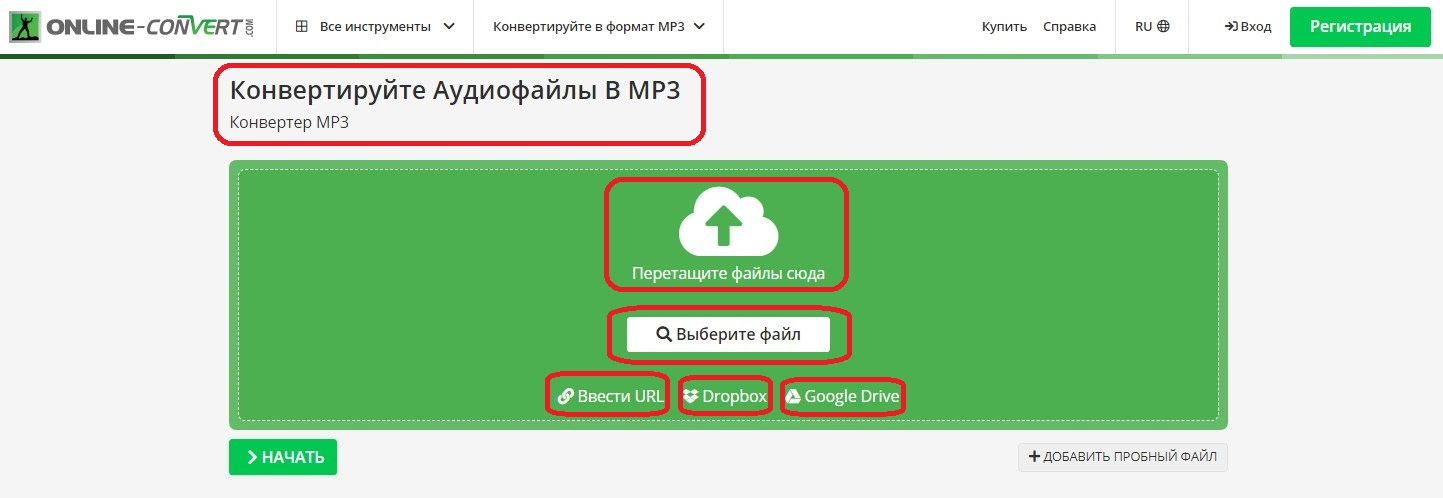
\includegraphics[width=0.8\textwidth]{img/cxp1.jpg}
\end{center}

В нашем примере мы видим, что есть 5 способов загрузить файл, который вам нужно конвертировать в mp3, на онлайн-сервис: найти в своем компьютере, взять с Dropbox, загрузить с Google-диска, загрузить с любого другого облачного хранилища или же просто перетащить в окошко загрузки, если папка с файлом уже открыта. Каждый сервис обозначен своим фирменным логотипом, а каждое действие – стандартным значком, обозначающим аналогичное действие на любом другом сайте.

По желанию пользователь может быстро ознакомиться с полным функционалом сайта, нажав меню «Все инструменты»:

\begin{center}
    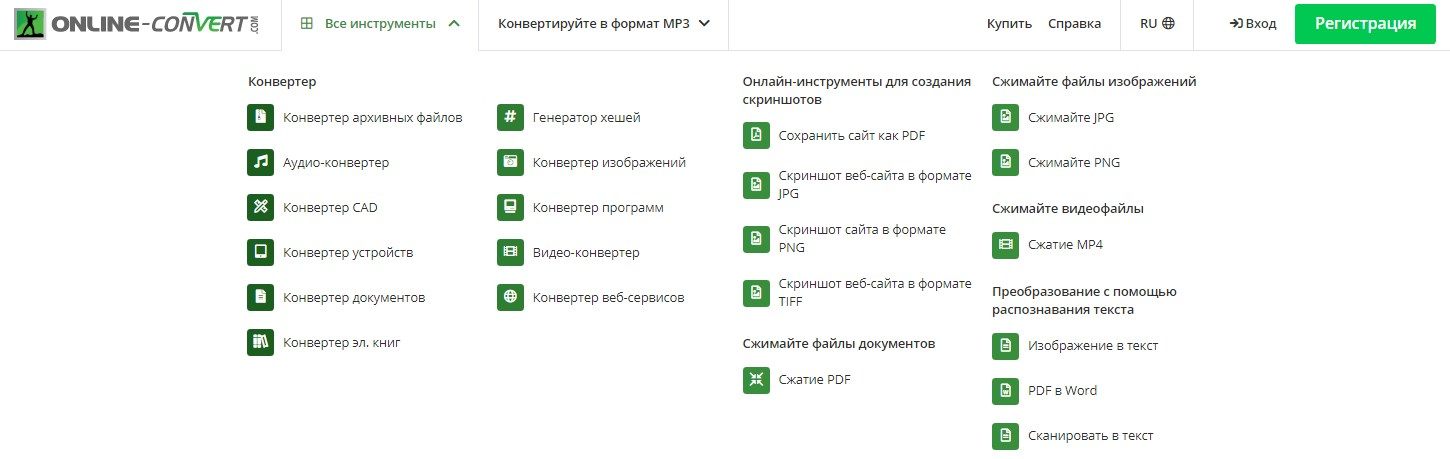
\includegraphics[width=0.8\textwidth]{img/cxp2.jpg}
\end{center}

В случае сомнений, нужен ли именно формат mp3 или какой-то другой, можно посмотреть все доступные форматы аудиофайлов:

\begin{center}
    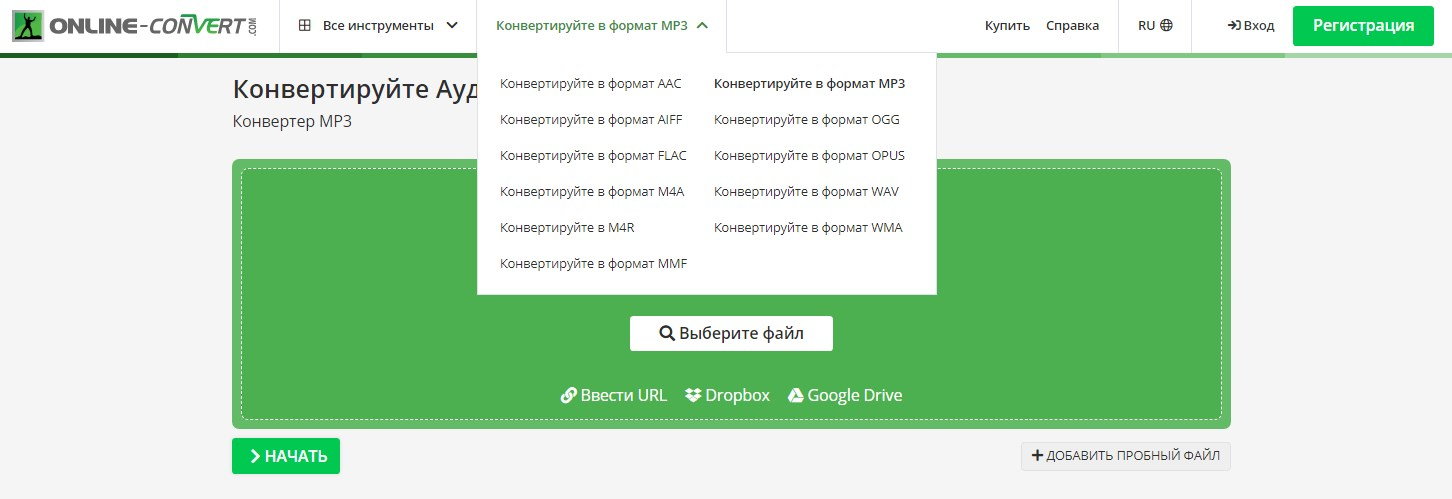
\includegraphics[width=0.8\textwidth]{img/cxp3.jpg}
\end{center}

Это пример соответствия ожиданиям пользователя, когда пользователь получает полный набор инструментов для своей дальнейшей работы и меньше чем за минуту знакомится с полным функционалом и возможностями сервиса.

\textbf{Видимость состояния системы}

Дизайн сайта, приложения, любого цифрового продукта должен быть построен так, чтобы пользователь всегда понимал, что сейчас происходит на сайте или в приложении, в какой части сайта или приложения он сейчас находится, насколько он приблизился к своей цели и каковы должны быть следующие действия.

Примером соблюдения принципа «видимости состояния системы» могут служить информационные уведомления наподобие «Выберите файл» и «Загрузка 50\%» на сайтах, где вы что-то загружаете или скачиваете. Это уведомления «Вы находитесь здесь» на сервисах с геолокацией, если вы разрешили доступ к данным о местоположении вашего гаджета. Такой интерфейс дает понимание, что делать дальше, и повышает доверие к цифровому продукту и бренду, предложившему этот продукт.

В рассмотренном выше примере, как только вы загрузили свой файл и нажали кнопку «Начать», появляется окошко с уведомлением, что «Ваш файл обрабатывается» и предупреждением «Не спешите. Страница результатов обновится автоматически»:

\begin{center}
    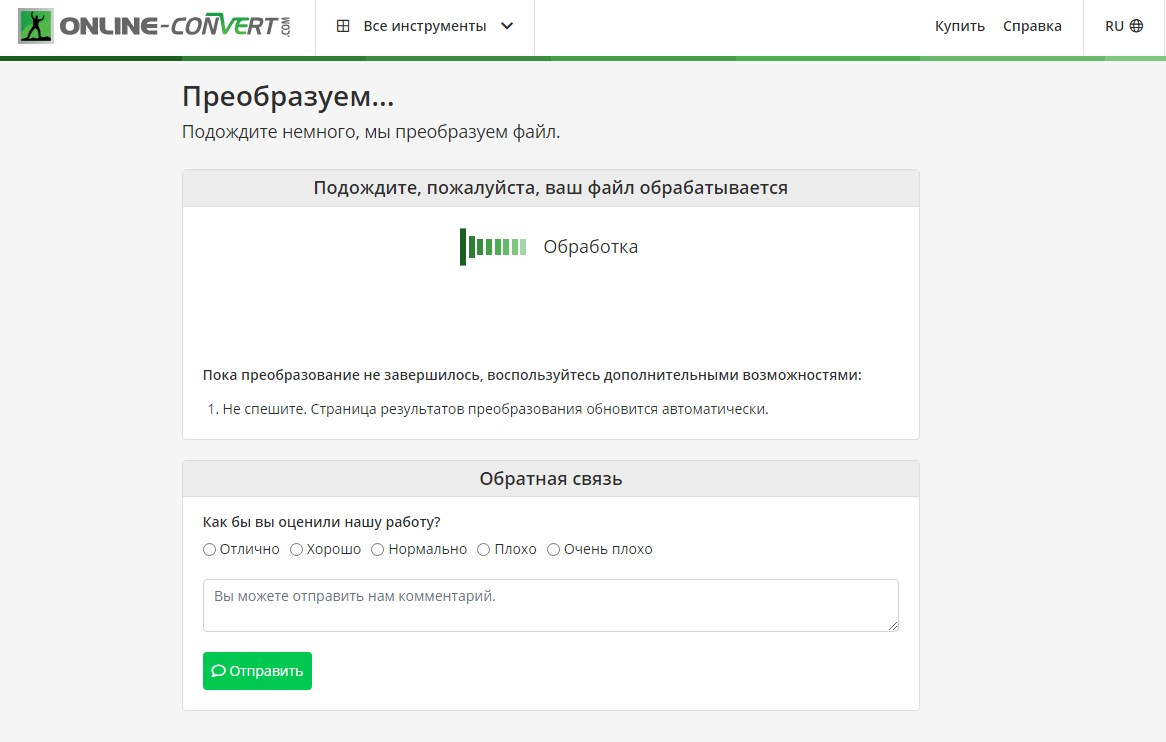
\includegraphics[width=0.8\textwidth]{img/cxp4.jpg}
\end{center}

Если вы уже обработали несколько файлов и вам скучно ждать, можно поставить оценку сервису или написать коротенький отзыв. Заметьте, сервис предоставляет такую возможность как бы «между делом», не забирая у пользователя его драгоценное время, когда он уже закончит работу с файлами, и не докучая потом сообщениями в духе «Оставьте отзыв».

\textbf{Пользовательский контроль и свобода}

Вероятность что-то не то нажать, не то загрузить или не то конвертировать есть всегда. У пользователя на каждом этапе должна быть возможность отменить действие либо удалить ошибочно загруженный или уже обработанный файл. В нашем примере сервис дает такую возможность с самого начала, как только пользователь загрузил свой файл на сайт, обозначив действие всем понятным значком в виде крестика и надписью «Удалить»:

\begin{center}
    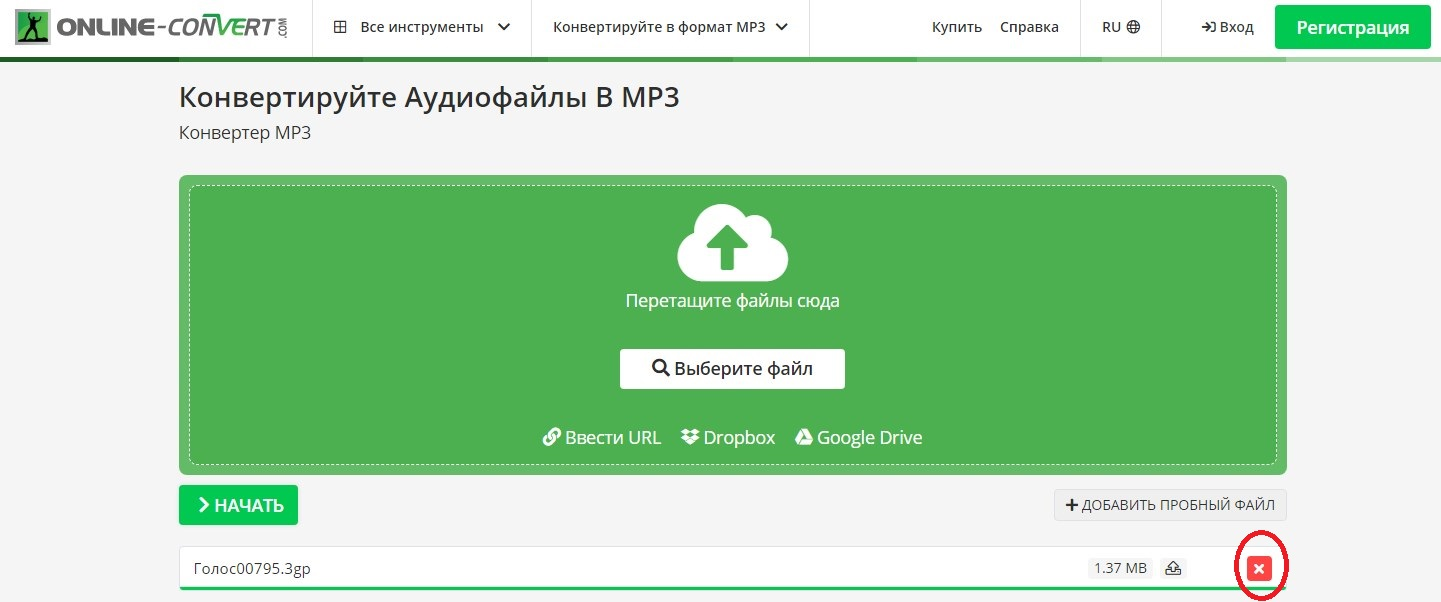
\includegraphics[width=0.8\textwidth]{img/cxp5.jpg}
\end{center}

Аналогичным образом можно поступить, если пользователь «спохватился» уже после того, как «отконвертил» файл. Помимо кнопок «Скачать» и «Загрузить в облако» есть кнопка «Удалить»:

\begin{center}
    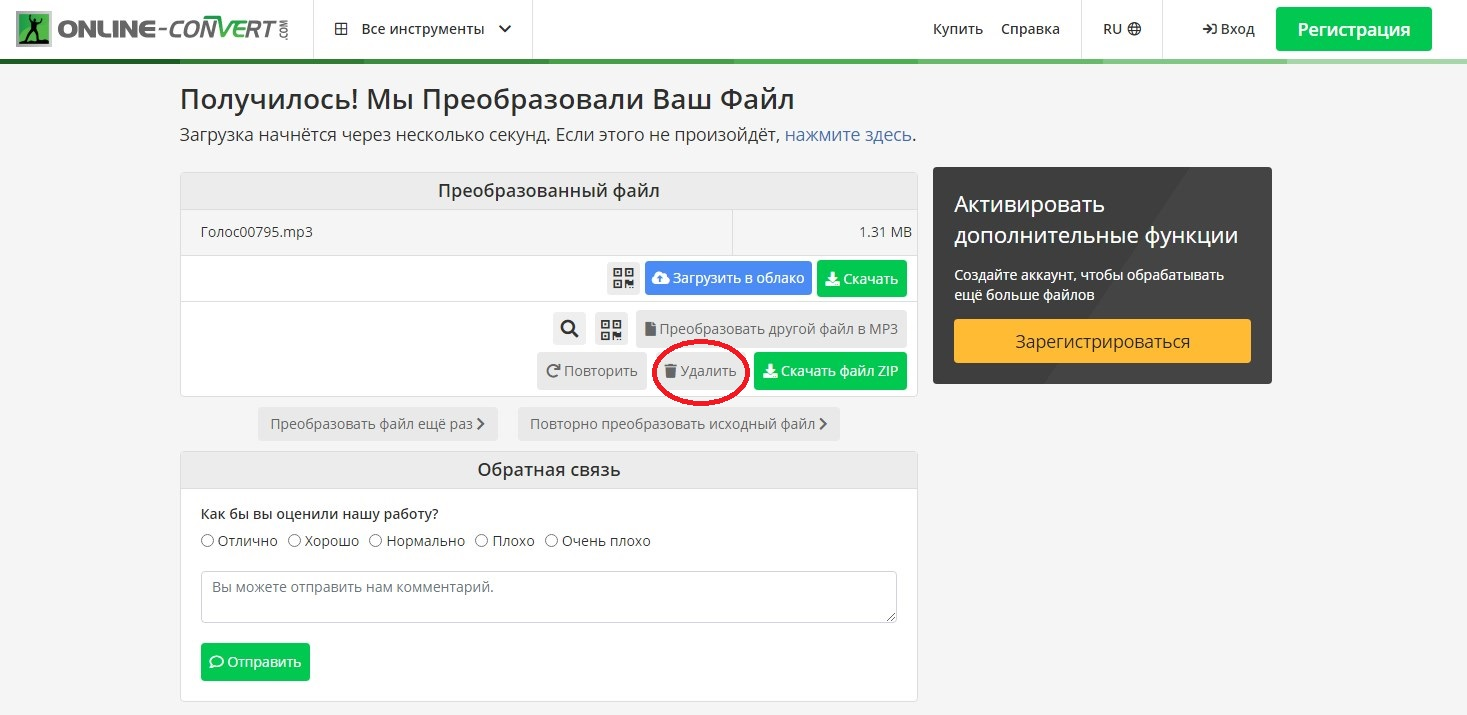
\includegraphics[width=0.8\textwidth]{img/cxp6.jpg}
\end{center}

Заметьте, что, если кнопки скачивания и загрузки выделены яркими броскими цветами, кнопка «Удалить» бледно-серая, дабы рука не тянулась к ней просто так, и пользователь не удалил готовый файл по ошибке.


\textbf{Предотвращение ошибок}

В продолжение темы следует сказать о предотвращении ошибок. Разумеется, никто не может застраховать пользователя от случайного нажатия кнопки и загрузки «не того» файла, однако обязанность разработчиков системы защитить пользователя от утечки данных и дать возможность в любой момент удалить данные не для широкого круга.

Если речь идет о более серьезных сервисах, связанных с денежными операциями, вариантом защиты может быть требование подтвердить ту или иную операцию (перевода денег, конвертации валюты и т.д.) Тут важно расставить приоритеты: сначала исключить серьезные ошибки, а затем минимизировать вероятность мелких неточностей.

Так, в нашем примере пользователь может не понять, что значить «Добавить пробный файл» и нажать эту кнопку из любопытства. Собственно, ничего страшного не происходит, и пользователь, убедившись, что это просто файл для демонстрации, как работает конвертер, может его сразу же удалить, не задерживаясь долго на странице и не отвлекаясь от своей основной задачи:

\begin{center}
    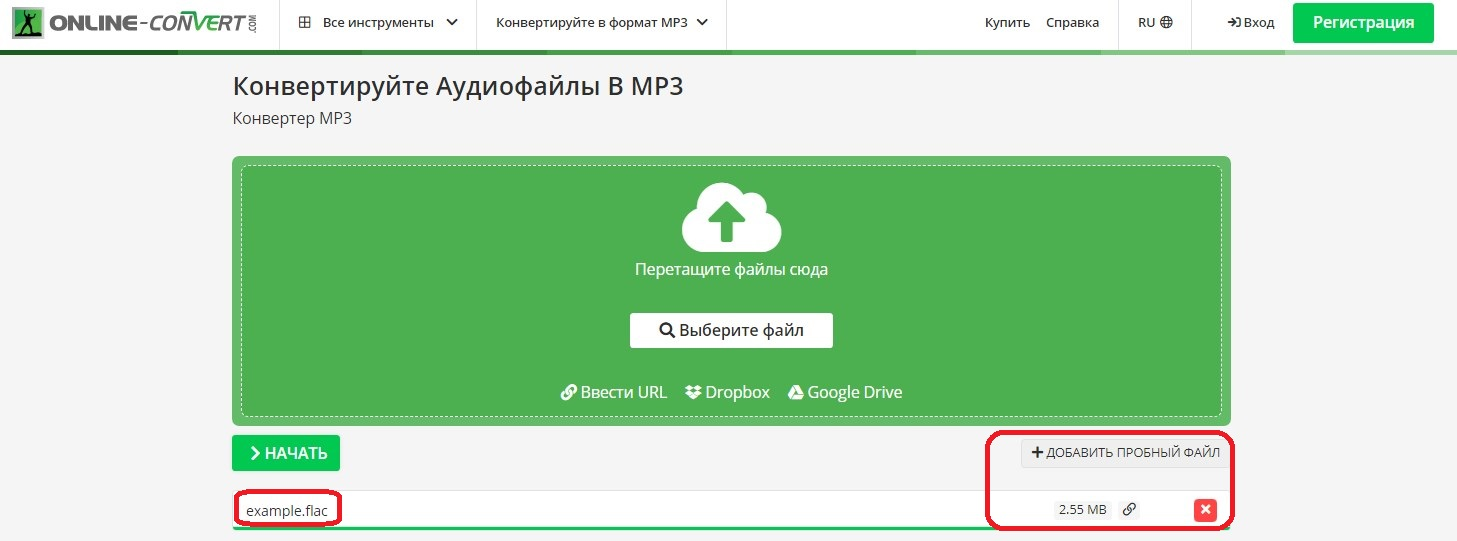
\includegraphics[width=0.8\textwidth]{img/cxp7.jpg}
\end{center}

Такие продуманные варианты предотвращения и исправления ошибок помогают «не выпадать» из стандартной последовательности действий.

\textbf{Последовательность и стандарты}

Любой продвинутый пользователь, вынужденно или добровольно проводящий онлайн по несколько часов в день, накапливает определенный опыт взаимодействия с цифровыми продуктами, а заодно и определенный массив ожиданий, как это взаимодействие должно происходить. Мы уже поговорили про соответствие ожиданиям пользователя с самого начала взаимодействия, но этого мало.

Соответствие стандартам и традиционной последовательности операций должна наблюдаться на всех этапах взаимодействия. Интерфейс может (и должен!) подсказывать возможные действия на шаг вперед, но ни в коем случае не опережать их и не сбивать с толку. В нашем случае вполне логично, что кнопка «Начать» появляется одновременно с кнопками загрузки файла. Так пользователю не нужно гадать, что будет дальше, когда он загрузит свой файл.

Аналогичным образом весь список возможных действий должен быть представлен по окончании каждого этапа. Например, после конвертации файла помимо кнопок «Скачать», «Загрузить» и «Удалить» появляется кнопка «Преобразовать следующий файл», чтобы пользователь не раздумывал, что ему делать дальше, если ему нужно конвертировать несколько файлов:


\begin{center}
    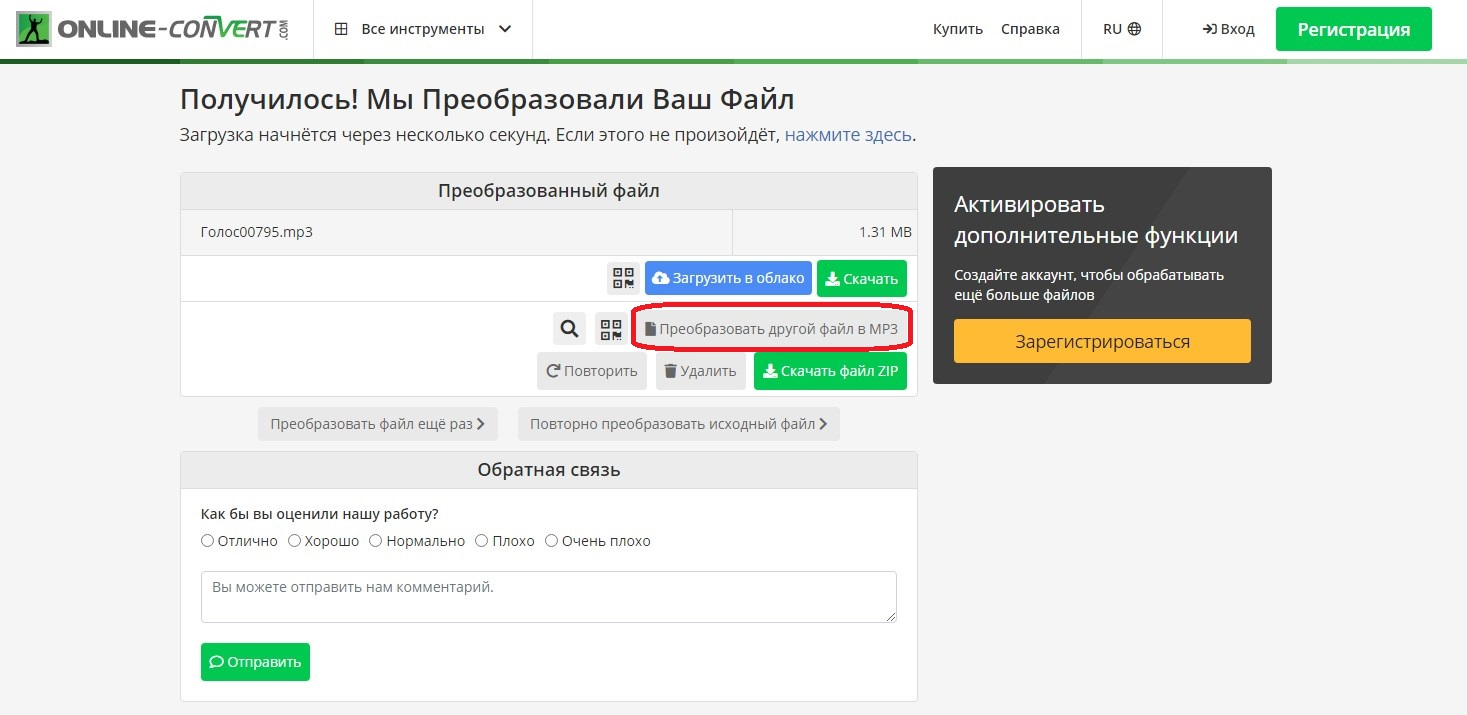
\includegraphics[width=0.8\textwidth]{img/cxp8.jpg}
\end{center}

Якоб Нильсен в своей статье отмечает, что неспособность сервиса поддерживать ожидаемую последовательность действий увеличивает когнитивную нагрузку на пользователей, когда это совершенно ни к чему [J. Nielsen, 2020]. Это примерно как стойка регистрации в отеле, что всегда расположена в холле. Если ее пришлось бы искать где-то через два коридора на другом этаже, это бы изрядно «напрягало» постояльцев отеля.

\textbf{Узнаваемость и напоминание}

Этот пункт «пересекается» с предыдущим. Чем более знакомым покажется пользователю интерфейс сайта, тем быстрее он на нем «освоится» и с тем большей вероятностью начнет заходить на этот сайт чаще. Особенно, если основной функционал сайта оправдает его ожидания.

Но данный пункт не только об этом. Он еще и том, чтобы снизить когнитивную нагрузку на пользователя даже в мелочах. Гипотетически юзер, конечно, должен помнить, какой именно файл он загрузил для конвертации минуту тому назад. Однако человека могут отвлечь какие-то дела, мысли, звонки. А если файлов много, можно просто сбиться со счета, потому как бесплатный сегмент сервиса позволяет конвертировать не более одного файла за один заход.

Именно поэтому основная информация об операции должна дублироваться на каждой странице каждого последующего шага. В нашем случае пользователь видит название загруженного файла как собственно при загрузке, так и после обработки:

\begin{center}
    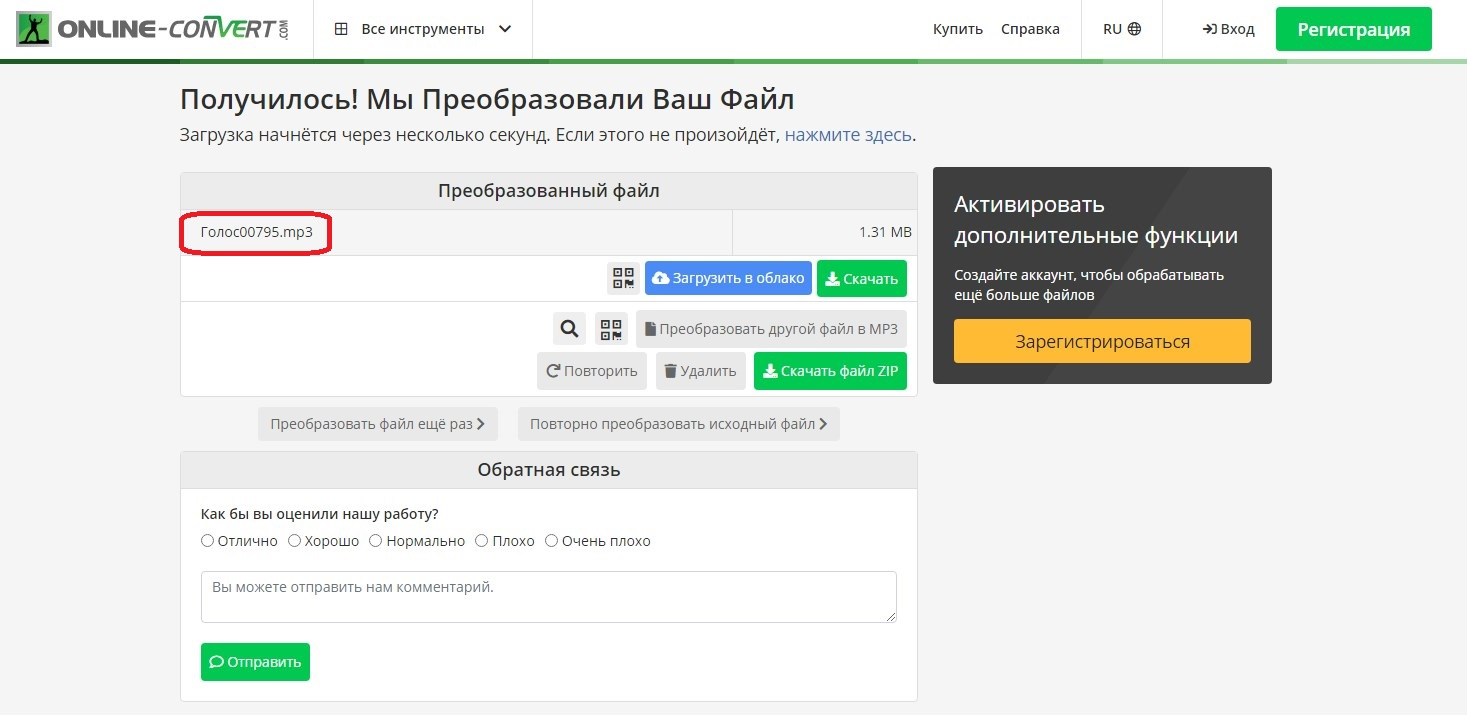
\includegraphics[width=0.8\textwidth]{img/cxp9.jpg}
\end{center}

К слову, это относится не только к оперативной информации, которая должна быть «на виду» и «под рукой». Аналогичным образом следует выстроить справочное сопровождение и помощь, предлагая ее в контексте возникшей проблемы, а не сразу весь мануал, 95\% из которого пользователю никогда не понадобится.


\textbf{Справочная информация}

Тем не менее, у пользователя должна быть возможность в любой момент найти ответ на любой свой вопрос, пусть даже пока у него никаких проблем не возникло. Раздел «Справка» должен быть на видном месте, лучше в верхнем меню, и структурирован на основные темы запросов пользователей:

\begin{center}
    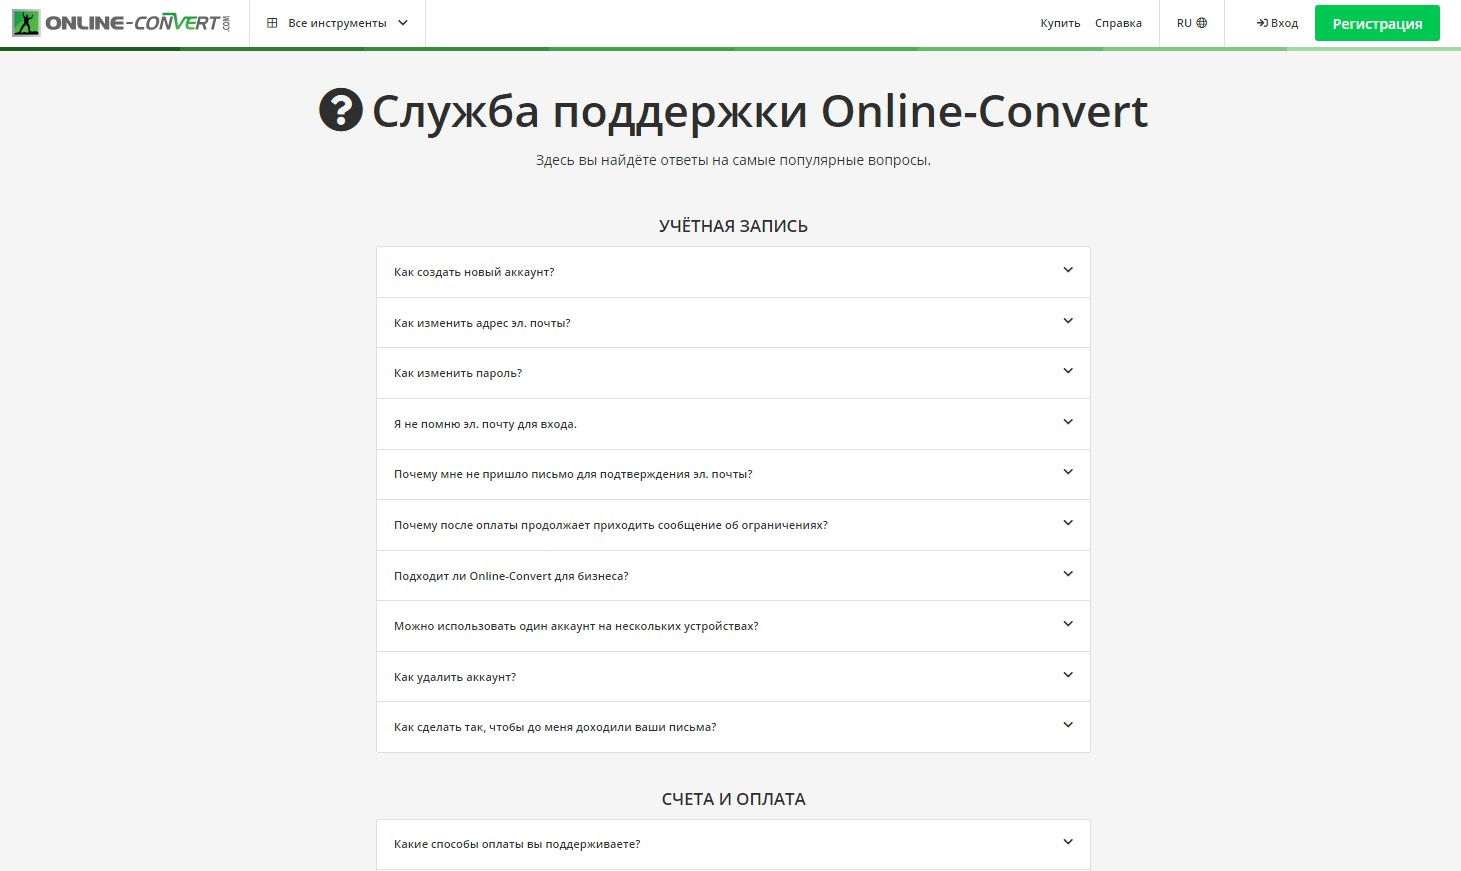
\includegraphics[width=0.8\textwidth]{img/cxp10.jpg}
\end{center}

Это, кстати, существенно разгрузит службу технической поддержки, потому что основной массив вопросов составляют одни и те же часто повторяющиеся проблемы, зачастую не имеющие никакого отношения собственно к сервису, а обусловленные человеческим фактором (забыл, не помню, не понял и т.д.). Разумеется, такого рода вопросы тоже должны быть обеспечены ответами.

\textbf{Гибкость использования}

Про индивидуальный подход слышали все, но не все разработчики вняли. Так, гибкость процессов – это «наше все». Не нужно «грузить» человека, которому нужно конвертировать один файл, информацией о годовой подписке. Эту информацию нужно предоставить только зарегистрированным пользователям.

Следует внятно написать, что именно даст регистрация на сайте и зачем она в принципе нужна. Например, для того, чтобы за один заход обрабатывать больше файлов, а не один, как в бесплатной версии:

\begin{center}
    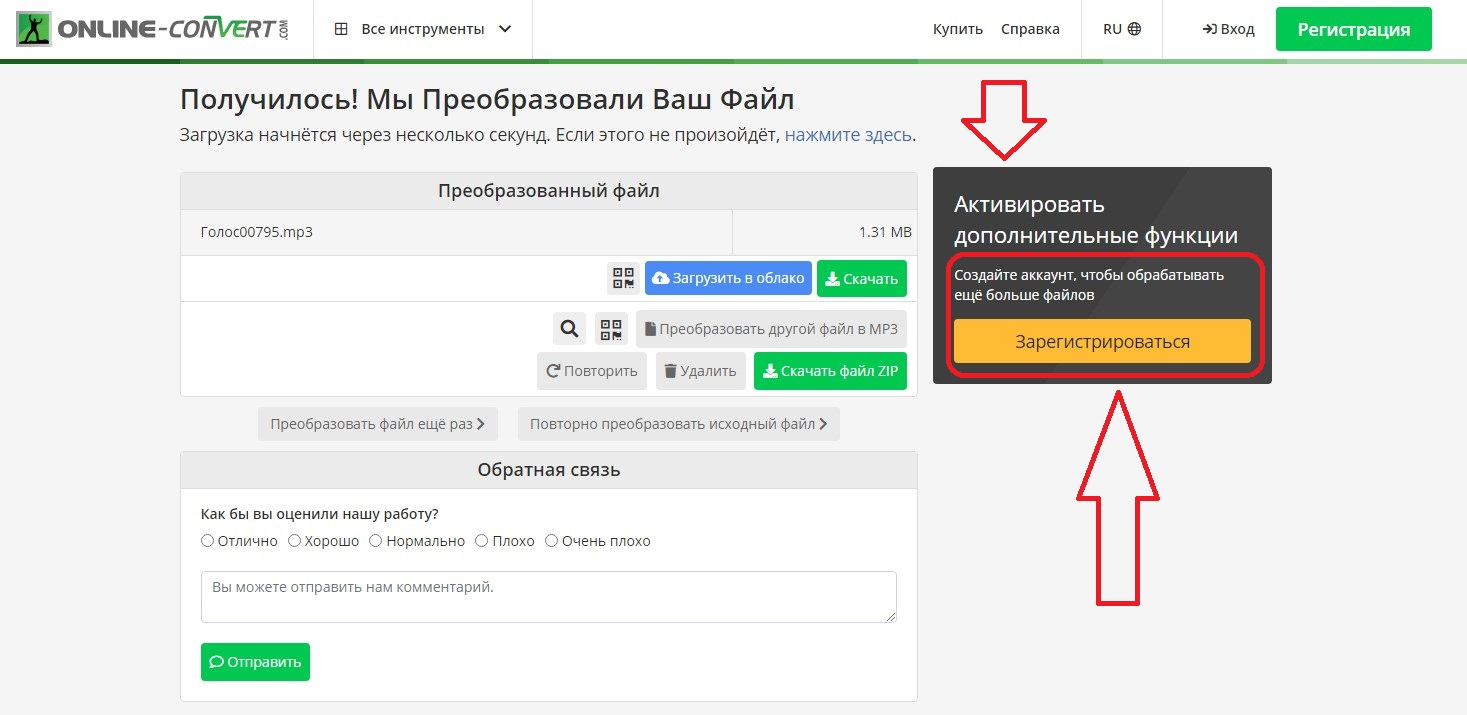
\includegraphics[width=0.8\textwidth]{img/cxp11.jpg}
\end{center}

Такая прозрачность избавит пользователя от возможных разочарований, а владельцев сайта – от негативных отзывов недовольных посетителей, потративших время на регистрацию непонятно зачем.

\textbf{Минимализм в дизайне}

Данный пункт связан со всеми предыдущими пунктами сразу. Если держать в фокусе только актуальную необходимую информацию, текущее действие и следующие возможные шаги, нет никакой необходимости перегружать сайт лишней информацией, картинками, элементами дизайна. Вот и не перегружайте.

Выражаясь научным языком, каждая дополнительная единица информации в интерфейсе конкурирует с другими единицами информации, в результате чего снижается относительная видимость каждой единицы информации [J. Nielsen, 2020].


\textbf{Помощь пользователям}

Про помощь пользователям в обращении с интерфейсом и использовании сервиса мы поговорили достаточно подробно. Однако могут возникнуть не зависящие от владельца сайта обстоятельства, мешающие воспользоваться сервисом. Например, прервется онлайн-соединение.

Сообщить об этом нужно простым и понятным языком: «Проверьте подключение к Интернету». Лучше не писать «Нет Интернета», потому что так пользователю может быть не совсем понятно, у кого именно нет интернет-соединения: у него или у вас.

Это и есть 10 эвристик юзабилити для дизайна пользовательского интерфейса. К слову, первоначальный вариант статьи Якоб Нильсен написал в далеком 1994 году, а в 2020 году только дополнил и расширил статью с учетом актуальной информации. Тем не менее, все базовые постулаты остались прежними. Как метко заметил автор, если что-то работает и остается неизменным на протяжении почти 30 лет, весьма вероятно, что это будет актуально еще достаточно долго.

Так что все эти рекомендации лучше соблюдать. В противном случае можно наделать много досадных ошибок, которые будут снижать конверсию и отпугивать пользователей.

\textbf{Основные ошибки в дизайне по Нильсену}

Какие ошибки можно совершить, проектируя дизайн интерфейса? Подробно об этом рассказал сам Якоб Нильсен в своей работе Top 10 Mistakes in Web Design («Топ-10 ошибок в веб-дизайне») [J. Nielsen, 2011]. Тут очень много самоочевидного, но почему-то все еще не воспринимаемого дизайнерами, разработчиками и заказчиками цифровых продуктов. Поэтому ограничимся просто списком с короткими пояснениями.

Топ-10 ошибок в веб-дизайне:

\begin{enumerate}
    \item Неудобный поиск – когда невозможно ничего найти, когда результат поиска нерелевантен запросу, когда на короткий внятный вопрос «выпадает» мануал на 150 страниц и т.д.
    \item PDF-файлы для онлайн-чтения – они оптимизированы под формат А4, а не под размер экрана, из-за чего возникает множество неудобств, начиная от мелкого шрифта и заканчивая неудобной прокруткой.
    \item Ранее просмотренные пользователем ссылки не меняют цвет – в итоге легко запутаться, особенно, если на сайте много контента.
    \item Нечитаемый текст – отсутствие разбивки на абзацы, слишком длинные абзацы, отсутствие разделов, подразделов и какой-то внятной структуры, избыток узкоспециальных терминов и профессионального жаргона.
    \item Фиксированный размер шрифта – не подходит для людей с не очень хорошим зрением, не желающим носить очки.
    \item Сходство с рекламой – если какой-либо раздел сайта похож на рекламу, его с высокой долей вероятности просто не станут изучать.
    \item Появление новых окон в браузере – это примерно как с рекламой, поэтому даже очень нужное окно чата с ботом лучше предлагать не сразу, а хотя бы через полминуты, чтобы пользователь успел «осмотреться» на сайте.
    \item Вопросы без ответов – когда ответ нельзя найти ни через поиск, ни через бот, ни через раздел «Справка», ни собственно в разделе сайта. Либо когда отсутствует информация, которая должна наличествовать по умолчанию. Например, цена товара в интернет-магазине.
    \item Нарушение общепринятых правил дизайна – меню должно быть вверху, строка поиска тоже вверху, кнопка «В корзину» вверху справа и т.д. Если такие общепонятные вещи приходится искать непонятно где, пользователь чаще всего просто уходит с сайта.
    \item Заголовки страниц не оптимизированы под поисковые системы – есть риск, что в этом случае даже очень ценная информация так и не попадет к пользователю. «Добро пожаловать» и «Внимание» не подходят, равно как и «Интересное предложение», «Акция», «Скидка» без пояснений, к чему это все относится.
\end{enumerate}

Небольшая подсказка к последнему пункту: заголовок страницы содержится внутри HTML-тега и почти всегда используется в качестве кликабельного заголовка среди результатов выдачи поисковых систем (SERP). Это для тех, кто хочет заняться оптимизацией сайта лично.

Итак, мы достаточно подробно рассмотрели все нюансы закона Якоба Нильсена. Осталось только им безоговорочно следовать… Или нет?.. Некоторые считают, что нет.


\textbf{Нюансы интерпретации закона Якоба Нильсена}

Сразу скажем, откуда взялся скептицизм в отношении закона Якоба Нильсена. И, кстати, не только в отношении него. Есть такая интересная статья «Ошибки в интерпретации UX законов: неверно понятые правила UX» [Р. Наджафов, 2022]. Тут, правда, больше не об ошибках, а о том, что все хорошо в меру.

Закон Якоба Нильсена частенько интерпретируют как призыв к примитивизму, отказу от эксперимента и креатива, использованию готовых шаблонов на все случаи жизни, потому что пользователям нужен узнаваемый дизайн, интуитивно понятный функционал и т.д. Имел ли это в виду сам Якоб Нильсен?

Вряд ли, потому что удобная навигация по сайту и креативные картинки к статьям в блоге никоим образом не исключают друг друга. Кроме того, вполне можно как-то нешаблонно сказать пользователю «Спасибо» за то, что он воспользовался вашим сервисом, когда он уже получит желаемый результат и точно не отвлечется от процесса на картинку с котиком, вручающим ему букет цветов.

Кроме того, новые впечатления поднимают настроение, а за хорошим настроением пользователь всегда охотно вернется на понравившийся сайт. Поэтому повторимся, что все хорошо в меру, во всем нужен баланс, а шаблоны и стандарты нужны исключительно для обеспечения удобства пользования.



\newpage

\chapter{Кино}

\section{Кино}
\textbf{Возникновение\footnote{возникновение: emergence}.}
В конце XIX века движение предмета наконец-то \explain{удал\'{о}сь}{удаваться/удаться: to manage} \explain{перенести}{переносить/перенести: to transfer} на экран. Вскоре после этого, кино начало набирать популярность. Первые фильмы были очень короткие, продолжительностью около 1-ого минуты. Они были черно-белыми и без звука. \explain{Спуст\'{я}}{later; after; e.g., спустя три дня} несколько лет продолжительность фильма уже составляла 15-20 минут.

\textbf{Виды фильмов.}
Существует несколько видов фильмов, такие как короткометражное кино, документальные и художественные фильмы.
Короткометражное кино является \explain{отд\'{е}льным}{отд\'{е}льный: separate} жанром. Нужно быть профессионалом, чтобы передать целый ряд чувств за короткий промежуток времени. Продолжительность таких фильмов обычно не \explain{превышает}{превышать: to exceed} 15-20 минут.

В основе документальных фильмов лежат реальные истории и факты. Обычно, это фильмы об исторических \explain{событиях}{событие: event}, знаменитых людях и т.д.
Образовательные фильмы также относятся к этой категории.

Художественные фильмы --- это фильмы, в которых актёры играют определённую роль. Художественные фильмы бывают разного жанра: мелодрамы, комедии, триллеры и другие.

\textbf{Российское кино.}
Стремительное \explain{развитие}{development} российского кино началось в XXI веке. Многие фильмы \explain{напр\'{а}влены}{short form of направленный (adj.): directed} на массового зрителя и, \explain{в большинстве своем}{largely}, развлекательные. Кроме того, \explain{выпускается}{выпускаться/выпуститься: to be released} большое количество фильмов высокого качества. Российский кинематограф известен своими талантливыми режиссёрами, такими как Никита Михалков, Федор Бондарчук, Тимур Бекмамбетов и некоторыми другими.

\textbf{Голливуд.}
Голливуд является самым популярным местом по \explain{производству}{производство: production} фильмов в мире. Ежегодно там \explain{создаются}{создаваться/создаться: to be created} тысячи фильмов. Голливудские фильмы полны спецэффектов, которые привлекают миллионы людей в кинотеатры.

\section{Человечество решает умереть}
\textit{Ярослав Забалуев}\\
\url{https://lenta.ru/articles/2021/12/25/dontlookup/}

{\it Вышла комедия про дураков и апокалипсис с Ди Каприо, Стрип и Бланшетт. Зачем ее смотреть?}

\textit{На Netflix вышла новая комедия известного «Игрой на понижение» Адама Маккея «Не смотрите наверх» --- хвастающая, возможно, самым звездным за последнее время актерским составом. «Лента.ру» рассказывает, почему фильм о конце света с Леонардо Ди Каприо в главной роли --- идеальное кино для конца этого странного года.}

Астрономы Рэндалл Минди (Леонардо Ди Каприо) и Кейт Дибиаски (Дженнифер Лоуренс) обнаруживают, что к Земле мчится комета диаметром в десяток километров. Столкновение с планетой может привести к полному исчезновению не только человеческой, но и вообще всякой жизни. Рэндалл и Кейт грузятся в самолет и отправляются в Вашингтон, чтобы обсудить планы спасения Земли с высочайшими государственными чинами. Однако выясняется, что президент Дженни Орлин (Мэрил Стрип) куда больше увлечена живописным курением и секстингом с каким-то региональным отморозком. Главой администрации работает ее сын Джейсон (Джона Хилл), который в свою очередь в основном хвастается новой татуировкой дракона и упивается властью ходить на работу упоротым.

Минди и Дибиаски пытаются добиться огласки, выступив в популярном телешоу, однако Кейт заслуживает лишь волну мемов в интернете, а Рэндалл --- недвусмысленные знаки внимания ведущей (Кейт Бланшетт), которую возбуждает, что скоро мы все умрем. В какой-то момент правительство США все же снарядит спасательную экспедицию, но сразу после старта развернет ракеты, поскольку на сцену выйдет Питер Ишервелл (Марк Рейланс) --- визионер, объясняющий, что из столкновения с кометой тоже в теории можно извлечь пользу.

Фильмы и сериалы-катастрофы прошлого и нынешнего годов дали повод вновь заговорить о сверхъестественном чутье художников, прозревающих будущее без всяких на то логических объяснений. Вот и разработка «Не смотрите наверх» началась еще во вполне безмятежном ноябре 2019-го. Впрочем, никакой безмятежностью, разумеется, и не пахло --- Дональд Трамп вовсю собирался на второй срок, а Америка все глубже погружалась в депрессию, лекарство от которой так и не придумали до сих пор. Тем не менее за без малого полтора года, которые занял путь картины к зрителю, в мире изменилось слишком многое, создав для «Не смотрите наверх» уникальный и куда более подходящий случаю контекст.

В сверхъестественной проницательности в данном случае стоит обвинять сценариста и режиссера Адама Маккея. Это автор удивительной судьбы. Шесть лет назад он не пожелал сидеть в комедийном жанровом гетто и после дилогии про Рона Бургугди («Телеведущий») бросился покорять новые территории. В итоге его «Игра на понижение» стала одним из самых остроумных фильмов про кризис 2008-го года и принесла Маккею «Оскар» за лучший адаптированный сценарий. Через три года, в 2018-м, Адам решил развить успех и одновременно взвинтить ставки --- его «Власть» имела в своем центре ни много ни мало бывшего вице-президента Дика Чейни. Сатирический байопик абсолютного зла (именно такова трактовка Маккея) был воспринят чуть менее однозначно, несмотря на очередной актерский подвиг Кристиана Бейла. И вот в следующем своем проекте режиссер совместил едкий социальный комментарий с внешне легкомысленным задором своих ранних комедий.

\begin{fancyquotes}
    Кажется, что фильмы про летящие к Земле кометы вышли из моды на рубеже тысячелетий --- нулевые показали, что над нами летают штуки и пострашнее
\end{fancyquotes}

Последней из больших голливудских картин на тему, конечно, был пропагандистский шедевр Майкла Бэя «Армагеддон». Это было кино, где все важные вещи говорили на фоне развевающегося звездно-полосатого флага, а Брюс Уиллис, наконец, смог погибнуть --- но только под песню Aerosmith. Самым ярким послесловием к этому сюжету стала «Меланхолия» Ларса фон Триера, который с явным удовольствием разнес-таки нашу планету в труху. «Не смотрите наверх» отсылает к этим двум фильмам вполне прямолинейно. «Армагеддон» спародирован целыми фрагментами, а Уиллиса заменил Рон Перлман --- и так даже смешнее. С «Меланхолией» у Маккея значительно более нежные отношения. Пародиями тут не пахнет, скорее уж речь идет о трепетном оммаже --- при желании героинь Лоуренс и Бланшетт можно без особых поправок поместить в триеровский контекст.

Однако прямые и не очень аллюзии в данном случае отнюдь не самоцель. Маккей использует энергию предшественников, чтобы напитать ей совершенно авторское высказывание, сделанное, как водится, в сатирическом ключе. Режиссер владеет этим сложнейшим на самом деле жанром виртуозно и в «Не смотрите наверх» явно упивается возможностью не заботиться об исторической достоверности. На орехи тут достается абсолютно всем: озверевшим от самодовольства селебрити политикам, мямлям-ученым, не способным разговаривать человеческим языком, дурящим народ визионерам со своими дурацкими смартфонами… Перечислять мишени Маккея можно долго и с удовольствием, благо режиссер не придерживается более или менее никакой конкретной позиции --- просто стреляет во все, что видит.

За без малого два с половиной часа от такого потока желчи и презрения можно было бы устать, но фокус в том, что «Не смотрите наверх» этих потоков на зрителя, в общем, не льет. Остроумие наблюдений и сарказм авторских комментариев здесь уравновешен удивительно человечной интонацией. У Маккея с его врожденной язвительностью и острым глазом нет ответов на вопрос «что делать?» За происходящим на экране балаганом сквозит растерянность умного человека, вынужденного, как обычно, пытаться хоть как-то достучаться до идиотов. Это, пожалуй, и правда самая адекватная эмоция в мире, где ученый, сообщающий в ток-шоу о гибели человечества, добивается лишь статуса «астронома, которого я бы трахнула». Зато об этом мире можно снять фильм, который под конец очередного безумного года дарит не столько депрессию, сколько радость и умиротворение. Если мы все равно скоро умрем, то нет ни одной причины отказываться от праздничного ужина.

Фильм «Не смотрите наверх» (Don't Look Up) вышел на Netflix 24 декабря


\chapter{Талант}
\input{topic/39_smoking_prohibition.tex}
\input{topic/40_curios.tex}
\chapter{Мода}

\section{Как мода влияет на нашу жизнь?}

\textit{Источник: \url{https://absurdu.net/fashion/kak-moda-vliyaet-na-nashu-zhizn.html}}

С развитием современных технологий, соцсетей и рекламы большинство из нас осознает, что в той или иной мере мы таки поддаемся определенным трендам и модным тенденциям. И все же, существует немало тех, кто категорически не согласен с этим утверждением. Такие люди утверждают, будто бы мода никоем образом не влияет на их жизнь и, тем более, на поведение. Но так ли это на самом деле? Давайте разбираться!

\textbf{Отражает мировые события и общий настрой людей}

Ни для кого не секрет, что мода всегда отражает культурные, социальные, политические, экономические и религиозные аспекты общества. Если в мире происходит что-то масштабное, это в любом случае тем или иным образом повлияет на fashion-индустрию. Так формируются определенные тренды. Яркое доказательство этому – тенденции 2021 года. Психологи говорят о том, что при возникновении неприятных событий человек нуждается в том, что могло бы положительным образом повлиять на его настроение. Этот принцип находит свое отражение и в модной индустрии. После пандемии и локдауна многие чувствуют усталость и подавленность. Дизайнеры, ощущая потребности своих клиентов, начали создавать более комфортную, но в то же время креативную одежду: мода понемногу отходит от нейтральных оттенков и непрактичных вещей, наоборот, повседневные предметы гардероба становятся более удобными, а палитра цветов гораздо ярче. Насыщенные цвета радуги положительным образом влияют на наше самоощущение и восприятие мира, а интересные фасоны, асимметрия или архитектурный крой в одежде смотрятся нарядно и элегантно, что способствует ощущению воодушевленности и праздничного настроения.

К интересным выводам пришли также те, кто занимается изучением истории fashion-индустрии. После масштабных войн или экономических кризисов одежда становилась все более откровенной. Фасоны прилегали к телу, подолы юбок и платьев укорачивались. С одной стороны, это было связано с практичностью, а с другой – с банальной нехваткой материалов. Из-за тяжелого положения в такие времена люди просто не могли тратить по 40 метров ткани на одно платье!
То же самое можно сказать и про сферу религии и морали. Все знают, что в мусульманских странах девушки не могут носить одежду, которая бы открывала их шею, запястья или щиколотки. Поэтому мода в таких государствах обычно гораздо более консервативная, но все же поддается изменениям. Тем более, что под хиджабом или паранджей женщина может носить то, что нравится ей, если это соответствует принципам одежды, записанным в Коране. Кроме того, в большинстве случаев они не ограничены в выборе аксессуаров. Так, например, во всемирно известном торговом центре Dubai Mall в ОАЭ, куда съезжаются люди из всех уголков мира, довольно часто можно встретить пару, в которой супруга идет в лодочках от любимого люксового бренда, а руках у нее оригинальная сумка Chanel или Dior.

\textbf{Продвигает инклюзивность, меняет представление о красоте}

Конечно, представление о «красоте» очень субъективное, но, тем не менее, наше восприятие этого абстрактного понятия в огромной мере зависит именно от «канонов» fashion-индустрии. До 70-80-х прошлого века люди не сильно обращали внимание, на то, как выглядит их тело. Но с популяризацией спорта и развитием некоторых его видов в моду приходит «культ тела», подразумевающий подтянутую спортивную фигуру не только у мужчин, но также и у женщин. Вспомните также, как менялось представление об идеальных модельных параметрах: в 2000-е годы большинство представительниц этой профессии имели явно нездоровый вид, что чаще всего было следствием анорексии. Со временем, когда суровый fashion-мир наконец-то переосмыслил понятие красоты и здоровья, на подиумы стали выходить модели плюс-сайз. То же самое касается и темнокожих девушек: еще в конце прошлого века для большинства из них принять участие в показе или появиться на обложке глянца казалось недостижимой целью, а сегодня вопрос происхождения не является препятствием при построении карьеры. Если говорить об особенностях, как, например, кожа супермодели Винни Харлоу или страбизм (косоглазие) Брунетт Моффи, все больше людей также перестают обращать на это внимание.

Выпускники Лондонского колледжа моды Джудит Ахумба-Велленстайн, Сьюзан Джин и Пак Лунчиу, которые создали онлайн-журнал Hajinsky, посвященный фэшн-психологии, изучив то, какое воздействие мода имеет на жизнь большинства людей, пришли к следующему выводу:

\begin{fancyquotes}
    «Официальная одежда положительно влияет на абстрактное мышление человека, которое связано с такими действиями, как, например, экономия денег. Кроме того, наука показала, как бренды могут улучшить жизнь общества, сделав одежду инклюзивной. Исследования показали, что люди с ограниченными физическими возможностями часто для удобства носят спортивные костюмы и поэтому подвергаются двойной дискриминации — во-первых, из-за своей физических особенностей, во-вторых, из-за своей одежды. Бренды, принимающие это во внимание, могут в корне изменить жизнь человека».
\end{fancyquotes}

\textbf{Исполняет роль идентификатора личности}

Мода также помогает нам больше понять других и служит неким идентификатором. Например, по национальному костюму мы можем догадаться, из какой страны человек, общий внешний вид иногда указывает на род деятельности, а характерная манера сочетать вещи может служить неким маркером «творчества», «вкуса» и т.д. Те же, кто все еще категорически отказываются принимать факт влияния моды на их жизнь, не могут отрицать того, что в современном мире просто нельзя избежать ситуаций, когда мы должны выглядеть определенным образом. Представьте, что вас пригласили на свадьбу, на торжественный ужин в дорогой ресторан или же вы идете на собеседование в крупное финансовое учреждение с наличием определенного дресс-кода. Для такой ситуации вы вряд ли наденете джинсы. Для подобных случаев существует различные наряды, в том числе классический деловой костюм, который так же пришел в нашу жизнь под влиянием определенных тенденций. Нельзя отрицать тот факт, что внешний вид человека также сказывается на том, как другие воспринимают его. Именно по этой причине мы часто задумываемся о том, какую одежду подбирать не только под определенную ситуацию, но даже под сам круг общения. Наше естественное желание нравиться способствует тому, что время от времени мы обновляем свой гардероб и добавляем туда красивые (которые соответствуют нашему субъективному вкусу) предметы одежды и аксессуаров.

\begin{fancyquotes}
    «Реальность такова, что мода стала частью нашей повседневной жизни. Она связана с политикой и может вызвать социальные перемеФормирует сознаниены. Мода также влияет на наши отношения друг с другом, наше поведение, она может улучшить нашу жизнь, помогая с самоидентификацией»,- заявили вышеупомянутые основатели журнала Hajinsky.
\end{fancyquotes}

\textbf{Формирует сознание}

И это касается даже тех, кто никогда не следит за ней. Если все начинают носить оверсайз, со временем при покупке новой футболки вы также сделаете выбор в пользу прямого или более свободного фасона. Кроме того, это отражается и в количестве покупаемых предметов. Сейчас большинство людей приобретают намного больше одежды, обуви и аксессуаров, чем это было еще 30 лет назад.

\begin{fancyquotes}
    «При выборе гардероба важно ориентироваться на свои ценности и цели. При этом человек не может существовать в полном отрыве от общества. В этом смысле, если „психология моды“ про гармонизацию запросов общества и внутренних процессов человека, то это может повысить качество его жизни». – Говорит психолог Александра Меньшикова.
\end{fancyquotes}

Также нельзя забывать, что мода – это не только об одежде. Поэтому если вы не следуете трендам при формировании своего гардероба, это не значит, что вы не изучите последние тенденции, когда, например, будете делать ремонт в квартире. То же самое касается приобретения новой техники, автомобиля или даже посуды на кухню.

Хотите вы того или нет, мода в любом случае влияет на ваш выбор повседневных образов, домашней обстановки и даже места для отдыха. И это нельзя определить как «хорошо» или «плохо» — каждый оценивает по-своему. Остается лишь принять тот факт, что мода в большой степени влияет на разные сферы нашей жизни, а вот активно следовать новым тенденциям, принимать их или всеми силами пытаться убежать от них – личное дело каждого. Но, согласитесь, знание — сила. Осознанность поможет вам разумно подходить к вопросу трендов и тенденций, чтобы умело использовать этот инструмент для достижения своих целей. Актуальный и стильный внешний вид еще никому не помешал.
\chapter{Транспорт и дорожное движение}

\section{Дорожной концессии нужен сигнал}

\textit{На какие проекты надо делать ставку при строительстве трасс с привлечением частного капитала}

% https://www.vedomosti.ru/industry/infrastructure_development/articles/2023/03/29/968707-dorozhnoi-kontsessii-nuzhen-signal
\textit{Источник: \url{https://www.vedomosti.ru/industry/infrastructure_development}}

\textit{Олеся Ошанина}

Концессионные соглашения в дорожном строительстве давно уже стали классикой, поскольку реализация столь капиталоемких проектов возможна лишь с государственной поддержкой. В нашей стране строительство дорог регионального значения является наиболее перспективной формой государственно-частного партнерства (ГЧП), однако отсутствие четких сигналов от федеральных властей о том, какие проекты являются приоритетными, является препятствием для активного строительства дорог с привлечением частного капитала.

В условиях современной экономики развитие партнерских отношений государства и частного сектора считается оптимальным способом повышения эффективности использования государственной собственности. Одной из важнейших форм ГЧП являются концессии. Их главным плюсом является возможность привлечения внебюджетных инвестиций и ресурсов в государственный сектор, в то время как концессионер получает возможность эксплуатировать объект и получать доход в свою пользу.

\textbf{Дорогие дороги: объединение капиталов}

ГЧП и концессии в автодорожном строительстве – это мировая классика, указывает директор группы по привлечению финансирования Kept Сергей Игнатущенко. «Инвестор строит дорогу, зная, что 30 лет ему потом эту дорогу содержать и ремонтировать, поэтому построит качественно, – указывает эксперт. – Более того, считается, что дорожные концессии на горизонте жизненного цикла проекта дешевле государственного заказа, поскольку инвестор берет на себя риски уложиться в смету и риски эксплуатации – именно инвестор умеет такими рисками профессионально управлять». Именно в дорогах наиболее просто спрогнозировать и оценить экономический эффект для всех участников проекта, при этом не имеет значения – взимается плата за провоз груза или за проезд автомобиля, соглашается генеральный директор ГЧП.РФ Виталий Нефедов.

\begin{fancyquotes}
    \textbf{ГЧП – цифры и факты.} Согласно аналитическому обзору Национального центра ГЧП, в России по состоянию на конец 2022 г. было 3724 проекта ГЧП, среди которых 2720 были в сфере коммунально-энергетической инфраструктуры, 652 – социальной инфраструктуры. Наибольший объем инвестиций – 2761 млрд руб. – был вложен в проекты регионального уровня, еще 1763 млрд руб. – федерального и 888 млрд руб. были на муниципальном уровне. Общий объем инвестиций по результатам прошлого года достиг 5,4 трлн руб., из которых 3,9 трлн – это частные деньги.
    В 2022 г. объем инвестиций в проекты, прошедшие коммерческое закрытие, достиг 370 млрд руб. Количество проектов, запущенных за год, по разным формам ГЧП достигло 150.
    Наиболее популярной в стране формой ГЧП является концессия – из 3648 проектов ГЧП 2933 имеют форму концессионных соглашений. Больше всего денег привлекается в транспортные проекты. Они наиболее капиталоемкие: на 160 проектов приходится 3,1 трлн руб., из которых 1,83 трлн частные.
\end{fancyquotes}



Автодорожные проекты очень капиталоемки, поэтому без объединения частного и государственного капиталов невозможно обеспечить устойчивое развитие дорожной инфраструктуры и мостов, указывают эксперты. Сроки реализации проекта также могут быть существенными – от двух и до 5–10 лет.

Частная сторона в ГЧП отвечает за проектирование, финансирование, строительство или реконструкцию объекта инфраструктуры, а также участвует в его последующей эксплуатации и техническом обслуживании. «Преимущество концессий для государства и населения – это возможность получить общественно значимый инфраструктурный объект раньше, чем у государства появится возможность самостоятельно его создать и эксплуатировать, – указывает старший менеджер группы юридических услуг группы компаний Б1 Анжелика Бурдейная. – При этом за счет механизмов контроля и штрафов, обычно предусматриваемых в концессионных соглашениях, технические характеристики и качество эксплуатации часто выше, чем могли бы быть без привлечения инвесторов». Для инвесторов концессионное соглашение или соглашение о ГЧП/МЧП интересно сбалансированным распределением рисков между сторонами (например, по сравнению с государственным контрактом), резюмировала она. «Концессия также дает инвестору возможность структурировать проект на более комфортных относительно 44-ФЗ условиях, а также получить финансирование на более выгодных относительно классических инвестиционных проектов условиях, так как при ГЧП риски, с точки зрения банков-кредиторов, существенно ниже», – говорит Нефедов.

\textbf{Выгодно всем}

На сегодняшний день часть региональных проектов может быть реализована за счет привлечения средств частных инвесторов лишь при условии, что проект получает федеральную поддержку. Одной из форм такой поддержки является межбюджетный трансферт, направляемый субъекту РФ на реализацию концессионных проектов в отношении автомобильных дорог. Средства направляются регионом на частичное софинансирование расходов на строительство объектов.

При этом именно концессионные региональные проекты являются оптимальным инструментом для привлечения частных денег, потому что обеспечивают интересы всех участников, так называемый win-win, когда выгодно всем. Например, для инвесторов в них предусмотрены механизмы защиты, субъекты РФ могут за счет частных денег и средств из федерального бюджета построить необходимый для развития региона дорожный объект. Для государства в целом важно, что средства федерального бюджета будут выделены на уже проработанный проект, по которому участники готовы начать строительство, и выполнены все предварительные для этого условия (проработаны условия проекта / заключено соглашение на конкурентных условиях / осуществлено проектирование за счет частных инвестиций / предоставлены земельные участки и т. д.). Такой подход позволяет Федерации решать глобальные задачи без существенных организационных усилий со стороны Федерации на ранних этапах его реализации.

Из наиболее ярких примеров региональных концессионных проектов, реализуемых с привлечением средств федерального бюджета и частных инвесторов, – обход Хабаровска, мост через реку Обь в Новосибирске.

При этом на сегодняшний день есть некоторые проблемы при реализации. По словам Игнатущенко, во многих регионах нет большого опыта ГЧП-проектов, именно поэтому так важна работа по формированию соответствующих компетенций региональных полномочных органов в структурировании, «упаковке» проектов и грамотном распределении рисков. «Качественная подготовка ключевых транспортных проектов, включая обоснование важности для развития экономического потенциала не только отдельного региона, но и прилегающих территорий / субъектов Федерации, повышает привлекательность проекта как для частных инвесторов, так и для федерального центра (при распределении бюджетных инвестиций)», – указал эксперт.


\textbf{На помощь приходят профессионалы}

Чтобы сделать процесс участия бизнеса в ГЧП менее рисковым и снять опасения частных инвесторов, что он не будет реализован, необходимо привлечь надежных партнеров, которые уже имеют соответствующий опыт. Например, инфраструктурный «МЕГАИГРОК» Газпромбанка представляет собой «внутренний консорциум» дочерних и зависимых компаний, которые совместно участвуют в процессе реализации проекта ГЧП.

Банк не просто предоставляет финансирование – он скорее выступает как комплексный игрок рынка ГЧП, который связывает всех участников проектов ГЧП: государство, инвесторов, строительные компании, операторов, банки. «МЕГАИГРОК», как инициатор проекта, за счет комплексной экспертизы и опережающего финансирования на этапе структурирования и проектирования обеспечивает доведение проекта до состояния готовности к выделению внебюджетных средств, федеральной поддержки и началу строительства. На последующих этапах банк обеспечивает контроль финансовых потоков и бесперебойности финансирования, осуществляет банковское сопровождение средств, а также контроль надлежащего строительства объектов (включая контроль качества поставляемых материалов, машин, оборудования и т. д.).

«МЕГАИГРОК» в том числе анализирует возможность продажи инвестиций на фондовом рынке, например с помощью выпуска облигаций. Кроме того, одна из целей «МЕГАИГРОКА» – превращение инфраструктурных сделок в сделки M\&A по мере становления рынка.

Ранее первый вице-президент Газпромбанка Павел Бруссер рассказывал, что благодаря «МЕГАИГРОКУ» на рынке появился некий инфраструктурный конвейер, в котором высвобождающиеся после реализации проектов средства оперативно направляются на создание новых проектов. Потоковое строительство инфраструктурных объектов, особенно транспортных, способствует росту экономики и ее структурной перестройке, указывал он.


\begin{fancyquotes}
    \textbf{Выходим на новый уровень}

    Исполнительный вице-президент – начальник департамента структурирования инфраструктурных проектов и государственно-частного партнерства Газпромбанка Иван Потехин считает, что для выхода на новый уровень применения ГЧП для строительства дорог в регионах требуется изменить роль «МЕГАИГРОКА» с финансового партнера до лидера. Таким образом, обеспечить ускоренное начало строительства инфраструктурных проектов в целях развития дорожной инфраструктуры и мостов позволит комплексная экспертиза «МЕГАИГРОКА» и опережающее финансирование.
    В этой схеме «МЕГАИГРОК» выполняет следующие роли (самостоятельно или привлекая необходимых профильных игроков и партнеров):
    \begin{enumerate}
        \item
        \item инициирование и структурирование обслуживаемых проектов;
        \item обеспечение заключения соглашения и организация проектирования объекта;
        \item доведение проекта до готовности для привлечения банковского финансирования и выделения федеральных средств;
        \item участие в организации и контроле надлежащего строительства объекта, а также последующей эксплуатации объекта.
    \end{enumerate}
\end{fancyquotes}

Уникальная экспертиза и накопленный опыт «МЕГАИГРОКА» позволяют структурировать с выгодой для всех сторон самые сложные и капиталоемкие проекты, например северный обход Перми, дублера Егорьевского шоссе, северный обход Омска, строительство автодороги Солнцево – Лыткарино – Железнодорожный, суммарный объем инвестиций по которым превышает 400 млрд руб. Однако для эффективной реализации все эти проекты требуют федерального софинансирования, отмечают в Газпромбанке.

\textbf{Чтобы средства выделялись быстрее}



По словам экспертов, на практике федеральный бюджет выделяет средства только после того, как все параметры проекта утверждены и завершено проектирование. К этому моменту участники уже потратили не только время, но и деньги на структурирование проекта и проектирование без каких-либо гарантий со стороны федерального центра о последующем выделении средств. «На сегодняшний день наиболее активные регионы привлекают квалифицированных экспертов концессионного рынка для формирования параметров автодорожных проектов с целью участия в отборе (конкурсе) на федеральную поддержку, – указывает Нефедов. – Таким образом, государство благодаря уже имеющимся механизмам получает качественно подготовленный проект для дальнейшего принятия решения о выделении федеральных средств на его реализацию».

Однако такой порядок чреват риском для инвестора, ведь если в федеральном софинансировании будет отказано, то затраты станут невозвратными.



Решением проблемы могла бы быть выработка прозрачного механизма взаимодействия инвесторов, субъектов и федерального центра на всех этапах. Например, государство может утверждать перечень проектов, к реализации которых планируется привлекать частный капитал, предлагают в Газпромбанке. Также важно, чтобы стороны договаривались «на берегу» – т. е. необходим предварительный этап согласования параметров проекта и объема федеральной поддержки перед заключением концессионного соглашения. На этом этапе стороны обсуждают сотрудничество, заключают соглашение, и только тогда инвестор начинает тратить деньги на проектирование. Деньги же из федерального бюджета будут выделяться после окончания этапа проектирования и всех необходимых согласований.

«Составление перечня проектов – важный шаг, нужен четкий сигнал рынку, что планируются такие-то проекты, – отмечает Игнатущенко. – Во многих странах есть примеры инфраструктурных планов, которые в том числе являются маркетинговыми документами для инвесторов». Это больше, чем просто список с источниками финансирования, нужно не просто внебюджетное финансирование, а именно использование опыта и компетенций частных инвесторов в эффективном строительстве и управлении инфраструктурой, отметил эксперт. Также, по словам Игнатущенко, в мире широко распространена практика включения проектирования в обязательства концессионера. «В этом случае инвестор постарается сделать максимально качественное проектирование, понимая, что далее по этому проекту будет строить, также снижается риск необходимости переделывать проект на этапе строительства», – резюмировал эксперт.
Как прошел второй этап Бизнес-регаты «Ведомости»


\chapter{Общество}

\section{Чайлдфри: а почему бы и нет?}

\textit{Источник: \url{https://4brain.ru/blog/chajldfri-a-pochemu-by-i-net/}}

«Дети --- цветы жизни, но пусть они лучше растут в чужом \ed{цветнике}{цветник}{flower garden}». Знакомо? Подобные мысли посещают \explain{время от времени}{from time to time} любых родителей, потому что дети --- это постоянные \explain{хл\'{о}поты}{chores}, расходы и проблемы. Хлопоты, конечно, могут быть приятными, проблемы --- вполне решаемыми, однако от всего этого, так или иначе, устаёшь.

А отдохнув, шагаешь в новый день, ведя за руку своего капризного и невыспавшегося, но такого милого \ed{карапуза}{карапуз}{little fellow} в детский садик, радуясь первым школьным успехам своего первоклассника, готовясь к выпускному вместе со своим уже выросшим ребёнком, провожая сына в армию и выдавая дочку замуж. «А как иначе?» --- спросит кто-то. Да очень просто!

Наша сегодняшняя тема --- чайлдфри во всех его видах и \ed{проявлениях}{проявление}{manifestation}. И для начала --- небольшой исторический экскурс.

\textbf{Что такое чайлдфри: немного истории}

Термин «чайлдфри» появился по историческим меркам сравнительно недавно, однако точное его происхождение установить все равно не удалось. \ed{Предположительно}{предположительно}{presumably}, этот термин впервые \explain{вошёл в оборот}{entered into circulation} в 70-е годы 20 века в рамках деятельности Национальной организации для не-родителей США, которая \explain{н\'{ы}не}{now} уже не существует [Е. Селивирова, 2010].

Более широкую известность это понятие обрело в 90-е годы, а именно после того, как школьная учительница Лесли Лафэйетт создала интернет-сообщество под названием The Childfree Network, целью которого была борьба с разными видами дискриминации бездетных людей и семей [Е. Алексахина, 2011].

\ed{Уточним}{уточн\'{и}м}{let us clarify}, что 30 лет назад тема была не то чтобы под запретом, а, скажем так, вызывала непонимание в обществе, что приводило к различным эксцессам. Уточн\'{и}м также, что русское слово «чайлдфри» является прямым переводом английского childfree, буквально означающего «без детей» либо «свободный от детей».

Данным термином обозначают людей, сознательно выбравших путь отказа от родительства при том, что их физическое и финансовое состояние вполне позволяет иметь детей. Термин \explain{был внедрён}{was introduced} \explain{в противов\'{е}с}{in opposition} понятию «childless», что означает «бездетный» и обычно употребляется в контексте «не способный иметь детей».

Сегодня термин «childfree» является широко распространённым, \ed{повсеместным}{повсеместный}{ubiquitous} и \ed{общеупотребимым}{общеупотребимый}{commonly used}. Во всяком случае, большинство людей знает, что этот термин обозначает. Если сказать простыми словами, чайлдфри --- это когда м\'{о}гут, но не хот\'{я}т. Однако «внутри» понятия childfree существует множество разных градаций и \ed{оттенков}{оттенок}{shade; tone} смысла, для которых придуманы отдельные термины. Это стоит обсудить подр\'{о}бнее.

\textbf{Виды и типы чайлдфри}

Для родителей со ст\'{а}жем, «обвешанных» заботами о подрастающем поколении и живущих в непрерывном потоке мыслей, чем накормить, во что одеть, куда отправить учиться и на какие гроши жить дальше, после того как детей одели, обули, накормили и сдали деньги в школу на очередные «шторы», типы чайлдфри, возможно, не сл\'{и}шком интересны.

Однако если в вашей жизни существуют ещё какие-то заботы, кроме как о д\'{е}тях и о том, как дожить до зарплаты, разбираться в типах childfree желательно уже для того, чтобы не попадать в неловкие ситуации, пытаясь комментировать чей-то образ жизни и образ мыслей.

В статье «Чайлдфри без паники: социологический взгляд» разобраны основные тренды данного явления на реальных примерах из жизни [Е. Селивирова, 2010]. Мы слишком углубляться не будем, и ограничимся общей характеристикой основных типов.

Основные типы чайлдфри:
\begin{enumerate}
    \item Реджекторы, они же чайлдхейтеры --- люди, которые не любят детей и относятся с некоторой долей брезгливости к детям и самой идее беременности, грудного вскармливания, замены памперсов и прочим неизбежностям, связанным с появлением в семье ребенка.
    \item Откладыватели --- люди, которые откладывают идею завести детей «на потом», когда закончат вуз, найдут работу, решат материальные и жилищные проблемы, купят машину, посмотрят мир, поживут для себя и так до бесконечности.
    \item Аффексьонадо --- предпочитают свободу и отдают себе отчет, что дети свободу изрядно ограничивают. Поэтому делают сознательный выбор в пользу свободы, в том числе свободы от детей.
    \item Отказники --- длительно колеблются, взвешивая «за» и «против» появления детей в семье и чаще всего отказываются от планов по деторождению либо «пропустив» детородный возраст, когда здоровье позволяет завести детей, либо найдя еще 100500 причин, почему им это не нужно.
\end{enumerate}

Это основные типы childfree, но это еще не все. В современном мире существуют различные субкультуры, представители которых не объявляют об отказе от намерения завести детей, однако детей все равно не заводят. Это, если можно так выразиться, «вторичные» чайлдфри, когда отсутствие детей не цель или средство, а прямое следствие их образа жизни и/или исповедуемых ценностей.

Субкультуры и молодежные движения с высоким процентом чайлдфри:

\begin{enumerate}
    \item Кидалт --- дословно «взрослый ребенок». Термин произошел от английского kidult, где kid означает «ребенок» и adult означает «взрослый». Такие «взрослые дети» активно познают мир, имеют множество хобби и пока не готовы покупать игрушки кому-то еще, кроме как себе.
    \item Синглтон --- человек, который предпочитает жить один, потому что ему так удобнее. Один --- это значит, один, без жены, мужа и, соответственно, детей.
    \item Твиксер --- человек, «зависший» между двумя состояниями: статусом тинейджера и статусом взрослого. Как правило, живет с родителями, перебивается случайными заработками, поэтому семью содержать не на что, да и привести потенциального партнера некуда. Термин распространен в США.
    \item Фурита --- примерно то же, что твиксер, но в Японии. Чаще употребляется применительно к молодым людям, решившим не поступать в университет и не получать высшее образование, а потому мало зарабатывающим и не могущим позволить себе семью и детей.
    \item Хикикомори, они же хикки --- в переводе с японского это означает «пребывание в уединении» и предполагает высокую степень добровольной социальной изоляции (не путать с карантином и принудительной самоизоляцией). Уединенный образ жизни мало способствует новым романтическим отношениям, созданию семьи и появлению детей.
    \item Поколение сатори --- в переводе с японского, это поколение, свободное от материальных желаний, которое довольствуется малым и не стремится зарабатывать деньги. Разумеется, такой образ жизни мало пригоден для семьи и вступает в противоречие с законным требованием законного партнера заботиться о материальном достатке семьи и содержании детей.
    \item Поколение NEET --- молодые люди, которые не работают и не учатся, поэтому с высокой степенью вероятности вряд ли дозреют до серьезных взрослых отношений и готовности нести ответственность за семью. Термин появился в Великобритании, обрел определенную популярность в странах Латинской Америки и… правильно --- в Японии!
\end{enumerate}

Как видим, немало молодежных течений, ведущих к чайлдфри, локализуется в Японии. Это не значит, что японцы в меньшей степени любят детей или в меньшей степени стремятся работать, чем другие народы. Причина, скорее, в том, что японцы более педантичны и склонны к детализации, поэтому именно там зародилось множество терминов, описывающих разные оттенки чайлдфри. В прочих странах обычно довольствуются либо общим определением чайлдфри, либо же используют один из уже придуманных кем-то терминов.

На самом деле, можно найти множество других терминов, названий и обозначений для разных вариантов градаций чайлдфри. Не будем приводить их все, потому что все они являются лишь вариациями вышеописанных трендов. А вот откуда взялся общий тренд чайлдфри и субкультуры, сторонники которых, скорее всего, так и не познают радость материнства и отцовства? Давайте разбираться.

\textbf{Истоки и причины движения чайлдфри}

В этой статье мы уже упоминали о Национальной организации для не-родителей США, которая ныне уже не существует [Е. Селивирова, 2010]. Можно ли сегодня сказать, что чайлдфри --- это общественное движение? Многие психологи и социологи полагают, что как раз сегодня есть все основания говорить именно о движении чайлдфри [Д. Клэйн, 2019].

Во-первых, по причине все растущей популярности данной идеи. Во-вторых, по причине растущего общественного интереса к этому явлению. И, наконец, потому что сегодня в процентном отношении реально стало больше людей, не желающих иметь детей и принимающих меры к тому, чтобы дети не появились.

Ученые называют разные статистические данные, что обусловлено разной методикой подсчета. Так, по данным Левада-центра в России порядка 2\% людей не хотят иметь детей, и примерно 9\% ожидают, что детей у них и не будет по разным причинам [Левада-центр, 2019]. Что касается конкретных данных по чайлдфри в России, десяток лет тому назад их насчитали чуть более трех с половиной тысяч [Е. Алексахина, 2011].

В США, по ситуации на 2014 год, порядка 15\% женщин в возрасте 40-44 лет так и не завели ни одного ребенка [Pew Research Center, 2015]. Это общее число без разделения на childfree (когда могут, но не хотят) и childless (когда хотят, но не могут).

В Европе к 2010 году наблюдался рост числа людей, не имеющих детей, относительно данных за 90-е годы 20 столетия. Так, если в 90-е таковых было меньше 10\%, в 2010 году практически во всей Западной Европе показатель уверено превысил отметку в 12\%. Больше всего childfree + childless в Испании (21.6\%), Австрии (21.54\%), Англии (20\%), Финляндии (19.89\%) и Ирландии (19\%) [OECD, 2010].

Более свежие исследования указывают на рост количества чайлдфри в обществе, хотя исследователи по-прежнему сталкиваются с некоторыми трудностями сепарации и разделения childfree и childless в ходе исследовательских программ [J. Neal, 2021].

Связаны эти трудности преимущественно с тем, что общество по-прежнему с трудом понимает людей, добровольно отказавшихся от продолжения рода. А ввиду того, что феномен группового подкрепления, так или иначе, заставляет приспосабливаться к общественному мнению, многие чайлдфри не желают себя идентифицировать именно таким образом. Нередки случаи, когда чайлдфри выдают себя за бесплодных и утверждают, что никакое лечение и никакие репродуктивные технологии им не помогают.

Тем не менее, многие вполне готовы идентифицировать себя именно как чайлдфри, и даже могут внятно сформулировать, почему они выбрали такой жизненный путь. К слову, если воздержаться от путанных методик, а просто на условиях анонимности «в лоб» спросить, хочет ли человек детей, складывается вполне определенная картина. Так, в ходе одного из недавних опросов выяснилось, что порядка 27\% современных молодых людей не желают иметь детей [А. Салькова, 2021]. Во всяком случае, на момент проведения опроса.

Немало интересного в ходе научных исследований выявил наш российский социолог Илья Ломакин из Лаборатории сравнительных социальных исследований НИУ ВШЭ [О. Соболевская, 2020].

Основные причины чайлдфри:
\begin{enumerate}
    \item Нежелание брать на себя ответственность за детей и иметь лишние проблемы в жизни.
    \item Стремление к свободе в распоряжении временем, денежными средствами, и сознательный выбор в пользу свободы, в том числе свободы от детей.
    \item Представление о детях как преграде на пути к самодостаточности, самореализации, карьере и т.д.
    \item Негативное отношение, брезгливость или отвращение к маленьким детям. Обычно имеет физическую биологическую основу --- кто-то не любит мышей, жуков и пауков, а кто-то --- детей.
    \item Боязнь необратимых последствий, потому что в случае, если родительство не принесет удовлетворения или принесет разочарование, «отыграть назад» эту ситуацию уже не получится.
\end{enumerate}

Это основные причины, почему люди становятся чайлдфри. Гораздо реже исследователи указывают на такие причины, как финансовые проблемы или отсутствие официального супруга, постоянного партнера или кого-то, с кем можно было бы разделить радость материнства или отцовства.

Возможно, в этом что-то есть, потому что по-настоящему «заточенные» на материнство женщины даже в отсутствие мужа часто рожают «для себя». А возможными материальными трудностями с учетом нашего менталитета молодежь зачастую «не заморачивается».

Как говорится, «дал Господь зайку --- подаст и лужайку», так что многие молодые люди готовы переложить материальные хлопоты на плечи государства, родителей, муниципальной власти, различных благотворительных организаций. Не все, конечно, но многие.

Совсем небольшой процент объясняет свое нежелание заводить детей глобальными причинами: глобальным потеплением, глобальным изменением климата, необходимостью бороться с перенаселением планеты и т.д. Правда ли они так думают или это отличный лайфхак, чтобы защититься от обвинений в эгоизме, однозначно сказать сложно.

К слову, желающих обвинить, переубедить и перевоспитать представителей чайлдфри по сей день много. Достаточно заглянуть на любой форум чайлдфри в Интернете, чтобы увидеть, сколько там комментаторов, не имеющих никакого отношения к чайлдфри, но желающих доказать этим людям, что они круто неправы. Почему? Давайте обсудим и это.

\textbf{Причины неприятия чайлдфри}

При том, что количество чайлдфри неуклонно растет, и число приверженцев этой идеологии становится больше, их все равно заметно меньше половины населения. А значит, в количественном плане они проигрывают, и в возможности отстоять свою позицию тоже.

Кстати, некоторые ученые предлагают идентифицировать чайлдфри на основе этой идентичности, которую люди принимают и проговаривают. Часть ученых полагает, что чайлдфри предполагает «социально-политическую мобилизацию», публичное отстаивание своих прав и убеждений [О. Соболевская, 2020].

Как бы там ни было, в меньшинстве отстаивать свои взгляды всегда сложнее, чем примкнув к большинству. Выше мы уже упоминали, что некоторые childfree, не желая навлекать на себя гнев общественного мнения, предпочитают идентифицировать себя как childless, неспособных завести детей по медицинским основаниям.

Так или иначе, сегодня масштабы неприятия чайлдфри такие, что этому даже посвящают специальные исследования. Например, «Кто такие чайлдфри и как им живется в Украине, Азербайджане и Центральной Азии» [Т. Ярмощук, Н. Мусави, А. Сафарзода, 2021].

И даже в научном мире, который, казалось бы, должен быть образцом беспристрастности, термин «чайлдфри» употребляется в заведомо негативном контексте. Чего только стоят заголовки наподобие «Коммуникативные стратегии в текстах, репрезентирующих идеологию childfree: на грани экстремизма» [Ю. Антонова, 2013].

Это при том, что, как мы помним, в 140-миллионной России, по ситуации на 2011 год, насчитали аж 3500 чайлдфри [Е. Алексахина, 2011]! Это же как нужно бояться новых веяний и любых перемен, чтобы все не слишком понятное и привычное объявлять экстремизмом?!

Ситуация пока что меняется медленно, о чем свидетельствует интервью главы ВЦИОМа Валерия Федорова под говорящим само за себя названием «К чайлдфри россияне относятся негативно» [Д. Филиппова, 2017].

Демократический Запад традиционно более терпимо относится ко всему новому, а научный мир готов изучать новые тренды без налета предвзятости. Интерес к теме чайлдфри наблюдается едва ли не с момента появления данного феномена.

Так, уже в конце 70-х годов 20 века канадская исследовательница Джейн Виверс исследовала семьи, сознательно отказавшиеся от деторождения, на предмет их мотивов, и подытожила свои наблюдения в монографии Childless By Choice («Бездетный по выбору») [J. Veevers, 1980].

Отдельное исследование посвящено изменениям в обществе, приведшим к росту идей чайлдфри, и исследованию отношения общества к новому на тот момент явлению. Результаты подытожены в книге Continuity and Change in Marriage and Family («Преемственность и перемены в браке и семье») [J. Veevers, 1990].

О причинах чайлдфри как явления мы уже поговорили. Поэтому остановимся на причинах все еще господствующего неприятия данного явления.

Почему общество настороженно относится к чайлдфри:
\begin{enumerate}
    \item Консерватизм --- большинство людей тяжело принимает любые перемены и изменения в социуме, в принципе.
    \item Традиции --- многолетняя пропаганда семейных ценностей принесла определенные плоды, и для многих дети являются самостоятельной ценностью независимо от того, насколько взрослые способны обеспечить детей, сделать их счастливыми, уделить им должное внимание.
    \item Конформизм --- это стремление наличествует на уровне инстинкта, и люди присоединяются к большинству даже тогда, когда это не сулит никаких выгод, а пребывание в меньшинстве не грозит никакой опасностью. Например, в лабораторных условиях, в которых проходили знаменитые эксперименты Аша по исследованию конформности.
    \item Природная агрессивность --- большинство людей агрессивно воспринимает все, что выходит за рамки их восприятия, известных и знакомых им явлений, в том числе людей, способных мыслить и действовать нестандартно.
    \item Теория «стакана воды» --- в социуме превалирует убеждение, что забота о пожилых людях --- это обязанность их детей, поэтому дети являются необходимым элементом нормальной семьи и успешной старости.
    \item Подспудная боязнь нехватки ресурсов --- заботу об одиноких стариках берет на себя государство, поэтому у остальных граждан есть заведомо негативное отношение к «халявщикам» и боязнь того, что лишняя нагрузка на систему социального обеспечения ударит по карману представителей традиционных семейных ценностей, всю жизнь платящих налоги и при этом решающих все свои проблемы самостоятельно.
    \item Зависть --- уже доказано, что большинство чайлдфри живут ничуть не менее, а зачастую и более счастливо, чем семьи с детьми. Получается, что к счастью можно прийти с меньшими хлопотами и энергозатратами, но не все это вовремя поняли.
\end{enumerate}

Да, на сегодняшний день есть немало подтвержденных случаев, когда люди, сознательно отказавшиеся от родительства много лет тому назад, полностью довольны жизнью и никак не сожалеют о своем выборе. Так, психологи Мичиганского государственного университета опросили порядка тысячи взрослых людей с целью выявить корреляцию между наличием или отсутствием детей и степенью удовлетворенности жизнью [C. Brooks, 2021].

Для этого использовалась так называемая «Шкала удовлетворенности жизнью». Выяснилось, что значимой разницы в показателях между чайлдфри и сторонниками традиционных семейных ценностей не наблюдается. Более того, оказалось, что чайлдфри в целом более либеральны и толерантны по отношению к окружающим.

Так или иначе, новые веяния прокладывают себе путь, и чайлдфри становится все больше, в том числе на высшем политическом уровне. В демократическом обществе политикум репрезентует общество, его настроения и тренды, в том числе в части идеологии чайлдфри. Это ни хорошо, ни плохо --- это так.

Как водится, четко разделить childfree и childless не всегда представляется возможным. Однако самого факта бездетности известного политика вполне достаточно, чтобы чайлдфри истолковали это как потенциальную поддержку своей позиции.

Вот только некоторые из известных политиков, которые так и не завели своих детей по разным причинам:
\begin{enumerate}
    \item Эммануэль Макрон, действующий президент Франции.
    \item Марк Рютте, глава правительства Нидерландов.
    \item Ангела Меркель, бывший канцлер Германии.
    \item Тереза Мэй, бывший премьер-министр Великобритании.
    \item Стефан Левен, бывший премьер-министр Швеции.
    \item Паоло Джентилони, бывший глава правительства Италии.
\end{enumerate}

Большинство «бывших» отошли от дел в силу преклонного возраста и прочих обстоятельств, однако достаточно длительное их пребывание на высших государственных должностях однозначно способствовало более толерантному принятию обществом идей чайлдфри.

Тема чайлдфри суверенно занимает свое место в литературе и искусстве. В 2020 году увидела свет книга, которую написала писательница Тала Тоцкая «Чайлдфри» (читать онлайн по ссылке) [Т. Тоцка, 2020].

Еще раньше современные музыкальные исполнители Noize MC и Монеточка порадовали поклонников клипом на свою песню «Чайлдфри»: \url{https://youtu.be/_l0LVFRuHMk}

Возможно, общими усилиями со временем наше общество станет более терпимым и поймет, что частная жизнь --- это личное право и личный выбор каждого. И это касается не только темы рождения детей.

\newpage
\section{Массовое сознание и манипуляция им}

\textit{Источник: \url{https://4brain.ru/blog/mass-consciousness/}}

Каким бы «массовым» ни было сознание человечества в прошлые столетия, 21 век переплюнул все вместе взятые. Прочно укрепились такие понятия и явления как «продукт массового потребления», «средства массовой информации» и многие другие. Главной задачей обычного человека теперь является если и не попытка разобраться, куда катится этот мир, то хотя бы не поддаваться манипуляциям, которые с каждым годом становятся все изощреннее.

Массовое сознание в широком смысле – сознание больших масс людей, народа. В более узком – особая форма обыденного сознания, которая проявляется под влиянием определенных средств, прежде всего СМИ.

Характеризуется массовое сознание подвижностью, разорванностью, эмоциональностью, противоречивостью, шаблонностью и определенным окостенением (стереотипами). При этом многое зависит от развития науки и средств массовой коммуникации. Можно сказать, что состояние массового сознания определяет также эпоха.

В массовом сознании человека всегда присутствует, по крайней мере, два основных слоя:

\begin{enumerate}
    \item Обыденное сознание: все то, что связано с повседневными потребностями.
    \item Практическое сознание: включает в себя весь жизненный опыт человека.
\end{enumerate}

Также в массовом сознании присутствуют противоречивые элементы, которые делают его подвижным и изменчивым, а значит – готовым к воздействию и манипуляциям. Изменчивость и подвижность характерны для некоторых элементов сознания, например, слухов и мнений.

Помимо этого, стоит различать общественное и политическое сознание:

\begin{enumerate}
    \item Общественное сознание – совокупность коллективных представлений, присущих определенной эпохе, отражающих само общество. Его противопоставляют индивидуальному сознанию. В этой связи общественное сознание обладает некоторыми системными свойствами, которые нельзя свести к свойству индивидуального сознания. Выделяют шесть форм общественного сознания: мораль, наука, искусство, идеология, религия и право.
    \item Политическое сознание – это система знаний, оценок, настроений и чувств, посредством которых происходит осознание политической сферы людьми, группами, нациями. Оно представляет собой систему теорий, идей, представлений, взглядов, верований и убеждений.
\end{enumerate}

Массовое сознание обычно формируется при помощи средств массовой информации. СМИ тиражирует модели поведения, восприятия окружающего мира, знания, образа жизни. Все это в какой-то степени можно было бы назвать нормальным процессом, если бы зачастую не превращалось в манипуляцию массовым сознанием, и именно это страшнее всего.

\textbf{Методы манипуляции массовым сознанием}

Прежде чем мы приступим к стандартным методам манипуляции, давайте посмотрим, какие методы считает наиболее могущественными лингвист и философ Ноам Хомский:

\textit{Отвлечение внимания.} Если в стране и обществе существует большое количество важных и серьезных проблем, информационное пространство насыщается малозначительными проблемами. Суть этого приема не только в том, чтобы фокусировать общество на ненужных вещах, но и в том, чтобы у человека попросту не оставалось времени на размышления.

\textit{Создавать проблемы, а затем предлагать способы их решения.} Этот метод еще называют приемом «Проблема-реакция-решение». Для этого нужно создать некую проблему, которая точно вызовет эмоциональную реакцию среди населения. Теперь сами граждане начинают требовать от правительства принять необходимые меры.

\textit{Отсрочка исполнения.} Используется для того, чтобы продавить непопулярное решение. Оно позиционируется как «необходимое и болезненное» и СМИ сообщают, что его нужно провести в будущем. Общество соглашается, потому что легче думать о светлом будущем, в котором решение так и не будет принято. Таким образом правительство дает своему населению время на то, чтобы свыкнуться с этой мыслью и не слишком радикально протестовать, когда решение или закон будут приняты.

\textit{Способ постепенного применения.} Опасаясь революции, правительство вводит непопулярные меры постепенно, день за днем, месяц за месяцем. Население привыкает к неудобному положению в виду того, что человек способен адаптироваться к любой ситуации.

\textit{Делать больший упор на эмоции, а не на размышления.} Этот классический прием применяется повсеместно: когда правительству нечего сказать по существу, оно, при помощи СМИ, начинает «давить» на эмоции. В особенности на страх. Чтобы не давать возможности народу размышлять на экономические, социальные и политические темы, по всем каналам связи насаживается массовая истерия.

\textit{Знать о людях больше, чем они сами о себе знают.} С каждым годом «система» получает все больше знаний о человеческой психологии при помощи науки. Это позволяет манипулировать людьми намного эффективнее, причем даже в тех случаях, когда они догадываются об этом.

\textit{Усиливать чувство собственной вины.} СМИ налагают на общество или отдельные классы вину за возникновение каких-либо событий. Отныне эти люди вместо того, чтобы бороться с нечестивым правительством, занимаются самоуничижением и рефлексией.

\textit{Культивировать посредственность.} Благодаря самым разным шоу, в которых показываются пошлые, глупые и невоспитанные люди, обществу внушается мысль о том, что это приводит к успеху. Помимо этого, как мы уже говорили, существуют классические методы манипуляции массовым сознанием. Им уже несколько десятков лет, и они уже были опробованы в разных странах.

\textit{Внушение.} Этот метод состоит из нескольких элементов: ввести публику в суггестивное состояние, войти к ней в доверие, стать своим, убедить ее в своей компетентности. Суть внушения состоит в том, что общество не должно о чем-то думать, потому что правительство думает за людей и знает, как лучше.

\textit{Замалчивание фактов.} Из десятков фактов выбирается один-два, которые доказывают манипулистическую точку зрения. Большинство людей хоть и понимает, что были выбраны нужные факты (а не все), но все-таки верит выводам СМИ. Проблема в том, что замалчивание фактов – это разновидность лжи. Возможно, это даже хуже, чем ложь.

\textit{Образ врага.} Вместо того чтобы говорить о внутренних проблемах, СМИ нагнетают атмосферу при помощи появления врага, который угрожает стране и мешает ей развиваться политически, экономически и социально.

\textit{Многократные повторы или «Метод Геббельса».} Многие социологи и психологи считают, что манипуляция тогда будет успешной, когда ее никто не замечает. Но, как показывает практика, это необязательно. «Ложь, повторенная тысячекратно, становится правдой». Удивительно, как быстро то, что сегодня считается жульничеством и обманом, завтра становится истиной.

\textit{Метод «страшилок».} Обществу внушают, что есть только два варианта развития событий: ужасное и плохое. Через какое-то время это «плохое» уже воспринимается как «хорошее» и единственно верное.


\textbf{Фрагментация}

Репортаж, статья или сюжет разбивается на несколько фрагментов, которые не связаны между собой. Зритель или читатель не выносит из этой информации никакого смысла, зато получает заряд мощных негативных эмоций.

Следует сказать, что порой очень сложно выявить манипуляцию, потому что нас каждый день бомбардируют огромным количеством информации. И даже если вы отключите новости, у вас останутся мнения и убеждения – но как узнать, не были ли они сформированы раньше под влиянием манипуляций? Это сложный вопрос, однако несомненно то, что нужно развивать в себе критическое мышление, чтобы воздействие лживой информации на свой мозг и психику свести к минимуму.

Есть некоторые универсальные способы противостояния манипуляциям, которые могут помочь составить более-менее объективную оценку ситуации:
\begin{enumerate}
    \item получить информацию из первых рук;
    \item проанализировать противоречащие друг другу источники (то есть по обе стороны), выявить общие и разнящиеся мнения;
    \item проанализировать отношения различных групп в социальных сетях;
    \item выявить манипуляторов при помощи анализа продвигаемой ими точки зрения.
\end{enumerate}

Также можно попробовать выявить основные признаки манипуляции сознанием:
\begin{enumerate}
    \item СМИ начинают относиться к людям не как к личностям, а как к объектам или вещам, которые лишены свободы выбора.
    \item Каждый раз, когда вы чувствуете, что мишенью СМИ являются ваша психика, ценности, убеждения, представления и установки – это тревожный звоночек, что вы имеете дело с манипуляцией сознания.
    \item Если вы читаете или смотрите новости, цель которых – создавать ощущения страха и неуютности, значит, «это кому-нибудь нужно».
\end{enumerate}

Воспитывайте в себе скептика, когда имеете дело с массовой информацией. Это не значит, что вы должны проверять каждую фразу, которую читаете, но хотя бы держите в голове возможность того, что вами могут манипулировать. Прислушивайтесь к интуиции – как правило, она первой замечает, что кто-то пытается вторгнуться в вашу психику.

Желаем вам удачи!
\chapter{Гороскоп и другие глупости}

\section{Согласно астрологам: каким трем знакам зодиака особенно повезет на этой неделе?}

\textit{Кто из знаков-храбрецов способен противостоять текущим астрологическим обстоятельствам и готов сам «переписать» судьбу, если она его не устраивает? Звезды вам благоволят!}

\textit{Источник: \url{https://www.elle.ru}}

\textbf{Телец}

Даже несмотря на сложное ретроградное время, именно Тельцы, согласно гороскопу немецких астрологов ELLE, на этой неделе смогут «воспарить» над многими тревожными событиями. Причина в том, что планета любви, Венера, в данный момент благоволит представителям этого знака и окутывает их, будто мягким облаком розовой ваты. Одинокие люди могут обрести большое счастье — особенно в повседневной жизни, держите глаза широко открытыми.

\textbf{Рак}

Если в отношении других знаков зодиака ретроградный Меркурий лишь вносит неразбериху во все коммуникации, то Раки — единственные, кто на этой неделе получат отличного партнера для переговоров. Наберитесь смелости и сформулируйте свои цели и требования. У вас все получится! Но будьте осторожны: даже если вы можете многого добиться на этой неделе, не забывайте и о других аспектах. Начните думать о том, что вы готовы дать взамен.

\textbf{Козерог}

Рожденные под знаком зодиака Козерог на этой неделе точно знают, как правильно использовать наработанное контакты. И даже ретроградный Меркурий сейчас выступает на вашей стороне — вам без особых усилий удастся извлечь максимум пользы для себя и близких из любой ситуации. Ищите союзников и доверяйте их профессионализму. Впереди неделя, которая может многое изменить навсегда! «Мечта, о которой вы мечтаете в одиночестве, — это всего лишь мечта. Мечта, о которой вы мечтаете вместе, — это реальность».



\section{Откуда взять энергию?}
Отсутствие энергии --- это первый признак приближающихся несчастий и болезней. В Аюрведе говорится, что если человек продвигается в духовной жизни, то это должно быть видно по двум признакам:

\begin{enumerate}[noitemsep]
    \item Человек с каждым днем становится все счастливей и счастливей.
    \item Его отношения с другими людьми улучшаются. Когда мы получаем тонкую энергию...

          Тонкую энергию мы получаем когда:
          \begin{itemize}[noitemsep, label=+]
              \item голодаем,
              \item \explainDetail{выполняем}{выполнять/выполнить}{to perform} дыхательные упражнения,
              \item \explain{уединяемся}{we stay alone},
              \item даем \explain{обет}{vow} молчания, на какое-то время.
              \item гуляем (или просто находимся) по берегу моря, по гор\'{а}м, \explain{созерцаем}{contemplate} красивые пейзажи природы,
              \item занимаемся \explainDetail{бескорыстно}{бескорыстный}{unselfish} творчеством,
              \item \explain{восхваляем}{praise} \explain{достойную}{worthy} личность, за его возвышенные качества и \explain{поступки}{deeds},
              \item смеемся, \explain{радуемся}{rejoice}, улыбаемся от души,
              \item бескорыстно кому-то помогаем,
              \item проявляем \explain{скромность}{modesty},
              \item молимся \explain{перед}{before + instr.} едой,
              \item едим продукты полные \textit{праной} (жизненной энергией) --- натуральные \explain{злаки}{cereals}, каши, \explain{топлённое масло}{ghee}, мед, фрукты, овощи,
              \item спим с 9-10 вечера, до двух часов ночи (в другое время нервная система не отдыхает, \explain{сколько бы}{as much as we may sleep} мы не спали).
              \item получаем \explain{сеанс}{session} хорошего массажа, от гармоничной личности. Или делаем самомассаж.
              \item обливаемся холодной водой, особенно по утрам и наиболее сильный эффект если мы при этом стоим босиком на земле.
              \item \explain{жертвуем}{sacrifice} своим временем, деньгами...
              \item видим за всем божественную \explainDetail{в\'{о}лю}{воля}{will}.
          \end{itemize}
\end{enumerate}


\textbf{Когда мы теряем энергию...}
К потери энергии приводят:
\begin{itemize}[noitemsep, label=--]
    \item уныние, недовольство судьбой, сожаление о прошлом и страх, неприятие будущего,
    \item  постановка и преследование эгоистичных целей,
    \item бесцельное существование,
    \item обиды (обида)
    \item переедание,
    \item бесконтрольное блуждание ума, неумение сконцентрироваться.
    \item когда мы ед\'{и}м жаренную или старую пищу, пищу приготовленную человеком в гневе или испытывающем другие отрицательные эмоции, при использовании микроволновой печи, продукты, содержащие консерванты, химические добавки, выращенные в искусственных условиях, с использованием химических \explainDetail{удобрений}{удобрение}{fertilizer},
    \item поедание пищи лишенной праны --- кофе, черный чай, белый сахар, белая мука, мясо, алкоголь,
    \item еда в спешке и на ходу,
    \item курение,
    \item \explain{пустые разговоры}{(lit.) void discussions},
    \item неправильное дыхание, например, слишком \explainDetail{ч\'{а}стое}{частый}{frequent} и глубокое,
    \item нахождение под прямыми \explainDetail{луч\'{а}ми}{луч}{ray} Солнца, с 12 до 4 дня, особенно в пустыне,
    \item беспорядочные \explainDetail{половые}{полов\'{о}й}{sexual} связи, секс без любви к партнёру,
    \item \explain{излишний}{unnecessary} сон, сон после 7 \'{у}тра, недостаток сна,
    \item \explain{напряж\'{е}ние}{tension; stress} ум\'{а} и т\'{е}ла,
    \item \explain{\'{а}лчность}{greed} и \explain{жадность}{stinginess}.
\end{itemize}

Восточная психология на 50\% состоит из пранаямы --- теории и практики определенных дыхательных техник, которые позволяют человеку быть всегда наполненным жизненной силой (Праной).

Как утверждают современные просветленные учителя йоги набраться праны мы можем через:
\begin{enumerate}
    \item \textbf{Элемент земли.} питаясь натуральной пищей, жить на природе, созерцать деревья, ходить босиком по земле. Недавно я общался с очень известным аюрведическим доктором, \explainDetail{защитившему}{защитить, защитивший (past act.)}{who defends} диссертацию по медицине, он утверждал, что если человек начинает жить на природе, \explain{вдали от}{away from} больших городов, которые \explain{вынуждают}{necessitate} ездить в метро, ходить по асфальту, то у такого человека быстро восстанавливается иммунитет и он начинает жить здоровой жизнью.

    \item \textbf{Элемент воды.} пить воду из колодцев или \explainDetail{ручьев}{(sing.) ручей, ручья, ручью, ручей, ручьём, ручье, (plur.) ручьи, ручьёв, ручьям, ручьи, ручьям, ручьями, ручьях}{brook; creek}. Плавать в реке или море. \explainDetail{Избегать}{избегать}{to avoid} пить \explain{кофеиносодержащие}{containing caffeine} напитки, алкоголь и соду.

    \item \textbf{Элемент огня.} нахождение на Солнце и употребление пищи содержащей Солнечный свет.

    \item  \textbf{Элемент воздуха.} это самый важный элемент получения Праны, через вдыхание чистого воздуха, особенно в горах, в лесу и на берегу моря. Курение и нахождение в местах большого \explain{скопления}{?} людей, лишает человека праны.

    \item \textbf{Элемент эфира.} культивируя \explain{позитивное}{положительный} мышление, \explainDetail{доброт\'{у}}{доброт\'{а}}{kindness}, хорошее настроение.
\end{enumerate}


И этот \explain{уровень}{level} считается базовым.

Ибо даже, если человек живет на природе и правильно питается, но при этом ходит раздражённый и злой, то наоборот, \explain{изл\'{и}шек}{surplus} Праны еще быстрее разрушит его.
С другой стороны гармоничный человек, то есть добродушный,
\explain{бесстрашный}{fearless}, может довольно долго протянуть в городе,
если он вынужден там жить.
Но даже такому человеку н\'{у}жно следить за питанием
и периодически «вырываться» на природу.

У нас каждую секунду есть выбор --- светить миру, приносить своей жизнью благо и счастье окружающим, улыбаться, \explainDetail{заб\'{о}титься}{(по)заб\'{о}титься (заб\'{о}чусь, заб\'{о}{}тишься, заб\'{о}- тятся)}{to care about} о других, служить бескорыстно, жертвовать, сдерживать низшие \explain{побуждения}{drives (сдерживать низшие побуждения: to control/restrain the lower drives)}, видеть в каждом человеке Учителя, в каждой ситуации видеть Божественное \explain{провидение}{providence}, которое создало эту ситуацию \explain{для того что бы}{so that; in order to} нас чему то научить, благодарить ...

Либо предъявлять претензии, \explain{обижаться}{to take offence}, \explain{жаловаться}{to complain}, \explain{завидовать}{to envy}, ходить с клинообразным выражением лица, погрузиться в свои проблемы, в зарабатывание денег для того что бы потратить их на \explain{удовлетворение}{satisfaction} чувств, \explain{проявлять}{to show; to demonstrate} агрессию.

В этом случае \explain{в независимости от того}{regardless of} сколько у человека денег, он будет несчастный и мрачный. И с каждым днем энергии будет все меньше и меньше. И для того что бы её где-то взять нужны будут искусственные стимуляторы: кофе, сигареты, алкоголь, ночные клубы, выяснение отношений с кем-то. Все это дает вначале подъём, но в итоге приводит к полному разрушению..

Простой регулярный вопрос себе: я свечу миру или поглощаю свет? Может быстро изменить ход наших мыслей и следовательно поступков. И быстро превратить нашу жизнь в красивое яркое \explain{сияние}{shining}, полное любви. И тогда вопросы, где взять энергию уже не \explain{возникают}{emerge}.

\begin{flushright}
    \it Р. Блект
\end{flushright}


Каждый раз, когда кто-то причинил тебе боль, не спеши гневаться. Эта \explain{боль}{(ж) pain; ache (e.g., головн\'{а}я боль: headache)} выпр\'{о}шена тобой у Вселенной. \explainDetail{Неосознанно}{неосознанно}{unconsciously}, ты сам \explain{привлёк}{past tense of привлечь} её.

Причиняющий боль - всего лишь \explain{кукла на верёвочках}{doll on a string (puppet)}, что управляема тобой...

``Будь осторожен с желаниями'' --- слова Вечности. Что несут они в себе?

Когда ты \explain{жаждешь}{to crave for} \explainDetail{исполнения}{исполнение}{fulfilment} одного из своих желаний, ты не задумываешься над тем, что для того, чтобы оно \explainDetail{исполнилось}{исполн\'{я}ть/исп\'{о}лнить}{to carry out}, тебе н\'{у}жно через что-то пройти, чего-то \explain{лишиться}{to lose; to be deprived of; recall that лишать/лишить means to deprive}, что-то приобрести... Как только желание сформировалось и укрепилось в сознании, всё вокруг начинает \explainDetail{перестраиваться}{перестраиваться/перестроиться}{to rebuild; to reorganize; to re-form; to restructure} для того, чтобы оно смогло исполниться. Уходят люди из твоей жизни, что мешают его исполнению, появляются новые, которые пом\'{о}гут, приходят те, что должны научить тебя увидеть дорогу к желанному. Иногда нужн\'{а} сила, без которой не пройти по этому пути, а силу дают боль и трудности. Ты привык к тому, что было ранее и не видишь к чему ведут болезненные изменения вокруг. Но ведь ты хочешь исполнения желаемого? Оно то, чего не было, но то, что должно родиться и это \explainDetail{уберёт}{убирать/убрать}{to clean/tidy; to take away; to remove (убир\'{а}йся отс\'{ю}да!=get lost!)} старое из твоей жизни, что не давало прийти Новому...

Рождение проходит через боль. За Ночью приходит День.

Должно Темноте \explain{сгуститься}{to thicken}, \explain{даб\'{ы}}{so that} Свет силой засиял...

Желая, ты сам, только ты, включаешь механизмы, что начиняют менять жизнь для нового рождения в ней. Ты притягиваешь всё для этого и боль, \explain{в том числе}{including}. Поэтому, помни, тот человек, что причинил тебе боль --- \explain{вызван тобой}{caused by you}. Он - кукла. Не \explain{гневись}{be angry} на него, а благодарностью одари за силу, за помощь в пути к Новому.

\begin{flushright}
    \it Аму Мом
\end{flushright}

Медитация для снятия эмоционального напряжения

Эмоциональное напряжение усиливает существующие в теле мышечные спазмы и повышает тонус нервной системы.

Это усиливает боль физическую и душевную. Нам кажется, что эмоции - это что-то неуправляемое.

Есть методика, выполни ее и забудь про: беспокойство, злость, апатию или другие истощающие эмоции.

\begin{enumerate}
    \item Прими удобное положение или отправься на \explainDetail{прогулку}{прогулка}{walk (n)} в одиночестве

    \item Сидя или гуляя начни \explainDetail{наблюдать}{наблюдать/понаблюдать}{to take care of; to observe; to watch} за своим дыханием, чтобы \explain{переключиться}{to switch} от мыслей к телу

    \item Наблюдая за дыханием \explainDetail{погрузи}{погрузи}{immerse; dip} все свое внимание в тело и почувствуй, где в теле \explainDetail{кроется}{крыться/покрыться}{to be concealed (кроюсь, кроешься, кроются)} напряжение

    \item Не думай, не анализируй и не пытайся понять, просто наблюдай.
          Наблюдай за тем, как начинается вдох и выдох, погружая свое внимание в тело

    \item Когда ты найдешь центр напряжения в теле, собери все внимание в этой части тела

    \item Дыши спокойной и с каждым выдохом \explainDetail{отпускай}{отпускать}{to let go} напряжение,
          если в это время ты \explainDetail{испытаешь}{испытывать/испытать}{to try} какие-то эмоции
          отпускай и их с дыханием

    \item Удели этой практики 10-15 минут и твое внутреннее состояние больше не будет \explain{неуправляемым}{uncontrolled} хаосом.
\end{enumerate}

Улыбаться полезно. Кроме выработки гормона радости для здоровья, это ещё и приятно.
\explainDetail{Искренняя}{искренний/яя/ее/ие}{sincere} улыбка посылает энергию любви,
которая \explainDetail{обладает}{обладать}{to have; to possess; to own} силой, чтобы \explainDetail{согревать}{согревать/согреть}{to warm up} и \explainDetail{исцелять}{исцелять/исцелить}{to heal}. Просто вспомните время, когда вы были \explain{расстроены}{upset} или больны физически, и кто-то, возможно, даже незнакомый, вам искренне улыбнулся --- и внез\'{а}пно вы почувствовали себя лучше.

Не всегда есть желание улыбаться? Упражнение «Улыбка Будды» поможет вам в любое время повысить своё эмоциональное состояние.

Выполняется очень просто. Сначала потренируйтесь перед зеркалом с отрытыми глазами.
Потом закройте глаза и запомните положение \explainDetail{мышц}{мышца}{muscle} лица,
чтобы повторить в любой обстановке.

\begin{enumerate}[noitemsep]
    \item Расположите свои губы так, чтобы \explainDetail{черт\'{а}}{черт\'{a} (ж)}{line},
          разделяющая их, располагалась строго горизонтально (параллельно полу).
    \item Совсем немного приподнимите вверх уголки губ.
\end{enumerate}

Посмотрите для наглядности на фотографию статуи Будды.

А теперь посидите с этой улыбкой хотя бы 5 минут и вы почувствуете ее действие.

«Надевайте» на свое лицо улыбку и вам станет легче жить.

Дополнение.

Очень хорошо с такой улыбкой \explainDetail{осознавать}{осознавать/осознать}{to realize} дыхание.
Следите за дыханием, говоря про себя: «Вдыхаю с улыбкой --- выдыхаю с улыбкой!»

\chapter{Политика}


\section{20 лет Владимира Путина: трансформация режима}

\textit{Политолог Кирилл Рогов открывает цикл статей о том, как изменилась страна за путинские годы}

\textit{Источник: \url{www.vedomosti.ru/opinion/articles/2019/08/07/808337-20-let-putina}}

\textit{Кирилл Рогов }

20 лет назад Владимир Путин внезапно появился на политическом олимпе в образе эффективного бюрократа с силовым бэкграундом, рыночно ориентированного государственника и прагматика, чуждого идеологических пафосов. Сегодня Путин выглядит сильным авторитарным лидером (типаж «стронгмен»), увлеченным геополитическим противостоянием с Западом и идейной борьбой с мировым либерализмом, решительно жертвующим ради этого прагматическими целями развития страны. И даже когда он заговаривает о модернизации, разговор довольно быстро сбивается на виды вооружений.

\textbf{Две эпохи}



Если бы Путин ушел в 2008 г., то остался бы в истории как один из самых успешных лидеров России. После 15 лет кризисов и пертурбаций в стране наступила относительная стабилизация на условиях «управляемой демократии» (что бы это ни значило), но главное – начался период интенсивного экономического роста (7\% в год в среднем) и еще более впечатляющий рост душевых доходов.

Конечно, недоброжелатели говорили бы, что причина успехов – это восстановительная фаза трансформационного цикла и рост цен на нефть. И, разумеется, в шкафах этого успешного правления уже к тому моменту скопилось немало скелетов: вторая чеченская война и ее последствия, дело ЮКОСа, создание правовых и хозяйственных гибридов в виде госкорпораций и еще кое-что. Но все это не смогло бы в исторической памяти перевесить той атмосферы успеха, на волне которой Путин покинул бы свой пост.

Вторая часть путинского двадцатилетия (2009–2019 гг.) была в значительной мере противоположна первой. Два экономических кризиса, связанных с волатильностью цен на нефть (2009 и 2015 гг.); политический кризис, вызванный московскими протестами 2011–2012 гг. и развернувший режим в сторону авторитарного ужесточения, доминирования силовых элит и их логик при принятии решений. Это последнее обстоятельство создало спусковой механизм следующего кризиса – внешнеполитического, связанного с аннексией Крыма и войной на Восточной Украине. Принятые тогда решения не были вынужденными и единственно возможными. Но эти решения, сделавшие конфронтацию с Западом основной рамкой жизни страны, окончательно закрепляли доминирование силовых элит и силовых логик во всех сферах государственной жизни.

Итак, череда экономических, внутри- и внешнеполитических кризисов (2008–2009, 2011–2012, 2014–2015 гг.), а также три войны (Грузия, Украина и Сирия) формируют основную сюжетную канву второй части путинского правления. При этом среднегодовые темпы роста упали до 0,6\% в год. В итоге в 2000 г. ВВП на душу населения в России составлял 14,5\% от уровня США и 21,5\% от уровня стран ЕС, в 2008 г. это было соответственно 22,5 и 32\%, а в 2018 г. – 21,5 и 31\%. Это и есть стагнация – неспособность сокращать разрыв с лидерами (при том что среднегодовая цена на нефть в первом периоде составила \$54 за баррель, а во втором – \$74).

\textbf{Тотальный ревизионизм}

Путин не просто не ушел в 2008 г. На самом деле в моменте неухода решительно менялось его целеполагание. В 2000 г. он пришел со сверхзадачей стабилизации и деполитизированной модернизации, выполнения которой и добивался теми способами, которые были ему в силу его компетенций доступны. Во втором периоде его сверхзадачей стало пересоздание той государственно-политической системы (несомненно, весьма лабильной и гибридной), которая складывалась по итогам первого постсоветского десятилетия.

С этим связан тотальный путинский ревизионизм второго периода: абсолютизация понятия «суверенитет», поиски новых опор в виде «скреп» и «традиционных ценностей», вытесняющих императивы модернизации, конструирование «национально ориентированных элит», фактический отказ от признания границ, сложившихся по итогам распада СССР, и решительный разворот от сотрудничества к конфронтации в отношениях с Западом.

Возможно, все это имело бы больший успех, если бы формирующаяся путинская система демонстрировала экономическую эффективность хотя бы в той мере, в какой это удавалось авторитарному Казахстану (ВВП на душу населения там в 2000 г. составлял 10\% от американского, в 2008 г. – 18\%, а в 2018 г. – 20,5\%, почти сравнявшись с российским). Но она этого сделать не смогла. И даже ее некоторые успехи в построении «эффективного авторитаризма» в отдельных сферах госуправления не могут компенсировать этого фундаментального факта.

В итоге новое целеполагание превращается в голую проповедь антилиберализма и антизападничества, переосмысление «границ русского мира» – в формирование пояса конфронтации и недоверия вокруг России, а конструирование «национально ориентированных элит» – в безраздельное господство силовиков и силовых олигархий, постоянно требующих льгот, преференций и денежных вливаний.

\textbf{Откуда и куда}

Эволюция политического режима постсоветской России может быть описана в терминах сравнительной политологии следующим образом. Режим, сложившийся к концу первого постсоветского десятилетия, можно охарактеризовать как конкурентную олигархию. Это режим, сочетающий достаточно высокую конкурентность в публичной сфере с одной стороны, и слабый, коррумпированный правопорядок – с другой. Такие режимы и сейчас существуют на Украине, в Молдавии, Киргизии и ряде стран Латинской Америки.

Путинская стабилизация 2000-х гг. и экономический рост, сопряженный с быстрым ростом рентных доходов казны, сформировали в России тип режима, который обычно называют «конкурентным авторитаризмом». В таком режиме правящая коалиция резко ограничивает возможности политической конкуренции, свободу СМИ, опираясь в том числе на достаточно широкую, но пассивную поддержку «снизу», которая (в свою очередь) обеспечена убедительной экономической динамикой. При том что правящая коалиция надежно держит власть в руках (используя в том числе административные рычаги и фальсификации на выборах), оппозиция здесь вполне легитимна, располагает определенной инфраструктурой и поддержкой граждан и элитных групп.

Авторитарный лидер или правящая партия обычно получают на выборах результат в диапазоне 60–70\%, который и демонстрирует, что примерно треть населения голосует против режима, но такое поведение считается легитимным и не угрожает его стабильности. И самое важное – эти режимы низкорепрессивные. За исключением отдельных случаев, им достаточно административных мер, чтобы секьюритизировать свое доминирование.

Такой режим существовал в путинской России примерно с 2003 по 2012 г. Политический кризис 2011–2012 гг. обозначил его закат. Однако важно подчеркнуть, что не выступления оппозиции привели к этому, а скорее экономический кризис 2008–2009 гг., подорвавший доверие граждан к режиму, что и проявилось в их реакции на фальсификацию результатов парламентских выборов в 2011 г. (в 2008 г. соизмеримые фальсификации не вызывали ни малейшего возмущения).

\begin{wrapfigure}{r}{0.7\textwidth}
    \begin{center}
        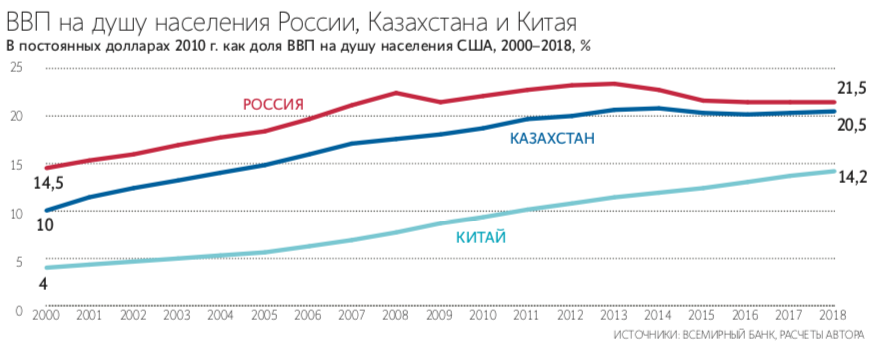
\includegraphics[width=0.68\textwidth]{img/1tbz.png}
    \end{center}
\end{wrapfigure}
\textbf{Авторитарный дедлок.} Более жесткие деспотические режимы политологи называют «авторитарной гегемонией». На выборах здесь авторитарный лидер или правящая партия регулярно получают от 75 до 99\% голосов. Что, однако, свидетельствует не об их популярности, а о том, что они оказывают гораздо более систематическое давление на оппозицию, независимые СМИ и нелояльные элитные группы, т. е. отличаются от предыдущего типа резко возрастающим уровнем репрессивности. Встречаются они сегодня почти исключительно в Азии, Африке и бывшем СССР.

Как показывает опыт ряда азиатских стран, эволюция режима от первого типа ко второму часто происходит на фоне ухудшения экономической динамики. По мере того как экономика играет все меньшую роль в обеспечении легитимности и устойчивости режима, все большую роль начинают играть две другие опоры: репрессии и идеология. В информационной политике режим переходит от фильтрации и ограничения информации к агрессивной пропаганде. Начинаются систематические преследования гражданского активизма, появляются нормы, позволяющие в уголовном порядке преследовать за слова, криминализуется уличная активность граждан.

Именно переход от режима конкурентного авторитаризма к авторитарной гегемонии составил политическое содержание последнего путинского периода – с 2013 по 2019 г. А геополитическая конфронтация выступила в качестве той идеологической рамки, которая легитимирует возрастающую репрессивность.

Хотя Россия выглядит сегодня гораздо более авторитарной страной, чем в 2012 г., этот переход, видимо, следует считать пока незавершенным. Наверное, играют свою роль развитая социальная инфраструктура мегаполисов, уровень европеизированности элит, глубина проникновения интернета и социальных медиа. Ну, и разумеется, экономический застой. Несмотря на это, Путин вряд ли оставит свои усилия по девестернизации России. И это бесплодное (в исторической перспективе) перетягивание каната скорее всего останется главным сюжетом финальной фазы его политической карьеры.


\newpage
\section[Евгений Пригожин]{Пригожин Евгений Викторович}

\textit{Бизнесмен, владелец группы «Конкорд» и ЧВК «Вагнер»}

\textit{Источник \url{https://www.rbc.ru/person/63d280069a79473d6f5e3ce6}}

\textbf{Молодость, образование, родители.} Евгений Пригожин родился в Ленинграде. Его мать Виолетта Кировна Пригожина была медиком и работала в больнице. Отец Виктор Евгеньевич Пригожин рано умер, и ребенка воспитывал отчим Самуил Жаркой. Будучи лыжным инструктором, Жаркой приобщил его к беговым лыжам. В 1977 году Пригожин окончил ленинградскую спортивную школу-интернат № 62 (ныне колледж олимпийского резерва № 1), где учился вместе с пловцом Владимиром Сальниковым и гимнастом Александром Дитятиным, которые впоследствии стали трехкратными чемпионами московской Олимпиады. После школы поступил в Ленинградский химико-фармацевтический институт, получил специальность «провизор-фармацевт». В 2018 году в одном из интервью он сообщал, что институт не закончил.

\textbf{За что сидел Пригожин.} Агентство «Росбалт» (Минюст включил его в реестр СМИ-иноагентов) сообщало, что в ноябре 1979 года Куйбышевский районный народный суд Ленинграда приговорил Пригожина к двум с половиной годам лишения свободы условно по обвинению в краже. По данным Forbes, в 1981 году Ждановский народный районный суд Ленинграда приговорил Пригожина по новым обвинениям в краже, мошенничестве, вовлечении несовершеннолетнего в преступную деятельность и разбое к 13 годам колонии. В 1988 году Пригожин был помилован.

\textbf{Ресторатор, бизнес, карьера.} В 1990 году он стал заниматься бизнесом, начав с продажи хот-догов. Как пишет Forbes, этот бизнес он открыл вместе с отчимом, и часть производства находилась в квартире Пригожина. «Горчицу к хот-догам замешивали прямо у меня на квартире. [...] Приходилось платить бандитам с каждого ларька по \$100», — приводит издание его слова.

В 1991–1997 годах Пригожин управлял сетью частных продовольственных магазинов «Контраст», в 1995 году открыл бар-магазин «Винный клуб» на Васильевском острове в Санкт-Петербурге. В 1996 году, после знакомства с ресторатором Тони Гиром, открыл первый «элитный» ресторан города — «Старая таможня», после появились «Русский китч», «Семь сорок» и «Строгановский дворец».
В том же 1996 году Пригожин основал компанию «Конкорд кейтеринг».

В 1997 году Пригожин открыл ресторан на теплоходе, который получил название New Island и стал на тот момент самым дорогим рестораном Петербурга.
В 1999 году в New Island ужинали премьер-министр Сергей Степашин и директор-распорядитель МВФ Мишель Камдессю.

Пригожин продолжал заниматься розничным фастфудом и с 2002 по 2012 год развивал в Петербурге сеть кафе-блинных под придуманным им названием «Блин! Дональт's». Заведения сети позиционировались как социально значимые, с дешевой едой для местных жителей, блюда в меню получали необычные названия — в частности, там был сэндвич «квадрососисон». Бизнесмен планировал открыть до 20 кафе, однако к 2008 году открылось лишь десять, а с 2009 года компания Пригожина начала закрывать рестораны, последний из которых закончил работать в 2012 году. Сеть фактически послужила основой для создания Пригожиным в дальнейшем формата комбинатов питания. В 2016 году, как писал тогда РБК, Пригожин фактически стал монополистом на рынке школьного питания в Москве.

Строительным бизнесом Пригожин начал заниматься в 2000-х годах в Петербурге. В частности, как писала «Фонтанка», «Конкорд» в районе Лахты построил жилой комплекс «Северный Версаль» из 45 трехэтажных домов в стиле архитектуры Петербурга XVIII—XIX веков.

В 2008 году компания Пригожина ООО «Конкорд менеджмент и консалтинг» (входит в группу «Конкорд») получила участок рядом с парком 300-летия Петербурга для строительства Центра водного туризма. В 2011 году компания обратилась в суд, заявив, что городские власти затягивают выделение участка. В 2012 году суды трех инстанций подтвердили права инвестора. К марту 2016 года компания возвела на участке комплекс «Лахта Плаза» из шести жилых зданий общей площадью 41,9 тыс. кв. м.

В 2010 году компания, принадлежащая жене Пригожина, арендовала в центре Петербурга Дом торгового товарищества «Братья Елисеевы», в котором после реконструкции открылся «Магазин купцов Елисеевых». Летом 2016 года компания добилась права приватизировать здание за 740 млн руб.

Компания Пригожина также сотрудничала с Минобороны: за период c конца 2014 года по середину 2015-го структуры «Конкорда» выиграли тендеры на 10,3 млрд руб. на уборку в казармах и учебных заведениях оборонного ведомства, подсчитывал тогда РБК. Связанная с Пригожиным компания «Мегалайн» получила в 2015 году контракт на 3,3 млрд руб. на строительство военной базы в Валуйках в Белгородской области, она же выиграла на конкурсе контракт на 161,6 млн руб. на строительство военного городка в Омской области. В том же году несколько связанных с Пригожиным компаний выиграли тендеры на жилищно-коммунальное обслуживание военных городков в нескольких областях страны.

\textbf{Фабрика троллей Пригожина.} Имя Пригожина связывают с созданным летом 2013 года Агентством интернет-исследований, которое в прессе называли «фабрикой троллей». В США эту структуру обвиняли во вмешательстве в выборы. Сам Пригожин долгое время это опровергал. В феврале 2023 года бизнесмен заявил, что придумал Агентство интернет-исследований. «Я его создал, я им управлял длительное время. Создано оно было для защиты российского информационного пространства от хамской агрессивной пропаганды антироссийских тезисов со стороны Запада», --- заявил Пригожин.

В 2017 году стало известно о создании структурами Пригожина «фабрики медиа», в которую вошли Федеральное агентство новостей, а также другие связанные с ним издания, в частности «Политика сегодня», «Экономика сегодня» и «Народные новости». Согласно расследованию журнала «РБК», к февралю 2017 года ежемесячная аудитория изданий «фабрики медиа» достигла 36 млн человек, превысив аудиторию агентства «РИА Новости» и «Комсомольской правды». Вскоре эти издания вошли в медиагруппу «Патриот».

В США Пригожина обвинили во вмешательстве в выборы 2016 года и в политический процесс. В феврале 2021 года ФБР назвала Пригожина в числе 13 россиян, которые объявлены в розыск за вмешательство в выборы президента США. Ведомство предложило вознаграждение в размере до \$250 тыс. за сведения, которые помогут заключить бизнесмена под стражу. Пригожин назвал действия бюро «шоу с розыском, как в старые ковбойские времена», и потребовал удалить с сайта ФБР объявление о вознаграждении за информацию о нем.

\textbf{ЧВК Вагнер Евгения Пригожина.} Пригожин — основатель частной военной компании (ЧВК) «Вагнер». Журнал «РБК» писал о полигоне у населенного пункта Молькино в Краснодарском крае, который начал использоваться, предположительно, для подготовки бойцов ЧВК в середине 2015 года. В октябре 2015-го о наборе добровольцев в состав ЧВК и участии ее бойцов в наземных операциях в Сирии, а также в конфликте на территории Луганской и Донецкой народных республик сообщала «Фонтанка». ЧВК получила название «Вагнер» в 2014 году по позывному первого командира подразделения, офицера запаса Дмитрия Уткина.

В США и Евросоюзе заявляли о действиях ЧВК «Вагнер» также в Ливии, ЦАР, Судане, Мозамбике и Мали. Госдепартамент заявлял, что деятельность «Вагнера» в Африке мешает работе миротворцев ООН на континенте.

В июле 2018 года в ЦАР для съемок фильма о деятельности ЧВК направились журналист Орхан Джемаль, оператор Кирилл Радченко и режиссер Александр Расторгуев. По пути к месту съемок их машину атаковали неизвестные вооруженные люди. Журналисты погибли, с места убийства россиян пропали деньги, техника и документы.

США и Евросоюз обвиняли ЧВК «Вагнер» в нарушении прав человека на Ближнем Востоке и в Африке и ввели против компании санкции, которые были ужесточены после начала российской спецоперации на Украине. Санкции были введены в 2016 году и против Пригожина, которого обвинили в связях с ЧВК.

Пригожин долгое время отвергал связь с ЧВК, заявляя, что «крайне удивлен самим фактом существования данной компании и не имеет к ее деятельности никакого отношения». Однако в сентябре 2022 года признался, что именно он является ее создателем. В конце октября 2022-го бизнесмен заявил о создании в Санкт-Петербурге «ЧВК Вагнер Центра», в котором «смогут работать специалисты в области оборонных и информационных технологий с целью повышения обороноспособности России».

\textbf{ЧВК Вагнер на Украине.} Соединения ЧВК активно участвовали в боевых действиях на Украине, в частности под Артемовском (украинское название — Бахмут) и в Соледаре.

Летом 2022 года начали появляться сообщения о посещении Пригожиным тюрем с целью вербовки заключенных в ряды «Вагнера».

\begin{fancyquotes}
    Те, кто не хочет, чтобы воевали ЧВК, заключенные, кто рассуждает на эту тему, кто ничего не хочет делать и в принципе кому эта тема не нравится, детей своих на фронт отправьте. Либо ЧВК и зэки, либо ваши дети — решайте сами

    \begin{flushright}
        Пригожин в сентябре 2022 года\\
        о вербовке заключенных для участия в спецоперации на Украине
    \end{flushright}
\end{fancyquotes}

В ноябре 2022 года телеграм-канал GREY ZONE, который в Совете по правам человека связали с ЧВК «Вагнер», опубликовал видео убийства мужчины, которого назвали бывшим бойцом ЧВК Евгением Нужиным, участвовавшим в спецоперации. На видео мужчина называет свое имя и дает интервью украинским журналистам, заявляя, что добровольно перешел на сторону Киева. Затем Нужина показывают в темном помещении, и его голова примотана к кирпичам скотчем. Мужчина рассказывает, что 11 ноября 2022 года он находился на улице Киева, где получил удар по голове, в результате чего потерял сознание. «Очнулся в этом подвале, где мне сообщили, что меня будут судить», — говорит мужчина на записи, после чего получает удары кувалдой по голове.

После пленения Нужин в интервью украинскому журналисту Юрию Бутусову рассказал, что сам родом из города Перевоз в Нижегородской области и в 1999 году был осужден на 24 года лишения свободы за убийство человека, а затем из-за неудачного побега ему добавили еще четыре года.

Пригожин, комментируя видео, назвал его «прекрасной режиссерской работой». «Что касается окувалдованного, то в данном шоу видно, что он не нашел счастья в Украине, а встретился с недобрыми, но справедливыми людьми», — отметил он.

Позже Пригожин обратился к генпрокурору с просьбой провести доследственную проверку по факту убийства Нужина. 15 ноября уполномоченная по правам человека Татьяна Москалькова заявила РБК, что следственные органы занялись проверкой.

23 ноября Европарламент принял резолюцию, в которой Россия называется страной — спонсором терроризма в связи с военными действиями на Украине. В документе также содержался призыв к странам ЕС признать ЧВК «Вагнер» и входящий в Росгвардию 141-й полк имени Ахмата Кадырова террористическими организациями. После этого пресс-служба Пригожина сообщила, что тот отправил в Европарламент в футляре из-под скрипки «брендированную кувалду [...] с, вероятнее всего, бутафорскими следами крови».

В январе 2023 года США объявили ЧВК «Вагнер» транснациональной преступной организацией. В ответ Пригожин написал письмо в Белый дом с просьбой прояснить, какие преступления совершала эта организация.

Пригожин неоднократно критиковал власти Петербурга и губернатора Александра Беглова. В июле 2022 года он обвинил губернатора в создании помех для бизнеса, после того как структуры, связанные с предпринимателем, не получили контракт на обустройство территории «Горская» и разработку доверили другой компании, несмотря на инвестиционное соглашение. В администрации Петербурга эту точку зрения назвали частным мнением бизнесмена, отстаивающего свои интересы. Беглов заявлял, что действия правительства Петербурга вызывают критику со стороны некоторых «богатых людей, влиятельных людей, которые могут налом проплачивать определенные вещи», не уточняя, кого конкретно имеет в виду. В Кремле, комментируя подобные высказывания Пригожина, заявили, что тот, как предприниматель, «болеет душой за то, что происходит».

\textbf{Призыв к мятежу и уголовное дело.} Вечером 23 июня Пригожин заявил, что российские военные нанесли удар по лагерю ЧВК «Вагнер», в результате чего погибло «погибло огромное количество бойцов». Он обвинил в этом «военное руководство» и пообещал ответ. Позже пресс-служба основателя ЧВК распространила заявление Пригожина, в котором он уточнил, что его намерение «ответить» --- это «не военный переворот, а марш справедливости».

Минобороны утверждения Пригожина опровергло, назвав их «информационной провокацией». В ведомстве подчеркнули, что вооруженные силы «продолжают выполнение боевых задач на линии соприкосновения с вооруженными силами Украины».

Вскоре ФСБ и Генпрокуратура отчитались о возбуждении уголовного дела против Пригожина по статье 279 Уголовного кодекса по факту организации вооруженного мятежа. В ФСБ заявили, что заявления и действия Пригожина фактически являются призывами к началу вооруженного гражданского конфликта на территории и призвали бойцов ЧВК задержать своего лидера. «Призываем бойцов ЧВК не совершать непоправимой ошибки, прекратить любые силовые действия против российского народа, не выполнять преступные и предательские приказы Пригожина, принять меры к его задержанию», — говорилось в заявлении.

Обратился к бойцам ЧВК и генерал Сергей Суровикин. «Я обращаюсь к бойцам и командирам ЧВК «Вагнер». Мы вместе с вами прошли трудный тяжелый путь. Мы вместе с вами воевали, шли на риски, несли потери, вместе побеждали. Мы одной крови. Мы воины... Пока не поздно, нужно и необходимо подчиниться воле и приказу всенародно избранного президента. Остановить колонны, вернуть их в пункты постоянной дислокации», — сказал он в видео, опубликованном военкором Андреем Руденко.

Вечером 24 июня президент Белоруссии Александр Лукашенко сообщил, что провел переговоры с Евгением Пригожиным, они достигли договоренности об остановке движения бойцов ЧВК по территории России. Глава Белоруссии заявил, что бойцам Пригожина дадут гарантии безопасности. Основатель «Вагнера» заявил, что разворачивает свои колонны и уходит в полевые лагеря «согласно плану».

27 июня дело о мятеже было закрыто. Лукашенко заявил, что Пригожин приехал в Белоруссию. «Как я и обещал, если вы хотите какое-то время у нас перекантоваться и прочее, мы вам поможем. Естественно, за их счет», — заявил президент Белоруссии.

Путин заявил, что «организаторы мятежа, предали свою страну и народ». Он также заявил, что содержание ЧВК «Вагнер» полностью обеспечивалось государством. По словам президента, с мая 2022 года по май 2023-го на денежное содержание и стимулирующие выплаты ЧВК государство заплатило 86 млрд и 262 млн руб. «При всем том, что само содержание «Вагнера» было на плечах государства, за год собственник компании «Конкорд» через «Военторг» получил, заработал от государства, поставляя продукты питания и оказывая услуги по питанию в армии, заработал 80 миллиардов рублей», — сказал Путин. Он добавил, что надеется на то, что «в ходе этих работ никто ничего не украл или, скажем так, украл поменьше». По его словам, с этим еще предстоит разобраться.

\textbf{Катастрофа самолета в Тверской области.} Вечером 23 августа 2023 года в Тверской области разбился самолет Embraer Legacy, совершавший рейс Москва — Санкт-Петербург. Как сообщили в МЧС, на борту находились 10 человек, все они погибли. В Росавиации сообщили, что Пригожин был в списке пассажиров самолета. Позже ведомство уточнило, что, по данным авиакомпании, которой принадлежал самолет, бизнесмен действительно был на борту. Также там находится командир ЧВК «Вагнер» Дмитрий Уткин.

Как 24 августа сообщил Владимир Путин, Пригожин в день авиакатастрофы вернулся из Африки. Президент также рассказал, что знал бизнесмена «с начала 90-х годов». «Это был человек сложной судьбы, и ошибки у него были серьезные в жизни, добивался он результатов нужных — и для себя, и для, когда я его просил, для общего дела, как в эти последние месяцы. Он был талантливый человек, талантливый бизнесмен», — добавил Путин.

27 августа СК сообщил, что экспертиза подтвердила гибель Пригожина и остальных пассажиров самолета.

\textbf{Личная жизнь, жена, дети.} Пригожин женат, у него трое детей. Члены семьи Пригожина, в том числе его дети Полина и Павел, в 2022 году попали под санкции ряда западных стран. Под санкции ЕС и Канады также попала мать Виолетта Пригожина (1939 г.р.). Но в марте 2023-го она смогла добиться аннулирования ограничений, введенных против нее Евросоюзом. Суд ЕС установил, что она не владеет компанией «Конкорд Менеджмент и Консалтинг», как считал Брюссель, а родственных связей для включения в санкционный список недостаточно.

В 2003 году Пригожин вместе с детьми Полиной и Павлом написал книгу сказок «Индрагузик», в которой описана сказочная страна Индрагузия.

В сентябре 2022 года Пригожин на странице своей пресс-службы в соцсети «ВКонтакте» сообщил, что его сын в возрасте 18 лет прошел службу в вооруженных силах и через месяц после армии «поехал на войну в Сирию». «С тех пор он постоянно находился и находится в горячих точках в составе ЧВК «Вагнер», где и получил свой первый Черный крест (награда ЧВК. — РБК)», — говорилось в сообщении.

Пригожин награжден орденом «За заслуги перед Отечеством» IV степени «за достигнутые трудовые успехи, значительный вклад в социально-экономическое развитие Российской Федерации, заслуги в освоении космоса, гуманитарной сфере, укреплении законности, активную законотворческую и общественную деятельность, многолетнюю добросовестную работу», и медалями ордена «За заслуги перед Отечеством» I и II степеней. Также в публичных источниках есть фотографии Пригожина со звездами Героя России, Героя Донецкой и Луганской народных республик. В Кремле на вопрос о присвоении Пригожину звания героя закрытым указом президента заявили лишь, что все открытые указы публикуются.

\newpage
\section{Еда на планете становится дефицитом}

\textit{Что будет с ценами на продукты в России и мире}

\textit{Почему продукты на планете постоянно дорожают}

\textit{Источник \url{https://www.kp.ru/daily/27547.5/4814137/}}

Продовольственный кризис \ex{разворачивается}{is unfolding} на нашей планете прямо сейчас. Трудно в это поверить, глядя на переполненные полки супермаркетов. Но нехватку еды, по данным ООН, ощущают на себе уже около 2 млрд человек в 80 странах. А около 20 тысяч человек ежедневно умирает от голода и его последствий.

Последний резкий рост цен на продовольствие случился в 2020 - 2022 годах. И это был уже третий \ex{скачок}{jump} за последние 15 лет. В первой половине 2023 года цены вроде пошли вниз, но в июле --- новый рост. Так в чем причины нехватки еды на планете?

\textbf{Причина № 1. Конфликты и войны.} Это одна из главных причин: 70\% голодающих живут на территориях, где происходят боевые столкновения. И \ed{нынешнее}{нынешний}{present, current} вооруженное \ex{противостояние}{confrontation} на Украине тоже ударило по самым чувствительным точкам --- поставкам энергоносителей, удобрений и сельхозпродукции.

До начала боевых действий Россия и Украина экспортировали на мировые рынки значительные доли пшеницы (18\% и 10\%), ячменя (14\% и 12\%), \ed{подсолнечного масла}{подсолнечное масло}{sunflower oil} (26\% и 37\%). После начала кризиса объемы экспорта сельхозпродукции с Украины сократились на 30 - 40\%. Странам Европы, Азии и Африки пришлось искать новых \ed{поставщиков}{поставщик}{supplier} и выстраивать новые пути доставки, что привело к росту цен.

\textbf{Причина № 2. Природные катаклизмы.} Особенно от этого страдают жители Африки и Юго-Восточной Азии. В 2021 - 2022 годах дефицит осадков здесь достигал 80\%. Грустный итог: с середины 2021 года по апрель 2022-го в Кении и Эфиопии погибло около 3 млн голов скота. Похожая ситуация в Сомали.

А в западной части континента все наоборот: наводнения уничтожают пахотные земли. По оценке ООН, производительность сельского хозяйства в Африке по итогам 2022 года снизилась на 34\%.

Страдают от аномалий погоды Индия, Китай, Южная Америка. Постоянно дают о себе знать течения Эль-Ниньо и Ла-Нинья: температура воды в экваториальной части Тихого океана меняется, влияя на осадки в Азии и Южной Америке.

Не жалеет погода и США. Из-за жары 2022 года урожай пшеницы в Америке сократился вдвое, а на юге Европы погодные аномалии принесли убытки на миллиарды евро...

\textbf{Причина № 3. Энергетический кризис.} Для производства, доставки, упаковки, хранения продуктов нужна энергия --- газ, нефть, электричество. А газ и нефть резко дорожали в 2021 - 2022 годах (цена на голубое топливо взлетала в несколько раз). Последствия этого скачка мир ощущает до сих пор.

\textbf{Причина № 4. Нехватка удобрений.} Современное сельское хозяйство \ex{немыслимо}{unthinkable} без минеральных удобрений, а они постоянно дорожают. С 2022 года этот рынок залихорадило снова: сказались \ed{перебои}{перебой}{interruption} с поставками из России, введение экспортных квот Китаем и подорожавший в 2022 году природный газ --- ключевой компонент при изготовлении азотных удобрений. Проблемы с газом заставили многие страны сократить собственное производство.

Итог --- цены на отдельные виды удобрений подскочили в три раза, что сразу ударило по стоимости продуктов. Нехватка удобрений наверняка скажется и на урожайности.

На мировые цены влияет множество факторов. Стоимость отдельных продуктов может не только расти --- бывает, что цены снижаются. Но, как шутят эксперты, если цены падают на биржах, они не падают на наших кухонных столах. Ведь стоимость сельхозтоваров формируется главным образом после того, как они покидают фермы. Речь о затратах на энергию, обработку, упаковку, доставку, рабочую силу... И каждая из этих позиций из года в год прибавляет в цене. В итоге по пути в магазин продукты дорожают в 2 - 3 раза, а то и больше.

В этом году быстрее других продуктов дорожают зерно, рис, какао и апельсины. Давайте выясним, почему.

\textbf{Нерациональное зерно.} Мировой рынок зерновых \ex{трясет}{is shaking}. В начале марта цены на пшеницу достигали исторического максимума --- \$12,09 за бушель (единица объема для измерения зерна, один бушель равен в среднем 27,21 кг). Затем они падали, снова росли, особенно после того, как Россия вышла из «зерновой сделки». Напряжение между Россией и Украиной играет здесь важную роль, поскольку обе страны --- крупные поставщики этого продукта на мировой рынок.

Сейчас стоимость пшеницы на биржах упала до 6,5 доллара за бушель, но как цены поведут себя дальше, сказать трудно. С одной стороны, замедляется спрос на зерновые корма. С другой - к увеличению потребления зерновых ведет рост населения планеты.

Мировая торговля зерном к 2031 году должна вырасти на 15\%, а пшеница в общем объеме занимает около 40\%. И Россия останется одним из лидеров по экспорту пшеницы на мировой рынок (доля - более 20\%). Оптимизма добавляют и хорошие урожаи в нашей стране.

Сообщения о том, что в России из-за ситуации на зерновом рынке может подорожать хлеб, на днях опроверг Минсельхоз. Здесь уверили: обеспеченность России зерном намного превышает внутренние потребности. Поэтому рост цен на хлеб в этом году будет не выше общей инфляции (по плану --- не более 6,5\%).

\textbf{Рис --- благородное дело.} Цены на рис в этом августе достигли многолетних максимумов. Например, эталонный для экспортеров в Азии тайский белый рис стоил \$650 за тонну - это на 50\% больше, чем в августе прошлого года. Особенно быстро цена на рис стала расти с июля, после объявления Всемирной метеорологической организацией ООН о появлении Эль-Ниньо, вызывающего засухи.

Кроме того, недавно Индия --- крупнейший поставщик риса --- заявила о запрете экспорта 80\% этой продукции, чтобы сдержать рост внутренних цен на этот стратегический для страны товар. Временно запретили экспорт риса ОАЭ и Россия. Но стратегическим продуктом рис остается не только для Индии, а для 40\% населения Земли, особенно в Азии. Он обеспечивает базовое питание 3 млрд человек. И экономисты \ex{опасались}{they feared}, что осенью цены на рис могут вырасти вдвое к прошлому году.

России рост цен пока не грозит. Во-первых, наша страна сама выращивает рис. Его мы ежегодно производим больше миллиона тонн, и этого хватит, чтобы удовлетворить внутренний спрос. Во-вторых, правительство вовремя ввело ограничения на вывоз этого продукта из страны --- теперь у аграриев нет \ed{искушения}{искушение}{temptation} экспортировать рис, пользуясь выгодными для себя ценами.

\textbf{Чао, какао!} Какао-бобы, а точнее, какао-масло, которое из них производят, --- один из главных ингредиентов в производстве шоколада. Дефицит и подорожание какао приведет к росту цен на всю кондитерку.

Стоимость какао-масла выросла с начала года уже на 20\% и приблизилась к максимальному уровню за последние полвека, преодолев в июле \ed{отметку}{отметка}{mark} 3500 долларов за тонну. Причина --- плохая погода в Западной Африке. Ведь как раз на две страны этого региона --- Кот-д' Ивуар и Гану --- приходится 60\% мирового производства какао.

Основатель фабрики ShokoBox Андрей Шарков уверен, что повышения цен на шоколад не избежать и России. Причины -- \ex{подорожание}{rise in price, price hike} сырья на мировых рынках и ослабление рубля. Ведь наш шоколад производится из импортных компонентов.

\begin{fancyquotes}
    Думаю, что осенью нам следует ожидать роста цен на шоколадные изделия в среднем на 10\%, - рассказал Андрей Шарков «КП». - При этом их качество станет хуже.
\end{fancyquotes}

Многие производители попытаются компенсировать рост цен заменой натурального какао-масла дешевыми заменителями. Российский рынок не слишком требователен к качеству, но те, кто ценит настоящий шоколад, почувствуют разницу. И качественные продукты без заменителей подорожают еще больше. Мой прогноз --- на 20\%.

\textbf{Нету сладких апельсинов.} Бразилия была и остается крупнейшим мировым поставщик\'{о}м концентрата для производства апельсинового сока. Но в этом году в стране \ex{неурожай}{bad harvest, crop failure}, цены поползли вверх. Масла в огонь подлили неблагоприятная погода и плохой урожай цитрусовых в США, Мексике и Испании. В итоге за год стоимость фунта замороженного концентрата апельсинового сока выросла с 2 до 3 долларов.

В России цены на апельсины росли с 2020 года. А этим летом наши торговые сети столкнулись с их дефицитом, так что дорожать они, видимо, будут и дальше. Замороженный концентрат апельсинового сока уже подорожал в России на 30\%. Что неизбежно приведет к пропорциональному росту цен.

\textbf{В ТЕМУ}

\textbf{Пицца против окрошки}

\textbf{Национальные блюда тоже бьют по кошельку}

Официальные цифры инфляции не всегда отражают то, как ощущают на себе подорожание продуктов обычные граждане. В ЕС, например, продовольственная инфляция составляет порядка 12,5\%. Но если взять популярную в Италии пиццу «Маргарита», то ее цена в январе 2023-го, по данным Bloomberg, выросла к январю 2022 года на 25\%. Притом, что официальная инфляция в Италии за этот период составила 10,7\%. А все потому, что сильно взлетели цены на сыр и муку.

Похожая ситуация с национальным блюдом испанцев паэльей. Она за год подорожала на 19\% при общей инфляции в Испании 6\%. Сказался рост цен на оливковое масло, овощи и бобы.

На 20\% подорожал классический британский завтрак (сюда входят бекон, колбаски, яйца, тосты и напиток). Причина - рост цен на молоко, хлеб и яйца. Кстати, в США именно яйца рекордно взлетели в цене - в начале 2023 года они стоили на 60\% дороже, чем годом ранее.

А вот окрошка подорожала за год всего на 6\%. Виноваты в основном овощи. Редис подорожал к прошлому году почти на треть, огурцы - на 25\%, зеленый лук - на 5\%. Даже квас прибавил в цене 6\%. Зато картофель и яйца подешевели.

\textbf{ТОЛЬКО ЦИФРЫ}

29,3\% всего населения планеты испытывают умеренную или серьезную нехватку продовольствия.

Более 345 млн человек столкнутся в 2023 году с «высоким уровнем отсутствия продовольственной безопасности». По сути --- будут \ed{недоедать}{недоедать/недоесть}{to be undernourished, to not eat enough}.

14 из 15 стран с наибольшим отсутствием продовольственной безопасности находятся в Африке.

По данным ФАО ООН и Всемирной продовольственной программы ООН.












\chapter{Культура, обычаи и традиции}

\section{Праздники}
\subsection{Рождеств\'{о} Христ\'{о}во}
Рождеств\'{о} Христ\'{о}во --- праздник \explain{правосл\'{а}вного}{правосл\'{а}вный: orthodox} календаря, \explain{устан\'{о}вленный}{established} 7 января (25 декабря ст стиля).

По народному календ\'{а}рю этот день являлся днём з\'{и}мнего \explain{солнцевор\'{о}та}{солнцевор\'{о}т: solistice}, когда начиналось \explain{проб\'{у}ждение}{awakening (пробуждать/пробудить: to waken)} солнца после его дл\'{и}тельного з\'{и}мнего сна. Рождество Христово почиталось по всей России и по своей \explain{значимости}{значимость: significance} в православном календар\'{е} стояло на втором месте после П\'{а}схи. В русской деревне оно \explainDetail{отмеч\'{а}лось}{отмечаться/отметиться}{to celebrate} обычно в течение трёх дней и начиналось с посещения хр\'{а}ма, которое считалось у крестьян делом желательным, но не строго обязательным.

Рождество также отмечалось двумя тр\'{а}пезами: в рожд\'{е}ственский \explainDetail{соч\'{е}льник}{(рождественский) соч\'{е}льник}{Christmas eve; кан\'{у}н: eve} (канун праздника) и \explain{непосредственно}{directly} в Рождество.

Трапеза \explain{накануне}{on the eve of} праздника начиналась с появлением на небе первой вечерней звезды. На стол \explainDetail{подавали}{подавать/подать}{to serve} блины или оладьи с медом, \explain{постные}{пост: fasting} пироги с грибами, картофелем, кашей, пресные пирожки с ягодами, а также кутью из крупных зерен пшеницы с ягодами.

Тр\'{а}пеза, проходившая в день Рождества, предполагала богатый и \explain{разнообразный}{diverse} обед, во время которого подавалось множество мясных и молочных блюд, пирогов.

Рождество б\'{ы}ло первым днём \explain{выполнения}{performance; execution; effectuation} различных \explain{обр\'{я}дов}{обр\'{я}д: ritual}, которые должны б\'{ы}ли \explainDetail{обеспечить}{обеспечивать/обеспечить}{to provide} \explain{благополучие}{well-being} в наступающем солнечном году, \explain{предохранить}{(предохранять): to protect} от \explain{бед}{беда: misfortune; trouble} и несчастий дом, семью, \explain{скот}{cattle}, узнать будущее.

В рожд\'{е}ственский сочельник начинали колядов\'{а}ть. Группы детей, подр\'{о}стков, молодых мужчин и женщин обходили крестьянские дом\'{а} и \explain{исполн\'{я}ли}{исполнять/исполнить: to perform; to carry out} песни (кол\'{я}дки) с величаниями и пожеланиями хоз\'{я}йственного благопол\'{у}чия и семейного \explain{дов\'{о}льства}{довольство: contentment}. Начинались \explain{гад\'{а}ния}{гад\'{а}ние: fortune telling, divination} о судьбе.

С днём Рождества б\'{ы}ли св\'{я}заны разл\'{и}чные \explainDetail{прим\'{е}ты}{примета}{omen}.
Русские крестьяне верили в то, что травы и зернов\'{ы}е культуры будут хорош\'{и}, если на Рождество лежат \explain{глуб\'{о}кие}{глуб\'{о}кий, глуб\'{о}кая, глуб\'{о}кое, глуб\'{о}кие: deep} снег\'{а}; если в Рождество на небе много звёзд --- можно ждать бог\'{а}того \explain{урож\'{а}я}{(noun) harvest} гор\'{о}ха, а если в этот день сильная метель, то пчелы будут хорошо роиться. (По И. Шангиной)


\subsection{Масленица}
М\'{а}сленица --- большой народный праздник \explainDetail{проводов}{проводить}{to see off; пр\'{о}воды: used only in plural} зимы. В традиционном русском \explainDetail{быт\'{у}}{быт}{life; everyday life (в быт\'{у}: locative; in life)} эта неделя ст\'{а}ла самым \explain{\'{я}рким}{яркий: bright; brilliant; outstanding}, наполненным радостью жизни праздником.

Масленица отмечалась по всей России и в деревнях, и в городах. Её празднование считалось для всех русских людей обязательным: «Хоть себя заложи, а масленицу проводи». Неучастие в масленичном веселье могло повлечь за собой, \explain{по поверью}{according to the belief}, «жизнь в г\'{о}рькой беде».
Первые три дня масленой недели шла \explain{подготовка}{preparation} к празднику: привозили дров\'{а} для масленичных костров, убирали \explain{избы}{изба: hut; little house}. Основные \explain{пр\'{а}зднества}{пр\'{а}зднество: festivals} \explain{приходились}{happen} на четверг, пятницу, субботу, воскресенье --- дни широкой масленицы.

Все масленичные развлечения проходили обычно на улице. \explain{Нар\'{я}дно одетые люди}{elegantly dressed people} участвовали в праздничном \explain{гулянье}{celebration}, поздравляли друг друга, шли на ярмарку, удивлялись чудесам, которые показывали в балаганах --- передвижных театрах, радовались кукольным представлениям и «медвежьим потехам» --- выступлениям вожака с медведем. Масленичный комплекс включал в себя такие развлечения, как катание с гор, катание на санях, кулачные бои, шествия ряженых и др. В масленицу звучало много песен, прибауток, приговоров.

Прощ\'{а}лись с масленицей всегда в воскресенье.
В этот день жгли костры, которые символизировали солнце и должны были \explain{способствовать}{ (поспособствовать) to contribute} скорейшему пробуждению природы, и жгли \explain{ч\'{у}чело}{scarecrow} Масленицы. (По И. Шангиной)



\subsection{П\'{а}сха (Воскресение Христово)}
Название П\'{а}сха происходит от древнееврейского слова «песах» (прохождение). В русский язык слово «пасха» пришло из греческого, вместе с принятием православия, но у многих славянских народов праздник Воскресения Христова называется \explain{иначе}{differently; otherwise}: у украинцев --- великдень, у белорусов --- вяликдзень, у болгар --- великден, у поляков ---Wielkanoc, у чехов --- Velikanoc и т.д.

Нет праздника более торжественного, более радостного, чем Светлое
Христово Воскресение. Конец марта --- апрель --- это уже время прихода
настоящей весны, её \explainDetail{победы}{поб\'{е}да}{victory}
над зимними холодами, праздник \explainDetail{возрождения}{возрожд\'{е}ние}{rebirth},
воскрешения природы. Вместе с тем это и начало нового
\explainDetail{сельскохозяйственного}{сельскохоз\'{я}йственный}{agricultural (of the agric. economy)}
года, начало \explainDetail{полев\'{ы}х}{полев\'{о}й}{related to a field} работ
--- \explain{вспашки}{plowing} и \explain{сева}{(сев) sowing}.

В Древней Руси именно с весеннего \explainDetail{равноденствия}{равноденствие}{equinox}
начинался новый год, а чтобы посевы \explain{благополучно}{safely} взошли и вызрели,
скот давал приплод, н\'{у}жно было исполнить различные магические обряды.
Один из таких \explain{сохранившихся}{survived} до настоящего времени обрядов
--- пасхальная тр\'{а}пеза, когда единственный раз в году готовятся блюда,
которые в другие дни к столу не \explainDetail{подаются}{подавать/подать}{to serve}:
куличи и крашеные яйца.

Крашеными яйцами \explainDetail{обменивались}{обмениваться/обменяться}{to exchange},
их дарили родным, соседям, пришедшим поздравить, их брали с собой, отправляясь
в гости, раздавали нищим. (По Л.С. Лаврентьевой и Ю.И. Смирнову)

\newpage
\section{За здоровье или на здоровье?}

\textit{Источник: \url{http://really-easy-russian.blogspot.com/2012/12/blog-post_30.html}}

Есть хорошая русская традиция: приглашать к себе домой в гости, готовить много разной ед\'{ы} и сидеть долго за столом. За столом гости наливают себе в бокалы – кто наливает вино, кто водку, кто сок. Все вместе \ed{ч\'{о}каются}{чокаться/чокнуться}{to clink glasses (ч\'{о}каюсь, ч\'{о}каешься, ч\'{о}каются / ч\'{о}кнусь, ч\'{о}кнешься, ч\'{о}кнутся)} и потом пьют.
Перед тем как выпить, кто-то обычно говорит тост – пожелание. Например, такой тост «Давайте выпьем за др\'{у}жбу!». Раньше в\'{е}рили, что напиток, которые все пьют вместе, не только объединяет всех, но обладает магической, волшебной силой, поэтому слова-пожелания обязательно \explain{сбудутся}{come true}.
Вот почему России пьют обычно за что-то или кого-то: за здоровье, за любовь, за успехи, за встречу, за хорошее настроение, за радость, за хозяйку дома, за её мужа, за детей и т.д.

В древности в\'{е}рили не только в волшебную силу напитка, которые пили вместе, но и в магическую силу еды. Когда гость \explain{хвал\'{и}л}{praised} еду, которую приготовила хозяйка, она благодарила его и отвечала – и сегодня отвечает: «На здоровье!»\footnote{like ``cheers''}. «На здоровье» выражает, во-п\'{е}рвых, благодарность, это вариант слова «спасибо».
Во-втор\'{ы}х, желание, чтобы еда принесла гостю только хорошее, особенно здоровье. Поэтому когда мы говорим в ресторане, в гостях «спасибо», часто в ответ слышим – «на здоровье!».

Итак, когда поднимаем бокалы и ч\'{о}каемся -- говорим только «за здоровье!», когда гости у вас дома хв\'{а}лят ваше вкусное блюдо – отвечаете «на здоровье!».

\newpage
\section{Как живет Лаос}

\textit{Нищая страна из «опиумного треугольника» с атмосферой, которой не найдешь нигде в мире}

\textit{Источник: \url{https://lenta.ru/articles/2022/10/14/laos/}}

Одна из самых раскрученных достопримечательностей Юго-Восточной Азии — так называемый Золотой треугольник, где сходятся границы трех стран: Таиланда, Лаоса и Бирмы. Раньше в этом регионе были плантации опиумного мака, поэтому неофициально он называется Опиумный треугольник. Еще в прошлом веке здесь происходили войны между мафиозными группировками, а «страшное зелье» распространялось контрабандой по всему миру. Такое положение дел сохранялось до начала 1990-х годов, пока армии Таиланда, Бирмы и Лаоса не разгромили синдикат. В 1996 году главный наркобарон Кхун Са предал своих подельников и бежал. Российский военный репортер Игорь Ротарь отправился в сердце Золотого треугольника и рассказал, чем его впечатлили местные жители. О его приключениях — в материале «Ленты.ру».

\textbf{Путешествие во времени}

В Таиланде былую славу Золотого треугольника превратили в мощный туристический бренд. Толпы туристов на комфортабельных автобусах возят на стык тайской, бирманской и лаосской границ. Здесь, с тайского берега, сидя в хороших ресторанах, туристы любуются видами Лаоса и Мьянмы или катаются на лодках по главной водной артерии Юго-Восточной Азии — реке Меконг.

В этом же месте расположены аж два музея опиума. В одном из них даже есть небольшая маковая плантация. Однако Таиланд российскими туристами изучен уже вдоль и поперек, а вот в лаосской и бирманской части Золотого треугольника гораздо больше самобытности и нехоженых троп.

Лаосскую визу на месяц можно купить за 40 долларов прямо на границе, но россиянам, в отличие от американцев, разрешается пребывать в стране без визы до 30 дней. Оказаться в Лаосе после Таиланда — все равно что переместиться на машине времени лет на сто назад. Почти тот же язык, та же культура и пища, но все в разы беднее и хуже.

Дороги совершенно разбитые. Асфальт ужасного качества проложен только между крупными городами, а между деревнями обычные проселки, превращающиеся в сезон дождей в сплошное грязное месиво. Убогие мостики на реках раскачиваются, и ехать по ним на мотоцикле очень опасно. Живут местные в традиционных домах на сваях, поскольку периодически здесь случаются наводнения. Спят вповалку, готовят на кострах

\begin{center}
    {\Huge
        30 дней
    }

    {\Large
        россияне могут пребывать в Лаосе без визы
    }
\end{center}


По-английски не говорит практически никто. К тому же озвученную транскрипцию местных названий на латинице лаосцы не понимают — латинский алфавит они не знают. Скажем, я остановился в городке Luang Namatha, но когда произносил это словосочетание в разных вариантах, меня не понимали, прочитать же название городка на латинице были не в состоянии.

К слову, цифры у лаосцев тоже другие, поэтому понять, сколько стоит номер в отеле, — серьезная проблема. Кстати, неграмотность среди лаосцев и сегодня составляет 20 процeнтов, а на территориях, относящихся к Золотому треугольнику, наверняка даже больше.

Интересно, что в Лаосе, бывшей французской колонии, многие надписи на государственных учреждениях дублируются по-французски. Для кого это делается — остается загадкой, ведь французского языка местные тоже не знают. Впрочем, какое-то положительное влияние французов все же есть. Так, в отличие от Таиланда, здесь даже в небольших городках можно купить белый хлеб.

\begin{fancyquotes}
    Цены тоже очень странные. Половина жареного цыпленка на рынке стоит меньше доллара, приблизительно столько же — обед в местном кафе, но меню на английском в нем нет, а пища часто выглядит не слишком аппетитно. Если же в ресторане есть меню на английском, что большая редкость, то обед уже потянет на десять долларов
\end{fancyquotes}

Шикарный номер в отеле тоже будет стоить около десяти долларов, то есть дешевле, чем в Таиланде. А вот аренда скутера обойдется в девять долларов, то есть в три раза дороже, чем в соседней стране. Импортные продукты тоже гораздо дороже, чем по ту сторону границы.

\textbf{Национальный характер}

Французские колонизаторы придумали такой афоризм: «Вьетнамцы сажают рис, кхмеры за ним следят, а лаосцы просто смотрят, как он растет». Забавно, что французы так и не смогли справиться с ленью лаосцев и были вынуждены смириться с ней.

Действительно, разница с Таиландом очень ощутима. Лаосцы гораздо медлительнее и заторможеннее соседей. Они искренне хотят выполнить работу хорошо, но делают ее как-то вяло. Создается ощущение, что лаосцы, несмотря на бедность, вообще равнодушны к деньгам.

При этом они очень добродушны и приветливы с туристами. Когда у путешественника случаются какие-то проблемы, они всегда приходят на помощь и, как правило, отказываются брать деньги. Здесь, в отличие от многих бедных стран, не принято обманывать и «разводить» отдыхающих. Преступность в сельском Лаосе тоже практически отсутствует.

Некоторые этнологи объясняют инертность лаосцев тем, что большинство из них — приверженцы буддийского направления Тхеравада, согласно которому материальные блага и карьера несущественны. Однако к той же ветви буддизма принадлежат большинство тайцев, но они больше приспособлены к работе. Самое разумное объяснение — то, что тайцы почти насильно были приучены к капитализму на рубеже XIX-XX веков королем-реформатором Рамой Пятым, а вот лаосцы так и остались жить в раннефеодальном обществе.

\textbf{В краю племен}

Горная долина Луангнамтха — одна из главных достопримечательностей лаоской части Золотого треугольника. Это настоящий этнографический музей под открытом небом. Здесь среди горных джунглей и рисовых полей живет множество племен — как местных, так и переселившихся из Южного Китая и Вьетнама. Часть племен исповедуют буддизм, часть — язычество, или, если быть точным, анимизм.

\begin{fancyquotes}
    Местные язычники сжигают покойников в священном лесу, а над урнами с их прахом водружают шесты и флаги. В деревнях здесь можно попить рисовой водки, а также изучить ручное ткачество
\end{fancyquotes}

И в тайской, и в бирманской, и в лаосской части Золотого треугольника очень много монастырей и монахов. Но в Лаосе есть интересная особенность: среди послушников здесь в основном дети, причем, судя по их поведению, не очень религиозные. Так, например, я видел, как двенадцатилетние послушники курили.

Дело в том, что при монастырях есть школы, где послушники изучают как светские, так и теологические предметы. Скорее всего, в нищем Лаосе отправить мальчика в монастырь — это просто способ прокормить его и дать ему элементарное образование.

\textbf{Homestay по-местному}

Поселился я в homestay в небольшой деревеньке одного из племени анимистов, чьи предки переселились в Лаос из Вьетнама в конце XIX века. Жилье представляло собой традиционную бамбуковую хижину, сразу за которой начинались рисовые поля. Ночлег и еда обошлись всего в 12 долларов. Хозяева были очень радушны, но не без характерных для Лаоса особенностей.

Так, например, зная, что я выпиваю две чашки кофе, мне их подавали сразу — видимо, чтобы не варить кофе дважды. А когда я захотел купить бутылочку вина, хозяева не поняли, как снять упаковку с горлышка бутылки. Впрочем, спустя какое-то время с этой задачей они справились, но под упаковкой оказалась пробка, а штопор им найти так и не удалось.

Но это все мелочи, ведь в Лаосе царит настоящий покой, которым можно наслаждаться, катаясь на велосипеде и глядя на великолепные пейзажи. По вечерам я иногда выбирался в деревню, играл с местными детьми в перетягивание каната и даже пел под мобильник в импровизированном караоке. Забавно, что после дождя местные дети скатывались с горки по грязи так же, как наши ребятишки — по снегу.

Иногда я выбирался на вечернюю службу в ближайший сельский монастырь. Но, увы, задерживаться там долго не получалось. Дело в том, что в буддийских храмах часто есть собаки, их не прогоняют даже во время богослужений. Так вот, псы начинали лаять на меня, хотя на прихожан-лаосцев не реагировали. Наверное, у меня плохая карма.

\textbf{Лас-Вегас по-лаосски}

Впрочем, несколько лет назад в лаосской части Золотого треугольника появилось развлечение совсем другого рода. В свободной экономической зоне, как раз на стыке с тайской и бирманской границей, китайские мафия соорудила поселок с казино, шикарными отелями, ресторанами и борделями.

\begin{fancyquotes}
    Как отметила побывавшая в местных игорных домах корреспондентка BBC, это квинтэссенция китча. Среди клиентов казино лаосцев почти нет, все туристы здесь из Китая и Таиланда
\end{fancyquotes}

Интересно, что нечто подобное уже существовало в бирманском городке Монг Ла, расположенном прямо на китайской границе. В реальности город и его окрестности контролируют сепаратисты, создавшие здесь непризнанное государство Шан.

Я побывал в этом городке около 20 лет назад. Попал я туда почти случайно. Бродя по бирманским горам, неожиданно наткнулся на деревеньку, где остановились на постой мьянманские военные. Бравые солдаты чувствовали себя здесь как дома. Они качались в гамаках на верандах хижин, лениво наблюдая за тем, как крестьянки режут кур, предназначенных на обед этим непрошенным гостям.

Офицеры пригласили меня разделить с ними трапезу. «Об армии в Мьянме говорят всякое, а на самом деле мы просто смотрим за порядком, помогаем людям», — на хорошем английском начал беседу старший из военных.
В диалоге офицер упомянул непризнанное государство Шан и сказал, что туда можно поехать иностранцу.

Добраться до мятежников, как выяснилось, можно даже на обычном такси. Пока мы ехали, подпрыгивая на многочисленных кочках и рытвинах, я вспоминал мьянманские города, где даже электричество подается с перебоями, и с тоской размышлял, какой дырой должно быть это непризнанное государство Шан. И вдруг через три часа пути я неожиданно попал в другой мир.

Проселочная дорога сменилась великолепным шоссе, а вместо привычных для Мьянмы хижин стали появляться аккуратные каменные дома с надписями на китайском. На одном из них даже красовалась реклама Coca-Cola, которая запрещена в Мьянме как чуждый местному образу жизни напиток.

После нищей и неухоженной Мьянмы Монг Ла производил впечатление города с другой планеты: украшенные неоновой рекламой небоскребы, великолепные магазины и изысканные рестораны с самой экзотической пищей (около кафе в качестве приманки для гурманов стояли огромные аквариумы с питонами и другими змеями).

\begin{fancyquotes}
    Электричество и интернет сюда поступают из Поднебесной, а китайские сим-карты работают без роуминга. Бирманские деньги здесь не принимают, расплачиваться можно только юанями. В Китае Монг Ла называли «азиатским Лас-Вегасом» или «Городом греха». И действительно, казино были открыты практически в каждом отеле, а все клиенты были приезжими из Китая
\end{fancyquotes}

Игорный бизнес стал развиваться здесь в начале 1990-х годов, когда местные наркобароны решили покончить с прежним ремеслом и найти ему альтернативу. Как бы подводя итоги своей деятельности, мафия даже открыла музей опиума, посвященный нелегкой деятельности торговцев смертью.

Впрочем, как я убедился, азартными играми список разрешенных здесь пагубных человеческих пристрастий не ограничивался. Однажды мне навстречу попались полупьяные молоденькие европейки, которые шли покачиваясь и отчетливо матерились по-русски. Они оказались родом из Благовещенска, древнейшую профессию начали осваивать еще в Китае, однако затем, во избежание конфликтов с полицией, перебрались в более терпимый Монг Ла, где проституция фактически разрешена.

Китайские власти были недовольны существованием такого криминального анклава, но их терпению пришел конец, когда дочка крупного партийного деятеля проиграла в Монг Ла несколько сотен тысяч долларов. На короткое время Пекин ввел в государство Шан войска, и в 2005-м все казино в Монг Ла были закрыты. Однако, как говорится, свято место пусто не бывает. Китайская мафия попросту перенесла свой бизнес подальше от китайской границы — так и возник лаосский Лас-Вегас.

Лаос — определенно для искушенных туристов. Здесь можно умиротворенно отдохнуть в горах с погружением в местный быт либо покутить в казино и шикарных ресторанах (или даже в борделях). Ну, а на чем именно сделать акцент, каждый выбирает для себя сам.

\newpage
\section{Хэллоуин: что за праздник и что про него рассказать детям}

\textit{Споры относительно пр\'{а}зднования Хэллоу\'{и}на не утихают каждый год. Как же относ\'{и}ться к дате?\footnote{What about the date?} Мы оставляем решение за вами и \ed{д\'{е}лимся}{дел\'{и}ться + \textit{чем}}{to share} историей праздника.}

\textit{Источник: \url{https://gorodskayaferma.ru/blog-halloween}}



\textbf{Откуда он появился?}

Кельтские племена праздновали Новый год в последний день октября и в\'{е}рили, что в ночь с 31 октября на 1 ноября граница между миром жив\'{ы}х и миром мёртвых стир\'{а}лась. А чтобы обмануть злых духов и не \explain{попасться}{to get caught} ими, люди \explain{прикидывались}{pretended} им. Отс\'{ю}да традиция \explain{наряжаться}{to dress up} в \ed{устрашающие}{устрашать}{to frighten} костюмы.

\textbf{Причём здесь тыква?}

Тыква ст\'{а}ла символом праздника по логичной причине. Конец октября --- время сб\'{о}ра урож\'{а}я, а крупный овощ считался символом плодородия. Время это называлось Самайн. Считалось, что огонь внутри тыквы защищал от злых духов и \explain{отп\'{у}гивал}{scared away} \ed{прочую}{прочий}{other} \explain{н\'{е}чисть}{evil spirit}.

\textbf{Хэллоуин праздновали всегда?}

С принятием христианства люди отказались от идеи праздновать Самайн. Но в последствии, древний праздник вновь возродился — 1 ноября католики стали отмечать День всех Святых («All Hallows Even») и люди вернулись к кельтским традициям — стали наряжаться в устрашающие костюмы, зажигать огонь в тыкве и прятаться от духов.

\textbf{Как праздник пришёл к нам?}

Про Хэллоуин мы узнали благодаря массовой культуре и глобализации, а вот общих культурных корней у нас с этой датой действительно нет.

\textbf{А есть ли аналоги в нашей культуре?}

Несколько славянских праздников очень напоминают традиции Хэллоуина. Например, на Святки принято калядовать — стучаться в дверь к незнакомцам и просить угощение. К тому же, в этот пер\'{и}од (между Рождеством и Крещением) считается, что наш мир остаётся без защиты от нечистых сил и именно в эти дни люди могут гадать и переодев\'{а}ться в духов.

Ещё один похожий праздник — Велесова ночь. Кстати, отмечалась она в те же даты, что и Хэллоуин — в ночь с 31 октября на 1 ноября. Так же считалось, что в это время граница между мирами исчезает. Только наши \explain{пр\'{е}дки}{ancestors} ожидали вполне конкретных духов -- ум\'{е}рших р\'{о}дственников, которые могли вернуться на землю, дать совет и поговорить с живыми. Наряжаться в нечисть было не принято, а вот зажигать свечи — да. Огонь был зн\'{а}ком для душ, которые \'{и}щут путь.

\textbf{Какие ещё похожие праздники есть в мире?}

1 и 2 ноября в Мексике тоже \ed{почитают}{почитать}{revere} умерших, праздник называется Día de Muertos. В эти дни умерших родственников пышно встречают: чтобы они могли найти путь, города наполняются миниатюрными \ed{страшилками}{страш\'{и}лка}{short children's horror story}: марципановыми и шоколадными \ed{гробами}{гроб}{coffin} и черепами. На улицы выходят люди в костюмах скел\'{е}тов, а ночью народ уходит на кладбища --- прибираться на могилах и праздновать.

В начале ноября в Перу в городе Пуно празднуют La Diablada. Жители в \ed{красочных}{красочный}{colourful} костюмах посвящают танец духам озера Титикака. Танец рассказывает о добре и зле.

С 30 апреля на 1 мая в Германии отмечают Вальпургиеву ночь. Дома украшают фигурками ведьм. А вот в Скандинавии наоборот защищаются от ведьм — жгут костры и шумят, чтобы отпугнуть их.

В мае в Великобритании город Эдинбург очень гордится своими \ed{привидениями}{привид\'{е}ние}{ghost}, которыми по рассказам жителей, населён каждый дом. Местные даже устраивают в честь них фестиваль, где можно прогуляться по тр\'{о}пам приведений, послушать рассказы м\'{е}диумов или устроить спиритический сеанс.

\textbf{Что будет на Городск\'{о}й ф\'{е}рме на ВДНХ на Хэллоуин?}

30 и 31 октября на Городской ферме на \explain{ВДНХ}{выставка достижений народного хозяйства} будет страшно весело! Мы придумали развлекательную и стилизованную программу с ужасным \ed{квестом}{квест}{quest}, кошмарными мастер-классами, \ed{жуткими}{жуткий}{spooky} угощениями, кинопоказом, сказками и конкурсом на лучший карнавальный костюм. Участвуйте в конкурсе и выигрывайте очень полезный приз! Ждём вас в гости!
\chapter{Сказки}
\section{Сестрица Алёнушка и братец Иванушка}
% https://deti-online.com/skazki/russkie-narodnye-skazki/sestrica-alyonushka-i-bratec-ivanushka/
% https://www.youtube.com/watch?v=UDaOREoItE8
Жили-были стар\'{и}к да стар\'{у}ха, у них был\'{а} дочка Алёнушка да сын\'{о}к Иванушка. Старик со старухой умерли. Остались Алёнушка да Иванушка одни-одинёшеньки. Пошла Алёнушка на работу и братца с собой взяла. Идут они по д\'{а}льнему пут\'{и}, по шир\'{о}кому п\'{о}лю, и захотелось Иванушке пить.
%
\begin{dialogue}
    \item Сестр\'{и}ца Алёнушка, я пить хочу!
    \item Подожди, братец, дойдем до кол\'{о}дца.
\end{dialogue}
%
Шли-шли, -- солнце высоко, колодец далёко, жар \explainDetail{донимает}{донимать}{(colloq.) to bother, harass}, пот выступ\'{а}ет. Сто\'{и}т коровье коп\'{ы}тце\footnote{hoof (diminutive of коп\'{ы}то)} полн\'{о} водицы.
%
\begin{dialogue}
    \item Сестрица Алёнушка, хлебну\footnote{(colloq.) to drink} я из копытца!
    \item Не пей, братец, телёночком станешь!
\end{dialogue}
%
Братец послушался, пошли дальше. Солнце высоко, колодец далёко, жар донимает, пот выступает. Сто\'{и}т лошадиное копытце полно водицы.
%
\begin{dialogue}
    \item Сестрица Алёнушка, напьюсь я из копытца!
    \item Не пей, братец, жеребёночком станешь!
\end{dialogue}
%
\explainDetail{Вздохнул}{вздых\'{а}ть/вздохн\'{у}ть}{sigh} Иванушка, опять пошли дальше. Идут, идут, -- солнце высоко, колодец далёко, жар донимает, пот выступает. Сто\'{и}т к\'{о}зье копытце полно водицы. Иванушка говорит:
%
\begin{dialogue}
    \item  Сестрица Алёнушка, мочи нет: напьюсь я из копытца!
    \item  Не пей, братец, козлёночком станешь!
\end{dialogue}
%
Не послушался Иванушка и нап\'{и}лся из к\'{о}зьего копытца. Нап\'{и}лся и стал козлёночком\dots Зовёт Алёнушка братца, а вместо Иванушки бежит за ней беленький козлёночек. Залилась\footnote{flooded} Алёнушка слез\'{а}ми, села на стож\'{о}к -- плачет, а козлёночек в\'{о}зле неё скачет. В ту пору ехал мимо купец:
%
\begin{dialogue}
    \item О чём, красная девица, плачешь?
\end{dialogue}
Рассказала ему Алёнушка про свою беду. Купец ей и говорит:
\begin{dialogue}
    \item Под\'{и} за меня замуж. Я тебя наряж\'{у} в златосеребро, и козлёночек будет жить с нами.
\end{dialogue}
Алёнушка под\'{у}мала, под\'{у}мала и пошла за купца замуж. Стали они жить-поживать, и козлёночек с ними живёт, ест-пьёт с Алёнушкой из одной чашки. Один раз купца не было д\'{о}ма. \explainDetail{Откуда не возьм\'{и}сь}{откуда не возьм\'{и}сь}{out of the blue} прих\'{о}дит \explain{в\'{е}дьма}{witch}: стала под Алёнушкино окошко и такто ласково начал\'{а} звать её куп\'{а}ться на реку\footnote{произношение: н\'{а}реку}. Привела ведьма Алёнушку на реку. \explainDetail{Кинулась}{кид\'{а}ться/к\'{и}нуться}{to throw oneself, to fling oneself, to dash, to rush, } на неё, привязала Алёнушке на шею камень и бр\'{о}сила её в в\'{о}ду. А сам\'{а} оборот\'{и}лась Алёнушкой, \explainDetail{нарядилась}{наряж\'{а}ться/наряд\'{и}ться}{to dress as someone, to imitate} в её пл\'{а}тье и пришла в её хор\'{о}мы. Никто ведьму не \explain{распозн\'{а}л}{recognised}. Купец вернулся -- и тот не распознал.

Одному козлёночку всё было ведомо. Повесил он голову, не пьет, не ест. Утром и вечером ходит по бережку около воды и зовёт:
\begin{dialogue}
    \item Алёнушка, сестрица моя! Выплынь, выплынь на бережок\dots
\end{dialogue}

Узнала об этом ведьма и стала просить мужа \explain{зарежь}{slaughter} да зарежь козлёнка.
Купцу жалко было козлёночка, \explain{привык}{got used to + \textit{дат.}} он к нему. А ведьма так пристаёт, так упрашивает, --- делать н\'{е}чего, купец согласился:
%
\begin{dialogue}
    \item Ну, зарежь его\dots
\end{dialogue}
%
Велела ведьма разложить костры высокие, греть котлы чугунные, точить ножи булатные.
Козлёночек проведал, что ему недолго жить, и говорит названому отцу:
%
\begin{dialogue}
    \item Перед смертью пусти меня на речку сходить, водицы испить, кишочки прополоскать.
    \item Ну, сходи.
\end{dialogue}
%
Побежал козлёночек на речку, стал на берегу и жалобнёхонько закричал:
%
\begin{dialogue}
    \item   Алёнушка, сестрица моя! Выплынь, выплынь на бережок.
    Костры горят высокие,
    Котлы кипят чугунные,
    Ножи точат \explain{булатные} {Bulat is a type of steel alloy known in Russia from medieval times; it was regularly mentioned in Russian legends as the material of choice for cold steel. This type of steel was used by the armies of nomadic peoples. Bulat steel was the main type of steel used for swords in the armies of Genghis Khan.},
    Хотят меня зарезати!
\end{dialogue}
%
%
Алёнушка из реки ему отвечает:
%
\begin{dialogue}
    \item Ах, братец мой Иванушка! Тяжёл камень на дно тянет,
    Шёлкова трава ноги спутала,
    Желты пески на груди легли.
\end{dialogue}
%
%
А ведьма ищет козлёночка, не может найти и посылает \explainDetail{слуг\'{у}}{слуг\'{а}}{servant}:
\begin{dialogue}
    \item Пойди найди козлёнка, приведи его ко мне.
\end{dialogue}
% 
%
Пошёл слуга на реку и видит: по берегу бегает козлёночек и жалобнёшенько зовёт:
\begin{dialogue}
    \item Алёнушка, сестрица моя! Выплынь, выплынь на бережок.
    Костры горят высокие,
    Котлы кипят чугунные,
    Ножи точат булатные,
    Хотят меня зарезати!
\end{dialogue}
%
%
А из реки ему отвечают:
\begin{dialogue}
    \item Ах, братец мой Иванушка!
    Тяжёл камень на дно тянет,
    Шелкова трава ноги спутала,
    Желты пески на груди легли.
\end{dialogue}
%
Слуг\'{а} побежал домой и рассказал купцу про то, что слышал на речке. Собрали народ, пошли на реку, закинули сети шелковые и вытащили Алёнушку на берег. Сняли камень с шеи, окунули её в ключевую воду, одели её в нарядное платье. Алёнушка ожила и стала краше, чем была.

А козлёночек от радости три раза перекинулся через голову и обернулся мальчиком Иванушкой.

Ведьму привязали к лошадиному \explainDetail{хвосту}{хвост}{tail}, и пустили в чистое поле.

\section{Маша и медведь}
Жили-были дедушка да бабушка. Была у них внучка Машенька. Собрались раз подружки в лес -- по грибы да по ягоды. Пришли звать с собой и Машеньку.
\begin{dialogue}
    \item Дедушка, бабушка, -- говорит Машенька, -- отпустите меня в лес с подружками!
\end{dialogue}
Дедушка с бабушкой отвечают:
%
\begin{dialogue}
    \item Иди, только смотри от подружек не отставай -- не то заблудишься.
\end{dialogue}
Пришли девушки в лес, стали собирать грибы да ягоды. Вот Машенька -- деревце за деревце, кустик за кустик -- и ушла далеко-далеко от подружек.

Стала она аукаться, стала их звать. А подружки не слышат, не отзываются.
Ходила, ходила Машенька по лесу -- совсем заблудилась.
Пришла она в самую глушь, в самую чащу. Видит-стоит избушка. Постучала Машенька в дверь -- не отвечают. Толкнула она дверь, дверь и открылась.
Вошла Машенька в избушку, села у окна на лавочку.

Села и думает:

\begin{fancyquotes}
    «Кто же здесь живёт? Почему никого не видно?..» А в той избушке жил большущий медведь. Только его тогда дома не было: он по лесу ходил. Вернулся вечером медведь, увидел Машеньку, обрадовался.
\end{fancyquotes}
%
\begin{dialogue}
    \item Ага, -- говорит, -- теперь не отпущу тебя! Будешь у меня жить. Будешь печку топить, будешь кашу варить, меня кашей кормить.
\end{dialogue}

Потужила Маша, погоревала, да ничего не поделаешь. Стала она жить у медведя в избушке.

Медведь на целый день уйдёт в лес, а Машеньке наказывает никуда без него из избушки не выходить.
%
\begin{dialogue}
    \item А если уйдёшь, -- говорит, -- всё равно поймаю и тогда уж съем!
\end{dialogue}
Стала Машенька думать, как ей от медведя убежать. Кругом лес, в какую сторону идти -- не знает, спросить не у кого\dots

Думала она, думала и придумала.

Приходит раз медведь из лесу, а Машенька и говорит ему:
\begin{dialogue}
    \item Медведь, медведь, отпусти меня на денёк в деревню: я бабушке да дедушке гостинцев снесу.
    \item Нет, -- говорит медведь, -- ты в лесу заблудишься. Давай гостинцы, я их сам отнесу!
\end{dialogue}
А Машеньке того и надо!

Напекла она пирожков, достала большой-пребольшой короб и говорит медведю:

\begin{dialogue}
    \item Вот, смотри: я в короб положу пирожки, а ты отнеси их дедушке да бабушке. Да помни: короб по дороге не открывай, пирожки не вынимай. Я на дубок влезу, за тобой следить буду!
    \item Ладно, -- отвечает медведь, -- давай короб! Машенька говорит:
    \item Выйди на крылечко, посмотри, не идёт ли дождик! Только медведь вышел на крылечко, Машенька сейчас же залезла в короб, а на голову себе блюдо с пирожками поставила.
\end{dialogue}

Вернулся медведь, видит -- короб готов. Взвалил его на спину и пошёл в деревню.

Идёт медведь между ёлками, бредёт медведь между берёзками, в овражки спускается, на пригорки поднимается. Шёл-шёл, устал и говорит:

\begin{fancyquotes}
    Сяду на пенёк, Съем пирожок! А Машенька из короба:
    Вижу, вижу! Не садись на пенёк, Не ешь пирожок! Неси бабушке, Неси дедушке!
\end{fancyquotes}

\begin{dialogue}
    \item Ишь какая глазастая, -- говорит медведь, -- всё видит! Поднял он короб и пошёл дальше. Шёл-шёл, шёл-шёл, остановился, сел и говорит:
\end{dialogue}

\begin{fancyquotes}
    Сяду на пенёк, Съем пирожок! А Машенька из короба опять: Вижу, вижу! Не садись на пенёк, Не ешь пирожок! Неси бабушке, Неси дедушке!
\end{fancyquotes}

Удивился медведь:

\begin{dialogue}
    \item Вот какая хитрая! Высоко сидит, далеко глядит! Встал и пошёл скорее.
\end{dialogue}
Пришёл в деревню, нашёл дом, где дедушка с бабушкой жили, и давай изо всех сил стучать в ворота:
\begin{dialogue}
    \item Тук-тук-тук! Отпирайте, открывайте! Я вам от Машеньки гостинцев принёс.
\end{dialogue}
А собаки почуяли медведя и бросились на него. Со всех дворов бегут, лают.

Испугался медведь, поставил короб у ворот и пустился в лес без оглядки.

Вышли тут дедушка да бабушка к воротам. Видят- короб стоит.
\begin{dialogue}
    \item Что это в коробе? -- говорит бабушка.
\end{dialogue}
А дедушка поднял крышку, смотрит и глазам своим не верит: в коробе Машенька сидит -- живёхонька и здоровёхонька.

Обрадовались дедушка да бабушка. Стали Машеньку обнимать, целовать, умницей называть.

\chapter{Законодательство}



\end{document}
